

\synctex = 1



\documentclass[10pt]{beamer}
\usetheme{metropolis}
\usepackage{CJKutf8}
\usepackage{appendixnumberbeamer}
%\usepackage{python}
%\usepackage[T1]{fontenc}
%\usepackage[utf8]{inputenc}

%\usepackage{amsthm,amsfonts,amssymb,amsmath,amsxtra}
\usepackage{mathrsfs}
\usepackage{booktabs}
\usepackage[scale=2]{ccicons}
%%%patricks
%
%\usepackage{pst-node}
%\usepackage{pst-coil}
%\usepackage{pst-func}
%\usepackage{auto-pst-pdf}
%\usepackage{pstricks-add}

%%%%
\usepackage{tikz}
\usetikzlibrary{positioning}
\usetikzlibrary{quotes,angles}
\usetikzlibrary{calc}
%\pgfplotsset{compat=1.17}
%\usetikzlibrary{matrix}
%\usepackage{pgfplots}
%\usepgfplotslibrary{dateplot}
\usetikzlibrary{patterns,arrows,decorations.pathreplacing,shapes.geometric}
\usepackage{xspace}
\usepackage{unicode-math}
\usepackage{qrcode}
\usepackage{colortbl}
\usepackage{pdftexcmds}% So I can use switch cases
%\usepackage{xcolor}
\newcommand{\themename}{\textbf{\textsc{metropolis}}\xspace}

\usepackage[all]{xy}
\xymatrixrowsep{1.5ex}  % Adjust the row spacing as needed
\xymatrixcolsep{0.5em}  % Adjust the column spacing as needed

\usepackage{pdfsync}
\usepackage{ytableau}
\usepackage{cancel}



\newcommand{\ignore}{}



%The document of how theorems displayed are in http://tex.stackexchange.com/questions/36278/box-around-theorem-statement

%This style https://www.overleaf.com/5717921pgtzmn
\usepackage[most]{tcolorbox}
\usepackage{chngcntr}
\usepackage{lipsum}

\usepackage{polynom}
%%%%% This is somecommand to center
\def\tocenter#1

{\centerline{#1}\noindent}
% Redefining ^ and _ as active characters

\catcode`_=8
\let\oldunderscore=_
\catcode`_=13
\newcommand_{\ifmmode\oldunderscore\else\expandafter\Unders\fi}

\catcode`^=7
\let\oldcaret=^
\catcode`^=13
\newcommand^{\ifmmode\oldcaret\else\expandafter\Supers\fi}

\def\Unders{\Start\unders}
\def\Supers{\Start\supers}

\def\unders#1{\ensuremath{{\oldunderscore{#1}}}}
\def\supers#1{\ensuremath{{\oldcaret{#1}}}}


%%%%%%%%%%%%%%%%%%%%%%%%Come afejio%%%%%%%%%%%%%%%%%%%%%%%%%%


\def\EatVerify#1{\NowVerify\s}
\def\NowVerify#1\s\s#2{#2#1\s\s#2}
\def\fail#1\suc#2\s#3\fail{#2}
\def\suc#1\fail{}
\def\IfNotSingleChar#1\Then#2\else{\def\fk #1\fail{}\EatVerify#1\s\suc#2\s\s\fail
}
\def\MatchWord#1\IfMatch#2\IfNotMatch#3\endmatch#4\wordlist#5\endwordlist{\def\findword ##1#1##2\s##3\s##4\endfind{##3}\findword #5\s#2\s #1 \s#3\s\endfind#4\wordlist#5\endwordlist
}
\def\Strip#1\tempchar#2\endvariables{#1\tempchar#2\endvariables}
\def\Start#1{\InitializeWith{}\wordlist ∎ 𝘼 𝘽 𝘾 𝘿 𝙀 𝙁 𝙂 𝙃 𝙄 𝙅 𝙆 𝙇 𝙈 𝙉 𝙊 𝙋 𝙌 𝙍 𝙎 𝙏 𝙐 𝙑 𝙒 𝙓 𝙔 𝙕 𝔸 𝔹 ℂ 𝔻 𝔼 𝔽 𝔾 ℍ 𝕀 𝕁 𝕂 𝕃 𝕄 ℕ 𝕆 ℙ ℚ ℝ 𝕊 𝕋 𝕌 𝕍 𝕎 𝕏 𝕐 ℤ 𝒜 ℬ 𝒞 𝒟 ℰ ℱ 𝒢 ℋ ℐ 𝒥 𝒦 ℒ ℳ 𝒩 𝒪 𝒫 𝒬 ℛ 𝒮 𝒯 𝒰 𝒱 𝒲 𝒳 𝒴 𝒵 𝕬 𝕭 𝕮 𝕯 𝕰 𝕱 𝕲 𝕳 𝕴 𝕵 𝕶 𝕷 𝕸 𝕹 𝕺 𝕻 𝕼 𝕽 𝕾 𝕿 𝖀 𝖁 𝖂 𝖃 𝖄 𝖅 𝖆 𝖇 𝖈 𝖉 𝖊 𝖋 𝖌 𝖍 𝖎 𝖏 𝖐 𝖑 𝖒 𝖓 𝖔 𝖕 𝖖 𝖗 𝖘 𝖙 𝖚 𝖛 𝖜 𝖝 𝖞 𝖟 α β γ δ ε ζ η θ ι κ λ μ ν ξ ο π ρ σ τ υ φ χ ψ ω Γ Δ Θ Λ Ξ Π Σ Φ Ψ Ω ∞ ± × \endwordlist\cmd#1\endcmd\variables \tempword \tempchar \endvariables
}
\def\InitializeWith#1{\Absorb#1\endabsorb}
\def\Absorb#1\endabsorb#2\tempchar#3\endvariables#4{\IfNotSingleChar{#4}\Then\ReleaseAll\else\Generate{#1#4}#2\tempchar{{#4}}\endvariables
}
\def\Generate#1{\Strip\CombineBC\MatchWord{#1}\IfMatch\IfNotMatch\ReleaseAll\endmatch\MatchWord{ #1 }\IfMatch\RecordA#1\endrecord\IfNotMatch\endmatch\InitializeWith{#1}
}
\def\CombineBC#1\tempword#2\tempchar#3\endvariables{#1\tempword#2#3\tempchar\endvariables
}
\def\RecordA#1\endrecord#2\variables#3\tempword#4\tempchar#5\endvariables{#2\variables{{#1}}\tempword\tempchar\endvariables}
\def\ReleaseAll#1\cmd#2\endcmd#3\variables#4\tempword#5\tempchar#6\endvariables{#2#4#5#6}

%%%%%%%%%%%%%%%%%%%%%%%%%%%%%%%%%%%%%%%%%%%%%%%%%


% Redefine ' to avoid double superscript problem
\makeatletter
\catcode`\'=\active
\def'{\ensuremath{{\oldcaret\prime}}}
\makeatother


% Redefine xymatrix to use the correct catcode.
\let\tempxymatrix = \xymatrix
\def\xymatrix{
\catcode`^=7
\catcode`_=8
\hatematrix
}

\def\hatematrix#1{
\tempxymatrix{
#1
}
\catcode`^=13
\catcode`_=13
}






\usepackage{newunicodechar}


 \newunicodechar{𝔸}{\ensuremath{\mathbb A}}
 \newunicodechar{𝔹}{\ensuremath{\mathbb B}}
 \newunicodechar{ℂ}{\ensuremath{\mathbb C}}
 \newunicodechar{𝔻}{\ensuremath{\mathbb D}}
 \newunicodechar{𝔼}{\ensuremath{\mathbb E}}
 \newunicodechar{𝔽}{\ensuremath{\mathbb F}}
 \newunicodechar{𝔾}{\ensuremath{\mathbb G}}
 \newunicodechar{ℍ}{\ensuremath{\mathbb H}}
 \newunicodechar{𝕀}{\ensuremath{\mathbb I}}
 \newunicodechar{𝕁}{\ensuremath{\mathbb J}}
 \newunicodechar{𝕂}{\ensuremath{\mathbb K}}
 \newunicodechar{𝕃}{\ensuremath{\mathbb L}}
 \newunicodechar{𝕄}{\ensuremath{\mathbb M}}
 \newunicodechar{ℕ}{\ensuremath{\mathbb N}}
 \newunicodechar{𝕆}{\ensuremath{\mathbb O}}
 \newunicodechar{ℙ}{\ensuremath{\mathbb P}}
 \newunicodechar{ℚ}{\ensuremath{\mathbb Q}}
 \newunicodechar{ℝ}{\ensuremath{\mathbb R}}
 \newunicodechar{𝕊}{\ensuremath{\mathbb S}}
 \newunicodechar{𝕋}{\ensuremath{\mathbb T}}
 \newunicodechar{𝕌}{\ensuremath{\mathbb U}}
 \newunicodechar{𝕍}{\ensuremath{\mathbb V}}
 \newunicodechar{𝕎}{\ensuremath{\mathbb W}}
 \newunicodechar{𝕏}{\ensuremath{\mathbb X}}
 \newunicodechar{𝕐}{\ensuremath{\mathbb Y}}
 \newunicodechar{ℤ}{\ensuremath{\mathbb Z}}

\newunicodechar{𝒜}{\ensuremath{\mathscr A}}
\newunicodechar{ℬ}{\ensuremath{\mathscr B}}
\newunicodechar{𝒞}{\ensuremath{\mathscr C}}
\newunicodechar{𝒟}{\ensuremath{\mathscr D}}
\newunicodechar{ℰ}{\ensuremath{\mathscr E}}
\newunicodechar{ℱ}{\ensuremath{\mathscr F}}
\newunicodechar{𝒢}{\ensuremath{\mathscr G}}
\newunicodechar{ℋ}{\ensuremath{\mathscr H}}
\newunicodechar{ℐ}{\ensuremath{\mathscr I}}
\newunicodechar{𝒥}{\ensuremath{\mathscr J}}
\newunicodechar{𝒦}{\ensuremath{\mathscr K}}
\newunicodechar{ℒ}{\ensuremath{\mathscr L}}
\newunicodechar{ℳ}{\ensuremath{\mathscr M}}
\newunicodechar{𝒩}{\ensuremath{\mathscr N}}
\newunicodechar{𝒪}{\ensuremath{\mathscr O}}
\newunicodechar{𝒫}{\ensuremath{\mathscr P}}
\newunicodechar{𝒬}{\ensuremath{\mathscr Q}}
\newunicodechar{ℛ}{\ensuremath{\mathscr R}}
\newunicodechar{𝒮}{\ensuremath{\mathscr S}}
\newunicodechar{𝒯}{\ensuremath{\mathscr T}}
\newunicodechar{𝒰}{\ensuremath{\mathscr U}}
\newunicodechar{𝒱}{\ensuremath{\mathscr V}}
\newunicodechar{𝒲}{\ensuremath{\mathscr W}}
\newunicodechar{𝒳}{\ensuremath{\mathscr X}}
\newunicodechar{𝒴}{\ensuremath{\mathscr Y}}
\newunicodechar{𝒵}{\ensuremath{\mathscr Z}}



\newunicodechar{𝕬}{\ensuremath{\mathfrak A}}
\newunicodechar{𝕭}{\ensuremath{\mathfrak B}}
\newunicodechar{𝕮}{\ensuremath{\mathfrak C}}
\newunicodechar{𝕯}{\ensuremath{\mathfrak D}}
\newunicodechar{𝕰}{\ensuremath{\mathfrak E}}
\newunicodechar{𝕱}{\ensuremath{\mathfrak F}}
\newunicodechar{𝕲}{\ensuremath{\mathfrak G}}
\newunicodechar{𝕳}{\ensuremath{\mathfrak H}}
\newunicodechar{𝕴}{\ensuremath{\mathfrak I}}
\newunicodechar{𝕵}{\ensuremath{\mathfrak J}}
\newunicodechar{𝕶}{\ensuremath{\mathfrak K}}
\newunicodechar{𝕷}{\ensuremath{\mathfrak L}}
\newunicodechar{𝕸}{\ensuremath{\mathfrak M}}
\newunicodechar{𝕹}{\ensuremath{\mathfrak N}}
\newunicodechar{𝕺}{\ensuremath{\mathfrak O}}
\newunicodechar{𝕻}{\ensuremath{\mathfrak P}}
\newunicodechar{𝕼}{\ensuremath{\mathfrak Q}}
\newunicodechar{𝕽}{\ensuremath{\mathfrak R}}
\newunicodechar{𝕾}{\ensuremath{\mathfrak S}}
\newunicodechar{𝕿}{\ensuremath{\mathfrak T}}
\newunicodechar{𝖀}{\ensuremath{\mathfrak U}}
\newunicodechar{𝖁}{\ensuremath{\mathfrak V}}
\newunicodechar{𝖂}{\ensuremath{\mathfrak W}}
\newunicodechar{𝖃}{\ensuremath{\mathfrak X}}
\newunicodechar{𝖄}{\ensuremath{\mathfrak Y}}
\newunicodechar{𝖅}{\ensuremath{\mathfrak Z}}


\newunicodechar{𝖆}{\ensuremath{\mathfrak a}}
\newunicodechar{𝖇}{\ensuremath{\mathfrak b}}
\newunicodechar{𝖈}{\ensuremath{\mathfrak c}}
\newunicodechar{𝖉}{\ensuremath{\mathfrak d}}
\newunicodechar{𝖊}{\ensuremath{\mathfrak e}}
\newunicodechar{𝖋}{\ensuremath{\mathfrak f}}
\newunicodechar{𝖌}{\ensuremath{\mathfrak g}}
\newunicodechar{𝖍}{\ensuremath{\mathfrak h}}
\newunicodechar{𝖎}{\ensuremath{\mathfrak i}}
\newunicodechar{𝖏}{\ensuremath{\mathfrak j}}
\newunicodechar{𝖐}{\ensuremath{\mathfrak k}}
\newunicodechar{𝖑}{\ensuremath{\mathfrak l}}
\newunicodechar{𝖒}{\ensuremath{\mathfrak m}}
\newunicodechar{𝖓}{\ensuremath{\mathfrak n}}
\newunicodechar{𝖔}{\ensuremath{\mathfrak o}}
\newunicodechar{𝖕}{\ensuremath{\mathfrak p}}
\newunicodechar{𝖖}{\ensuremath{\mathfrak q}}
\newunicodechar{𝖗}{\ensuremath{\mathfrak r}}
\newunicodechar{𝖘}{\ensuremath{\mathfrak s}}
\newunicodechar{𝖙}{\ensuremath{\mathfrak t}}
\newunicodechar{𝖚}{\ensuremath{\mathfrak u}}
\newunicodechar{𝖛}{\ensuremath{\mathfrak v}}
\newunicodechar{𝖜}{\ensuremath{\mathfrak w}}
\newunicodechar{𝖝}{\ensuremath{\mathfrak x}}
\newunicodechar{𝖞}{\ensuremath{\mathfrak y}}
\newunicodechar{𝖟}{\ensuremath{\mathfrak z}}

\newunicodechar{𝗮}{\ensuremath{\mathbf a}}
\newunicodechar{𝗯}{\ensuremath{\mathbf b}}
\newunicodechar{𝗰}{\ensuremath{\mathbf c}}
\newunicodechar{𝗱}{\ensuremath{\mathbf d}}
\newunicodechar{𝗲}{\ensuremath{\mathbf e}}
\newunicodechar{𝗳}{\ensuremath{\mathbf f}}
\newunicodechar{𝗴}{\ensuremath{\mathbf g}}
\newunicodechar{𝗵}{\ensuremath{\mathbf h}}
\newunicodechar{𝗶}{\ensuremath{\mathbf i}}
\newunicodechar{𝗷}{\ensuremath{\mathbf j}}
\newunicodechar{𝗸}{\ensuremath{\mathbf k}}
\newunicodechar{𝗹}{\ensuremath{\mathbf l}}
\newunicodechar{𝗺}{\ensuremath{\mathbf m}}
\newunicodechar{𝗻}{\ensuremath{\mathbf n}}
\newunicodechar{𝗼}{\ensuremath{\mathbf o}}
\newunicodechar{𝗽}{\ensuremath{\mathbf p}}
\newunicodechar{𝗾}{\ensuremath{\mathbf q}}
\newunicodechar{𝗿}{\ensuremath{\mathbf r}}
\newunicodechar{𝘀}{\ensuremath{\mathbf s}}
\newunicodechar{𝘁}{\ensuremath{\mathbf t}}
\newunicodechar{𝘂}{\ensuremath{\mathbf u}}
\newunicodechar{𝘃}{\ensuremath{\mathbf v}}
\newunicodechar{𝘄}{\ensuremath{\mathbf w}}
\newunicodechar{𝘅}{\ensuremath{\mathbf x}}
\newunicodechar{𝘆}{\ensuremath{\mathbf y}}
\newunicodechar{𝘇}{\ensuremath{\mathbf z}}

\newunicodechar{𝘼}{\ensuremath{\mathcal A}}
\newunicodechar{𝘽}{\ensuremath{\mathcal B}}
\newunicodechar{𝘾}{\ensuremath{\mathcal C}}
\newunicodechar{𝘿}{\ensuremath{\mathcal D}}
\newunicodechar{𝙀}{\ensuremath{\mathcal E}}
\newunicodechar{𝙁}{\ensuremath{\mathcal F}}
\newunicodechar{𝙂}{\ensuremath{\mathcal G}}
\newunicodechar{𝙃}{\ensuremath{\mathcal H}}
\newunicodechar{𝙄}{\ensuremath{\mathcal I}}
\newunicodechar{𝙅}{\ensuremath{\mathcal J}}
\newunicodechar{𝙆}{\ensuremath{\mathcal K}}
\newunicodechar{𝙇}{\ensuremath{\mathcal L}}
\newunicodechar{𝙈}{\ensuremath{\mathcal M}}
\newunicodechar{𝙉}{\ensuremath{\mathcal N}}
\newunicodechar{𝙊}{\ensuremath{\mathcal O}}
\newunicodechar{𝙋}{\ensuremath{\mathcal P}}
\newunicodechar{𝙌}{\ensuremath{\mathcal Q}}
\newunicodechar{𝙍}{\ensuremath{\mathcal R}}
\newunicodechar{𝙎}{\ensuremath{\mathcal S}}
\newunicodechar{𝙏}{\ensuremath{\mathcal T}}
\newunicodechar{𝙐}{\ensuremath{\mathcal U}}
\newunicodechar{𝙑}{\ensuremath{\mathcal V}}
\newunicodechar{𝙒}{\ensuremath{\mathcal W}}
\newunicodechar{𝙓}{\ensuremath{\mathcal X}}
\newunicodechar{𝙔}{\ensuremath{\mathcal Y}}
\newunicodechar{𝙕}{\ensuremath{\mathcal Z}}

%% The greek letters


\newunicodechar{α}{\ensuremath{\alpha}}
\newunicodechar{β}{\ensuremath{\beta}}
\newunicodechar{γ}{\ensuremath{\gamma}}
\newunicodechar{δ}{\ensuremath{\delta}}
\newunicodechar{ε}{\ensuremath{\epsilon}}
\newunicodechar{ζ}{\ensuremath{\zeta}}
\newunicodechar{η}{\ensuremath{\eta}}
\newunicodechar{θ}{\ensuremath{\theta}}
\newunicodechar{ι}{\ensuremath{\iota}}
\newunicodechar{κ}{\ensuremath{\kappa}}
\newunicodechar{λ}{\ensuremath{\lambda}}
\newunicodechar{μ}{\ensuremath{\mu}}
\newunicodechar{ν}{\ensuremath{\nu}}
\newunicodechar{ξ}{\ensuremath{\xi}}
\newunicodechar{ο}{\ensuremath{\omicron}}
\newunicodechar{π}{\ensuremath{\pi}}
\newunicodechar{ρ}{\ensuremath{\rho}}
\newunicodechar{σ}{\ensuremath{\sigma}}
\newunicodechar{τ}{\ensuremath{\tau}}
\newunicodechar{υ}{\ensuremath{\upsilon}}
\newunicodechar{φ}{\ensuremath{\phi}}
\newunicodechar{χ}{\ensuremath{\chi}}
\newunicodechar{ψ}{\ensuremath{\psi}}
\newunicodechar{ω}{\ensuremath{\omega}}

\newunicodechar{Γ}{\ensuremath{\Gamma}}
\newunicodechar{Δ}{\ensuremath{\Delta}}
\newunicodechar{Θ}{\ensuremath{\Theta}}
\newunicodechar{Λ}{\ensuremath{\Lambda}}
\newunicodechar{Ξ}{\ensuremath{\Xi}}
\newunicodechar{Π}{\ensuremath{\Pi}}
\newunicodechar{Σ}{\ensuremath{\Sigma}}
\newunicodechar{Φ}{\ensuremath{\Phi}}
\newunicodechar{Ψ}{\ensuremath{\Psi}}
\newunicodechar{Ω}{\ensuremath{\Omega}}

\newunicodechar{∑}{\ensuremath{\sum}}
\newunicodechar{∏}{\ensuremath{\prod}}
\newunicodechar{∐}{\ensuremath{\coprod}}
\newunicodechar{⟶}{\ensuremath{\;\longrightarrow\;}}
\newunicodechar{⤍}{\ensuremath{\;\dashrightarrow\;}}
\newunicodechar{⟵}{\ensuremath{\;\longleftarrow\;}}
\newunicodechar{⤌}{\ensuremath{\;\dashleftarrow\;}}
\newunicodechar{⟺}{\ensuremath{\;\iff\;}}
\newunicodechar{⟹}{\ensuremath{\;\implies\;}}
\newunicodechar{⟸}{\ensuremath{\;\impliedby\;}}
\newunicodechar{∈}{\ensuremath{\in}}
\newunicodechar{∋}{\ensuremath{\ni}}
\newunicodechar{∌}{\ensuremath{\not\ni}} 
\newunicodechar{⊆}{\ensuremath{\subset}}
\newunicodechar{⊈}{\ensuremath{\not\subset}}
\newunicodechar{∉}{\ensuremath{\not\in}} 
\newunicodechar{⊇}{\ensuremath{\supset}}
\newunicodechar{⊉}{\ensuremath{\not\supset}}
\newunicodechar{∩}{\ensuremath{\cap}}
\newunicodechar{∪}{\ensuremath{\cup}}
\newunicodechar{⊕}{\ensuremath{\oplus}}
\newunicodechar{⨁}{\ensuremath{\oplus}}
\newunicodechar{⊗}{\ensuremath{\otimes}}
\newunicodechar{⨂}{\ensuremath{\otimes}}
\newunicodechar{≅}{\ensuremath{\cong}}
\newunicodechar{≇}{\ensuremath{\not\cong}}
\newunicodechar{±}{\ensuremath{\pm}}
\newunicodechar{∓}{\ensuremath{\mp}}
\newunicodechar{⋀}{\ensuremath{\wedge}}
\newunicodechar{⁎}{\ensuremath{_{*}}}
\newunicodechar{⁰}{\ensuremath{^{0}}}
\newunicodechar{²}{\ensuremath{^{2}}}
\newunicodechar{³}{\ensuremath{^{3}}}
\newunicodechar{⁴}{\ensuremath{^{4}}}
\newunicodechar{⁵}{\ensuremath{^{5}}}
\newunicodechar{⁶}{\ensuremath{^{6}}}
\newunicodechar{⁷}{\ensuremath{^{7}}}
\newunicodechar{⁸}{\ensuremath{^{8}}}
\newunicodechar{⁹}{\ensuremath{^{9}}}
\newunicodechar{∀}{\ensuremath{\forall}}
\newunicodechar{∃}{\ensuremath{\exists}}
\newunicodechar{∄}{\ensuremath{\not\exists}}
\newunicodechar{∇}{\ensuremath{\nabla}}
\newunicodechar{↦}{\ensuremath{\longmapsto}}
\newunicodechar{×}{\ensuremath{\times}}
\newunicodechar{≥}{\ensuremath{\geq}}
\newunicodechar{≤}{\ensuremath{\leq}}
\newunicodechar{∫}{\ensuremath{\int}}
\newunicodechar{≠}{\ensuremath{\neq}}
\newunicodechar{≈}{\ensuremath{\approx}}
\newunicodechar{≡}{\ensuremath{\equiv}}
\newunicodechar{∂}{\ensuremath{\partial}}
\newunicodechar{∖}{\ensuremath{\backslash}}
\newunicodechar{ø}{\ensuremath{\varnothing}}
\newunicodechar{˚}{\ensuremath{^\circ}}
\newunicodechar{⚬}{\ensuremath{\circ}}
\newunicodechar{•}{\ensuremath{\bullet}}
\newunicodechar{·}{\ensuremath{\cdot}}
\newunicodechar{⊠}{\ensuremath{\boxtimes}}
\newunicodechar{␣}{\ensuremath{\qquad}}
\newunicodechar{‹}{\ensuremath{\langle}}
\newunicodechar{›}{\ensuremath{\rangle}}


\newunicodechar{–}{\item}
\newunicodechar{⊥}{\ensuremath{\perp}}
\newunicodechar{⌈}{\ensuremath{\lceil}}
\newunicodechar{⌉}{\ensuremath{\rceil}}
\newunicodechar{⌊}{\ensuremath{\lfloor}}
\newunicodechar{⌋}{\ensuremath{\rfloor}}

\newunicodechar{¯}{\Start\qiruioverline}
\def\qiruioverline#1{\ensuremath{\overline{#1}}}

\newunicodechar{˘}{\Start\qiruibreve}
\def\qiruibreve#1{\ensuremath{\breve{#1}}}

\newunicodechar{ˆ}{\Start\qiruihat}
\def\qiruihat#1{\ensuremath{\widehat{#1}}}

\newunicodechar{˜}{\Start\qiruitilde}
\def\qiruitilde#1{\ensuremath{\widetilde{#1}}}

\newunicodechar{∎}{\qiruisquare}
\long\def\qiruisquare#1∎#2∎{\begin{#1}#2\end{#1}}

\newunicodechar{🏷}{\label}

\newunicodechar{₀}{\ensuremath{_{0}}}
\newunicodechar{₁}{\ensuremath{_{1}}}
\newunicodechar{₂}{\ensuremath{_{2}}}
\newunicodechar{₃}{\ensuremath{_{3}}}
\newunicodechar{₄}{\ensuremath{_{4}}}
\newunicodechar{₅}{\ensuremath{_{5}}}
\newunicodechar{₆}{\ensuremath{_{6}}}
\newunicodechar{₇}{\ensuremath{_{7}}}
\newunicodechar{₈}{\ensuremath{_{8}}}
\newunicodechar{₉}{\ensuremath{_{9}}}

\newunicodechar{₋}{\ensuremath{_{-}}}
\newunicodechar{₊}{\ensuremath{_{+}}}
\newunicodechar{⁺}{\ensuremath{^{+}}}
\newunicodechar{⁻}{\ensuremath{^{-}}}
\newunicodechar{−}{\ensuremath{-}}

\newunicodechar{⥱}{\ensuremath{\overset\cong\longrightarrow}}


\DeclareMathAlphabet{\mathmybb}{U}{bbold}{m}{n}
\newunicodechar{𝟙}{\ensuremath{\mathmybb{1}}}
\newunicodechar{𝟘}{\ensuremath{\mathmybb{0}}}


\newunicodechar{ϖ}{\ensuremath{\varpi}}

\newunicodechar{“}{\qiruimathlike}

\newunicodechar{¡}{\tocenter}

\def\qiruimathlike#1“{\text{#1}}










\let \tempgeq = \geq
\renewcommand\geq{\ensuremath{\tempgeq}}


%%% Here is the idea for the next project:
%\ensuremath{
%\CD 
%G @> “superman is coming“>> D \cr
%\endCD
%}
%%%
\let\oldar = \ar

\def\ar[#1]#2#3{\expunder\expupper\eat\oldar[#1]#2\eat^ placeholder _ placeholder\tae{#3}}
\def\expunder#1_#2\tae{#1\oldunderscore#2\tae}
\def\expupper#1^#2\tae{#1\oldcaret#2\tae}
\def\eat#1\eat#2\tae{#1}

% counters
\newcounter{definition}
\newcounter{lemma}
\newcounter{prop}
\newcounter{exa}
\newcounter{thm}
\newcounter{cor}
\counterwithin{definition}{section}
\counterwithin{lemma}{section}
\counterwithin{prop}{section}
\counterwithin{exa}{section}
\counterwithin{thm}{section}
\counterwithin{cor}{section}

% names for the structures
\newcommand\definame{\textbf{Definition}}
\newcommand\lemmname{\textbf{Lemma}}


\makeatletter

\newtcolorbox{defi}[1][]{
breakable,
enhanced,
colback=yellow!10!white,
colframe=red!75!black,
title=\definame\refstepcounter{definition}~~\arabic{definition}~~#1
}

\newtcolorbox{prop}[1][]{
breakable,
enhanced,
colback=yellow!10!white,
colframe=yellow!70!red!85!black,
title=\textbf{Proposition}\refstepcounter{prop}~~\arabic{prop}~~#1
}

\newtcolorbox{thm}[1][]{
breakable,
enhanced,
colback=yellow!10!white,
colframe=black,
title=\textbf{Theorem}\refstepcounter{thm}~~\arabic{thm}~~#1
}

\newtcolorbox{conj}[1][]{
breakable,
enhanced,
colback=yellow!20!white,
colframe=black,
title=\textbf{Conjecture}\refstepcounter{thm}~~\arabic{thm}~~#1
}


\newtcolorbox{lem}[1][]{
breakable,
enhanced,
colback=yellow!10!white,
colframe=yellow!20!red!99!blue!99!black,
title=\textbf{Lemma}\refstepcounter{lemma}~~\arabic{lemma}~~#1
}


\newtcolorbox{cor}[1][]{
breakable,
enhanced,
colback=yellow!10!white,
colframe=red!45!yellow!80!black,
title=\textbf{Corollary}\refstepcounter{cor}~~\arabic{cor}~~#1
}

\newtcolorbox{exa}[1][]{
breakable,
sharp corners=uphill,
arc=5mm,boxrule=2mm,
colback=red!2!white,
colframe=red!10!white,
}

\newtcolorbox{exap}[1][]{
breakable,
sharp corners=uphill,
arc=5mm,boxrule=2mm,
colback=blue!2!white,
colframe=blue!10!white,
}

\newtcolorbox{exapl}[1][]{
breakable,
enhanced,
%sharp corners=uphill,
arc=5mm,boxrule=2mm,
title=\textbf{\LARGE{#1}},
attach boxed title to top center={yshift=-3mm,yshifttext=-1mm},
boxed title style={size=small,colback=orange!90,colframe=red!70!black},
colback=yellow!5!white,
colframe=yellow!90!black,
}

\newtcolorbox{rem}[1][]{
breakable,
enhanced,
arc=5mm,boxrule=2mm,
title=\textbf{\LARGE{!!}},
attach boxed title to top center={yshift=-3mm,yshifttext=-1mm},
boxed title style={size=small,colback=red!95!black,colframe=red!50!black},
colback=yellow!5!white,
colframe=yellow!90!black,
}

\newtcolorbox{rema}[1][]{
breakable,
enhanced,
arc=5mm,boxrule=2mm,
title=\textbf{\LARGE{!!}},
attach boxed title to top center={yshift=-3mm,yshifttext=-1mm},
boxed title style={size=small,colback=red!95!black,colframe=red!50!black},
colback=yellow!5!white,
colframe=yellow!90!black,
}
\newtcolorbox{summ}[1][]{
breakable,
enhanced,
title=\textbf{\LARGE{Summary}},
attach boxed title to top center={yshift=-3mm,yshifttext=-1mm},
boxed title style={size=small,colback=yellow!95!black,colframe=red!50!black},
colback=yellow!5!white,
colframe=yellow!90!black,
}
\makeatother


\makeatletter
\def\t{\@tt|\em\@gobble\@ttt}
\def\em\@tt#1\em{\@tt|\em}
\def\cm\@tt#1\em#2\@ttt{
\begin{tabular}{#1}
\hline
#2
\\\hline
\end{tabular}\@gobble
}
\def\@tt#1\@ttt#2{
\@ifnextchar,{\@tt #1 & #2\\\hline\expandafter\expandafter\expandafter\@gobble\expandafter\@gobble\@gobble\@ttt}{
\@ifnextchar.{\cm\@tt|l #1 & #2\@ttt}{\@tt|l #1 & #2\@ttt}
}
}

\def\m{\@tut\@gobble\@tutt}
\def\@tut#1\@tutt#2{
\@ifnextchar,{\@tut #1 & #2\\\expandafter\expandafter\expandafter\@gobble\expandafter\@gobble\@gobble\@tutt}{
\@ifnextchar.{\begin{pmatrix}#1 &#2\end{pmatrix}\@gobble}{\@tut #1 & #2\@tutt}
}
}

\def\bm{\@tuut\@gobble\@tuutt}
\def\@tuut#1\@tuutt#2{
\@ifnextchar,{\@tuut #1 & #2\cr\expandafter\expandafter\expandafter\@gobble\expandafter\@gobble\@gobble\@tuutt}{
\@ifnextchar.{\bordermatrix{#1 &#2\cr}\@gobble}{\@tuut #1 & #2\@tuutt}
}
}





\makeatother



%\newtheorem{defi}{\color{cyan} Definition}
%\newtheorem{prop}{\color{cyan} Proposition}
%\newtheorem{cor}{\color{cyan} Corollary}
%\newtheorem{summ}{\color{cyan} Summary}
%\newtheorem{rem}{\color{cyan} Remark}
%\newtheorem{thm}{\color{cyan} Theorem}
\newtheorem{ex}[thm]{Problem}
\newtheorem{so1}{\color{blue}Solution}
\newtheorem{so2}{\color{orange}Solution(level 2)}
\newtheorem{so3}{\color{red}Solution(level 3)}
%\newtheorem{lem}{\color{cyan} Lemma}
%\newtheorem{exa}{\color{cyan} Example}




\newcommand{\incomplete}{\aaa{WARNING:Incomplete Slides }These slides are incomplete  at \today \aaa}

%This is my precious package



\newcommand{\GG}[1]{
\stringcases
    {#1}%
    {%
      {1}{\G{239}{250}{255}}%
      {2}{\G{251}{255}{253}}%
      {3}{\G{250}{255}{244}}%
      {4}{\setbeamercolor{background canvas}{bg=yellow!5!white}}
    }%
    {\G{255}{255}{255}}
}
\newcommand{\G}[3]{\setbeamercolor{background canvas}{bg=yellow!5!white}}
%\newcommand{\G}[3]{\definecolor{u}{RGB}{#1,#2,#3}
%\setbeamercolor{background canvas}{bg=u}}
\long\def\E{32}
\long\def\D#1#2\a{\BiajiBiaji{#1}#2\F\F haha \a}
\long\def\a#1#2\E#3\E{#3\D{#1}#2\E#3\E}
\long\def\BiajiBiaji#1#2\F#3\F#4\a{\edef\aa{#1}\setbeamercolor{background canvas}{bg=white}#3

\begin{frame}{#1}#2\end{frame}

 \a}%The fragile setting is made to run python code correctly.
\def\Chi#1\Chi\E{}
\long\def\aaa#1#2\aaa{\a{#1}#2\a\E\E\Chi\E}

\newcommand{\x}[1]{\alert{\textbf{#1}}}
\newcommand{\exe}{\textbf{Excercise.}}
\newcommand{\sol}{\textbf{Solution.}}


\newenvironment{slide}{\begin{frame}[fragile=singleslide]}{\end{frame}}
\newenvironment{sli}{\begin{frame}[fragile]}{\end{frame}}
\newenvironment{z}{\begin{tikzpicture}}{\end{tikzpicture}}
\newenvironment{zz}{\begin{tikzpicture}[scale=0.7]}{\end{tikzpicture}}
\newenvironment{zzz}{\begin{tikzpicture}[scale=0.5]}{\end{tikzpicture}}
\newenvironment{zzzz}{\begin{tikzpicture}[scale=0.3]}{\end{tikzpicture}}



%%%%Commands%%%%%%%%%%%%%%
%%%%%%%%%%%%%%%%%%%%%%%%%%%%%

\newcommand{\CC}{\mathbb{C}}
\newcommand{\QQ}{\mathbb{Q}}
\newcommand{\NN}{\mathbb{N}}
\newcommand{\dd}{\mathrm{d}}
\newcommand{\ddp}{\mathrm{d}^\prime}
\newcommand{\Ma}{\mathcal{M}}
\newcommand{\RR}{\mathbb{R}}
\newcommand{\HH}{\mathbb{H}}
\newcommand{\Gal}{\mathrm{Gal}}
\newcommand{\CFF}[1]{\overline{\FF_#1}}
\newcommand{\FF}{\mathbb{F}}
\newcommand{\FFF}{\mathcal{F}}
\newcommand{\A}{\mathscr{A}}%Linear Transformation
\newcommand{\B}{\mathscr{B}}
\newcommand{\PPP}{\mathscr{P}}%partition
\newcommand{\QQQ}{\mathscr{Q}}%partition
\newcommand{\0}{\vec{0}}
\newcommand{\one}{\mathbbm{1}}
\newcommand{\OO}[1]{\mathcal{O}_{#1}}
\newcommand{\CO}[1]{\mathcal{O}_{\breve{#1}}}
\newcommand{\ee}{\vec{e}}
\newcommand{\vv}{\vec{v}}
\newcommand{\ww}{\vec{w}}
\newcommand{\diff}[2]{\frac{\partial #1}{\partial #2}}
%\newcommand{\xx}{\textbf{x}}
%\newcommand{\zz}{\textbf{s}}
\newcommand{\ep}{\vec{\epsilon}}
\newcommand{\zc}{\cccc{0}{0}{\vdots}{0}}
\DeclareMathOperator{\End}{\mathrm{End}}
\newcommand{\Vol}{\mathrm{Vol}}
\DeclareMathOperator{\Hom}{\mathrm{Hom}}
\newcommand{\Nil}[1]{\textbf{Nil}(#1)}%Topologically Nilpotent element
\DeclareMathOperator{\coker}{\mathrm{coker}}
\DeclareMathOperator{\Spf}{\mathrm{Spf}\text{ }}
\DeclareMathOperator{\Spec}{\mathrm{Spec}}
\newcommand{\Supp}{\mathrm{Supp}}%Support
\newcommand{\Stab}{\mathrm{Stab}}%Stabilizer
\newcommand{\smt}{\mathrm{C}^\infty_c}
\newcommand{\CH}[2]{\text{K}_0(#2)}%The Chow Group of space #2 of dimension #1 cycles.
\newcommand{\Isom}{\mathrm{Isom}}
\DeclareMathOperator{\Nm}{\mathrm{Nm}}
\newcommand{\Mor}{\mathrm{Mor}}
\newcommand{\Isog}{\mathrm{Isog}}
\newcommand{\ChowGroup}{K-group }
\DeclareMathOperator{\length}{\mathrm{length}}
\DeclareMathOperator{\Aut}{\mathrm{Aut}}
%\DeclareMathOperator{\GL}{\mathrm{GL}}
\DeclareMathOperator{\gl}{\mathfrak{gl}}
\DeclareMathOperator{\GL}{\mathrm{GL}}
\renewcommand{\AA}{\mathbb{A}}
\DeclareMathOperator{\rest}{\mathrm{Res}}
\DeclareMathOperator{\im}{\mathrm{Im}}

\newcommand\GF{\mathcal G_F}
\newcommand\GK{\mathcal G_K}
\renewcommand\GG{\mathcal G}
\newcommand\id{\mathrm{id}}
\newcommand\et{\mathrm{et}}
\newcommand\Ext{\mathrm{Ext}}
\newcommand\matt[3]{Mat_{#1\times #2}(#3)}
\newcommand\DEF[1]{\mathcal M_{#1}}

%%%%%%%%%%%%%%%%%%%%%%%%%%%%%%%%%%%%%%%%%%%%%%%%%%%%%%%%%%%%%%%%%%%%
%%%%%%%%%%%%%%%%%%%%%%%%%%%%%%%%%%%%%%%%%%%%%%%%%%%%%%%%%%%%%%%%%%%%
%%%%%%%%%%%%%%%%%%%%%%%%%%%%%%%%%%%%%%%%%%%%%%%%%%%%%%%%%%%%%%%%%%%%



\newcommand{\mm}[4]{\left(\begin{array} {cc}
#1 & #2\\
#3 & #4\\
\end{array}
\right)}

\newcommand{\nmm}[4]{\begin{array} {cc}
#1 & #2\\
#3 & #4\\
\end{array}
}

\newcommand{\hmm}[4]{\left(\begin{array} {c|c}
#1 & #2\\ \hline
#3 & #4\\
\end{array}
\right)}

\newcommand{\nhmm}[4]{\begin{array} {c|c}
#1 & #2\\ \hline
#3 & #4\\
\end{array}
}

\newcommand{\rrc}[6]{\left(\begin{array} {ccc}
#1 & #2	&#3	\\
#4 & #5	&#6	\\
\end{array}
\right)}

\newcommand{\nrrc}[6]{\begin{array} {ccc}
#1 & #2	&#3	\\
#4 & #5	&#6	\\
\end{array}
}


\newcommand{\ccr}[6]{\left(\begin{array} {cc}
#1 & #2	\\
#3 & #4	\\
#5 & #6	\\
\end{array}
\right)}

\newcommand{\nccr}[6]{\begin{array} {cc}
#1 & #2	\\
#3 & #4	\\
#5 & #6	\\
\end{array}
}


\newcommand{\mmm}[9]{\left(\begin{array} {ccc}
#1 & #2 & #3\\
#4 & #5 & #6\\
#7 & #8 & #9\\
\end{array}
\right)}

\newcommand{\hmmm}[9]{\left(\begin{array} {c|c|c}
#1 & #2 & #3\\ \hline
#4 & #5 & #6\\ \hline
#7 & #8 & #9\\
\end{array}
\right)}

\newcommand{\nmmm}[9]{\begin{array} {ccc}
#1 & #2 & #3\\
#4 & #5 & #6\\
#7 & #8 & #9\\
\end{array}
}

\newcommand{\mms}[3]{\left(\begin{array} {cccc}
#1_{11}	&#1_{12}&\cdots	& #1_{1#3}\\
#1_{21}	&#1_{22}&\cdots	& #1_{2#3}\\
\vdots	&\vdots	&\ddots	&\vdots	\\
#1_{#2 1}	&#1_{#2 2}&\cdots	&#1_{#2#3}\\
\end{array}
\right)}


\newcommand{\mmhrs}[3]{\hrrrr{\ncccc{#1_{11}}{#1_{21}}{\vdots}{#1_{#2 1}}}{\ncccc{#1_{12}}{#1_{22}}{\vdots}{#1_{#1 2}}}{\ncccc{\cdots}{\cdots}{\ddots}{\cdots}}{\ncccc{#1_{1#3}}{b_{2#3}}{\vdots}{b_{#2#3}}}}

\newcommand{\mmhcs}[3]{\hcccc{\nrrrr{#1_{11}}{#1_{12}}{\cdots}{#1_{1#2 }}}{\nrrrr{#1_{21}}{#1_{22}}{\cdots}{#1_{2#1}}}{\nrrrr{\vdots}{\vdots}{\ddots}{\vdots}}{\nrrrr{#1_{#3 1}}{b_{#3 #2}}{\cdots}{b_{#2#3}}}}


\newcommand{\mmtrs}[3]{\left(\begin{array} {cccc}
#1_{11}	&#1_{21}&\cdots	& #1_{#3 1}\\
#1_{12}	&#1_{22}&\cdots	& #1_{#3 2}\\
\vdots	&\vdots	&\ddots	&\vdots	\\
#1_{1#2}	&#1_{2#2}&\cdots	&#1_{#3#2}\\
\end{array}
\right)}

\newcommand{\mmmm}[3]{\left(\begin{array} {cccc}
#111	&#121 &\cdots	& #1#31\\
#112	&#122 &\cdots	& #1#32\\
\vdots	&\vdots	&\ddots	&\vdots	\\
#11#2	&#12#2&\cdots	&#1#3#2\\
\end{array}
\right)}

\newcommand{\upper}[2]{\left(\begin{array} {cccc}
#1_{11}	&#1_{12}&\cdots	& #1_{1#2}\\
	&#1_{22}&\cdots	& #1_{2#2}\\
	&	&\ddots	&\vdots	\\
	&	&	&#1_{#2#2}\\
\end{array}
\right)}

\newcommand{\upperm}[3]{\left(\begin{array} {cccc}
#3#1_{11}	&#1_{12}&\cdots	& #1_{1#2}\\
	&#3#1_{22}&\cdots	& #1_{2#2}\\
	&	&\ddots	&\vdots	\\
	&	&	&#3#1_{#2#2}\\
\end{array}
\right)}

\newcommand{\nupperm}[3]{\begin{array} {cccc}
#3#1_{11}	&#1_{12}&\cdots	& #1_{1#2}\\
	&#3#1_{22}&\cdots	& #1_{2#2}\\
	&	&\ddots	&\vdots	\\
	&	&	&#3#1_{#2#2}\\
\end{array}
}

\newcommand{\loww}[2]{\left(\begin{array} {cccc}
#1_{11}	&	&	&	\\
#1_{21}	&#1_{22}&	&	\\
\vdots	&\vdots	&\ddots	&	\\
#1_{#2 1}	&#1_{#2 2}&\cdots	&#1_{#2#2}\\
\end{array}
\right)}

\newcommand{\lowwm}[3]{\left(\begin{array} {cccc}
#3#1_{11}	&	&	&	\\
#1_{21}	&#3#1_{22}&	&	\\
\vdots	&\vdots	&\ddots	&	\\
#1_{#2 1}	&#1_{#2 2}&\cdots	&#3#1_{#2#2}\\
\end{array}
\right)}

\newcommand{\nlowwm}[3]{\begin{array} {cccc}
#3#1_{11}	&	&	&	\\
#1_{21}	&#3#1_{22}&	&	\\
\vdots	&\vdots	&\ddots	&	\\
#1_{#2 1}	&#1_{#2 2}&\cdots	&#3#1_{#2#2}\\
\end{array}
}

\newcommand{\mmss}[5]{\left(\begin{array} {cccccc}
#1_{11}	&#1_{12}&\cdots	&#1_{1#3}&\cdots& #1_{1#5}\\
#1_{21}	&#1_{22}&\cdots	&#1_{2#3}&\cdots& #1_{2#5}\\
\vdots	&\vdots	&\ddots	&\vdots	&\ddots	&\vdots	\\
#1_{{#2}1}&#1_{{#2}2}&\cdots&#1_{#2#3}&\cdots&#1_{#2#5}\\
\vdots	&\vdots	&\ddots	&\vdots	&\ddots	&\vdots	\\
#1_{#4 1}&#1_{#4 2}&\cdots&#1_{#4#3}&\cdots&#1_{#4#5}\\
\end{array}
\right)}

\newcommand{\diaaaa}[4]{\left(\begin{array} {cccc}
#1&&&\\
&#2&&\\
&&#3&\\
&&&#4\\
\end{array}
\right)}

\newcommand{\diag}[5]{\left(\begin{array} {cccccc}
#1&&&&&\\
&#2&&&&\\
&&#3&&&\\
&&&#4&&\\
&&&&\ddots&\\
&&&&&#5\\
\end{array}
\right)}

\newcommand{\ndiag}[5]{\begin{array} {cccccc}
#1&&&&&\\
&#2&&&&\\
&&#3&&&\\
&&&#4&&\\
&&&&\ddots&\\
&&&&&#5\\
\end{array}

}

\newcommand{\mmssr}[5]{\left(\begin{array} {cccccc}
#1_{11}	&#1_{12}&\cdots	&#1_{1#3}&\cdots& #1_{1#5}\\
#1_{21}	&#1_{22}&\cdots	&#1_{2#3}&\cdots& #1_{2#5}\\
\vdots	&\vdots	&\ddots	&\vdots	&\ddots	&\vdots	\\\hline
\multicolumn{1}{|c}{#1_{{#2}1}}&#1_{{#2}2}&\cdots&#1_{#2#3}&\cdots&\multicolumn{1}{c|}{#1_{#2#5}}\\\hline
\vdots	&\vdots	&\ddots	&\vdots	&\ddots	&\vdots	\\
#1_{#4 1}&#1_{#4 2}&\cdots&#1_{#4#3}&\cdots&#1_{#4#5}\\
\end{array}
\right)}
\newcommand{\mmssc}[5]{\left(\begin{array} {ccc|c|cc}\cline{4-4}
#1_{11}	&#1_{12}&\cdots	&#1_{1#3}&\cdots& #1_{1#5}\\
#1_{21}	&#1_{22}&\cdots	&#1_{2#3}&\cdots& #1_{2#5}\\
\vdots	&\vdots	&\ddots	&\vdots	&\ddots	&\vdots	\\
#1_{{#2}1}&#1_{{#2}2}&\cdots&#1_{#2#3}&\cdots&#1_{#2#5}\\
\vdots	&\vdots	&\ddots	&\vdots	&\ddots	&\vdots	\\
#1_{#4 1}&#1_{#4 2}&\cdots&#1_{#4#3}&\cdots&#1_{#4#5}\\\cline{4-4}
\end{array}
\right)}

\newcommand{\mmssa}[5]{\left(\begin{array} {cccccc}
#1_{11}	&#1_{12}&\cdots	&#1_{1#3}&\cdots& #1_{1#5}\\
#1_{21}	&#1_{22}&\cdots	&#1_{2#3}&\cdots& #1_{2#5}\\
\vdots	&\vdots	&\ddots	&\vdots	&\ddots	&\vdots	\\\cline{4-4}
#1_{{#2}1}&#1_{{#2}2}&\cdots&\multicolumn{1}{|c|}{#1_{#2#3}}&\cdots&#1_{#2#5}\\\cline{4-4}
\vdots	&\vdots	&\ddots	&\vdots	&\ddots	&\vdots	\\
#1_{#4 1}&#1_{#4 2}&\cdots&#1_{#4#3}&\cdots&#1_{#4#5}\\
\end{array}
\right)}


\newcommand{\mmps}[5]{\left(\begin{array} {cccc}
#1_{11}#5#2_{11}	&#1_{12}#5#2_{12}&\cdots	& #1_{1#4}#5#2_{1#4}\\
#1_{21}#5#2_{11}	&#1_{22}#5#2_{12}&\cdots	& #1_{2#4}#5#2_{2#4}\\
\vdots	&\vdots	&\ddots	&\vdots	\\
#1_{#3 1}#5#2_{#3 1}	&#1_{#3 2}#5#2_{#3 2}&\cdots	&#1_{#3#4}#5#2_{#3#4}\\
\end{array}
\right)}

\newcommand{\mmtps}[5]{\left(\begin{array} {cccc}
#1_{1}#5#2_{1}	&#1_{1}#5#2_{2}&\cdots	& #1_{1}#5#2_{#4}\\
#1_{2}#5#2_{1}	&#1_{2}#5#2_{2}&\cdots	& #1_{2}#5#2_{#4}\\
\vdots	&\vdots	&\ddots	&\vdots	\\
#1_{#3}#5#2_{1}	&#1_{#3}#5#2_{2}&\cdots	&#1_{#3}#5#2_{#4}\\
\end{array}
\right)}
\newcommand{\mmvts}[4]{\left(\begin{array} {cccc}
#1_{1}#2_{1}	&#1_{1}#2_{2}&\cdots	& #1_{1}#2_{#4}\\
#1_{2}#2_{1}	&#1_{2}#2_{2}&\cdots	& #1_{2}#2_{#4}\\
\vdots	&\vdots	&\ddots	&\vdots	\\
#1_{#3}#2_{1}	&#1_{#3}#2_{2}&\cdots	&#1_{#3}#2_{#4}\\
\end{array}
\right)}

\newcommand{\mmts}[4]{\left(\begin{array} {cccc}
\sum_{j=1}^n #1_{1j}#2_{j1}	&\sum_{j=1}^n #1_{1j}#2_{j2}&\cdots	& \sum_{j=1}^n #1_{1j}#2_{j#4}\\
\sum_{j=1}^n #1_{2j}#2_{j1}	&\sum_{j=1}^n #1_{2j}#2_{j2}&\cdots	& \sum_{j=1}^n #1_{2j}#2_{j#4}\\
\vdots	&\vdots	&\ddots	&\vdots	\\
\sum_{j=1}^n #1_{#3j}#2_{j1}	&\sum_{j=1}^n #1_{#3j}#2_{j2}&\cdots	&\sum_{j=1}^n #1_{#3j}#2_{j#4}\\
\end{array}
\right)}


\newcommand{\rr}[2]{\left(\begin{array} {cc}
#1 & #2\\
\end{array}
\right)}

\newcommand{\hrr}[2]{\left(\begin{array} {c|c}
#1 & #2\\
\end{array}
\right)}

\newcommand{\nrr}[2]{\begin{array} {cc}
#1 & #2\\
\end{array}
}

\newcommand{\rrr}[3]{\left(\begin{array} {ccc}
#1 & #2 & #3\\
\end{array}
\right)}

\newcommand{\hrrr}[3]{\left(\begin{array} {c|c|c}
#1 & #2 & #3\\
\end{array}
\right)}

\newcommand{\nrrr}[3]{\begin{array} {ccc}
#1 & #2 & #3\\
\end{array}
}

\newcommand{\rrrr}[4]{\left(\begin{array} {cccc}
#1 & #2 & #3 & #4\\
\end{array}
\right)}

\newcommand{\hrrrr}[4]{\left(\begin{array} {c|c|c|c}
#1 & #2 & #3 & #4\\
\end{array}
\right)}

\newcommand{\nrrrr}[4]{\begin{array} {ccccc}
#1 & #2 & #3 & #4\\
\end{array}
}

\newcommand{\rrrrr}[5]{\left(\begin{array} {ccccc}
#1 & #2 & #3 & #4 & #5\\
\end{array}
\right)}

\newcommand{\hrrrrr}[5]{\left(\begin{array} {c|c|c|c|c}
#1 & #2 & #3 & #4 & #5\\
\end{array}
\right)}

\newcommand{\nrrrrr}[5]{\begin{array} {ccccc}
#1 & #2 & #3 & #4 & #5\\
\end{array}
}

\newcommand{\rrrrrr}[6]{\left(\begin{array} {cccccc}
#1 & #2 & #3 & #4 & #5 & #6\\
\end{array}
\right)}

\newcommand{\hrrrrrr}[6]{\left(\begin{array} {c|c|c|c|c}
#1 & #2 & #3 & #4 & #5 & #6\\
\end{array}
\right)}

\newcommand{\nhrrrrrr}[6]{\begin{array} {c|c|c|c|c}
#1 & #2 & #3 & #4 & #5 & #6\\
\end{array}
}

\newcommand{\nrrrrrr}[6]{\begin{array} {cccccc}
#1 & #2 & #3 & #4 & #5 & #6\\
\end{array}
}

\newcommand{\rrrrrrr}[7]{\left(\begin{array} {ccccccc}
#1 & #2 & #3 & #4 & #5 & #6 & #7\\
\end{array}
\right)}

\newcommand{\hrrrrrrr}[7]{\left(\begin{array} {c|c|c|c|c|c|c;}
#1 & #2 & #3 & #4 & #5 & #6& #7\\
\end{array}
\right)}

\newcommand{\nhrrrrrrr}[7]{\begin{array} {c|c|c|c|c|c|c;}
#1 & #2 & #3 & #4 & #5 & #6 & #7\\
\end{array}
}

\newcommand{\nrrrrrrr}[7]{\begin{array} {ccccccc}
#1 & #2 & #3 & #4 & #5 & #6 & #7\\
\end{array}
}
\newcommand{\rrrrrrrr}[8]{\left(\begin{array} {cccccccc}
#1 & #2 & #3 & #4 & #5 & #6 & #7 & #8\\
\end{array}
\right)}
\newcommand{\rrrrrrrrr}[9]{\left(\begin{array} {ccccccccc}
#1 & #2 & #3 & #4 & #5 & #6 & #7 & #8 & #9\\
\end{array}
\right)}


\newcommand{\rrs}[2]{\left(\begin{array} {cccc}
#1{1}	&#1{2}&\cdots	&#1{#2}\\
\end{array}
\right)}

% Column Vectors
\newcommand{\cc}[2]{\begin{pmatrix}
#1\\
#2\\
\end{pmatrix}}

\newcommand{\ncc}[2]{\begin{array} {c}
#1\\
#2\\
\end{array}
}


\newcommand{\hcc}[2]{\left(\begin{array} {c}
#1\\ \hline
#2\\
\end{array}
\right)}

\newcommand{\ccc}[3]{\begin{pmatrix}
#1\\
#2\\
#3\\
\end{pmatrix}
}

\newcommand{\nccc}[3]{\begin{array} {c}
#1\\
#2\\
#3\\
\end{array}
}

\newcommand{\hccc}[3]{\left(\begin{array} {c}
#1\\ \hline
#2\\ \hline
#3\\
\end{array}
\right)}


\newcommand{\cccc}[4]{\begin{pmatrix}
#1\\
#2\\
#3\\
#4\\
\end{pmatrix}}

\newcommand{\ncccc}[4]{\begin{array} {c}
#1\\
#2\\
#3\\
#4\\
\end{array}
}

\newcommand{\hcccc}[4]{\left(\begin{array} {c}
#1\\ \hline
#2\\ \hline
#3\\ \hline
#4\\
\end{array}
\right)}
\newcommand{\ccccc}[5]{\left(\begin{array} {c}
#1\\
#2\\
#3\\
#4\\
#5\\
\end{array}
\right)}

\newcommand{\nccccc}[5]{\begin{array} {c}
#1\\
#2\\
#3\\
#4\\
#5\\
\end{array}
}

\newcommand{\hccccc}[5]{\left(\begin{array} {c}
#1\\ \hline
#2\\ \hline
#3\\ \hline
#4\\ \hline
#5\\
\end{array}
\right)}

\newcommand{\nhccccc}[5]{\begin{array} {c}
#1\\ \hline
#2\\ \hline
#3\\ \hline
#4\\ \hline
#5\\
\end{array}
}
%%%%%%%%%%%%%%%%%%%%%%%%%%%%%%%%%%%%%%%%%%%%%%%%%%%%%%%%%%%%%%%%%%%%
%%%%%%%%%%%%%%%%%%%%%%%%%%%%%%%%%%%%%%%%%%%%%%%%%%%%%%%%%%%%%%%%%%%%
%%%%%%%%%%%%%%%%%%%%%%%%%%%%%%%%%%%%%%%%%%%%%%%%%%%%%%%%%%%%%%%%%%%%
%%%%%%%%%%%%%%%%%%%%%%%%%%%%%%%%%%%%%%%%%%%%%%%%%%%%%%%%%%%%%%%%%%%%


\newcommand{\basis}[2]{\{#1_1,#1_2,\cdots,#1_#2\}}
\newcommand{\baba}[1]{\{#1_1,#1_2\}}
\newcommand{\bababa}[1]{\{#1_1,#1_2,#1_3\}}
\newcommand{\babababa}[1]{\{#1_1,#1_2,#1_3,#1_4\}}
\newcommand{\obaba}[1]{\m{#1_1}{#1_2}.}
\newcommand{\obababa}[1]{\m{#1_1}{#1_2}{#1_3}.}
\newcommand{\obabababa}[1]{\m{#1_1}{#1_2}{#1_3}{#1_4}.}
\newcommand{\tr}{\mathrm{tr}}

\newcommand{\obasis}[2]{\m {#1_1}{#1_2}{\cdots}{#1_#2}.}
\newcommand{\obasi}[2]{\m {#1_1}{\cdots}{#1_#2}.}
\newcommand{\truebasis}[2]{\rrrr{#1_1}{#1_2}{\cdots}{#1_#2}}
\newcommand{\coro}[2]{\m {#1_1},{#1_2},{\vdots},{#1_#2}.}
\newcommand{\coo}[2]{\m {#1_1},{\vdots},{#1_#2}.}
\newcommand{\coco}[1]{\m {#1_1},{#1_2}.}
\newcommand{\cococo}[1]{\m {#1_1},{#1_2},{#1_3}.}
\newcommand{\cocococo}[1]{\m {#1_1},{#1_2},{#1_3},{#1_4}.}
\newcommand{\coros}[4]{\cccc{#1_1#2#3_1}{#1_2#2#3_2}{\vdots}{#1_#4#2#3_#4}}
\newcommand{\corov}[3]{\cccc{#1_1#2}{#1_2#2}{\vdots}{#1_#3#2}}







%\newcommand{\apple}{
\includegraphics[scale=0.08,natwidth=10,natheight=10]{Pictures/apple.png}}
%\newcommand{\bigapple}{
\includegraphics[scale=0.13,natwidth=10,natheight=10]{Pictures/apple.png}}
%\newcommand{\peach}{
\includegraphics[scale=0.08,natwidth=10,natheight=10]{Pictures/peach.png}}
%\newcommand{\bigpeach}{
\includegraphics[scale=0.13,natwidth=10,natheight=10]{Pictures/peach.png}}
%\newcommand{\bean}{
\includegraphics[scale=0.07,natwidth=10,natheight=10]{Pictures/bean.png}}
%\newcommand{\sbean}{
\includegraphics[scale=0.05,natwidth=10,natheight=10]{Pictures/bean.png}}
%\newcommand{\soup}{
\includegraphics[scale=0.10,natwidth=10,natheight=10]{Pictures/soup.png}}
%\newcommand{\bigsoup}{
\includegraphics[scale=0.30,natwidth=10,natheight=10]{Pictures/soup.png}}
%\newcommand{\lemon}{
\includegraphics[scale=0.08,natwidth=10,natheight=10]{Pictures/lemon.png}}
%\newcommand{\earth}{
\includegraphics[scale=0.8,natwidth=10,natheight=10]{Pictures/global.png}}
%\newcommand{\local}{
\includegraphics[scale=0.8,natwidth=10,natheight=10]{Pictures/local.png}}
%\newcommand{\biglemon}{
\includegraphics[scale=0.13,natwidth=10,natheight=10]{Pictures/lemon.png}}
%\newcommand{\leaf}{
\includegraphics[scale=0.08,natwidth=10,natheight=10]{Pictures/leaf.png}}
%\newcommand{\sleaf}{
\includegraphics[scale=0.05,natwidth=10,natheight=10]{Pictures/leaf.png}}
%\newcommand{\milk}{
\includegraphics[scale=0.07,natwidth=10,natheight=10]{Pictures/milk.png}}
%\newcommand{\coffee}{
\includegraphics[scale=0.10,natwidth=10,natheight=10]{Pictures/coffee.png}}
%\newcommand{\carrot}{
\includegraphics[scale=0.11,natwidth=10,natheight=10]{Pictures/carrot.png}}
%\newcommand{\bigcarrot}{
\includegraphics[scale=0.15,natwidth=10,natheight=10]{Pictures/carrot.png}}
%\newcommand{\cola}{
\includegraphics[scale=0.08,natwidth=10,natheight=10]{Pictures/cola.png}}
%\newcommand{\scola}{
\includegraphics[scale=0.05,natwidth=10,natheight=10]{Pictures/cola.png}}
%\newcommand{\tea}{
\includegraphics[scale=0.08,natwidth=10,natheight=10]{Pictures/tea.png}}
%\newcommand{\stea}{
\includegraphics[scale=0.05,natwidth=10,natheight=10]{Pictures/tea.png}}
%\newcommand{\teaa}{
\includegraphics[scale=0.03,natwidth=10,natheight=10]{Pictures/teaaa.jpg}}
%\newcommand{\cow}{
\includegraphics[scale=0.08,natwidth=10,natheight=10]{Pictures/cow.png}}
%\newcommand{\orange}{
\includegraphics[scale=0.09,natwidth=10,natheight=10]{Pictures/orange.png}}
%\newcommand{\bento}{
\includegraphics[scale=0.09,natwidth=10,natheight=10]{Pictures/bento.png}}
%\newcommand{\sbento}{
\includegraphics[scale=0.06,natwidth=10,natheight=10]{Pictures/bento.png}}
%\newcommand{\bigbento}{
\includegraphics[scale=0.13,natwidth=10,natheight=10]{Pictures/bento.png}}
%\newcommand{\money}{
\includegraphics[scale=0.09,natwidth=10,natheight=10]{Pictures/money.png}}
%\newcommand{\no}{
\includegraphics[scale=0.13,natwidth=10,natheight=10]{Pictures/no.png}}
%\newcommand{\think}{
\includegraphics[scale=0.13,natwidth=10,natheight=10]{Pictures/think.png}}
%\newcommand{\question}{
\includegraphics[scale=0.13,natwidth=10,natheight=10]{Pictures/question.png}}
%\newcommand{\tear}{
\includegraphics[scale=0.13,natwidth=10,natheight=10]{Pictures/tear.png}}
%\newcommand{\infinity}{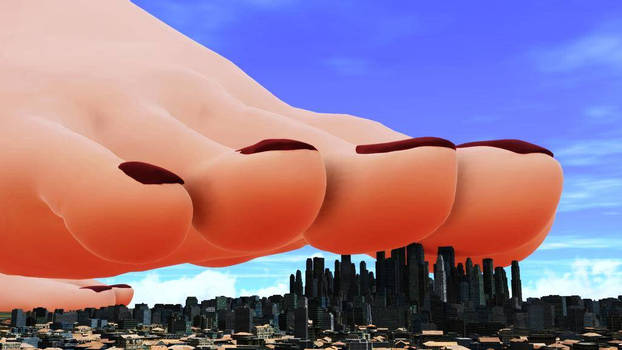
\includegraphics[scale=0.7,natwidth=10,natheight=10]{Pictures/infinity.jpg}}
%\newcommand{\normal}{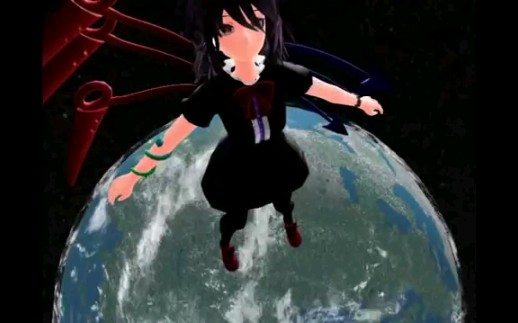
\includegraphics[scale=0.7,natwidth=10,natheight=10]{Pictures/normal.jpg}}
%\newcommand{\boss}{
\includegraphics[scale=0.13,natwidth=10,natheight=10]{Pictures/boss.png}}
%\newcommand{\collision}{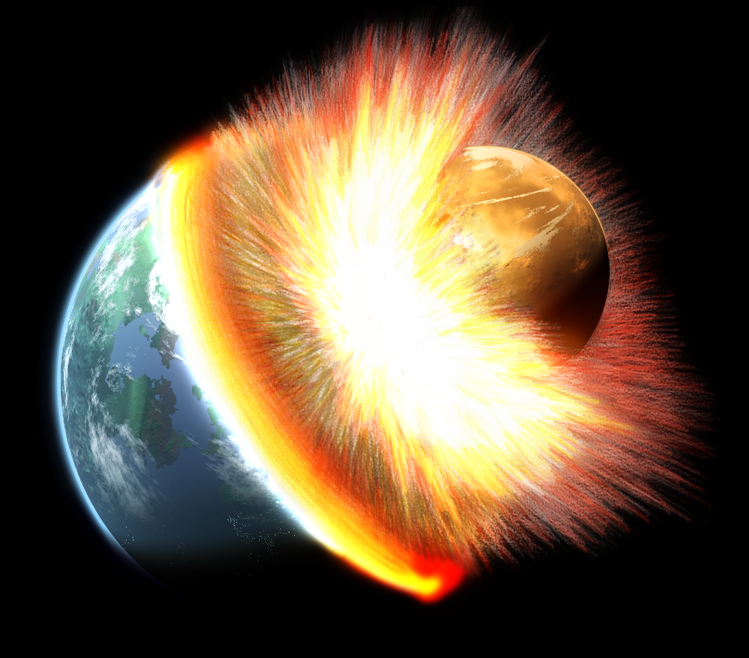
\includegraphics[scale=0.5,natwidth=10,natheight=10]{Pictures/collision.png}}
%\newcommand{\homework}{
\includegraphics[scale=0.13,natwidth=10,natheight=10]{Pictures/homework.png}}
%\newcommand{\sinister}{
\includegraphics[scale=0.13,natwidth=10,natheight=10]{Pictures/sinister.png}}
%\newcommand{\sleep}{
\includegraphics[scale=0.13,natwidth=10,natheight=10]{Pictures/sleep.png}}
%\newcommand{\answer}{
\includegraphics[scale=0.13,natwidth=10,natheight=10]{Pictures/answer.png}}
%\newcommand{\hi}{
\includegraphics[scale=0.13,natwidth=10,natheight=10]{Pictures/hi.png}}
%\newcommand{\spy}{
\includegraphics[scale=0.04,natwidth=10,natheight=10]{Pictures/spy.png}}
%\newcommand{\police}{
\includegraphics[scale=0.2,natwidth=10,natheight=10]{Pictures/police.png}}
%\newcommand{\case}{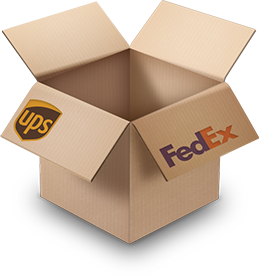
\includegraphics[scale=0.1,natwidth=10,natheight=10]{Pictures/box.png}}
%\newcommand{\remote}{
\includegraphics[scale=0.05,natwidth=10,natheight=10]{Pictures/remote.png}}
%\newcommand{\wifi}{
\includegraphics[scale=0.05,natwidth=10,natheight=10]{Pictures/wifi.png}}
%\newcommand{\man}{
\includegraphics[scale=0.1,natwidth=10,natheight=10]{Pictures/man.png}}
%\newcommand{\bow}{
\includegraphics[scale=0.08,natwidth=10,natheight=10]{Pictures/bow.jpg}}
%\newcommand{\house}{
\includegraphics[scale=0.13,natwidth=10,natheight=10]{Pictures/house.png}}
%\newcommand{\convey}{\includegraphics[scale=0.13,natwidth=10,natheight=10]{Pictures/convey.jpg}}

%%%%%%%%%%%%%%%% The above are for pictures %%%%%%%%%%%%%%%%%%%%%%
%%%%%%%%%%%%%%%%%%%%%%%%%%%%%%%%%%%%%%%%%%%%%%%%%%%%%%%%%%%%%%%%%

\long\def\[#1]#2{ \begin{#1}#2\end{#1}}
\makeatletter
\def\m{\@tut\@gobble\@tutt}
\def\@tut#1\@tutt#2{
\@ifnextchar,{\@tut #1 & #2\\\expandafter\expandafter\expandafter\@gobble\expandafter\@gobble\@gobble\@tutt}{
\@ifnextchar.{\begin{pmatrix}#1 &#2\end{pmatrix}\@gobble}{\@tut #1 & #2\@tutt}
}
}
\def\bm{\@tuut\@gobble\@tuutt}
\def\@tuut#1\@tuutt#2{
\@ifnextchar,{\@tuut #1 & #2\cr\expandafter\expandafter\expandafter\@gobble\expandafter\@gobble\@gobble\@tuutt}{
\@ifnextchar.{\bordermatrix{#1 &#2\cr}\@gobble}{\@tuut #1 & #2\@tuutt}
}
}
\makeatother

%%%%% The following are command folders
%\input{Command/script}

%\input{Command/infinity}
\newcommand{\n}{{\color{blue}0}}
\newcommand{\w}{{\color{red}\infty}}
\newcommand{\ac}[1]{\qquad (\; \n^{#1} = 0\; )}
\newcommand{\cn}[1]{\cdot\n^{#1}}

%\input{Command/Drawer}


\newcommand\ko[4]{\begin{scope}[scale=0.5,xshift=#1 cm,yshift=#2 cm]
#3#4
\end{scope}}

\newcommand\dback{
% following 后面
\draw[white,fill={rgb:red,5;green,2;yellow,5}] (10,2)--(6,2)--(6,3)--(12,3);
%following 底面
\draw[white,fill={rgb:red,8;green,1;yellow,8}] (2,0)--(6,0)--(10,2)--(6,2)--(2,0);
\draw[black] (10,2)--(6,2)--(2,0);
% following 内左侧面
\draw[white,fill={rgb:red,5;green,3;yellow,1}] (0,0)--(6,3)--(6,2)--(2,0);
}

\newcommand\dfront{

%following 右侧面
\draw[white,fill={rgb:red,5;green,3;yellow,1}] (6,0)--(12,3)--(12,2)--(6,-1)--(6,0);
% Following the 前面
\draw[white, fill={rgb:red,4;green,2;yellow,1}] (0,0)--(6,0)--(6,-1)--(0,-1)--(0,0);
\draw[white,fill=white] (2,-0.3)--(4,-0.3)--(4,-0.4)--(2,-0.4)--(2,-0.3);
}

\newcommand\nb[1]{\node[shape=circle,fill=white,inner sep=0.5pt] at (0,0) {\textcolor{black}{#1}};}
\newcommand\nw[1]{\node[shape=circle,fill=black,inner sep=0.5pt] at (0,0) {\textcolor{white}{#1}};}
\newcommand\nnw[3]{\node[shape=circle,fill=black,inner sep=0.5pt] at (#2,#3) {\textcolor{white}{#1}};}

\newcommand\bo[1]{
\draw[fill=#1]  (0,0)--(2,0)--(4,1)--(2,1)--(0,0)--(0,-0.3)--(2,-0.3)--(4,0.7)--(4,1);
}

\newcommand\boo[2]{
\draw[fill=#1]  (0,0)--(2,0)--(4,1)--(2,1)--(0,0)--(0,-0.3)--(2,-0.3)--(4,0.7)--(4,1);
\node[shape=circle,fill=white,inner sep=0.5pt] at (2,1) {\textcolor{black}{#2}};
}

\newcommand\booo[3]{
\draw[fill=#1]  (0,0)--(2,0)--(4,1)--(2,1)--(0,0)--(0,-0.3)--(2,-0.3)--(4,0.7)--(4,1);
\node[shape=circle,fill=white,inner sep=0.5pt] at (2,1) {\textcolor{black}{#2}};
\node[shape=circle,fill=white,inner sep=0.5pt] at (2.5,1) {\textcolor{black}{#3}};
}

\newcommand\boooo[4]{
\draw[fill=#1]  (0,0)--(2,0)--(4,1)--(2,1)--(0,0)--(0,-0.3)--(2,-0.3)--(4,0.7)--(4,1);
\node[shape=circle,fill=white,inner sep=0.5pt] at (2,1) {\textcolor{black}{#2}};
\node[shape=circle,fill=white,inner sep=0.5pt] at (2.5,1) {\textcolor{black}{#3}};
\node[shape=circle,fill=white,inner sep=0.5pt] at (3,1) {\textcolor{black}{#4}};
}


\newcommand\booooo[5]{
\draw[fill=#1]  (0,0)--(2,0)--(4,1)--(2,1)--(0,0)--(0,-0.3)--(2,-0.3)--(4,0.7)--(4,1);
\node[shape=circle,fill=white,inner sep=0.5pt] at (2,1) {\textcolor{black}{#2}};
\node[shape=circle,fill=white,inner sep=0.5pt] at (2.5,1) {\textcolor{black}{#3}};
\node[shape=circle,fill=white,inner sep=0.5pt] at (3,1) {\textcolor{black}{#4}};
\node[shape=circle,fill=white,inner sep=0.5pt] at (3.5,1) {\textcolor{black}{#5}};
}





\newcommand\bbo[2]{
\draw[fill=#1]  (0,0)--(2,0)--(4,1)--(2,1)--(0,0)--(0,-0.3)--(2,-0.3)--(4,0.7)--(4,1);
\node[shape=circle,fill=black,inner sep=0.5pt] at (1,0.5) {\textcolor{white}{#2}};
}

\newcommand\bboo[3]{
\draw[fill=#1]  (0,0)--(2,0)--(4,1)--(2,1)--(0,0)--(0,-0.3)--(2,-0.3)--(4,0.7)--(4,1);
\node[shape=circle,fill=white,inner sep=0.5pt] at (2,1) {\textcolor{black}{#2}};
\node[shape=circle,fill=black,inner sep=0.5pt] at (1,0.5) {\textcolor{white}{#3}};
}

\newcommand\bbooo[4]{
\draw[fill=#1]  (0,0)--(2,0)--(4,1)--(2,1)--(0,0)--(0,-0.3)--(2,-0.3)--(4,0.7)--(4,1);
\node[shape=circle,fill=white,inner sep=0.5pt] at (2,1) {\textcolor{black}{#2}};
\node[shape=circle,fill=white,inner sep=0.5pt] at (2.5,1) {\textcolor{black}{#3}};
\node[shape=circle,fill=black,inner sep=0.5pt] at (1,0.5) {\textcolor{white}{#4}};
}

\newcommand\bboooo[5]{
\draw[fill=#1]  (0,0)--(2,0)--(4,1)--(2,1)--(0,0)--(0,-0.3)--(2,-0.3)--(4,0.7)--(4,1);
\node[shape=circle,fill=white,inner sep=0.5pt] at (2,1) {\textcolor{black}{#2}};
\node[shape=circle,fill=white,inner sep=0.5pt] at (2.5,1) {\textcolor{black}{#3}};
\node[shape=circle,fill=white,inner sep=0.5pt] at (3,1) {\textcolor{black}{#4}};
\node[shape=circle,fill=black,inner sep=0.5pt] at (1,0.5) {\textcolor{white}{#5}};
}


\newcommand\bbooooo[6]{
\draw[fill=#1]  (0,0)--(2,0)--(4,1)--(2,1)--(0,0)--(0,-0.3)--(2,-0.3)--(4,0.7)--(4,1);
\node[shape=circle,fill=white,inner sep=0.5pt] at (2,1) {\textcolor{black}{#2}};
\node[shape=circle,fill=white,inner sep=0.5pt] at (2.5,1) {\textcolor{black}{#3}};
\node[shape=circle,fill=white,inner sep=0.5pt] at (3,1) {\textcolor{black}{#4}};
\node[shape=circle,fill=white,inner sep=0.5pt] at (3.5,1) {\textcolor{black}{#5}};
\node[shape=circle,fill=black,inner sep=0.5pt] at (1,0.5) {\textcolor{white}{#6}};
}

\newcommand\bbbo[3]{
\draw[fill=#1]  (0,0)--(2,0)--(4,1)--(2,1)--(0,0)--(0,-0.3)--(2,-0.3)--(4,0.7)--(4,1);
\node[shape=circle,fill=black,inner sep=0.5pt] at (1,0.5) {\textcolor{white}{#2}};
\node[shape=circle,fill=black,inner sep=0.5pt] at (1.5,0.5) {\textcolor{white}{#3}};
}

\newcommand\bbboo[4]{
\draw[fill=#1]  (0,0)--(2,0)--(4,1)--(2,1)--(0,0)--(0,-0.3)--(2,-0.3)--(4,0.7)--(4,1);
\node[shape=circle,fill=white,inner sep=0.5pt] at (2,1) {\textcolor{black}{#2}};
\node[shape=circle,fill=black,inner sep=0.5pt] at (1,0.5) {\textcolor{white}{#3}};
\node[shape=circle,fill=black,inner sep=0.5pt] at (1.5,0.5) {\textcolor{white}{#4}};
}

\newcommand\bbbooo[5]{
\draw[fill=#1]  (0,0)--(2,0)--(4,1)--(2,1)--(0,0)--(0,-0.3)--(2,-0.3)--(4,0.7)--(4,1);
\node[shape=circle,fill=white,inner sep=0.5pt] at (2,1) {\textcolor{black}{#2}};
\node[shape=circle,fill=white,inner sep=0.5pt] at (2.5,1) {\textcolor{black}{#3}};
\node[shape=circle,fill=black,inner sep=0.5pt] at (1,0.5) {\textcolor{white}{#4}};
\node[shape=circle,fill=black,inner sep=0.5pt] at (1.5,0.5) {\textcolor{white}{#5}};
}

\newcommand\bbboooo[6]{
\draw[fill=#1]  (0,0)--(2,0)--(4,1)--(2,1)--(0,0)--(0,-0.3)--(2,-0.3)--(4,0.7)--(4,1);
\node[shape=circle,fill=white,inner sep=0.5pt] at (2,1) {\textcolor{black}{#2}};
\node[shape=circle,fill=white,inner sep=0.5pt] at (2.5,1) {\textcolor{black}{#3}};
\node[shape=circle,fill=white,inner sep=0.5pt] at (3,1) {\textcolor{black}{#4}};
\node[shape=circle,fill=black,inner sep=0.5pt] at (1,0.5) {\textcolor{white}{#5}};
\node[shape=circle,fill=black,inner sep=0.5pt] at (1.5,0.5) {\textcolor{white}{#6}};
}


\newcommand\bbbooooo[7]{
\draw[fill=#1]  (0,0)--(2,0)--(4,1)--(2,1)--(0,0)--(0,-0.3)--(2,-0.3)--(4,0.7)--(4,1);
\node[shape=circle,fill=white,inner sep=0.5pt] at (2,1) {\textcolor{black}{#2}};
\node[shape=circle,fill=white,inner sep=0.5pt] at (2.5,1) {\textcolor{black}{#3}};
\node[shape=circle,fill=white,inner sep=0.5pt] at (3,1) {\textcolor{black}{#4}};
\node[shape=circle,fill=white,inner sep=0.5pt] at (3.5,1) {\textcolor{black}{#5}};
\node[shape=circle,fill=black,inner sep=0.5pt] at (1,0.5) {\textcolor{white}{#6}};
\node[shape=circle,fill=black,inner sep=0.5pt] at (1.5,0.5) {\textcolor{white}{#7}};
}

%\input{Command/ProofControl}
\newif\ift\ttrue
\newif\ifs\strue
\newif\ifi\itrue
\newcommand{\ii}{\ifi}
\newcommand{\iii}{\fi}
\newcommand{\tp}{\ift \textbf{Proof:}}
\newcommand{\app}{\ift \textbf{Standard Proof:}}
\newcommand{\pppp}{\a\aa\textbf{Proof continue }}
\newcommand{\pt}{\fi$\blacksquare$}
\newcommand{\ppa}{\fi$\blacksquare$}
%\input{Command/Tags}
\newcommand*\circled[1]{\tikz[baseline=(char.base)]{
            \node[shape=circle,fill,inner sep=2pt] (char) {\textcolor{white}{#1}};}}
\newcommand*\bl[1]{\tikz[baseline=(char.base)]{
            \node[shape=circle,fill,inner sep=2pt] (char) {\textcolor{white}{#1}};}}
\newcommand*\wh[1]{\tikz[baseline=(char.base)]{
            \node[shape=circle,draw,inner sep=2pt] (char) {#1};}}
%\input{Command/Classify}
\newcommand{\classify}[1]{\fbox{\footnotesize{}$#1$}}
\newcommand{\LI}{{\color{red}\classify{L_I}}}
\newcommand{\II}{{\color{red}\classify{I}}}
\newcommand{\CI}{{\color{red}\classify{C_I}}}
\newcommand{\DI}{{\color{red}\classify{D_I}}}
\newcommand{\NI}{{\color{red}\classify{N_I}}}
\newcommand{\RI}{{\color{red}\classify{R_I}}}
\newcommand{\LS}{{\color{blue}\classify{L_S}}}
\renewcommand{\SS}{{\color{blue}\classify{S}}}
\newcommand{\CS}{{\color{blue}\classify{C_S}}}
\newcommand{\DS}{{\color{blue}\classify{D_S}}}
\newcommand{\NS}{{\color{blue}\classify{N_S}}}
\newcommand{\RS}{{\color{blue}\classify{R_S}}}
%\input{Command/Conveyor}
\pgfmathsetmacro\stack{0}
\def\levelup{\elevate1}%Defalt Value
\def\elevate#1{\pgfmathsetmacro\stack{\stack+1.2*#1}}
\def\su#1{\def\elevate##1{\pgfmathsetmacro\stack{\stack+#1*##1}}}


\pgfmathsetmacro\LeftShift{0}
\pgfmathsetmacro\LeftBox{0}
\def\sb#1{\pgfmathsetmacro\LeftBox{\LeftShift+1.5*#1}}
\def\sf#1{\pgfmathsetmacro\LeftShift{\LeftShift+1.5*#1}}%Defalt Value

\def\B#1{
\abox0\stack{#1}
\levelup
}
\def\BB#1#2{
\abox0\stack{#1}\abox1\stack{#2}
\levelup
}
\def\BBB#1#2#3{
\abox0\stack{#1}\abox1\stack{#2}\abox2\stack{#3}
\levelup
}
\def\BBBB#1#2#3#4{
\abox0\stack{#1}\abox1\stack{#2}\abox2\stack{#3}\abox3\stack{#4}
\levelup
}
\def\BBBBB#1#2#3#4#5{
\abox0\stack{#1}\abox1\stack{#2}\abox2\stack{#3}\abox3\stack{#4}\abox4\stack{#5}
\levelup
}

\def\setgearlevel{\pgfmathsetmacro\gearlevel{\stack-0.1}}

\def\g#1{\setgearlevel
\agear0\gearlevel{#1}\track0\gearlevel0}



\def\gg#1#2{\setgearlevel
\agear0\gearlevel{#1}
\agear1\gearlevel{#2}
\track0\gearlevel1}

\def\ggg#1#2#3{\setgearlevel
\agear0\gearlevel{#1}
\agear1\gearlevel{#2}
\agear2\gearlevel{#3}
\track0\gearlevel2}

\def\gggg#1#2#3#4{\setgearlevel
\agear0\gearlevel{#1}
\agear1\gearlevel{#2}
\agear2\gearlevel{#3}
\agear3\gearlevel{#4}
\track0\gearlevel3}

\def\ggggg#1#2#3#4#5{\setgearlevel
\agear0\gearlevel{#1}
\agear1\gearlevel{#2}
\agear2\gearlevel{#3}
\agear3\gearlevel{#4}
\agear4\gearlevel{#5}
\track0\gearlevel4}

\def\gggggg#1#2#3#4#5#6{\setgearlevel
\agear0\gearlevel{#1}
\agear1\gearlevel{#2}
\agear2\gearlevel{#3}
\agear3\gearlevel{#4}
\agear4\gearlevel{#5}
\agear5\gearlevel{#6}
\track0\gearlevel5}

\def\ggggggg#1#2#3#4#5#6#7{\setgearlevel
\agear0\gearlevel{#1}
\agear1\gearlevel{#2}
\agear2\gearlevel{#3}
\agear3\gearlevel{#4}
\agear4\gearlevel{#5}
\agear5\gearlevel{#6}
\agear6\gearlevel{#7}
\track0\gearlevel6}

\def\gggggggg#1#2#3#4#5#6#7#8{\setgearlevel
\agear0\gearlevel{#1}
\agear1\gearlevel{#2}
\agear2\gearlevel{#3}
\agear3\gearlevel{#4}
\agear4\gearlevel{#5}
\agear5\gearlevel{#6}
\agear6\gearlevel{#7}
\agear7\gearlevel{#8}
\track0\gearlevel7}

\def\ggggggggg#1#2#3#4#5#6#7#8#9{\setgearlevel
\agear0\gearlevel{#1}
\agear1\gearlevel{#2}
\agear2\gearlevel{#3}
\agear3\gearlevel{#4}
\agear4\gearlevel{#5}
\agear5\gearlevel{#6}
\agear6\gearlevel{#7}
\agear7\gearlevel{#8}
\agear8\gearlevel{#9}
\track0\gearlevel8}





\def\abox#1#2#3{%#1=Left position, #2=Top position, #3= Node
    \pgfmathsetmacro\w{#1*1.5}
    \pgfmathsetmacro\p{#2}
    \fill[xshift=-0.5 cm,xshift=\LeftBox cm,yshift=.5cm,rounded corners,red] (\w,\p) node[ultra thick,white,minimum size=12pt] at (\w+0.5,\p+0.5) {\Large #3} rectangle (\w+1,\p+1) ;
}
\def\bbox#1#2#3{%#1=Left position, #2=Top position, #3= Node
    \pgfmathsetmacro\w{#1*1.5}
    \pgfmathsetmacro\p{#2}
    \fill[xshift=-0.5 cm,xshift=\LeftBox cm,yshift=.5cm,rounded corners,fill=pur] (\w,\p) node[ultra thick,white,minimum size=12pt] at (\w+0.5,\p+0.5) {\Large #3} rectangle (\w+1,\p+1) ;
}
\def\cbox#1#2#3{%#1=Left position, #2=Top position, #3= Node
    \pgfmathsetmacro\w{#1*1.5}
    \pgfmathsetmacro\p{#2}
    \fill[xshift=-0.5 cm,xshift=\LeftBox cm,yshift=.5cm,rounded corners,blue] (\w,\p) node[ultra thick,white,minimum size=12pt] at (\w+0.5,\p+0.5) {\Large #3} rectangle (\w+1,\p+1) ;
}
\def\aB#1#2{
\elevate{-1}
\abox#1\stack{#2}
\levelup
}

\def\bB#1#2{
\elevate{-1}
\bbox#1\stack{#2}
\levelup
}
\def\cB#1#2{
\elevate{-1}
\cbox#1\stack{#2}
\levelup
}




\def\track#1#2#3{%This is a track over the gear
\pgfmathsetmacro\w{#1*1.5}
\pgfmathsetmacro\p{#2}
\pgfmathsetmacro\sha{#3*1.5}
\draw[ultra thick,xshift=\w+\LeftShift cm, yshift=\p cm] (0,.5) -- (\sha,.5) arc(90:-90:.5) -- (0,-.5) arc(-90:-270:.5);
\draw[->, thick,blue,xshift=\w+\LeftShift cm, yshift=\p cm] (1,-.7)--(0,-.7) arc(270:90:.7);
\sb0
}


\def\agear#1#2#3{%#1=Left position, #2=Top position, #3= Node
 \pgfmathsetmacro\n{10}%齿轮旋转的角度
    \def\sawtooth{8}
    \pgfmathsetmacro\w{#1*1.5+\LeftShift}
    \pgfmathsetmacro\p{#2}
    \foreach \m in {0,1,...,\sawtooth}
        {\pgfmathsetmacro\x{\m*360/\sawtooth}
         \fill (\w,\p) -- ([xshift=\w cm,yshift=\p cm]\x+\n:.5) arc(\x+\n:\x+\n+20:.5) -- cycle;
    }%这是齿部分
        \fill (\w,\p) circle(.4) node[ultra thick,white,minimum size=12pt] at (\w,\p) { #3};
}

\def\anode#1#2{
    \node[ultra thick,white,minimum size=12pt] at (#1,0) {\Large #2};
}

\def\boxes#1{
    \pgfmathsetmacro\sha{#1-1}
    \foreach \k in {0,...,\sha}{\abox\k0{2}}
}
%\input{Command/Tableau}
\newcommand{\nl}[2]{\dim\left(\ker(#1^{#2})\right)}
\newcommand{\td}{
{Tableau Direction} 

\[zzz]{\B{$\ww$}\B{$\vv$}}
:$\ww=T\vv$
}
\newcommand{\TD}{
{\bf \text{Tableau Direction }}
\ytableaushort{\ww\vv}:$\ww=T\vv$
}
\newcommand{\TDD}[1]{
{\bf \text{Tableau Direction }}

\ytableaushort{\ww\vv}:$\ww=#1\vv$
}

\newcommand{\yt}{\ytableaushort}
\newcommand{\yd}{\ydiagram}
\newcommand{\ys}{\ytableausetup{mathmode, boxsize=1em}}
\newcommand{\ym}{\ytableausetup{mathmode, boxsize=1.5em}}
\newcommand{\yl}{\ytableausetup{mathmode, boxsize=2.5em}}
\newcommand{\yll}{\ytableausetup{mathmode, boxsize=4.5em}}
%\input{Command/convenient}
\newcommand{\mogui}{\vfill{\small\color{gray}\exe Prove this without using \idu\lt.}}
\newcommand\nothing[1]{#1}
%\input{Command/AdjointOperators}
\newcommand{\ttvw}{$\map{T^*}WV$ }
\newcommand{\ssvw}{$\map{S^*}WV$ }
\newcommand{\tvw}{$\map TVW$ }
\newcommand{\svw}{$\map SVW$ }
\newcommand{\swu}{$\map SWU$}
\newcommand{\tvv}{$\map TVV$ }
\newcommand{\vV}{$\vv\in V$ }
\newcommand{\wW}{$\ww\in W$ }
\newcommand{\uU}{$\uu\in U$ }
\newcommand{\adj}{^*}
\newcommand{\pr}[1]{\mathrm{Proj}_{#1}}
\newcommand{\oc}{^\perp}

%\input{Command/Terminology}
\newcommand{\eve}{eigenvector }
\newcommand{\nmo}{normal operator }
\newcommand{\ebas}{eigenbasis }
\newcommand{\oebas}{orthonormal eigenbasis }
\newcommand{\sa}{Self adjoint }
\newcommand{\ut}{unitary }
\newcommand{\op}{Othogonal projection }
\newcommand{\pro}{\textbf{Proof}}
\newcommand{\zs}{\{\0\}}

\newcommand{\idu}{ induced }
\newcommand{\lcb}{ linear combination }

\newcommand{\ldr}{ linear dependence relation }
%\input{Command/Interval}
\newcommand{\qj}[3]{#2<#1<#3}
%\input{Command/index}
\newcommand\nata[3]{L_{\nota{#1}{#2}{#3}}}
%\input{Command/forsome}
\newcommand{\forsome}[2]{
	\qquad \text{for some }#1_1,\cdots,#1_#2\in F
	}
%\vfill

% The following is for Calculus teaching
%The following is for problem making
\newcommand{\baspoly}{ $\{1,x,x^2\}$ is a basis for $V$ }
\newcommand{\polypro}[1]{Let $V=\lPP xabc$, $\map TVV$ is a linear operator defined by $T[f](x)=#1$ }
\newcommand{\polyprot}[1]{Let $V=\lPP xabc$, $W=\lPP tabc$, $\map TVW$ is a linear map defined by $T:f(x)\mapsto #1$ }

\newcommand{\nota}[3]{\left[#1\right]_{#2}^{#3}}
\newcommand{\notaw}[3]{\left[#1\right]^{#2}_{#3}}





%The following is for polynomial notations
\newcommand{\Field}{F}
\newcommand{\lPP}[4]{P_{2,#1}=\{#2#1^2+#3#1+#4,\text{ where }#2,#3,#4\in \Field\}}
\newcommand{\lP}[3]{P_{1,#1}=\{#2#1+#3,\text{ where }#2,#3\in \Field\}}
\newcommand{\lPPP}[5]{P_{3,#1}=\{#2#1^3+#3#1^2+#4#1+#5,\text{ where }#2,#3,#4,#5\in \Field\}}
\newcommand{\f}{\mathrm{F}}
% The following is for existence uniqueness argument
\newcommand{\ch}{\mathrm{char}}
\newcommand{\ce}{{\mathcal E}}
\newcommand{\cw}{{\mathcal F}}
\newcommand{\cv}{{\mathcal G}}
\newcommand{\cd}{{\mathcal H}}
\newcommand{\be}[1]{\mathcal{E}=\basis \ee#1}
\newcommand{\bw}[1]{\mathcal{F}=\basis \ww#1}
\newcommand{\bv}[1]{\mathcal{G}=\basis \vv#1}
\newcommand{\bd}[1]{\mathcal{H}=\basis{\vec d}#1}
\newcommand{\uu}{\vec{u}}
\newcommand{\obe}[1]{\obasis \ee#1}
\newcommand{\obw}[1]{\obasis \ww#1}
\newcommand{\obv}[1]{\obasis \vv#1}
\newcommand{\obd}[1]{\obasis{\vec d}#1}
\definecolor{pur}{RGB}{255,0,255}

\newcommand{\spa}{\textbf{ span }}
\newcommand{\spab}{\textbf{ spanned by }}


\newcommand{\bn}{\textbf{\color{blue} Numerical Property }}
\newcommand{\sws}{\textbf{\color{blue} span the whole space }}
%\newcommand{\sws}{\textbf{\color{blue} 张满全空间 }}
\newcommand{\swss}{\textbf{\color{blue} span the whole subspace }}
\newcommand{\te}{\textbf{\color{blue} there exists }}
\newcommand{\ifu}{\textbf{\color{blue} but may not unique }}
\newcommand{\stws}{\textbf{\color{blue} sum to the whole space }}



\newcommand{\SI}{{\color{blue}\classify{{\color{blue}S}\mapsto{\color{red}I}}}}
\newcommand{\IS}{{\color{red}\classify{{\color{red}I}\mapsto{\color{blue}S}}}}

\newcommand{\exce}{\textbf{\color{blue} existence }}
\newcommand{\scy}{\textbf{\color{blue} sufficiency }}
%\newcommand{\exce}{\textbf{\color{blue} 存在性 }}
\newcommand{\enu}{\textbf{\color{blue} constructive language }}
%\newcommand{\enu}{\textbf{\color{blue} 枚举性语言}}
\newcommand{\enuv}{\textbf{\color{blue} constructive} }
%\newcommand{\enuv}{\textbf{\color{blue} 枚举性的}}

\newcommand{\leasto}{\textbf{\color{blue} at least one }}
%\newcommand{\leasto}{\textbf{\color{blue} 至少有一个 }}
\newcommand{\exi}{\textbf{\color{blue} exists }}
%\newcommand{\exi}{\textbf{\color{blue} 存在 }}
\newcommand{\more}{\textbf{\color{blue} no less than }}
\newcommand{\nored}{\textbf{\color{blue} independent equations }}
\newcommand{\exx}{\textbf{\color{blue} 有 }}
\newcommand{\excp}{\textbf{\color{blue} existence problem }}
\newcommand{\rc}{\textbf{\color{blue} right cancellation }}
%\newcommand{\rc}{\textbf{\color{blue} 可右消去}}
\newcommand{\rf}{\textbf{\color{blue} right factor }}
%\newcommand{\rf}{\textbf{\color{blue} 右因子 }}
\newcommand{\riv}{\textbf{\color{blue} right inverse }}


\newcommand{\sub}{\textbf{\color{blue} sub}}


\newcommand{\sur}{\textbf{\color{blue} surjective }}
%\newcommand{\sur}{\textbf{\color{blue} 满射 }}
\newcommand{\pa}{\textbf{\color{blue} parameters }}
%\newcommand{\pa}{\textbf{\color{blue}参数}}
\newcommand{\pation}{\textbf{\color{black} parametrization }}

\newcommand{\img}{\textbf{\color{black} image }}

\newcommand{\rn}{\textbf{\color{red} Numerical Property }}
\newcommand{\des}{\textbf{\color{red} descriptive language }}
%\newcommand{\des}{\textbf{\color{red} 概括性语言}}
\newcommand{\desv}{\textbf{\color{red} descriptive }}
%\newcommand{\desv}{\textbf{\color{red} 概括性的}}

\newcommand{\unce}{\textbf{\color{red} uniqueness }}
%\newcommand{\unce}{\textbf{\color{red} 唯一性 }}
\newcommand{\ecy}{\textbf{\color{red} ecnomical }}
\newcommand{\mosto}{\textbf{\color{red} at most one }}
%\newcommand{\mosto}{\textbf{\color{red} 至多有一个 }}
\newcommand{\less}{\textbf{\color{red} no more than }}
\newcommand{\ife}{\textbf{\color{red} if there exists }}
\newcommand{\un}{\textbf{\color{red} unique }}
\newcommand{\uny}{\textbf{\color{red} uniquely }}
\newcommand{\nofree}{\textbf{\color{red} no free variables }}
%\newcommand{\un}{\textbf{\color{red} 唯一 }}
\newcommand{\unp}{\textbf{\color{red} uniqueness problem }}
\newcommand{\lc}{\textbf{\color{red} left cancellation }}
%\newcommand{\lc}{\textbf{\color{red} 可左消去 }}
\newcommand{\lf}{\textbf{\color{red} left factor }}
%\newcommand{\lf}{\textbf{\color{red} 左因子 }}
\newcommand{\liv}{\textbf{\color{red} left inverse }}

\newcommand{\quo}{\textbf{\color{red} quotient}}

\newcommand{\inj}{\textbf{\color{red} injective }}
%\newcommand{\inj}{\textbf{\color{red} 单射 }}
\newcommand{\cla}{\textbf{\color{red}class }}
\newcommand{\cl}{\textbf{\color{red}property }}
%\newcommand{\cla}{\textbf{\color{red}类别}}
\newcommand{\clation}{\textbf{\color{black}classification}}
\newcommand{\li}{\textbf{\color{red} linealy independent }}
%\newcommand{\li}{\textbf{\color{red} 线性独立 }}
\newcommand{\ids}{\textbf{\color{red} is a direct sum }}


\newcommand{\pimg}{\textbf{\color{black} preimage }}
\newcommand{\kn}{\textbf{\color{red} kernel }}

\newcommand{\iso}{\textbf{\color{pur} isomorphism }}
%\newcommand{\iso}{\textbf{\color{pur} 双射 }}
\newcommand{\teun}{\textbf{\color{pur} there exists an unique }}
%\newcommand{\teun}{\textbf{\color{pur} 存在唯一 }}
\newcommand{\eeun}{\textbf{\color{pur} 唯一指定 }}
\newcommand{\exacto}{\textbf{\color{pur} exactly one }}
%\newcommand{\exacto}{\textbf{\color{pur} 恰好有一个 }}
\newcommand{\bas}{\textbf{\color{pur} basis }}
%\newcommand{\bas}{\textbf{\color{pur} 基 }}
\newcommand{\dstws}{\textbf{\color{pur} direct sum to the whole space }}
\newcommand{\dst}{\textbf{\color{pur} direct sum decomposition }}
\newcommand{\inve}{\textbf{\color{pur} invertible }}
\newcommand{\same}{\textbf{\color{pur} is the same as }}
%\newcommand{\inve}{\textbf{\color{pur} 可逆 }}
\newcommand{\pn}{\textbf{\color{pur} Numerical Property }}
\newcommand{\np}{\textbf{\color{pur} No Problem }}

\newcommand{\lt}{linear transformation }
\newcommand{\lo}{linear operator }
\newcommand{\rs}{restriction }
\newcommand{\sus}{subspace }
\newcommand{\insus}{invariant subspace }
\newcommand{\ges}{generalized eigenspace }
\newcommand{\ev}{eigenvalue }
\newcommand{\cp}{characteristic polynomial }

% The following is for pictures

\newcommand{\bb}{\x}
\newcommand{\apple}{\includegraphics[scale=0.08,natwidth=10,natheight=10]{Pictures/apple.png}}
\newcommand{\bigapple}{\includegraphics[scale=0.13,natwidth=10,natheight=10]{Pictures/apple.png}}
\newcommand{\peach}{\includegraphics[scale=0.08,natwidth=10,natheight=10]{Pictures/peach.png}}
\newcommand{\bigpeach}{\includegraphics[scale=0.13,natwidth=10,natheight=10]{Pictures/peach.png}}
\newcommand{\bean}{\includegraphics[scale=0.07,natwidth=10,natheight=10]{Pictures/bean.png}}
\newcommand{\sbean}{\includegraphics[scale=0.04,natwidth=10,natheight=10]{Pictures/bean.png}}
\newcommand{\soup}{\includegraphics[scale=0.10,natwidth=10,natheight=10]{Pictures/soup.png}}
\newcommand{\ssoup}{\includegraphics[scale=0.07,natwidth=10,natheight=10]{Pictures/soup.png}}
\newcommand{\bigsoup}{\includegraphics[scale=0.30,natwidth=10,natheight=10]{Pictures/soup.png}}
\newcommand{\lemon}{\includegraphics[scale=0.08,natwidth=10,natheight=10]{Pictures/lemon.png}}
\newcommand{\slemon}{\includegraphics[scale=0.05,natwidth=10,natheight=10]{Pictures/lemon.png}}
\newcommand{\biglemon}{\includegraphics[scale=0.13,natwidth=10,natheight=10]{Pictures/lemon.png}}
\newcommand{\leaf}{\includegraphics[scale=0.08,natwidth=10,natheight=10]{Pictures/leaf.png}}
\newcommand{\sleaf}{\includegraphics[scale=0.05,natwidth=10,natheight=10]{Pictures/leaf.png}}
\newcommand{\milk}{\includegraphics[scale=0.07,natwidth=10,natheight=10]{Pictures/milk.png}}
\newcommand{\smilk}{\includegraphics[scale=0.04,natwidth=10,natheight=10]{Pictures/milk.png}}
\newcommand{\coffee}{\includegraphics[scale=0.10,natwidth=10,natheight=10]{Pictures/coffee.png}}
\newcommand{\scoffee}{\includegraphics[scale=0.07,natwidth=10,natheight=10]{Pictures/coffee.png}}
\newcommand{\carrot}{\includegraphics[scale=0.11,natwidth=10,natheight=10]{Pictures/carrot.png}}
\newcommand{\bigcarrot}{\includegraphics[scale=0.15,natwidth=10,natheight=10]{Pictures/carrot.png}}
\newcommand{\cola}{\includegraphics[scale=0.08,natwidth=10,natheight=10]{Pictures/cola.png}}
\newcommand{\scola}{\includegraphics[scale=0.05,natwidth=10,natheight=10]{Pictures/cola.png}}
\newcommand{\tea}{\includegraphics[scale=0.08,natwidth=10,natheight=10]{Pictures/tea.png}}
\newcommand{\stea}{\includegraphics[scale=0.05,natwidth=10,natheight=10]{Pictures/tea.png}}
\newcommand{\teaa}{\includegraphics[scale=0.03,natwidth=10,natheight=10]{Pictures/teaaa.jpg}}
\newcommand{\cow}{\includegraphics[scale=0.08,natwidth=10,natheight=10]{Pictures/cow.png}}
\newcommand{\orange}{\includegraphics[scale=0.09,natwidth=10,natheight=10]{Pictures/orange.png}}
\newcommand{\bento}{\includegraphics[scale=0.09,natwidth=10,natheight=10]{Pictures/bento.png}}
\newcommand{\sbento}{\includegraphics[scale=0.04,natwidth=10,natheight=10]{Pictures/bento.png}}
\newcommand{\bigbento}{\includegraphics[scale=0.13,natwidth=10,natheight=10]{Pictures/bento.png}}
\newcommand{\money}{\includegraphics[scale=0.09,natwidth=10,natheight=10]{Pictures/money.png}}
\newcommand{\buxie}{\includegraphics[scale=0.05,natwidth=10,natheight=10]{Pictures/buxie.png}}
\newcommand{\no}{\includegraphics[scale=0.13,natwidth=10,natheight=10]{Pictures/no.png}}
\newcommand{\think}{\includegraphics[scale=0.13,natwidth=10,natheight=10]{Pictures/think.png}}
\newcommand{\question}{\includegraphics[scale=0.13,natwidth=10,natheight=10]{Pictures/question.png}}
\newcommand{\tear}{\includegraphics[scale=0.13,natwidth=10,natheight=10]{Pictures/tear.png}}
\newcommand{\boss}{\includegraphics[scale=0.13,natwidth=10,natheight=10]{Pictures/boss.png}}
\newcommand{\homework}{\includegraphics[scale=0.13,natwidth=10,natheight=10]{Pictures/homework.png}}
\newcommand{\sinister}{\includegraphics[scale=0.13,natwidth=10,natheight=10]{Pictures/sinister.png}}
\newcommand{\sleep}{\includegraphics[scale=0.13,natwidth=10,natheight=10]{Pictures/sleep.png}}
\newcommand{\answer}{\includegraphics[scale=0.13,natwidth=10,natheight=10]{Pictures/answer.png}}
\newcommand{\hi}{\includegraphics[scale=0.6,natwidth=10,natheight=10]{Pictures/hi.png}}
\newcommand{\spy}{\includegraphics[scale=0.04,natwidth=10,natheight=10]{Pictures/spy.png}}
\newcommand{\police}{\includegraphics[scale=0.2,natwidth=10,natheight=10]{Pictures/police.png}}
\newcommand{\case}{\includegraphics[scale=0.1,natwidth=10,natheight=10]{Pictures/box.png}}
\newcommand{\remote}{\includegraphics[scale=0.05,natwidth=10,natheight=10]{Pictures/remote.png}}
\newcommand{\wifi}{\includegraphics[scale=0.05,natwidth=10,natheight=10]{Pictures/wifi.png}}
\newcommand{\man}{\includegraphics[scale=0.1,natwidth=10,natheight=10]{Pictures/man.png}}
\newcommand{\bow}{\includegraphics[scale=0.08,natwidth=10,natheight=10]{Pictures/bow.jpg}}
\newcommand{\house}{\includegraphics[scale=0.13,natwidth=10,natheight=10]{Pictures/house.png}}
\newcommand{\convey}{\includegraphics[scale=0.13,natwidth=10,natheight=10]{Pictures/convey.jpg}}
\newcommand{\drawer}{\includegraphics[scale=0.13,natwidth=10,natheight=10]{Pictures/drawer.png}}
\newcommand{\book}{\includegraphics[scale=0.13,natwidth=10,natheight=10]{Pictures/book.png}}
\newcommand{\rbook}{\includegraphics[scale=0.013,natwidth=10,natheight=10]{Pictures/redbook.png}}
\newcommand{\bbook}{\includegraphics[scale=0.013,natwidth=10,natheight=10]{Pictures/bluebook.png}}

\newcommand{\h}{\cellcolor{red!50}}
\newcommand{\y}{\cellcolor{yellow!50}}
\newcommand{\e}{\cellcolor{blue!50}}



\newenvironment{s}{\begin{scope}}{\end{scope}}
\renewcommand{\1}{\textcircled{1}}
\newcommand{\C}{\tikz\draw[red,fill=red] (0,0) circle (.9ex);}
\newcommand{\CCC}{\tikz\draw[blue,fill=blue] (0,0) circle (.9ex);}
\newcommand{\CCCC}{\tikz\draw[cyan,fill=cyan] (0,0) circle (.9ex);}
%\newcommand{\red}[1]{{\color{red}{#1}}}





\newcommand{\spann}{\mathrm{span}}
\newcommand{\comp}{\mathrm{comp}}
\newcommand{\proj}{\mathrm{proj}}
%The following is designed for display transformation
\newcommand{\dis}[2]{
\begin{columns}
\column{0.45\textwidth}
#1
\column{0.1\textwidth}
%$\rightarrow$
\column{0.45\textwidth}
#2
\end{columns}
}
%The following are for drawing pictures
\newcommand{\org}{\draw[fill] (0,0) circle[radius=0.1] node[below]{O};}
\newcommand{\wangge}[4]{\draw[gray] (#1,#2) grid (#3,#4);}
\newcommand{\xaxis}[2]{\draw[black,->](#1,0)--(#2,0);}
\newcommand{\yaxis}[2]{\draw[black,->](0,#1)--(0,#2);}
\newcommand{\dasis}[1]{\draw[->,ultra thick](0,0)--(1,0) node[right]{$#1_1$};\draw[->,ultra thick](0,0)--(0,1) node[above]{$#1_2$};}
\newcommand{\asis}[5]{\draw[->,ultra thick,opacity=0.7,red](0,0)--(#2,#3) node[right]{$#1_1$};\draw[->,ultra thick,opacity=0.7,red](0,0)--(#4,#5) node[above]{$#1_2$};}
\newcommand{\basisspace}[1]{\org\wangge{-#1}{-#1}{#1}{#1}\dasis{\ee}}
%The following are some given pictures
\newcommand{\smileface}{
\draw[thick] (0,0) circle[radius=1];
\draw[thick] plot [smooth,tension=1.5] coordinates{(-0.5,-0.5) (0,-0.8) (0.5,-0.5)};
\draw[thick] plot [smooth,tension=1.5] coordinates{(0.2,-0.76) (0.4,-0.3) (0.5,-0.5)};
\draw [thick, fill=black] (0,-0.2) circle (0.1);
\draw[thick] plot [smooth,tension=1.5] coordinates{(-0.4,0.4) (-0.3,0.5) (-0.2,0.4)};
\draw[thick] plot [smooth,tension=1.5] coordinates{(0.4,0.4) (0.3,0.5) (0.2,0.4)};
}
%The following are more advanced package, modified on 11,11,2018
\newcommand{\p}[4][red]{\draw[fill=#1] (#2,#3)circle[radius=0.1] node[right]{$#4$};}
\newcommand{\vve}[6][black]{\draw[->,#1,ultra thick] (#2,#3)--(#2+#4,#3+#5) node[above]{$#6$};}
\newcommand{\ve}[4][black]{\draw[->,#1,ultra thick] (0,0)--(#2,#3) node[above]{$#4$};}
\newcommand{\para}[7][none]{\draw[fill=#1] (#2,#3)--(#2+#4,#3+#5)--(#2+#6+#4,#3+#7+#5)--(#2+#6,#3+#7)--(#2,#3);}
\newcommand{\rec}[5][none]{\para[#1]{#2}{#3}{#4}{0}{0}{#5}}
\renewcommand{\cir}[4][none]{\draw[fill=#1] (#2,#3) circle[radius=#4];}
\newcommand{\grid}[5][help lines]{\foreach \i in {#3,...,#5}
		{\draw[#1](#2-0.5,\i)--(#4+0.5,\i);}
	\foreach \i in {#2,...,#4}
		{\draw[#1](\i,#3-0.5)--(\i,#5+0.5);}
}
\newcommand{\zbx}[1]{\grid{-#1}{-#1}{#1}{#1}\xis{-#1}{-#1}{#1}{#1}}
\newcommand{\xgrid}[2][help lines]{\grid[#1]{-#2}{-#2}{#2}{#2}}
\newcommand{\net}[5][help lines]{\foreach \i in {#3,...,#5}
		{\draw[#1](#2,\i)--(#4,\i);}
	\foreach \i in {#2,...,#4}
		{\draw[#1](\i,#3)--(\i,#5);}
}
\newcommand{\xnet}[2][help lines]{\net[#1]{-#2}{-#2}{#2}{#2}}
\newcommand{\xis}[4]{\draw[black,->](#1-1,0)--(#3+1,0) node[right]{$x$};\draw[black,->](0,#2-1)--(0,#4+1) node[above]{$y$};}
\newcommand{\xxis}[1]{\xis{-#1}{-#1}{#1}{#1}}


%The following command is used for drawing angles

\newcommand{\an}[4]{pic["#1", draw=orange, ->, angle eccentricity=1.2, angle radius=.6cm]
    {angle=#2--#3--#4}}



\long\def\[#1]#2{ \begin{#1}#2\end{#1}}
%The above are more advanced
%\newcommand{\rec}[5][none]{\draw[fill=#1] ()}

\newcommand{\dian}[3][]{\huadian{#2}{#3}{#1}}
\newcommand{\func}[3]{\draw[domain=#1:#2,smooth,variable=\x,blue] plot ({\x},{#3});}
\newcommand{\funcc}[3]{\draw[domain=#1:#2,smooth,variable=\x,blue,thick] plot ({\x},{#3});}
\newcommand{\funccc}[3]{\draw[domain=#1:#2,smooth,variable=\x,blue,ultra thick] plot ({\x},{#3});}
\newcommand{\huadian}[3]{\draw[fill=red] (#1,#2)circle[radius=0.1] node[right]{$#3$};}
\newcommand{\huadiandian}[3]{\draw[fill=blue] (#1,#2)circle[radius=0.1] node[right]{$#3$};}
\newcommand{\vblack}[3]{\draw[->,black,ultra thick] (0,0)--(#1,#2) node[above]{$#3$};}
\newcommand{\vred}[3]{\draw[->,red,ultra thick] (0,0)--(#1,#2) node[above]{$#3$};}
\newcommand{\vpurple}[3]{\draw[->,purple,ultra thick] (0,0)--(#1,#2) node[above]{$#3$};}
\newcommand{\vgreen}[3]{\draw[->,green,ultra thick] (0,0)--(#1,#2) node[above]{$#3$};}
\newcommand{\vblue}[3]{\draw[->,blue,ultra thick] (0,0)--(#1,#2) node[above]{$#3$};}
\newcommand{\rh}[2]{\draw[ultra thick,red] (0.5,0) arc(0:#1:0.5) node[ultra thick,right] {$#2^\circ$};}
\newcommand{\rv}[2]{\draw[ultra thick,red] (0,0.5) arc(90:90+#1:0.5) node[ultra thick,left] {$#2^\circ$};}
\renewcommand{\im}{\mathrm{Im}}
\renewcommand{\Im}{\mathrm{Im}}
\renewcommand{\ker}{\mathrm{Ker}}
\newcommand{\rank}{\mathrm{Rank }  }


\newcommand{\pp}[2]{#1\rr{#2_1}{#2_2}=\rr{#2_1}{#2_2}}
\newcommand{\tpp}[2]{\begin{array}{ll}&#1\rr{#2_1}{#2_2}\\\\=&\rr{#2_1}{#2_2}\end{array}}
\newcommand{\ppp}[2]{#1\rrr{#2_1}{#2_2}{#2_3}=\rrr{#2_1}{#2_2}{#2_3}}
\newcommand{\tppp}[2]{\begin{array}{ll}&#1\rrr{#2_1}{#2_2}{#2_3}\\\\=&\rrr{#2_1}{#2_2}{#2_3}\end{array}}



\newcommand\co[1]{\column{0.#1\textwidth}}
\newcommand{\xequal}[1]{\overset{#1}{=\joinrel=}}
%%% The above are commands


\title{Linear Algebra Lectures}


\date{}
\begin{document}

Note: Preview of slides from (matrix.tex) by Qirui Li (https://orcid.org/0000-0002-6042-1291).  
For educational and non-commercial use only. Any unlawful use will be prosecuted.

© 2025 Qirui Li  
Licensed under CC BY-NC-SA 4.0.  
You may modify, share, or adapt with proper attribution, for non-commercial educational use only, and must include the license link:  
\text{https://github.com/honeymath/Linear-Algebra-Slides/blob/main/LICENSE}

Full license: https://creativecommons.org/licenses/by-nc-sa/4.0/



\subtitle{Linear Combination and Matrix Multiplication}\maketitle
\aaa{Learning Objectives}
\begin{tikzpicture}[transform shape, block/.style={draw, rectangle, minimum width=2cm, minimum height=1cm}]
\node[block] (block1) {Matrix Multiplication(1.4)};
\end{tikzpicture}

\begin{itemize}
\item How to multiply two matrices?
\begin{itemize}
	\item what size of matrices can be multiply.
\end{itemize}
\item How to represent a matrix by math symbol?
\item Matrix multiplication through linear combination of columns
\item Matrix multiplication through linear combination of rows 
\item Doing algebra with matrices
\begin{itemize}
\item Is $AB=BA$?
\item How to expand $(A+B)(A-B)$ or $(A+B)^2$ ?
\end{itemize}
\item Some special matrices
\begin{itemize}
\item Upper triangular, lower triangular matrices.
\item Diagonal matrices, symmetric matrices.
\end{itemize}
\end{itemize}

\x{Explain matrix multiplication to elementary school students!}


\a{Matrix Multiplication}
%\apple\peach\bean\soup\lemon\leaf\milk\coffee\carrot\cola\tea\cow\orange

%\a\aa
Shinchan is operating a coffee shop, making various drinks. For each drink he need the following ingradients.
$$
\begin{cases}
\text{Milk }\milk: \text{ need } \cow;\\
\text{Lemon Tea}\tea:\text{ need } \leaf \leaf \lemon;\\
\text{Coffee}\coffee:\text{ need } \bean \bean\\
\end{cases}
$$
\a\aa
To make it clear, he made it into a table
\[columns]{
\column{0.6\textwidth}
$$
\t{}\milk\coffee\tea,\leaf002,\lemon001,\bean020,\cow100.
$$
\column{0.4\textwidth}
\hi
}
%$$
%\t{}\leaf\lemon\bean\cow,\milk0001,\coffee0020,\tea2100.
%$$\rightline\hi
\a\aa

People like those drinks, to sale it better, Shinchan designed the following meal plan
$$
\t{}\bento\soup,
\milk21,
\coffee02,
\tea11.
$$
$$
\begin{cases}
	\text{Meal 1}\bento: \text{2 milks and 1 tea} ;\\
\text{Meal 2}\soup:\text{1 milk 2 coffee and 1 tea};\\
\end{cases}
$$
Let us call \bento,\soup \x{compunds} and \milk,\tea\coffee \x{materials}.
\a\aa
To prepare for each meal, Shinchan need to know how much material is needed, can you combine those two table for him?

\[columns]{
\co{37}\t{}\milk\coffee\tea,\leaf002,\lemon001,\bean020,\cow100.
\co{28}\t{}\bento\soup,
\milk21,
\coffee02,
\tea11.
\co3
\t{}\bento\soup,\leaf{}{},\lemon{}{},\bean{}{},\cow{}{}.
}
\a\aa
Mathematically, we call the table of the ingradients to produce something as the \alert{matrix}. The combination of two ingradients is called the \alert{matrix multiplication}.  

\[equation]{\label{equation:multiplication}\overbrace{\t{}\milk\coffee\tea,\leaf{0}{0}{2},\lemon{0}{0}{1},\bean{0}{2}{0},\cow{1}{0}{0}.}^{\text{left factor}}\overbrace{\t{}\bento\soup,
\milk{2}{1},
\coffee{0}{2},
\tea{1}{1}.}^{\text{right factor}}\quad=
\overbrace{\t{}\bento\soup,\leaf{2}2,\lemon{\alert1}{\alert1},\bean{0}4,\cow{2}1.}^{\text{product}}}

\a{Matrix notation}
For the product
$$
\t{}\milk\coffee\tea,\leaf{0}{0}{2},\lemon{0}{0}{1},\bean{0}{2}{0},\cow{1}{0}{0}.\t{}\bento\soup,
\milk{2}{1},
\coffee{0}{2},
\tea{1}{1}.=
\t{}\bento\soup,\leaf{2}2,\lemon{\alert1}{\alert1},\bean{0}4,\cow{2}1.
$$
mathematically we write 
$$
\m002,001,020,100.\m21,02,11. = \m22,11,04,21.
$$

\a\aa
When representing matrices abstractly, the subindices are arranged 
$$
a_{\text{row number, column number}}
$$
and whenever one write $A= (a_{ij})$, he means
$$
A=\m 
{a_{11}}{a_{12}}{\cdots}{a_{1n}},
{a_{21}}{a_{22}}{\cdots}{a_{2n}},
\vdots\vdots\ddots\vdots,
{a_{m1}}{a_{m2}}{\cdots}{a_{mn}}.
$$
\vfill
\textbf{Exercise:}
If 
$$
A = (a_{ij}) = \m 12,34.
$$
Write down the value of $a_{11}$, $a_{12}$, $a_{21}$ and $a_{22}$.



\a{Size of a matrix}

\[defi]{If a matrix $A$ has $m$ rows and $n$ columns, we say that $A$ is an $ m \times n $ matrix.}
We see that if $A$ is $m \times n$ matrix, 
\begin{enumerate}
\item $m$ = number of rows = number of \x{materials}
\item $n$ = number of columns = number of \x{compunds}
\end{enumerate}
\a\aa
There are only 3 material lists playing the role in $C=AB$. Put
\begin{enumerate}
\item $m=$ Number of materials of $A$;
\item $n=$ Number of compunds of $A = $ Number of materials of $B$;
\item $p=$ Number of compunds of $B$ ;
\item Materials of $A$ = Matrials of $C$
\item Compunds of $B$ = Compunds of $C$
\end{enumerate}
$$
\overbrace{\t{}\milk\coffee\tea,\leaf{0}{0}{2},\lemon{0}{0}{1},\bean{0}{2}{0},\cow{1}{0}{0}.}^{A}\overbrace{\t{}\bento\soup,
\milk{2}{1},
\coffee{0}{2},
\tea{1}{1}.}^{B}=\overbrace{\t{}\bento\soup,\leaf{2}2,\lemon{\alert1}{\alert1},\bean{0}4,\cow{2}1.}^{C}
$$



\a\aa
\[prop]{The matrix multiplication $ AB $ makes sense only when 

\centerline{the number of \x{columns} in $ A $  $=$ the number of \x{rows} in $ B $}
The size is given by
$$
\underbrace{A}_{m\times n}\underbrace{B}_{n\times p} = \underbrace{C}_{m\times p}
$$
	}

\a\aa

\textbf{Exercise}: Without knowing entries. Let 
$$
A=\m ??,??,??.\qquad
B=\m ???,???,???,???.
$$
Which product is definable? $AB$ or $BA$?

\a\aa

Next we will study matrix multiplications from the perspective of \alert{entries}, \alert{columns} and \alert{rows}. You will see its relation with linear combination.

\a{Dot Product of rows and columns}
Each \alert{entry} of the ingradients corresponds to how much the material is needed for a single good.

$$
\t{}\bento\soup,\leaf{2}2,\lemon{1}{\h1},\bean{0}4,\cow{2}1.
$$

\soup need 1 \lemon.
\a\aa
To know how many \lemon is needed for \soup. Notice that \soup are made of \alert{semi-finished meals} \milk,\coffee and \tea. It is sufficient to know how many \lemon is needed by those semi-finished meals.
\[columns]{
\co{5}\t{}\milk\coffee\tea,\leaf{0}{0}{2},\lemon{\h0}{\y0}{\e1},\bean{0}{2}{0},\cow{1}{0}{0}.
\co{5}\t{}\bento\soup,
\milk{2}{\h1},
\coffee{0}{\y2},
\tea{1}{\e1}.
}

\aaa


\aaa{Product by entries}
\a\aa
We represents the need by the following graph


\[z]{
\node (A) at (0, 0) {\soup};
\node (B) at (-4, -2) {\t{\h1\milk}.};
\node (C) at (0, -2) {\t{\y2\coffee}.};
\node (D) at (4, -2) {\t{\e1\tea}.};
\node (E) at (-4, -4) {\t{\h1\milk\text{needs}$1\times 0$\lemon}.};
\node (F) at (0, -4) {\t{\y2\coffee\text{needs}$2\times 0$\lemon}.};
\node (G) at (4, -4) {\color{white}\t{\e1\tea\text{needs}$1\times 1$\lemon}.};
\node (H) at (0, -6) {\lemon};
\node (I) at (0,-7) {Total demand: $\t{\h1}.\times \t{\h0}.+\t{\y2}.\times \t{\y0}.+\t{\e1}.\times \t{\e1}.=1$};

% arrows
\draw[<-,ultra thick%, to path={-| (\tikztotarget)}
]
  (A) edge (B)  edge (C) edge (D) (B) edge (E) (C) edge (F) (D) edge (G);
\draw[->,ultra thick]
  (H) edge (E) edge (F) edge (G);
}
\aaa





\aaa{Product by entries}
\[prop]{In the matrix product $C=AB$. \alert{Each entry of C } is given by the corresponding inner product of a row of $A$ and a column of $B$}
\[columns]{
\co{35}$\overbrace{\t{}\milk\coffee\tea,\leaf{0}{0}{2},\lemon{\h0}{\y0}{\e1},\bean{0}{2}{0},\cow{1}{0}{0}.}^{A}$
\co{35}$\overbrace{\t{}\bento\soup,
\milk{2}{\h1},
\coffee{0}{\y2},
\tea{1}{\e1}.}^{B}\quad$=
\co{3}$\overbrace{\t{}\bento\soup,\leaf{2}2,\lemon{1}{\alert1},\bean{0}4,\cow{2}1.}^{C}$
}

$$1=\t{\h1}.\times \t{\h0}.+\t{\y2}.\times \t{\y0}.+\t{\e1}.\times \t{\e1}.$$
\a\aa
Come back to serious math. This method is the common method to compute matrix product, try it now.
$$
\m 23,12.\m12,02.=\m\square\square,\square\square.
$$
\a{The column of a matrix}
Let's look at the product \alert{column by column.}

Each \alert{column} of the ingradients corresponds to how to produce meals by materials
\definecolor{maroon}{cmyk}{0,0.87,0.68,0.32}


$$
\t{}\bento\soup,\leaf{\h2}2,\lemon{\h1}1,\bean{\h0}4,\cow{\h2}1.
$$
$$
\bento = \textbf2\times\leaf+\textbf1\times\lemon+\textbf0\times\bean+\textbf2\times\cow.
$$

This kind of expression is called \alert{Linear combinations}.

\a{Linear Combination of Column}
Ingradients demand of making a meal comes form demand of making semi-finished meals. 
\[columns]{
\co{35}$\overbrace{\t{}\milk\coffee\tea,\leaf{\h0}{\y0}{\e2},\lemon{\h0}{\y0}{\e1},\bean{\h0}{\y2}{\e0},\cow{\h1}{\y0}{\e0}.}^{Left factor}$
\co{35}$\overbrace{\t{}\bento\soup,
\milk{\h2}1,
\coffee{\y0}2,
\tea{\e1}1.}^{Right factor}\quad =$
\co{3}$\overbrace{\t{}\bento\soup,\leaf{\alert 2}2,\lemon{\alert1}{1},\bean{\alert0}4,\cow{\alert2}1.}^{Product}$
}
%To find materials required, we sum up it by semi-finished products.
$$
\bento:\qquad \t2,1,0,2.=\underbrace{2\times\t{\h0},{\h0},{\h0},{\h1}.}_{2\times\milk}+\underbrace{0\times\t{\y0},{\y0},{\y2},{\y0}.}_{0\times\coffee}+\underbrace{1\times\t{\e2},{\e1},{\e0},{\e0}.}_{1\times\tea}
$$
\a\aa
\[prop]{In the matrix product $C=AB$. \alert{Each column of C is linear combination of columns of A},with coefficient given by the corresponding column of B.}
\[columns]{
\co{35}$\overbrace{\t{}\milk\coffee\tea,\leaf{\h0}{\y0}{\e2},\lemon{\h0}{\y0}{\e1},\bean{\h0}{\y2}{\e0},\cow{\h1}{\y0}{\e0}.}^{A}$
\co{35}$\overbrace{\t{}\bento\soup,
\milk{\h2}1,
\coffee{\y0}2,
\tea{\e1}1.}^B\quad =$
\co{3}$\overbrace{\t{}\bento\soup,\leaf{\alert 2}2,\lemon{\alert1}{1},\bean{\alert0}4,\cow{\alert2}1.}^{C}$
}
\a\aa
Excercise: Find the ingradients list of soup, which coefficent do you use?
\[columns]{
\co{5}\t{}\milk\coffee\tea,\leaf{\h0}{\y0}{\e2},\lemon{\h0}{\y0}{\e1},\bean{\h0}{\y2}{\e0},\cow{\h1}{\y0}{\e0}.
\co{5}\t{}\bento\soup,
\milk{2}1,
\coffee{0}2,
\tea{1}1.
}
$$
\soup:\qquad \t\leaf{},\lemon{},\bean{},\cow{}.=\overbrace{\t{}.\times\t{\h0},{\h0},{\h0},{\h1}.}^{\t{}.\times\milk}+\overbrace{\t{}.\times\t{\y0},{\y0},{\y2},{\y0}.}^{\t{}.\times\coffee}+\overbrace{\t{}.\times\t{\e2},{\e1},{\e0},{\e0}.}^{\t{}.\times\tea}
$$
\a\aa
omit the header, and leave only the middle numbers. This is the way to write matrix multiplication in mathematics. For example, the equation \ref {equation:multiplication} can be written as

$$
\m002,001,020,100.\m21,02,11.=\m22,11,04,21.
$$


\a\aa
In the following expression, some element is missing, can you find it out?
~\\
$$
\m01,10,12.\qquad\m\square\square\square,\square\square\square.=\qquad\m231,152,\square\square\square.
$$

Hint: Each column of the product is a linear combination of columns of the left factor, with coefficient coming from the corresponding column on the right factor. 


\aaa





\aaa{The row of a matrix}
The \alert{row}, 
$$
\t{}\bento\soup,\leaf{2}2,\lemon{\h1}{\h1},\bean{0}4,\cow{2}1.
$$
\alert{DO NOT MEAN}
$$
\lemon = 1\cdot\bento +1\cdot\soup \text{(Wrong)}
$$
\a\aa
Actual meaning: 
$$
\t{}\bento\soup,\leaf{2}2,\lemon{\h1}{\h1},\bean{0}4,\cow{2}1.
$$

$$
\text{The number of }\lemon =1\cdot\text{The number of }\bento + 1\cdot\text{The number of }\soup.
$$


\a\aa
Write [\lemon] for the \x{Counter macine} of lemon, measuring how much \lemon inside. For example,
$$
\begin{cases}
[\lemon](\leaf)&=0;\\
[\lemon](\cow)&=0;\\
[\lemon](\lemon)&=1;\\
[\lemon](\bento)&=1;\\
[\lemon](2\bento+3\soup)&=5
\end{cases}
$$
\a\aa
Therefore, we can write 
$$
\t{}\bento\soup,\leaf{2}2,\lemon{\h1}{\h1},\bean{0}4,\cow{2}1.
$$

$$
[\lemon] = 1\cdot[\bento] +1\cdot[\soup] 
$$
This is an instruction that to produce a \lemon counter machine, one just need to add numbers showing on the screen from \bento-counter machine and \soup-counter machine.


\a{Linear Combination of Rows}
In the matrix product, 
\[columns]{
\co{5}\t{}\milk\coffee\tea,\leaf{0}{0}{2},\lemon{\h0}{\y0}{\e1},\bean{0}{2}{0},\cow{1}{0}{0}.
\co{5}\t{}\bento\soup,
\milk{\h2}{\h1},
\coffee{\y0}{\y2},
\tea{\e1}{\e1}.
}
The left factor indicates a method to produce  machines.
$$
[\lemon] = 0\times[\milk] + 0\times[\coffee] + 1\times[\tea].
$$

\a\aa
Now we replace each counter in terms of [\bento] and [\soup].
$$
\begin{cases}
[\milk] = & 2\times [\bento] + 1\times [\soup]\\
[\coffee] = & 0\times [\bento] + 2\times [\soup]\\
[\tea] = & 1\times [\bento] + 1\times [\soup]\\
\end{cases}
$$
White all machine in terms of [\bento] and [\soup], we obtain

$$
\underbrace{\t11.}_{[\lemon]}=0\times\underbrace{\t{\h2}{\h1}.}_{ [\milk]}+0\times\underbrace{\t{\y0}{\y2}.}_{ [\coffee]}+\underbrace{1\times\t{\e1}{\e1}.}_{ [\tea]}
$$

\a\aa
\[prop]{In the matrix product $C=AB$. \alert{Each rows of C is linear combination of rows of B},with coefficient given by the corresponding rows of A.}
\[columns]{
\co{35}$\overbrace{\t{}\milk\coffee\tea,\leaf{0}{0}{2},\lemon{\h0}{\y0}{\e1},\bean{0}{2}{0},\cow{1}{0}{0}.}^{A}$
\co{35}$\overbrace{\t{}\bento\soup,
\milk{\h2}{\h1},
\coffee{\y0}{\y2},
\tea{\e1}{\e1}.}^{B}\quad$=
\co{3}$\overbrace{\t{}\bento\soup,\leaf{2}2,\lemon{\alert1}{\alert1},\bean{0}4,\cow{2}1.}^{C}$
}


\a\aa
\exe: Find how to produce the counter machine [\leaf] from [\bento] and [\soup]. which coefficent do you use?
\[columns]{
\co{5}\t{}\milk\coffee\tea,\leaf{0}{0}{2},\lemon{0}{0}{1},\bean{0}{2}{0},\cow{1}{0}{0}.
\co{5}\t{}\bento\soup,
\milk{\h2}{\h1},
\coffee{\y0}{\y2},
\tea{\e1}{\e1}.
}
$$
\qquad \t{}\bento\soup,\leaf{}{}.=\t{}.\times\overbrace{\t{\h2}{\h1}.}^{[\milk]}+\t{}.\times\overbrace{\t{\y0}{\y2}.}^{ [\coffee]}+\t{}.\times\overbrace{\t{\e1}{\e1}.}^{[ \tea]}
$$
\a\aa
Back to the serious math, some element is missing, can you find it out?
~\\
$$
\m\square\square,\square\square,22.\qquad\m152,231.=\qquad\m231,152,\square\square\square.
$$

Hint: Each row of the product is a linear combination of rows of the right factor, with coefficient coming from the corresponding row on the left factor. 










\a{Matrix addition}

\begin{defi}
Suppose $M$ and $N$ are matrices of the same size, we define $M+N$ to be a new matrix by adding them entriwise.
\end{defi}
$$
\t{}\bento\soup,
\milk21,
\coffee02,
\tea11.+
\t{}\bow\cola,
\milk03,
\coffee12,
\tea11.
=
\t{}{\bento+\bow}{\soup+\cola},
\milk24,
\coffee14,
\tea22.
$$

\a\aa
\begin{prop}
We have distributive law for matrix multiplication and addition
\begin{enumerate}
\item $A(M+N)=AM+AN$;
\item $(M+N)B=MB+NB$.
\end{enumerate}
We have associativity for matrix multiplication
\begin{enumerate}
\item $(AB)C=A(BC)$;
\end{enumerate}
\end{prop}
\a{Matrix multiplication not commutative}

Note that: Matrix multiplication is \x{not commutative} in general!

Calculate
$$
\m10,02.\m11,01.\qquad\text{ and }\qquad
\m11,01.\m10,02.
$$

\a\aa

Expanding expressions should keep the orders
 $$(A+B)(C+D)=AC+AD+BC+BD.$$

\textbf{Question}: Why does the following formula is \x{WRONG} for matrices? How to correct it?

$$
(A+B)^2 = A^2+2AB+B^2\qquad
(A+B)(A-B)=A^2-B^2.
$$ 

\textbf{Question}: Is that true that $(A^2+1)(A^3+1)=(A^3+1)(A^2+1)$? Why?
\vfill
\textbf{Question}: More generaly, is that true that polynomials of $A$ would commute with $A$?

\a{Some special square matrices}
\textbf{Square matrix}: those $n\times n$ matriecs with same number of rows and columns.

\textbf{Diagonal}: It only refers to the diagonal from top left corner to right bottom corner. We only talk about diagonal for square matrices.
$$
\m x{}{},{}x{},{}{}x.
$$ 
\textbf{Upper Triangular Matrix}: A square matrix that all entries under diagonal is $0$.
$$
\m ***,0**,00*.
$$

\a\aa
\textbf{Lower Triangular Matrix}: A square matrix that all entries above diagonal is $0$.
$$
\m*00,**0,***.
$$
\textbf{Diagonal Matrix}: A square matrix that all entries off diagonal is $0$.
$$
\m*00,0*0,00*.
$$
\textbf{Symmetric Matrix}:A matrix which entries are symmetric along diagonal
$$
\m abc,bef,cfg.
$$
\aaa














%
\subtitle{Column/Row operations}\maketitle
\aaa{Learning Objectives}
\begin{tikzpicture}[scale=0.8,transform shape, block/.style={draw, rectangle, minimum width=2cm, minimum height=1cm}]
\node[block,fill=green] (block1) {Matrix Multiplication(1.4)};
    \node[block, right=1cm of block1.east, anchor=west] (block2) {Row/Column Operations(1.3)};
%    \node[block, right=0cm of block2.east, anchor=west] (block3) {Cross Filling method(1.5)};
\draw[->] (block1.east) -- ([xshift=-0.2cm]block2.west);
\end{tikzpicture}

\begin{itemize}
\item What \x{three} kind of row/column operations are there?
\item For the product $AB=C$, 
	\begin{itemize}
		\item Which two matrices is allowed to play \x{simutaneous row operation} without changing the equality?
		\item Which two matrices is allowed to play \x{simutaneous column operation} without changing the equality?
	\end{itemize}
\item Will simutaneous (row/column) operation changes $A^{-1}B$ or $AB^{-1}$?
\item Let $E$ be a matrix obtained by applying some row operations from $I$, what does $EA$ mean?
\item Let $E$ be a matrix obtained by applying some column operations from $I$, what does $AE$ mean?
\item Why matrix equation $Ax=b$ is a system of linear equations?
\item How row operation help with solving system of linear equations? \begin{itemize}\item What kind of matrix are we reducing to?\end{itemize}
\item How to use row/column opetations to find \x{inverse}?
\end{itemize}

\x{Explain row/column operation to elementary school students!}
\a{A special request}
A custormer requests for a special \textbf{new drink } need the following ingradients
\vfill
\[columns]{
\co5 \textbf{Old Drinks ingradients:}\t{}\milk\soup\coffee\tea,\leaf0202,\lemon0101,\bean0420,\cow1100.
\co3 \textbf{New Drink requirement: }\t{}\cola,\leaf4,\lemon2,\bean2,\cow4.
\co2\textbf{Problem:}\t{}\cola,\milk?,\soup?,\coffee?,\tea?.
}
But the chef only have \milk,\soup,\coffee,\tea at the hand, can he produce \cola by those materials?
\a\aa
The chef thought this problem is the same as a matrix product equation, indeed, replace those questionmarks by $x,y,z$, he need the following equation to be true
\[columns]{
\co5 \textbf{Old Drinks ingradients:}\t{}\milk\soup\coffee\tea,\leaf0202,\lemon0101,\bean0420,\cow1100.$ \quad\times $
\co3\textbf{Problem:}\t{}\cola,\milk x,\soup y,\coffee z,\tea w. $\quad = $
\co2 \textbf{New Drink requirement: }\t{}\cola,\leaf4,\lemon2,\coffee2,\cow4.
}
\a\aa
Mathematically, this equation is writting as 
$$
\m 0202,0101,0420,1100.\m x,y,z,w.=\m4,2,2,4.
$$
\a\aa
By understanding by columns, solving it is the same as asking for

\t4,2,2,4. =\t{0},{0},{0},{1}. \textbf{x} +\t{2},{1},{4},{1}.\textbf{y}+\t{0},{0},{2},{0}. \textbf{z} +\t{2},{1},{0},{0}. \textbf{w}

This can be write as the following and we call it the \textbf{Linear equation}
$$
\begin{cases}
0x+2y+0z+2w=4\\
0x+1y+0z+1w=2\\
0x+4y+2z+0w=2\\
1x+1y+0z+0w=4\\
\end{cases}
$$
\a{Changing materials}
Observation: The question is only asking for the meal's demand for semi-product meals. It does not asking anything related to the raw material.

\t{}\cola,\milk x,\soup y,\coffee z,\tea w.

No \lemon,\leaf,\bean,\cow appeared in this question. Therefore we can change materials to \x{simplify} the problem.

\a{Row reduction}
The clever chef changes the \textbf{material} so the ingradients table is easier

\[columns]{
\co{45}\t{}\smilk\ssoup\scoffee\stea\scola,\leaf02024,\lemon01012,\bean04202,\cow11004.
\co{55}\t{}\smilk\ssoup\scoffee\stea\scola,\cow{\alert1}1004,{\bean\bean}02{\alert1}01,{\lemon+\leaf\leaf}010{\alert1}2,\leaf00000.
}
$$
\begin{cases}
0x+2y+0z+2w=4\\
0x+1y+0z+1w=2\\
0x+4y+2z+0w=2\\
1x+1y+0z+0w=4\\
\end{cases}
\Longrightarrow
\begin{cases}
1x+1y+0z+0w=4\\
0x+2y+1z+0w=1\\
0x+1y+0z+1w=2\\
0x+0y+0z+0w=0\\
\end{cases}
$$
\a{Row Multiplying}
Doubling the material $\bean\mapsto\bean\bean$   will \alert{\textbf{multiply 3rd row by $\frac12$}}. \vfill
\[columns]{
\co{45}\t{}\smilk\ssoup\scoffee\stea\scola,\leaf02024,\lemon01012,\bean04202,\cow11004.
\co{55}\t{}\smilk\ssoup\scoffee\stea\scola,\leaf02024,\lemon01012,{\bean\bean}{\alert{0}}{\alert{2}}{\alert{1}}{\alert{0}}{\alert{1}},\cow11004.
}
$$
\begin{cases}
0x+2y+0z+2w=4\\
0x+1y+0z+1w=2\\
\x0x+\x4y+\x2z+\x0w=\x2\\
1x+1y+0z+0w=4\\
\end{cases}
\Longrightarrow
\begin{cases}
0x+2y+0z+2w=4\\
0x+1y+0z+1w=2\\
\x0x+\x2y+\x1z+\x0w=\x1\\
1x+1y+0z+0w=4\\
\end{cases}
$$
On equation, the third equation has been divided by $2$. This is called \alert{\textbf{row multiplying}}
\a{Row Switching}
\textbf{Switching the order} would not change problem, \vfill
\[columns]{
	\co{5}\t{}\smilk\ssoup\scoffee\stea\scola,\leaf02024,\lemon01012,{\bean\bean}02101,\cow11004.
\co{5}\t{}\smilk\ssoup\scoffee\stea\scola,\cow11004,{\bean\bean}02101,\lemon01012,\leaf02024.
}\vfill
$$
\begin{cases}
{\color{red}0x+2y+0z+2w=4}\\
{\color{purple}0x+1y+0z+1w=2}\\
{\color{black}0x+2y+1z+0w=1}\\
{\color{blue}1x+1y+0z+0w=4}\\
\end{cases}
\Longrightarrow
\begin{cases}
{\color{blue}1x+1y+0z+0w=4}\\
0x+2y+1z+0w=1\\
{\color{purple}0x+1y+0z+1w=2}\\
{\color{red}0x+2y+0z+2w=4}\\
\end{cases}
$$
 This is called \alert{\textbf{row switching}}

\a{Row Adding}
Replacing \lemon by \lemon\leaf\leaf. Each time I use the package \lemon\leaf\leaf I save \leaf\leaf. Then the row for \leaf is reduced by 2 times the row for \lemon.\vfill

\[columns]{
\co 5 \t{}\smilk\ssoup\scoffee\stea\scola,\cow11004,{\bean\bean}02101,\lemon01012,\leaf02024.
\co 5 \t{}\smilk\ssoup\scoffee\stea\scola,\cow11004,{\bean\bean}02101,{\lemon\leaf\leaf}01012,\leaf00000.
}
\vfill
$$
\begin{cases}
1x+1y+0z+0w=4\\
0x+2y+1z+0w=1\\
0x+1y+0z+1w=2\\
0x+2y+0z+2w=4\\
\end{cases}
\Longrightarrow
\begin{cases}
1x+1y+0z+0w=4\\
0x+2y+1z+0w=1\\
0x+1y+0z+1w=2\\
\x0x+\x0y+\x0z+\x0w=\x0\\
\end{cases}
$$
On equation, 4'th equation has been subtracted by 3rd equation. This is called \alert{\textbf{row adding}}
\a{When should row reduction stop?}
In one words, row operation is \textbf{updating the raw ingradient list}. 

We should stop if the matrix is \x{simple enough} for us to solve equations. So what is simple? There are many discussions.

\textbf{Theory 1}: We should stop if 
\begin{itemize}
\item Each non-zero row has an entry $1$, such that this $1$ is the only non-zero entry on its columns.
\end{itemize}
\vfill
\t{}\milk\soup\coffee\tea\cola,\cow{\alert{\textbf1}}1004,{\bean\bean}02{\alert{\textbf1}}01,{\lemon+\leaf\leaf}010{\alert{\textbf1}}2,\leaf00000.
\a\aa
\textbf{Explaination to Theory 1}: If the matrix has been reduced that way, we obtain an equation
$$
\begin{cases}
1\x x+1y+0z+0w=4\\
0x+2y+1\x z+0w=1\\
0x+1y+0z+1\x w=2\\
\end{cases}
$$
such that each equation has a variable, such that this variable does not appear in other equations.
When this happens, we may move these variable to one side of equation. Assigning other variables arbitrary values would end up with a solutoin.
$$
\begin{cases}
x=4-y\\
 z=1-2y\\
 w=2-y\\
\end{cases}
$$
Put $y=0$, then $(x,y,z,w)=(4,0,1,2)$ is a solution.
\a\aa
\textbf{Explaination to Theory 1 without equation}:
A column with a single $1$ and $0$ elsewhere can help us to replace a material with some compunds. For example, 
\vfill
\[columns]{
\co{25}\t{}\coffee,\cow0,{\bean\bean}{\textbf1},{\lemon+\leaf\leaf}0,\leaf0.
\co{05}$\implies$
\co7 \coffee = \textbf0\cow+\textbf{\alert1}\bean\bean+\textbf0(\lemon\leaf\leaf)+\textbf0\leaf
~\\
~\\~\\
which means
\bean\bean \textbf{=} \coffee
}

\a\aa
With this observation, we can replace \textbf{certain materials} by \textbf{certain meals}
\[columns]{
\co{55}
\t{}\smilk\ssoup\scoffee\stea\scola,{\h\cow}{\alert1}1004,{\y\bean\bean}02{\alert1}01,{\e\lemon+\leaf\leaf}010{\alert1}2,\leaf00000.
\co{45}
\t{}\smilk\ssoup\scoffee\stea\scola,{\h\milk}{\alert1}1004,{\y\coffee}02{\alert1}01,{\e\tea}010{\alert1}2,\leaf00000.
}
\a\aa
Note that the leaves \leaf is no longer needed for those packaged materials, we can delete it.
\t{}\milk\soup\coffee\tea\cola,{\h\milk}{\alert1}1004,{\y\coffee}02{\alert1}01,{\e\tea}010{\alert1}2.

\a\aa
which tell us directly the list we want, lets compare the original question\vfill
\[columns]{
\co3 \textbf{Output}
\t{}\cola,{\h\milk}4,{\y\coffee}1,{\e\tea}2.
\co 4\textbf{Original Question}
\t{}\cola,{\milk}x,\soup y,{\coffee}z,{\tea}w.
}\vfill
So $x=4,y=0,z=1,w=2$.(\soup have not been used.)
This process is equivalent as setting $y=0$ to obtain a solution.
$$
\begin{cases}
x&=4\\
y &=0\\
z&=1\\
w&=2\\
\end{cases}
$$
 
\a\aa
\textbf{Theory 2}: We should stop if
\begin{itemize}
\item After deleting zero rows, there are columns that can be rearranged into a triangular matrix with non-zero diagonal.
\end{itemize}
Example:

$$
\m {\y1}{\y2}{\y3}466,
   {\y2}0{\y3}211,
   {\y1}00210,
   000000.
\qquad\longrightarrow
\qquad
\m 231,032,001.
$$
\a\aa
We beifly explain why , firstly, circle the entry that corresponding to the diagonal of the triangular matrix
$$
\m {1}{\y2}{3}466,
   {2}0{\y3}211,
   {\y1}00210,
   000000.
$$
We read equations from bottom to top, one by one
$$
x + 0y +0z +2w+1u = 0 \implies x = -2w-1u.
$$
The circled variable would appear as a new variabl never appeared before
$$
2x + 0y +3z +2w+1u = 1 \implies z = \frac{-2x-2w-u}3.
$$
Then the next new variable is $y$.
$$
x+2y+3z+4u+6w=6\implies y=\frac{6-6w-4u-3z-x}2.
$$ 
Therefore, the equation can be solved. We call this process \x{backwards substituting}.



%
\a{Identity matrix}
Filling the following blanks.
\vfill
\[columns]{
\co4
\t{}\tea\milk\coffee,?100,?010,?001.
\co4
\t{}???,\tea100,\milk010,\coffee001.
%\co4
%\t{}\tea\milk\coffee,\tea???,\milk???,\coffee???.
}
\a\aa
Suppose \milk \coffee \tea , any two can not blend to the third drink (called \li). Filling the following blanks.
\vfill
\t{}\tea\milk\coffee,\tea???,\milk???,\coffee???.
\a\aa
\[columns]{\co4\t{}\tea\milk\coffee,\tea100,\milk010,\coffee001.
\co6 This matrix is the \x{ingradient list of making ingradient}, i.e. do nothing.}
\[defi]{
The \x{identity matrix} is a $n\times n$ square matrix with 1 on the diagonal and 0 elsewhere.
}
\[prop]{For any $n\times m$ matrix $P$, $I_nP=PI_m=P$ .
}
\a{Inverse Matrix}
The chef is wondering if another guest coming with a special request, so he would like a list to produce the ingradient out of meals. 
\vfill
\[columns]{\co 5\textbf{He has a list}

\t{}\milk\coffee,\bean02,\cow10.

\co 5 \textbf{How could he make another list?}
\t{}\bean\cow,\milk??,\coffee??.
}
\vfill
He realize this list should have a property, combinging them should be.
\[columns]{
\co3
\t{}\milk\coffee,\bean02,\cow10.
\co3 \t{}\bean\cow,\milk??,\coffee??.
\co 1=\co3\t{}\bean\cow,\bean{1}{0},\cow{0}{1}.
}
\a\aa
\[defi]{For a $n\times n$ matrix $A$, an inverse is a matrix $B$, such that 
$$
AB=BA=I_n.
$$
If such a $B$ exists, $A$ is called \inve and denote the inverse as $A^{-1}$.
}
 

\a{Simutaneous Row Operation}
For the product $C=AB$, changing raw materials only affect rows of $A$ and $C$ by certain simutaneous row operations. the matrix $B$ would not change since it does not depend on raw materials. Therefore,
\raisebox{2cm}{
\[prop]{The equality $C=AB$ will still be true if we perform arbitrary simutaneous row operation on $A$ and $C$
}

}

\a\aa
\[equation*]{\overbrace{\t{}\milk\coffee\tea,\leaf{0}{0}{2},\lemon{0}{0}{1},\bean{0}{2}{0},\cow{1}{0}{0}.}^{\text{left factor}}\overbrace{\t{}\bento\soup,
\milk{2}{1},
\coffee{0}{2},
\tea{1}{1}.}^{\text{right factor}}\quad=
\overbrace{\t{}\bento\soup,\leaf{2}2,\lemon{\alert1}{\alert1},\bean{0}4,\cow{2}1.}^{\text{product}}}
\a\aa
If $A$ is invertible, we can write $B=A^{-1}C$, this actually tells us that
\[cor]{If $A$ is invertible, the product $A^{-1}C$ does not change if we perform simutaneous row operation on $A$ and $C$. 
}
\a\aa
Let me show you an application of this in calculation
$$
\m 110,001,010.^{-1}\m123,121,029.
$$

$$
\xequal{r_1\mapsto r_1-r_3}\m 100,001,010.^{-1}\m10{-6},121,029.
$$

$$
\xequal{r_2\leftrightarrow r_3}\m 100,010,001.^{-1}\m10{-6},029,121.
$$

$$
=\m10{-6},029,121.
$$

\a{Simutaneous Column Operation}
Similarly, Column operations corresponding to updating list when changing final meals by its order, amount, or packing them together. For the product $C=AB$, when final meals changes, the matrices affected is $C$ and $B$. $A$ is the list of making intermediates, it does not change.
\[prop]{The equality $C=AB$ will still be true if we perform arbitrary simutaneous column operation on $B$ and $C$
}
If $B$ is invertible, we can write $A=CB^{-1}$, this actually tells us that
\[cor]{If $B$ is invertible, the product $CB^{-1}$ does not change if we perform simutaneous column operation on $B$ and $C$. 
}
\a{Elementary Matrices}
We will introduce elementary matrices.

\a\aa
Let $A$ be an $m\times n$ matrix, and let $I_m$ be $m\times m$ identity matrix. We have a equation
$$
A = I_mA
$$
After some simutaneous row operation, $A$ changes to $A'$ and $I_m$ changes to $E$, by what we discussed before, the following equation is true
$$
A' = EA
$$
\textbf{We may view this fact by another perspective}: The product $EA$ is the same as applying row operations recorded in $E$ to $A$.
\a\aa
\textbf{Experiment:} 
$$
\m 10,01. \m 24,13. = \m 24,13. 
\implies
\m 11,01. \m 24,13. = \m 37,13.
$$
\textbf{Explaination from another perspective:}
\t{left factor}{row operation recorded}{product: apply row operation},
{${\m11,01.}$}{add 2nd row to 1st row.}{${\m 11,01. \m {\x2}{\x4},13. = \m {\x3}{\x7},13.}$}.




\a\aa

\begin{prop}
Suppose $E$ is a matrix obtained by applying some row operations from $I_n$, then $EA$ is exactly the matrix by applying the same row operations on $A$.
\end{prop}

\begin{defi}
An elementary matrix $E$ is a matrix after one-step row operation from identity matrix.
\end{defi}

\a\aa

\t{Name}{Elementary matrices example}{Inverse},
{Switching}{{$\m100,001,010.$}}{{$\m100,001,010.$}},
{Multiplying}{{$\m100,020,001.$}}{{$\m100,0{\frac12}0,001.$}},
{Adding}{{$\m100,011,001.$}}{{$\m100,01{-1},001.$}}.

\a\aa
\textbf{Exercise}: What is the following product? calculate in mind.
$$
\m11,01.\m10,02.\m 12,34.
$$

\textbf{Solution}
$$
\m11,01.\m10,02.\m 12,34.=\m11,01.\m 12,68.=\m7{10},68.
$$

\a\aa

Look at the following matrix(maybe not elementary). By thinking how it changed from identity matrix, what kind of row operation does it record?


\t{left-factor}{row operation recorded.},
{${\m01,10.}$}{Switch two rows},
{${\m01.}$}{Delete the first row},
{${\m11,11.}$}{},
{${\m20,01.}$}{},
{${\m01,01.}$}{}.


\a\aa
The same logic is also for columns. Recall that $AB=C$ stays as an equation when applying column oprtations on $B$ and $C$.
\textbf{Experiment:} 
$$
 \m 24,13.\m 10,01. = \m 24,13. 
\implies
 \m 24,13.\m 11,01. = \m 26,14.
$$
\textbf{Explaination from another perspective:}
\t{right factor}{row operation recorded}{product: apply row operation},
{${\m11,01.}$}{add 1st column to 2nd column.}{${ \m {\x2}{4},{\x1}3.\m 11,01. = \m {2}{\x6},1{\x4}.}$}.


\a\aa

\begin{prop}
Suppose $E$ is a matrix obtained by applying some column operations from $I_n$, then $AE$ is exactly the matrix by applying the same column operations on $A$.
\end{prop}

\a\aa
\t{right-factor}{column operation recorded.},
{${\m01,10.}$}{Switch two columns},
{${\m0,1.}$}{},
{${\m11,11.}$}{},
{${\m01,01.}$}{}.


\a\aa

What is the meaning of the following product? From the perspective of column action?

$$
\underbrace{A}_{3\times 4 \text{Matrix}} \m 0,0,1,0.
$$

What is the meaning of the following product? From the perspective of column action?

$$
\underbrace{A}_{3\times 4 \text{Matrix}} \m0000,0000,0010,0000.
$$

\a\aa
What is the meaning of the following matrix
$$
\m 10,01,10,01. \underbrace{A}_{2\times 2\text{Matrix}}
$$
How about the following
$$
\m 10,10,10,10. \underbrace{A}_{2\times 2\text{Matrix}}
$$
Is this product depends on the second row of $A$?
\a\aa

Let $A$ be a $m\times n$ matrix, and let $l$ be the 2nd row of $A$, can you write $l$ in terms of a matrix multiplication?
\vfill
Let $\vec v$ be the 3rd column of $A$, can you write $\vec v$ into a matrix multiplication?

\aaa


%
\aaa{LDU decomposition by row operation}
$$
\tiny{\m111,122,123. = \m100,010,001. \m100,010,001.^{-1} \m111,122,123.}
$$
$$
\xequal{
\substack{
r_2=r_2-r_1\\
r_3=r_3-r_1
}
}\m100,010,001. \m100,{-1}10,{-1}01.^{-1} \m111,011,012.
$$
$$ \xequal{
r_3=r_3-r_2
}\m100,010,001. \m100,{-1}10,0{-1}1.^{-1} \m111,011,001.  $$
$$ \xequal{
c_2=c_2+c_3
}\m100,010,011. \m100,{-1}10,0{0}1.^{-1} \m111,011,001.  $$
$$ \xequal{
c_1=c_1+c_2
}\m100,110,111. \m100,{0}10,0{0}1.^{-1} \m111,011,001.  $$
\aaa




\aaa{Forwarded Row Operation v.s. Cross Filling}
%%% Seems also good to say step by step. remainder of corss filling
One step cross-filling

$$
\m 222,233,234. = 
\m{\h2}{\y2}{\y2},{\y2}22,{\y2}22.
 + \m000,011,012.
$$

$$
= \m1,1,1.\m222.+\m00,10,01.\m011,012.
$$

$$
= \m100,{\x1}10,{\x1}01.\m{\h2}22,{\x0}11,{\x0}12.
$$
One step cross-filling = forward row operation

Cross-center = pivot

\a\aa

Look at the following cross-filling decomposition
$$
\m 11111,11333,11338. 
$$
$$= \m{\h1}{\y1}{\y1}{\y1}{\y1},{\y1}1111,{\y1}1111.
+
\m00{\y0}00,{\y0}{\y0}{\h2}{\y2}{\y2},00{\y2}22.
+
\m0000{\y0},0000{\y0},{\y0}{\y0}{\y0}{\y0}{\h5}.
$$
This decompose the matrix into the product
$$
\m100,110,111. \m
{\h1}{\y1}{\y1}{\y1}{\y1},
{0}{0}{\h2}{\y2}{\y2},
0000{\h5}.
$$
Cross-center = pivot
\a\aa
Don't forgot that you can also look column by column
$$
\m{\h1}00,{\y1}{\h2}0,{\y1}{\y2}{\h5}.
\m11111,00111,00001.
$$
The left factor is in fact obtained by \x{forward column operation.}
\a{Pro, Cons of two method.}

\t{Cross-Filling}{Row/Col Operation},
{Symmetric on rows/cols}{Only emphasis in one of row/columns},
{Useful for projection operator}{Easy for calculating inverse}.
\aaa




\aaa{Algebraic expression for cross-filling}
Can you write first summand into a product of matrices?
$$
A=\m 22222,22444,22449. 
$$
$$= \m{\h2}{\y2}{\y2}{\y2}{\y2},{\y2}2222,{\y2}2222.
+
\m00{\y0}00,{\y0}{\y0}{\h2}{\y2}{\y2},00{\y2}22.
+
\m0000{\y0},0000{\y0},{\y0}{\y0}{\y0}{\y0}{\h5}.
$$

\a\aa

$$
\m{\h2}{\y2}{\y2}{\y2}{\y2},{\y2}2222,{\y2}2222.
=
\m{\h2},{\y2},{\y2}.\frac1{\m{\h2}.}\m{\h2}{\y2}{\y2}{\y2}{\y2}.
$$
$$
=Ae_1(e_1'Ae_1)^{-1}e_1'A
$$
where
$$
e_1=\m1,0,0,0,0. ␣ e_1' = \m100.
$$
The expression \x{$Ae_1(e_1'Ae_1)^{-1}e_1'A$} is algebraic expression for cross-filling.

\a\aa

\exe $A$ is $m × n$ matrix, let $e_i$ be $i$th column of $I_n$, and $e_j'$ be $j$'th row of $I_m$. The corss-filling matrix obtained from the center at $j$'th row $i$'th column is given by
\vfill
\textbf{Answer}: $Ae_i(e_j'Ae_i)^{-1}e_j'A$.


\vfill

Algebraic expression is useful when writting proof. 

\a\aa

\exe A \x{projection matrix} P is a square matrix with $P^2=P$. Suppose $P$ is a projection matrix, and $P'$ is a matrix obtained from $P$ by \x{cross filling}. Is $P'$ again a projection matrix? 

\vfill

\textbf{Solution}: Suppose $P$ is $n × n$ matrix. Let $e_i$ be i'th column of $I_n$, then
$$
P' = Pe_i(e_j^TPe_i)^{-1}e_j^TP
$$
By calculation 
$$
P'P' = Pe_i(e_j^TPe_i)^{-1}e_j^TPPe_i(e_j^TPe_i)^{-1}e_j^TP
$$
$$
=Pe_i(e_j^TPe_i)^{-1}e_j^TPe_i(e_j^TPe_i)^{-1}e_j^TP
$$
$$
= Pe_i(e_j^TPe_i)^{-1}e_j^TP = P'.
$$

In the future class, the cross-filling method is \x{ extremely important for projection matrix}

\aaa




\aaa{Transpose of matrices}
Recall that when we try explaining rows of matrices,
$$
\t{}\bento\soup,\leaf{2}2,\lemon{\h1}{\h1},\bean{0}4,\cow{2}1.
$$
\alert{DO NOT MEAN}
$$
\lemon = 1\cdot\bento +1\cdot\soup \text{(Wrong)}
$$


Actual meaning:  $
[\lemon] = 1\cdot[\bento] +1\cdot[\soup] \text{(Correct)}
$
$$
\text{The number of }\lemon =1\cdot\text{The number of }\bento + 1\cdot\text{The number of }\soup.
$$
\a\aa
Therefore, a matrix of \x{making meals}, can therefore give a matrix of \x{making counters}.
$$
\t{}\bento\soup,\leaf{2}2,\lemon{1}{1},\bean{0}4,\cow{2}1.
$$

$$
\t{}{[\leaf]}{[\lemon]}{[\bean]}{[\cow]},
{[\bento]}2104,
{[\soup]}2141.
$$
This is the transpose of the matrix.
\a\aa
Since the transpose exchanges the position of the material list and compund list, the order of the matrix multiplication should change.
$$
\underbrace{
\t{}\milk\coffee\tea,\leaf{0}{0}{2},\lemon{0}{0}{1},\bean{0}{2}{0},\cow{1}{0}{0}.
}_A
\cdot
\underbrace{
\t{}\bento\soup,
\milk{2}{1},
\coffee{0}{2},
\tea{1}{1}.
}_B\quad=
\underbrace{
\t{}\bento\soup,\leaf{2}2,\lemon{\alert1}{\alert1},\bean{0}4,\cow{2}1.
}_C
$$

$AB = C$
\a\aa

$$
\underbrace{\t{}{[\milk]}{[\coffee]}{[\tea]},
{[\bento]}201,
{[\soup]}121.
}_{B^T}
·
\underbrace{\t{}{[\leaf]}{[\lemon]}{[\bean]}{[\cow]},
{[\milk]}0001,
{[\coffee]}0020,
{[\tea]}2100.
}_{A^T}
$$

$$
=\underbrace{\t{}{[\leaf]}{[\lemon]}{[\bean]}{[\cow]},
{[\bento]}2102,
{[\soup]}2141.}_{C^T}
$$

$B^TA^T=C^T$.
\a\aa
Therefore
\begin{thm}
$$
AB = C \iff B^TA^T = C^T
$$
\end{thm}
\aaa


\aaa{Inverse of matrices}
\exe Recall the way we introduce inverse is to flip the materials and compunds each other 
\vfill
\[columns]{\co 5

\t{}\milk\coffee,\bean02,\cow10.

\co 5 
\t{}\bean\cow,\milk01,\coffee{0.5}0.
}

Please use the same logic, try to understand why 
$$
AB = C \iff B^{-1}A^{-1}=C^{-1}.
$$

\a\aa
The expression can be deduced formally.

$$
AB=C \iff B=A^{-1}C \iff BC^{-1}=A^{-1} \iff C^{-1}=B^{-1}A^{-1}.
$$

Another story to understand this:
\vfill
You put socks on then shoes on ; But when take them off, you  put shoes off and then socks off.

\aaa






\aaa{LDU decomposition for symmetric matrix}
If $A$ is symmetric, we have $A=A^T$. 


Suppose
$$
A = LDU.
$$
Therefore $A^T = U^TD^TL^T$. 
If $A$ is symmetric, we have $A=A^T$, so 
$$
U^TD^TL^T = LDU
$$
Furthermore, if $A$ is invertible, its $LDU$ decomposition is unique, then
$$
U=L^T
$$
We can write LDU decomposition of invertible symmetric matrix $A$ as $LDL^T$.
\a\aa
\textbf{Warning}: Not all matrix is LDU decomposible (even invertible matrices). For example
$$
\m 01,13.
$$
is symemtric but not $LDU$-decomposable.
\a{Positive definite matrix}
However, things are nice for so-called \x{positive definite matrix}
\[defi]{
An $n × n$ matrix $A$ is called \x{positive definite} if 
$$
v^T Av > 0
$$
for any $v≠0$.
}

\x{YOU MUST REMEMBE THE FOLLOWING IMPORTANT THEOREM}
\[thm]{
A positive definite matrix $A$ is both \x{invertible} and \x{LDL^T}-decomposable, all diagonal entries of $D$ are positive numbers!
}
\a\aa
Recall: Suppose $A$ is $ n × n$ matrix.
$$
“LDU-decomposable “\iff “ cross-fillable with center on \x{diagonal}“
$$
$$
“invertible “ \iff “ decomposing into “ \x{n} “ matrices with cross-filling“ 
$$
In other words, the theorem is equivalent as saying.
$$
“positive definite matrix cross-fillable along diagonals one by one.“
$$
\a\aa
Let $A$ be a positive definite matrix, we need to start by proving its first element non-zero.

First diagonal element $e_1^TAe_1>0$ (recall $e_1$ first column of $I_n$). So is \x{cross-fillable}!

$$
\underbrace{\m111,122,123.}_A = \m{\h1}{\y1}{\y1},{\y1}11,{\y1}11.+\m000,0{\x1}{\x1},0{\x1}{\x2}.
$$ 
The process will finish if 
$$
A_1 = \m11,12.
$$
is again a positive definite matrix, then an induction can be use.
\a\aa
$$
\underbrace{\m111,122,123.}_A = \m{\h1}{\y1}{\y1},{\y1}11,{\y1}11.+\m000,0{\x1}{\x1},0{\x1}{\x2}.
$$
So why 
$$
A_1 = \m11,12.
$$
is positive definite? That is why
$$
\m xy.\m11,12.\m x,y. >0
$$
for $\m xy.≠\m00.$?
\a\aa
The idea is simple, firstly, realize that
$$
\m xy.\m11,12.\m x,y.= \m {\x*}xy.\m000,0{\x1}{\x1},0{\x1}{\x2}.\m{\x*},x,y.
$$
Then we may simply choose $*$ to make sure
$$
\m {\x*}xy.\m{\h1}{\y1}{\y1},{\y1}11,{\y1}11.\m{\x*},x,y.=0
$$
In our case, $*=-(x+y)$. This implies that
$$
\m xy.\underbrace{\m11,12.}_{A_1}\m x,y. = \m {\x {-(x+y)}}xy.A\m{\x {-(x+y)}},x,y. >0
$$
So $A_1$ is positive definite, and therefore the cross-filling process may continue.
\aaa

\aaa{Connection between two ways of representing subspaces}

%%% Cross Filling and LDU decomposition.  LDU decomposition is unique.
\a{Cross-Filling and LDU decomposition}
We explain the connection between cross-filling and matrix LDU decomposition. 
\vfill
\a\aa
Suppose a cross filling decomposition has been made by \x{choosing cross center on diagonals}
$$
\m111,132,{-1}14.=\m
{\y1} {\y1} {\y1},
{\y1}11,
{\y-1}{-1}{-1}.
+
\m0{\y0}0,{\y0}{\y2}{\y2},0{\y2}2.
+
\m
00{\y0},
00{\y0},
{\y0}{\y0}{\y3}.
$$

\a\aa
Observation, (think from perspective of column actions)
$$
\m
{\y1} {\y1} {\y1},
{\y1}11,
{\y-1}{-1}{-1}.
=
\m
{\y1} {*} {*},
{\y1}**,
{\y-1}**.
\m
{\y1} {\y1} {\y1},
000,
000.
$$
or (row actions)
$$
\m
{\y1} {\y1} {\y1},
{\y1}11,
{\y-1}{-1}{-1}.
=
\m
{\y1} {0} {0},
{\y1}00,
{\y-1}00.
\m
{\y1} {\y1} {\y1},
***,
***.
$$
\a\aa
Now you can see 
$$
\m
{\y1} {\y1} {\y1},
{\y1}11,
{\y-1}{-1}{-1}.
=
\m
{\y1} {*} {*},
{\y1}**,
{\y-1}**.
\m100,000,000.
\m
{\y1} {\y1} {\y1},
***,
***.
$$
\a\aa
\textbf{Question:} Why the following is true?
$$
\m0{\y0}0,{\y0}{\y{\x2}}{\y2},0{\y2}2. = 
\m*{\y0}*,*{\y2}*,*{\y2}*.
\m0{}{},{}{\frac1{\x2}}{},{}{}0.
\m***,{\y0}{\y2}{\y2},***.
$$
A \x{scaled} version:
$$
\m0{\y0}0,{\y0}{\y{\x2}}{\y2},0{\y2}2. = 
\m*{\y\frac0{\x2}}*,*{\y\frac{2}{\x{2}}}*,*{\y\frac{2}{\x{2}}}*.
\m0{}{},{}{\x2}{},{}{}0.
\m***,{\y\frac0{\x2}}{\y\frac{2}{\x{2}}}{\y\frac{2}{\x{2}}},***.
$$

\a\aa

$$
\m
{\y{\x1}} {\y1} {\y1},
{\y1}11,
{\y-1}{-1}{-1}.
+
\m0{\y0}0,{\y0}{\y{\x2}}{\y2},0{\y2}2.
+
\m
00{\y0},
00{\y0},
{\y0}{\y0}{\y{\x3}}.
$$
\a\aa
$$
\m
{\y{\x1}} {\y1} {\y1},
{\y1}11,
{\y-1}{-1}{-1}.
=
\m
{\frac{\x1}{\x1}}**,
{\frac{1}{\x1}}**,
{\frac{-1}{\x1}}**.
\m{\x1}{}{},{}0{},{}{}0.
\m{\frac{\x1}{\x1}}{\frac{1}{\x1}}{\frac{1}{\x1}},
***,
***.
$$
\vfill
$$
\m0{\y0}0,{\y0}{\y{\x2}}{\y2},0{\y2}2.=
\m
*0*,
*{\frac{\x2}{\x2}}*,
*{\frac{2}{\x2}}*.
\m{0}{}{},{}{\x2}{},{}{}0.
\m
***,
0{\frac{\x2}{\x2}}{\frac{2}{\x2}},
***.
$$
\vfill

$$
\m
00{\y0},
00{\y0},
{\y0}{\y0}{\y{\x3}}.=
\m
**0,
**0,
**{\frac{\x3}{\x3}}.
\m{0}{}{},{}{0}{},{}{}{\x3}.
\m
***,
***,
00{\frac{\x3}{\x3}}.
$$



\a\aa
$$
\m
{\y{\x1}} {\y1} {\y1},
{\y1}11,
{\y-1}{-1}{-1}.
=
\m
{1}**,
{1}**,
{-1}**.
\m{\x1}{}{},{}0{},{}{}0.
\m111,
***,
***.
$$
\vfill
$$
\m0{\y0}0,{\y0}{\y{\x2}}{\y2},0{\y2}2.=
\m
*0*,
*{1}*,
*{1}*.
\m{0}{}{},{}{\x2}{},{}{}0.
\m
***,
011,
***.
$$
\vfill

$$
\m
00{\y0},
00{\y0},
{\y0}{\y0}{\y{\x3}}.=
\m
**0,
**0,
**{1}.
\m{0}{}{},{}{0}{},{}{}{\x3}.
\m
***,
***,
00{1}.
$$


\a\aa
$$
\m
{\y{\x1}} {\y1} {\y1},
{\y1}11,
{\y-1}{-1}{-1}.
=
\m
{1}00,
{1}10,
{-1}11.
\m{\x1}{}{},{}0{},{}{}0.
\m111,
011,
001.
$$
\vfill
$$
\m0{\y0}0,{\y0}{\y{\x2}}{\y2},0{\y2}2.=
\m
{1}00,
{1}10,
{-1}11.
\m{0}{}{},{}{\x2}{},{}{}0.
\m111,
011,
001.
$$
\vfill

$$
\m
00{\y0},
00{\y0},
{\y0}{\y0}{\y{\x3}}.=
\m
{1}00,
{1}10,
{-1}11.
\m{0}{}{},{}{0}{},{}{}{\x3}.
\m111,
011,
001.
$$

\a\aa

$$
\m111,132,{-1}14. = \underbrace{\m
{1}{}{},
{1}1{},
{-1}11.}_L
\underbrace{\m{\x1}{}{},{}{\x2}{},{}{}{\x3}.}_D
\underbrace{\m111,
{}11,
{}{}1.}_U
$$
\a\aa

\begin{prop}
Let $A = P_1+P_2+\cdots+P_m$ be a cross-filling decomposition of $n\times n$ matrix. Suppose $A=LDU$ for some lower triangular $L$, upper $U$ an diagonal $D$ such that diagonals of $L$ and $U$ are all $1$. Assume
$$
D = \m{d_1}{}{}{}{},{}\ddots{}{}{},{}{}{d_i}{}{},{}{}{}\ddots{},{}{}{}{}{d_n}.\qquad
\underbrace{D_i = \m{0}{}{}{}{},{}\ddots{}{}{},{}{}{d_i}{}{},{}{}{}\ddots{},{}{}{}{}{0}.}_{\text{only keep ith entry}}
$$
Then $P_i = LD_iU$.
\end{prop}
\a\aa
This proposition has the following conclusions
\begin{enumerate}
\item The i'th diagonal entry $d_i$ of $D$ is the \x{cross-filling center} of $P_i$
\item Let $\vec c_i$ be i'th column of $L$, then the scaled column $\vec c_i\cdot d_i$ is the \x{column of the cross} of  $P_i$
\item Let $r_i$ be i'th row of $U$, then the scaled row $d_i\cdot r_i$ is the \x{row of the cross} of  $P_i$.
\end{enumerate}

In other words, the decomposition $A=LDU$ stores all the data of the cross-filling \x{along diagonals}. Therefore all matrices $L,D,U$ is \x{uniquely determined} by $A$.



%%%%%%
%Comments on triangular system of linear equations. 

\a{Triangular system of linear equations}
Our previous method of solving linear equations with cross-filling can be formally described by triangular systems.  

\a\aa
Consider previous linear system

$$
\underbrace{\m111,132,{-1}14.}_A\m x,y,z.=\m2,5,4.
$$
The cross filling
$$
\m111,132,{-1}14.=\m
{\y1} {\y1} {\y1},
{\y1}11,
{\y-1}{-1}{-1}.
+
\m0{\y0}0,{\y0}{\y2}{\y2},0{\y2}2.
+
\m
00{\y0},
00{\y0},
{\y0}{\y0}{\y3}.
$$

yields to a $LDU$ decomposition
$$
\m111,132,{-1}14. = \underbrace{\m
{1}{}{},
{1}1{},
{-1}11.}_L
\underbrace{\m{\x1}{}{},{}{\x2}{},{}{}{\x3}.}_D
\underbrace{\m111,
{}11,
{}{}1.}_U
$$

\a\aa
Each row of $DU$ is the \x{rows of each cross},
$$
\m111,132,{-1}14. = \underbrace{\m
{1}{}{},
{1}1{},
{-1}11.}_L
\underbrace{\m111,
{}22,
{}{}3.}_{DU}
$$
Each rows of the cross is exactly each intermediate equations that helpped us solving equations before.  Let
$$
\m u,v,w. := \underbrace{\m111,
{}22,
{}{}3.}_{DU}\m x,y,z.
$$
Then $u,v,w$ are those intermeidate equations.
\a\aa
The original equation just have the form
$$
\underbrace{\m
{1}{}{},
{1}1{},
{-1}11.}_L\m u,v,w.=\m a,b,c.,\qquad
\underbrace{\m111,
{}22,
{}{}3.}_{DU}\m x,y,z.=\m u,v,w.
$$

Solving triangular system is just by substitutions. For example $u=a$, $v = b-au=b-a^2$, and so on...
%% For matrices that can not be LDU, apply some row operation. 


\a{Not all matrices are LDU-decomposable}

A matrix is LDU-decomposable if and only if it can be cross-filled from diagonal. But this is not always the case. For example

$$
A = \m 03,12.
$$ 
It just fails from the first step, we got 0 on diagonal, preventing us from cross-filling from it.

\a\aa
Even if some matrix can be cross-filled from the first step, \x{the second step might fail} if we insists of picking diagonals

$$
\m123,124,135. = \m {\y1}{\y2}{\y3},{\y1}23,{\y1}23.+\underbrace{\m000,0{\x0}1,012.}_{\substack{????oh! NO!\\\text{a non-zero cross}\\\text{with zero center..}}}
$$
\a\aa
The problem comes from our restriction to ourselves. 
\vfill
WHY picking diagonals only? 
\vfill
A lot of trouble in this world come from the lack of freedom. 
\vfill
We ask for more freedom!
\a{P-LDU decomposition}
Now we are allow to do cross-filling following the order of columns, and lift the restriction on rows. This allows us to do more.

\a\aa
The following matrix is not LDU decomposable, but we may decompose it the following way
$$
\m0000,1234,1111,1358.=\m {\y0}000,{\y1}111,{\y1}{\y1}{\y1}{\y1},{\y1}111. + \m 0{\y0}00,{\y0}{\y1}{\y2}{\y3},0{\y0}00,0{\y2}46.+\m000{\y0},000{\y0},000{\y0},{\y0}{\y0}{\y0}{\y1}.
$$
For PLDU decomposition, every time we \x{must} choose the first non-zero column. But no restriction on rows.
\a\aa
The point is that the corss center can be distributed on diagonal after applying row operations on both side
$$
\underbrace{\m{}{}1{},{}1{}{},1{}{}{},{}{}{}1.}_P\underbrace{\m0000,1234,1111,1358. }_A
$$$$= \m {\y1}{\y1}{\y1}{\y1},{\y0}000,{\y1}111,{\y1}111. + \m 0{\y0}00,{\y0}{\y1}{\y2}{\y3},0{\y0}00,0{\y2}46.+\m000{\y0},000{\y0},000{\y0},{\y0}{\y0}{\y0}{\y1}.
$$
\a\aa
This gives the decomposition
$$
PA = \underbrace{\m1000,0100,1000,1201.}_L\underbrace{\m1000,0123,0000,0001.}_U.
$$
Therefore, we can always find some row operator $P$, such that $PA$ can be decomposed into LDU.
%% Invertibility, A triangular matrix is invertible if all its diagonal is non-zero
\a{Comments}
When we write it into LDU with one of the diagonal entry of D equal to 0, we can assign arbitray numbers in that corresponding col and ros of L and U
$$
\underbrace{\m1000,0100,1000,1201.}_L\underbrace{\m1000,0123,0000,0001.}_U.
$$
$$
=\underbrace{\m1000,0100,10*0,12*1.}_L\m1{}{}{},{}1{}{},{}{}0{},{}{}{}1.\underbrace{\m1000,0123,00**,0001.}_U.
$$
In other words, we may always assume $L$ and $U$ are triangular matrices with $1$ on diagonal.

\a{Column and row switchings together}
If we allow both column and row switchings, we have \x{complete freedom}

$$
\underbrace{\m{2}{1}{3},3{2}5,3{1}{-3}.}_A = \underbrace{\m{\y2}{\y1}{\y3},4{\y2}6,2{\y1}{3}.}_{P_1} + \underbrace{\m{\y0}00,{\y-1}0{6},{\y1}{\y0}{\y-6}.}_{P_2}+\underbrace{\m00{\y0},{\y0}{\y0}{\y-7},00{\y0}.}_{P_3}
$$
Then
$$
\m1{}{},{}{}1,{}1{}.A\m{}1{},1{}{},{}{}1.=
$$
$$
\m{\y1}{\y2}{\y3},{\y2}46,{\y1}2{3}. + \m0{\y0}0,{\y0}{\y1}{\y-6},0{\y-1}{6}.+\m00{\y0},00{\y0},{\y0}{\y0}{\y-7}.
$$
which can be decomposed into $LDU$.
\a{The invertibility of a matrix}
Observation:

\[prop]{A triangular matrix is invertible if and only if all its diagonal entries are non-zero.
}
\a\aa
\[prop]{An $n\times n$ matrix $A$ is invertible if and only if it can be decomposed into $n$ many rank-1 matrices by cross-filling.
}

A cross-filling corresponds to a decomposition of the form $P_1LDUP_2$, where all $P_1,L,U,P_2$ are invertible. The number of non-zero entries in $D$ corresponds to the number of rank 1 matrices in the decomposition.
%% Say something about rank. 

%% Say something about LDU by row operations.


%% 需要调整顺序

% 把 简化过程放在 UL 分解之后讲。cross-filling 就讲cross-filling,

%先只讲along diagonals for simplicity,然后再讲可以不along diagonals。

% 最后讲invertibility即可

% 然后讲对称矩阵如果有分解,那么分解一定是 R^TR之类的,这种时候当且仅当矩阵半正定(未来讲)

% 把分块矩阵乘法单独拿出来讲,以后还有用,在diagonalization有用。

\aaa


%
\aaa{Vector Spaces}
Geometrically, vector spaces are \x{infinitely extended},\x{flat} spaces \x{with a selected origin}. 
\vfill
\[columns]{\co{35}
\begin{tikzpicture}[scale =0.8]
    \draw (0,0)--(1.2,1.2);
    \draw[->,red,ultra thick](-.1,-.1)--(-.4,-.4) node[below,blue]{1-dim linear spaces};
    \draw[->,red,ultra thick](1.3,1.3)--(1.6,1.6);
    \draw[fill,blue] (0.6,0.6) circle[radius=0.07];
\end{tikzpicture}
\co {35}
\begin{tikzpicture}[scale = 1.3]
    \draw (1,0)--(1.6,0.5)--(0.6,0.5)--(0,0)--(1,0);
    \draw[->,red,ultra thick](0.5,0)--(0.2,-0.25) node[below,blue]{2-dim linear spaces};
    \draw[->,red,ultra thick](1.1,0.5)--(1.4,0.75);
    \draw[->,red,ultra thick](0.3,0.25)--(-0.1,0.25);
    \draw[->,red,ultra thick](1.3,0.25)--(1.7,0.25);
    \draw[fill,blue] (0.8,0.25) circle[radius=0.05];
\end{tikzpicture}
\co 3
\begin{tikzpicture}[scale =0.6]
    \draw (1,0)--(0,0)--(0,1)--(1,1)--(1,0)--(1.5,0.6)--(1.5,1.6)--(0.5,1.6)--(0,1);
    \draw (1,1)--(1.5,1.6);
    \draw[dashed] (0,0)--(0.5,0.6)--(1.5,0.6);
    \draw[dashed] (0.5,0.6)--(0.5,1.6);
    \draw[->,red,thick](1.25,0.8)--(1.75,0.8);
    \draw[->,red,thick](0,0.8)--(-0.5,0.8);
    \draw[->,red,thick](0.5,0.5)--(.1,-.1);
    \draw[dashed,->,red,thick](1,1.1)--(1.4,1.7);
    \draw[->,red,thick](0.75,0.3)--(0.75,-0.7) node[below,blue]{3-dim linear spaces};
    \draw[->,red,thick](0.75,1.3)--(.75,2.3);
    \draw[fill,blue] (0.75,0.8) circle[radius=0.05];
    
\end{tikzpicture}

Here the red arrow means the actual object is extending, not only what you saw in the picture.
}
\a\aa
\raisebox{1.6cm}{
\begin{defi}
	An \textbf{$ℝ$-vector space}  is a set $V$, equipped with an operator "+" and scalar multiplication from $ℝ$ satisfying 
    \begin{enumerate}
   	    \item [1.0)] For any $\vec v,\vec w\in V$, $\vec v+\vec w$ is an element in $V$;
	    %\item [1.1)] \x{(not necessary)} For any $\vec v,\vec w\in V$, $\vec v+\vec w=\vec w+\vec v$;
	    \item [1.2)] For any $\vec v,\vec w,\vec u\in V$, $(\vec u+\vec v)+\vec w=\vec u+(\vec v+\vec w)$;
	    \item [1.3)] There exists $\vec0\in V$ such that for any $\vec v\in V$, $\vec0+\vec v=\vec v$;
	    \item [1.4)] For any $\vec v\in V$, There is $-\vec v\in V$ such that $\vec v+(-\vec v)=0$;
    \item [2.0)] For any $\vec v\in V$, $\lambda \in ℝ$, $\vec v\cdot \lambda$ defines an element in $V$;
    \item [2.1)] For any $\vec v\in V$, $\vec v\cdot 1=\vec v$;
    \item [2.2)] For any $\vec v\in V$, $\lambda,\mu \in ℝ$,$\vec v\cdot (\lambda\mu)=(\vec v\cdot\lambda)\cdot\mu$;
    \item [2.3)] For any $\vec v\in V$, $\lambda,\mu\in ℝ$,$\vec v\cdot(\lambda+\mu)=\vec v\cdot\lambda+\vec v\cdot\mu$;
    \item [2.4)] For any $\vec v,\vec w\in V$, $\lambda\in ℝ$,$(\vec v+\vec w)\cdot\lambda=\vec v\cdot\lambda+\vec w\cdot\lambda$.
    \end{enumerate}
\end{defi}
}
%\a{Comments}
%While seeing this definition, it is important to know that
%\[itemize]{
%\item A vector can be anything other than just an arrow, as long as there are predescribed operators $+$ and $\cdot$ satisfying these axioms.
%\item When describing a vector space, we must clearify it as a set $V$, and define what the addition and scaling means for it. We can not claim a vector space before confirming that our predefined operators satiesfies these axioms.
%\item Note that by $\QQ$-vector space we mean that one can only scale a vector by scalars in $\QQ$, whereas by $\RR$-vector spaces we mean that one can use scalrs in $\RR$. It is important to claim that which field $F$ the vector space is over to avoid confusions. From now, you can just assume $F=\RR$.
%\item The axiom of commutativity is not necessary since it can be deduced from other axioms.
%}
%
\a{Examples of vector spaces--Geometry}
The flat, infinitely extended lines or planes with selected origins are the most common vector spaces, where each point is identified with the end point of each vector starting from the origin. The addition is defined by the parallelogram law and the scalar multiplication is defined by the usual scaling.  

\begin{tikzpicture}[scale=3]
\draw[->,ultra thick,red](0,0)--(0.6,0.3);
\draw[->,ultra thick,red](0,0)--(1,0) node[below,black]{parallelogram law};
\draw[dashed](0.6,0.3)--(1.6,0.3)--(1,0);
\draw[->,ultra thick,blue](0,0)--(1.6,0.3);
\end{tikzpicture}
\begin{tikzpicture}
\draw[->,ultra thick,red](0,0)--(1,1);
\draw[->,ultra thick,red](1,1)--(2,2);
\draw[->,ultra thick,red](2,2)--(3,3);
\draw[->,ultra thick,blue](-0.2,0)--(2.8,3);
\node[below] (0,0){scalar multiplication};
\end{tikzpicture}

\bb{Question: What is zero vector in this space?}

\a{Abstraction}
Not all vector spaces can be described in such a geometric and intuitive way, but this is the only way for data visualization.
\vfill
Shinchan has a coffee shop. He wants to treat the recipe of each dish as a vector intuitively, what should he do?
\a\aa
\no: Are they vectors also? \fbox{\leaf\bean\bean},\; \fbox{\leaf\bean},\; \fbox{\leaf\leaf\bean}.
~\\

\buxie: There are no arrows like \[tikzpicture]{\draw[red,thick,->](0,0)--(1,0);} .
~\\
\no: But I'd still say --- vectors!
~\\
\buxie: If you like.
~\\
\sinister: Actually, you can, as long as you define the addition and the scalar multiplication properly! Everything can be a vector.~\\
\tear
\a\aa

\homework: I don't believe, how? Show me arrows!

\boss: I can do it! Let me show you!

\a{Vector space: Package of Materials}
Abstract vector spaces can be visualized by linear combinations.

Here is the way how Shinchan represent each of the vegetable package intuitively in the space. How?
\[columns]{
	\co 7
\[z]{
\org
%\xaxis{-1}5
%\yaxis{-1}5
\grid{-3}{-3}33
%\wangge
\draw (1,0) node {\leaf} (0,1) node {\bean};
\nnw A12
\nnw B11
\nnw C21
	}
\co3
A= \fbox{\leaf\bean\bean}~\\
\vspace{1cm}

B=\fbox{\leaf\bean}~\\

\vspace{1cm}
C=\fbox{\leaf\leaf\bean}
}
1
\a\aa
As long as your definition of vector spaces satiesfy these axioms, it is always valid to substitute your data by some arrows. For example, position $C$ is obtained by replacing \leaf by $\rightarrow$, and \bean by $\uparrow$.
\[columns]{
	\co 7
\[z]{
\org
\grid{-3}{-3}33
\draw (1,0) node {\leaf} (0,1) node {\bean};
\nnw C21
\draw[->,ultra thick,green!70!black] (0,0)--(1,0) ;
\draw[->,ultra thick,green!70!black] (1,0)--(2,0);
\draw[->,ultra thick,red!70!black] (2,0)--(2,1);
	}
\co3
C=\fbox{\leaf\leaf\bean}

\vspace{1cm}

\leaf:$\rightarrow\qquad$\bean:$\uparrow$

\vspace{1cm}

C:\fbox{$\rightarrow$ $\rightarrow$ $\uparrow$}

}

\a{Abstract vector space v.s. intuitive vector space }
You can always visualize a vector space by an intuitive vector space by this method. But in general, \x{they are not the same}. It is simply because you can only visualize it after a choice of replacement by arrows, but the element in a vector space itself should not be always arrows --- it could be vegetables, human, airplane or whatever as long as you can define addition and scalar multiplication that satisfy axioms.
%\a\aa
%
%In this space, each point is a certain linear combination of materials. To specify a package, we need to know how much is each materials in this package.%, the desctiption of points in this space is \enuv.
%\vfill
%
%In these slides, we call this space where each point indicates a linear combination, the \x{space of linear combination}.(or space of combination for short)
%
%\bb{Question: What kind of package(or linear combination) is representing the zero vector in this space?}
%4
\a{Examples of vector spaces--$n\times 1$ matrices}
The set of all $n\times 1$ matrices over $ℝ$ is denoted by $ℝ^n$, which is a vector space by the following structure: The sum of two matrices is just the normal sums. the scalar multiplication is naturally obtained by scaling each entries. For example.\par
$$
\m{2},{3},{1}.+\m{1},{5},{0}.=\m{3},{8},{1}.\text{vector addition}
$$
$$
\m{5},{1},{2}.5=\m{25},{5},{10}.\text{scalar multiplication},
$$
\bb{Question: What is zero vector in this space?}

\a{Examples of vector spaces--Polynomials}
Let $\lPP xabc$ be the set of polynomials of degree at most 2 with real number coefficients. It is a vector space over $\RR$ in the following sense: The addition structure is the sum of two polynomials, the scalar multiplication is multiplying a constant. 
$$
(x^2+1)+x=x^2+x+1\text{   vector addition}
$$
$$
3(x^2+1)=3x^2+3\text{   scalar multiplication}
$$
\vfill
\bb{Question: What is zero vector in this space?}

%\a{Value Table of polynomials}
%The linear space $\lPP xabc$ looks different from what you learned before. How do we understand it as vectors? If you like the idea of list of numbers, we can also transform it into a list of number, by the following \bb{Value Table}. Different choice of evaluation gives you different value table
%\vfill
%\[columns]{\co 4
%\t{F}1{x}{$x^2$},{F(0)}100,{F(1)}111,{F(2)}124.
%\co 4
%\t{F}1{x}{$x^2$},{F(0)}100,{F'(0)}010,{F''(0)}00{2}.
%}
%\vfill
%This suggests we can think functions as a list of number if you tell me how to create the list. By $F(0),F(1),F(2)$ or $F(0),F'(0),F''(0)$ or others. In the future you will see both of the two table determines elements in $P_2$ completely.
\a{Example of vector spces -- Rational functions}
A rational function is a quotient of two polynomials. For example, the set 
$$
%V=\frac{P^2_x}{(x+1)(x+2)(x+3)}:=
\left\{f: f(x)=\frac{x^2a+xb+c}{(x+1)(x+2)(x+3)} \text{ for some }a,b,c\in\RR\right\}$$
is a vector space over $\RR$ in the following sense: The addition of two vectors is the sum of two functions, 
$$
\frac{1}{x+1}+\frac{1}{x+2}=\frac{2x+3}{(x+1)(x+2)};
$$
The scaling is defined by multyplying functions with constants,
$$
3\cdot\frac{x}{x+1}=\frac{3x}{x+1}.
$$
\bb{Question: What is zero vector in this space?}

\a\aa
Previosly you might think vectors are like this \[zzz]{\draw[->,red,ultra thick](0,0)--(2,0);}
\vfill
Now I tell you a vector might look like this (the following is a graph of $4-x^2$).

\[zzz]{
	\draw[->] (-3,0)--(3,0) node [right]{x};
	\draw[->] (0,-3)--(0,3) node[right]{y};
	\draw[domain=-1.5:1.5,thick,blue,variable=\t] plot ({1-\t},2-\t*\t);
%\draw[fill,red] (1,2) circle(0.1);
}

As long as we defined what is addition and scalar multiplication, everything can be a vector!



\aaa





\aaa{Matrix notation for linear combination}

Vector space is a playground of linear combination of vectors. Those vectors might be arbitrary. We need \x{matrix} to organize them.

\a\aa

Come back to previous list 

\t{}\milk\coffee\tea\cola,\leaf0024,\lemon0012,\bean0202,\cow1004.

Why not think an object $\milk$ as created out of $1$? just think

\t{}\leaf\lemon\bean\cow,1\leaf\lemon\bean\cow.

Indeed, \leaf=\leaf $\times$ 1;  \lemon=\lemon$\times$1; \coffee=\coffee$\times$1; \cow=\cow$\times$1...
\a\aa
When write a thing made out of 1, it made by multiply 1 with the coefficient as itself. So we have 

\[columns]{
\co 4
\t{}\leaf\lemon\bean\cow,1\leaf\lemon\bean\cow. 
\co {02} $\times$
\co 4\t{}\milk\coffee\tea\cola,\leaf0024,\lemon0012,\bean0202,\cow1004.
}



=\t{}\milk\coffee\tea\cola,1\milk\coffee\tea\cola.
\a\aa

This shows the following expression is \textbf{valid}
$$
\m \leaf\lemon\bean\cow.\m0024,0012,0202,1004.=\m \milk\coffee\tea\cola.
$$
This is an important way to represent the ingradients mathematically.

\a{Change of materials}

The imporance of this symbol is not only because it shows the materials and products clear. It also represents in a natural way so that \textbf{Combination of ingradients is the same as play substitution to the factors}. Go back to our original example

\[columns]{
\co{37}\t{}\milk\coffee\tea,\leaf002,\lemon001,\bean020,\cow100.
\co{28}\t{}\bento\soup,
\milk21,
\coffee02,
\tea11.
\co3
\t{}\bento\soup,\leaf{}{},\lemon{}{},\bean{}{},\cow{}{}.
}
\a\aa

We can simply write this is a question

\[equation]{\label{first}
\m \milk\coffee\tea.=\m \leaf\lemon\bean\cow.\m 002,001,020,100.
}
\[equation]{\label{second}
\m \bento\soup.=\m \milk\coffee\tea.\m 21,02,11.
}
\[equation]{\label{third}
\m \bento\soup.=\m \leaf\lemon\bean\cow. \times ?
}
\a\aa

To get questionmark in \eqref{third} is easy, just use \eqref{first} to substitute $\m\milk\coffee\tea.$ part in \eqref{second}, we got
$$
\m \bento\soup.=\m \milk\coffee\tea.\m 21,02,11.
$$
$$
=\m \leaf\lemon\bean\cow.\m 002,001,020,100.\m 21,02,11.
$$
Therefore, the questionmark is gien by the matrix product. This method of \textbf{substitution} is a very important strategy and will be \textbf{repeatedly used in our course}. Make sure you familiar with it.

\a\aa
We end up this lecture by showing a math example.\vfill
\textbf{Excercise}: Suppose we have the following expression
$$
\[cases]{
\vv_1=\ee_2+2\ee_3\\
\vv_2=\ee_3\\
\vv_3=\ee_1
}
\[cases]{
\ww_1=2\ee_1+\ee_2+3\ee_3\\
\ww_2=4\ee_1+\ee_2+\ee_3\\
\ww_3=8\ee_1+\ee_2
}
$$
Write $\ww_1,\ww_2,\ww_3$ as linear combinations of $\vv_1,\vv_2,\vv_3$.

\a\aa
From what given, we write
$$
\m{\vv_1}{\vv_2}{\vv_3}.=\m{\ee_1}{\ee_2}{\ee_3}.\m001,100,210.
$$
Note that the right-side matrix is invertible, therefore
\[equation]{\label{shenme}
\m{\vv_1}{\vv_2}{\vv_3}.\m001,100,210.^{-1}=\m{\ee_1}{\ee_2}{\ee_3}.
}
Also from the given equation, we write
\[equation]{\label{dongxi}
\m{\ww_1}{\ww_2}{\ww_3}.=\m{\ee_1}{\ee_2}{\ee_3}.\m248,111,310.
}
\a\aa
We replace \eqref{shenme} into \eqref{dongxi} for $\m{\ee_1}{\ee_2}{\ee_3}.$

$$
\m{\ww_1}{\ww_2}{\ww_3}.=\m{\vv_1}{\vv_2}{\vv_3}.\m001,100,210.^{-1}\m248,111,310.
$$

Doing simutaneous row reduction to factors of the form $A^{-1}B$, we have

$$
\m{\ww_1}{\ww_2}{\ww_3}.=\m{\vv_1}{\vv_2}{\vv_3}.\m111,1{-1}{-2},248.
$$
This means
$$
\[cases]{
\ww_1=\vv_1+\vv_2+2\vv_3\\
\ww_2=\vv_1-\vv_2+4\vv_3\\
\ww_3=\vv_1-2\vv_2+8\vv_3
}
$$






\aaa






\aaa{Subspace}
\[defi]{
A subspace $W ⊆ V$ is a \x{non-empty} subset that is closed under addition and scalar multiplication. In other words,
$$ \vec v+\vec w  ∈ W “ for any “\vec v,\vec w ∈ W $$
$$ λ\vec v ∈ W “ for any “\vec v∈ W, λ ∈ ℝ. $$
}


\a\aa

Intuitively speaking, subspace is sub-space. Like a line inside a plane, or a plane inside the cube. But, \bb{we require that subspaces must passes though origin}. Because linear spaces are spaces with origin chosen, and their origin should match. 
\[zzz]{

	\draw[->] (-6,0)--(6,0) node[right]{x};
	\draw[->] (0,-4)--(0,5) node[above]{y};
	\draw[->] (-6,-2)--(6,2) node [right]{z};
%	\draw[fill=pink,opacity=0.5] (-7,-1)--(1,-1)--(7,1)--(-1,1)--(-7,-1);
	\draw[fill=gray,opacity=0.5] (-7,-1)--(1,-1)--(7,1)--(-1,1)--(-7,-1);
}

\a\aa
A subspace must pass through the origin, for example, the following subsets, altough they seems \x{flat} and \x{infinitely extended}, they are not \x{NOT} a subspace because they do notpass the origin.

\[zzz]{

	\draw[->] (-6,0)--(6,0) node[right]{x};
	\draw[->] (0,-4)--(0,5) node[above]{y};
	\draw[->] (-6,-2)--(6,2) node [right]{z};
%	\draw[fill=pink,opacity=0.5] (-7,-1)--(1,-1)--(7,1)--(-1,1)--(-7,-1);
	\draw[fill=pink,opacity=0.5] (-7,1)--(1,1)--(7,3)--(-1,3)--(-7,1);
	\draw[fill=green,opacity=0.5] (-7,2)--(1,2)--(7,4)--(-1,4)--(-7,2);
}


\a{Ways of constructing subspaces}

We introduce two types of representing subspaces.



Now I give you an example of \enu in our daily life.

\a\aa





Shinchan calls his mom to pick up some book for him.
\vfill
\centerline{Shinchan:{\it Mom, give me \x{the} \x{\color{blue}third} book \x{\color{blue}at the second level of bookshelf!}}}
\vfill
\centerline{Misae:{\it Here you are \rbook! }}
\vfill
In this situation, Shinchan is specifying this book by telling his mom a parameter to locate the book directly. We call this way of specifying an objects as \enu\LS.



\a{Subspace by parametric equations}

In $ℝ^3$, we may represent a subspace of it in the following way
$$
W = \left\{\m x,y,z.: \m x,y,z.=\m 1,2,1. t+\m1,1,0. s, \text{\color{blue} for some } t,s\in ℝ\right\}
$$

Here we are using $t$ and $s$ as parameters for 
$$
\m x,y,z.\in ℝ^3
$$
 This subspace is constructed by using \enu with \x{\color{blue}parameters } with parametric equation 
$$\begin{cases}
x=t+s\\
y=2t+s\\z=t.
\end{cases}
$$
\a\aa
Note that the equation can be written into matrix form, we define $A$ as in
$$
\m x,y,z.=\m 1,2,1. t+\m1,1,0. s = \underbrace{\m11,21,10.}_{=:A}\m t,s.
$$
Therefore $W$ is the set of \x{\color{blue}all possible linear combination of columns of }$A$, we call this the \x{\color{blue}Column space } of $A$. We can write
$$
W = \left\{
A\vec v: \text{ for some }\vec v ∈ ℝ^2
\right\}.
$$
\[defi]{\LS The column space of a $n × m$ matrix $A$ is a subspace of $ℝ^n$ defined by $\{A\vec v: \vec v ∈ ℝ^m\}$.}

\a\aa

Shinchan is operating a coffee shop. He has the following Recipe Table.
\vfill
\t {}\coffee\cola,{\leaf}12,{\cow}24.


\vfill
What is the column space of this matrix corresponds to?
\a\aa
It corresponds to all possible matrial combinations to make an arbitrary drink combinations!  \x{\color{blue}Space for all possible drink!}
\vfill
\[columns]{
	\co 7
\[zz]{
\org
\grid{-4}{-4}44
\draw (1,0) node {\leaf} (0,1) node {\cow};
%\nnw C21
%\draw[->,ultra thick,green!70!black] (0,0)--(1,0) ;
%\draw[->,ultra thick,green!70!black] (1,0)--(2,0);
%\draw[->,ultra thick,red!70!black] (2,0)--(2,1);
\draw[dotted,ultra thick,red!70!black] (-2,-4)--(2,4);
\draw (1,2) node {\coffee};
\draw (2,4) node {\cola};
	}
\co3
}

\aaa







\aaa{Subspaces spanned by vectors}
Next, we will learn the first set of properties for vectors in the linear space. They are being \sws and being \li, corresponding to \unce and \exce.
\a\aa
\begin{defi}\LS
The subspace \spab $\{v_1,v_2,\cdots,v_n\}$ is the subset of all possible linear combinations of $\{v_1,v_2,\cdots,v_n\}$. Denoted as $span\{v_1,v_2,\cdots,v_n\}$.
\end{defi}%
\a{Matrix Form of Linear Combination}
The linear combination
$$a_1\vv_1+a_2\vv_2+\cdots+a_n\vv_n$$
can be written by multiplication of two matrices:
$$a_1\vv_1+a_2\vv_2+\cdots+a_n\vv_n=\obasis{\vv}{n}\coro{a}{n}$$
Therefore we can write
$$
\spann\basis{\vv}{n}=\left\{\obasis{\vv}{n}\coro{a}{n}: \coro{a}{n}\in\f^n\right\}
$$
\a\aa
\exe Why $\spann\basis{\vv}{n}$ is a subspace of $V$?
\vfill
\a\aa
\[defi]{\SS\LS
We call the subset $\basis{\vv}n\subset V$ \sws if $$V=\spann\basis\vv n$$
}
\a{span the whole space}
\[prop]{\SS
If the set  $\basis{\vv}n\subset V$ \sws, then for any vector $\vv\in V$, \te (\ifu)a coefficient list
$$
\coro an\in\f^n
$$
such that
$$
\vv=\obasis\vv n\coro an.
$$
}
\a{Strategies of proving spanning the whole space}
\[itemize]{
\item For any two sets $X,Y$, if we want to show $X=Y$, then it suffices to show $X\subset Y$ and $Y\subset X$. 
\item To show $X\subset Y$, it suffices to show that for any $x\in X$, one has $x\in Y$. 
\item If the set $X$ is defined by
$$
X=\{t: t \text{ has some perperty }p\},
$$
then by assuming $x\in X$ it is automatically true that $x$ satisfies the property $p$. Such strategies have been used everywhere in the proof.
}
\a\aa

\[prop]{Let $V$ be a vector space and $U, W\subset V$ are two subsets of $V$. If $U\subset W$, then 
$$
\mathrm{span} \;U\subset \;\mathrm{span} W.
$$
	}
\[proof]{
	For any $\vec u\in\mathrm{span} U$, there are some scalars $a_1,\cdots,a_n\in F$ such that
	\[equation]{\label{xiaxiang}
	\vec u = a_1\vec u_1+\cdots+a_n\vec u_n
	}
	for some $\vec u_1,\cdots,\vec u_n\in U$.
	Since $U\subset W$, we also have $\vec u_1,\cdots,\vec u_n\in W$. Therefore \eqref{xiaxiang} is also a linear combination of elements in $W$, and so $\vec u\in W$. Then we have $U\subset W$.
	}
\a\aa

\exe Suppose $V$ is a vector space and $U,W\subset V$ are subsets. Are the following statements true? Write down a proof if true, give a counter example if false.
\[itemize]{
\item $\mathrm{span}\emptyset = \{\vec 0\}$;
\item $\mathrm{span} \;\mathrm{span} \;U = \mathrm{span} \;U$;
\item $U= V \implies \mathrm{span} \;U = \mathrm{span} \;V$;
\item $\mathrm{span} \;U = \mathrm{span} \;V\implies U= V$;
\item $\mathrm{span} (U\cap V)\subset \mathrm{span} \;U\cap\mathrm{span} \;V$;
\item $\mathrm{span} (U\cap V)\supset \mathrm{span} \;U\cap\mathrm{span} \;V$.
	}
~\\~\\~\\~\\~\\~\\~\\~\\~\\~\\~\\~\\~\\~\\~\\~\\~\\~\\~\\~\\~\\~\\~\\~\\
	
\a\aa
\textbf{Problem:} Consider the following vector space
$$
V = \{f:f(x)=\frac{ax+b}{x^2-1}, a,b\in\RR\}.
$$
Show that the following vectors
$$
\frac1{x+1},\frac1{x-1},\frac1{x^2-1}
$$
\sws.
\a\aa

\textbf{Proof:} By definition, we need to show all elements of $V$ can be written as a linear combination of those three vectors. Note that
$$
\frac{1}{x^2-1} = 0\cdot \frac1{x+1} + 0\cdot \frac1{x-1} + 1\cdot \frac1{x^2-1}
$$
and that
$$
\frac{x}{x^2-1} = \frac12\cdot \frac1{x+1} + \frac12\cdot \frac1{x-1}+0\cdot \frac1{x^2-1}.
$$
Then for any $\vv\in V$, we can find two scalars $a,b\in\RR$, such that
$$
{\[split]{
	\vv&=\frac{ax+b}{x^2-1}\\
	&=a\cdot \frac1{x^2-1}+b\cdot \frac x{x^2-1}\\
	&=\frac b2\cdot \frac1{x+1} + \frac b2\cdot \frac1{x-1} + a\cdot \frac1{x^2-1}\\
	&\in\mathrm{span}\left\{\frac1{x+1},\frac1{x-1},\frac1{x^2-1}\right\}.
}}
$$
\a\aa
\textbf{Continue proof:} Therefore 
$\vv\in\mathrm{span}\left\{\frac1{x+1},\frac1{x-1},\frac1{x^2-1}\right\}$, which implies that
$$
V\subset\mathrm{span}\left\{\frac1{x+1},\frac1{x-1},\frac1{x^2-1}\right\}.
$$
Since 
$$
\frac1{x+1},\frac1{x-1},\frac1{x^2-1}\in V,$$
we also have 
$$
\mathrm{span}\left\{\frac1{x+1},\frac1{x-1},\frac1{x^2-1}\right\}\subset V.
$$
Therefore 
$$
V = \mathrm{span}\left\{\frac1{x+1},\frac1{x-1},\frac1{x^2-1}\right\}.
$$


\a{Turning point}
We want a set of vectors \sws because we want \te a coefficient list to represent the vector. To \sws, the number of vectors should be as large as possible to guarantee \exce of coefficients. 
\vfill
On the other hand, there might be too many possible ways to write down coefficient list to represent a vector. We need to save our time and choose the most efficient way to span the whole space. The number of vectors should be as smaller as possible to guarantee \unce of coefficients. 
1
\aaa


\aaa{Subspace cutting out by equations}

Our first goal in this lecture is discussing two ways to represent a subspace. 
\vfill

The first way of representing a subspace is writing equations for it. It gives the subspace by \x{describing certain properties}, then formulate a subset by collecting all points with such a property. In our slides, we call this language as \des.
\a\aa

Now I give you an example of \des in our daily life.
\a\aa
Shinchan's mom, Misae, find a book \bbook somewhere. She says
\vfill
\centerline{Misae:{\it Hey, what is this book \bbook? }}
\vfill
\centerline{Shinchan:{\it This is \x{a} book \x{in my comics drawer}.}}
\vfill
In this situation, Shinchan is describing this book. We call this way of describing an objects as \des\LI.
\a\aa

In $F^3$, we may represent a subspace of it in the following way
$$
W = \left\{\m x,y,z.: 2x+y=0, 2x+y+z=0\right\}
$$

Here equations $2x+y=0$ and $2x+y+z=0$ are describing the properties of our desired point $$\m x,y,z..$$ 

This subspace $W$ is a subspace constructed by \des. In this slides, we also call a subspace given by this form as a \x{Standard Equation Form}.

\a\aa

When working on an abstract subspace $V$, we need to choose a basis $\obasis\ee n$. Then we could represent a subspace of it by giving equations on its coorinate. 
\vfill
$$
W=\left\{\vv=\obasis\ee n\coro an\in V: P\coro an=\m0,0,\vdots,0.\right\}
$$
\vfill


\exe Verify a subset defined by this way is actually a subspace.
\a{Value Table and descriptive Language}

In our slides, we often uses two kinds of tables. One of them is the \x{Value Table}

\t f1x{$x^2$},2124,3139.

Describing objects using \x{Value Table} is a \des. Each entry of the table is describing a property of the object.
\vfill
\[summ]{\x{Value Tables} are \des.
	}
\a\aa

Shinchan is operating a coffee shop. He has the following Value Table.
\vfill
\t {}\coffee\cola\tea,{Price}323,{Weight}112.
\vfill
Shinchan would like to know all possible combinations of \coffee,\cola,\tea such that one has total price 0 and Weight 0. This gives a subspace in the space of linear combinations of \coffee,\cola,\tea. This subspace is described by \des because Shinchan cut it out by describing its total weight and total price.

\vfill
\exe Can you find out the subspace described by this page?
\aaa















%
%\newcommand\map[5]{#1:#2\to#3,#4\mapsto#5}


\newcommand\map[3]{#1 : {#2}⟶  {#3}}
\newcommand\maps[5]{{#1}:{#2}⟶  {#3}, {#4} ↦ {#5}}

\aaa{Linear Transformations}%\a\aa\a\aa

Now Shinchan would start of making drinks, again he has the following recipe
\vfill
\[columns]{\co5
\t{}\cola\tea,\leaf11,\bean21.
\co5
\cola uses \fbox{\leaf\bean\bean}~\\
\vspace{2cm}
\tea uses \fbox{\leaf\bean}~\\
}

\a\aa
This time he would like to use pictures to organize those data. He \x{put} each product to the corresponding point in the linear combination space of materials.

\[columns]{\co7
\[z]{
\org
%\xaxis{-1}5
%\yaxis{-1}5
\grid{-3}{-3}33
%\wangge
\draw (1,0) node {\leaf} (0,1) node {\bean};
\draw (1,2) node {\cola} (1,1) node {\tea};
%\nnw A12
%\nnw B11
	}
\co3
\t{}\cola\tea,\leaf11,\bean21.
}

\a\aa
Onece again, he wants to combine two tables.

$$\t{}\cola\tea,\leaf11,\bean21.\quad\t{}\bento,\cola1,\tea1.=\t{}\bento,\leaf{},\bean{}.$$

You know how to do it. But how can he do it by \x{purly with pictures}?

\[columns]{\co5

\[zz]{
\org
\grid{-3}{-3}33
\draw (1,0) node {\sleaf} (0,1) node {\sbean};
\draw (1,2) node {\scola} (1,1) node {\stea};
	}
\co5
\[zz]{
\org
\grid{-3}{-3}33
\draw (1,0) node {\scola} (0,1) node {\stea};
\draw (1,1) node {\sbento};
	
}
}


\a\aa
He is confusing...... How to do it..... How to do it.... \x{Without computation}... How can he found the position of \sbento in the left picture.... How he can do matrix multiplication \x{purely geometrically}.....
\vfill
\[columns]{\co4

\[zz]{
\org
\grid{-2}{-2}22
\draw (1,0) node {\sleaf} (0,1) node {\sbean};
\draw (1,2) node {\scola} (1,1) node {\stea};
	}

Left Picture
\co4
\[zz]{
\org
\grid{-2}{-2}22
\draw (1,0) node {\scola} (0,1) node {\stea};
\draw (1,1) node {\sbento};
	
}

Right Picture
\co 2
\t{}\bento,\leaf{},\bean{}.
}


\a\aa
His chef come to his room and accidentally bumped on his picture.... 

Chef: Oh! I am sorry, Shinchan what are you doing here?


\[columns]{\co2

\[zz]{
\org
\grid{-2}{-2}22
\draw (1,0) node {\sleaf} (0,1) node {\sbean};
\draw (1,2) node {\scola} (1,1) node {\stea};
	}
Left Picture
\co3
\[zz]{
	\pgftransformcm{1}{2}{1}{1}{\pgfpoint{0}{0}}
\org
\grid{-1}{-1}11
\draw (1,0) node {\scola} (0,1) node {\stea};
\draw (1,1) node {\sbento};
	
}
Right Picture
\co 2
\t{}\bento,\leaf{},\bean{}.
}

Shinchan: Oh!!! No!!! My pictures, you destroyed my picture...

\a\aa
Chef: I am sorry, but... Are there any difference with those two pictures?
\vfill
\[columns]{\co3

\[zzz]{
\org
\grid{-1}{-1}11
\draw (1,0) node {\scola} (0,1) node {\stea};
\draw (1,1) node {\sbento};
}

Right Picture BEFORE
\co 3

$\leftarrow$ Any difference? $\rightarrow$
\co4
\[zzz]{[x={(1,1)},y={(2,1)}]
\pgftransformcm{2}{0.8}{1.4}{2}{\pgfpoint{5cm}{5cm}}
\org
\grid{-1}{-1}11
\draw (1,0) node {\scola} (0,1) node {\stea};
\draw (1,1) node {\sbento};
}
Right Picture AFTER



}
\a\aa

After the Chef explained, Shinchan knows this crooked picture \x{keeps all information of the recipe table} because it \x{keeps} the \x{parallelgrams}, the vector for tea \stea and for cola \scola, still adds to the vector for \sbento.

\[columns]{\co 7

\[zzz]{[x={(1,1)},y={(2,1)}]
\pgftransformcm{2}{0.8}{1.4}{2}{\pgfpoint{5cm}{5cm}}
\org
\grid{-2}{-2}22
\draw (1,0) node {\scola} (0,1) node {\stea};
\draw (1,1) node {\sbento};
\draw[->,thick,red] (0,0)--(1,0);
\draw[ultra thick,dotted,red] (0,1)--(1,1);
\draw[->,thick,green!80!black] (0,0)--(0,1);
\draw[ultra thick,dotted,green!80!black] (1,0)--(1,1);
}
\co 3
\t{}\bento,\cola1,\tea1.
}


\a\aa

Shinchan: Great! I am trying to compute matrix multiplication geometrically. I have a recipe to make \x{intermidiates} from \x{materials}, and to make \x{final meals} from \x{intermidiates}. I wish to figure out how to make \x{final meals} from \x{materials}. What should I do?




\[columns]{\co2

\[zz]{
\org
\grid{-2}{-2}22
\draw (1,0) node {\sleaf} (0,1) node {\sbean};
\draw (1,2) node {\scola} (1,1) node {\stea};
	}
Left Picture
\co3
\[zz]{
	\pgftransformcm{1}{2}{1}{1}{\pgfpoint{0}{0}}
\org
\grid{-1}{-1}11
\draw (1,0) node {\scola} (0,1) node {\stea};
\draw (1,1) node {\sbento};
	
}
Right Picture
\co 2
\t{}\bento,\leaf{},\bean{}.
}





\a\aa


\[columns]{\co7
\[z]{
\org
\grid{-3}{-3}33
\draw[color=blue] (1,0) circle[radius=0.3] node {\sleaf} (0,1) circle[radius=0.3] node {\sbean};
\draw[color=red] (1,2) circle[radius=0.3] node {\scola} (1,1) circle[radius=0.3] node {\stea};
	}

\co3
Chef: Now I see you have the Left Picture. That represents how you make {\color{red} drinks} out of {\color{blue}materials}

\vspace{.3cm}
\vfill


\t{}\cola\tea,\leaf11,\bean21.


}


\a\aa


\[columns]{\co7
\[z]{
\org
	\pgftransformcm{1}{2}{1}{1}{\pgfpoint{0}{0}}
\grid[red!60!white!40]{-1}{-1}11
\draw[color=orange] (1,1) circle[radius=0.3] node {\sbento};
\draw[color=red] (0,1) circle[radius=0.3] node {\scola};
\draw[color=red] (1,0) circle[radius=0.3] node {\stea};
	}

\co3


Chef: And I see you have the Right Picture, which represents how to make {\color{orange}meal}s out of {\color{red}drinks}. Oh I am sorry to bump it...Hopefully we do not lose any information.
\vfill
\vspace{.3cm}
\quad\t{}\bento,\cola1,\tea1.
}



\a\aa









\[columns]{\co7
\[z]{
\org
\grid{-3}{-3}33
\draw[color=blue] (1,0) circle[radius=0.3] node {\sleaf} (0,1) circle[radius=0.3] node {\sbean};
\draw[color=red] (1,2) circle[radius=0.3] node {\scola} (1,1) circle[radius=0.3] node {\stea};
\draw[color=orange] (2,3) circle[radius=0.3] node {\sbento};
	\pgftransformcm{1}{2}{1}{1}{\pgfpoint{0}{0}}
\grid[red!60!white!40]{-1}{-1}11
%\draw (1,1) node {\sbento};
	}

\co3
Oh! Let us simply put those two picture together!! Then it shows up all information. We now know how to make {\color{orange}meals} \sbento by {\color{blue}materials} \sleaf, \sbean. 
\vspace{.3cm}

\t{}\bento,\leaf2,\bean3.
}



















\a\aa

Let's summarise the \x{Geometric method} of computing matrix multiplication.

\textbf{Step 1:} We have two pictures corresponding to the left factor and the right factor.



\[columns]{
\co 5

\[zzz]{
\org
\grid{-2}{-2}22
\draw[color=blue] (1,0) circle[radius=0.3] node {\sleaf} (0,1) circle[radius=0.3] node {\sbean};
\draw[color=red] (1,2) circle[radius=0.3] node {\scola} (1,1) circle[radius=0.3] node {\stea};
}

Left factor: Making {\color{red} drinks} by {\color{blue}materials}

\t{}\cola\tea,\bean21,\leaf11.
\co 5

\[zzz]{
\org
%	\pgftransformcm{1}{2}{1}{1}{\pgfpoint{0}{0}}
\grid[red!60!white!40]{-1}{-1}11
\draw[color=orange] (1,1) circle[radius=0.3] node {\sbento};
\draw[color=red] (0,1) circle[radius=0.3] node {\scola};
\draw[color=red] (1,0) circle[radius=0.3] node {\stea};
	}

Right factor: Making {\color{orange} meals} by {\color{red}drinks}

\t{}\bento,\tea1,\cola1.
}





\a\aa

\textbf{Step 2:} Skew the right picture so that the relative position of {\color{red} drinks} matches its position in the left picture.



\[columns]{
\co 5

\[zzz]{
\org
\grid{-2}{-2}22
\draw[dotted, color=red] (0,0)--(1,1) (0,0)--(1,2);
\draw[color=blue] (1,0) circle[radius=0.3] node {\sleaf} (0,1) circle[radius=0.3] node {\sbean};
\draw[color=red] (1,2) circle[radius=0.3] node {\scola} (1,1) circle[radius=0.3] node {\stea};
}

Left factor: Making {\color{red} drinks} by {\color{blue}materials}

%\t{}\cola\tea,\bean21,\leaf11.
\co 5

\[zzz]{
\org
	\pgftransformcm{1}{2}{1}{1}{\pgfpoint{0}{0}}
\grid[red!60!white!40]{-1}{-1}11
\draw[color=orange] (1,1) circle[radius=0.3] node {\sbento};
\draw[color=red] (0,1) circle[radius=0.3] node {\scola};
\draw[color=red] (1,0) circle[radius=0.3] node {\stea};
	}

Right factor: Making {\color{orange} meals} by {\color{red}drinks}

%\t{}\bento,\tea1,\cola1.
}


\a\aa


\textbf{Step 3:} Put them together, then you can see how to make a {\color{orange}meal} \bento by {\color{blue}materials} \leaf,\bean. You got the matrix multiplication.





\[z]{
\org
\grid{-3}{-3}33
\draw[color=blue] (1,0) circle[radius=0.3] node {\sleaf} (0,1) circle[radius=0.3] node {\sbean};
\draw[color=red] (1,2) circle[radius=0.3] node {\scola} (1,1) circle[radius=0.3] node {\stea};
\draw[color=orange] (2,3) circle[radius=0.3] node {\sbento};
	\pgftransformcm{1}{2}{1}{1}{\pgfpoint{0}{0}}
\grid[red!60!white!40]{-1}{-1}11
%\draw (1,1) node {\sbento};
	}





\a\aa

The whole process is a \x{map}. The domain of the map is the linear combination space of {\color{red} drinks}. The codomain(target) of the map is the linear combination space of {\color{blue} materials}. The process skews the picture of the domain and put it to the codomain.  

\[columns]{
\co4

\[zz]{
\org
%	\pgftransformcm{1}{2}{1}{1}{\pgfpoint{0}{0}}
\grid[red!60!white!40]{-1}{-1}11
\draw[color=orange] (1,1) circle[radius=0.3] node {\sbento};
\draw[color=red] (0,1) circle[radius=0.3] node {\scola};
\draw[color=red] (1,0) circle[radius=0.3] node {\stea};
	}

Domain: space of {\color{red} drinks}. Corresponds to \x{right factor}.
\co1
$$\longrightarrow$$
\co5

\[zzz]{
\org
\grid{-3}{-3}33
\draw[color=blue] (1,0) circle[radius=0.3] node {\sleaf} (0,1) circle[radius=0.3] node {\sbean};
\draw[color=red] (1,2) circle[radius=0.3] node {\scola} (1,1) circle[radius=0.3] node {\stea};
\draw[color=orange] (2,3) circle[radius=0.3] node {\sbento};
	\pgftransformcm{1}{2}{1}{1}{\pgfpoint{0}{0}}
\grid[red!60!white!40]{-1}{-1}11
%\draw (1,1) node {\sbento};
	}

Codomain: space of {\color{blue} materials}. Corresponds to \x{left factor}.

}



\a\aa




\[columns]{
\co4

\[zz]{
\org
%	\pgftransformcm{1}{2}{1}{1}{\pgfpoint{0}{0}}
\grid[red!60!white!40]{-1}{-1}11
\draw[color=orange] (1,1) circle[radius=0.3] node {\sbento};
\draw[color=red] (0,1) circle[radius=0.3] node {\scola};
\draw[color=red] (1,0) circle[radius=0.3] node {\stea};
	}

\co1
$$\longrightarrow$$
\co5

\[zzz]{
\org
\grid{-3}{-3}33
\draw[color=blue] (1,0) circle[radius=0.3] node {\sleaf} (0,1) circle[radius=0.3] node {\sbean};
\draw[color=red] (1,2) circle[radius=0.3] node {\scola} (1,1) circle[radius=0.3] node {\stea};
\draw[color=orange] (2,3) circle[radius=0.3] node {\sbento};
	\pgftransformcm{1}{2}{1}{1}{\pgfpoint{0}{0}}
\grid[red!60!white!40]{-1}{-1}11
%\draw (1,1) node {\sbento};
	}


}



The only restriction for this map is that: The whole process maps parallelograms to parallelograms and it maps origin to origin. In Math, this is called a \x{Linear Transformation}. 




\a\aa
\[defi]{
A linear transformation is a map $\map TVW$ for linear spaces $V,W$ over $F$ such that
$$
T(\vv+\ww)=T(\vv)+T(\ww)\qquad T(\lambda\vv)=\lambda T(\vv)
$$ 
for any $\vv,\ww\in V$ and $\lambda\in F$.

We call $V$ the \x{Domain} of $T$, $W$ the \x{Codomain} of $T$.
}
\[defi]{
The linear transformation $\map TVV$ in the case domain equals the codomain is called a \x{Linear Operator}.
}
\a\aa
$$
T(\vv+\ww)=T(\vv)+T(\ww)\qquad T(\lambda\vv)=\lambda T(\vv)
$$ is a condition of saying keeping parallelograms.
%\vfill
%Those parallelgrams, includes collapsed parallelograms, that is a point or a line segment.
\vfill
As we have shown here, linear transformation gives a \x{geometric understanding} of matrix multiplication. 

\a\aa
\[prop]{If $\map TVW$ is a linear transformation, then for any $\vv_1,\cdots\vv_n\in V$, $a_1,\cdots,a_n\in\RR$, we have
$$
T(a_1\vv_1+\cdots+a_n\vv_n)=a_1T(\vv_1)+\cdots+a_nT(\vv_n).
$$
}
In other words, linear transformation preserves the coefficient of linear combination. 
\vfill

\[proof]{
	\[equation*]{\[split]{
		T(a_1\vv_1+\cdots+a_n\vv_n)&=T((a_1\vv_1+\cdots+a_{n-1}\vv_{n-1})+a_n\vv_n)\\
		&=T(a_1\vv_1+\cdots+a_{n-1}\vv_{n-1})+a_nT(\vv_n)
		}}
Then using induction	
	}

\a\aa





There are other geometric examples of linear transoformations.



\begin{tikzpicture}[scale=0.5]
\draw[thick] (0cm,0cm) circle(1cm);
\draw[thick] plot [smooth,tension=1.5] coordinates{(-0.5,-0.5) (0,-0.8) (0.5,-0.5)};
\draw [thick, fill=black] (0,-0.2) circle (0.1);
\draw[thick] plot [smooth,tension=1.5] coordinates{(-0.4,0.4) (-0.3,0.5) (-0.2,0.4)};
\draw[thick] plot [smooth,tension=1.5] coordinates{(0.4,0.4) (0.3,0.5) (0.2,0.4)};
\draw[thick] (8cm,0cm) circle(1cm);
\draw[thick] plot [smooth,tension=1.5] coordinates{(7.5,0.5) (7.2,0) (7.5,-0.5)};
\draw [thick, fill=black] (7.8,0) circle (0.1);
\draw[thick] plot [smooth,tension=1.5] coordinates{(8.4,0.4) (8.5,0.3) (8.4,0.2)};
\draw[thick] plot [smooth,tension=1.5] coordinates{(8.4,-0.4) (8.5,-0.3) (8.4,-0.2)};
\draw[thick,->,orange](2.8,0.1)--(6.8,0.1) node[near start, above]{};
%\draw[thick,->,orange](5.8,-0.6)--(1.8,-0.6) node[near start, below]{Rotation by 90 degree counterclockwise};
\end{tikzpicture}Rotation by 90 degree.

\vspace{0.3cm}

\begin{tikzpicture}[scale=0.5]
\draw[thick] (0cm,0cm) circle(1cm);
\draw[thick] plot [smooth,tension=1.5] coordinates{(-0.5,-0.5) (0,-0.8) (0.5,-0.5)};
\draw [thick, fill=black] (0,-0.2) circle (0.1);
\draw[thick] plot [smooth,tension=1.5] coordinates{(-0.4,0.4) (-0.3,0.5) (-0.2,0.4)};
\draw[thick] plot [smooth,tension=1.5] coordinates{(0.4,0.4) (0.3,0.5) (0.2,0.4)};
\draw[thick] (8cm,0cm) circle(1cm);
\draw[thick] plot [smooth,tension=1.5] coordinates{(7.5,0.5) (8,0.8) (8.5,0.5)};
\draw [thick, fill=black] (8,0.2) circle (0.1);
\draw[thick] plot [smooth,tension=1.5] coordinates{(7.6,-0.4) (7.7,-0.5) (7.8,-0.4)};
\draw[thick] plot [smooth,tension=1.5] coordinates{(8.4,-0.4) (8.3,-0.5) (8.2,-0.4)};
\draw[thick,->,orange](2.8,0.1)--(6.8,0.1) node[near start, above]{};
%\draw[thick,->,orange](5.8,-0.6)--(1.8,-0.6) node[near start, below]{Rotation by 90 degree counterclockwise};
\end{tikzpicture}Reflection horizontally

\vspace{0.3cm}

\begin{tikzpicture}[scale=0.5]
\draw[thick] (0cm,0cm) circle(1cm);
\draw[thick] plot [smooth,tension=1.5] coordinates{(-0.5,-0.5) (0,-0.8) (0.5,-0.5)};
\draw [thick, fill=black] (0,-0.2) circle (0.1);
\draw[thick] plot [smooth,tension=1.5] coordinates{(-0.4,0.4) (-0.3,0.5) (-0.2,0.4)};
\draw[thick] plot [smooth,tension=1.5] coordinates{(0.4,0.4) (0.3,0.5) (0.2,0.4)};
\draw[thick] (8cm,0cm) circle(2cm);
\draw[thick] plot [smooth,tension=1.5] coordinates{(7,-1) (8,-1.6) (9,-1)};
\draw [thick, fill=black] (8,-0.4) circle (0.2);
\draw[thick] plot [smooth,tension=1.5] coordinates{(7.2,0.8) (7.4,1) (7.6,0.8)};
\draw[thick] plot [smooth,tension=1.5] coordinates{(8.8,0.8) (8.6,1) (8.4,0.8)};
\draw[thick,->,orange](2.8,0.1)--(6.8,0.1) node[near start, above]{};
%\draw[thick,->,orange](5.8,-0.6)--(1.8,-0.6) node[near start, below]{Rotation by 90 degree counterclockwise};
\end{tikzpicture}Scalling

\vspace{0.3cm}

\begin{tikzpicture}[scale=0.5]
\draw[thick] (0cm,0cm) circle(1cm);
\draw[thick] plot [smooth,tension=1.5] coordinates{(-0.5,-0.5) (0,-0.8) (0.5,-0.5)};
\draw [thick, fill=black] (0,-0.2) circle (0.1);
\draw[thick] plot [smooth,tension=1.5] coordinates{(-0.4,0.4) (-0.3,0.5) (-0.2,0.4)};
\draw[thick] plot [smooth,tension=1.5] coordinates{(0.4,0.4) (0.3,0.5) (0.2,0.4)};
\draw[thick] (7,0)--(9,0);
\draw[thick,->,orange](2.8,0.1)--(6.8,0.1) node[near start, above]{};
%\draw[thick,->,orange](5.8,-0.6)--(1.8,-0.6) node[near start, below]{Rotation by 90 degree counterclockwise};
\end{tikzpicture}Projecting




















\a\aa
In space of functions, linear transformations happens when we \x{change varibles} or make \x{linear combination of functions}. For example, let $P_\infty$ be the space of all polynomials. The map defined by 
$$\maps{T}{P_\infty}{P_\infty}{f(x)}{f(x^2)}$$ is \x{linear}, (\exe: Check it). 
\vfill
Remember to check that the expression $f(x^2)$ you defined is \x{actually} an element in the codomain. For example, if $P_2$ is the sapce of all polynomials of degree at most 2. The following argument
$$
\maps T{P_2}{P_2}{f(x)}{f(x^2)}
$$
\x{is not even a map} ($x^2\mapsto x^4\notin P_2$)

\a\aa
You can also define linear transformation on set of functions by \x{linearly combine its function values}, \x{derivative}, or \x{integration} for example
$$
T:f(x)\mapsto f(1+\sqrt{x})+f(1-\sqrt{x});\qquad T:f(x)\mapsto xf(x)+x^2f(x)\quad $$$$T:f(x)\mapsto f'(x);\qquad T:f(x)\mapsto \int_0^x f(t)\dd t.
$$
\vfill
%The map $f\mapsto f'$ can be thought like linear combination of $f(x)$ with $f(x+0.01)$ with coefficient $-100f(x)+100f(x+0.01)$, but here in case of $f'$ the number $0.01$ and $100$ can be thought as replaced by infinitesimal and infinite numbers.

\a{Linear space of linear transformation}
Let $S$ be a set, $V$ a linear space, consider the set of all \x{maps}
$$
\Hom_{\mathrm{set}}(S,V):=\left\{f|\map fSV\right\}
$$
\vfill
This set is \x{a linear space }under the following addition and scalar multiplication
\vfill
For any $f,g\in \Hom_{\mathrm{set}}(S,V)$ and $\lambda,\mu\in F$, $s\in S$
$$
(\lambda f+\mu g)(s):=\lambda f(s)+\mu g(s).
$$
\vfill
\exe : Verify $\Hom_{\mathrm{set}}(S,V)$ is a linear space.
\a\aa
\exe Let $V,W$ be linear spaces over $F$, use the following symbol to denote the set all linear transformations from $W$ to $V$
$$
\mathcal L(W,V):=\left\{f|\map fWV \text{ linear transformation }\right\}
$$
We define addition and scalar multiplication for any $f,g\in \mathcal L(W,V)$ and $\lambda,\mu\in F$, $\ww\in W$ by

$$
(\lambda f+\mu g)(s):=\lambda f(s)+\mu g(s).
$$

Verify $\mathcal L(W,V)$ is a linear space.

\vspace{3cm}

\a{Verify a map is a linear transformation}
To verify a map $\map TVW$ is a linear tranformation, we only need
\vfill
\[itemize]{
\item Write down expression of $\vv_1,\vv_2$ for arbitrary element $\vv\in V$. 
\item Check the element is well-defined and it defined to be an element in codomain.
\item Compute $T(\lambda\vv_1+\vv_2)$ for arbitrary element $\lambda\in F$
\item Compare with $\lambda T(\vv_1)+T(\vv_2)$.
	}
We only verify $T(\lambda\vv_1+\vv_2)$ is because the following
\[prop]{For any map $T$, if $T(\lambda\vv_1+\vv_2)=\lambda T(\vv_1)+T(\vv_2)$, this is a linear tranformation.}
\[proof]{$T(\lambda\vv_1+\mu\vv_2)=\lambda T(\vv_1)+ T(\mu\vv_2)=\lambda T(\vv_1)+ \mu T(\vv_2)$}
\a\aa
\exe Let $P_2$ be the space of polynomials of degree at most 2. Show that the following map
$$
\maps T{P_2}{P_2}{f(x)}{f(1+\sqrt x)+f(1-\sqrt x)}
$$
is a linear transformation.

\sol Let $f,g$ be arbitrary polynomials in $P_2$, so there exists unique $a,b,c,d,e,f\in F$ so $f,g$ can be written as\footnote{The use of \pa $a,b,c,d,e,f$  is an example of \enu}
\[equation]{\label{para}
f(x)=ax^2+bx+c\qquad g(x)=dx^2+ex+f.
}
We first show that $T[f]\in P_2$. Indeed,
$$
T[f](x)=f(1+\sqrt x)+f(1-\sqrt x)
$$

\a\aa

Plug \eqref{para} in, we have

$$
T[f](x)=a(1+\sqrt x)^2+b(1+\sqrt x)+c + a(1-\sqrt x)^2+b(1-\sqrt x)+c
$$

By computation, this expression equals to $$a(2+x^2)+2b+2c\in P_2.$$

To check linear, note that for any scalar $\lambda\in f$
$$
T[\lambda f+g]=\lambda f(1+\sqrt x)+\lambda f(1-\sqrt x)+g(1+\sqrt x)+g(1-\sqrt x)=\lambda T[f]+T[g]
$$
So $T$ is a linear tranformation.

\a\aa
\exe Choose an element $s\in S$. Let $V$ be a linear space, $\Hom_{\mathrm{set}}(S,V)$ is the set of maps with domain $S$ and codomain $V$. Previously we proved it is a linear space. Consider the \x{map of evaluation at $s$ } 
$$
\maps{E_s}{\Hom_{\mathrm{set}}(S,V)}Vf{f(s)}
$$

Prove that this is a linear transformation. 

\vspace{3cm}



\a{Non-linear transformations}
Non-linear transformations always happens when we combine values of functions in a non-linear way, like $f(x)\mapsto f(x)^2$ or $f(x)\mapsto \sqrt{f(x)}$. To disprove linearity, we only need to choose some coefficient such that the definition of linear transformation not work.
\vfill
Sometimes, we write $T[f]$ to denote the output function when apply linear transfomation of $T$.

\a\aa
\exe Let $V$ be the space of all polynomials over $\RR$. Show that $T[f](x)=f(x)^2$ is not a linear transformation.
\vfill
\sol: Let $$\[cases]{f_1(x)=1\\f_2(x)=x}$$, then $$T[f_1+f_2](x)=(1+x)^2=1+x^2+2x$$
But
$$T[f_1](x)+T[f_2](x)=1+x^2.$$
So 
$$
T[f_1+f_2]\neq T[f_1]+T[f_2]
$$
This is not a linear transformation.


\aaa

%
\newcommand\map[3]{#1 : {#2}⟶  {#3}}
\newcommand\maps[5]{{#1}:{#2}⟶  {#3}, {#4} ↦ {#5}}
\aaa{Matrix of linear transformations}
To represent a linear transformation, we will use matrices.
\a\aa


In previous example, whenever we have a receipe table, it gives a linear transformation \x{from space of drink combinations} to \x{space of material combinations}.



\t{}\cola\tea,\bean21,\leaf11.



\[columns]{
\co4

\[zz]{
\org
%	\pgftransformcm{1}{2}{1}{1}{\pgfpoint{0}{0}}
\grid[red!60!white!40]{-1}{-1}11
\draw[color=orange] (1,1) circle[radius=0.3] node {\sbento};
\draw[color=red] (0,1) circle[radius=0.3] node {\scola};
\draw[color=red] (1,0) circle[radius=0.3] node {\stea};
	}

\co1
$$\longrightarrow$$
\co5

\[zzz]{
\org
\grid{-3}{-3}33
\draw[color=blue] (1,0) circle[radius=0.3] node {\sleaf} (0,1) circle[radius=0.3] node {\sbean};
\draw[color=red] (1,2) circle[radius=0.3] node {\scola} (1,1) circle[radius=0.3] node {\stea};
\draw[color=orange] (2,3) circle[radius=0.3] node {\sbento};
	\pgftransformcm{1}{2}{1}{1}{\pgfpoint{0}{0}}
\grid[red!60!white!40]{-1}{-1}11
%\draw (1,1) node {\sbento};
	}


}


\a\aa
If we call this map $T$. Then we use \cola, \tea as symbols for those drinks in the domain. And 
$$T\left(\cola\right)\qquad T\left(\tea\right)$$ as symbols for its position in the codomain. Since materials are all in the codomain, it makes more sense to write our table as


\t{}{$T\left(\cola\right)$}{$T\left(\tea\right)$},\bean21,\leaf11.

\a\aa
This table can be written as an expression

$$
\m{T\cola}{T\tea}. = \m\bean\leaf. \m21,11.
$$

Factor $T$ out, we can write
$$
T\m{\cola}{\tea}. = \m\bean\leaf. \m21,11.
$$

Note that here (\cola,\tea) is a basis of the domain, and (\bean,\leaf) is a basis of the codomain. We call the matrix
$$
\m21,11.
$$
The matrix representation of $T$ in the basis (\cola,\tea) and (\bean,\leaf). It determines the linear transformation completely.



\aaa





\aaa{Matrix Representation of Linear Transformation}
\[defi]{For a linear transformation $\map TVW$, let 
\[itemize]{
\item $\ce=\obasis\vv n$ be a basis of domain $V$
\item $\cw=\obasis\ww m$ be a basis of codomain $W$. 
}The \x{matrix representation} of $T$ with respect to $\ce$ and $\cw$, is the matrix $P$ such that
$$
T\obasis\vv n=\obasis\ww m P
$$
%We denote by $P=\nota T\ce\cw$
}
In other words, the matrix representation is the recipe table to make $T\obasis\vv n$ by materials $\obasis\ww m$.
\a\aa
The matrix representation $P$ of $\map TVW$ with basis $\ce$ and $\cw$, is the coordinate matrix of
$$
T\ce=\obasis{T\ee}n
$$
in the following basis of codomain $W$
$$
\cw = \obasis\ww m.
$$
The matrix $P$ fits into the following linear combination equation
$$
\overbrace{\obasis{T\ee}n}^{T\ce} = \overbrace{\obasis\ww m}^{\cw}P 
$$
Each column of $P$ is the coordinate of $T\ee_i$ in the \bas $\cw$.
$$
P=\m{\nota{T\ee_1}{}\cw}{\nota{T\ee_2}{}\cw}\cdots{\nota{T\ee_n}{}\cw}.
$$
\a\aa
\exe Let $V=\lPP xabc$, $W=\lPP tabc$

Consider a linear map 
$$\maps TVW{f(x)}{f(t+1)}$$

Find matrix representation of $T$ with bases 
$$\cw=\m1t{t^2}.\text{ in }V\qquad \ce=\m1{2x+1}{x^2+1}.\text{ in }W$$

\a\aa
\sol: Apply the \lt $T$ on each of the function on \bas and write the coordinate in \bas of the target.
We find 
\[equation*]{\[split]{
	T(1)=1 &={\underbrace{\m1t{t^2}.}_\cw\underbrace{\m1,0,0.}_{[T(1)]^\cw}}\\
T(2x+1)=2(t+1)+1 &={\underbrace{\m1t{t^2}.}_\cw\underbrace{\m3,2,0.}_{[T(2x+1)]^\cw}}\\
T(x^2+1)=(t+1)^2+1&={\underbrace{\m1t{t^2}.}_\cw\underbrace{\m2,2,1.}_{[T(x^2+1)]^\cw}}
}
}

\a\aa
We write this into a matrix form
$$
T\underbrace{\m1{2x+1}{x^2+1}.}_\ce=\underbrace{\m1t{t^2}.}_\cw\m132,022,001.
$$

We know the matrix representation of $T$ is $ \m132,022,001.$

\aaa









%
\newcommand\map[3]{#1 : {#2}⟶  {#3}}
\newcommand\maps[5]{{#1}:{#2}⟶  {#3}, {#4} ↦ {#5}}


\aaa{Induced Linear Transformation}

From now, we have learned three concepts

\[itemize]{
\item Matrices
\item Tuple of vectors
\item Linear Transformation
}

In order to link all those three concepts together, we would like to bring all object in one world: Linear Transformation.
\vfill

In the next part. We will give the way to translate each object as a linear transformation. 

\[itemize]{
\item $m\times n$ Matrices $\iff$ Linear transformations $F^n\longrightarrow F^m$
\item n Tuple of vectors $\iff$ Linear transformations $F^n\longrightarrow V$
}
\a\aa
There is also a way to translate subspaces into Linear Transformations. We would like to keep that part later because we would like you to be familiar with it first.
\vfill

After those translation. All linear algebra are essentially studying linear transformations. The goal for this part is to put the linear transformation into a central point of all this subject.

\a\aa

After we translate a tuple or a matrix into a linear transformation. We call it \x{induced linear transformation}.\footnote{This concept is borrowed from Prof. Jason Siefken's Book}

\vfill

Before talking about this, let's continue our story of making meals.

\a\aa
Afterwards, Shinchan start using pictures to represents everything. Until one day, an old Chef complained.

\vspace{0.5cm}

\centerline{Old Chef: {\it I want a clear number table! The recipe is not a doodle!}}

\[columns]{
\co5
\[zzz]{
\org
\grid{-4}{-4}44
\draw (1,0) node {\sleaf} (0,1) node {\sbean};
\draw (1,2) node {\scola} (1,1) node {\stea};
	\pgftransformcm{1}{2}{1}{1}{\pgfpoint{0}{0}}
\grid[red!60!white!40]{-2}{-2}22
\draw (1,1) node {\sbento} (1,2) node {\ssoup};
	}
\co5

Old Chef wants

\t{}\bento\soup,\cola11,\tea12.
}
\a\aa

But still Shinchan wants to keep pictures, so he just cut the table and labeled it to each corresponding meals.
\[columns]{\co6
\[zz]{
\org
\grid{-4}{-4}44
\draw (1,0) node {\sleaf} (0,1) node {\sbean};
\draw (1,2) node {\scola} (1,1) node {\stea};
	\pgftransformcm{1}{2}{1}{1}{\pgfpoint{0}{0}}
\grid[red!60!white!40]{-2}{-2}12
\draw (1,1) node {\sbento} node[right]{\tiny$\cc11$} (1,2) node {\ssoup} node[right]{\tiny$\cc12$};
	}
\co4
He did not put the row header \scola,\stea on it. And those label depends on what it the row header.

\vspace{1cm}

To prevent the old chief complaining, he will label all future meals. 
}

\a\aa

Call the combination space of meals as $V$. Let $\ce=\rr\scola\stea$ be the tuple of materials in the row header. The way Shinchan label the meals, is a map


$$
\maps {L_\ce}{F^2}V{\cc xy}{x\scola+y\stea}
$$
\vfill
By the meaning of matrix multiplication, this map can also be written as


$$
\maps {L_\ce}{F^2}V{\cc xy}{\rr{\scola}{\stea}\cc xy}
$$

In other words, this is just the map of left multiplication by $\rr\scola\stea$


\a{Viewing tuple of vectors as a linear transformation}

\[defi]{Let $\ce=\rrrr{\vv_1}{\vv_2}\cdots{\vv_n}$ be n-tuples of vectors in $V$, the \x{induced linear transformation} of $\ce$ is a linear transformation $L_\ce$ with the domain $F^n$, codomain $V$, by the rules of assiging coefficient list to corresponding linear combinations of $\ce$. Explicitely,
$$
\maps {L_\ce}{F^n}V{\cccc{a_1}{a_2}\vdots{a_n}}{a_1\vv_1+a_2\vv_2+\cdots+a_n\vv_n}.
$$
}
\a\aa
Note that the linear combination can be written as a matrix multiplication.

$$
a_1\vv_1+a_2\vv_2+\cdots+a_n\vv_n=\obasis\vv n\coro an
$$
\a\aa
Let $\ce=\rrrr{\vv_1}{\vv_2}\cdots{\vv_n}$, the induced linear transformation $L_\ce$ is the same as \x{left multiplying } the list of vectors $\rrrr{\vv_1}{\vv_2}\cdots{\vv_n}$ as a matrix. 

$$
\maps {L_\ce}{F^n}V{\cccc{a_1}{a_2}\vdots{a_n}}{{\obasis\vv n\coro an}}.
$$

The letter L refers to the {\it \x{L}eft multiplication}
\a\aa
The induced transformation is defined for \x{any finite tuple of vectors.} The induced transformation may map two coefficient list to the same element. For example,  
\[columns]{\co6
\[zz]{
\org
\grid{-4}{-4}44
\draw (1,0) node {\sleaf} (0,1) node {\sbean};
\draw (1,2) node {\scola} (1,1) node {\stea};
	\pgftransformcm{1}{2}{1}{1}{\pgfpoint{0}{0}}
%\grid[red!60!white!40]{-2}{-2}12
	}
\co4
We consider the induced transformation $\map{L_\ce}{F^3}V$ with $\ce = \rrr\sbean\sleaf\stea$, then 
$$
\stea=0\sbean+0\sleaf+1\stea
$$
$$\stea=1\sbean+1\sleaf+0\stea
$$

Both coefficients list maps to the same vector
$$
L_\ce\ccc001=L_\ce\ccc110 = \tea
$$
}
\a\aa

Some element in the codomain may not be associated with a coefficient list, for example
\[columns]{\co6
\[zz]{
\org
\grid{-4}{-4}44
\draw (1,0) node {\sleaf} (0,1) node {\sbean};
\draw (1,2) node {\scola} node[right]{$(1)$} (1,1) node {\stea};
\draw (2,4) node {\small $(2)$};
\draw (-1,-2) node {\small $(-1)$};
\draw (-2,-4) node {\small $(-2)$};
\draw[thick,blue] (-2.5,-5)--(2.5,5);
	\pgftransformcm{1}{2}{1}{1}{\pgfpoint{0}{0}}
%\grid[red!60!white!40]{-2}{-2}12
	}
\co4
We consider the induced transformation $$\map{L_\ce}{F}V$$ with $\ce = (\scola)$. 
\vspace{0.5cm}

The image of this map is as shown. Clear, \sleaf can not be writen as any kinds of linear combination of \scola, so $\sleaf$ do not have an coefficient list corresponds to it.
}


\a\aa

\[summ]{A tuple of vectors $\ce = \obasis\vv m$ in $V$ can be viewed as a linear transformation.
$$
\map{L_\ce}{F^m}{V}
$$

Any linear transformation $\map T{F^m}V$ must be an induced linear transformation by an m-tuples in $V$. This tuple is given by
$$
\m{T\cccc10\vdots0}{T\cccc01\vdots0}\cdots{T\cccc00\vdots1}.
$$

.
	}

\aaa




\aaa{Viewing matrices as linear transformations}




In the previous part we have understand how m tuples corresponds to linear transformations from domain $F^m$. Previously we give the link between tuple of vectors and linear transformations.
\vfill
$$
\xymatrix{
	\text{Tuple of vectors}\ar[rr]{}{}&& \text{Linear Transformations}\ar[ll]{}{}\\
	&\text{Matrices}&\\
	}
$$
\vfill
Now we will draw our road map to matrices.

\a{Viewing matrices as tuples}

If we look at a $n\times m$ matrix column by column. Each column is representing an element in $F^n$.
$$
{\m 12,23,34.} \iff \m{\ccc123}{\ccc234}.
$$

Therefore, $n\times m$ matrices are equivalent to m-tuples in $F^n$. This gives a interpretation of matrices in tuples.

$$
\xymatrix{
	\text{Tuple of vectors}\ar[rd]{}{}\ar[rr]{}{}&& \text{Linear Transformations}\ar[ll]{}{}\\
	&\text{Matrices}\ar[ul]{}{}&\\
}
$$
	





\a\aa

Since matrices can be viewed as tuples, $n\times m$ matrix is equivalent to choosen $m$ vectors in $F^n$. This tuple induces a map of
$$
\map {L_\ce}{F^m}{F^n}
$$
This map is obtained by left multiplying a matrix with columns by those selected vectors $\ce$ in $F^n$. Since this is an actual matrix( every entry of this matrix are numbers $\in F$ ). This is called \x{the induced linear transformation by a matrix}.

This gives a interpretation of matrices in linear transformations.

$$
\xymatrix{
	\text{Tuple of vectors}\ar[rd]{}{}\ar[rr]{}{}&& \text{Linear Transformations}\ar[ll]{}{}\ar[ld]{}{}\\
	&\text{Matrices}\ar[ul]{}{}\ar[ur]{}{}&\\
}
$$

This viewpoint tell us we can view a matrix as a linear transformation from $F^m$ to $F^n$.

\a\aa



Now we replace the abstract vector space $V$ by $F^n$. This implies we can natrually understand m-tuples in $F^n$ as a linear transformation.

\vfill

\a\aa
\exe Select two vectors in $F^3$ as a 2-tuple as follows
$$
\ce = \left(\ccc120,\ccc101\right)
$$
Write down the induced linear tranformation.
\vfill
\sol
$$
\maps{L_\ce}{F^2}{F^3}{\cc ab}{a\ccc120+b\ccc101}
$$
\vfill
One can also write this as
$$
\cc ab\mapsto \m11,20,01.\cc ab.
$$

\a\aa
Conversely, \x{any linear tranformation} $\map{}{F^m}{F^n}$ \x{is induced by a matrix}. By looking at the image of natural basis. 
\vfill
\exe Consider a linear transformation $\map T{F^2}{F^3}$ with
$$
T\cc 11 = \ccc132,\qquad T\cc12=\ccc 135
$$
Find a tuple of vectors $\ce$, with $T=L_\ce$.

\a\aa
\sol We only need to know $T\cc10$ and $T\cc01$. Those are easy
$$
T\cc10=T\cc22-T\cc12=\ccc264-\ccc135=\ccc13{-1}
$$
$$
T\cc 01 = T\cc12-T\cc11 = \ccc003
$$
This implies $T$ is a linear tranformation induced by 
$$
\m 10,30,{-1}3.
$$

\a\aa
Now let's summarise the induced linear transformation.
\a\aa
For any $n\times m$ matrix $P$, its \idu\lt is defined by
$$
\maps{L_P}{F^m}{F^n}{{\coro am}}{P{\coro am}}
$$

Remember here $P$ is a \x{Matrix}, $L_P$ is a \x{Linear Transformation}, $L_P$ and $P$ has the exactly the same information, but different meaning. $L_P$ means how we use $P$ to creat a map.(by left multiplication)


{\color{gray}\exe{What's the differene between {\it you} as a person and {\it you eat} as an action?}}

\a\aa

For any $m$-tuple of vectors $\cv=\obasis\vv m$ in $V$, its \idu\lt is defined by
$$
\maps{L_\cv}{F^m}{V}{{\coro am}}{{\obasis\vv m\coro am}}
$$

Remember here $\obasis\vv m$ is a \x{m-tuple of vectors}, $L_\cv$ is a \x{Linear Transformation}, $L_\cv$ and $\cv$ has the exactly the same information, but different meaning. $L_\cv$ means how we use $\cv$ to creat a map. (by left multiplication)

\aaa


\aaa{Composition of induced transformation}

From very begining we mentioned that we could write
$$
\left\{\[array]{{ll}
3\ee_1+\ee_2&=\ww_1\\
\ee_1+\ee_2&=\ww_2
}\right.
$$

as
$$
\obaba\ww=\obaba\ee \m31,11.
$$
\vfill

The reason of writing this way can be stated in the viewpoint of induced linear transformation.

\a\aa

Label each part with a symbol.

$$
\underbrace{\obaba\ww}_{\cw}=\underbrace{\obaba\ee}_{\ce}\underbrace{ \m31,11.}_A
$$

We have associated induced linear transformation $L_\cw,L_\ce,L_A$.
\vfill
The order of our symbol is logical in the sense that we have
$$
L_\cw = L_\ce\circ L_A
$$
\a\aa

More generally, in this part, you would find all our symbol make sense because it is representing its meaning of induced transformations
\vfill
We will prove the following equations in this part
\t{Regular Symbol}{Translate to Induced Transformation},
{$
\underbrace{\obaba\ww}_{\cw}=\underbrace{\obaba\ee}_{\ce}\underbrace{ \m31,11.}_A
$}{$
L_\cw = L_\ce\circ L_A
$
},
{$
T\underbrace{\obaba\ww}_{\cw}=\underbrace{\obaba\ee}_{\ce}
$}{$
T\circ L_\cw = L_\ce
$
},
{$
C=AB
$}{$
L_C = L_A\circ L_B
$
}.
\a\aa
\[lem]{For any tuple $\cw=\obasis\ww n$ and $\ce=\obasis\ee m$in $V$, suppose
$$
\underbrace{\obasis\ww n}_\cw=\underbrace{\obasis\ee m}_{\ce}A
$$
Then 
$$
L_{\cw}= L_\ce\circ L_A
$$
The following picture shows domain and codomain for each map.
$$
\xymatrix{
	F^n\ar[r]^{L_A}\ar[rr]_{L_\cw}&F^m\ar[r]^{L_\ce}&V
	}
$$
}
\a\aa
\textbf{Proof:} We only need to prove $L_{\cw}(\vv)= L_\ce\circ L_A(\vv)$ for any $\vv\in F^n$. To see this, we see

$$
L_\ce\circ L_A(\vv) = L_\ce(L_A(\vv))=L_\ce(A\vv)=\underbrace{\obasis\ee m}_\ce A\vv
$$
Note that this equals to
$$
\underbrace{\obasis\ww n}_\cw\vv = L_\cw(\vv).
$$
Therefore we proved this Lemma.






\a\aa
\[lem]{For any tuple $\ce=\obasis\vv n$ in $V$, any \lt $\map TVW$. Let $\cw = T\ce$ be the corresponding output in $W$. In other words,
$$
\underbrace{\obasis\ww n}_{\cw} = T\underbrace{\obasis\vv n}_{\ce}
$$
Then 
$$
L_{\cw}=T\circ L_\ce
$$
The following picture shows domain and codomain for each map.
$$
\xymatrix{
	F^n\ar[r]^{{L_\ce}}\ar[rr]_{L_\cw}&V\ar[r]^{T}&W
	}
$$


}
\a\aa
\[proof]{By definition, we have
$$
\underbrace{\obasis\ww n}_{\cw} = \obasis{T\vv} n
$$
To prove $L_{\cw}=T\circ L_\ce$, we only need to show $L_{\cw}(x)=T\circ L_\ce(x)$ for any
$$x=\coo an\in F^n,$$ Clear
$$
L_{\cw}(x)=a_1T\vv_1+\cdots+a_nT\vv_n=T(a_1\vv_1+\cdots+a_n\vv_n)=T(L_\ce(x))=T\circ L_\ce(x).
$$

Therefore $L_\cw = T\circ L_\ce$.

}
\a\aa


\[lem]{
Let $A$ be an $n\times m$ matrix, $B$ an $m\times p$ matrix, let $C$ be the product of them
$$
C=AB
$$
Then we have
$$
L_C=L_A\circ L_B
$$
The following picture shows domain and codomain for each map.
$$
\xymatrix{
	F^p\ar[r]^{L_B}\ar[rr]_{L_C}&F^m\ar[r]^{L_A}&F^n
	}
$$

}
\a\aa

\[proof]{We only need to show for any $x\in F^p$, we have
$$
L_C(x)=L_A\circ L_B(x).
$$
To do so, we see
$$
L_C(x)=Cx=ABx=L_A(Bx)=L_A(L_B(x))=L_A\circ L_B(x).
$$

}

\a{Invertible matrix and its induced transformation}

In the world of matrices, we have identity matrix and invertible matrices.

\vfill

In the world of \lt, we have identity \lt and invertible \lt.

\vfill

In this part, we demonstrate the concept of being identity and invertible in matrix world is a kind of translation of the same concept from \lt world. 
\a\aa

\[lem]{Let $I_n$ be an $n\times n$ identity matrix, then
$$
L_{I_n}=\id_{F^n}
$$
The following picture shows domain and codomain for each map.
$$
\xymatrix{
	F^n\ar[r]^{L_{I_n}}&F^n
	}
$$


}
\[proof]{
	For any $x\in F^n$, $L_{I_n}(x)=I_nx=x$. So $L_{I_n}=\id_{F^n}$.
	}
\a\aa

\[lem]{Let $A$ be an $n\times n$ invertible matrix and let $A^{-1}$ be its inverse, then $L_A$ is an invertible linear transformation and its inverse is $L_{A^{-1}}$.

The following picture shows domain and codomain for each map.
$$
\xymatrix{
	F^n\ar[rr]^{L_{A}}&&F^n\ar[ll]^{L_{A^{-1}}}
	}
$$


	}
\[proof]{We have $L_A\circ L_{A^{-1}}=L_{AA^{-1}}=L_{I_n}=\id_{F^n}$, and $L_{A^{-1}}\circ L_A=L_{A^{-1}A}=L_{I_n}=\id_{F^n}$. This implies the lemma.}


\aaa









\aaa{Basis and its induced transformation}
In the world of tuples in $V$, we have discussed how to verify certain tuples are \li, \sws, or being a \bas. 
\vfill

In this part, we will show being a \bas translates to the property of being \inve in \lt world.

\vfill

The inverse of the \idu\lt of a \bas is called \x{the coordinate map}.


\a\aa

\[lem]{A tuple $\ce=\obasis\ee n$ in $V$ is a \bas if and only if its \idu\lt $L_\ce$ is \inve.


\vspace{1cm}
The following picture shows domain and codomain for each map.
$$
\xymatrix{
	F^n\ar[rr]^{L_\ce}&&V
	}
$$

}

We will prove this lemma by directly giving its inverse. 



\a\aa

\[prop]{For a basis $\ce=\obasis\ee n$, let $L_\ce$ be its \idu\lt, then
$$
[\vv]^\ce = L_\ce^{-1}(\vv)
$$

In other words, the \lt $$\xymatrix{V\ar[r]^{L_\ce^{-1}}&F^n}$$ maps every vector to its coordinate. We call the map $L_\ce^{-1}$ the \x{coordinate map} of the \bas $\ce$. %(footnote)\footnote{We also write $L_\ce^{-1}$ as $L^\ce$ for index cancelation purposes(see later).}
	}
\a\aa
\textbf{Proof}Consider the following map
$$
\maps{R}{V}{F^n}{\vv}{[\vv]^\ce}
$$
We will prove this map is the inverse of $L_\ce$. For any $\vv\in V$
$$
L_\ce\circ R(\vv) = L_\ce(R(\vv))=L_\ce([\vv]^\ce) = \underbrace{\obasis\ee n}_\ce [\vv]^\ce = \vv.
$$

\a\aa
\textbf{Continue from previous}

And for any coefficient list $$x=\coo xn\in F^n,$$ we have
$$
R\circ L_\ce(x) = R(x_1\ee_1+\cdots+x_n\ee_n)=\coo xn = x
$$

This implies the coordinate map $R$ is the inverse of the linear transformation $L_\ce$.

\a\aa
\[prop]{
Let $\ce=\obasis\ee n$ be a basis of $V$. For any vectors $\vv,\ww\in V$, we have
$$
[\lambda\vv+\mu\ww]^\ce = \lambda[\vv]^\ce+\mu[\ww]^\ce
$$

}
\[proof]{Since the inverse of a \lt must be a \lt. We know $L_\ce^{-1}$ is a \lt. Therefore
$$
[\lambda\vv+\mu\ww]^\ce = L_\ce^{-1}(\lambda\vv+\mu\ww) =  \lambda L_\ce^{-1}(\vv)+\mu L_\ce^{-1}(\ww) = \lambda[\vv]^\ce+\mu[\ww]^\ce
$$
	}








\aaa



%
\newcommand\map[3]{#1:{#2}\longrightarrow  {#3}}
\newcommand\maps[5]{{#1}:{#2}\longrightarrow {#3},{#4} \mapsto {#5}}

\aaa{Change of basis and commutative diagram}
From now, we have related the concept of \lt, tuple of vectors, matrices together. 

\vfill

Now we would start to talk about different perspective in linear algebra. For abstract vector spaces, we can only take a coordinate of an element after choosing a basis. Basis is a perspective, coordinates are phinomenon you have seen through this perspective. Different perspective will give different phinomenon. But all of them are describing the same truth. 
\a{Commutative Diagram}

In math, we use \x{commutative diagram} to discribe different phinomenon of the same truth in different perspective.
\vfill
\[defi]{A commutative diagram is a collection of maps, in which all map compositions starting from the same set  and ending with the same set  give the same result. 
}
\a\aa
For example, when we say the following diagram commutes
$$
\xymatrix{
	A\ar[rrr]^\alpha\ar[dd]_\beta\ar[rd]^\gamma&&&B\ar[dd]^\delta\ar[ld]_\epsilon\\
	&C\ar[r]^\zeta&D&\\
	E\ar[ru]^\iota\ar[rrr]^\theta&&&F\ar[lu]_\mu\\
}
$$
we mean that we have $\epsilon\circ\alpha=\zeta\circ\gamma$, and $\epsilon= \mu\circ \delta$ and so on
\vfill
\exe Write more equations of map compositions from this diagram.

\a\aa

The definition of a commutative diagram itself does not reveal any purpose of interpreting a different phinomenon in different perspective. We need to understand it by specific examples. In this class, we are trying to understand commutative diagrams of the following shape.
\vfill
\x{Translation of Language}:
$$
\xymatrix{
	\ar[rr]{}{}\ar[rd]{}{}&&\ar[ld]{}{}\\
	&&
	}
$$

\vfill
\x{Phinomenons in different perspective}:
$$
\xymatrix{
	\ar[r]{}{}\ar[d]{}{}&\ar[d]{}{}\\
	\ar[r]{}{}&\\
	}
$$



















\a{Commutative diagram of triangular shape}




We study the commutative diagram of triangular shape, the philosophy is listed as following
$$
\xymatrix{
	A\ar[rr]^{\text{translation}}_T\ar[rd]_{\text{\color{blue}parametrization 1}}^{P_1}&&B\ar[ld]^{\text{\color{blue}parametrization 2}}_{P_2}\\
	&C&\\
	}
$$

As a map, this means $P_1=P_2\circ T$

\vfill

Typically, such type of commutative diagram represents a \x{Translation of parameters}. Here $A$, $B$ are both paramter sets, $C$ is the set of objects.

\a\aa
Intuitive examples from Language. Consider \x{commutative diagram}

$$
\xymatrix{
	\text{Japanese words of fruit}\ar[rr]^{\text{translate}}\ar[rdd]_{\text{tell in japanese}}&&\text{English words of fruit}\ar[ldd]^{\text{tell in English}}\\\\
	&\text{Set of Fruits}&
	}
$$
For example, 
\apple=\text{tell in Japanese}(lingo) = \text{tell in English}(apple)
\vfill
The lingo and apple are two different parameter for the same object \apple in two different parametrization.

Then two words apple and lingo are related by translation
$$
\text{apple} = \text{translate} (\text{lingo}).
$$
\a\aa
Another example, as we all know, grandfather is the dad of dad. We have the following diagram
$$
\xymatrix{
	\text{Creatures existed}\ar[rr]^{\text{daddy}}\ar[rdd]^{\color{blue}\text{grandfather}}&&\text{Creatures existed}\ar[ldd]_{\color{blue}\text{daddy}}\\\\
	&\text{Creatures existed}&
	}
$$
\a\aa
$$
\xymatrix{
	\text{Creatures existed}\ar[rr]^{\text{daddy}}\ar[rdd]^{\color{blue}\text{grandfather}}&&\text{Creatures existed}\ar[ldd]_{\color{blue}\text{daddy}}\\\\
	&\text{Creatures existed}&
	}
$$
We understand the blue maps as parametrizations.

In parametrization of `{\color{blue}grandfater}`, we describe every objects by
$$
\text{Jonh's grandfater}\qquad \text{Amy's grandfater}\qquad \cdots
$$
In parametrization of `{\color{blue}daddy}`, we describe every objects by
$$
\text{Ricky's daddy}\qquad \text{Speedy's daddy}
$$
\textbf{Question:} How do we translate between those langrage?

\a\aa
To see relation between two laguages, compare if 
$$
\text{Ricky's daddy} = \text{Jonh's grandfater}
$$
What is the relation betweeen parameter `Ricky` and `John`?

\a\aa
$$
\text{Ricky's daddy} = \text{John's grandfater}
$$
implies
$$\text{Ricky} = \text{John's daddy}$$
Therefore, $\text{daddy}$ plays the role of {\color{blue}Translation of parameters}
$$
\xymatrix{
	\text{Creatures existed}\ar[rr]^{\text{daddy}}\ar[rdd]^{\color{blue}\text{grandfather}}&&\text{Creatures existed}\ar[ldd]_{\color{blue}\text{daddy}}\\\\
	&\text{Creatures existed}&
	}
$$


\a\aa



Suppose we have a vector space $V$ with two bases and the change of basis matrix $P$

$$\underbrace{\obasis \ee n}_{\ce} = \underbrace{\obasis\ww n}_\cw P$$

From the perspective of induced transformations this means
$$
L_\ce = L_\cw\circ L_P
$$

We can write this equation into the follwing commutative diagram of induced transformations.
$$
\xymatrix{
	\f^n\ar[rr]^{L_P}\ar[rd]_{L_\ce}&&\f^m\ar[ld]^{L_\cw}\\
	&V
	}
$$
\a\aa
$$
\xymatrix{
	\f^n\ar[rr]^{L_P}\ar[rd]_{L_\ce}&&\f^m\ar[ld]^{L_\cw}\\
	&V
	}
$$

This commutative diagram can be interprete as that, \x{left multiplying the change of basis matrix} P on \x{coordinates in }$\ce$-basis will  give the coordinate of the vector in $\cw$-basis.
\vfill
Let's verify: Since $L_\ce=L_\cw\circ L_P$, we have $L_P\circ L_\ce^{-1} = L_\cw^{-1}$. Then
\vfill
\[equation]{\[split]{
	\overbrace{L_P\circ \underbrace{L_\ce^{-1}(\vv)}_{\text{coordinate in }\ce-\text{basis}}}^{\text{multiplying the coordinate by }P} & = \underbrace{L_\cw^{-1}(\vv)}_{\text{coordinate in }\cw-\text{basis}}
}}

\aaa



\aaa{Commutative diagram of square shape}
A commutative diagram of square shape, is \x{describing different phenomena for the same truth in different points of view}

\vfill
\textbf{Experiment:} Face to face with your partner, put your cellphone in the middle of your views. and rotate it clockwise. Ask your partner about which direction of the rotation in her point of view.

\vfill

$$
\xymatrix{
	\text{Images you saw}\ar[dd]_{\text{translation}}\ar[rrrr]^{\text{rotation clockwise}}&&&&\text{Images you saw}\ar[dd]^{\text{translation}}\\\\
	\text{Images she saw}\ar[rrrr]^{\text{rotation counterclockwise}}&&&&\text{Images she saw}\\
	}
$$
\a\aa
$$
\xymatrix{
	\text{Images you saw}\ar[dd]_{\text{flip over}}\ar[rrrr]^{\text{rotation clockwise}}&&&&\text{Images you saw}\ar[dd]^{\text{flip over}}\\\\
	\text{Images she saw}\ar[rrrr]^{\text{rotation counterclockwise}}&&&&\text{Images she saw}\\
	}
$$
\textbf{Question:} What is the translation map from what you saw to what she saw? Without changing seats, can you do some thing to your cellphone to visualize what she saw?

\vfill
\textbf{Answer:} Flip over the cell phone, what you saw is exactly what she saw before. This means the translation map is flipping over.
\a\aa

$$
\xymatrix{
	\text{Images you saw}\ar[dd]_{\text{flip over}}\ar[rrrr]^{\text{rotation clockwise}}&&&&\text{Images you saw}\ar[dd]^{\text{flip over}}\\\\
	\text{Images she saw}\ar[rrrr]^{\text{rotation counterclockwise}}&&&&\text{Images she saw}\\
	}
$$

Now let's verify it is a commutative diagram by yourself:

\centerline{\textbf{Rotation clockwise by 90 degree} then \textbf{Flip Over}}
\centerline{= \textbf{Flip Over} then \textbf{Rotation counterclockwise by 90 degree}}

\a\aa
If we have a lienar transformation $\map TVW$ and a basis $\ce=\obasis\ee n$ in $V$ and a basis $\cw=\obasis\ww m$ in $W$. The matrix representation $P$ of $T$ is described by the following equation
$$
T\underbrace{\obasis\ee n}_\ce = \underbrace{\obasis\ww m}_\cw P
$$
In the perspective of \idu\lt, this means
$$
L_T\circ L_\ce = L_\cw\circ L_P
$$
By drawing the domain and codomain for each \lt. We can draw this equation into a commutative diagram

$$
\xymatrix{
	%\text{View from coordinate:}
	&F^n\ar[rr]^{L_P}\ar[d]_{L_\ce}&&F^m\ar[d]^{L_\cw}\\
	%\text{View from actual map:}
	&V\ar[rr]_T&&W\\
}
$$

\a\aa

We can understand each row of the above diagram as a viewpoint, and vertical maps as translations( translate coordinate to actual vectors).
\vfill
$$
\xymatrix{
	\text{View from coordinate:}
	&F^n\ar[rr]^{L_P}\ar[d]_{L_\ce}&&F^m\ar[d]^{L_\cw}\\
	\text{View from actual map:}
	&V\ar[rr]_T&&W\\
}
$$
\vfill
it is saying applying the linear transformation $T$, in the view of coordinates, is exactly like left multiplying the matrix $P$.
\vfill
Indeed, since $T\circ L_\ce = L_\cw\circ L_P$, we have $L_\cw^{-1}\circ T = L_P\circ L_\ce^{-1}$. Then
$$
\underbrace{L_\cw^{-1}(T(\vv))}_{\cw-\text{coordinate of }T(\vv)} = \overbrace{L_P(\underbrace{L_\ce^{-1}(\vv)}_{\ce-\text{coordinate of }\vv})}^{\text{left multiplying }P \text{ on the }\ce-\text{coordinate of }\vv}
$$
\aaa


\aaa{Change of basis for matrix representation}

Let $\map TVW$ be a \lt. With selected basis $\ce$ in $V$ and $\cw$ in $W$, we may write the matrix represenation of $T$

$$
T\underbrace{\obasis\ee n}_\ce = \underbrace{\obasis\ww m}_\cw P
$$

The matrix $P$ depends on the choice of bases. Suppose we change another basis $\cv$ in $V$ and $\cd$ in $W$, the matrix changes to

$$
T\underbrace{\obasis\vv n}_\cv = \underbrace{\obasis\uu m}_\cd Q
$$

What is the realtion between $P$ and $Q$?

\a\aa

In fact, we can write the following expression 
$$
T\underbrace{\obasis\ee n}_\ce = \underbrace{\obasis\ww m}_\cw P
$$
into a commutative diagram of induced transformations

$$
\xymatrix{
	\text{View from coordinate:}
	&F^n\ar[rrrr]^{L_P}\ar[rd]_{L_\ce}&&&&F^m\ar[ld]^{L_\cw}\\
	\text{View from actual map:}
	&&V\ar[rr]_T&&W&\\
}
$$
\a\aa
Then consider the expression of $Q$

$$
T\underbrace{\obasis\vv n}_\cv = \underbrace{\obasis\uu m}_\cd Q
$$

We may draw it into the previous commutative diagram
$$
\xymatrix{
	\text{View from coordinate:}
	&F^n\ar[rrrr]^{L_P}\ar[rd]_{L_\ce}&&&&F^m\ar[ld]^{L_\cw}\\
	\text{View from actual map:}
	&&V\ar[rr]_T&&W&\\
	\text{View from coordinate:}
	&F^n\ar[rrrr]^{L_Q}\ar[ru]^{L_\cv}&&&&F^m\ar[lu]_{L_\cd}\\
}
$$

\a\aa

Since $\ce,\cv$ are bases of $V$, they must related by a change of basis matrix.

$$
\underbrace{\obasis\vv n}_{\cv}=
\underbrace{\obasis\ee n}_{\ce}A
$$

And $\cd,\cw$ are bases of $W$, we can find the change of basis matrix such that

$$
\underbrace{\obasis\uu m}_{\cd}=
\underbrace{\obasis\ww m}_{\cw}B
$$
\a\aa
By using $A$ and $B$, we can complete the commutative diagram.
$$
\xymatrix{
	\text{View from coordinate:}
	&F^n\ar[rrrr]^{L_P}\ar[rd]_{L_\ce}&&&&F^m\ar[ld]^{L_\cw}\\
	\text{View from actual map:}
	&&V\ar[rr]_T&&W&\\
	\text{View from coordinate:}
	&F^n\ar[uu]^{L_A}\ar[rrrr]^{L_Q}\ar[ru]^{L_\cv}&&&&F^m\ar[lu]_{L_\cd}\ar[uu]_{L_B}\\
}
$$
\a\aa

From here we may easily see the relation between $P,Q,A,B$

$$
Q=B^{-1}PA
$$

$$
\xymatrix{
	\text{View from coordinate:}
	&F^n\ar[rrrr]^{L_P}&&&&F^m\\
	\text{}
	\\
	\text{View from coordinate:}
	&F^n\ar[uu]^{L_A}\ar[rrrr]^{L_Q}&&&&F^m\ar[uu]_{L_B}\\
}
$$
\a\aa
To summarise, Let $\map TVW$ be a \lt. Suppose $\ce,\cv$ are bases in $V$ with
$$
\underbrace{\obasis\vv n}_\cv = \underbrace{\obasis\ee n}_\ce A
$$
Suppose $\cw,\cd$ are bases in $W$ with
$$
\underbrace{\obasis\uu m}_\cd = \underbrace{\obasis\ww m}_\cw B
$$
Let $P,Q$ be matrices such that 
$$
T\underbrace{\obasis\ee n}_\ce  = \underbrace{\obasis\ww m}_\cw P
$$

$$
T\underbrace{\obasis\vv n}_\cv  = \underbrace{\obasis\uu m}_\cd Q
$$
\a\aa

\[prop]{With the settings of the previous page, we have
$$
Q=B^{-1}PA
$$
}
\[proof]{It is clear from commutative diagram
$$
\xymatrix{
	\text{View from coordinate:}
	&F^n\ar[rrrr]^{L_P}\ar[rd]_{L_\ce}&&&&F^m\ar[ld]^{L_\cw}\\
	\text{View from actual map:}
	&&V\ar[rr]_T&&W&\\
	\text{View from coordinate:}
	&F^n\ar[uu]^{L_A}\ar[rrrr]^{L_Q}\ar[ru]^{L_\cv}&&&&F^m\ar[lu]_{L_\cd}\ar[uu]_{L_B}\\
}
$$
Now let us give a direct proof.
}
\a\aa

\textbf{Direct Proof}

Use the equation

$$
T\underbrace{\obasis\vv n}_\cv  = \underbrace{\obasis\uu m}_\cd Q
$$

Now we replace it by
$$
\underbrace{\obasis\vv n}_\cv = \underbrace{\obasis\ee n}_\ce A 
$$
and
$$
\underbrace{\obasis\uu m}_\cd = \underbrace{\obasis\ww m}_\cw B
$$
We have
$$
T\underbrace{\obasis\ee n}_\ce A  = \underbrace{\obasis\ww m}_\cw BQ
$$
\a\aa
Therefore, we have two equation
$$
T\underbrace{\obasis\ee n}_\ce   = \underbrace{\obasis\ww m}_\cw BQA^{-1}
$$

$$
T\underbrace{\obasis\ee n}_\ce   = \underbrace{\obasis\ww m}_\cw P
$$

This implies 
$$
\underbrace{\obasis\ww m}_\cw BQA^{-1} = \underbrace{\obasis\ww m}_\cw P
$$
Since $\cw$ is a \bas, it is \li, so we apply \lc.
$$
BQA^{-1}=P 
$$
So $Q=B^{-1}PA$. We proved this Proposition.
\a\aa

Nevertheless, the commutative diagram is the most clear way to show relative relations among objects in linear algebra. You will finally find out it is useful.
$$
\xymatrix{
	\text{View from coordinate:}
	&F^n\ar[rrrr]^{L_P}\ar[rd]_{L_\ce}&&&&F^m\ar[ld]^{L_\cw}\\
	\text{View from actual map:}
	&&V\ar[rr]_T&&W&\\
	\text{View from coordinate:}
	&F^n\ar[uu]^{L_A}\ar[rrrr]^{L_Q}\ar[ru]^{L_\cv}&&&&F^m\ar[lu]_{L_\cd}\ar[uu]_{L_B}\\
}
$$

\aaa






%
\newcommand\map[3]{#1:{#2}\longrightarrow  {#3}}
\newcommand\maps[5]{{#1}:{#2}\longrightarrow {#3},{#4} \mapsto {#5}}

\aaa{Composition of lienar transformations}


Next part, we will see that the matrix multiplication interpretes the composition of linear transformations.


\a\aa














\[prop]{Let $V,W,U$ be linear spaces with bases
$$
\ce\text{ basis for }V\quad \cw\text{ basis for }W \quad \cd\text{ basis for }U
$$
Consider the following linear transformation
$$
\xymatrix{V\ar[r]^T&W\ar[r]^S&U}
$$

Then the matrix representation of $S\circ T$ is the product of matrix representations of $S$ and $T$ in corresponding bases.
}
\a\aa
We suppose the linear transformation has the following matrix representations

$$
T\underbrace{\obasis\ee n}_\ce = \underbrace{\obasis\ww m}_\cw A
$$

$$
S\underbrace{\obasis\ww m}_\cw = \underbrace{\obasis\uu p}_\cd B
$$


The proof is straightforward when looking at the commutative diagram

$$
\xymatrix{
	V\ar[rr]^T&&W\ar[rr]^S&&U\\
	\\
F^n\ar[rr]^{L_A}\ar[uu]^{L_\ce}&&F^m\ar[rr]^{L_B}\ar[uu]^{L_\cw}&&F^p\ar[uu]^{L_\cd}
	}
$$
\a\aa

\textbf{Induced transformation proof}:
$$
\xymatrix{
	V\ar[rr]^T&&W\ar[rr]^S&&U\\
	\\
F^n\ar[rr]^{L_A}\ar[uu]^{L_\ce}&&F^m\ar[rr]^{L_B}\ar[uu]^{L_\cw}&&F^p\ar[uu]^{L_\cd}
	}
$$
Let $C$ be the matrix of $S\circ T$ on the basis $\ce$ and $\cd$. We want to show $C=BA$. To do so, we only need to prove 
$$
L_C=L_B\circ L_A
$$
Since $L_C=L^{-1}_\cd\circ S\circ T\circ L_\ce$, $L_B = L_\cd^{-1}\circ S\circ L_\cw$, $L_A=L_\cw^{-1}\circ T\circ L_\ce$. Then
$$
L_B\circ L_A = L_\cd^{-1}\circ S\circ L_\cw\circ L_\cw^{-1}\circ T\circ L_\ce=L^{-1}_\cd\circ S\circ T\circ L_\ce=L_C.
$$
\a\aa

\textbf{Standard Proof:}
Since we have $$
T\underbrace{\obasis\ee n}_\ce = \underbrace{\obasis\ww m}_\cw A
$$

$$
S\underbrace{\obasis\ww m}_\cw = \underbrace{\obasis\uu p}_\cd B
$$

\[equation]{
	\[split]{
		S\circ T\underbrace{\obasis\ee n}_\ce& = S\underbrace{\obasis\ww m}_\cw A\\
		&=\underbrace{\obasis\uu p}_\cd BA
		}
	}

This implies 
$$
S\circ T\underbrace{\obasis\ee n}_\ce=\underbrace{\obasis\uu p}_\cd BA
$$
\a\aa

\[cor]{Let $V,W$ be linear spaces with bases
$$
\ce\text{ basis for }V\quad \cw\text{ basis for }W
$$
Suppose $\map TVW$ is \inve and represented by matrix $A$ on those bases, then its inverse $\map{T^{-1}}WV$ is represented by $A^{-1}$}
\a\aa
\app
By what given, we have
$$T\underbrace{\obasis\ee n}_\ce = \underbrace{\obasis\ww m}_\cw A$$
Apply $T^{-1}$ on both hand, we have
$$\underbrace{\obasis\ee n}_\ce = T^{-1}\underbrace{\obasis\ww m}_\cw A$$
Right multiplying $A^{-1}$, we have
$$\underbrace{\obasis\ee n}_\ce A^{-1}= T^{-1}\underbrace{\obasis\ww m}_\cw$$
This proves the corollary.
\ppa
\aaa





%
\newcommand\map[3]{#1:{#2}\longrightarrow  {#3}}
\newcommand\maps[5]{{#1}:{#2}\longrightarrow {#3},{#4} \mapsto {#5}}
\aaa{Transformation addition and matrix addition}
Given \lt from $V$ to $W$, we can construct new \lt by taking linear combinations of those \lt. This is corresponding to linear combination of matrices.
\a\aa
\[defi]{For two \lt $\map T VW$ and $\map SVW$, we can define their linear combination for any scalar $\lambda,\mu\in F$ by
$$
\maps{\lambda T+\mu S}VW{\vv}{\lambda T(\vv)+\mu S(\vv)}
$$
}
\a\aa
\[prop]{[Distribution law]Let $V,W,U$ be vector spaces, then for the following \lt and arbitrary scalar $\lambda,\mu\in F$
$$
\xymatrix{V\ar[r]^T\ar[r]_S&W\ar[r]^R&U}
$$
We have
$$
R\circ(\lambda S+\mu T)=\lambda (R\circ S)+\mu (R\circ T);
$$
For 
$$
\xymatrix{U\ar[r]^R&V\ar[r]^T\ar[r]_S&W}
$$
We have
$$
(\lambda S+\mu T)\circ R=\lambda(S\circ R)+\mu(T\circ R);
$$
}
\a\aa
We leave the above proof as an Excercise since it is straightforward.
\a\aa

\[prop]{Let $V,W$ be vector spaces, 
$$
\ce\text{ basis for }V\quad \cw\text{ basis for }W 
$$
For a pair of \lt
$$
\xymatrix{V\ar[r]^T\ar[r]_S& W}
$$
Suppose $A$ is the matrix for $T$ under bases $\ce,\cw$ and $B$ is the matrix for $S$ under bases $\ce,\cw$. Then for any scalar $\mu,\lambda\in F$, the matrix for $\lambda T+\mu S$ under bases $\ce,\cw$ is given by
$$
\lambda A+\mu B.
$$

}
\a\aa
\textbf{Proof:} By what given, we have
$$T\underbrace{\obasis\ee n}_\ce = \underbrace{\obasis\ww m}_\cw A$$
$$S\underbrace{\obasis\ee n}_\ce = \underbrace{\obasis\ww m}_\cw B$$
So
$$\lambda T\underbrace{\obasis\ee n}_\ce = \underbrace{\obasis\ww m}_\cw \lambda A$$
$$\mu S\underbrace{\obasis\ee n}_\ce = \underbrace{\obasis\ww m}_\cw \mu B$$
Then
$$
(\lambda T+\mu S)\underbrace{\obasis\ee n}_\ce = \underbrace{\obasis\ww m}_\cw (\lambda A+\mu B)
$$

\aaa



%
\newcommand\map[3]{#1:{#2}\longrightarrow  {#3}}
\newcommand\maps[5]{{#1}:{#2}\longrightarrow {#3},{#4} \mapsto {#5}}
\newcommand\ZZ{\mathbb{Z}}

\aaa{Applying Polynomial on Linear Operators}
Remember the definition of linear operators
\[defi]{
A linear operator $\map TVV$ is a \lt with domain identical to the codomain.
}
\a\aa

Since domain and codomain are identical, To obtain a matrix representation, we only need to take a basis in $V$. 

$$
T\obasis\ee n=\obasis\ee n M
$$

Onece we have another basis 
$$
\obasis\vv n=\obasis\ee n P
$$
We obtain
$$
T\obasis\vv n = \obasis\vv nP^{-1}MP
$$
\a\aa
\[defi]{We say two matrices $A,B$ similar to each other if there is an \inve matrix $P$ such that 
$$
B= P^{-1}AP
$$}

Similar matrices essentially could be a matrix representation for the same linear transformation. 

If a property is essentially defined for linear transformation, they shares for similar matrices.

\aaa

\aaa{Polynomials on Linear Operators}
Now we only consider one Linear Operator $\map TVV$. By
$$
T^n:=\underbrace{T\circ T\circ\cdots\circ T}_{n\text{ many }T}
$$
we define many new operators on $V$. 
We can also make linear combinations of them to define things like
$$
T^2+2T+\id_V
$$
You found it is exactly equals to
$$
(T+\id_V)^2
$$
For our convenience, we abbreviate $\id_V$ as $I$.

\a\aa
This motivates us we can apply any degree polynomial
$$
p(x)=a_mx^m+a_{m-1} x^{m-1}+\cdots+a_0
$$
to the operator $T$ by evaluating $P$ at $x=T$ by defining
$$
p(T):=a_mT^m+a_{m-1} T^{m-1}+\cdots+a_0
$$
\[cor]{Suppose $\mathcal E\subset V$ is a basis, we have
$$
[p(T)]^{\mathcal E}=p([T]^{\mathcal E})
$$
}
i.e. The matrix of applying polynomial is applying polynomial on the matrix of the linear operator.
\a\aa
\exe Suppose $T$ is a linear operator on $V$ such that 
$$
(T-I)^2=0.
$$
Show that $T$ is invertible.
\vfill
\textbf{Proof.}
We have $T^2-2T+I=0$, therefore $-T^2+2T=I$, so $T(2-T)=I$. This implies $T$ is invertible and 
$$
T^{-1}=2-T.
$$

\aaa

\aaa{Power series on Nilpotent Operators}
\[defi]{A linear operator $\map TVV$ is \x{nilpotent} if $T^n=0$ for some $n\in\ZZ_+$.}
At this time we should be careful for power series because it might cause convergence problem. But for a some operators $T$ that
$$
T^n=0\text{ for some }n\in\ZZ_+
$$
Since $T^n=0\implies T^{n+1}=0$. Apply power series to it would only result finitely many non-zero terms. Therefore it is the same as applyting a Polynomial to it.
\a\aa
\exe Let $V=\lPP xabc$, define $T(f(x))=f'(x)$ Consider the power series
$$
\mathrm{exp}(-x)=1-x+\frac{x^2}2-\frac{x^3}6+\cdots
$$
Evaluate $\mathrm{exp}(-T)(x^2)$
\vfill
\sol We have
$$
\[cases]{
I(x^2)=x^2.\\
T(x^2)=2x.\\
T^2(x^2)=2.\\
T^k(x^2)=0. \text{ for }k\geq 3.}
$$
Therefore $$\mathrm{exp}(-T)(x^2)=I(x^2)-T(x^2)+\frac{T^2(x^2)}2=x^2-2x+1=(x-1)^2.$$

\a\aa
Suppose $T$ is a linear operator on $V$ such that
$$
T^3=0.
$$
Show that $I-T$ is invertible.
\vfill
\textbf{Idea:} Let $p(x)=1-x$, we realize $I-T=p(T)$. We want to find it inverse so the idea is to apply $\frac1{p(x)}$ on it, which has the Talor Expansion
$$
\frac1{p(x)}=\frac1{1-x}=1+x+x^2+x^3+\cdots
$$
Since $T^3=0$, so we think
$$
\frac1{p(T)}=1+T+T^2+0+0+\cdots=1+T+T^2.
$$
So the idea is try $1+T+T^2$.

\a\aa
\textbf{Proof:} Since
$$(I-T)(I+T+T^2)=(I+T+T^2)-T(I+T+T^2)=I-T^4=I.$$
This implies $I-T$ is invertible and its inverse is given by $I+T+T^2$.
\vfill
\aaa




%
\newcommand\map[3]{#1:{#2}\longrightarrow  {#3}}
\newcommand\maps[5]{{#1}:{#2}\longrightarrow {#3},{#4} \mapsto {#5}}
\aaa{Problems while taking the inverse}

When there is a map $\map TVW$. We would like to know is that possible to have an inverse of the map
$$
\map{T^{-1}}WV
$$
\a\aa
Let's consider the example of the restaruant before


\xymatrix{
\bigbento\ar[rrr]{}{}&&&\sinister: Maruko\\
\bigsoup\ar[urrr]{}{}&&&\boss: Shin\\
\bigapple\ar[urrr]{}{}&&&\homework: Nobita\\
}

The map is assign each food to a customer. Its inverse is to assign customer to a food. As a map, the assignment must be exists and unique.


\a\aa

Let's consider if that is possible to assign in the inverse way. You are working in this food shop. One day I come and ask you: Give me \x{the} food that \sinister ordered, which of the following question would you ask me:

\[itemize]{
\item[A.] \np. It will be ready in 1 munites.
\item[B.] \unp: She ordered multiple foods, which one do you refer? The food she order is not \un.
\item[C.] \excp: He never order food with us? Would you chek it again? The food he order does not \exi.
}  
\a\aa
I change my request to \x{the} food that custormer \boss or \homework ordered, fill in the following table of your answer
\vfill
\t{I wanna food of}\sinister\boss\homework,{Your Question:}{B.\unp}{}{}.


\aaa



\aaa{Concepts of injective and surjective}

The previous example shows that it is generally impossible to define an inverse of a map. It might have \unp or \excp. We want to focus on maps that \x{do not} has those problems. 

\vfill

Therefore we define \inj and \sur maps.

\aaa



\aaa{Injective Maps}
For maps that defining the inverse of it \x{does not} have \unp, we call it an \inj

\xymatrix{
\bigbento\ar[rrrd]{}{}&&&\sinister: Maruko\\
\bigsoup\ar[urrr]{}{}&&&\boss: Shin\\
&&&\homework: Nobita\\
}
\a\aa
For above situation. Fill in the following table when I request foods.
\vfill
\t{I wanna food of}\sinister\boss\homework,{Your Question:}{A.\np}{}{}.


\aaa



\aaa{Surjective Maps}
For maps that that defining the inverse of it \x{does not} have \excp for all element, we call it an \sur

\xymatrix{
\bigbento\ar[rrrd]{}{}&&&\sinister: Maruko\\
\bigsoup\ar[urrr]{}{}&&&\boss: Shin\\
\bigapple\ar[uurrr]{}{}&&&\\
}
\a\aa
For above situation. Fill in the following table when I request foods.
\vfill
\t{I wanna food of}\sinister\boss,{Your Question:}{B.\unp}{}.
\aaa


\aaa{Invertible Maps}
For maps that that defining the inverse of has \np, we call it \inve

\xymatrix{
\bigbento\ar[rrrd]{}{}&&&\sinister: Maruko\\
\bigsoup\ar[urrr]{}{}&&&\boss: Shin\\
\bigapple\ar[rrr]{}{}&&&\homework: Nobita\\
}
\a\aa
For above situation. Fill in the following table when I request foods.
\vfill
\t{I wanna food of}\sinister\boss\homework,{Your Question:}{A.\np}{}{}.

In this case, find the food that each custormer ordered.

\t{I wanna food of}\sinister\boss\homework,{Food:}{A.\bigsoup}{}{}.

The above table is the \x{inverse} of this map.
\aaa





\aaa{Injective linear transformation}
Let $\map{T}{V}V$ be a linear map defined by the orthogonal projection to $\spann\left\{\ee_1+2\ee_2\right\}$.
$$
\begin{tikzpicture}[scale=0.4]
\wangge{-5}{-5}55
\org
\draw[ultra thick,green](-3,-6)--(3,6);
\dasis\ee
\end{tikzpicture}
$$
Why $T$ is not invertible?
\a\aa
There is an \unp. 
we don't know which value should be assigned to $T^{-1}(\ww)$.
\x{All blue points seems wants to project on $\ww$.}
$$
T(\vv_1)=T(\vv_2)=T(\vv_3)=\cdots=\ww
$$
$$
\begin{tikzpicture}[scale=0.4]
\wangge{-5}{-5}55
\org
\draw[ultra thick,green](-3,-6)--(3,6);
\huadian12\ww
\huadiandian31{\vv_1}
\huadiandian50{\vv_2}
\huadiandian{-3}4{\vv_3}
\huadiandian{-1}3{\vv_4}
\end{tikzpicture}
$$
$$
T^{-1}(\ww)=\vv_1?\qquad \vv_2 ?\qquad \vv_3?
$$
\a\aa
We call a linear map that does not have \unp for defining inverse as \inj
\[defi]{A linear map $\map TVW$ is called an \inj if $T(\vv_1)=T(\vv_2)$ implies $\vv_1=\vv_2$ for any $\vv_1,\vv_2\in V$. 
}
In this situation, if $T(\vv_1)=T(\vv_2)=T(\vv_3)=\cdots=\ww$ , we have $\vv_1=\vv_2=\cdots$ and we could \x{possibly} just define the inverse $T^{-1}(\ww)$ by $\vv_1$.

But remember, even if for \inj maps there is \textbf{NO} \unp, we can define $T^{-1}(\ww)$ for some $\ww$, we may not able to define $T^{-1}$ for other vectors, since it \textbf{MAY} have \excp.
\a{An alternative definition for injective maps}
\[prop]{A linear map $\map TVW$ is an \inj if and only if $T(\vv)=\0$ implies $\vv=\0$ for all $\vv\in V$.
}
\[proof]{If $T(\vv)=\0$ implies $\vv=0$ for all $\vv\in V$, then for any $\vv_1,\vv_2\in V$ if $T(\vv_1)=T(\vv_2)$, then $T(\vv_1-\vv_2)=\0$ therefore $\vv_1-\vv_2=\0$ so $\vv_1=\vv_2$. 

On the contary, if $T(\vv_1)=T(\vv_2)$ implies $\vv_1=\vv_2$ for any $\vv_1,\vv_2\in V$. Then if $T(\vv)=\0$, then we have $T(\vv)=T(\0)$, this implies $\vv=\0$.

We proved this two defitition are equivalent.
}
\aaa


\aaa{Properties of injective maps}
From this section we demonstrate three important properties of injective maps.
\a{Left Cancellation for Injective linear maps}
\textbf{Three important properties of \inj map: No.1}
\begin{prop} Let $\map TWU$ and $\map SVW$ $\map RVW$ be linear maps, if $T$ is an \inj map, then \lc rule holds for $T$.
$$
T\circ R=T\circ S\implies R=S
$$
\end{prop}
\begin{proof}We need to show for any $\vv\in V$, $R(\vv)=S(\vv)$, indeed, let $\ww$ be the element
$$
\ww=T(R(\vv)) = T(S(\vv)).
$$
Since $T$ is an \inj, we have
$
R(\vv)=S(\vv)
$. Our proof does not depends on the choice of $\vv$, therefore $R=S$.
\end{proof}
\a\aa
We understand Left cancellation in plain words, in the following diagram.

$$
	\xymatrix{V\ar[r]^S&W\ar[r]^T&U}
	$$

One may ask if one can choose a different $S$ but keep the composition $T\circ S$. Let us say for some $\uu$ we have $T\circ S(\vv)=\uu$, then the freedom of the choice of $S$ should garantee $S(\vv)$ in the preimage $T^{-1}(\{\uu\})$
$$
S(\vv)\in T^{-1}(\{\uu\})
$$

In general, $T^{-1}(\{\uu\})$ might have more than 2 elements so we can choose different $S$ without influencing $T\circ S$. But when $T$ is \inj, every preimage of a point is \un. So there is no other way to choose a different $S$.


\a{Composition of Injective linear maps}
\textbf{Three important properties of \inj map: No.2}
\[prop]{
Let $\map TVU$, $\map SUW$ be two \inj linear maps, then $S\circ T$ is also an \inj map.
}
\[proof]{
We assume $$S(T(\vv_1))=S(T(\vv_2))$$
Since $S$ is an \inj this implies
$$
T(\vv_1)=T(\vv_2).
$$
Since $T$ is an \inj this implies
$$
\vv_1=\vv_2.
$$
}

\a\aa



In plain words, in the following diagram.

$$
	\xymatrix{V\ar[r]^S&W\ar[r]^T&U}
	$$

If both maps are \inj, then for any two different element in $V$, it keep different after each step. The total effect is they are still different element in $U$. 















\a{Right Factor of injective composition}
\textbf{Three important properties of \inj map: No.3}
\[prop]{
Let $\map TVU$, $\map SUW$ be two linear maps, suppose $S\circ T$ is \inj map, then the \rf $T$ must be \inj.
}
\begin{proof}
Assume $T(\vv_1)=T(\vv_2)$, Left compose with $S$ we have
$$
S\circ T(\vv_1)=S\circ T(\vv_2)
$$
Since $S\circ T$ is an \inj, therefore
$$
\vv_1=\vv_2.
$$
We proved $T(\vv_1)=T(\vv_2)$ implies $\vv_1=\vv_2$, therefore $T$ is an \inj.
\end{proof}

\a\aa


In plain words, in the following diagram.

$$
	\xymatrix{V\ar[r]^S&W\ar[r]^T&U}
	$$

If the composition of two maps are \inj, then any two different element in $V$ has to keep different until it reaches the destination $U$, to do so, they must still keep different in $W$, otherwise if they stick together in $W$, they will never become different in $U$.





\aaa
\aaa{Surjective Maps}
Let $\map{T}{V}V$ be a linear map defined by the orthogonal projection to $\spann\left\{\ee_1+2\ee_2\right\}$.
$$
\begin{tikzpicture}[scale=0.4]
\wangge{-5}{-5}55
\org
\draw[ultra thick,green](-3,-6)--(3,6);
\dasis\ee
\end{tikzpicture}
$$
Why $T$ is not invertible?
\a\aa
There is an \excp. 
\x{There is no $\vv$ such that $T(\vv)=\ww$.}
we can't assign any value to $T^{-1}(\ww)$.
$$
T(?)=\ww
$$
$$
\begin{tikzpicture}[scale=0.4]
\wangge{-5}{-5}55
\org
\draw[ultra thick,green](-3,-6)--(3,6);
\huadian42\ww
\end{tikzpicture}
$$
$$
T^{-1}(\ww)=?
$$
\a\aa
We call a linear map that does not have \excp for defining inverse as \sur
\[defi]{A linear map $\map TVW$ is called an \sur if for all $\ww\in W$, there always \exi $\vv\in V$ such that $T(\vv)=\ww$. 
}
In this situation, we could \x{possibly} define the inverse $T^{-1}(\ww)$ by some element.

But remember, even if for \sur maps there is \textbf{NO} \excp, we might not able to define $T^{-1}(\ww)$ since it \textbf{MAY} have \unp.

\aaa
\aaa{Three properties of surjective maps}
\textbf{Three important properties of \sur map: No.1}
\begin{prop} Let $\map TVW$ and $\map SWU$ $\map RWU$ be linear maps, if $T$ is an \sur map, then \rc rule holds for $T$.
$$
R\circ T=S\circ T\implies R=S
$$
\end{prop}
\begin{proof}We need to show for any $\ww\in W$, $R(\ww)=S(\ww)$. Since $T$ is an \sur map, \te $\vv\in V$ such that $\ww=T(\vv)$, since $R\circ T=S\circ T$, we have 
$$
R(T(\vv))=S(T(\vv)).
$$
Therefore $R(\ww)=S(\ww).$.
\end{proof}
\a\aa



In plain words, in the following diagram.

$$
	\xymatrix{V\ar[r]^T&W\ar[r]^S&U}
	$$

One may ask if one can choose a different $S$ but keep the composition $S\circ T$. Since $S\circ T$ only see the correspondance between $V$ and $U$, this correspondance is transfered by $W$. So there might be some {\it lonely} element in $W$ which does not corresponds by any $\vv \in V$. For those {\it lonely} element $\ww\in W$, no matter how we define $S(\ww)$, it does not affect the composition $S\circ T$.

In the case of \sur, there is no {\it lonely } element, therefore we have no freedom to change $S$ without $S\circ T$ changed. This is the main sense of the right cancellation.




\a{Composition of Surjective linear maps}
\textbf{Three important properties of \sur map: No.2}
\[prop]{
Let $\map TVU$, $\map SUW$ be two \sur linear maps, then $S\circ T$ is also an \sur map.
}
\[proof]{For any $\ww\in W$, since $S$ is an \sur, \te $\vec u\in U$ such that 
$$\ww=S(\vec u)$$
For this $\vec u$, \te $\vv\in V$ such that $T(\vv)=\vec u$.

The whole proof indicates for any $\ww\in W$ we could found $\vv\in V$ such that $\ww=S\circ T(\vv)$. Therefore $S\circ T$ is a \sur.
}
\a\aa






In plain words, in the following diagram.

$$
	\xymatrix{V\ar[r]^T&W\ar[r]^S&U}
	$$

If both are \sur, then all element in $V$ maps on all element in $W$, then all element in $W$ maps on all element in $U$.
\vfill
Totally, all elements in $V$ maps on all elements in $U$, by $S\circ T$, so $S\circ T$ is a \sur.



\a{Left Factor of injective composition}
\textbf{Three important properties of \sur map: No.3}
\[prop]{
Let $\map TVU$, $\map SUW$ be two linear maps, suppose $S\circ T$ is a \sur map, then the \lf $S$ must be \sur.
}
\begin{proof}
For $\ww\in W$, since $S\circ T$ is surjective, \te $\vv\in V$ such that
$$
\ww=S(T(\vv)).
$$
Let $\vec u=T(\vv)$, so $\ww=S(\vec u)$.
We proved for any $\ww\in W$, \te $\vec u\in U$, such that $\ww=S(\vec u)$, therefore $S$ is a \sur.
\end{proof}
\a\aa





In plain words, in the following diagram.

$$
	\xymatrix{V\ar[r]^T&W\ar[r]^S&U}
	$$

If $S\circ T$ is a \sur, then all elemnts in $V$ maps on all elemnts in $U$, since element in $V$ arrives $U$ throught $W$, \x{think element in} $W$ \x{as a car}. All elements in $W$ that carrying an element in $V$ must maps to all elements in $U$. Therefore all non-empty cars maps onto $U$.($S$ is a \sur)
\vfill

Non-empty cars has already occupied all element in $U$, no matter where those empty car go, All cars occupied all elements in $U$. 


\aaa
\aaa{Invertible linear transformation}
We call a linear map that have \np for defining inverse as \iso.
\[defi]{A linear map $\map TVW$ is called an \iso if for all $\ww\in W$, \teun $\vv\in V$ such that $T(\vv)=\ww$. 
}
In this situation, we could define the inverse $T^{-1}(\ww)=\ww$. This linear transformation saitiesfies
$$
T^{-1}\circ T=\id_V;\qquad T\circ T^{-1}=\id_W.
$$
\a{Three important properties for isomorphisms}
\[prop]{An \iso map have both \lc and \rc rule.}
\[prop]{A compostition of two \iso must be an \iso. }
\[prop]{Let $\map TVU$, $\map SUW$ be two linear maps, suppose $S\circ T$ is a \iso, then the \lf $S$ must be \sur and \rf $T$ must be \inj.}

\a\aa
\exe The last proposition didn't say both $T,S$ be \iso. Find a counter example that two linear maps $\map TVU$, $\map SUW$ with $S\circ T$ an \iso, but both of them are not \iso.

\sol Consider maps $\map TF{F^3}$ $\map S{F^3}F$ defined by
$$
T=\m 1,0,0.  \qquad S=\m 100.
$$
Then
$$
S\circ T = \m100.\m 1,0,0. =1 
$$
is invertible. But each $S$ or $T$ is not. This is also an example, the product of two matrices is invertible but each of them may not.
\aaa

\aaa{Properties of Isomorphisms}
We call a linear map that have \np for defining inverse as \iso.
\[defi]{A linear map $\map TVW$ is called an \iso if for all $\ww\in W$, \teun $\vv\in V$ such that $T(\vv)=\ww$. 
}
In this situation, we could define the inverse $T^{-1}(\ww)=\ww$. This linear transformation saitiesfies
$$
T^{-1}\circ T=\id_V;\qquad T\circ T^{-1}=\id_W.
$$
\a{Three important properties for isomorphisms}
\[prop]{An \iso map have both \lc and \rc rule.}
\[prop]{A compostition of two \iso must be an \iso. }
\[prop]{Let $\map TVU$, $\map SUW$ be two linear maps, suppose $S\circ T$ is a \iso, then the \lf $S$ must be \sur and \rf $T$ must be \inj.}

\a\aa
\exe The last proposition didn't say both $T,S$ be \iso. Find a counter example that two linear maps $\map TVU$, $\map SUW$ with $S\circ T$ an \iso, but both of them are not \iso.

\sol Consider maps $\map TF{F^3}$ $\map S{F^3}F$ defined by
$$
T=\m 1,0,0.  \qquad S=\m 100.
$$
Then
$$
S\circ T = \m100.\m 1,0,0. =1 
$$
is invertible. But each $S$ or $T$ is not. This is also an example, the product of two matrices is invertible but each of them may not.
\aaa


%
\newcommand\map[3]{#1:{#2}\longrightarrow  {#3}}
\newcommand\maps[5]{{#1}:{#2}\longrightarrow {#3},{#4} \mapsto {#5}}


\aaa{Image}
Image of a \lt describes how far away a \lt is from being \sur.
\a\aa

There are three type of elements in codomain $W$ for a \lt $\map TVW$

\[itemize]{
\item {\it lonely } element : there is \x{no} element in $V$ corresponds to it.
\item {\it faithful, loyal element}: there is only one element in $V$ corresponds to it.
\item {\it unfaithful, unloyal element}: there is two or more element in $V$ corresponds to it.	
	}
\vfill
The $\im T$ is the subset of all element of the second and third type.
\vfill

Any element outside of $\im T$ are {\it lonely}, do not have elements in $V$ to corresponds to it.


\a{Image}

\sur means no {\it lonely} element, so we use image to describe how close it is from being a \sur.
\vfill

\[defi]{\LS We define the Image of a map $\map TVW$ as
$$
\im T=\{\ww\in W:T(\vv)=\ww\text{ for some }\vv\in V\}
$$
}


\a\aa
if there is no {\it lonely} element, which is $\im T=W$, the map become a \sur.
\[prop]{\SS\LS A linear map $\map TVW$ is \sur if and only if
$$
\Im T=W.
$$
}





\a\aa

\[prop]{
For any map $\map SVW$ and $\map TWU$, we have
$$\im(T\circ S) = T\left(\im S\right).$$
}
\[proof]{ Firstly we prove $\im(T\circ S) \subset T\left(\im S\right)$. For any $\uu\in \im(T\circ S)$, there exists $\vv\in V$ with $\uu = T\circ S(\vv)$. So $\uu=T(\ww)$ with $\ww=S(\vv)\in\im S$, therefore $\uu\in T(\im S)$.

Then we prove $\im(T\circ S) \supset T\left(\im S\right)$. For any $\uu\in T\left(\im S\right)$, one can write $\uu=T(\ww)$ for some $\ww\in \im S$, so one can write $\ww=S(\vv)$ for some $\vv\in V$. As total, $\uu=T(S(\vv))$ for some $\vv$, then $\uu\in\im(T\circ S)$.
	}





\a\aa
\[prop]{For any map $\map SVW$ and $\map TWU$, we have
$$\im(T\circ S)\subset\im T.$$
}
\[proof]{If $\uu\in\im(T\circ S)$, this implies $\uu=T\circ S(\vv)$ for some $\vv\in V$, let $\ww=S(\vv)$ then $\uu=T(\ww)$. Therefore $\uu\in\im(T)$ we proved $$\im(T\circ S)\subset\im(T).$$}
\a\aa
\[prop]{If $\map SVW$ is an \sur, for any map $\map TWU$, we have
$$
\im(T\circ S)=\im T
$$
}
\[proof]{ It is clear from previous proposition $\im(T\circ S)\subset\im T.$

To show inclusion in the other way, if $\uu\in\im(T)$, then $\uu=T(\ww)$ for some $\ww\in W$, since $S$ is a \sur,$\ww=S(\vv)$  for some $\vv\in V$. so $\uu= T\circ S(\vv)$ so $\uu\in\im(T\circ S)$. So $$\im(T\circ S)\supset\im(T).$$}

\a{Subspace by constructive language}

Previous arguments are all for maps. When they a \lt,
\[prop]{If $\map TVW$ is a \lt. Then $\im T$ is a subspace.}

\[proof]{For any $\ww_1,\ww_2\in\im T$ and any scalar $\lambda\in F$. Since $\ww_1,\ww_2$ are in image, we can find $\vv_1,\vv_2\in V$ such that
$$\ww_1=T(\vv_1)\qquad \ww_2=T(\vv_2)$$
Then because $T$ is linear
$$
\lambda\ww_1+\ww_2=\lambda T(\vv_1)+T(\vv_2)=T(\lambda \vv_1+\vv_2)\in \im T.
$$
Therefore $\im T$ is a subspace.
}



\a\aa

The way we describe Image is \enuv. That is, we listed elements of the set one by one with a parametrization, where parameters are in domain. 

$$
\im T=\{\ww\in W:T(\vv)=\ww\text{ \x{for some} }\vv\in V\}
$$
\vfill
In fact, any subspace described by \enu should essentially related to image of a linear transformation.

\a\aa
\exe Let $V$ be the following vector spaces over $\Field$, verify the following subsets $W\subset V$ is a \x{subspace} of $V$. 

\[itemize]{
\item $V=\lPP xabc$,  $W=\lP xab\subset V$ 
}
(See some footnote\footnote{In fact, $W$ can be described as a image of a \lt $\map T{F^2}V$ with $\m a,b.\mapsto ax+b$. If you can check this map is linear, you automatically know it is a subspace without further proof.})
	
\aaa

\aaa{Kernel}

Now let us turn to subspaces by \des. With the rise of kernel, you will undestand such a subspaces always can be described by a kernel of a linear transformation.

\a{Three type of vectors in codomain -- Once again}

There are three type of elements in codomain $W$ for a \lt $\map TVW$

\[itemize]{
\item {\it lonely } element : there is \x{no} element in $V$ corresponds to it.
\item {\it faithful, loyal element}: there is only one element in $V$ corresponds to it.
\item {\it unfaithful, unloyal element}: there is two or more element in $V$ corresponds to it.	
	}
\vfill

To measure unfaithful elements. Review the definition of preimage

\[defi]{[Reminder from previous slides]\LI
For any map $\map fXY$ and any subset $S\subset Y$, the \pimg of $S$ is defined by
$$
f^{-1}(S):=\{x\in X: f(x)\in S\}
$$}
\a\aa

Now we can use preimage to describe those three type of elements: Let $\map fXY$ be a map

\[itemize]{
\item $y\in Y$ is {\it lonely } element : $f^{-1}(\{y\})=\emptyset$.
\item $y\in Y$ is {\it faithful, loyal element}: $f^{-1}(\{y\})=\{x\}$ for some $x\in X$.
\item $y\in Y$ is {\it unfaithful, unloyal element}: $f^{-1}(\{y\})$ has more than 1 element.	
	}

\a{Superposition Principal}

\inj map means there is no {\it unfaithful } element. If a map is \inj, it means preimage of any singleton is a singleton or empty set. 
\vfill

For a linear transformation, the preimage of two different singletons have a relation described by \x{Superposition Principal}. It concluds that for any linear transformation, faithful and unfaithful element can not appear simutaneously in the codomain of the same map. 
\a\aa
\[lem]{Let $\map TVW$ be a \lt. Suppose $\vv_1\in V$ and $\vv_2\in V$ with $\vv_1\in T^{-1}(\{\ww_1\})$ and $\vv_2=T^{-1}(\{\ww_2\})$, then for any $\lambda,\mu\in F$, 
$$\lambda\vv_1+\mu\vv_2\in T^{-1}(\{\lambda\ww_1+\mu\ww_2\})$$}

\[proof]{
	$\vv_1\in T^{-1}(\{\ww_1\})$ and $\vv_2=T^{-1}(\{\ww_2\})$ implies $\ww_1=T(\vv_1)$ and $\ww_2=T(\vv_2)$.
	
Since $T$ is a \lt, So
$$
\lambda\ww_1+\mu\ww_2=\lambda T(\vv_1)+\mu T(\vv_2)=T(\lambda\vv_1+\mu\vv_2)
$$
This implies
$\lambda\vv_1+\mu\vv_2\in T^{-1}(\{\lambda\ww_1+\mu\ww_2\})$
}
\a\aa

\[prop]{[Superposition Principal--Addition] Let $\map TVW$ be a \lt. For any $\ww_1,\ww_2\in \Im T$, let $\vv_1,\vv_2\in V$ be such that $\vv_1\in T^{-1}(\{\ww_1\})$ and $\vv_2=T^{-1}(\{\ww_2\})$, we have an isomorphism between their preimages
$$
\maps {+_{\vv_2-\vv_1}}{T^{-1}\left(\{\ww_1\}\right)}{T^{-1}\left(\{\ww_2\}\right)}{\vec x}{\vec x+(\vv_2-\vv_1)}
$$}
\[proof]{This is indded a map, if $\vec x\in T^{-1}(\{\ww_1\})$, since $\vv_2-\vv_1\in T^{-1}(\ww_2-\ww_1)$, this implies $\vec x+(\vv_2-\vv_1)\in T^{-1}(\{\ww_1+\ww_2-\ww_1\})=T^{-1}(\{\ww_1\})$.

The inverse is given by $\vec x\mapsto \vec x-(\vv_2-\vv_1)$. So is an isomorphism.
	}
\a\aa
In plain words, it means the preimage of $\{\ww_1\}$ is obtained from preimage of $\{\ww_2\}$ by translation of $\vv_2-\vv_1$. Use the following visualize \x{example of projection} to understand superposition principal.

\[zzz]{

	\draw[->] (-6,0)--(6,0) node[right]{x};
	\draw[->] (0,-4)--(0,5) node[above]{y};
	\draw[->] (-6,-2)--(6,2) node [right]{z};
%	\draw[fill=pink,opacity=0.5] (-7,-1)--(1,-1)--(7,1)--(-1,1)--(-7,-1);
	\draw[fill=pink,opacity=0.5] (-7,1)--(1,1)--(7,3)--(-1,3)--(-7,1);
	\draw[->,thick] (2,1.9)--(2,2.9) node[midway,right] {$\vv_1-\vv_2$};
	\draw[fill=green,opacity=0.5] (-7,2)--(1,2)--(7,4)--(-1,4)--(-7,2);
	\draw[ultra thick] (13,-4)--(13,5);
	\draw[fill=red] (13,2) circle[radius=0.1] node[right]{$\ww_2$};
	\draw[fill=green] (13,3) circle[radius=0.1] node[right]{$\ww_1$};
	\foreach \i in {-4,...,4}{
		\draw[->,dotted,ultra thick,gray] (8,\i)--(11,\i);
	}
	\draw[fill = green] (2,2.9) circle[radius=0.1] node[above]{$\vv_1$};
	\draw[fill = red] (2,1.9) circle[radius=0.1] node[below]{$\vv_2$};
	\draw[color=green!30!black!70] (-4.6,2.4) node {\tiny $T^{-1}(\{\ww_1\})$};
	\draw[color=red!30!black!70] (-4.6,1.4) node {\tiny $T^{-1}(\{\ww_2\})$};
	}

Please note the preimages in this picture are \x{not} subspaces as it does not contain the origin.
\a\aa
\exe Try to state the superposition principal for saclar multiplication. In other words, when comparing the preimage of $T^{-1}(\{\ww\})$ and $T^{-1}(\{\lambda\ww\})$ for a scalar $\lambda\in F$, how to construct a natural isomorphism between those two sets?

\vspace{3cm}

\a{Uniqueness problem and the kernel}

All preimages of a singleton in a \lt is either empty or can be translated to each other. 
\vfill
We pick up the most representative preimage, $T^{-1}(\{\0\})$, to measure how large is the preimage for every singleton, which describe how for a \lt is from being an \inj.

\[defi]{[kernel]\LI We define the \x{Kernel} of a linear map $\map TVW$ as
$$
\ker T=\{\vv\in V:T(\vv)=\0\}
$$
}
\a\aa

Picture of kernel in the previous example of projection.
\[zzz]{

	\draw[->] (-6,0)--(6,0) node[right]{x};
	\draw[->] (0,-4)--(0,5) node[above]{y};
	\draw[->] (-6,-2)--(6,2) node [right]{z};
%	\draw[fill=pink,opacity=0.5] (-7,-1)--(1,-1)--(7,1)--(-1,1)--(-7,-1);
	\draw[fill=gray,opacity=0.5] (-7,-1)--(1,-1)--(7,1)--(-1,1)--(-7,-1);
	\draw[ultra thick] (13,-4)--(13,5);
	\draw[fill=gray] (13,0) circle[radius=0.1] node[right]{$\0$};
	\foreach \i in {-4,...,4}{
		\draw[->,dotted,ultra thick,gray] (8,\i)--(11,\i);
	}
	\draw (-0.5,0.5) node {\tiny $\ker T=T^{-1}(\{\0\})$};
	}



\a{Superposition Principal and kernel}

\[prop]{Suppose $\map TVW$ is a \lt. Let $\vv\in V$ and $T(\vv)=\ww$. Then the preimage of $\{\ww\}$ is given by
$$
T^{-1}(\{\ww\})=\{\vv\}+\ker T:=\{\vv+\vec x:\vec x\in\ker T\}.
$$
	}
\[proof]{Since $\ker T=T^{-1}(\{\0\})$, this is clear from previous arguments}
\a\aa
No \unp for every element make it to be an \inj.
\[prop]{\II\LI A linear map $\map TVW$ is \inj if and only if
$$
\ker T=\{\0\}.
$$
}
\[proof]{($T$ \inj$\implies\ker T =\{\0\}$)Since $T(\0)=\0$ so $\0\in\ker(T)$, so $\ker(T)\neq \emptyset$. If $\vv\in\ker T$, then $T(\vv)=\0=T(\0)$, since $T$ is an \inj, so $\vv=\0$. ~\\

\vspace{0.5cm}

($\ker T =\{\0\}\implies$$T$ \inj)Suppose $T(\vv_1)=T(\vv_2)$, then $T(\vv_1-\vv_2)=\0$(footnote\footnote{This step essentially use the idea of superposition principal.}), so $\vv_1-\vv_2\in\ker T$ then $\vv_1=\vv_2$. ~\\


}





\a{Properties of kernel}
\[prop]{For any \lt $\map TVW$  and \lt $\map SUV$, we have
$$
\ker(T\circ S)=S^{-1}(\ker T)$$
}
\[proof]{$$\vv\in\ker(T\circ S)\iff T(S(\vv))=\0\iff S(\vv)\in\ker T\iff \vv\in S^{-1}(\ker T)$$}
\a\aa
\[prop]{For any \lt $\map TVW$  and \lt $\map SUV$, we have
$$
\ker(T\circ S)\supset\ker S
$$
}
\[proof]{Since $\ker(T\circ S)=S^{-1}(\ker T)$ and $\ker T\supset \{\0\}$, so
$$
S^{-1}(\ker T)\supset S^{-1}(\{\0\})=\ker S.
$$
}




\a\aa
\[prop]{If $\map TVW$ is an \inj, for any \lt $\map SUV$, we have
$$
\ker(T\circ S)=\ker S
$$
}
\[proof]{ Since $\ker(T\circ S)=S^{-1}(\ker T)$, if $T$ is \inj then $\ker T=\{\0\}$, so in this case
$$
\ker(T\circ S)=S^{-1}(\ker T)=S^{-1}(\{\0\})=\ker S.
$$}

\a{Subspaces described by descriptive language}
We choose the preimage of $\0$ because it is the only subset who become a subspace.

\[cor]{For any \lt, $\map TVW$, $\ker T$ is a subspace.}

\[proof]{[Standard Proof] For any $\vv_1,\vv_2\in \ker T$ and any scalar $\lambda\in F$, we have
$$
T(\lambda\vv_1+\vv_2)=\lambda T(\vv_1)+T(\vv_2)=\lambda 0+0=0
$$
So $\lambda\vv_1+\vv_2\in \ker T$, which means it is a subspace.
}
\a\aa
We can also understand it is a subspace from the superposition principal. 

\vfill

We have learned adding a vector in $T^{-1}(\{\ww_1\})$ with a vector in $T^{-1}(\{\ww_2\})$ will result a vector in $T^{-1}(\{\ww_1+\ww_2\})$. Therefore, if $\ww_1=\ww_2=\0$, then it means $T^{-1}(\{\0\})$ is closed under addition (and also in the same way closed under scalar multiplication).
\vfill

Therefore $\ker T=T^{-1}(\{\0\})$ is a subspace.

\a\aa

The way we describe Kernel is \desv. That is, we describe it to be set of all element that have the property of mapping to 0. 

$$
\ker T=\{\vv\in V:T(\vv)=\0\}
$$
\vfill
In fact, any subspace described by \des should essentially related to kernel of a linear transformation.

\a\aa
\exe Let $V$ be the following vector spaces over $\Field$, verify the following subsets $W\subset V$ is a \x{subspace} of $V$. 

\[itemize]{
\item $V=\lPP xabc$,  $W=\{f\in V: f(1)=0\} $
}
(See some footnote\footnote{In fact, $W$ can be described as the kernel of a \lt of evaluation map $\map TV{F^2}$ with $f \mapsto f(1)$. If you can check this map is linear, you automatically know it is a subspace without further proof.})
	
\vspace{3cm}

\aaa



%
\newcommand\map[3]{#1:{#2}\longrightarrow  {#3}}
\newcommand\maps[5]{{#1}:{#2}\longrightarrow {#3},{#4} \mapsto {#5}}
\aaa{Left and right inverse for Linear Transformations}
We add those pages for completness, read those proofs by yourself as a homework. And try to prove it directly without using induced transformation and cancellation rule.
\a{Left Inverse for injective}
\[prop]{\RI Let $V,W$ be finite dimensional vector spaces. If $\map TVW$ is an \inj \lt, then it has a \liv $\map RWV$ with 
$$
R\circ T=\id_V
$$}
{\textbf{Proof:}Let $\ce$ be a basis of $V$, since $T$ is \inj, then $T\ce$ is also \li in $W$(By Prop.\CI). Therefore there exists a \lt $\map RWV$ with $R(T\ce)=\ce$(By Prop. \IS), therefore,
$$
R\circ T\circ L_\ce=L_\ce=\id_V\circ L_\ce
$$
Since $\ce$ \sws, $L_\ce$ is a \sur, use the \rc rule we have
$$
R\circ T=\id_V.
$$
}
\a{Right Inverse for surjective}
\[prop]{\RS Let $V,W$ be finite dimensional vector spaces. If $\map TVW$ is an \sur \lt, then it has a \riv $\map RWV$ with 
$$
T\circ R=\id_W
$$}
{\textbf{Proof:}Let $\ce$ be a basis of $V$, since $T$ is \sur, then $T\ce$ \sws $W$(By Prop.\CS). Let $\cw$ be a subtuple of $\ce$ such that $T\cw$ is a \bas of $W$. Then there exists a \lt
$
\map RWV
$
with $R(T\cw)=\cw$(By Prop \IS). So $T(R(T\cw))=T\cw$

Now we have $$T\circ R\circ L_{T\cw}=L_{T\cw}=\id_W\circ L_{T\cw}$$
Since $T\cw$ \sws, $L_{T\cw}$ is a \sur, by \rc rule we have $T\circ R=\id_W$.
}
\aaa


%
\def\1{\y1}
\def\2{\y2}
\def\3{\y3}
\def\4{\y4}
\def\5{\y5}
\def\6{\y6}
\def\7{\y7}
\def\8{\y8}
\def\9{\y9}
\def\0{\y0}
\def\-{\y-}

\newcommand{\red}{\textcolor{red}}
\aaa{A special request}
A custormer requests for a special \textbf{new drink } need the following ingradients
\vfill
\[columns]{
\co5 \textbf{Old Drinks ingradients:}\t{}\milk\soup\coffee\tea,\leaf0202,\lemon0101,\bean0420,\cow1100.
\co3 \textbf{New Drink requirement: }\t{}\cola,\leaf4,\lemon2,\bean2,\cow4.
\co2\textbf{Problem:}\t{}\cola,\milk?,\soup?,\coffee?,\tea?.
}
But the chef only have \milk,\soup,\coffee,\tea at the hand, can he produce \cola by those materials?
\a\aa
The chef thought this problem is the same as a matrix product equation, indeed, replace those questionmarks by $x,y,z$, he need the following equation to be true
\[columns]{
\co5 \textbf{Old Drinks ingradients:}\t{}\milk\soup\coffee\tea,\leaf0202,\lemon0101,\bean0420,\cow1100.$ \quad\times $
\co3\textbf{Problem:}\t{}\cola,\milk x,\soup y,\coffee z,\tea w. $\quad = $
\co2 \textbf{New Drink requirement: }\t{}\cola,\leaf4,\lemon2,\coffee2,\cow4.
}
\a\aa
Mathematically, this equation is writting as 
$$
\m 0202,0101,0420,1100.\m x,y,z,w.=\m4,2,2,4.
$$
\a\aa
By understanding by columns, solving it is the same as asking for

\t4,2,2,4. =\t{0},{0},{0},{1}. \textbf{x} +\t{2},{1},{4},{1}.\textbf{y}+\t{0},{0},{2},{0}. \textbf{z} +\t{2},{1},{0},{0}. \textbf{w}

This can be write as the following and we call it the \textbf{Linear equation}
$$
\begin{cases}
0x+2y+0z+2w=4\\
0x+1y+0z+1w=2\\
0x+4y+2z+0w=2\\
1x+1y+0z+0w=4\\
\end{cases}
$$
\a{Changing materials}
Observation: The question is only asking for the meal's demand for semi-product meals. It does not asking anything related to the raw material.

\t{}\cola,\milk x,\soup y,\coffee z,\tea w.

No \lemon,\leaf,\bean,\cow appeared in this question. Therefore we can change materials to \x{simplify} the problem.

\a{Row reduction}
The clever chef changes the \textbf{material} so the ingradients table is easier

\[columns]{
\co{45}\t{}\smilk\ssoup\scoffee\stea\scola,\leaf02024,\lemon01012,\bean04202,\cow11004.
\co{55}\t{}\smilk\ssoup\scoffee\stea\scola,\cow{\alert1}1004,{\bean\bean}02{\alert1}01,{\lemon+\leaf\leaf}010{\alert1}2,\leaf00000.
}
\a\aa
Let's see how he managed to do it. He doubled the material $$\bean\mapsto\bean\bean$$  The corresponding row will \alert{\textbf{multiply by $\frac12$}}. \vfill
\[columns]{
\co{45}\t{}\smilk\ssoup\scoffee\stea\scola,\leaf02024,\lemon01012,\bean04202,\cow11004.
\co{55}\t{}\smilk\ssoup\scoffee\stea\scola,\leaf02024,\lemon01012,{\bean\bean}{\alert{0}}{\alert{2}}{\alert{1}}{\alert{0}}{\alert{1}},\cow11004.
}
This is called \alert{\textbf{row multiplying}}
\a\aa
He \textbf{rearrange the order}, \vfill
\[columns]{
	\co{5}\t{}\smilk\ssoup\scoffee\stea\scola,\leaf02024,\lemon01012,{\bean\bean}02101,\cow11004.
\co{5}\t{}\smilk\ssoup\scoffee\stea\scola,\cow11004,{\bean\bean}02101,\lemon01012,\leaf02024.
}\vfill
This is called \alert{\textbf{row switching}}

\a\aa
He replace \lemon with a package of material \lemon\leaf\leaf, which means each time using a \lemon will automatically use two more leaves. This means each time the package was used, 2 leaves \leaf\leaf is no longer needed. So the demand for \leaf is reduced by 2 times the demand for \lemon after replace \lemon by \lemon\leaf\leaf\vfill

\[columns]{
\co 5 \t{}\smilk\ssoup\scoffee\stea\scola,\cow11004,{\bean\bean}02101,\lemon01012,\leaf02024.
\co 5 \t{}\smilk\ssoup\scoffee\stea\scola,\cow11004,{\bean\bean}02101,{\lemon\leaf\leaf}01012,\leaf00000.
}
\vfill
This is called \alert{\textbf{row adding}}
\a\aa
In one words, row operation is \textbf{updating the raw ingradient list} when we change materials by changing its order, amount, or packing them together, which corresponds to row switching, row multiplying and row adding. Our goal is to get a list where there are some column only have a single $1$, called piviot. and that the row of those piviot covers all non-zero entries.\vfill
\t{}\milk\soup\coffee\tea\cola,\cow{\alert{\textbf1}}1004,{\bean\bean}02{\alert{\textbf1}}01,{\lemon+\leaf\leaf}010{\alert{\textbf1}}2,\leaf00000.
\a{Pivot}

If we have a matrix with a single $1$ at some column, we call it as a \textbf{pivot}. This means we can replace a material with some meals. For example, 
\vfill
\[columns]{
\co{25}\t{}\coffee,\cow0,{\bean\bean}{\textbf1},{\lemon+\leaf\leaf}0,\leaf0.
\co{05}$\implies$
\co7 \coffee = \textbf0\cow+\textbf{\alert1}\bean\bean+\textbf0(\lemon\leaf\leaf)+\textbf0\leaf
~\\
~\\~\\
which means
\bean\bean \textbf{=} \coffee
}

\a\aa
With this observation, we can replace \textbf{certain materials} by \textbf{certain meals}
\[columns]{
\co{55}
\t{}\smilk\ssoup\scoffee\stea\scola,{\h\cow}{\alert1}1004,{\y\bean\bean}02{\alert1}01,{\e\lemon+\leaf\leaf}010{\alert1}2,\leaf00000.
\co{45}
\t{}\smilk\ssoup\scoffee\stea\scola,{\h\milk}{\alert1}1004,{\y\coffee}02{\alert1}01,{\e\tea}010{\alert1}2,\leaf00000.
}
This also means \x{\color{blue}it is possible} to make \cola only by \milk\coffee\tea.
\a\aa
To emphasis the importance of possibility of making, let us consider an impossible case
$$
\t{}\milk\soup\coffee\tea\teaa,\cow{\alert1}100{\textbf1},\bean02{\alert1}0{\textbf1},\lemon010{\alert1}{\textbf2},\leaf0000{\x1}.
$$

it is impossible to make \teaa out of \milk,\soup,\coffee,\tea. 
\a\aa
That is to say the equation
$$
\begin{cases}
x+y&=1\\
2y+z&=1\\
y+w&=2\\
0&=1
\end{cases}
$$
do not have a solution.


\a\aa
Let us go back to the process of making \cola. Note that the leaves \leaf is no longer needed for those packaged materials, we can delete it.
\t{}\milk\soup\coffee\tea\cola,{\h\milk}{\alert1}1004,{\y\coffee}02{\alert1}01,{\e\tea}010{\alert1}2.

\a\aa
which tell us directly the list we want, lets compare the original question\vfill
\[columns]{
\co3 \textbf{Output}
\t{}\cola,{\h\milk}4,{\y\coffee}1,{\e\tea}2.
\co 4\textbf{Original Question}
\t{}\cola,{\milk}x,\soup y,{\coffee}z,{\tea}w.
}\vfill
This tell us directly $x=4,y=0,z=1,w=2$.(Note that \soup have not been used.)

\a\aa
\[defi]{(Only in our slides)A \x{pivot} in a matrix is an entry valued 1 such that it is the only non-zero entries in its column.
	}
We summarize the chef's method of solving $A\vec x=\vec b$

\[enumerate]{
\item Combine $A$ and $\vec b$ to get the augmented matrix.
\item Change materials(row reductions), reduce until \x{each non-zero row has a pivot}. Delete zero rows.
\item Use pivot to change the material into meals, this form will tell us the solution $\vec x$.
	}

{\small\color{gray} Note: Traditional textbook reduces the matrix into reduced row echelon form. \x{Echelon is unecessary} for solving equations. Traditional book uses Echelon to garantee uniqueness of so called simplest form.}

\a\aa
\[defi]{We say a matrix is in \x{reduced form} if we can select a pivot in each non-zero row.}
\a\aa

Raw materials can be replaced by meals only when its row have a pivot. 
%\t{}\answer\coffee\milk\soup\bento\cola\tea\money,\leaf{\y{\textbf{1}}}{\y4}{\y2}{\y{0}}{\y2}{\y{0}}{\y0}{\y1},\bean{\y{0}}{\y1}{\y1}{\y{0}}{\y3}{\y{{\textbf1}}}{\y1}{\y1},\cow{0}00{0}0{0}00,\orange{\y{0}}{\y0}{\y2}{\y{{\textbf1}}}{\y0}{\y{0}}{\y0}{\y0},\apple{0}00{0}0{0}00.
\t{}\smilk\ssoup\scoffee\stea\scola,{\cow}{\y{\textbf1}}{\y1}{\y0}{\y0}{\y4},{\bean\bean}{\y0}{\y2}{\y\textbf1}{\y0}{\y1},{\lemon+\leaf\leaf}{\y0}{\y1}{\y0}{\y\textbf1}{\y2},\leaf00000.

\a\aa
In step (2), the requirement of pivot occupies all non-zero rows is necessary to garateen all raw materials being replaced by meals after deleting all zero rows. 

\t{}\milk\soup\coffee\tea\cola,{\milk}{\y{\textbf1}}{\y1}{\y0}{\y0}{\y4},{\coffee}{\y0}{\y2}{\y\textbf1}{\y0}{\y1},{\tea}{\y0}{\y1}{\y0}{\y\textbf1}{\y2}.

\a\aa
Since all raw materials would be finally replaced by products, we do not need to follow the change of raw materials in row reduction. i.e. we only follows how numbers changed but do not need to know how \leaf,\lemon changes. The following table omit the row head. With \x{pivot} selected, it knows the row head automatically.
\vfill
\t\milk\soup\coffee\tea\cola,{\y{\textbf1}}{\y1}{\y0}{\y0}{\y4},{\y0}{\y2}{\y\textbf1}{\y0}{\y1},{\y0}{\y1}{\y0}{\y\textbf1}{\y2}.

\a{Quick ways of solving linear equation}
In step (3), we have to complete, replace, compare, and finally write the answer. now we \x{omit the header} and provide a quick way to do this. Take the following augmentation matrix as an example, where the pivot is highlighted and the constant part (new product) is bold.

$$
\t\milk\soup\coffee\tea\cola,{\alert1}100{\textbf4},02{\alert1}0{\textbf1},010{\alert1}{\textbf2}.
$$
\a\aa
We delete the table line, for each number of the augmented part, perform the following operations

\[enumerate]{
\item For each number in the constants, move it horizontally until hit a pivot.
\item Then move it to bottom and record it.
\item read information form it.
	}
\a\aa
We perform those steps to our example, it looks like the following
$$
\xymatrix{
&\milk&\soup&\coffee&\tea&\cola\\
&\textbf{1}\ar[dddd]&1&0&0&\red4\ar[llll]\\
&0&2&\textbf{1}\ar[ddd]&0&\red1\ar[ll]\\
&0&1&0&\textbf{1}\ar[dd]&\red2\ar[l]\\\\
&+\red4\milk&+0\soup&+\red1\coffee&+\red2\tea&=\cola\\
}
$$
From the table, the way of making \cola from \x{pivot compunds } \milk,\coffee and \tea is \x{\color{red}unique.}

\a\aa
Note that this process is in fact solving the equation
$$
\xymatrix{
&\milk&\soup&\coffee&\tea&\cola\\
&\textbf{1}\ar[dddd]&1&0&0&\red4\ar[llll]\\
&0&2&\textbf{1}\ar[ddd]&0&\red1\ar[ll]\\
&0&1&0&\textbf{1}\ar[dd]&\red2\ar[l]\\\\
&+\red x\milk&+y\soup&+\red z\coffee&+\red w\tea&=\cola\\
&x=4&y=0&z=1&w=2
}
$$
\a\aa
Mathematically, we are in fact solving the following matrix equation

$$
\m1100,0210,0101.\m x,y,z,w. = \m 4,1,2.
$$

So we can write the process to be

$$
\xymatrix{
&\textbf{1}\ar[dddd]&1&0&0&\red4\ar[llll]\\
&0&2&\textbf{1}\ar[ddd]&0&\red1\ar[ll]\\
&0&1&0&\textbf{1}\ar[dd]&\red2\ar[l]\\\\
&x=4&y=0&z=1&w=2
}
$$



\a\aa
Let us show another example of find the particular solution when pivot occupies all non-zero rows.
$$
\m {\textbf{1}}20,02{\textbf{1}},000.\m x,y,z.=\m 2,9,0.
$$

\xymatrix{
\textbf{1}\ar[ddd]&2&0&&\alert{2}\ar[llll]\\
0&2&\textbf{1}\ar[dd]&&\alert{9}\ar[ll]\\
0&0&0&&\alert{0}\\
x=\alert{2}&y=0&z=\alert{9}\\
}
\a{Pivot meals and column space}
Not only the coke, but whenever we look at the coefficient matrix itself(which have nothing to do with \cola).Since pivot are intended for replacing row headers,
$$
\t{}\milk\soup\coffee\tea,\milk{\x{\color{red}1}}{\y\x{\color{red}1}}00,\coffee0{\y\x{\color{blue}2}}{\x{\color{blue}1}}0,\tea0{\y\x1}0{\x1}.
$$
it appears that all meals (\milk,\soup,\coffee,\tea) {\color{blue}can be cooked} from \x{pivot meals} and the coefficient of pivot-meal combination is {\color{red}unique}. 

\a\aa
Recall that the column space of a matrix is a subspace in the material space, that consisting of all possible combination of ingradients used for cooking compunds \milk\soup\coffee\tea.
\vfill
 However, there are already pivot compunds  \milk\coffee\tea. We may obtain other compunds by only cooking pivot compunds, and remember that the way to decompose any combination of compunds into pivot compunds is {\color{red}unique}.

\t{}\milk\soup\coffee\tea,\leaf0202,\lemon0101,\bean0420,\cow1100.
\a\aa
This means all columns of this matrix {\color{blue}is a linear combination} of \x{pivot columns} $c_1,c_3,c_4$, and that the coefficient for decomposing any column into \x{pivot columns} is {\color{red}unique}.
\t{}\milk\soup\coffee\tea,\leaf0202,\lemon0101,\bean0420,\cow1100.
\a\aa

\[defi]{A list of vectors $(\vec e_1,...,\vec e_m) $is called a \bas of a vector space $V$ if any vector $\vec v\in V$ {\color{blue}can be written as a linear combination 
$$
\vec v = a_1\vec e_1+...+a_m\vec e_m
$$
of the listed vectors}, and the coefficient $a_1,...,a_m$ used has to be {\color{red}unique}.}

\[prop]{[Pivot column is a basis for column space]For any matrix $A$, the choice of pivot results a choice of pivot column, which is a \bas of the column space of $A$.
}

\a{General Solution for linear equation}
A linear equation may have multiple sollution, for example. 

$$
\t\milk\soup\coffee\tea\cola,{\alert1}100{\textbf4},02{\alert1}0{\textbf1},010{\alert1}{\textbf2}.
$$

The cola \cola can be made by $\cola = 4\milk + 1\coffee + 2\tea.$


\a\aa
But it can also be made by $$= 3\milk + (-1)\coffee + 1\tea + 1\soup. $$

Why different combination of old meal produce the same new meal\cola?

\a\aa

Our previous method to produce the \cola only considers the pivot meals. Indeed, we have already showed that the way of \x{producing it by pivot meals is unique}.

\t\milk\soup\coffee\tea\cola,{\y{\textbf1}}{\y1}{\y0}{\y0}{\y4},{\y0}{\y2}{\y\textbf1}{\y0}{\y1},{\y0}{\y1}{\y0}{\y\textbf1}{\y2}.

$$\cola = 4\milk + 1\coffee + 2\tea.$$

Therefore, other solutions comes out when attempting to make the \cola with other non-pivot meals.

\a\aa

All the non-pivot meals can be made of pivot meals as well, for example, 
$$\soup=1\milk+2\coffee+1\tea.$$
 If anyone \x{dares} to make \cola with \x{non-pivot meals \soup}, we would like to \x{replace} it to our comfort recipe that make everything by pivot meals. 

$$
\overbrace{\t{}\cola,\milk3,\soup1,\coffee{(-1)},\tea1.}^{\text{other strange bills}} + 
\overbrace{\t{}\cola,\milk1,\soup{(-1)},\coffee2,\tea1.}^{\text{replace the non-pivot meals.}}
=
\overbrace{\t{}\cola,\milk{?},\soup{\x{\color{red}0}},\coffee{?},\tea{?}.}^{\substack{\text{comfortable bill.}\\\text{pivot-only bill.}}}
$$
\a\aa
You may find a ${\color{red}-1}$ appears in the non-pivot meal, this means we will throw away it, and then replace it by other pivot meals.
$$
\overbrace{\t{}\cola,\milk3,\soup1,\coffee{(-1)},\tea1.}^{\text{other strange bills}} + 
\overbrace{\t{}\cola,\milk1,\soup{\x{\color{red}(-1)}},\coffee2,\tea1.}^{\text{replace the non-pivot meals.}}
=
\overbrace{\t{}\cola,\milk{\x4},\soup{0},\coffee{\x1},\tea{\x2}.}^{\substack{\text{comfortable bill.}\\\text{pivot-only bill.}}}
$$
\a\aa

In general case, suppose we have arbitrary ways of making a \cola. Then 
\begin{itemize}
\item There is a {\color{red}unique} way to replace \x{all non-pivot} meals to get a bill only consisting of pivot meals;
\end{itemize}
$$
\overbrace{\t{}\cola,\milk x,\soup y,\coffee{z},\tea w.}^{\text{other bills}} +
\overbrace{ \t{}\cola,\milk1,\soup{(-1)},\coffee2,\tea1.\times y}^{\text{replace all y \soup.}}
$$
In the above example, we must choose $y$ as coefficient to set off non-pivot meals.

\a\aa
After replace all non-pivot meals, 

$$
\overbrace{\t{}\cola,\milk x,\soup y,\coffee{z},\tea w.}^{\text{other bills}} +
\overbrace{ \t{}\cola,\milk1,\soup{(-1)},\coffee2,\tea1.\times y}^{\text{replace all y \soup.}}
=\overbrace{\t{}\cola,\milk ?,\soup 0,\coffee{?},\tea ?.}^{\text{The way of making by pivot meals}}
$$
\a\aa
\begin{itemize}
\item The way of making \cola by pivot meals is {\color{red}unique}. 
\end{itemize}
$$
\overbrace{\t{}\cola,\milk x,\soup y,\coffee{z},\tea w.}^{\text{other bills}} +
\overbrace{ \t{}\cola,\milk1,\soup{(-1)},\coffee2,\tea1.\times y}^{\text{replace all y \soup.}}
=\overbrace{\t{}\cola,\milk {\x4},\soup 0,\coffee{\x1},\tea {\x2}.}^{\text{The unique way of making by pivot meals}}
$$
\a\aa
This means all solution would have the following property
$$
\m x,y,z,w. + \m1,{-1},2,1.y = \m 4,0,1,2.
$$
This tells that all solution {\color{blue}would have} the {\color{red} unique} form.
$$
\m x,y,z,w. = \underbrace{\m 4,0,1,2.}_{\text{unique combination out of pivot meals}}+ \underbrace{\m1,{-1},2,1.(-y)}_{\text{unique replacement for non-pivot meals}}
$$

\a\aa

\exe Solving the following linear equation

$$
\m0101,1100.\m x,y,z,w.=\m 1,2.
$$

First step, choose two pivot as follows, then find a particular solution.

\xymatrix{
	0&1&0&\textbf{1}\ar[ddd]&\x1\ar[l]\\
\textbf{1}\ar[dd]&-1&0&0&\x2\ar[llll]\\\\
x=2&y=0&z=0&w=1\\
}

\a\aa

Second step, find the two replacement method for two non-pivot columns.


\[columns]{\co5
\xymatrix{
0&\x{1}\ar[rr]&0&1\ar[dd]\\
1\ar[d]&\x{1}\ar@{--}[d]\ar[l]&0&0\\
x=1&y=-1&z=0&w=1\\
}
\co 5
\xymatrix{
0&1&\x{0}\ar[r]&1\ar[dd]\\
1\ar[d]&-1&\x{0}\ar[ll]\ar@{--}[d]&0\\
x=0&y=0&z=-1&w=0\\
}
}

This implies the general solution
$$
\m x,y,z,w. =\m 2,0,0,1. +\m {1},{-1},0,1.(-y)+\m0,0,{-1},0.(-z).
$$


\a\aa

\[defi]{The variable corresponding to non-pivot is called \x{free variable}. The variable corresponding to pivot is called \x{pivot variable}.
}
We say so since one can assign arbitrary value to it.
$$
\m x,y,z,w. =\m 2,0,0,1. +\m {1},{-1},0,1.(-\x{y})+\m0,0,{-1},0.(-\x{z}).
$$
In this example, $\x{y,z}$ are free variables. The variables $x,w$ are pivot variables.

\begin{itemize}
\item The choice of pivot depends on people, so the concept of free variables is not a natural assignment for linear equation.
\end{itemize}
\a\aa
In the following choice of pivot, which variables are free variables and pivot variables?
$$
\m0101,1100.\m x,y,z,w.=\m 1,2.
$$


\xymatrix{
	0&1&0&\textbf{1}&1\\
\textbf{1}&-1&0&0&2\\\\
x=&y=&z=&w=\\
}

\aaa





\aaa{Free variables and null spaces}
The linear combination of non-pivot meal corresponding to all possible ways of changing bills.

To make our problem more complicated, I added a column 
$$
\underbrace{\t\milk\soup\coffee\tea\teaa,{{\textbf1}}{1}{0}{0}2,{0}{2}{\textbf1}{0}5,{0}{1}{0}{\textbf1}1.}_A
$$
The null space is defined as the equation $Ax=0$. Knowing that the solution by pivot meals gives $x=0$. 
\a\aa
Therefore, any non-zero solution is a replacement bill. For example, the following bill is a solution
$$
\t{}{0},
\milk5,\soup{\x{-2}},\coffee{12},\tea3,\teaa{\x{-1}}. 
$$
\a\aa
We may set off the non-pivot meals by  
$$\t{}{0},
\milk5,\soup{\x{-2}},\coffee{12},\tea3,\teaa{\x{-1}}. - \t{}{0},
\milk1,\soup0,\coffee2,\tea1,\teaa{\x{-1}}.(1)
-
\t{}{0},
\milk2,\soup{\x{-1}},\coffee5,\tea1,\teaa{0}.(2)
=
\t{}{0},
\milk*,\soup{\x{0}},\coffee*,\tea*,\teaa{\x0}.
$$
\a\aa
Now the other meals \milk\coffee\tea are pivot meals. The only way to produce $0$ by pivot meals is $0$.
$$\t{}{0},
\milk5,\soup{\x{-2}},\coffee{12},\tea3,\teaa{\x{-1}}. - \t{}{0},
\milk1,\soup0,\coffee2,\tea1,\teaa{\x{-1}}.(1)
-
\t{}{0},
\milk2,\soup{\x{-1}},\coffee5,\tea1,\teaa{0}.(2)
=
\t{}{0},
\milk0,\soup{\x{0}},\coffee0,\tea0,\teaa{\x0}.
$$
\a\aa
Therefore, any solution of $Ax=0$ can be uniquely written as a linear combination of solutions corresponding to free variables.
$$
\t{}{0},
\milk5,\soup{\x{-2}},\coffee{12},\tea3,\teaa{\x{-1}}. = \t{}{0},
\milk1,\soup0,\coffee2,\tea1,\teaa{\x{-1}}.(1)
+
\t{}{0},
\milk2,\soup{\x{-1}},\coffee5,\tea1,\teaa{0}.(2)
$$

The coefficient of decomposition  is based on its number located on non-pivot meals. The {\color{blue}decomposition is always possible} and {\color{red} the coefficient is uniquely determined.}
\a\aa
\[defi]{In the linear equation $Ax=0$, the choice of pivots corresponds to free variables. Each free variable corresponds to a solution, these solutions is a \bas of null space of $A$.}
\aaa








\aaa{Superposition principal}

There were three new customers in Shinchan's store, and they each asked Shinchan to make custom drinks for them. Shinchan currently has ingredients for the old food
$$
A=\t{}\milk\soup\coffee\tea,\leaf0202,\lemon0101,\bean0420,\cow1100.
$$
\a\aa
Customized new food ingredients recipe table for three new guests is as follows


$$
C_1=\t{}\cola,\leaf4,\lemon2,\bean2,\cow4.\qquad
C_2=\t{}\bow,\leaf0,\lemon0,\bean2,\cow2.\qquad
C_3=\t{}{\cola+\bow},\leaf4,\lemon2,\bean4,\cow6.\qquad
$$
$$
C_3=C_1+C_2
$$
\a\aa
Shinchan found a way to make the first two new foods from old foods using the previous method
$$
X_1=\t{}\cola,\milk4,\soup0,\coffee1,\tea2.\qquad
X_2=\t{}\bow,\milk2,\soup0,\coffee1,\tea0.\qquad
$$
\a\aa
Just when he was going to figure out how to make $\cola+\bow$ with old food, he realize, in fact, he can just add the already calculated two column numbers to the row superposition.

$$
X_3=X_1+X_2=\t{}{\cola+\bow},\milk{\textbf6=4+2},\soup0,\coffee{\textbf2=1+1},\tea{\textbf2=2+0}.$$
%\a\aa
%In the matrix equation $AX=C$, $A$is receipe table for old materials, $C$ is receipe table for new materials. $X$ is the receipe table for new material from the old one, the above principal is to say, if $X=X_1$ and $X=X_2$ are solutions for $AX=C_1$ and $AX=C_2$, then $X=X_1+X_2$ is also a solution for $AX=C_1+C_2$. Generally, we have the following superposition principal.
\a\aa
\[prop]{[superposition principal]Suppose $X=X_1$ is a solution for matrix equation $AX=C_1$, $X=X_2$ is a solution for $AX=C_2$. Then for any scalars $\lambda_1,\lambda_2$,
$$
X=\lambda_1X_1+\lambda_2X_2
$$
is a solution for $AX=\lambda_1C_1+\lambda_2C_2$.
	}
\a\aa
\exe
	Find a solution for $$\m 102,000,010.\m x,y,z. = \m 1,0,0. ␣ \impliedby ␣  \m x,y,z.=\m\square,\square,\square.$$
	Find a solution for $$\m 102,000,010.\m x,y,z. = \m 0,0,1.␣ \impliedby ␣ \m x,y,z.=\m\square,\square,\square.$$
	Find a solution for $$\m 102,000,010.\m x,y,z. = \m {\x2},0,{\x3}.␣ \impliedby ␣ \m x,y,z.=\m\square,\square,\square.$$

\aaa



\aaa{Less equations}
Since the existence of free-variable would make the uniqueness impossible, we have
\[prop]{\NI
If the number of rows is less than the number of columns of $A$, then the solution of $Ax=b$ can not be unique.
}
$$
\m
0**1*0,
0**0*1,
1**0*0.
$$
The number of pivot is at most equal to the number of rows, the lefting columns are free variables preventing the solution to be unique.
\aaa



\aaa{Some example of solving linear equation}
\exe Solve the linear equation
$$
\m1201,2523,3725.\m x,y,z,w. = \m1,4,8.
$$
\a\aa
Let us do cross-filling on scratch paper and tell the exam paper we are doing row operations.
$$
\m1201|1,2523|4,3725|8.
$$
$$
=
\m
\1\2\0\1|\1,
\2402|2,
\3603|3.
+
\m
0\000|0,
\0\1\2\1|\2,
0\121|2.
+
\m
000\0|0,
000\0|0,
\0\0\0\1|\3.
$$
$$
=\m100,210,311.\m\1201|1,0\121|2,000\1|3.
$$
\a\aa
This means after row operations we obtain the matrix
$$
\m\1201|1,0\121|2,000\1|3.
$$
we may do cross filling again following the backward order of the corss-center we choosed previously
$$
=\m 
000\1|3,
000\1|3,
\0\0\0\1|\3.
+\m
0\240|{-2},
\0\1\2\0|{\-1},
0\000|{0}
.
+\m
\1\0{\-4}\0|\0,
\0000|0,
\0000|0.
$$
\a\aa
This means after row operations we obtain the matrix
$$
\m
10{-4}0|0,
0120|{-1},
0001|3.
$$
This give us general solutions
$$
\m x,y,z,w. = \m0,{-1},0,3.+\m{-4},2,{-1},0.(-z).
$$

\aaa

\aaa{Existence and Uniqueness criterion for linear equation}
System of linear equation have several understandings

as system of equation
$$
\begin{cases}
0x+2y+0z+2w=4\\
0x+1y+0z+1w=2\\
0x+4y+2z+0w=2\\
1x+1y+0z+0w=4\\
\end{cases}
$$
as matrix equation.
$$
\m 0202,0101,0420,1100.\m x,y,z,w.=\m4,2,2,4.
$$

\a\aa
as finding coefficients for linear combination

$$\m4,2,2,4. =\m{0},{0},{0},{1}. \textbf{x} +\m{2},{1},{4},{1}.\textbf{y}+\m{0},{0},{2},{0}. \textbf{z} +\m{2},{1},{0},{0}. \textbf{w}$$
\a{Existence of solution}
%For a matrix 
$$
A=\m{\vec v_1}{\vec v_2}\cdots{\vec v_n}.
$$

$$
\underbrace{\m{\vec v_1}{\vec v_2}\cdots{\vec v_n}.}_A\m{x_1},{x_2},\vdots,{x_n}. = \vec b.
$$



The existence of solution
$$
\vec b ∈ “Col“(A)
$$
\a\aa

Augmented matrix  $\m A{\vec b}.$

$$
\vec b ∈ “Col“(A) ⟺  “Col“(A,b) = “Col“(A)
$$

$$
\vec b ∉  “Col“(A) ⟺  “Col“(A,b) ≠ “Col“(A) 
$$

But always $“Col“(A,b) ⊇  “Col“(A)$

\a\aa

Suppose $V ⊇ W$, then $V = W$ if and only if $“dim“(V) = “dim“(W)$

\begin{thm}
The linear equation $Ax = b$ have a solution if and only if
$$
“rank“(A) = “rank“(A,b)
$$
\end{thm}

\begin{rem}
If rank of A not equal to the rank of $(A,b)$, then we exactly have
$$
“rank“(A,b) = “rank“(A)+1
$$
\end{rem}


\a{Uniqueness of solution}
For any two solution of $Ax=b$

$$
Ax_1=b ␣ 
Ax_2 = b
$$

then

$$
A(x_1-x_2) = 0
$$

$$
x_1-x_2 ≠ 0 ⟹   “ columns of “A “ not linearly independent “
$$

$$
⟹   “rank“(A) < “ number of columns of “A.
$$
\a\aa
\[thm]{If $Ax=b$ have solution, the solution is unique if and only if 
$$
“rank“(A) = “number of columns of “A.
$$
}

\a\aa
\exe Determine the constants $a,b$ so that the following equation have a solution, is the solution unique?
$$
\m 1111,2222,333a,444b.= \m 1,2,3,0.
$$
%
%
\aaa
 %% this is just solving linear equations, not that null space


%
\aaa{computation of rank}
\exe Compute the rank of the following matrix
$$
\m{-3}111,
1{-3}11,
11{-3}1,
111{-3}.
$$

\aaa




\aaa{Left null space}

\begin{defi}
We define the left null space of $A$ to be $Null(A^T)$
\end{defi}

\a\aa
\begin{rem}
Strictly speaking, the left null space for a $m × n$ matrix $A$ should be 
$$
\{x: xA = 0\}
$$
However, $x$ in the left null space is a $1 × m$ row vector, so not an element in $ℝ^m$ (since $ℝ^m$ are set for column vectors). So \x{for adapting elementary level learners}, the textbook just transposes the whole expression
$$
xA = 0 ⟺   A^Tx^T  = 0
$$
to define left null space as $Null(A^T)$. You might find it unnatural.
\end{rem}

\a\aa
\begin{defi}
We define the row space of $A$ to be $Col(A^T)$
\end{defi}
\a\aa
\begin{rem}
Strictly speaking, the row space for a $m × n$ matrix $A$ should be 
$$
\{y: xA = y\}
$$
However, $y$ in the row space is a $1 × n$ row vector, so not an element in $ℝ^n$ (since $ℝ^n$ are set for column vectors). So \x{for adapting elementary level learners}, the textbook just transposes the whole expression
$$
xA = y ⟺   A^Tx^T  = y^T
$$
to define row space as $Col(A^T)$. You might find it unnatural.
\end{rem}
\a\aa
We address the importance of the four subspaces here
$$
Col(A^T), ␣ Null(A^T), ␣ Col(A), ␣ Null(A).
$$
But in the future, you will see

\begin{prop}
If $Col(B^T) = Null(A)$, then $Col(A^T)=Null(B)$.
\end{prop}
In other words, the \x{row space} and \x{null space} are \x{determined each other}. This means they have the same amount of information.

\[rem]{We will prove this proposition afterwards.}
\a\aa
\exe Suppose the null space of a matrix $A$ is spanned by the following vectors
$$
\m 1,2,1., ␣ \m 1,0,0.
$$
Please determine the row space of $A$. 

\textbf{Solution}: It is same of asking, if a row space of matrix $B$ is given by the vector 
$$
\m 1,2,1., ␣ \m 1,0,0.
$$
then determine the null space of $B$, which is just
$$
“Col“(A^T) = “Null“(B) = “Null“\m121,100. = “span“\left\{\m0,{-1},2.\right\}
$$
\a{Row space}
Let me copy the same proposition again, but replace $A$ by $A^T$:
\begin{prop}
If $Col(B^T) = Null(A^T)$, then $Col(A)=Null(B)$.
\end{prop}
It says that the left null space of $A$ if determined by the column space of $A$.

\a{Conclusion for four fundamental subspaces}

Therefore we have the following relation for the four fundamental subspaces.

\vfill

Let $A$ be $ m × n$ matrix of rank $r$.

$$
\underbrace{“Col“(A)}_{\substack{
“Column space“ ⊆ ℝ^m\\
“dim “ = r
}}
\underset{“determine each other“}{\leftrightarrow}
\underbrace{“Null“(A^T)}_{\substack{
“Left Null space“ ⊆ ℝ^m\\
“dim “ = m - r
}}
$$

$$
\underbrace{“Null“(A)}_{\substack{
“Null space“ ⊆ ℝ^n\\
“dim “ = n-r
}}
\underset{“determine each other“}{\leftrightarrow}
\underbrace{“Col“(A^T)}_{\substack{
“Row space“ ⊆ ℝ^n\\
“dim “ = r
}}
$$
Therefore, \x{$“Col“(A)$ and $“Null“(A)$ have included all informations} of four fundamental subspaces.
\aaa



\aaa{Column spaces}

From this part, we require you to know the definition of one set contains in another:
\vfill
$W ⊆ V$ ⟺   ($x ∈ W ⟹  x ∈ V$)
\vfill
The definition of two sets are equal is given by
\vfill
$W = V$ ⟺  ($W ⊆ V$ and $V ⊆ W$).
\a\aa
Recall the definition of Null space and column space. 
\begin{defi}
Let $A$ be an $m × n$ matrix. So $A$ has $m$ rows and $n$ columns.
\begin{itemize}
\item $“Null“(A) = \{x ∈ ℝ^n| Ax = 0\} ⊆ ℝ^n$
\item $“Col“(A) = \{y ∈ ℝ^m| y = Ax \} ⊆ ℝ^m$
\end{itemize}
\end{defi}

\begin{prop}Suppose $A$ is $m × n$ matrix
\begin{itemize}
\item $“Null“(A)=\{\vec 0\}$ ⟺  Columns of $A$ \li
\item $“Col“(A)=ℝ^m$ ⟺  Columns of $A$ \sws
\end{itemize}
\end{prop}
\a\aa

\begin{prop}
Let $A$ be $m × n$ and $B$ be $n × q$ matrices, then both $“Col“(A)$ and $“Col“(AB)$ are subsets of $ℝ^m$. In particular,
$$
“Col“(AB) ⊆ 
“Col“(A) 
$$
\end{prop}
$$
y ∈ “Col“(AB)  ⟹   y = ABx “ for some “x
$$
$$
⟹   y = At “ for “ t  = Bx 
$$
$$
 ⟹   y ∈ “Col“(A).
$$

\a\aa
One may understand $
“Col“(AB) ⊆ 
“Col“(A) 
$
by follwing:
\vfill
\[rem]{
Columns of $AB$ are obtained from linear combination of columns of the left factor $A$. So $
“Col“(AB) ⊆ 
“Col“(A) 
$
}

\exe Can you give some example that $“Col“(AB)≠“Col“(A)$?
$$
\underbrace{\m 100,010,001.}_A\underbrace{\m1,0,0. }_B = \underbrace{\m1,0,0. }_{AB}
$$

\x{Conclusion}: Multiplying a \x{\color{blue}right-factor}, column space \x{not getting bigger}.


\a\aa

\begin{prop}
Let $A$ be $m × n$ and $B$ be $n × q$ matrices, then both $“Null“(B)$ and $“Null“(AB)$ are subsets of $ℝ^n$. In particular,
$$
  “Null“(AB)  ⊇ 
“Null“(B)
$$
\end{prop}
$$
x ∈ “Null“(B)  ⟹   Bx=0 ⟹  ABx = 0 ⟹  x ∈ “Null“(AB)
$$

\a\aa
The null space are linear relations. In the following example
$$
B = \m123,123,123.
$$
The second column is double of the first, so 
$$
\m {-1},2,0. ∈ “Null“(B).
$$
Note that doing whatever on rows, would not change the relation. For example, we double the second row and delete the last row
$$
\underbrace{\m 100,020.}_A\underbrace{ \m123,123,123.}_B =\underbrace{ \m123,246.}_{AB}
$$
Therefore $“Null“(B) ⊆ “Null“(AB)$
\a\aa


\x{Conclusion}: Multiplying a \x{\color{red}left-factor}, null space \x{not getting smaller}.

%%%%%%%%%%%%%%%%%%%%%%%%%%%%%%%%%%%%%%%%%%%%%%%%%%%%%%%%%%%
%%%%%%%%%%%%%%%%%%%%%%%%%%%%%%%%%%%%%%%%%%%%%%%%%%%%%%%%%%%
%%%%%%%%%%%%%%%%%%%%%%%%%%%%%%%%%%%%%%%%%%%%%%%%%%%%%%%%%%%
%%%%%%%%%%%%%%%%%%%%%%%%%%%%%%%%%%%%%%%%%%%%%%%%%%%%%%%%%%%
%%%%%%%%%%%%%%%%%%%%%%%%%%%%%%%%%%%%%%%%%%%%%%%%%%%%%%%%%%%

\a{Factors that not changing column space}
Multiplying factors might makes the null space bigger or column space smaller. What kind of factor would \x{not} change them?
\a\aa
\x{Warm up Question}: What kind of matrix have \x{\color{red} LEFT INVERSE}? (Choose two)


\vfill
A. Columns \li
\vfill
B. Columns \sws
\vfill
C. Rows \li
\vfill
D. Rows \sws.
\vfill
$$\m100,010.\m10,01,00. = \m 10,01.$$
\a\aa
\x{Warm up Question}: What kind of matrix have \x{\color{blue} RIGHT INVERSE}? (Choose two)

\vfill
A. Columns \li
\vfill
B. Columns \sws
\vfill
C. Rows \li
\vfill
D. Rows \sws.
\vfill
$$\m100,010.\m10,01,00. = \m 10,01.$$
\a\aa
\begin{prop}
If the right factor $B$ have \x{\color{blue}right inverse}, then 
$$
“Col“(AB) = “Col(A)“
$$
\end{prop}

$$
“Col“(AB) ⊆  “Col(A)“
$$
Let $C$ be the right inverse of $B$, then $ABC = A$
$$
“Col“(A) = “Col“(ABC) ⊆ “Col“(AB)  ⊆ “Col“(A).
$$

\a{Factors that not changing null space}

\begin{prop}
If left factor $A$ have \x{\color{red}left inverse}, then 
$$
“Null“(AB) = “Null(B)“
$$
\end{prop}

\a\aa
\exe Please find a matrix $C$ such that 
$$
“Col“(C) = “span“\{\m1,2,0,1.\m1,1,1,1.\}
$$
$$
“Null“(C)=“span“\{\m1,2,3.\}
$$

Our method is to write $C=AB$, where $A$ has \x{\color{red} left inverse} and $B$ has \x{\color{blue} right inverse}.
\a\aa
If we put
$$
A = \m 11,21,01,11. ⟹   “Col“(A)= “span“\{\m1,2,0,1.\m1,1,1,1.\}.
$$

$$
B = \m2{-1}0,30{-1}. ⟹   “Null“(B)=“span“\{\m1,2,3.\}
$$
\vfill

Clear $A$ \x{\color{red} has left inverse} and $B$ \x{\color{blue} has right inverse}. If we put $C=AB$, we gonna get $“Col“(C)=“Col“(A)$ and $“Null“(C)=“Null“(B)$.
\vfill
$$
C = AB = \m 11,21,01,11.\m2{-1}0,30{-1}.= \m5{-1}{-1},7{-2}{-1},30{-1},5{-1}{-1}.
$$


\a\aa
Recall that \x{invertible row operations } including row adding, row multiplying and row switching, all of them are the same as left multiplying an \x{invertible left factor}
$$
\underbrace{\m01,10.}_{\substack{“Row switching“\\“invertible“}}A
␣ 
\underbrace{\m1k,01.}_{\substack{“Row adding“\\“invertible“}}A
␣ 
\underbrace{\m 90,01.}_{\substack{“Row multiplying“\\“invertible“}}A
$$
Call the elementary matrices as $E$. Since $E$ is invertible, in particular it have \x{\color{blue} right inverse}. So
$$
“Null“(EA) = “Null“(A)
$$
\a\aa

\begin{prop} \x{Invertible} Row operations does not change the row space and null space of $A$ \end{prop}

\[rem]{
However, deleting a row might change the row space or null space. Since deleting is not an invertible row action
}
\a\aa
\exe After several row operations, we reduce a matrix into the following
$$
\m 1\square9,2\square0,3\square0. 
\overset{“After invertible row operations“}\longrightarrow
\m 120,001,000.
$$
Please fill in the missing number in $\square$!
\a\aa
A similar result holds for columns as well.
\begin{prop} \x{Invertible} Column operations does not change the column space and left null space of $A$ \end{prop}

\aaa



\aaa{Left inverse and right inverse}

\a{Left Inverse}
\x{\color{red}Thin} full rank matrix ⟺   rank = number of columns ⟺  columns \li ⟺  having \x{\color{red}left inverse}



$$
\underbrace{\m100,010.}_{“\color{blue}fat matrix“}\underbrace{\m 10,01,00.}_{“\color{red}thin matrix“}=\m10,01.
$$

But left inverse not unique

$$
\m10a,01b.\m 10,01,00. = \m10,01.
$$

\a{Right Inverse}

\x{\color{blue}Fat} full rank matrxi ⟺   rank = number of rows ⟺   columns \sws ⟺  having \x{\color{blue}right inverse}

$$
\underbrace{\m100,010.}_{“\color{blue}fat matrix“}\underbrace{\m 10,01,00.}_{“\color{red}thin matrix“}=\m10,01.
$$

But right inverse may not unique

$$
\m100,010.\m 10,01,ab. = \m10,01.
$$
\a{Invertible}

\x{\color{purple}Square} full rank matrix ⟺  rank = number of cols = number of rows ⟺  columns \li and \sws (\bas) ⟺  have \x{\color{purple}both inverse}



\vfill\x{Question:} Is the inverse of square matrix unique?
\vfill\x{Question:} Is the {\color{red}left inverse} and {\color{blue}right inverse} of a square matrix the same?
%If $AB = I_n$ and $CA= I_n$? Is that true $B=C$? 


%The inverse of square matrix is unique. We solve this slides.




\aaa



\aaa{Inverse Pair}
This slides study left and right inverse.
$$
\underbrace{\m1000,0100,0010.}_A\underbrace{\m100,010,001,000.}_B = \m 100,010,001.
$$
\a\aa
A is $m × n$ matrix, B is $n × m$ matrix, 
$$
AB = I_m.
$$

\begin{itemize}
\item $B$ is right inverse of $A$
\item $A$ is left inverse of $B$
\end{itemize}

$$ “Col“(A) ⊇   “Col“(AB) = “Col“(I_m) = ℝ^m $$  ⟹   columns of $A$ must \sws
$$ “Null“(B) ⊆    “Null“(AB) = “Null“(I_m) = \{\vec 0\} $$ ⟹  columns of $B$ must \li

\a\aa

%We would like to understand the pair $A$ and $B$ by their column and null spaces. Now already
%$$
%“Col“(A) = ℝ^m ␣ “Null“(B) = \{\vec 0\}
%$$
%What about $“Null“(A)$ and $“Col“(B)$? For this, we study
%
%$$
%“Col“(B)=“Col“(BAB) ⊆  “Col“(BA) ⊆  “Col“(B)
%$$
%Therefore
%$$
%“Col“(B)=“Col“(BA)
%$$
%Similarly
%$$
%“Null“(A) = “Null“(ABA) ⊆ “Null“(BA) ⊆  “Null“(A).
%$$
%Therefore
%$$
%“Null“(A)=“Null“(BA)
%$$
%Therefore $BA$ has all information of $“Col“(B)$ and $“Null“(A)$.
%
%\a\aa
\begin{prop}
Suppose $A$ is $m × n$ matrix and $B$ is $n × m$ matrix such that $Null(B)=\{\vec 0\}$ and $Col(A)=ℝ^m$. Then
$$
AB “ is \inve “ ⟺   “Null“(A) ∩ “Col“(B) =\{\vec 0\}.
$$
\end{prop}

(This is a homework)

Hint: ⟹  is easy. For ⟸   part, show that $“Null“(AB)=0$, and that $AB$ is a square matrix.
\a\aa

\[rem]{We have important observation! If $AB$ is \inve 
$$ (AB)^{-1}A “ is a \x{\color{red} left inverse} of “B.  $$
$$ B(AB)^{-1} “ is a \x{\color{blue} right inverse} of “A.  $$
}
\a\aa
\begin{cor}
If $AB=I_m$, then $“Null“(A) ∩ “Col“(B) =\{\vec 0\}$
\end{cor}


\a\aa
\begin{thm}
Let $B$ be a full rank \x{\color{red}thin} $n × m$ matrix ($n ≥ m$, $“rank“(B) = m$). Then $“Col“(B) ⊆ ℝ^n$. Let $W ⊆ ℝ^n$ be a subspace such that
$$
W ∩ “Col“(B)= \{\vec 0\}␣
“dim“(W) = n-m.
$$
Then there exists a unique left inverse $A$, such that 
$$
AB = I_m, ␣ 
“Null“(A) = W.
$$
\end{thm}
In other wrods, the left inverse is not unique, but it is uniquely determined by specifying a complement as a null space.
\vfill
In this case, a basis in Null(A) together with columns of B gives a basis for the whole space $ℝ^n$. You may think of finding left inverse as extending \li vectors into \bas.


\a\aa
\begin{thm}
Let $A$ be a full rank \x{\color{blue}fat} $m × n$ matrix ($n ≥ m$, $“rank“(A) = m$). Then $“Null“(A) ⊆ ℝ^n$. Let $W ⊆ ℝ^n$ be a subspace such that
$$
W ∩ “Null“(A)= \{\vec 0\}␣
“dim“(W) = n-m.
$$
Then there exists a unique {\color{blue}right inverse} $B$, such that 
$$
AB = I_m, ␣ 
“Col“(B) = W.
$$
\end{thm}
In other wrods, the {\color{blue}right inverse} is not unique, but it is uniquely determined by specifying a complement as a column space.
\vfill
In this case, a basis in Null(A) together with columns of B gives a basis for the whole space $ℝ^n$. You may think of finding right inverse as extending \li row-vectors into \bas.
\a\aa
\exe Let $A$ be the following matrix
$$
\m123,111.
$$
Find the right inverse $B$ of $A$ such that 
$$
“Col“(B) “ is “ \spab \m1,1,1.,\m1,2,3.
$$

\vfill

Try $B = \m 11,12,13.$ and calculate
$$
AB = \m123,111.\m11,12,13.=\m6{14},36.
$$
\a\aa
The right inverse of $A$ is then given by 
$$
B(AB)^{-1} 
= \m 11,12,13.\m6{14},36.^{-1}
$$
$$
= \m 1{-1},10,11.\m6{2},30.^{-1}
$$
$$
= \m 4{-1},10,{-2}1.\m0{2},30.^{-1}
$$
$$
= \m {-\frac12}{\frac43},0{\frac13},{\frac12}{-\frac23}.
$$
\a{Inverse pair and space complement}

Therefore, studying a pair $A,B$ with $AB = I_m$ is the same as studying two subspaes $W_A$ and $W_B$ with 
\[itemize]{
\item $W_A ∩ W_B = \{\vec 0\}$
\item $“dim“(W_A)=n-m$
\item $“dim“(W_B)=m$
\item $“Null“(A) = W_A$
\item $“Col“(B) = W_B$
}
We call $W_A$ and $W_B$ complement to each other.

\vfill

Studying a pair of subspaces $W_A,W_B ⊆ ℝ^n$ with $W_A ∩ W_B = \{\vec 0\}$ and $“dim“(W_A)+“dim“(W_B)=n$ is the same as studying \x{projection matrices}(wil defined later)
\a\aa
Othorgonal Complement

\[tikzpicture]{[scale=0.3]

%	\draw[ultra thick,red] (-6,0)--(6,0) node[right]{$U_1$};
	\draw[ultra thick,red] (0,-4)--(0,0);
	\draw[fill=green,opacity=0.5] (-7,-1)--(1,-1)--(7,1) node[right]{$W_A$} --(-1,1)--(-7,-1);
        \draw[ultra thick,red] (0,0)--(0,5) node[above]{$W_B$};
%	\draw[ultra thick,red] (-6,-2)--(6,2) node [right]{$U_2$};
	\draw[fill=red] (0,0) circle[radius=0.1] node[right]{$\vec 0$};
	}

Complement which not necessarily orthogonal

\[tikzpicture]{[scale=0.3]
\draw[ultra thick](-3,-6)--(0.9,-0.8);
\draw[opacity=0.8,fill=cyan] (-6,-2)--(6,-2)--(10,0)--(-2,0)--(-6,-2);

\draw[fill=cyan] (.9+.75*5,-.8+5) circle[radius=0.1,fill=cyan] node[left]{};
\draw[fill=pink] (6+.75*5-0.2,-2+5) circle[radius=0.1] node[right]{};

\draw[radius=0.05,fill=red] (0.9,-.8) circle;
\draw[ultra thick](.9,-.8)--(6,6);

}

\a\aa
Now, if $AB = I_m$, we are curious about $BA$. 
\vfill
Since $B$ has \x{\color{red}left inverse}
$$
W_A = “Null“(A) = “Null(BA)“ 
$$
\vfill
Since $A$ has \x{\color{blue}right inverse}
$$
W_B = “Col“(B) = “Col(BA)“
$$

Therefore, $BA$ has all information of  $W_A$ and $W_B$!

\aaa




%

\aaa{Projection Matrices}
The importance of projection matrix comes from the following observation

\begin{defi}
An $n × n$ square matrix $P$ is a \x{projection matrix} if 
$$
P^2 = P.
$$
\end{defi}

\begin{prop}
If $AB = I_m$, then $BA$ is a projection matrix.
\end{prop}
$$
(BA)² =BABA = B(AB)A=BI_mA=BA
$$
\a\aa
It is very easy to verify if a vector is in $“Col“(P)$ or $“Null“(P)$ since 
\begin{prop}
Let $P$ be an $n × n$ projection matrix. For any vector $x ∈ ℝ^n$, we have
$$
y ∈ “Col“(P) ⟺   Py = y, ␣
x ∈ “Null“(P) ⟺   Px = 0.
$$
\end{prop}
If $y ∈ “Col“(P)$, then $y = Px$ for some $x$. Then $Py = PP x = Px = y$. Conversely, if $Py=y$, then $y ∈ “Col“(P)$ by definition.

Please finish the proof of $x ∈ “Null“(P) ⟺   Px = 0$ by yourself!
\a\aa
\exe The following matrix is a projection matrix
$$
P=\m000,{-1}10,{-1}01.
$$
Calculate $\underbrace{\m000,{-1}10,{-1}01.}_P\m0,2,0.$Is that true that $\m0,2,0. ∈ “Col“(P)$?
\vfill
(Hint: Since $P$ is a projection, $“Col“(P) = \{y | Py=y\}$ )

\a\aa
\begin{prop}
If $P$ is a $n × n$ projection matrix, then $I_n-P$ is also a projection matrix.
\end{prop}

(Homework, you only need to check $(I_n-P)² = I_n-P $)



\a\aa
\begin{prop}
If $P$ is a $n × n$ projection matrix, then 
$$
“Col“(P)=“Null“(I_n-P) ␣ 
“Col“(I_n-P)=“Null“(P)
$$
\end{prop}
(Homework)

\begin{rem}
Therefore $P$ and $I-P$ \x{interchanges} their columns space and null spaces! What a beautiful phenomenon!
\end{rem}
\aaa


\aaa{Decomposition of Projection}
Recall that just from $AB = I_m$, we create a projection matrix
$$
P = BA.
$$
\vfill
Are all projection matrices arises this way?


\a\aa
Giving a projection matrix $P$, recall that we might use cross-filling method
$$
\underbrace{\m000,{-1}10,{-1}01.}_P = \m0{\y0}0,{\y-1}{\y1}{\y0},0{\y0}0.+\m00{\y0},00{\y0},{\y-1}{\y0}{\y1}.
$$
This decompsoes
$$
\underbrace{\m000,{-1}10,{-1}01.}_P = \underbrace{\m00,10,01.}_B\underbrace{\m{-1}10,{-1}01.}_A
$$
Last time, we have learned that corss-filling process automatially give \li rows and columns, therefore, $A$ must have \x{\color{blue}right inverse} and $B$ must have \x{\color{red}left inverse}.
\vfill
But is that true that $AB=I_m$? if true, then all projection matrices arises from $P=BA$ with ivnerse pairs $AB=I_m$.
\a\aa
Cross-Filling decomposes $n × n$ rank $m$ projection matrix $P$ into

$$
P = BA
$$
where $B$ of size $n × m$ and $A$ of size $m × n$, and the cross-filling garantees that

\begin{itemize}
\item Columns of $B$ \li
\item Rows of $A$ \li.
\end{itemize}

So $B$ has {\color{red}left inverse}, $A$ has {\color{blue}right inverse}

\vfill
\x{Our question}: Is that true $AB=I_m$?

\a\aa
Yes! It is true, for simple reasons!!!

$$
P² = P ⟺  BABA = BA
$$

Since $A$ has right inverse
$$
BAB=B
$$
Since $B$ has left inverse
$$
AB = I_m.
$$

\a\aa

\begin{prop}
If $P$ is a projection matrix, then 
$$
“rank“(P) = “tr“(P).
$$
\end{prop}
Let $m=“rank“(P)$. Let $P=BA$ be obtained from cross-filling process. Then we must have $AB = I_m$.
\vfill
$“rank“(P)=m=“tr“(I_m)=“tr“(AB)=“tr“(BA)=“tr“(P)$.

\a\aa
\exe The following matrix is a projeciton matrix $P=P^2$, directly find out the rank of the matrix!
$$
\m00000,
{-1}1000,
{-1}0100,
{-1}0010,
{-1}0001.
$$
\exe The following matrix is a projection matrix, what is its rank?

$$
\m
{-4}{-9}54{-3},
49{-5}{-4}3,
{-8}{-18}{10}8{-6},
8{18}{-10}{-8}6,
{-8}{-18}{10}8{-6}.
$$
\aaa



\aaa{Cross-Filling for projection matrices}
This implies important observations.
Suppose one can decompose projection matrix by cross-filling

$$
P = c_1r_1^T + c_2r_2^T + \cdots +c_mr_m^T.
$$

The cross-filling process garantees that both $\m{c_1}\cdots{c_m}.$ and $\m{r_1}\cdots{r_m}.$ \li. Then we write

$$
P = \underbrace{\m{c_1}\cdots{c_m}.}_B\underbrace{\m{r_1^T},\vdots,{r_m^T}.}_A
$$
By what we learned before, using left and right cancelations, we must have $AB = I_m$!
\a\aa
But $I_m=AB$ gives this result
$$
\m 
10\cdots0,
01\cdots0,
\vdots\vdots\ddots\vdots,
00\cdots0.
=
\underbrace{\m{r_1^T},\vdots,{r_m^T}.}_A\underbrace{\m{c_1}\cdots{c_m}.}_B
=
\m
{r_1^Tc_1}{r_1^Tc_2}\cdots{r_1^Tc_n},
{r_2^Tc_1}{r_2^Tc_2}\cdots{r_2^Tc_n},
\vdots\vdots\ddots\vdots,
{r_2^Tc_1}{r_2^Tc_2}\cdots{r_2^Tc_n}.
$$
This means
$$
r_i^Tc_j = \begin{cases}
1& i=j\\
0& i≠j\\
\end{cases}
$$

\a\aa
\[thm]{Let $P=P^2$ be a $n × n$ projection martrix. Let $c_1,c_2,...,c_m$ and $r_1,r_2,...,r_m$ be two lists of linearly independent $n × 1$ matrices such that
$$
P = ∑_{i=1}^m c_ir_i^T
$$
Let $P_i:= c_ir_i^T$, so $P = P_1+P_2+\cdots+P_m$, and we have
\[itemize]{
\item $“rank“(P)=m$
\item $P_i$ are rank $1$ projection matrices in the sense that $P_i^2=P_i$.
\item $P_iP_j=0$ if $i ≠ j$, 
}
}
\x{Conclusion}: The cross-filling decomposes projection matrix into good rank-1 projections. We will address the importance of this in the future.

\aaa



\aaa{Rank 0 matrix}
Next, we finish our discussion of square matrices. Recall the question. If $A$ is a square matrix, does its right inverse equal to its left inverse?
\a\aa
\begin{prop}
A rank $0$ matrix is zero matrix.
\end{prop}

Because zero dimensional space can only have zero vector. A matrix with zero columns is a zero matrix.

\a{Full rank projection matrix}
\begin{prop}
%A $n × n$ projection matrix $P$ with $“tr“(P)=n$
An $n × n$ invertible perjection matrix $P$ must be $P=I_n$
\end{prop}

Because $I_n-P$ is a projection matrix of trace $0$, so is of rank $0$, therefore $I_n-P=0$.

\a\aa

\exe Please fill in the blanks so that the following matrix can be a projection matrix
$$
P = \m{0.5}\square,{0.5}\square.
$$


\a{Inverse for square matrices}

\begin{prop}
Supose $A$ is $n × n$ matrix with right inverse $B$ in the sense $AB=I_n$, then we have $BA=I_n$ as well.
\end{prop}

Because $BA$ must be a projection matrix with $“tr“(AB)=“tr“(BA)=n$, so $BA=I_n$.


\aaa






%

\aaa{Sufficient linearly independent vectors give a basis}
\begin{prop}
If $V$ is a vector space of $“dim“(V)=n$, then any $n$ many \li vectors is a \bas.
\end{prop}
Let 
$$B=\m{\vec v_1}\cdots{\vec v_n}.$$
 be the $n × n$ matrix collecting those \li vectors. Then $B$ has a {\color{red}left inverse} $AB=I_n$. Since $B$ is a square matrix, $BA=I_n$
\vfill
But this means $B$ also a {\color{blue}right inverse}, then columns of $B$ \sws, which means it is a \bas. 
\a\aa
The following is application of above theorem
\begin{cor}
Suppose $W ⊆ V$ and $“dim“(W) = “dim“(V)$, then $W=V$.
\end{cor}

A \bas $\m{\vec e_1}\cdots{\vec e_n}.$ of $W$ is \li in $V$, but since there are $“dim“(V)$-many of them, it is a \bas of $V$. So
$$
V = “span“ \m{\vec e_1}\cdots{\vec e_n}. = W
$$

\aaa


\aaa{Extension of linearly indepdent basis}

Another application is extension of \li to a \bas

\a\aa
$B$ linearly independent, $B$ has left inverse $AB = I_m$.

$BA$ is projection matrix, then $I_n-BA$ is also proejction matrix.

Use cross filling, we may write 
$$
I_n-BA = DC ␣  CD = I_?
$$
how to determine the size of $CD$? 
$$
“tr“(CD) = “tr“(DC) = “tr“(I_n-BA)=n-“tr“(BA)=n-“tr“(AB)= n-m
$$
So $CD = I_{n-m}$.

\a\aa
Then 
$$
\m A,C.\m BD.  = \m{AB}{AD},{CB}{CD}.
$$


$$(BA)²=BA ⟺   BA(I_n-BA)=0 ⟺  BADC = 0 ⟺   AD = 0 $$
$$(BA)²=BA ⟺  (I_n-BA)BA=0 ⟺  DCBA = 0 ⟺   CB = 0 $$


$$
\m A,C.\m BD.  = \m{I_m}{0},{0}{I_{n-m}}. = I_n.
$$
\a\aa

\begin{prop}
Any linearly indepdent list of vectors can be extended to a \bas
\end{prop}

\a\aa
\begin{prop}
If $W ⊆ V$, then $“dim“(W) ≤ “dim“(V)$
\end{prop}
\aaa


%


\aaa{Linear Transformations}%\a\aa\a\aa

Shinchan is making drinks with the following recipe
\vfill
\[columns]{\co5
\t{}\cola\tea,\leaf11,\bean21.
\co5
\cola uses \fbox{\leaf\bean\bean}~\\
\vspace{2cm}
\tea uses \fbox{\leaf\bean}~\\
}
\a\aa
This time he would like to use pictures to organize the data. He plots each drink to the corresponding point in $\mathbb{R}^2$ to the linear combination space of materials.

\[columns]{\co7
\[z]{
\org
%\xaxis{-1}5
%\yaxis{-1}5
\grid{-3}{-3}33
%\wangge
\draw (1,0) node {\leaf} (0,1) node {\bean};
\draw (1,2) node {\cola} (1,1) node {\tea};
%\nnw A12
%\nnw B11
	}
\co3
\t{}\cola\tea,\leaf11,\bean21.
}
\a\aa
Once again, he wants to combine the two tables

$$\t{}\cola\tea,\leaf11,\bean21.\quad\t{}\bento,\cola1,\tea1.=\t{}\bento,\leaf{},\bean{}.$$

You know how to do it (matrix multiplication). But how can he do it by \x{purely with pictures}?

\[columns]{\co5

\[zz]{
\org
\grid{-3}{-3}33
\draw (1,0) node {\sleaf} (0,1) node {\sbean};
\draw (1,2) node {\scola} (1,1) node {\stea};
	}
\co5
\[zz]{
\org
\grid{-3}{-3}33
\draw (1,0) node {\scola} (0,1) node {\stea};
\draw (1,1) node {\sbento};
	
}
}

\a\aa
He is unsure how to do this \x{without computation}. How can he find the position of \sbento in the left picture? How can he do matrix multiplication \x{purely geometrically}?
\vfill
\[columns]{\co4

\[zz]{
\org
\grid{-2}{-2}22
\draw (1,0) node {\sleaf} (0,1) node {\sbean};
\draw (1,2) node {\scola} (1,1) node {\stea};
	}

Left Picture
\co4
\[zz]{
\org
\grid{-2}{-2}22
\draw (1,0) node {\scola} (0,1) node {\stea};
\draw (1,1) node {\sbento};
	
}

Right Picture
\co 2
\t{}\bento,\leaf{},\bean{}.
}

\a\aa
His chef comes into his room and accidentally bumps his picture.... 

Chef: Oh! I am sorry, Shinchan what are you doing here?


\[columns]{\co2

\[zz]{
\org
\grid{-2}{-2}22
\draw (1,0) node {\sleaf} (0,1) node {\sbean};
\draw (1,2) node {\scola} (1,1) node {\stea};
	}
Left Picture
\co3
\[zz]{
	\pgftransformcm{1}{2}{1}{1}{\pgfpoint{0}{0}}
\org
\grid{-1}{-1}11
\draw (1,0) node {\scola} (0,1) node {\stea};
\draw (1,1) node {\sbento};
	
}
Right Picture
\co 2
\t{}\bento,\leaf{},\bean{}.
}

Shinchan: Oh!!! No!!! My pictures, you destroyed my picture...

\a\aa
Chef: I am sorry, but... are there any differences between these two pictures?
\vfill
\[columns]{\co3

\[zzz]{
\org
\grid{-1}{-1}11
\draw (1,0) node {\scola} (0,1) node {\stea};
\draw (1,1) node {\sbento};
}

Right Picture BEFORE
\co 3

$\leftarrow$ Any difference? $\rightarrow$
\co4
\[zzz]{[x={(1,1)},y={(2,1)}]
\pgftransformcm{2}{0.8}{1.4}{2}{\pgfpoint{5cm}{5cm}}
\org
\grid{-1}{-1}11
\draw (1,0) node {\scola} (0,1) node {\stea};
\draw (1,1) node {\sbento};
}
Right Picture AFTER



}
\a\aa

After the Chef's explanation, Shinchan knows this crooked picture \x{keeps all information of the recipe table} because it \x{keeps} the \x{parallelograms}, the vector for tea \stea and for cola \scola, still adds to the vector for \sbento.

\[columns]{\co 7

\[zzz]{[x={(1,1)},y={(2,1)}]
\pgftransformcm{2}{0.8}{1.4}{2}{\pgfpoint{5cm}{5cm}}
\org
\grid{-2}{-2}22
\draw (1,0) node {\scola} (0,1) node {\stea};
\draw (1,1) node {\sbento};
\draw[->,thick,red] (0,0)--(1,0);
\draw[ultra thick,dotted,red] (0,1)--(1,1);
\draw[->,thick,green!80!black] (0,0)--(0,1);
\draw[ultra thick,dotted,green!80!black] (1,0)--(1,1);
}
\co 3
\t{}\bento,\cola1,\tea1.
}


\a\aa

Shinchan: Great! I am trying to compute matrix multiplication geometrically. I have a recipe to make \x{intermediates} from \x{materials}, and to make \x{final meals} from \x{intermediates}. I wish to figure out how to make \x{final meals} from \x{materials}. What should I do?




\[columns]{\co2

\[zz]{
\org
\grid{-2}{-2}22
\draw (1,0) node {\sleaf} (0,1) node {\sbean};
\draw (1,2) node {\scola} (1,1) node {\stea};
	}
Left Picture
\co3
\[zz]{
	\pgftransformcm{1}{2}{1}{1}{\pgfpoint{0}{0}}
\org
\grid{-1}{-1}11
\draw (1,0) node {\scola} (0,1) node {\stea};
\draw (1,1) node {\sbento};
	
}
Right Picture
\co 2
\t{}\bento,\leaf{},\bean{}.
}





\a\aa


\[columns]{\co7
\[z]{
\org
\grid{-3}{-3}33
\draw[color=blue] (1,0) circle[radius=0.3] node {\sleaf} (0,1) circle[radius=0.3] node {\sbean};
\draw[color=red] (1,2) circle[radius=0.3] node {\scola} (1,1) circle[radius=0.3] node {\stea};
	}

\co3
Chef: Now I see you have the Left Picture. That represents how you make {\color{red} drinks} out of {\color{blue}materials}

\vspace{.3cm}
\vfill


\t{}\cola\tea,\leaf11,\bean21.


}


\a\aa


\[columns]{\co7
\[z]{
\org
	\pgftransformcm{1}{2}{1}{1}{\pgfpoint{0}{0}}
\grid[red!60!white!40]{-1}{-1}11
\draw[color=orange] (1,1) circle[radius=0.3] node {\sbento};
\draw[color=red] (0,1) circle[radius=0.3] node {\scola};
\draw[color=red] (1,0) circle[radius=0.3] node {\stea};
	}

\co3


Chef: And I see you have the Right Picture, which represents how to make {\color{orange}meal}s out of {\color{red}drinks}. Oh I am sorry that I bumped it... hopefully we did not lose any information.
\vfill
\vspace{.3cm}
\quad\t{}\bento,\cola1,\tea1.
}



\a\aa









\[columns]{\co7
\[z]{
\org
\grid{-3}{-3}33
\draw[color=blue] (1,0) circle[radius=0.3] node {\sleaf} (0,1) circle[radius=0.3] node {\sbean};
\draw[color=red] (1,2) circle[radius=0.3] node {\scola} (1,1) circle[radius=0.3] node {\stea};
\draw[color=orange] (2,3) circle[radius=0.3] node {\sbento};
	\pgftransformcm{1}{2}{1}{1}{\pgfpoint{0}{0}}
\grid[red!60!white!40]{-1}{-1}11
%\draw (1,1) node {\sbento};
	}

\co3
Oh! Let us simply put these two pictures together!! Then it shows us all the information. We now know how to make {\color{orange}meals} \sbento by {\color{blue}materials} \sleaf, \sbean. 
\vspace{.3cm}

\t{}\bento,\leaf2,\bean3.
}



















\a\aa

Let's summarize the \x{Geometric method} of computing matrix multiplication.

\textbf{Step 1:} We have two pictures corresponding to the left factor and the right factor.



\[columns]{
\co 5

\[zzz]{
\org
\grid{-2}{-2}22
\draw[color=blue] (1,0) circle[radius=0.3] node {\sleaf} (0,1) circle[radius=0.3] node {\sbean};
\draw[color=red] (1,2) circle[radius=0.3] node {\scola} (1,1) circle[radius=0.3] node {\stea};
}

Left factor: Making {\color{red} drinks} by {\color{blue}materials}

\t{}\cola\tea,\bean21,\leaf11.
\co 5

\[zzz]{
\org
%	\pgftransformcm{1}{2}{1}{1}{\pgfpoint{0}{0}}
\grid[red!60!white!40]{-1}{-1}11
\draw[color=orange] (1,1) circle[radius=0.3] node {\sbento};
\draw[color=red] (0,1) circle[radius=0.3] node {\scola};
\draw[color=red] (1,0) circle[radius=0.3] node {\stea};
	}

Right factor: Making {\color{orange} meals} by {\color{red}drinks}

\t{}\bento,\tea1,\cola1.
}





\a\aa

\textbf{Step 2:} Skew the right picture so that the relative position of {\color{red} drinks} matches its position in the left picture.



\[columns]{
\co 5

\[zzz]{
\org
\grid{-2}{-2}22
\draw[dotted, color=red] (0,0)--(1,1) (0,0)--(1,2);
\draw[color=blue] (1,0) circle[radius=0.3] node {\sleaf} (0,1) circle[radius=0.3] node {\sbean};
\draw[color=red] (1,2) circle[radius=0.3] node {\scola} (1,1) circle[radius=0.3] node {\stea};
}

Left factor: Making {\color{red} drinks} by {\color{blue}materials}

%\t{}\cola\tea,\bean21,\leaf11.
\co 5

\[zzz]{
\org
	\pgftransformcm{1}{2}{1}{1}{\pgfpoint{0}{0}}
\grid[red!60!white!40]{-1}{-1}11
\draw[color=orange] (1,1) circle[radius=0.3] node {\sbento};
\draw[color=red] (0,1) circle[radius=0.3] node {\scola};
\draw[color=red] (1,0) circle[radius=0.3] node {\stea};
	}

Right factor: Making {\color{orange} meals} by {\color{red}drinks}

%\t{}\bento,\tea1,\cola1.
}


\a\aa


\textbf{Step 3:} Put them together, then you can see how to make a {\color{orange}meal} \bento by {\color{blue}materials} \leaf,\bean. You get the same effect as matrix multiplication.





\[z]{
\org
\grid{-3}{-3}33
\draw[color=blue] (1,0) circle[radius=0.3] node {\sleaf} (0,1) circle[radius=0.3] node {\sbean};
\draw[color=red] (1,2) circle[radius=0.3] node {\scola} (1,1) circle[radius=0.3] node {\stea};
\draw[color=orange] (2,3) circle[radius=0.3] node {\sbento};
	\pgftransformcm{1}{2}{1}{1}{\pgfpoint{0}{0}}
\grid[red!60!white!40]{-1}{-1}11
%\draw (1,1) node {\sbento};
	}





\a\aa

The whole process is a \x{map}. The domain of the map is the linear combination space of {\color{red} drinks}. The codomain(target) of the map is the linear combination space of {\color{blue} materials}. The process skews the picture of the domain and put it to the codomain.  

\[columns]{
\co4

\[zz]{
\org
%	\pgftransformcm{1}{2}{1}{1}{\pgfpoint{0}{0}}
\grid[red!60!white!40]{-1}{-1}11
\draw[color=orange] (1,1) circle[radius=0.3] node {\sbento};
\draw[color=red] (0,1) circle[radius=0.3] node {\scola};
\draw[color=red] (1,0) circle[radius=0.3] node {\stea};
	}

Domain: space of {\color{red} drinks}. Corresponds to \x{right factor}.
\co1
$$\longrightarrow$$
\co5

\[zzz]{
\org
\grid{-3}{-3}33
\draw[color=blue] (1,0) circle[radius=0.3] node {\sleaf} (0,1) circle[radius=0.3] node {\sbean};
\draw[color=red] (1,2) circle[radius=0.3] node {\scola} (1,1) circle[radius=0.3] node {\stea};
\draw[color=orange] (2,3) circle[radius=0.3] node {\sbento};
	\pgftransformcm{1}{2}{1}{1}{\pgfpoint{0}{0}}
\grid[red!60!white!40]{-1}{-1}11
%\draw (1,1) node {\sbento};
	}

Codomain: space of {\color{blue} materials}. Corresponds to \x{left factor}.

}



\a\aa




\[columns]{
\co4

\[zz]{
\org
%	\pgftransformcm{1}{2}{1}{1}{\pgfpoint{0}{0}}
\grid[red!60!white!40]{-1}{-1}11
\draw[color=orange] (1,1) circle[radius=0.3] node {\sbento};
\draw[color=red] (0,1) circle[radius=0.3] node {\scola};
\draw[color=red] (1,0) circle[radius=0.3] node {\stea};
	}

\co1
$$\longrightarrow$$
\co5

\[zzz]{
\org
\grid{-3}{-3}33
\draw[color=blue] (1,0) circle[radius=0.3] node {\sleaf} (0,1) circle[radius=0.3] node {\sbean};
\draw[color=red] (1,2) circle[radius=0.3] node {\scola} (1,1) circle[radius=0.3] node {\stea};
\draw[color=orange] (2,3) circle[radius=0.3] node {\sbento};
	\pgftransformcm{1}{2}{1}{1}{\pgfpoint{0}{0}}
\grid[red!60!white!40]{-1}{-1}11
%\draw (1,1) node {\sbento};
	}


}



The only restriction for this map is that: The whole process maps parallelograms to parallelograms and it maps origin to origin. In Math, this is called a \x{Linear Transformation}. 




\a\aa
\[defi]{
A linear transformation is a map $T:V ⟶  W$ for linear spaces $V,W$ over $F$ such that
$$
T(\vv+\ww)=T(\vv)+T(\ww)\qquad T(\lambda\vv)=\lambda T(\vv)
$$ 
for any $\vv,\ww\in V$ and $\lambda\in F$.

We call $V$ the \x{Domain} of $T$, $W$ the \x{Codomain} of $T$.
}
\[defi]{
The linear transformation $T:V ⟶  V$ in the case domain equals the codomain is called a \x{Linear Operator}.
}
\a\aa
$$
T(\vv+\ww)=T(\vv)+T(\ww)\qquad T(\lambda\vv)=\lambda T(\vv)
$$ is a condition of saying keeping parallelograms.
%\vfill
%Those parallelgrams, includes collapsed parallelograms, that is a point or a line segment.
\vfill
As we have shown here, linear transformation gives a \x{geometric understanding} of matrix multiplication. 

\a\aa
\[prop]{If $T: V⟶  W$ is a linear transformation, then for any $\vv_1,\cdots\vv_n\in V$, $a_1,\cdots,a_n\in\RR$, we have
$$
T(a_1\vv_1+\cdots+a_n\vv_n)=a_1T(\vv_1)+\cdots+a_nT(\vv_n).
$$
}
In other words, linear transformation preserves the coefficient of linear combination. 
\vfill

\[proof]{
	\[equation*]{\[split]{
		T(a_1\vv_1+\cdots+a_n\vv_n)&=T((a_1\vv_1+\cdots+a_{n-1}\vv_{n-1})+a_n\vv_n)\\
		&=T(a_1\vv_1+\cdots+a_{n-1}\vv_{n-1})+a_nT(\vv_n)
		}}
Then using induction	
	}

\a\aa





There are other geometric examples of linear transformations.



\begin{tikzpicture}[scale=0.5]
\draw[thick] (0cm,0cm) circle(1cm);
\draw[thick] plot [smooth,tension=1.5] coordinates{(-0.5,-0.5) (0,-0.8) (0.5,-0.5)};
\draw [thick, fill=black] (0,-0.2) circle (0.1);
\draw[thick] plot [smooth,tension=1.5] coordinates{(-0.4,0.4) (-0.3,0.5) (-0.2,0.4)};
\draw[thick] plot [smooth,tension=1.5] coordinates{(0.4,0.4) (0.3,0.5) (0.2,0.4)};
\draw[thick] (8cm,0cm) circle(1cm);
\draw[thick] plot [smooth,tension=1.5] coordinates{(7.5,0.5) (7.2,0) (7.5,-0.5)};
\draw [thick, fill=black] (7.8,0) circle (0.1);
\draw[thick] plot [smooth,tension=1.5] coordinates{(8.4,0.4) (8.5,0.3) (8.4,0.2)};
\draw[thick] plot [smooth,tension=1.5] coordinates{(8.4,-0.4) (8.5,-0.3) (8.4,-0.2)};
\draw[thick,->,orange](2.8,0.1)--(6.8,0.1) node[near start, above]{};
%\draw[thick,->,orange](5.8,-0.6)--(1.8,-0.6) node[near start, below]{Rotation by 90 degree counterclockwise};
\end{tikzpicture}Rotation by 90 degree.

\vspace{0.3cm}

\begin{tikzpicture}[scale=0.5]
\draw[thick] (0cm,0cm) circle(1cm);
\draw[thick] plot [smooth,tension=1.5] coordinates{(-0.5,-0.5) (0,-0.8) (0.5,-0.5)};
\draw [thick, fill=black] (0,-0.2) circle (0.1);
\draw[thick] plot [smooth,tension=1.5] coordinates{(-0.4,0.4) (-0.3,0.5) (-0.2,0.4)};
\draw[thick] plot [smooth,tension=1.5] coordinates{(0.4,0.4) (0.3,0.5) (0.2,0.4)};
\draw[thick] (8cm,0cm) circle(1cm);
\draw[thick] plot [smooth,tension=1.5] coordinates{(7.5,0.5) (8,0.8) (8.5,0.5)};
\draw [thick, fill=black] (8,0.2) circle (0.1);
\draw[thick] plot [smooth,tension=1.5] coordinates{(7.6,-0.4) (7.7,-0.5) (7.8,-0.4)};
\draw[thick] plot [smooth,tension=1.5] coordinates{(8.4,-0.4) (8.3,-0.5) (8.2,-0.4)};
\draw[thick,->,orange](2.8,0.1)--(6.8,0.1) node[near start, above]{};
%\draw[thick,->,orange](5.8,-0.6)--(1.8,-0.6) node[near start, below]{Rotation by 90 degree counterclockwise};
\end{tikzpicture}Reflection horizontally

\vspace{0.3cm}

\begin{tikzpicture}[scale=0.5]
\draw[thick] (0cm,0cm) circle(1cm);
\draw[thick] plot [smooth,tension=1.5] coordinates{(-0.5,-0.5) (0,-0.8) (0.5,-0.5)};
\draw [thick, fill=black] (0,-0.2) circle (0.1);
\draw[thick] plot [smooth,tension=1.5] coordinates{(-0.4,0.4) (-0.3,0.5) (-0.2,0.4)};
\draw[thick] plot [smooth,tension=1.5] coordinates{(0.4,0.4) (0.3,0.5) (0.2,0.4)};
\draw[thick] (8cm,0cm) circle(2cm);
\draw[thick] plot [smooth,tension=1.5] coordinates{(7,-1) (8,-1.6) (9,-1)};
\draw [thick, fill=black] (8,-0.4) circle (0.2);
\draw[thick] plot [smooth,tension=1.5] coordinates{(7.2,0.8) (7.4,1) (7.6,0.8)};
\draw[thick] plot [smooth,tension=1.5] coordinates{(8.8,0.8) (8.6,1) (8.4,0.8)};
\draw[thick,->,orange](2.8,0.1)--(6.8,0.1) node[near start, above]{};
%\draw[thick,->,orange](5.8,-0.6)--(1.8,-0.6) node[near start, below]{Rotation by 90 degree counterclockwise};
\end{tikzpicture}Scalling

\vspace{0.3cm}

\begin{tikzpicture}[scale=0.5]
\draw[thick] (0cm,0cm) circle(1cm);
\draw[thick] plot [smooth,tension=1.5] coordinates{(-0.5,-0.5) (0,-0.8) (0.5,-0.5)};
\draw [thick, fill=black] (0,-0.2) circle (0.1);
\draw[thick] plot [smooth,tension=1.5] coordinates{(-0.4,0.4) (-0.3,0.5) (-0.2,0.4)};
\draw[thick] plot [smooth,tension=1.5] coordinates{(0.4,0.4) (0.3,0.5) (0.2,0.4)};
\draw[thick] (7,0)--(9,0);
\draw[thick,->,orange](2.8,0.1)--(6.8,0.1) node[near start, above]{};
%\draw[thick,->,orange](5.8,-0.6)--(1.8,-0.6) node[near start, below]{Rotation by 90 degree counterclockwise};
\end{tikzpicture}Projecting



\a\aa
In the space of functions, linear transformations happen when we \x{change variables} or make \x{linear combinations of functions}. For example, let $P_\infty$ be the space of all polynomials. The map defined by 
$$T: P_\infty  ⟶   P_\infty$$
$${f(x)  ↦ f(x^2)}$$ 

is \x{linear}, (\exe: Check it). 
\vfill
Remember to check that the expression $f(x^2)$ you defined is \x{actually} an element in the codomain. For example, if $P_2$ is the sapce of all polynomials of degree at most 2. The following argument
$$
T: P_2 ⟶   P_2$$
$$
f(x)↦  f(x^2)
$$
\x{is not even a map} ($x^2\mapsto x^4\notin P_2$)
\a\aa
You can also define linear transformation on set of functions by \x{linearly combine its function values}, \x{derivative}, or \x{integration} for example
$$
T:f(x)\mapsto f(1+\sqrt{x})+f(1-\sqrt{x});\qquad T:f(x)\mapsto xf(x)+x^2f(x)\quad $$$$T:f(x)\mapsto f'(x);\qquad T:f(x)\mapsto \int_0^x f(t)\dd t.
$$
\vfill
%The map $f\mapsto f'$ can be thought like linear combination of $f(x)$ with $f(x+0.01)$ with coefficient $-100f(x)+100f(x+0.01)$, but here in case of $f'$ the number $0.01$ and $100$ can be thought as replaced by infinitesimal and infinite numbers.


%\a{Linear space of linear transformation}
%Let $S$ be a set, $V$ a linear space, consider the set of all \x{maps}
%$$
%\Hom_{\mathrm{set}}(S,V):=\left\{f|f: S ⟶  V\right\}
%$$
%\vfill
%This set is \x{a linear space }under the following addition and scalar multiplication
%\vfill
%For any $f,g\in \Hom_{\mathrm{set}}(S,V)$ and $\lambda,\mu\in F$, $s\in S$
%$$
%(\lambda f+\mu g)(s):=\lambda f(s)+\mu g(s).
%$$
%\vfill
%\exe : Verify $\Hom_{\mathrm{set}}(S,V)$ is a linear space.
%\a\aa
%\exe Let $V,W$ be linear spaces over $F$, use the following symbol to denote the set all linear transformations from $W$ to $V$
%$$
%\mathcal L(W,V):=\left\{f|f: W ⟶  V \text{ linear transformation }\right\}
%$$
%We define addition and scalar multiplication for any $f,g\in \mathcal L(W,V)$ and $\lambda,\mu\in F$, $\ww\in W$ by
%
%$$
%(\lambda f+\mu g)(s):=\lambda f(s)+\mu g(s).
%$$
%
%Verify that $\mathcal L(W,V)$ is a linear space.
%
%\vspace{3cm}
\a{Verify a map is a linear transformation}
To verify a map $ T: V ⟶  W$ is a linear transformation, we only need
\vfill
\[itemize]{
\item Write down expression of $\vv_1,\vv_2$ for arbitrary element $\vv\in V$. 
\item Check the element is well-defined and it defined to be an element in codomain.
\item Compute $T(\lambda\vv_1+\vv_2)$ for arbitrary element $\lambda\in F$
\item Compare with $\lambda T(\vv_1)+T(\vv_2)$.
	}
We only verify $T(\lambda\vv_1+\vv_2)$ is because the following
\[prop]{For any map $T$, if $T(\lambda\vv_1+\vv_2)=\lambda T(\vv_1)+T(\vv_2)$, this is a linear tranformation.}
\[proof]{$T(\lambda\vv_1+\mu\vv_2)=\lambda T(\vv_1)+ T(\mu\vv_2)=\lambda T(\vv_1)+ \mu T(\vv_2)$}
\a\aa
\exe Let $P_2$ be the space of polynomials of degree at most 2. Show that the following map
$$
T: P_2 ⟶    P_2
$$
$$f(x) ↦ f(1+\sqrt x)+f(1-\sqrt x)
$$
is a linear transformation.

\sol Let $f,g$ be arbitrary polynomials in $P_2$, so there exists unique $a,b,c,d,e,f\in F$ so $f,g$ can be written as%\footnote{The use of \pa $a,b,c,d,e,f$  is an example of \enu}
\[equation]{\label{para}
f(x)=ax^2+bx+c\qquad g(x)=dx^2+ex+f.
}
We first show that $T[f]\in P_2$. Indeed,
$$
T[f](x)=f(1+\sqrt x)+f(1-\sqrt x)
$$
\a\aa

Plug \eqref{para} in, we have

$$
T[f](x)=a(1+\sqrt x)^2+b(1+\sqrt x)+c + a(1-\sqrt x)^2+b(1-\sqrt x)+c
$$

By computation, this expression equals to $$a(2+x^2)+2b+2c\in P_2.$$

\vfill
\vfill
To check linearity, note that for any scalar $\lambda\in f$
$$
T[\lambda f+g]=\lambda f(1+\sqrt x)+\lambda f(1-\sqrt x)+g(1+\sqrt x)+g(1-\sqrt x)=\lambda T[f]+T[g]
$$
So $T$ is a linear transformation.




\a{Non-linear transformations}
Non-linear transformations happens when we combine values of functions in a non-linear way, like $f(x)\mapsto f(x)^2$ or $f(x)\mapsto \sqrt{f(x)}$. To disprove linearity, we only need to choose some coefficient so that the definition of linear transformation fails to hold.
\vfill
Sometimes, we write $T[f]$ to denote the output function when apply linear transformation of $T$.
\a\aa
\exe Let $V$ be the space of all polynomials over $\RR$. Show that $T[f](x)=f(x)^2$ is not a linear transformation.
\vfill
\sol: Let $$\[cases]{f_1(x)=1\\f_2(x)=x}$$, then $$T[f_1+f_2](x)=(1+x)^2=1+x^2+2x$$
But
$$T[f_1](x)+T[f_2](x)=1+x^2.$$
So 
$$
T[f_1+f_2]\neq T[f_1]+T[f_2]
$$
This is not a linear transformation.

\aaa


\aaa{Matrix of linear transformations}
To represent a linear transformation, we will use matrices.
\a\aa
Shinchan is making drinks with the following recipe
\vfill
\[columns]{\co5
\t{}\cola\tea,\leaf11,\bean21.
\co5
\cola uses \fbox{\leaf\bean\bean}~\\
\vspace{2cm}
\tea uses \fbox{\leaf\bean}~\\
}
\a\aa
This time he would like to use pictures to organize the data. He plots each drink to the corresponding point in $\mathbb{R}^2$ to the linear combination space of materials.

\[columns]{\co7
\[z]{
\org
%\xaxis{-1}5
%\yaxis{-1}5
\grid{-3}{-3}33
%\wangge
\draw (1,0) node {\leaf} (0,1) node {\bean};
\draw (1,2) node {\cola} (1,1) node {\tea};
%\nnw A12
%\nnw B11
	}
\co3
\t{}\cola\tea,\leaf11,\bean21.
}
\a\aa
This process can be understood as a linear transformation \x{from the space of drink combinations} to \x{the space of material combinations}.



\t{}\cola\tea,\bean21,\leaf11.



\[columns]{
\co4

\[zz]{
\org
%	\pgftransformcm{1}{2}{1}{1}{\pgfpoint{0}{0}}
\grid[red!60!white!40]{-1}{-1}11
\draw[color=orange] (1,1) circle[radius=0.3] node {\sbento};
\draw[color=red] (0,1) circle[radius=0.3] node {\scola};
\draw[color=red] (1,0) circle[radius=0.3] node {\stea};
	}

\co1
$$\longrightarrow$$
\co5

\[zzz]{
\org
\grid{-3}{-3}33
\draw[color=blue] (1,0) circle[radius=0.3] node {\sleaf} (0,1) circle[radius=0.3] node {\sbean};
\draw[color=red] (1,2) circle[radius=0.3] node {\scola} (1,1) circle[radius=0.3] node {\stea};
\draw[color=orange] (2,3) circle[radius=0.3] node {\sbento};
	\pgftransformcm{1}{2}{1}{1}{\pgfpoint{0}{0}}
\grid[red!60!white!40]{-1}{-1}11
%\draw (1,1) node {\sbento};
	}


}


\a\aa
We call this map $T$. We use \cola, \tea as symbols for the drinks in the domain and 
$$T\left(\cola\right)\qquad T\left(\tea\right)$$ as symbols for its position in the codomain. Since materials are all in the codomain, it makes more sense to write our table as


\t{}{$T\left(\cola\right)$}{$T\left(\tea\right)$},\bean21,\leaf11.

\a\aa
This table can be written as an expression

$$
\m{T\cola}{T\tea}. = \m\bean\leaf. \m21,11.
$$

Factoring $T$ out we can write
$$
T\m{\cola}{\tea}. = \m\bean\leaf. \m21,11.
$$

Note that (\cola,\tea) is a basis of the domain, and (\bean,\leaf) is a basis of the codomain. We call the matrix
$$
\m21,11.
$$
The matrix representation of $T$ in the basis (\cola,\tea) and (\bean,\leaf). It determines the linear transformation completely.



\aaa






\aaa{Matrix Representation of a Linear Transformation}
The idea of matrix representation is to represent linear transformation as matrix. 

Look at the following example. Reflection vertically.
\vfill

\[columns]{
\co5
\[zzz]{
%\org
\grid{-3}{-3}33
%\draw[thick,->] (0,0) -- (1,0) node[right]{e_1};
%\draw[thick,->] (0,0) -- (0,1) node[right]{e_2};
\draw[thick] (0cm,0cm) circle(1cm);
\draw[thick] plot [smooth,tension=1.5] coordinates{(-0.5,-0.5) (0,-0.8) (0.5,-0.5)};
\draw [thick, fill=black] (0,-0.2) circle (0.1);
\draw[thick] plot [smooth,tension=1.5] coordinates{(-0.4,0.4) (-0.3,0.5) (-0.2,0.4)};
\draw[thick] plot [smooth,tension=1.5] coordinates{(0.4,0.4) (0.3,0.5) (0.2,0.4)};
}
\co5
\[zzz]{
%\org
\grid{-3}{-3}33
%\draw[thick,->] (0,0) -- (1,0) node[right]{e_1};
%\draw[thick,->] (0,0) -- (0,1) node[right]{e_2};
\draw[thick] (0cm,0cm) circle(1cm);
\draw[thick] plot [smooth,tension=1.5] coordinates{(-0.5,0.5) (0,0.8) (0.5,0.5)};
\draw [thick, fill=black] (0,0.2) circle (0.1);
\draw[thick] plot [smooth,tension=1.5] coordinates{(-0.4,-0.4) (-0.3,-0.5) (-0.2,-0.4)};
\draw[thick] plot [smooth,tension=1.5] coordinates{(0.4,-0.4) (0.3,-0.5) (0.2,-0.4)};
}
f
}
\a\aa
The idea is to fina a matrix to realize the action on all vectors by matrix multiplication. Clear, we find out that the formula for reflection vertically is given by
\[columns]{
\co5
\[zzz]{
\org
\grid{-3}{-3}33
\dian12
%\draw[thick]
}
\co5
\[zzz]{
\org
\grid{-3}{-3}33
\dian1{-2}
%\draw[thick]
}
}
The formula is mapping $\m x,y.$ to $\m x,{-y}.$.
\a\aa
However, this map can be written as a matrix multiplication.
$$
\underbrace{\m x,{-y}.}_{“new position“} = \m10,0{-1}.\underbrace{\m x,y.}_{“old position“}
$$
We call the matrix 
$$
\m10,0{-1}.
$$
The matrix representation of the linear transformation.
\a\aa
However, the notion of coordinate only make sense if we draw a grid, if we draw a different grid, the coordinate would change 
\[columns]{
\co4
\[zzz]{
\org
\grid{-3}{-3}33
\dian12
%\draw[thick]
}
\co4
\[zzz]{
\grid{-3}{-3}33
\dian1{-2}
\[scope]{[cm={sqrt(2)/2,-sqrt(2)/2,sqrt(2)/2,sqrt(2)/2,(0,0)}]
\org
\grid{-3}{-3}33
%\draw[thick]
}
}
}
\a\aa
For the following example, the coordinate of the right picture changes because we choose a different basis.
\[columns]{
\co4
\[zzz]{
\org
\grid{-3}{-3}33
\dian12
%\draw[thick]
}
\co4
\[zzz]{
\dian1{-2}
\[scope]{[cm={sqrt(2)/2,-sqrt(2)/2,sqrt(2)/2,sqrt(2)/2,(0,0)}]
\org
\grid{-3}{-3}33
%\draw[thick]
}
}
}

\a\aa
In linear algebra, a basis is the information of how to draw such a grid, 
\[columns]{
\co4
\[zzz]{
\org
\grid{-3}{-3}33
\draw[thick, ->] (0,0)--(1,0) node[right]{e_1};
\draw[thick, ->] (0,0)--(0,1) node[right]{e_2};
}

basis of domain
\co4
\[zzz]{
\dian1{-2}
\[scope]{[cm={sqrt(2)/2,-sqrt(2)/2,sqrt(2)/2,sqrt(2)/2,(0,0)}]
\org
\grid{-3}{-3}33
\draw[thick, ->] (0,0)--(1,0) node[right]{e_1};
\draw[thick, ->] (0,0)--(0,1) node[right]{e_2};
%\draw[thick]
}
}

basis of codomain
}

\a\aa
In general, the coordinate of a point can only be identified \x{after choosing a basis.} For example, 

\[zzz]{
\grid{-3}{-3}33
\draw[thick, ->] (0,0)--(1,0) node[right]{e_1};
\draw[thick, ->] (0,0)--(0,1) node[right]{e_2};
\dian12
}

The point is in fact given by $\vec v=\vec e_1+2\vec e_2 = \m{\vec e_1}{\vec e_2}.\m1,2.$

$$
\vec v = \underbrace{\m{\vec e_1}{\vec e_2}.}_{“Basis“}\underbrace{\m1,2.}_{“Coordinates“}
$$

\a\aa
In fact, the coordinate would change when choosing a different basis, 

\[columns]{
\co5
\[zzz]{
\grid{-3}{-3}33
\draw[thick, ->] (0,0)--(1,0) node[right]{e_1};
\draw[thick, ->] (0,0)--(0,-1) node[right]{e_2};
\dian12
}
\co5
\[zzz]{
\grid{-3}{-3}33
\draw[thick, ->] (0,0)--(1,0) node[right]{e_1};
\draw[thick, ->] (0,0)--(0,1) node[right]{e_2};
\dian12
}
}

$$
\vec v = \underbrace{\m{\vec e_1}{\vec e_2}.}_{“Basis“}\underbrace{\m1,2.}_{“Coordinates“}
= \underbrace{\m{\vec e_1}{-\vec e_2}.}_{“Basis“}\underbrace{\m1,{-2}.}_{“Coordinates“}
$$

\x{Coordinates depends on the choice of basis!}

\a\aa
For a linear transformation $T: V ⟶  W$, to represent vectors in $V$ and $W$, we need a basis $\obasis\ee n$ for $V$, and also a basis $\obasis\uu m$ for $W$. 

\a\aa
basis $\obasis\ee n$ for $V$; basis $\obasis\uu m$ for $W$.
\vfill
So we may write a vector $\vec v ∈ V$ and $T\vec v ∈ W$as
$$
\underbrace{\vec v = \obasis\ee n\coro xn}_{“Vector in “V} ↦ 
␣ 
\underbrace{T\vec v = \obasis\uu m \coro ym}_{“Vector in “W}
$$

A matrix representation of $T$ under the basis $\obasis\ee n$ and $\obasis\uu m$ means we want to find the matrix $M$ so that the fomula holds for all $\vec v$ 
$$
\coro ym = M \coro xn.
$$
\a\aa
Do such a formula exists? Yes, in fact

$$
T\obasis \ee n = \obasis{T\ee}n
$$
is a vector list in $W$, so we may find the list $M$ with each column collects the coordinate of $T\ee_i$ under the basis $\obasis\uu m$, so that one can write
$$
T\obasis\ee n = \obasis\uu m M.
$$
\a\aa
This $M$ is what we want, because
$$
T\underbrace{\obasis\ee n\coro xn}_{\vec v} = \obasis\uu mM\coro xn
$$
On the other hand, we want
$$
T\vec v = \obasis\uu m\coro ym,
$$
\a\aa
This implies that
$$
\obasis\uu mM\coro xn = \obasis\uu m\coro ym
$$
Since linearly independent vectors have left-inverse, we cancel it from left and have
$$
M\coro xn = \coro ym.
$$


\a\aa
\[defi]{For a linear transformation $T: V ⟶  W$, let 
\[itemize]{
\item $\ce=\obasis\ee n$ be a basis of domain $V$
\item $\cw=\obasis\uu m$ be a basis of codomain $W$. 
}The \x{matrix representation} of $T$ with respect to $\ce$ and $\cw$, is the matrix $P$ such that
$$
T\obasis\ee n=\obasis\uu m P
$$
%We denote by $P=\nota T\ce\cw$
}
In other words, the matrix representation is the recipe table to make $T\obasis\ee n$ by materials $\obasis\uu m$.
\vfill
Note: Different basis will result different matrix representation for the same linear transforamtion $T : V ⟶  W$!
\a\aa
%The matrix representation $P$ of $T: V ⟶  W$ with basis $\ce$ and $\cw$, is the coordinate matrix of
%$$
%T\ce=\obasis{T\ee}n
%$$
%in the following basis of codomain $W$
%$$
%\cw = \obasis\ww m.
%$$
%The matrix $P$ fits into the following linear combination equation
%$$
%\overbrace{\obasis{T\ee}n}^{T\ce} = \overbrace{\obasis\ww m}^{\cw}P 
%$$
%Each column of $P$ is the coordinate of $T\ee_i$ in the \bas $\cw$.
%$$
%P=\m{\nota{T\ee_1}{}\cw}{\nota{T\ee_2}{}\cw}\cdots{\nota{T\ee_n}{}\cw}.
%$$
%\a\aa
\exe Let $V=\lPP xabc$, $W=\lPP tabc$

Consider a linear map 
$$T: V ⟶  W   $$$${f(x) ↦ f(t+1)}$$

Find matrix representation of $T$ with bases 
$$\cw=\m1t{t^2}.\text{ in }W\qquad \ce=\m1{2x+1}{x^2+1}.\text{ in }V$$
\a\aa
\sol: Apply the \lt $T$ on each of the function on \bas and write the coordinate in \bas of the target.
We find 
\[equation*]{\[split]{
	T(1)=1 &={\underbrace{\m1t{t^2}.}_\cw\underbrace{\m1,0,0.}_{}}\\
T(2x+1)=2(t+1)+1 &={\underbrace{\m1t{t^2}.}_\cw\underbrace{\m3,2,0.}_{}}\\
T(x^2+1)=(t+1)^2+1&={\underbrace{\m1t{t^2}.}_\cw\underbrace{\m2,2,1.}_{}}
}
}
\a\aa
We write this into a matrix form
$$
T\underbrace{\m1{2x+1}{x^2+1}.}_\ce=\underbrace{\m1t{t^2}.}_\cw\m132,022,001.
$$

We know the matrix representation of $T$ is $ \m132,022,001.$
\a\aa
\exe For the map 
$$T: V ⟶  W   $$$${f(x) ↦ f(t+1)}$$ the matrix representation has been found
$$T\underbrace{\m1{2x+1}{x^2+1}.}_{“ basis in “V} = \underbrace{\m1t{t^2}.}_{“ basis in “W}\m132,022,001.$$
Suppose $f(x) = 3+5(2x+1)+2(x^2+1)$, use your matrix, find $Tf$
\a\aa
\sol We find the coordinate of $f$ is just $\m3,5,2.$ Therefore, the coordinate of $Tf$ in codomain is just obtained by multiplying the matrix to the coordinate of $f$ in domain, we get
$$
\m132,022,001.\m3,5,2.
=\m{22},{14},2.
$$
Therefore $Tf = \m1t{t^2}.\m{22},{14},2.  = 22+14t+2t^2$.

\a\aa
\sol You may also proceed by the standard notation
$$
Tf = T\m1{2x+1}{x^2+1}.\m3,5,2. = \m1t{t^2}.\m132,022,001.\m3,5,2.$$
$$ = \m1t{t^2}.\m{22},{14},2.  = 22+14t+2t^2.
$$
\aaa









\aaa{Polynomials on Linear Operators}
From now we only consider the linear operators which is transformations with the same domain and codomain. $T: V ⟶  V$
\vfill
When represnting the matrix of this linear transformation, we keep the basis in domain and codomain the same. So only one choice of basis is required.
\a\aa
\exe Represent the matrix of taking derivative $T: P_3   ⟶  P_3$with respect to the basis $\m 1t{t^2}{t^3}.$

$$
T\m 1t{t^2}{t^3}. = \m {T(1)}{T(t)}{T(t^2)}{T(t^3)}.
$$

$$
=\m01{2t}{3t^2}.
$$

$$
=\m 1t{t^2}{t^3}.\underbrace{\m0100,0020,0003,0000.}_{“matrix represntation of “T “ under basis “}
$$
\vfill
\a\aa
Since domain and codomain are the same, we must choose the same basis both in domain and codomain.
$$
T\underbrace{\m 1t{t^2}{t^3}.}_{“choice of basis of domain“}=\underbrace{\m 1t{t^2}{t^3}.}_{“must be the same “}\underbrace{\m0100,0020,0003,0000.}_{“matrix represntation of “T “ under basis “}
$$



\a\aa
Linear Operator $T: V ⟶  V$ can be raise into powers. By
$$
T^n:=\underbrace{T\circ T\circ\cdots\circ T}_{n\text{ many }T}
$$
This is the \emph{$n$-th power} of the operator $T$. Using this notion of (integer) powers, we can define many new operators on $V$ given by \emph{polynomials}. For example we can define things like
$$
T^2+2T+\id_V
$$
You will find it is exactly equal to the operator
$$
(T+\id_V)^2.
$$
For our convenience, we abbreviate $\id_V$ as $I$.
\a\aa
The algebra of linear operators can be concretly evaluated on its matrix representations. Because if $ℰ $ is a basis and $A$ is the matrix of $T$ under $ℰ $, in other words, $Tℰ =ℰ A$, then
$$
T^n ℰ  = T^{n-1} ℰ A = T^{n-2} ℰ A² = ... = ℰ A^n
$$

\vfill

In other words, under the same basis, if matrix representation of $T$ is given by $A$, then the matrix represenrtation of $T^n$ is given by $A^n$.
\a\aa
In general we can apply a polynomial of degree $m \in \mathbb{N}$
$$
p(x)=a_mx^m+a_{m-1} x^{m-1}+\cdots+a_0
$$
to the operator $T$ by evaluating $P$ at $x=T$, obtaining
$$
p(T):=a_mT^m+a_{m-1} T^{m-1}+\cdots+a_0 \cdot I
$$
\a\aa
\exe Suppose $T$ is a linear operator on $V$ such that 
$$
(T-I)^2=0.
$$
Show that $T$ is invertible.
\vfill
\textbf{Proof.}
We have $T^2-2T+I=0$, therefore $-T^2+2T=I$, so $T(2-T)=I$. This implies $T$ is invertible and 
$$
T^{-1}=2-T.
$$
\aaa




%
\aaa{Projection operators}

Projection operators are the most simple and intuitive, yet also the most important linear transformations. 
\[defi]{For a vector space $V$ over $F$, a projection operator $T : V ⟶  V$(or an idempotent) is an operator such that
$$
T^2 = T.
$$
}

\a{Geometric explaination of projection operator}


We will firstly introduce the idea of the projection operator by \x{sun light model} before explaining this definition.
\[exa]{\label{xiaomi}A vector standing straight at the origin (like a tree). The sunlight shines on it through some direction. The projection $T$ maps any vector $\vec v$ to its shadow $\vec w:=T\vec v$ on the floor.

\[tikzpicture]{[scale=0.5]
\draw[ultra thick](-7,0)--(7,0);
\draw[ultra thick,->,blue](0,0)--(0,3) node[right]{$\vec v$};
\draw[opacity=0.08,fill=cyan] (0,0)--(0,3)--(-3,0);
\draw[ultra thick,->,cyan](0,0.05)--(-3,0.05) node[below]{$\vec w:=T\vec v$};
\foreach\x in {-3,...,8}{
	\draw [red,->](\x,4)--(-4+\x,0.1);
}
\draw[fill=red] (0,0) circle[radius=0.1] node[below]{$O$};
}

The sunlight direction \x{needs not} to be perpendicular to the floor.
} 


\a\aa
\[rem]{In the definition, we have required $T^2=T$. Algebraically, this means that $T^2\vec v=T\vec v$ for any vector $\vec v$. Geometrically, it means that the shadow of a shadow is the shadow itself. Here is the explaination: Since $\vec w:=T\vec v$ represents the shadow of $\vec v$, the $\vec w$ lies on the floor. The shadow of a vector on the floor is itself. Therefore $T\vec w=\vec w$.}

\a{Why a projection operator?}

Intuitively, a projection needs to specify the floor and the sunlight. But we define them only by $T^2=T$.  Therefore, we need to answer the following questions:
\[enumerate]{
\item If $T^2=T$, how do we define the floor?
\item If $T^2=T$, how do we define the direction of sunlight?
\item After specifying the floor and the direction of sunlight, we have enough information to draw the projection geometrically. But why $T\vec v$ is the shadow of $\vec v$?
}

\a\aa
To answer this question, we need an example of an actural projection.
\[exa]{Let's assume $T$ is an actural projection. If a vector $\vec v$ is pointing to the sun, what does its shadow looks like? What is $\vec w=T\vec v$ in this case?

\[tikzpicture]{[scale=0.5]
\draw[ultra thick](-7,0)--(7,0);
\draw[ultra thick,->,blue](0,0)--(3,3) node[right]{$\vec v$};
%\draw[opacity=0.08,fill=cyan] (0,0)--(0,3)--(-3,0);
%\draw[ultra thick,->,cyan](0,0.05)--(-3,0.05) node[below]{$\vec w:=T\vec v$};
\foreach\x in {-3,...,8}{
	\draw [red,->](\x,4)--(-4+\x,0.1);
}
\draw[fill=red] (0,0) circle[radius=0.1] node[below]{$O$};
}

Should $\vec v$ be an element in the following set?
$$
\{\vec v\in V:T\vec v=\vec 0\}.
$$
Why this set describes the direction of the sunlight?
}

\a\aa
\[exa]{Let's assume $T$ is an actural projection. If a vector $\vec w$ is lying on the ground, what does its shadow looks like? What is $T\vec w$ in this case? Is $\vec w$ the same as $T\vec w$?

\[tikzpicture]{[scale=0.5]
\draw[ultra thick](-7,0)--(7,0);
\draw[ultra thick,->,blue](0,.1)--(3,.1) node[above]{$\vec w$};
%\draw[opacity=0.08,fill=cyan] (0,0)--(0,3)--(-3,0);
%\draw[ultra thick,->,cyan](0,0.05)--(-3,0.05) node[below]{$\vec w:=T\vec v$};
\foreach\x in {-3,...,8}{
	\draw [red,->](\x,4)--(-4+\x,0.1);
}
\draw[fill=red] (0,0) circle[radius=0.1] node[below]{$O$};
}

Should $\vec w$ be an element of the following set?
$$
\{\vec w:\vec w=T\vec v\text{ for some }\vec v\in V\}.
$$
}
\a\aa
\[exa]{
Furthermore, when $T$ is a projection, is the following statement equivalent?
$$
\vec w=T\vec v\text{ for some }\vec v\in V \iff T\vec w= \vec w.
$$
Which of the following set describes the floor? or both of them do?
$$
\{\vec w:\vec w=T\vec v\text{ for some }\vec v\in V\},\qquad \{\vec w\in V:\vec w=T\vec w\}.
$$
}

\a\aa
We define kernel and image for linear operators, this is just an analogue of null space and column space (if you think $T$ as a matrix)
\[defi]{For any linear operator $T : V ⟶  V$, the kernel and image of $T$ are defined by
$$
\ker(T):=\{\vec v:T\vec v=\vec 0\},
$$
$$\im(T):=\{\vec w:\vec w=T\vec v\text{ for some }\vec v\in V\}.
$$}
\a\aa
Come back to our abstract definition $T^2=T$. We may draw a line from the vector head along $\ker(T)$ until it hit $\im(T)$ to get its shadow, but why this is $T\vec v$? 

\[exa]{Let $T$ be an operator with $T^2=T$. By drawing $\ker(T)$ and $\im(T)$, the sunlight and the ground have been determined. Along the direction of the sunlight, one finds the shadow $\vec w$ of $\vec v$. Why $\vec w=T\vec v$?

\[zzz]{
\draw[ultra thick](-7,0)--(7,0) node[right]{$\mathrm{Im} T$};
\draw[ultra thick,red](-4,-4)--(4,4) node[right]{$\ker T$};
\draw[ultra thick,->,blue](0,0)--(0,3) node[right]{$\vec v$};
\draw[ultra thick,->,cyan](0,0.05)--(-3,0.05) node[below]{$\vec w$};
\foreach\x in {-3,...,8}{
	\draw [red,->](\x,4)--(-4+\x,0.1);
}
\draw[fill=red] (0,0) circle[radius=0.1] node[below]{$O$};
}
}
\a\aa
There are many operators with the same $\ker(T)$  and $\im(T)$ with $T$. 

\[zzz]{
\draw[ultra thick](-7,0)--(7,0) node[right]{$\mathrm{Im} T$};
\draw[ultra thick,red](-4,-4)--(4,4) node[right]{$\ker T$};
\draw[ultra thick,->,blue](0,0)--(0,3) node[right]{$\vec v$};
\draw[ultra thick,->,cyan](0,0.05)--(-3,0.05) node[below]{$\vec w$};
\foreach\x in {-3,...,8}{
	\draw [red,->](\x,4)--(-4+\x,0.1);
}
}

$T\vec v$ has to be a vector in $\im(T)$, but there are many choices. But only one choice makes
$$
T\vec v - \vec v ∈  \ker(T).
$$

Note that
$$
T^2 = T ⟺   T(T-I)=0 ⟺  T\vec v-\vec v ∈ \ker(T) “ for all “\vec v ∈ V.
$$
\a\aa

\[summ]{As long as an operator $T : V ⟶  V$ satisfies $T^2=T$, it is a projection such that
\[itemize]{
\item For any vector $\vec v\in V$, $T\vec v$ represents the shadow and $\vec v-T\vec v=(I-T)\vec v$ is a vector pointing to the direction of the sun.
\item $\{\vec v: T\vec v=\vec 0\}$ describes the direction of the sunlight, it consists of vectors $\vec v$ with $T\vec v=\vec 0$.
\item $\{\vec v: T\vec v=\vec v\}$ describes the floor, it consists of all possible shadows $\vec w=T\vec v$. In particular, for any $\vec w\in\im(T)$, we have $T\vec w=\vec w$.
}
}

\a\aa
Projection operator also has other equivalent definition.

\[prop]{Suppose $T : V ⟶  V$ is a linear operator, the following are equivalent
\[itemize]{
\item  $T^2=T$;
\item For any $\vec v ∈  “Im“(T)$, we have $T\vec v =\vec v$;
\item For any $\vec v ∈  V$, we have $T\vec v - \vec v ∈ \ker(T)$.
}
}

Proof: Exercise.





\aaa



%
\aaa{Warm up exercises}
\exe Which of the following argument is true?
\[enumerate]{
\item $“Col“(AB) ⊆ “Col“(A)$
\item $“Col“(AB) ⊆ “Col“(B)$
\item $“Col“(AB) ⊇    “Col“(A)$
\item $“Col“(AB) ⊇   “Col“(B)$
}
\a\aa
\exe Which of the following codintion implies $“Col“(A)=“Col“(AB)$?
\[enumerate]{
\item $A$ has {\color{red} left inverse};
\item $A$ has {\color{blue} right inverse};
\item $B$ has {\color{red} left inverse};
\item $B$ has {\color{blue} right inverse};
}
\a\aa
\exe Which of the following argument is true?
\[enumerate]{
\item $“Null“(AB) ⊆ “Null“(A)$
\item $“Null“(AB) ⊆ “Null“(B)$
\item $“Null“(AB) ⊇    “Null“(A)$
\item $“Null“(AB) ⊇   “Null“(B)$
}

\a\aa
\exe Which of the following codintion implies $“Null“(B)=“Null“(AB)$?
\[enumerate]{
\item $A$ has {\color{red} left inverse};
\item $A$ has {\color{blue} right inverse};
\item $B$ has {\color{red} left inverse};
\item $B$ has {\color{blue} right inverse};
}

\a\aa
\exe The product $A^{-1}B$ won't change if we apply
\[enumerate]{
\item Simutaneous row operation on $A$ and $B$;
\item Simutaneous column operation on $A$ and $B$;
}
\a\aa
\exe The product $AB^{-1}$ won't change if we apply
\[enumerate]{
\item Simutaneous row operation on $A$ and $B$;
\item Simutaneous column operation on $A$ and $B$;
}


\aaa




\aaa{Mutually orthogonal projections}

\exe Given two lines in a plane $l_1: x+y=0$, $l_2:x-y=0$. Find projection operators $P_{l_1}$ and $P_{l_2}$ such that
\begin{itemize}
\item $\ker P_{l_1}=l_2$, $\im P_{l_1}=l_1$
\item $\ker P_{l_2}=l_1$, $\im P_{l_2}=l_2$
\end{itemize}

\[tikzpicture]{[scale=0.6]
\draw[->,opacity=0.7] (-4.5,0)--(4.5,0);% node[right]{$x$};
\draw[->,opacity=0.7] (0,-4.5)--(0,4.5);% node[right]{$y$};
%\draw[->,ultra thick,purple] (0,0)--(1,2) node[right]{$\vec v$};
%\draw[->,ultra thick,blue] (0,0)--(1,0) node[right]{$\vec v_x$};
%\draw[->,ultra thick,blue] (0,0)--(0,2) node[right]{$\vec v_y$};
\draw[thick] (-4,-4)--(4,4) node[right]{$l_2$};
\draw[thick] (-4,4)--(4,-4) node[right]{$l_1$};
\foreach\x in {-4,...,4}{
	\draw[gray,opacity=0.4] (\x,-4.5)--(\x,4.5);
	\draw[gray,opacity=0.4] (-4.5,\x)--(4.5,\x);
}
}
\a\aa
$B_{1}=\m1,{-1}.$ is a matrix with column space $l_1$


$B_{2}=\m1,{1}.$ is a matrix with column space $l_2$


$A_{1}:=\m11.$ is a matrix with null space $l_1$

$A_{2}:=\m1{-1}.$ is a matrix with null space $l_2$

Note that

$$l_2 ∩ l_1 =\{0\} ⟺   A_2B_1 “ invertible “$$
$$l_1 ∩ l_2 =\{0\} ⟺   A_1B_2 “ invertible “$$

\a\aa
Projection $P_1$ with $“col“(P_1) = l_1=“col“(B_1)$ and $“null“(P_1) = l_2=“null“(A_2)$ is given by

$$
P_1 = B_1(A_2B_1)^{-1}A_2 = \m1,{-1}.\frac12\m1{-1}. = \m{0.5}{-0.5},{-0.5}{0.5}.
$$

Projection $P_2$ with $“col“(P_2) = l_2=“col“(B_2)$ and $“null“(P_2) = l_1=“null“(A_1)$ is given by

$$
P_2 = B_2(A_1B_2)^{-1}A_1 = \m1,{1}.\frac11\m1{1}. = \m{0.5}{0.5},{0.5}{0.5}.
$$



\a\aa
The method can be generalized, in general , when given two spaces $W,V ⊆ ℝ^n$ such that

$W\cap V = \{\vec 0\}$ and $“dim“(W)+“dim“(V)=n$,  we may find matrices $A,B$ and write 
$$
W = “Null“(A), ␣  V = “Col“(B).
$$
Then, the above condition would implies $AB$ invertible. A projection can be constructed by 
$$
P = B(AB)^{-1}A.
$$

$$
“Col“(B) ⊇  “Col“(B{\color{red}(AB)^{-1}A}) ⊇  “Col“(B (AB)^{-1}A{\color{red}B}) = “Col“(B)
$$

$$
“Null“(A) ⊇  “Null“({\color{red}B(AB)^{-1}}A) ⊇  “Null“({\color{red}A}B (AB)^{-1}A) = “Null“(A)
$$
Then 
$$
“Col“(P)=“Col“(B) ␣  “Null“(P)=“Null“(A).
$$

\a\aa
\[prop]{Let $P= P^2$ and $Q=Q^2$ be two projection matrices such that $“Col“(P)=“Col“(Q)$ and $“Null“(P)=“Null“(Q)$, then $P=Q$}

Note that $“Null“(I-P)=“Col“(P)=“Col“(Q)$, so $“Col“(Q) ⊆ “Null“(I-P)$, which implies that
$$
(I-P)Q=0.
$$
Similarly $“Col“(I-Q)=“Null“(Q) = “Null“(P)$, so $“Col“(I-Q) ⊆ “Null“(P)$
$$
P(I-Q)=0.
$$
So $Q = PQ = P$.
\a\aa
\[rem]{Therefore projection are completely determined by its null(kernel) and column space(image)}
\a\aa
\exe Suppose $W$ is a vector space spanned by
$$
\m 1,1,2,0., \m 0,1,1,0.
$$
and $U$ is spanned by 
$$
\m 1,0,0,0., \m 1,0,0,1.
$$
Please find projection operator $P^2=P$ such that $\ker(P) = W$ and $\im(P) = U$.
\a\aa
\sol 
Note that $W=“Null“\underbrace{\m11{-1}0,0001.}_A$ and $U = “Col“\underbrace{\tiny\m11,00,00,01.}_B$
The formula $B(AB)^{-1}A$ give projection with such null and col space
$$\m11,00,00,01.\left(\m 11{-1}0,0001.\m11,00,00,01.\right)^{-1}\m 11{-1}0,0001.$$
$$=\m11,00,00,01.\m11,01.^{-1}\m 11{-1}0,0001.$$
$$=\m10,00,00,01.\m10,01.^{-1}\m 11{-1}0,0001.={\tiny\m11{-1}0,0000,0000,0001.}$$

\a\aa
\exe For same $W$ is a vector space spanned by
$$
\m 1,1,2,0., \m 0,1,1,0.
$$
and $U$ is spanned by 
$$
\m 1,0,0,0., \m 1,0,0,1.
$$
Please find projection operator $P^2=P$ such that $\ker(P) = U$ and $\im(P) = W$.

\a\aa
\sol (Write your own solution )

\a\aa
Another method: 
$$
\m1000,0100,0010,0001. - \m11{-1}0,0000,0000,0001.= \m0{-1}10,0100,0010,0000. 
$$
%Note that $(AB)^{-1}A$ is left inverse of $B$ and $B(AB)^{-1}$ is right inverse of $A$


%%%%%%%%%%%%%%%%%%%%%%%%%%%%%%%%%%%%%%
%%%%    the compatible projections, are for some basis diagonal 1 and 0, 
%%%%%
%%%%%
%%%%  A set of projection operators is called "compatible" if the sum of them is a projection operator.
%%%%   (A+B+C)² =(A+B²
%%%%% it needs the characteristic to be 0.
%%%% (A+B+C)(A+B)A 
%%%%%    B is proj, A is proj, C is proj, A+B+C is proj, 
%%%%%%%   
%%%% (A+B) proj A(A+B) = (I-B)(A+B)
%%%
%%%%
%%%%%%%% the 



\a\aa

In all the above exercises, $P_{1}$ and $P_{2}$ is a pair \x{interchanging} kernel(null space) and images(column space)

\a\aa
The pair of projection interchanging null space and column space 
\[z]{[scale=0.3]
\draw[ultra thick](-7,0)--(7,0) node[right]{$l_2$};
\draw[ultra thick,red](-4,-4)--(4,4) node[right]{$l_1$};
\draw[ultra thick,->,blue](0,0)--(0,3) node[right]{$\vec v$};
\draw[ultra thick,->,cyan](0,0.05)--(-3,0.05) node[below]{$P_{2}\vec v$};
\foreach\x in {-3,...,8}{
	\draw [red,->](\x,4)--(-4+\x,0.1);
}
\draw[fill = cyan,opacity=0.2] (0,0)--(0,3)--(-3,0)--(0,0);
}
\[z]{[scale=0.3]
\draw[ultra thick,red](-7,0)--(7,0) node[right]{$l_2$};
\draw[ultra thick](-4,-4)--(4,4) node[right]{$l_1$};
\draw[ultra thick,->,blue](0,0)--(0,3) node[right]{$\vec v$};
\foreach\x in {-4,...,4}{
	\draw [red,->](-6,\x)--(\x-0.1,\x);
	\draw [red,->](6,\x)--(\x+0.1,\x);
}
\draw[fill = cyan,opacity=0.2] (0,0)--(0,3)--(3,3)--(0,0);
\draw[ultra thick,->,orange](0,0.05)--(3,3.05) node[right]{$P_1\vec v$};
}

The following picture shows
$$\vec v= P_1\vec v+P_2\vec v ␣ “ for any “\vec v  ⟹   P_1+P_2 = I$$
\[zzz]{
\draw[ultra thick,red](-7,0)--(7,0) node[right]{$l_2$};
\draw[ultra thick](-4,-4)--(4,4) node[right]{$l_1$};
\draw[ultra thick,->,blue](0,0)--(0,3) node[right]{$\vec v$};
\draw[ultra thick,->,orange](0,0.05)--(3,3.05) node[right]{$P_1\vec v$};
\draw[ultra thick,->,cyan](0,0.05)--(-3,0.05) node[below]{$P_{2}\vec v$};
\draw[ultra thick,dotted,cyan](0,3)--(3,3.05) node[right]{};
\draw[ultra thick,dotted,cyan](0,3)--(-3,0.05) node[below]{};
}
\a\aa
For any projection operator $P$, the operator $I-P$ is interchaging kernel and image
$$
\ker(P) = \im(I-P); ␣ \im(P) = \ker(I-P)
$$

This is a first example of \x{mutually orthogonal projections}
\a\aa
\[rem]{The word \x{mutually orthogonal} DO NOT mean $\im(P_1)$ othogonal to $\im(P_2)$, instead, it means 
$$\im(P_1) ⊆  \ker(P_2) “ and “\im(P_2) ⊆ \ker(P_1).$$
 Historically speaking, people are most interested in discussing \x{orthogonal projections}($P=P^T$) where in their world $\im(P) \perp \ker(P)$, only in that case, we have 
$$\im(P_1) ⊆  \ker(P_2) ⟹   \im(P_1)\perp \im(P_2).$$
}
\a{Equivalent definitions of mutually orthogonal}

\[defi]{[Equivalent definition] Say a set of projections $\{P_1,P_2,...,P_n\}$ \x{mutually orthogonal} if
$
P_1 + P_2 + ... + P_n
$
is a projection operator.
}
\[defi]{[Equivalent definition - more computational] Say a set of projections $\{P_1,P_2,...,P_n\}$ \x{mutually orthogonal} if
$
P_iP_j=0
$
for any $i≠j$.
}
\[defi]{[Equivalent definition - more geometrical] Say a set of projections $\{P_1,P_2,...,P_n\}$ \x{mutually orthogonal} if
$
\im(P_i) ⊆ \ker(P_j)
$
for any $i≠j$.
}
\a\aa
To show these difinition equivalent , we need to show that if $P_i^2=P_i$ for ∀ i, then 
\vfill
$$(P_1+...+P_n)²=P_1+...+P_n$$$$ ⟺   P_iP_j = 0 ∀ i≠j $$$$⟺   \im(P_i) ⊆ \ker(P_j) ∀ i≠j$$

\vfill
The proof for all part is easy except the part $  (P_1+...+P_n)²=P_1+...+P_n ⟹  P_iP_j = 0 ∀ i≠j$ is hard.

\a\aa
Proof of the hardest part, Schetch:
Firstly, we observe that all columns of $P_1+...+P_n$ is the sum of columns of each $P_i$, so
$$
“Col“(P_1+...+P_n) ⊆  “span“ (“Col“(P_1) ∪ “Col“(P_2) ∪ ... ∪ “Col“(P_n))
$$
Since all of them, and the sum is projection, the rank and trace are the same, so we have
$$
N:=rank(P_1+...+P_n) = “tr“(P_1+...+P_n) = “tr“(P_1)+...+“tr“(P_n) 
$$
$$= “rank“(P_1)+...+“rank“(P_n)
$$
However, Each $“Col“(P_i)$ has $“tr“(P_i)$-many vectors as basis. Choosing for each, we have a total of $N$-vectors, spanning the entire $“span“ (“Col“(P_1) ∪ “Col“(P_2) ∪ ... ∪ “Col“(P_n))$. So 
$$
“dim“(“span“ (“Col“(P_1) ∪ “Col“(P_2) ∪ ... ∪ “Col“(P_n))) ≤ N
$$
\a\aa
However, since
$$
“dim“(“Col“(P_1+...+P_n)) = N
$$
we must have
$$
“Col“(P_1+...+P_n) =  “span“ (“Col“(P_1) ∪ “Col“(P_2) ∪ ... ∪ “Col“(P_n))
$$
This implies 
$$
“Col“(P_i) ⊆ “Col“(P_1+...+P_n)
$$
Therefore
$$
P_1(P_1+...+P_i+...+P_n) = P_1
$$
Note that $P_1^T,...,P_n^T$ is also mutually orthogonal projection, we also have
$$
P_n^T(P_n+....+P_n)^T = P_n^T ⟹  
(P_1+...+P_n)P_n = P_n
$$
The above equation implies $(P_1+...+P_{n-1})² =P_1+...+P_{n-1}$  is a projection as well. Then using induction implies the result.
\a\aa
The following matrices are projection matrices.

$$0. \m000,000,000.  ␣ 1. \m000,000,001. ␣ 2.  \m000,010,000. ␣  3. \m000,010,001.  $$
$$4. \m100,000,000.␣   5. \m100,000,001.  ␣ 6. \m100,010,000.  ␣ 7. \m100,010,001.  $$

Find all pairs of mutually orthogonal projections.
\a\aa

%% This part is an exercise, in the picture, given muturally orthogonal projections, figure out its kernel.

The geometric intuition of mutually orthogonal projection
\[tikzpicture]{[scale=0.3]
\draw[ultra thick,red] (0,-4)--(0,0);
	\draw[fill=green,opacity=0.5] (-7,-1)--(1,-1)--(7,1) node[right]{$W_1$} --(-1,1)--(-7,-1);
        \draw[ultra thick,red] (0,0)--(0,5) node[above]{$U_3$};
	\draw[ultra thick,red] (-6,0)--(6,0) node[right]{$U_1$};
	\draw[ultra thick,red] (-6,-2)--(6,2) node [right]{$U_2$};
	}

For this, there is a mutually orthogonal projection 
$$ \ker(P_1) = “Span“(U_3 ∪ U_2); ␣  \im(P_1)= U_1 $$
$$ \ker(P_2) = “Span“(U_3 ∪ U_1); ␣  \im(P_2)= U_2 $$
$$ \ker(P_3) = “Span“(U_1 ∪ U_2); ␣  \im(P_3)= U_3 $$

\a{Computation of mutually (orthogonal) projections.}

Suppose $P_1,...,P_n$ are mutually orthogonal projections.
%$P_1=P_1^2, ␣ P_2=P_2^2,␣ ...,P_n=P_n^2$ are projections with $\left(∑_i P_i\right)^2 = ∑_i P_i$.

\vfill
Suppose 
$$A = λ_1 P_1+λ_2P_2 + ... + λ_nP_n,$$
$$B = μ_1 P_1+μ_2P_2 + ... + μ_nP_n.$$
What is $AB$? (note that $P_iP_j=0$ for $i≠j$)
$$
AB = (λ_1μ_1)P_1 + (λ_2μ_2)P_2 + ...  + (λ_nμ_n)P_n
$$
\[rem]{The decomposition of a matrix into a linear combination of mutually orthogonal projections is called \x{the spectrual decomposition}.
}
\a\aa
Example
$$
\m{λ_1}00,0{λ_2}0,00{λ_3}. = 
λ_1\m100,000,000. +
λ_2\m000,010,000. +
λ_3\m000,000,001. 
$$

$$
\m{μ_1}00,0{μ_2}0,00{μ_3}. = 
μ_1\m100,000,000. +
μ_2\m000,010,000. +
μ_3\m000,000,001. 
$$

$$
{\small\m{λ_1μ_1}00,0{λ_2μ_2}0,00{λ_3μ_3}.} = 
λ_1μ_1{\tiny\m100,000,000.} +
λ_2μ_2{\tiny\m000,010,000.} +
λ_3μ_3{\tiny\m000,000,001. }
$$

\a\aa
If $P_1=P_1^2, ␣ P_2=P_2^2,␣ ...,P_n=P_n^2$, $\left(∑_i P_i\right)^2 = ∑_i P_i$, and
$$A = λ_1 P_1+λ_2P_2 + ... + λ_nP_n,$$
for 
what is $A^k$?

$$A^k = λ_1^k P_1+λ_2^kP_2 + ... + λ_n^kP_n,$$

\a\aa
The decomposition of a matrix into mutually orthogonal projections is useful for calculation. For example,
$$
\m21,12. = \m{0.5}{-0.5},{-0.5}{0.5}. + 3\m{0.5}{0.5},{0.5}{0.5}.
$$
Then we obtain a formula
$$
\m21,12.^n = \m{0.5}{-0.5},{-0.5}{0.5}. + 3^n\m{0.5}{0.5},{0.5}{0.5}.
$$
So
$$
\m21,12.^n = \m{\frac{1+3^n}2}{\frac{-1+3^n}2},
{\frac{-1+3^n}2}
 {\frac{1+3^n}2}.
$$
This is the main topic for the chapter of eigenvalue and eigenvectors.
\a{Cross-Filling of projection operators}

\[prop]{Let $P=P^2$ be a $ n × n$ projection matrix, the cross-filling decomposition:
$$
P =  Q+ (P-Q)
; ␣ 
Q = Pe_j(e_i^TPe_j)^{-1}e_i^TP
$$
make both $P-Q$ and $Q$ projection operators.
}
$$
Q^2 = Pe_j(e_i^TPe_j)^{-1}e_i^TPPe_j(e_i^TPe_j)^{-1}e_i^TP $$
$$= Pe_j(e_i^TPe_j)^{-1}\underbrace{e_i^TPe_j}(e_i^TPe_j)^{-1}e_i^TP $$
$$= Pe_j(e_i^TPe_j)^{-1}e_i^TP = Q.
$$
It is easy to see $PQ=Q=QP$, so $(P-Q)² = P^2 +Q^2 -PQ-QP = P+Q-Q-Q=P-Q $.

\a\aa
\[rem]{
In one word, cross-filling decompose projection matrix into projection matrices.
}
\a\aa
\exe The following matrix is a projection
$$
P=\m1{2}{3}0,0000,0000,0001.
$$
Find a basis of $“Col“(P)$ and $“Null“(P)$. For each vector 
$$
\m x,y,z,w.
$$
Write down a formula for decomposition of this vector in your basis.
\a\aa
Finding basis of $“Col“(P)$ we use cross-filling
$$
P\m1{2}{3}0,0000,0000,0001.= \underbrace{\m{\h1}{\y2}{\y3}{\y0},{\y0}000,{\y0}000,{\y0}000.}_{A_1} +\underbrace{\m000{\y0},000{\y0},000{\y0},{\y0}{\y0}{\y0}{\h1}.}_{A_2}
$$
So a basis of $“Col“(P)$ is 
$$
\vec{w_1}=\m{\h1},{\y0},{\y0},{\y0}.
,
\vec{w_2}=\m{\y0},{\y0},{\y0},{\h1}.
$$

\a\aa
Since $P$ is a projection matrix, we have $“Null“(P)=“Col“(I-P)$. Finding a basis of it
$$
I-P = \m0{-2}{-3}0,0100,0010,0000.
= \underbrace{\m{\y0}{\h-2}{\y-3}{\y0},0{\y1}{1.5}0,0{\y0}00,0{\y0}00.}_{A_3}
+
\underbrace{\m0{0}{\y0}0,00{\y-1.5}0,{\y0}{\y0}{\h1}{\y0},00{\y0}0.}_{A_4}
$$
A basis is given by
$$
\vec{w_3}=\m{\h{-2}},{\y1},{\y0},{\y0}.
␣ 
\vec{w_4}=\m{\y0},{\y-1.5},{\h1},{\y0}.
$$

\a\aa
Now to get a decomposition of an arbitrary vector $\vec v$ into vectors $\vec{w}_1$, $\cdots$, $\vec w_4$, we note
$$
\vec v = I\vec v = P\vec v+(I-P)\vec v = A_1\vec v+A_2\vec v+A_3\vec v+A_4\vec v.
$$
Since
$$
A_1\vec v = \underbrace{\m{\h1}{\y2}{\y3}{\y0},{\y0}000,{\y0}000,{\y0}000.}_{A_1} \underbrace{ \m x,y,z,w.}_{\vec v} = (x+2y+3z)\vec w_1
$$

$$
A_2\vec v = \underbrace{\m000{\y0},000{\y0},000{\y0},{\y0}{\y0}{\y0}{\h1}.}_{A_2}
\underbrace{ \m x,y,z,w.}_{\vec v} = (w)\vec w_2
$$

\a\aa
We continue
$$
A_3\vec v =  \underbrace{\m{\y0}{\h-2}{\y-3}{\y0},0{\y1}{1.5}0,0{\y0}00,0{\y0}00.}_{A_3} \underbrace{ \m x,y,z,w.}_{\vec v} = (y+1.5z)\vec w_3
$$

and
$$
A_4\vec v = 
\underbrace{\m0{0}{\y0}0,00{\y-1.5}0,{\y0}{\y0}{\h1}{\y0},00{\y0}0.}_{A_4}
\underbrace{ \m x,y,z,w.}_{\vec v} = (z)\vec w_4
$$
So
$\vec v =  (x+2y+3z)\vec w_1 +  (w)\vec w_2 + (y+1.5z)\vec w_3 + (z)\vec w_4$ .


\aaa



\aaa{Linearly Independency}

\[prop]{If $P_1,P_2,...,P_n$ is a mutually orthogonal family of projection operators, then for any \x{non-zero} vector $\vec 0 ≠ \vec v_i ∈ \im(P_i)$, the list
$$
\vec v_1,...,\vec v_n
$$
is automatically linearly independent.}

Suppose $a_1\vec v_1+...+a_n\vec v_n = \vec 0$.

We can write

$$
a_1P_1\vec v_1+...+a_nP_n\vec v_n = \vec 0
$$
Multiply $P_1$ on both side
$$
a_1P_1\vec v_1=\vec 0 ⟹  a_1\vec v_1=\vec 0 ⟹   a_1=0.
$$
\a\aa

\[itemize]{
\item Mutually orthogonal is a \x{pairwise}-condition  (good!)
\item Linearly independent is \x{not a pairwise}-condition (bad!)
}

\exe If 
\[itemize]{
\item $\{\vec v_1, \vec v_2\}$ \li, 
\item $\{\vec v_3, \vec v_2\}$ \li, 
\item $\{\vec v_1, \vec v_3\}$ \li, 
}
is that true $\{\vec v_1,\vec v_2, \vec v_3\}$ \li?

Vector only has information of its direction

\a\aa

\exe If 
\[itemize]{
\item $\{P_1, P_2\}$ mutually orthogonal, 
\item $\{P_3, P_2\}$ mutually orthogonal, 
\item $\{P_1, P_3\}$ mutually orthogonal, 
}
is that true $\{P_1, P_2, P_3\}$ mutually orthogonal?

Projections not only have information of its direction $“Im“(P)$($“Col“(P)$), but also has 
$“Ker“(P)$($“null“(P)$).
\aaa



%
\aaa{Length and Orthogonality}
Formula for length of vector

$$
\vec v:=\coro xn
$$
length
$$
||\vec v||=\sqrt{x_1^2+x_2^2+...+x_n^2}.
$$

\a\aa

How to verify two segment orthogonal to each other?

$$
OA \perp OB ⟺   ||AB||² = ||OA||^2+||OB||^2
$$

\[zzz]{
\org
\grid{-4}{-4}44
\draw[thick] (0,0) node[right]{} -- (3,0) node[right]{A} -- (0,4)node[right]{B} -- (0,0);
}
\a\aa

$$\vec{OA}= \coro xn, \qquad \vec{OB}=\coro yn$$
$$
||OA||^2 = x_1^2+...+x_n^2 ␣ 
||OB||^2 = y_1^2+...+y_n^2 ␣ 
$$

$$
||AB||^2 = (x_1-y_1)²+...+(x_n-y_n)^2
$$

$$
||OA||^2+||OB||^2 - ||AB||^2 = (x_1^2+y_1^2-(x_1-y_1)^2) + ... +
(x_n^2+y_n^2-(x_n-y_n)^2)
$$

$$
=2(x_1y_1+x_2y_2+...+x_ny_n)
$$
\a\aa
$$
\vec v = \coro xn, ␣ \vec w = \coro yn
$$
$$
\vec v^T \vec w = \obasis xn\coro yn = x_1y_1+x_2y_2+...+x_ny_n
$$
$$
\vec v\perp \vec w ⟺   \vec v^T \vec w = 0.
$$

\a\aa

\[defi]{Say two vector perpendicular if 
$$
\vec v^T \vec w = 0.
$$}
\[rem]{Zero vector perpendicular to all vectors}
\a\aa
\[defi]{Let $V,W ⊆  ℝ^n$ be two subspaces, we say they are perpendicular $V \perp W$ if
$$
\vec v^T\vec w=0
$$
for any $\vec v ∈ V$ and $\vec w ∈ W$. 
}
\[defi]{For $V\perp W$, we say furthermore $V$ an \x{orthogonal complement } if moreover
$$
“dim“(V)+“dim“(W)=n.
$$}
\aaa







\aaa{Orthogonality of null and row space}
\[thm]{For any matrix $A$, the null space $“null“(A)$ and the row space $“col“(A^T)$ are \x{orthogonal complement} to each other.}
Suppose $A$ is $m × n$ matrix, we have
$$
“null“(A) ⊆ ℝ^n ␣  “col“(A^T) ⊆ ℝ^n
$$
Dimension Check:
$$
“dim“(“null“(A)) + “dim“(“col“(A^T)) = 
“dim“(“null“(A)) + “dim“(“col“(A)) = 
“dim“(ℝ^n)
$$
Perpendicular: For any $\vec v ∈ “null“(A)$, and for any $\vec w ∈ ℝ^m$, write $\vec u = A^T\vec w ∈ “col“(A)$

$$
\vec u^T\vec v = \vec w^TA\vec v = \vec w^T \vec 0 = 0.
$$
\a\aa
By definition of solution, the null space automatically perpendicular with row space, because the reason of matrix multiplication.
\vfill
$$\m
{-}{r_1}-,
{-}{r_2}-,
\cdots\cdots\cdots,
{-}{r_n}-.
\m|,
s,
|.
=\m
0,0,\vdots,0.
$$
\aaa




%
\aaa{Orthogonal Projections}
\[defi]{[equivalent definitions]A projection $P=P^2$ is called \x{orthogonal projection} if $P^T=P$}
\[defi]{[equivalent definitions]A projection $P=P^2$ is called \x{orthogonal projection} if $\ker(P) \perp \im(P)$}
We need to show for $P^2=P$, that $P^T=P$ ⟺   $\ker(P) \perp \im(P)$.
\a\aa
Since always $“col“(P^T)\perp “null“(P)$, if $P^T = P$, then $“col“(P) = “col“(P^T)\perp “null“(P)$.
\vfill
On the other hand, if $\ker(P)\perp \im(P)$, then 
$$\im(I-P)=\ker(P)\perp\im(P),$$ so
$$
(I-P)^TP = 0.
$$
This implies $P=P^TP$, transpose this expression we get 
$$P^T=(P^TP)^T=P^TP = P.$$
\a{Just a joke}
Fake proof of $P^T=P$  ⟺    $“Ker“(P) \perp “Im“(P) $


``being orthogonal" = ``being symmetric"
\vfill
\[columns]{
\co5
\[zz]{
\draw[ultra thick](0,0)--(4,0);
\draw[ultra thick](2,0)--(2,4);
}

Orthogonal
\co5
\[zz]{
\draw[ultra thick](0,4)--(4,4);
\draw[ultra thick](2,0)--(2,4);
}

Symmetric
}
\aaa





\aaa{Uniqueness of Orthogonal Complement}
\[lem]{For any vector $\vec v$, $\vec v^T \vec v=0$ implies $\vec v=\vec 0$}

$$
x_1^2+...+x_n^2 = 0  ⟹  x_1=x_2=...=x_n=0.
$$
\a\aa
\[thm]{[Extremely important theorem]For any real number matrix $A$, if $A^TA=0$, then $A=0$.}
$$
( ∀ i, e_i^T A^TAe_i=0 ⟹  Ae_i =\vec 0 ) ⟹  A=0.
$$
\[prop]{For any real number matrix $A$, $“Null“(A^TA)=“Null“(A)$}

For sure $“Null“(A^TA) ⊇  “Null“(A)$, 

If $A^TA\vec v=0$, then $\vec v^TA^TA\vec v=0$, then $A\vec v=0$ then $\vec v ∈ “Null“(A)$.
\a\aa
\[thm]{[Orthogonal Complement is unique] For any subspace $W$, there is only one \x{orthogonal} projection $P$ with $“Im“(P)=W$. }
Let $P=P^T=P^2$ and $Q=Q^T=Q^2$ be projections such that $W = \im(P)=\im(Q)$.  
$$
“Im“(P) ⊇ “Im“(Q) ⟹  PQ = Q, ␣ “Im“(Q) ⊇ “Im“(P) ⟹  QP = P.
$$

$$
(P-Q)^T(P-Q)
$$$$=(P-Q)(P-Q) 
$$$$=P^2 -PQ -QP - Q^2 
$$$$= P-Q-P-Q = 0.
$$
So $P-Q = 0$.
\a\aa
\[cor]{The orthogonal complement has to be unique.
}
There is a unique orthogonal projection $P$ for $W ⊆  ℝ^n$.

If $U$ is orthogonal compment of $W$, then $U \perp W$ implies $U ⊆ “ker(P)“$.

$U$ has to have dimension $“dim“(U) = n - “dim“(W) = “dim ker“(P)$. 

So $U = “ker“(P)$

$P$ is unique, $“ker“(P)$ is unique, so $U$ is unique.

\a{Notation for Orthogonal Complement}
\[defi]{For a vector space $W ⊆  ℝ^n$, we denote its orthogonal complement by $W^\perp$.}

Let $P$ be the orthogonal projection that is uniquely determined by $W$, for any vector $\vec v$, we can always decompose
$$
\vec v = \underbrace{ P \vec v}_{ ∈ W} +\underbrace{ (I-P)\vec v}_{ ∈ W^\perp}
$$
\a\aa
\[prop]{For any vector $\vec v$ such that $\vec v^T\vec w=0$ for all $\vec w ∈ W$, then $\vec v ∈ W^\perp$}
\textbf{Proof}: For any vector $\vec e$, we have
$$
\vec e^TP\vec v = \vec e^TP^T \vec v = \underbrace{(P\vec e)^T}_{∈ W}\vec v = 0.
$$
So $P\vec v=0$. Therefore, $(I-P)\vec v=\vec v$, then $\vec v ∈ “Im“(I-P) = W^\perp$.
\a\aa
\[rem]{This implies that $W^\perp = \{\vec v: \vec v^T\vec w=0 “for all “\vec w ∈ W \}$
Put 

$$
P = \m{\vec w_1}\cdots{\vec w_n}.
$$

$$
W^\perp = \ker(P) \xequal{P=P^T} \ker(P^T)= \{\vec v: P^T\vec v=\vec 0\} 
$$
$$
\xequal{} \{\vec v:(\vec w_i)^T\vec v=0 “ for all “1≤i≤n\}
$$
$$
\xequal{} \{\vec v:\vec w^T\vec v=0 “ for all “ \vec w ∈ “Im“(P)\}
$$
$$
\xequal{} \{\vec v:\vec w^T\vec v=0 “ for all “ \vec w ∈ W\}
$$
In one words, $W^\perp$ is the subset of \x{all} vectors orthogonal to $W$.
}

%\a\aa
%\[prop]{For any matrix $A$, we have $“Col“(A)=“Col“(AA^T)$}
%Because $“Col“(A) = “Null“(A^T)^\perp$ and $“Col“(AA^T) = “Null“(AA^T)^\perp$. Since $“Null“(A^T) = “Null“(AA^T)$, we have $“Null“(A^T)^\perp = “Null“(AA^T)^\perp$
%
%\a\aa
%
%$$A^T = \m{r_1}{\cdots}{r_m}.$$ 
%
%$$
%AA^T = \m{Ar_1}{\cdots}{Ar_m}.
%$$
%
%Therfore, $“span“\{Ar_1, Ar_2,..., Ar_m\} = “Col“(A)$
%
%
%As a linear transformation, the matrix $A$ maps its row space to its column space.
%%\a\aa
%%\[thm]{The orthogonal complement is unique.}


\a\aa
The intuitive picture for orthogonal complement
\[tikzpicture]{[scale=0.5]

%	\draw[ultra thick,red] (-6,0)--(6,0) node[right]{$U_1$};
	\draw[ultra thick,red] (0,-4)--(0,0);
	\draw[fill=green,opacity=0.5] (-7,-1)--(1,-1)--(7,1) node[right]{$W_1$} --(-1,1)--(-7,-1);
        \draw[ultra thick,red] (0,0)--(0,5) node[above]{$W_2$};
%	\draw[ultra thick,red] (-6,-2)--(6,2) node [right]{$U_2$};
	\draw[fill=red] (0,0) circle[radius=0.1] node[right]{$\vec 0$};
	}


\a{Formula for orthogonal projection}
\[prop]{
Let $W=“Col“(A)$ for some matrix $A$ with \li columns. Then $W^\perp = “Null“(A^T)$. 
$$
P := A(A^TA)^{-1}A^T
$$
 is an \x{orthogonal projection} with $“Im“(P)=“Im“(A)$ and $“Null“(P)=“Null“(A^T) = W^\perp$.
}
\[itemize]{
\item (being projection $P^2=P$)A more general formula: $P=A(BA)^{-1}B$ is a projection with $“Null“(P)=“Null“(B)$ and $“Col“(P)=“Col“(A)$. 
\vfill
\item (being orthogonal)$P^T = (A(BA)^{-1}B)^T = B^T (A^TB^T)A^T$. If $B=A^T$, then $P=P^T$.
\vfill
\item $A^TA$ is invertible since $“Null“(A^TA)=“Null(A)“=0$
}
\a\aa
A special case for one-dimensional space $“Im“(A) =“Col“(\vec v)$ for one vector $\vec v$.
\vfill
 There is a unique rank-1 orthogonal projection given by 
$$P = v(v^Tv)^{-1}v^T  ␣  = \frac{vv^T}{v^Tv}$$
 all rank-1 orthogoal proejctions arises in this way.

\a\aa
\exe Suppose $W$ is a subspace in $ℝ^3$ spanned by 
$$
\m 1,1,1. ␣ \m 1,0,{-1}.
$$
Find the orthogonal projection to this space, and find a basis of its orthogonal complement.
\a\aa

\sol The orthogonal complement is just the kernel of the orthogonal projection to it. We find orthogonal projection using formula. Note that

$$
W = “Col“ \underbrace{\m11,10,1{-1}.}_A
$$
An orthogonal projection can be formulated as 
$$
P = \underbrace{A}_{“for column space“}(A^TA)^{-1}\underbrace{A^T}_{“ for null space “}
$$
\a\aa
A calculation implies that
$$
A(A^TA)^{-1}A^T
=
\m11,10,1{-1}.\left(\m111,10{-1}.\m11,10,1{-1}.\right)^{-1}\m111,10{-1}.
$$
$$
=\m11,10,1{-1}.\m30,02.^{-1}\m111,10{-1}.
$$
$$
=\m11,10,1{-1}.\m{\frac13}{\frac13}{\frac13},{\frac12}0{-\frac12}.
$$
$$
=\m{\frac56}{\frac13}{-\frac16},
{\frac13}{\frac13}{\frac13},
{\frac16}{\frac13}{\frac56}.
$$
This is the orthogonal projection we are looking for.%\x{This matrix is symmetric, and has trace 2.}
\a\aa
Now that we have find 
$$
P = \m{\frac56}{\frac13}{-\frac16},
{\frac13}{\frac13}{\frac13},
{-\frac16}{\frac13}{\frac56}.
$$
The orthogonal complement is $\ker(P)=“Im“(I-P)$. Just calculate
$$
I - P = \m{\frac16}{-\frac13}{\frac16},
{-\frac13}{\frac23}{-\frac13},
{\frac16}{-\frac13}{\frac16}.
$$
Since it is trace(rank) 1 projection, any column is a basis for its image. So a basis of $W^\perp$ can be
$$
\m 1,{-2},1.
$$
\a\aa
\sol Yet there is another solution. We may find orthogonal complement first before determine the orthogonal projeciton. $W=“col“\m11,10,1{-1}.$
So its orthogonal complement is
$$
“null“\m111,10{-1}.
$$
Solve the equation, we have
$$
W^\perp = “null“\m111,10{-1}. = “Col“\m1,{-2},1.
$$
\a\aa
To find orthogonal projection to $W$. We found orthogonal projection to $W^\perp$ first.
$$
P_W = P_{W^\perp}=\m1,{-2},1.\left(\m1{-2}1.\m1,{-2},1.\right)^{-1}\m1{-2}1.
=
\m1,{-2},1.\frac16\m1{-2}1.
$$
$$
=\m{\frac16}{-\frac13}{\frac16},
{-\frac13}{\frac23}{-\frac13},
{\frac16}{-\frac13}{\frac16}.
$$

So the projection to $W$ is 
$$I-P_{W^\perp} = \m{\frac56}{\frac13}{-\frac16},
{\frac13}{\frac13}{\frac13},
{-\frac16}{\frac13}{\frac56}.$$

\aaa





\aaa{Distance and Orthogonal Projections}
In order to find the distance of a point to a subspace, we may decompose a vector into two component $\vec v=\vec v^\parallel +\vec v^\perp$, with $\vec v^\parallel\in W$ and $\vec v^\perp\in W^\perp$.
\[columns]{\co5
\[zz]{
\draw[->,ultra thick] (0,0)--(1,2) node[right]{$\vec v$};
\draw[thick] (-3,0)--(3,0) node[right]{$W$};
\dian12
%\draw[dotted,ultra thick] (0,0)--(0,2);
}
\co 5
\[zz]{
\draw[->,ultra thick] (0,0)--(1,2);
\draw[thick] (-3,0)--(3,0) node[right]{$W$};
\draw[->,ultra thick,red] (0,0)--(0,2) node[left]{$\vec v^\perp$};
\draw[dotted,ultra thick,blue] (0,2)--(1,2);
\draw[->,ultra thick,blue] (0,0)--(1,0) node[below]{$\vec v^\parallel$};
\draw[dotted,ultra thick,blue] (1,0)--(1,2);
}
}
Let $P$ be the orthogonal projection associated to $W$, we may write
$$ \vec v^\parallel = P\vec v $$
$$ \vec v^\perp = (I-P)\vec v $$
For any $\vec w ∈ W$, we have $\vec w - \vec v^\parallel ∈ W$ therefore
$$ (\vec v^\perp)^T(\vec w - \vec v^\parallel)=0.  $$
$$ (\vec w - \vec v^\parallel)^T(\vec v^\perp)=0.  $$
\a\aa
\[zz]{
\draw[->,ultra thick] (0,0)--(1,2);
\draw[thick] (-3,0)--(3,0) node[right]{$W$};
\draw[->,ultra thick,red] (0,0)--(0,2) node[left]{$\vec v^\perp$};
\draw[dotted,ultra thick,blue] (0,2)--(1,2);
\draw[->,ultra thick,blue] (0,0)--(1,0) node[below]{$\vec v^\parallel$};
\draw[dotted,ultra thick,blue] (1,0)--(1,2);
}


$$(\vec v-\vec w)^T(\vec v-\vec w)$$
$$=(\vec v^\perp - (\vec w - \vec v^\parallel))^T(\vec v^\perp - (\vec w - \vec v^\parallel))$$
$$
=(\vec v^\perp)^T(\vec v^\perp) + (\vec w - \vec v^\parallel)^T(\vec w - \vec v^\parallel)
$$

This implies that

$$
||\vec v-\vec w||² = ||\vec v^\parallel-\vec w||²+||\vec v^\perp||^2
$$


\a\aa
$$
||\vec v-\vec w||² = \underbrace{||\vec v^\parallel-\vec w||²}_{≥ 0}+||\vec v^\perp||^2
$$
$$
\min_{\vec w ∈ W} ||\vec v-\vec w||² = ||\vec v^\perp||^2
$$
The minimal such choice is $\vec w = \vec v^\parallel$.

In other words, the orthogonal projection is the point on the plane with minimal distance to the given point. We define this distance as distance of a point to the subspace.
\begin{tikzpicture}
    \draw[ thick,blue](-3,0)--(6,0) node[right] {$S$};
 %   \draw[->, ultra thick, red](0,0)--(2,0) node[below] {$\comp{\vv}{\ww}$};
 %   \draw[->, thick,blue](0,0)--(2,3) node[right] {$\vv$};
	\draw[fill,red] (2,3) circle[radius=0.1];
	\draw[fill,red] (2,0) circle[radius=0.1];
    \draw[dotted, thick,red](2,0)--(2,3);
    \draw[dotted, thick,gray,fill=gray](2,3)--(3,0) circle[radius=0.1];
    \draw[dotted, thick,gray,fill=gray](2,3)--(1,0) circle[radius=0.1];
    \draw[dotted, thick,gray,fill=gray](2,3)--(-1,0) circle[radius=0.1];
    \draw[dotted, thick,gray,fill=gray](2,3)--(5,0) circle[radius=0.1];
\end{tikzpicture}


\a\aa
\exe Suppose $W ⊆  ℝ^3$ is given by the equation
$$
x+2y+3z = 0
$$
Please find the formula of the distance of the point $(x_0,y_0,z_0)$ to the plane and find its closest point on the plane, in terms of $x_0,y_0,z_0$.

\vfill
\[z]{[scale=0.4]
\draw[fill=pink](-12,-2)--(2,-2)--(12,2)--(-2,2)--(-12,-2);
%\draw[blue,ultra thick,->](0,0)--(6,0);
%\draw[blue,ultra thick,->](0,0)--(2.5,1);
%\draw[purple, ultra thick,->](0,0)--(-4,0);
%\draw[purple, ultra thick,->]
%(0,0)--(-3,-1.2);
%\draw[orange, ultra thick,dotted](-7,-1.2)--(-4,0) (-7,-1.2)--(-3,-1.2);
\draw[red, ultra thick,->](0,0)--(-7,-1.2);
\draw[ultra thick,->](0,0)--(-7,4) node[left]{$(x_0,y_0,z_0)$};
\draw[ultra thick,dotted](-7,-1.2)--(-7,4);
}


\a\aa
\sol. First, we want to find out the projection to $W^\perp$. Let 
$$
A = \m123.
$$
Then $“Col“(A^T) = W^\perp$
The unique orthogonal projection mapping to $W^\perp$ is given by
$$
P = A^T(AA^T)^{-1}A  = \frac1{14}\m1,2,3.\m123.
$$

$$
P\m{x_0},{y_0},{z_0}. = \frac1{14}\m1,2,3.\m123.\m{x_0},{y_0},{z_0}. = \frac{x_0+2y_0+3z_0}{14}\cdot \m1,2,3.
$$
\a\aa
Therefore, the distance is given by
$$
||P\vec v|| = \frac{\sqrt{14}}{14}\cdot |x_0+2y_0+3z_0|.
$$

Then , the orthogonal projection to $W$ is given by $I-P$. So
$$
\vec v ↦  (I-P)\vec v = \frac1{14}\m{13}{-2}{-3},{-2}{10}{-6},{-3}{-6}5.\m{x_0},{y_0},{z_0}.
$$
is the formula of the point in $W$ that is closest to $\vec v$.
\aaa




%
\aaa{Data Fitting}
As an application, we introduce the orthogonal projection to data fitting problem.
\a\aa
\exe Suppose one has the following data. 
~\\
\begin{tabular}{|c|c|c|c|c|}
	\hline
	 &X=0.3&X=0.9&X=1.1&X=1.7   \\
	 \hline
	 Y&2&1&-1&-2\\
	\hline
\end{tabular}
    

You want to find a function $D(x)=ax+b$ that fit these data in a way such that the error:
$$
E(D):=||D(0.3)-2||² +
||D(0.9)-1||² +
||D(1.1)-(-1)||²+ 
||D(1.7)-(-2)||² 
$$
is minimal for your choice of function $D$.

\begin{tikzpicture}[scale=0.25]
    \wangge{-7}{-7}77
    \draw[->,thick] (-8,0)--(8,0) node[below] {x};
    \draw[->,thick] (0,-8)--(0,8) node[right] {y};
    \draw[fill,red] (0.3,2) circle[radius=0.2];
    \draw[fill,red] (0.9,1) circle[radius=0.2];
    \draw[fill,red] (1.1,-1) circle[radius=0.2];
    \draw[fill,red] (1.7,-2) circle[radius=0.2];
\end{tikzpicture}

\a\aa
Model: 
$$D(x) = ax+b$$

Regression Error:
$$
E(D):=||D(0.3)-2||² +
||D(0.9)-1||² +
||D(1.1)-(-1)||²+ 
||D(1.7)-(-2)||² 
$$


Idea: We translate the problem into a geometric problem 
\[itemize]{
\item Data ⟺   A point, 

\item Model ⟺   point on a subspace;   

\item Error ⟺   Distance.
}
\a{Data as a point in a space}
We may think the data 

\t
{$X=0.3$}
{$X=0.9$}
{$X=1.1$}
{$X=1.7$},
21{-1}{-2}.

as a given vector in $ℝ^4$. This space is representing all possible observations.
$$
\m
2,1,{-1},{-2}.
$$

\a{Model as subspace}
The model is always selected as what the perfect data should be. In our model $D(x)=ax+b$. In terms of $a$ and $b$, the perfect data can be listed as follows

\t
{$X=0.3$}
{$X=0.9$}
{$X=1.1$}
{$X=1.7$},
{$0.3a+b$}
{$0.9a+b$}
{$1.1a+b$}
{$1.7a+b$}.


For each $a$ and $b$, it associates to a point, but the collection of all such points gives a subset
$$
\left\{
\m
{0.3a+b},
{0.9a+b},
{1.1a+b},
{1.7a+b}.
: “ for “a,b ∈ ℝ 
\right\}
= 
\left\{
\m
{0.3}1,
{0.9}{1},
{1.1}{1},
{1.7}{1}.
\m a,b.
: “ for “\m a,b. ∈ ℝ ² 
\right\}
$$
$$
=“ Col “\m
{0.3}1,
{0.9}{1},
{1.1}{1},
{1.7}{1}.
$$
\a\aa
With this understanding, the Error $$
E(D):=||D(0.3)-2||² +
||D(0.9)-1||² +
||D(1.1)-(-1)||²+ 
||D(1.7)-(-2)||² 
$$
is the distance of 
$$
\m
2,1,{-1},{-2}.
$$
to a given point on the 
$$
“ Col “\m
{0.3}1,
{0.9}{1},
{1.1}{1},
{1.7}{1}.
$$
Our first step is to formulate orthogonal projections to the perfect data space
\a\aa
$$
\m
{0.3}1,
{0.9}{1},
{1.1}{1},
{1.7}{1}.
\left(
\m
{0.3}
{0.9}
{1.1}
{1.7},
1111.
\m
{0.3}1,
{0.9}{1},
{1.1}{1},
{1.7}{1}.
\right)^{-1}
\m
{0.3}
{0.9}
{1.1}
{1.7},
1111.
$$
$$
=\m
{0.3}1,
{0.9}{1},
{1.1}{1},
{1.7}{1}.
\m54,44.^{-1}
\m
{0.3}
{0.9}
{1.1}
{1.7},
1111.
$$
$$
=
\underbrace{\m
{0.3}1,
{0.9}{1},
{1.1}{1},
{1.7}{1}.}_{“keep left factor“}
\m{-0.7}{-0.1}{0.1}{0.7},
{0.95}{0.35}{0.15}{-0.45}.
$$
\a\aa
Therefore, the best data is given by
$$
\m
{0.3}1,
{0.9}{1},
{1.1}{1},
{1.7}{1}.
\m{-0.7}{-0.1}{0.1}{0.7},
{0.95}{0.35}{0.15}{-0.45}.\m2,1,{-1},{-2}.
=
\m
{0.3}1,
{0.9}{1},
{1.1}{1},
{1.7}{1}.
\m{-3},{3}.
$$
Note that this is of the form
$$
\m
{0.3}1,
{0.9}{1},
{1.1}{1},
{1.7}{1}.
\m{a},{b}.
$$
for $a=3$, $b=3$. 
Therefore, the best regression is 
$$
D(x) = -3x+3.
$$
%$$
%\xequal{\substack{r_1:=r_1-r_2\\c_1:=c_1-c_2}}\m
%{-0.7}1,
%{-0.1}{1},
%{0.1}{1},
%{0.7}{1}.
%\m10,04.^{-1}
%\m
%{-0.7}
%{-0.1}
%{0.1}
%{0.7},
%1111.
%$$
%The projection we found is
%$$
%\m{0.74}{0.32}{0.18}{-0.24},
%{0.32}{0.26}{0.24}{0.18},
%{0.18}{0.24}{0.26}{0.32},
%{-0.24}{0.18}{0.32}{0.74}.
%$$
\a\aa
\[columns]{\co6
\begin{tikzpicture}[scale=0.35]
    \wangge{-7}{-7}77
    \draw[->,thick] (-8,0)--(8,0) node[below] {x};
    \draw[->,thick] (0,-8)--(0,8) node[right] {y};
    \draw[fill,red] (0.3,2) circle[radius=0.2];
    \draw[fill,red] (0.9,1) circle[radius=0.2];
    \draw[fill,red] (1.1,-1) circle[radius=0.2];
    \draw[fill,red] (1.7,-2) circle[radius=0.2];
    \draw[blue] (4,-9)--(-2,9);
\end{tikzpicture}
\co 4
The best fitting function for the printed data.
}
\a\aa
\exe Find the best parabola fit $b(t)=C+Dt+Et^2$ to the data points
$$
(t_1,b_1)=(-1,5), ␣ 
(t_2b_2)=(0,2), ␣ 
(t_3b_3)=(1,1), ␣ 
(t_4b_4)=(2,2).
$$ 
in the sense of minimizing 
$$
||E||²=(b_1-b(t_1))^2 + 
(b_2-b(t_2))^2+
(b_3-b(t_3))^2+
(b_4-b(t_4))^2
$$
\a\aa
\sol Consider the point of obeserved data
$$
\m
{b_1},
{b_2},
{b_3},
{b_4}.
=\m5,2,1,2. ∈ ℝ^4
$$
The map $b(t) ↦ \m
{b(-1)},
{b(0)},
{b(1)},
{b(2)}.
$
maps perfect data into a subspace into $ℝ^4$. The error function 
$$
||E||²=(b_1-b(t_1))^2 + 
(b_2-b(t_2))^2+
(b_3-b(t_3))^2+
(b_4-b(t_4))^2
$$ 
describe the distance of an observed data to the subspace of perfect data. \x{Therefore, we may find perfect data by the orthogonal projection formula.}
\a\aa
For this, we need to describe the subspace of perfect data, which is all possible 
$$
\vec v\m{b(-1)},
{b(0)},
{b(1)},
{b(2)}.
=
\m{C-D+E},{C},{C+D+E},{C+2D+4E}.= \m1{-1}1,100,111,124.\m C,D,E.
$$
for any $b(t) = C+Dt+Et^2$.

Our goal is to find the orthogonal projection $P_W$ to the perfect data space 
$$
W = “Col“\m1{-1}1,100,111,124.
$$
\a\aa
Of course, you may find it by the orthogonal projection formula
$$
P_W = \m1{-1}1,100,111,124.\left(\m1111,{-1}012,1014.\m1{-1}1,100,111,124.\right)^{-1}\m1111,{-1}012,1014.
$$
And the perfect data closest to the observed data is given by
$$
P_W\vec v = {\tiny\m1{-1}1,100,111,124.\underbrace{\left(\m1111,{-1}012,1014.\m1{-1}1,100,111,124.\right)^{-1}\m1111,{-1}012,1014. \m5,2,1,2. }_{“Calculate this part you will get “(C,D,E)^T}}
$$
We omit the rest steps here.
\a\aa
However, there is a \x{Cool} method for this problem.

\a\aa
\x{First trick, from orthogonal complement}.
$$
W = “Col“\m1{-1}1,100,111,124.
$$
is 3-dimensional. Hard. But $W^\perp$ is 1-dimensional! Good!

\[itemize]{
\item Instead of finding $P_W$, find $P_{W^\perp}$ and so $P_W=I-P_{W^\perp}$
}
\a\aa
\x{Second trick, By lagurange interpolation polynomial}
$$
P_W(\vec v)  = \m
{b_{\text{answer}}(-1)},
{b_{\text{answer}}(0)},
{b_{\text{answer}}(1)},
{b_{\text{answer}}(2)}.
$$
do not directly give us the $C,D,E$, but it we know the value of $b(t)$ at $t=-1,0,1,2$. We may use \x{Lagrange Interpolation Polynomial} 
$$
b(t) = 
b(-1)\frac{x(x-1)}{(-1-0)(-1-1)}
+
b(0)\frac{(x+1)(x-1)}{(0+1)(0-1)}
+
b(1)\frac{(x+1)x}{(1+1)(1-0)}
$$
\a\aa
\sol Let us do. Firstly , by solving the equation, we find 
$$
W^\perp = “Null“\m1111,{-1}012,1014.=“Col“\m1,{-3},3,{-1}.
$$
Then
$$
P_{W^\perp} = \frac{\m1,{-3},3,{-1}.\m1{-3}3{-1}.}{\m1{-3}3{-1}.\m1,{-3},3,{-1}.} = \frac1{20}\m1{-3}3{-1},{-3}9{-9}3,3{-9}9{-3},{-1}3{-3}{1}.
$$
\a\aa
Therefore,
$$
P_W = \frac1{20}\m{19}3{-3}1,3{11}9{-3},{-3}9{11}3,1{-3}3{19}.
$$
So
$$
\m
{b_{\text{answer}}(-1)},
{b_{\text{answer}}(0)},
{b_{\text{answer}}(1)},
{b_{\text{answer}}(2)}.
=P_W\m5,2,1,2.=\m{5},{2},{1},{2}.
$$
Just by looking at the data, we observe 
$$
b_{\text{answer} }= (x-1)² + 1
$$


\aaa



%
\aaa{Orthonormal basis}
\[defi]{A \x{unit vector} is a vector of length $1$.
}
If $\vec u$ is a unit vector, then the orthogonal projection on its line can be written as
$$
\vec u (\vec u^T\vec u)^{-1}\vec u^T = \vec u\vec u^T.
$$
\a\aa
\[defi]{An \x{orthonormal basis} of a space is a basis $\vec v_1,..., \vec v_n$ such that
$$
\vec v_i^T\vec v_j = \[cases]{
0& i≠j “  (\x{ortho})“\\
1& i=j “  (\x{normal})“
}
$$}
Letting $Ω=\m{\vec v_1}\cdots{\vec v_n}.$ be the matrix of collections of these vectors. Then $\vec v_1,...,\vec v_n$ is an orthonormal basis if and only if $Ω^TΩ= I$
\a\aa
\[rem]{
Note that columns of Ω being a basis means it is a squre matrix, and thus $Ω^TΩ= I$ is equivalent to $ΩΩ^T= I$ . Therefore, \x{columns being orthonormal basis  is equivalent as rows being orthogormal. }
}
Suppose $Ω=\m{\vec v_1}\cdots{\vec v_n}.$, then 
$$
Ω^T Ω = \m
{\vec v_1^T\vec v_1}
{\vec v_1^T\vec v_2}
\cdots
{\vec v_1^T\vec v_n},
{\vec v_2^T\vec v_1}
{\vec v_2^T\vec v_2}
\cdots
{\vec v_2^T\vec v_n},
\cdots\cdots\ddots\cdots,
{\vec v_n^T\vec v_1}
{\vec v_n^T\vec v_2}
\cdots
{\vec v_n^T\vec v_n}.
$$

\aaa




\aaa{Orthogonal (Symmetric) Cross-Filling}
Let $A$ be a symmetric matrix, if we choose the center of the cross-filling to be on diagonal, then the cross-filling summands $A = A_1+A_2$ are all symmetric matrix!

$$
X = (Ae_i)(e_i^TAe_i)^{-1}(e_i^TA) = (Ae_i)(e_i^TAe_i)^{-1}(Ae_i)^T
$$
Symmetric!
\a\aa
\exe The following matrix
$$
\m{0.5}00{-0.5},0100,0010,{-0.5}00{0.5}.
$$
is a projection to the space 
$$W:\left\{\m x,y,z,w. : x+y-z+w=0\right\}$$
Find an orthonormal basis $\vec w_1,\vec w_2,\vec w_3$ of $W$.% \x{such that }$\vec w_i\perp\vec w_j$ for $i ≠ j$.

\a\aa
\sol %Since the projection is \x{symmetric}, it \x{is an orthogonal projection}. In order to have an orthogonal basis, we apply orthogonal cross-filling, which decomposes symmetric matrix into symmetric matrices.
We wanna keep the matrix symmetric while cross-filling, the method is to choose crosses in a symmetric way - with centers on diagonal
$$
\m{0.5}00{-0.5},0100,0010,{-0.5}00{0.5}.
$$
$$=
\m{\h0.5}{\y0}{\y0}{\y-0.5},{\y0}000,{\y0}000,{\y-0.5}00{0.5}.
+\m0{\y0}00,\0{\h1}\0\0,0\000,0\000.
+\m00\00,00\00,\0\0{\h1}\0,00\00.
$$
\a\aa
We may decompose this into 
$${\tiny\m{\h0.5},{\y0},{\y0},{\y-0.5}. \frac1{0.5}\m{\h0.5}{\y0}{\y0}{\y-0.5}.
+ \m \0,{\h1},\0,\0.\frac11\m \0{\h1}\0\0.
+ \m \0,\0,{\h1},\0.\frac11\m \0\0{\h1}\0.}$$
Now we decompose it into 
$${\tiny\m{\h0.5},{\y0},{\y0},{\y-0.5}. \frac1{\sqrt{0.5}}\frac1{\sqrt{0.5}}\m{\h0.5}{\y0}{\y0}{\y-0.5}.
+ \m \0,{\h1},\0,\0.\frac1{\sqrt1}\frac1{\sqrt1}\m \0{\h1}\0\0.
}$$$${\tiny
+ \m \0,\0,{\h1},\0.\frac1{\sqrt1}\frac1{\sqrt1}\m \0\0{\h1}\0.}$$
\a\aa
 Therefore, with 
$$
\vec v_1 = \frac1{\sqrt{0.5}}\m{\h0.5}{\y0}{\y0}{\y-0.5}. , ␣ 
\vec v_2 = \m \0,{\h1},\0,\0.
\vec v_3 = \m \0,\0,{\h1},\0.
$$
We have already decomposed 
$$
P = \vec v_1\vec v_1^T+\vec v_2\vec v_2^T+\vec v_3\vec v_3^T
$$
Note that $P$ is projection, so the number $3$ has been reflected in $“tr“(P)$.

\a\aa
Since $P$ is a projection, so is $I-P$. $I$ is symmetric, so is $I-P$.

$$
I-P = \m
{0.5}{0}{0}{0.5},
0000,0000,
{0.5}{0}{0}{0.5}.
$$
We can write it as
$$
\m
{\h0.5},{\0},{\0},{\0.5}.
\frac1{\sqrt{0.5}}
\frac1{\sqrt{0.5}}
\m
{\h0.5}{\0}{\0}{\0.5}.
=\vec v_4\vec v_4^T
$$
\a\aa
Therefore, we have collected vectors
$$
P = \vec v_1\vec v_1^T+\vec v_2\vec v_2^T+\vec v_3\vec v_3^T ␣ 
I-P = \vec v_4\vec v_4^T
$$
Therefore
$$
I_4 = 
\underbrace{\m
{\vec v_1}
{\vec v_2}
{\vec v_3}
{\vec v_4}.}_{Ω}
\underbrace{\m
{\vec v_1^T}
,{\vec v_2^T}
,{\vec v_3^T}
,{\vec v_4^T}.}_{Ω^T}
$$
This means columns of Ω is an orthonormal basis.
\a\aa
\exe Some students make this argument for a \x{$4 × 4$} symmetric matrix $A$
$$
A = \vec v_1\vec v_1^T+\vec v_2\vec v_2^T+\vec v_3\vec v_3^T
$$
$$
I_4-A = \vec v_4\vec v_4^T+\vec v_5\vec v_5^T
$$
So he obtained that
$$
I_4 = 
\underbrace{\m
{\vec v_1}
{\vec v_2}
{\vec v_3}
{\vec v_4}
{\vec v_5}.}_{Ω}
\underbrace{\m
{\vec v_1^T}
,{\vec v_2^T}
,{\vec v_3^T}
,{\vec v_4^T}
,{\vec v_5^T}.}_{Ω^T}
$$
\x{Is columsn of Ω an orthonormal basis? why? }
\a\aa
\sol In order for columns to be a basis, one has to be a square matrix. So in ℝ^4 the columns of Ω can only be basis when it consists of 4 columns.
\a\aa

\[thm]{Suppose $P=P^T=P^2$ orthogonal projection matrix. Diagonal centered Cross-filling splits $P$ in to mutually orthogonal projections
$$
P = \underbrace{v_1v_1^T}_{P_1} + \cdots + \underbrace{v_rv_r^T}_{P_r}
$$
and $v_1,\cdots,v_r$ is an orthonormal basis of $“Col“(P)$.
}
\textbf{Proof}: Suppose $P$ is of size $n × n$, $“trace“(P)=“rank“(P)=r$. So $“trace“(I_n-P)=“rank“(I_n-P)=n-r$ . Since $P$ is symmetric, so $I_n-P$ is symmetric, using diagonal cross-filling we may decompose
$$
I_n-P = \underbrace{v_{r+1}v_{r+1}^T}_{P_{r+1}} + \cdots + \underbrace{v_nv_n^T}_{P_n}
$$
Since $\vec v_1\vec v_1^T+...+\vec v_n\vec v_n^T=I_n$, then $\vec v_1,...,\vec v_n$ is an orthonormal basis!

\aaa






\aaa{Gram--Schmidt orthogonalization}
\exe Let $W ⊆ ℝ^3$ be subspace spaned by following vectors
$$
\m 1,0,1. \m 1,1,1.
$$
Determine an orthogonal basis for $W$.

\sol. The standard way is to write 
$$
A = \m 11,01,11.
$$
and therefore $W = “Col“(A) $ We may use the formula of orthogonal projection to write
$$
P = A(A^TA)^{-1}A^T
$$
then $P$ is an orthogonal projection and we may use diagonal corss-filling to find an orthogonal basis. However, the \x{Gram--Schmidt} method is a simpler algorithm of doing so.

\a{Description of the algorithm}

Since $A$ is linearly independent, $A^TA$ is positive definite
$$
0= x^TA^TAx = (Ax)^T(Ax) ⟹   Ax = 0 ⟹   x=0.
$$

During the homework 1, we have showed that positive definite matrix always LU-decomposible. Therefore
$$
A^TA = L D L^T
$$
for some lower triangular matrix $L$ and all digaonals of $D$ is \x{positive}.
.

Therefore

$$
(A^TA)^{-1} = L^{T-1} D^{-1} L^{-1}
$$
This decomposes 

$$
P = \underbrace{AL^{T-1}\sqrt{D^{-1}}}_\Omega\underbrace{\sqrt{D^{-1}}L^{-1}A^T}_{\Omega^T}
$$

\a\aa
$$
P = \underbrace{AL^{T-1}\sqrt{D^{-1}}}_\Omega\underbrace{\sqrt{D^{-1}}L^{-1}A^T}_{\Omega^T}
$$
Because both $L$ and $D$ invertible, $A$ having left inverse implies that $\Omega$ having left inverse. So Ω^T have right inverse. Since $P = ΩΩ^T$ is a projection matrix, we have

$$
Ω^TΩ = I_m
$$

this implies columns of Ω is orthonormal basis of the column space of $A$.


\a\aa
\spy: Wait a moment, why $P = ΩΩ^T$ implies $Ω^TΩ = I_m$ ????

\no: Is that because when $P=P^2$, then $P=AB$ implies $BA=I$?

\buxie: You have to assume $A$ has left inverse and $B$ has right inverse for the statement

\answer I am sure that we have learned it befroe. But it was not on the midterm so I did not review.  How to prove it? 

\sinister Do you know the proof?
\a{Just in case if you forgot}
\sleep  Because $P^2=P$, we have $ABAB = AB=AIB$
\vfill
Sine $A$ has left inverse, so $BAB=IB$
\vfill
Since $B$ has right inverse, so $BA=I$.

\man

\a{Gram-Schmidt orgthogonalization}
We describe the step of the algorithm for finding orthogonal basis of Column space of $A$.

\[itemize]{
\item Using LU-decomposition, write $A^TA = LDL^T$
\item Columns of $AL^{T-1}\sqrt{D^{-1}}$ is an orthonormal basis of $“Col“(A)$.
}

\a\aa
Let's finish the problem! 

\exe Let $W ⊆ ℝ^3$ be subspace spaned by following vectors
$$
\m 1,0,1. \m 1,1,1.
$$
Determine an orthogonal basis for $W$.

\sol. The standard way is to write 
$$
A = \m 11,01,11.
$$

Calculate 
$$A^TA = \m22,23.$$
\a\aa
Using cross-filling to find LU decomposition
$$
\m22,23. = \m {\h2}\2,\22. +\m 0\0,\0{\h1}.
$$
So we got 
$$
A^TA = \m10,11.\m20,01.\m11,01.
$$
So
$$
(A^TA)^{-1} = \m1{-1},01.\m20,01.^{-1}\m10,{-1}1.
$$
An orthonormal basis is given by
$$
\underbrace{\m 11,01,11.}_{A} \underbrace{\m1{-1},01.}_{L^{T-1}}\underbrace{\m{\sqrt2}0,01.^{-1}}_{\sqrt{D^{-1}}} = 
\m
{\frac1{\sqrt2}}0,
01,
{\frac1{\sqrt2}}0.
$$
\a\aa
Method to find \x{orthonormal basis} of a subspace

\[summ]{
\[itemize]{
\item For a subspace given by image of projection $P$: Do diagonal cross-filling of $P$

\item For a subspace with given basis $W=“Col“(A)$, A having left inverse : Using Gram-Schmidt method to do LU-decomposition of $A^TA=LDL^T$ and use the formula $AL^{T-1}\sqrt{D^{-1}}$.
}
}

\a{QR decomposition}

When $W$ is the whole space, then columns of $A$ being basis means that it is an invertible square matrix, the formula 
$$
AL^{T-1}\sqrt{D^{-1}}
$$
gives a square matrix with columns orthornormal basis for the whole space. Therefore, we write 
$$
Q = AL^{T-1}\sqrt{D^{-1}}, ␣ R = \sqrt{D}L^T 
$$
and we call
$$
A = QR
$$
the QR-decomposition of matrix $A$.

\a\aa
\exe Find QR decomposition of the matrix
$$
A=\m12,13.
$$
We calculate
$$
A^TA = \m 25,5{13}.
$$
Use cross-filling we decompose
$$
A^TA = \m25,5{12.5}.+\m00,0{0.5}. = \underbrace{\m10,{2.5}1.}_L\underbrace{\m20,0{0.5}.}_D \underbrace{\m1{2.5},01.}_{L^T}
$$
So
$$
R = \underbrace{\m{\sqrt{2}}0,0{\sqrt{0.5}}.}_{\sqrt{D}}\underbrace{\m1{2.5},01.}_{L^T}, ␣  Q= AR^{-1} = \m{\frac{\sqrt2}2}{-\frac{\sqrt2}2},{\frac{\sqrt2}2}{\frac{\sqrt2}2}.
$$

\a{Gram-Schmidt for abstract functions}

Note that writting $A = \m{\vec v_1}{\vec v_2}\cdots {\vec v_n}.$, we have in fact
$$
A^T A = \m
{\vec v_1^T\vec v_1}
{\vec v_1^T\vec v_2}
\cdots
{\vec v_1^T\vec v_n},
{\vec v_2^T\vec v_1}
{\vec v_2^T\vec v_2}
\cdots
{\vec v_2^T\vec v_n},
\cdots\cdots\ddots\cdots,
{\vec v_n^T\vec v_1}
{\vec v_n^T\vec v_2}
\cdots
{\vec v_n^T\vec v_n}.
$$
Symbolically, we write the inner product as a pair

$$
\vec v_1^T\vec v_2 =: \langle\vec v_1,\vec v_2\rangle
$$
it has property that $\langle\vec v_1,\vec v_2\rangle = \langle\vec v_2,\vec v_1\rangle $ and $\langle\vec v_1,\vec v_1\rangle=0 ⟺  \vec v_1=0.$ Having this pair is the same as having notion of length and angles.
\a\aa
Generally, we may be able to define length and angles for functions for future applications. For example, we may define
$$
\langle f(x), g(x) \rangle = \int_{0}^π f(x)g(x)dx
$$
In the abstract word, if the vector is given $\vec v = f(x)$, then the meaning of transpose is in fact a linear transformation
$$
\vec v^T = \langle f(x), - \rangle 
$$ 
and the projection can be written by
$$
\frac{\vec v\vec v^T}{\vec v^T\vec v} = \frac{f(x) \langle f(x), - \rangle}{\langle f(x), f(x) \rangle}
$$
\a\aa
This approach is extremely useful in Fourier analysis. 

\exe Let $W$ be vector space of polynomials with degree at most $2$. Find an orthonormal basis for the inner product defined by
$$
\langle f(x), g(x) \rangle = \int_0^1 f(x)g(x) dx.
$$ 
\sol
Let $A = \m{1}x{x^2}.$ We find the table of inner product
$$
A^TA = \m1{\frac12}{\frac13},{\frac12}{\frac13}{\frac14},{\frac13}{\frac14}{\frac15}.
=\m100,{\frac12}10,{\frac13}11.\m100,0{\frac1{12}}0,00{\frac1{180}}.\m1{\frac12}{\frac13},011,001.
$$
\a\aa
So an orthonormal basis is given by
$$
\m{1}x{x^2}.\m1{\frac12}{\frac13},011,001.^{-1}\m100,0{{\sqrt{12}}}0,00{{\sqrt{180}}}. 
$$


\a{Application of orthonormal basis}
Let 
$v_1=f_1(x)$
$v_2=f_2(x)$
$v_3=f_3(x)$
be orthonormal basis given as before. Note that this means
$$
\underbrace{\m{v_1^T},{v_2^T},{v_3^T}.}_{A^T}
\underbrace{\m{v_1}{v_2}{v_3}.}_A
=I.
$$
This implies that 
$$P:=AA^T=v_1v_1^T+v_2v_2^T+v_3v_3^T$$ is an orthogonal projection matrix projecting to space spanned by $v_1,v_2,v_3$.
Note that for any vector $w$, we have
$$
P w 
= v_1v_1^Tw+v_2v_2^Tw+v_3v_3^Tw
$$$$= v_1\langle v_1,w\rangle+v_2\langle v_2,w\rangle+v_3\langle v_3,w\rangle
$$
\a\aa
This means that for any function $g$, the orthogonal projection to the subspace is given by the formula
$$
f_1(x)\cdot\int_0^1 f_1(x)g(x) dx+
f_2(x)\cdot\int_0^1 f_2(x)g(x) dx+
f_3(x)\cdot\int_0^1 f_3(x)g(x) dx
$$
\vfill

Therefore, finding an orthonormal basis can help writing down orthogonal projections clearly.

\aaa




%

\def\1{\y1}
\def\2{\y2}
\def\3{\y3}
\def\4{\y4}
\def\5{\y5}
\def\6{\y6}
\def\7{\y7}
\def\8{\y8}
\def\9{\y9}
\def\0{\y0}
\def\-{\y-}

\aaa{Determinant}
\textbf{Warm up}: Suppose the area of each  small rectangle (for example, the pink colored one) is 1. How to calculate the {\color{cyan}blue area}? 

\[zz]{
	\wangge {-3}{-3}33
\draw[->](-4,0)--(4,0) node[right] {x};
\draw[->](0,-4)--(0,4) node[above] {y};
\draw[fill = pink,opacity=0.5] (0,0)--(1,0)--(1,1)--(0,1)--(0,0);
\draw[fill= cyan,opacity = 0.5] (0,0)--(-1,-2)--(-3,0)--(-2,2)--(0,0);
	}
\a\aa
The blue area is determined by two vectors, which describe the sides of the parallelogram. We put the function \x{determinant to describe the area of this part}
\[columns]{
	\co 5
\[zz]{
	\wangge {-3}{-3}33
\draw[->](-4,0)--(4,0) node[right] {x};
\draw[->](0,-4)--(0,4) node[above] {y};
\draw[fill = pink,opacity=0.5] (0,0)--(1,0)--(1,1)--(0,1)--(0,0);
\draw[fill= cyan,opacity = 0.5] (0,0)--(-1,-2)--(-3,0)--(-2,2)--(0,0);
\draw[->,ultra thick] (0,0)--(-1,-2) node [below]{$\m{-1},{-2}.$};
\draw[->,ultra thick] (0,0)--(-2,2) node [above]{$\m{-2},{2}.$};
	}
	\co 5
$$
\det\m{-2}{-1},2{-2}. = \text{\color{cyan}Blue area}
$$
}
\a{Positive area v.s. negative area}
What is the area of the rectangle enclosed by the vector $\vv_1$ and $\vv_2$?
\[columns]{\co 5
\[zz]{
	\wangge {-3}{-3}33
\draw[->](-4,0)--(4,0) node[right] {x};
\draw[->](0,-4)--(0,4) node[above] {y};
%\draw[fill = pink,opacity=0.5] (0,0)--(1,0)--(1,1)--(0,1)--(0,0);
\draw[fill= cyan,opacity = 0.5] (0,0)--(3,0)--(3,2)--(0,2)--(0,0);
\draw[->,ultra thick] (0,0)--(3,0) node [right]{$\vv_1$};
\draw[->,ultra thick] (0,0)--(0,2) node [above]{$\vv_2$};
	}

\co 5

Since the area is base times height, the area is $3\times 2 = 6$.
	}

\a\aa
However, if I put the height in another direction, it makes more sense to define the height to be a negative number
\[columns]{\co 5
\[zz]{
	\wangge {-3}{-3}33
\draw[->](-4,0)--(4,0) node[right] {x};
\draw[->](0,-4)--(0,4) node[above] {y};
%\draw[fill = pink,opacity=0.5] (0,0)--(1,0)--(1,1)--(0,1)--(0,0);
\draw[fill= cyan,opacity = 0.5] (0,0)--(3,0)--(3,-2)--(0,-2)--(0,0);
\draw[->,ultra thick] (0,0)--(3,0) node [right]{$\vv_1$};
\draw[->,ultra thick] (0,0)--(0,-2) node [above]{$\vv_2$};
	}

\co 5

Since the area is base times height, the area is $3\times (-2) = -6$.
	}


\a\aa
This signed area is called the \x{oriented area}. We call $\vv_1$ the base vector, and $\vv_2$ the height vector.
\vfill
If the height vector is on the counterclockwise side of the base vector, the area is positive. Otherwise, the area is negative. 
\a{Intended properties of determinant}
Before defining determinant, we should study what are the properties we are expecting for areas. Let's start with the easiest $2\times 2$ matrices.
\vfill
\textbf{Multilinearity}: We should have
$$
\det\m{\vv_1+\ww}{\vv_2}. = \det\m{\vv_1}{\vv_2}.+\det\m{\ww}{\vv_2}.
$$
and
$$
\det\m{\lambda\vv_1}{\vv_2}.=\lambda\det\m{\vv_1}{\vv_2}..
$$
\a{Explaination of multiplinearity}
The area of parallelogram expanded by $\vv_1+\ww$ and $\vv_2$ should have the same area as the sum of the one expanded by $\vv_1,\vv_2$ and $\ww,\vv_2$. The reason is explained in the following graph.

\dis{
\[z]{
	\ve12{\vec v_1}\vve1221{}\ve33{\vec w}\ve20{\vec v_2}
%\para[red,opacity=0.5]002012
%\para[yellow,opacity=0.5]122021
\para[green,opacity=0.3]002033
\draw (2,0)--(5,3);
\draw (2,0)--(3,2);
\draw (3,2)--(5,3);
}
}
{
\[z]{
\ve12{\vec v_1}\vve1221{}\ve33{\vec w}\ve20{\vec v_2}
\para[red,opacity=0.5]002012
\para[yellow,opacity=0.5]122021
%\para[green,opacity=0.3]002033
\draw (2,0)--(5,3);
}


}
\a\aa

\[z]{
\ve12{\vec v_1}\ve20{\vec v_2}\ve60{3\cdot\vec v_2}
\para[red,opacity=0.5]002012
\para[pink,opacity=0.3]006012
%\para[green,opacity=0.3]002033
}

\a\aa
The preceding properties yeilds another important property, the \textbf{\color{cyan}column swapping property}:
$$
\det\m{\vv_1}{\vv_2}. = -\det\m{\vv_2}{\vv_1}.
$$
This property can be deduced by the following steps
$$
0=\det\m{\vv_1+\vv_2}{\vv_1+\vv_2}.
$$
$$ 0=\det\m{\vv_1}{\vv_1}.  $$
$$ 0=\det\m{\vv_2}{\vv_2}.  $$
Then the expansion of $\det\m{\vv_1+\vv_2}{\vv_1+\vv_2}.$ gives
$$
\det\m{\vv_1}{\vv_1}. +\det\m{\vv_1}{\vv_2}.+\det\m{\vv_2}{\vv_1}.+ \det\m{\vv_2}{\vv_2}.
$$
%$$
%{
%\[split]{
%{\det\m{\vv_1}{\vv_2}.}&=
%{
%\underbrace{\det\m{-\vv_2}{-\vv_2}.}_{=0}
%-\underbrace{\det\m{\vv_1+\vv_2}{\vv_1+\vv_2}.}_{=0}
%+\underbrace{\det\m{\vv_1}{\vv_1}.}_{=0}
%+\det\m{\vv_1}{\vv_2}.} 
%\\\\
%&=
%{
%\det\m{-\vv_2}{-\vv_2}.
%-\det\m{\vv_1+\vv_2}{\vv_1+\vv_2}.
%+\det\m{\vv_1}{\vv_1+\vv_2}.} 
%\\\\
%&=
%{
%\det\m{-\vv_2}{-\vv_2}.
%+\det\m{-\vv_2}{\vv_1+\vv_2}.} 
%\\\\
%&=
%{
%\det\m{-\vv_2}{\vv_1}.}
%\\\\
%&=
%{
%-\det\m{\vv_2}{\vv_1}.}
%\\\\
%}
%}
%$$


\a{Normalization}
Don't forget that we are assuming the basic square box has area one. Therefore, we should have
$$
\det\m10,01.=1
$$
\[columns]{
	\co 5
\[zz]{
	\wangge {-3}{-3}33
\draw[->](-4,0)--(4,0) node[right] {x};
\draw[->](0,-4)--(0,4) node[above] {y};
\draw[fill = pink,opacity=0.5] (0,0)--(1,0)--(1,1)--(0,1)--(0,0);
\draw[->, ultra thick] (0,0)--(1,0);
\draw[->, ultra thick] (0,0)--(0,1);
	}
\co 5
In general, we will denote $\vec e_1=\m1,0.$ and $\vec e_2=\m0,1.$. We can denote $\det\m{\ee_1}{\ee_2}.=1.$
}
\aaa
%
%\aaa{Summary}
%These properties motivates us to give the following definition.
%\[defi]{A function 
%$$\map f{\mathrm{Mat}_{2\times 2}(F)}{F}$$
%is called \x{multiplinear} if 
%$$f(\lambda\ww+\mu\vv_1,\vv_2)=\lambda f(\ww,\vv_2)+\mu f(\vv_1,\vv_2),$$ 
%$$f(\vv_1,\lambda\ww+\mu\vv_2)=\lambda f(\vv_1,\ww)+\mu f(\vv_1,\vv_2)$$ for any $\lambda,\mu\in F$ and $\ww,\vv_1\in F^2$.
%Furthermore, it is called \x{alternating} if
%$$f(\vv_1,\vv_2)=-f(\vv_2,\vv_1)$$
%for any $\ww,\vv_1\in F^2$.
%}
%\a\aa
%In one word, an alternating multilinear function satisfies all required properties to describe parallelogram areas enclosed by two vectors.
%\a\aa
%
%\[lem]{If $\map f{\mathrm{Mat}_{2\times 2}(F)}{F}$ is multilinear, then $f(\vec 0,\vv)=f(\vv,\vec 0)=0$}
%\[proof]{Since $0\cdot\vec 0=\vec 0$, we have
%$$
%f(\vec 0,\vv)=f(0\cdot \vec 0,\vv)=0f(\vec 0,\vv) = 0.
%$$
%The proof for $f(\vv,\vec 0)=0$ is similar.}
%\a\aa
%
%\[lem]{If $\map f{\mathrm{Mat}_{2\times 2}(F)}{F}$ is alternating, then $f(\vv,\vv)=0$.}
%\[proof]{
%	We have $f(\vv,\vv) = -f(\vv,\vv)$, therefore $f(\vv,\vv)=0$.
%	}
%\a\aa
%\[cor]{\label{multi}If $\map f{\mathrm{Mat}_{2\times 2}(F)}{F}$ is multiplinear and alternating, then $f(\lambda\vv,\vv)=0$ for any $\lambda\in F$.}
%\[rem]{The geometric intuition for this proposition is clear: the parallelogram enclosed by colinear vectors must have area zero.}
%
%
%\a\aa
%\[defi]{The determiant function $\map \det{\mathrm{Mat}_{2\times 2}(F)}{F}$ is an \x{alternating} \x{multiplinear} function which is normalized in the sense that
%$$
%\det\m10,01. = 1.
%$$
%}
%
\aaa{Formula for determinant}

%Using the definition, it is not hard to deduce the formula of any multilinear alternating functions.
%\[lem]{If $\map f{\mathrm{Mat}_{2\times 2}(F)}{F}$ is multiplinear and alternating, then
%$$
%f\m ab,cd. = (ad - bc)f\m 10,01..
%$$
%}
%\a\aa
%\textbf{Proof}:Before entering to the proof, we claim that
%$$
%f \m00,cd. = 0
%$$
%by Corollary \ref{multi} since the second column is a scalar multiple of the first column.
%
%By multiplinearity, we can write
%$$
%f\m ab,cd. = f\m a0,cd.+f\m 0b,cd..
%$$
%Note that
%$$
%f\m a0,cd. = f\m a0,0d.+f\m 00,cd. = ad\cdot f\m10,01.+0
%$$
%and that
%$$
%f\m 0b,cd. = f\m 00,cd.+f\m 0b,c0. = -bc\cdot f\m10,01.+0.
%$$
%\a\aa
%Therefore 
%$$
%f\m ab,cd.=(ad-bc)\cdot f\m10,01.
%$$
%as desired.

\[prop]{We have
$$
\det\m ab,cd. = ad-bc.
$$}
\a\aa
This formula can be well-explained by the folloging graph. The red area of the parallelogram enclosed by the vector 
$$
\m a,c.,\m b,d.
$$
can be cut off from a rectangle with length $a+b$, height $c+d$ by the following way.

\[columns]{
\co5
\[z]{
\para[red,opacity=0.5]001221\draw[fill=yellow,opacity=0.3](0,0)--(2,1)--(2,0)--(0,0);
\draw[fill=yellow,opacity=0.3](1,2)--(1,3)--(3,3)--(1,2);
\draw[fill=green,opacity=0.3](0,0)--(1,2)--(0,2)--(0,0);
\draw[fill=green,opacity=0.3](2,1)--(3,1)--(3,3)--(2,1);
\draw[fill=cyan,opacity=0.3](2,0)--(2,1)--(3,1)--(3,0)--(2,0);
\draw[fill=cyan,opacity=0.3](1,2)--(1,3)--(0,3)--(0,2)--(1,2);
\draw[|-|](0,-0.2)-- node[below]{a} ++(2,0);
\draw[|-|](2,-0.2)-- node[below]{b} ++(1,0);
\draw[|-|](3.2,0)-- node[right]{c} ++(0,1);
\draw[|-|](3.2,1)-- node[right]{d} ++(0,2);
\draw[|-|](3,3.2)-- node[above]{a} ++(-2,0);
\draw[|-|](1,3.2)-- node[above]{b} ++(-1,0);
\draw[|-|](-0.2,3)-- node[left]{c} ++(0,-1);
\draw[|-|](-0.2,2)-- node[left]{d} ++(0,-2);
}
\co5
$$
(a+b)(c+d)-bc-bd-ac = ?
$$
}
\a\aa
\exe Using the formula of the determinant, calculate the following
\[enumerate]{
\item $\det\m 12,01.$
\item $\det\m 21,32.$
\item $\det\m 10,80.$
	}
\aaa

\aaa{Definition of determinant}

\[summ]{
\[itemize]{
\item Axiom 1:  
$$\det(\vec v_1,...,\vec v_i+\vec z_i,...,\vec v_n)=\det(\vec v_1,...,\vec v_i,...,\vec v_n)+\det(\vec v_1,...,\vec z_i,...,\vec v_n)$$

\item Axiom 2: For any $\lambda\in\mathbb R$, $\det(\vec v_1,\vec v_2,\cdots,\lambda\cdot\vec v_i,\cdots,\vec v_n)=\lambda\cdot \det(\vec v_1,\vec v_2,\cdots,\vec v_i,\cdots,\vec v_n)$ .
\item Axiom 3: $\det(\cdots,\vec v,\cdots,\vec v,\cdots)=0$ for any $\vec v\in V$.
\item Axiom 4: $\det I_n=\det(\vec e_1,\vec e_2,\cdots,\vec e_n)=1$.
}
}
Here  $\vec e_i$ are the $i$'th column in identity matrix $I_n$. 
%For example
%$$
%\vec e_1:=\m1,0,0.\quad
%\vec e_2:=\m0,1,0.\quad
%\vec e_3:=\m0,0,1.\quad\qquad
%I_3:=\m100,010,001..
%$$

\x{These axiomizes the notion of volumn in that space.}

\x{We require the matrix for determinant calculation to be a square matrix!}

\a{Common Mistakes}
Axiom 1: 
$$\det(\vec v_1,...,\vec v_i+\vec z_i,...,\vec v_n)=\det(\vec v_1,...,\vec v_i,...,\vec v_n)+\det(\vec v_1,...,\vec z_i,...,\vec v_n)$$
It states only for one column, other columns has to be fixed.

What is wrong with the following calculation???

\[exa]{
\x{\color{red}WRONG!}
$$
\det \m{1+2}{1+3},
{2+1}{3+2}.
=
\det
\m11,23.+\det\m23,12.
$$
}
\a\aa
The determinant is pretty like calculation of factors
In general, we have
$$
(x+y)(a+b)(c+d) = x(a+b)(c+d) + y (a+b)(c+d)
$$
but you can not do
$$
\x{\color{red}WRONG!} (\x x+y)(\x a+b)(c+d) = \x x\x a(c+d) + yb(c+d)
$$
Instead, there are intersection terms
$$
(x+y)(a+b)(c+d) = 
xa(c+d)+
xb(c+d)+
ya(c+d)+
yb(c+d)
$$
\a\aa
For determinant, similar situation happens, if you wanna expand multiple columns, you have to take care of intersection terms
$$
\det\m{v_1+w_1}{v_2+w_2}{v_3}.
$$$$=
\det\m{v_1}{w_1}{v_3}.+
\det\m{v_2}{w_1}{v_3}.+
\det\m{v_1}{w_2}{v_3}.+
\det\m{v_2}{w_2}{v_3}.
$$
\a\aa
Axiom 2: For any $\lambda\in\mathbb R$, $\det(\vec v_1,\vec v_2,\cdots,\lambda\cdot\vec v_i,\cdots,\vec v_n)=\lambda\cdot \det(\vec v_1,\vec v_2,\cdots,\vec v_i,\cdots,\vec v_n)$ .
\vfill
What is wrong for the following?
\[exa]{\x{\color{red}WRONG}
$$
\det (2A) = 2\det A?
$$
}
\a\aa
If fact, if $A=\m{v_1}{v_2}{v_3}.$, then $2A=\m{2v_1}{2v_2}{2v_3}.$
We have
$$
\det 2A = \det\m{2v_1}{2v_2}{2v_3}. = 2 \det\m{v_1}{2v_2}{2v_3}. 
$$$$= 4 \det\m{v_1}{v_2}{2v_3}. = 8\det\m{v_1}{v_2}{v_3}. = 2^3\det A.
$$
\aaa

\aaa{Algebraic cofactor}

\begin{equation}\label{general}
A:=\m{\vec v_1}{\vec v_2}\cdots{\vec v_n}.=\m
{a_{11}}{a_{12}}\cdots{a_{1n}},
{a_{21}}{a_{22}}\cdots{a_{2n}},
\vdots\vdots\ddots\vdots,
{a_{n1}}{a_{n2}}\cdots{a_{nn}}..
\end{equation}
Define \x{algebraic cofactors} by the \x{scalar}
$$
A_{ij}=\det\m{\vec v_1}{\vec v_2}\cdots{(\text{replace }\vec v_j\text{ by }\vec e_i)}\cdots{\vec v_n}..
$$ 
A quickway to remember $A_{ij}$ is to replace the element at ith row jth column by $1$ and put 0 to else where in its columns.
\a\aa
For example, 
\begin{equation}\label{special}
\text{ put }A=\m123,456,789.\implies A_{32}=\det\m103,406,7\19.
\end{equation}

 For this $A$ in \eqref{special}, please write down $A_{21}$, $A_{22}$ and $A_{23}$ as well (you don't need to calculate determinant for the exact number).

\a\aa

For 
$$
A=\m123,456,789.
$$
\vfill
$$
A_{12}=\det\m1\13,406,709. ␣ 
A_{22}=\det\m103,4\16,709. ␣ 
A_{32}=\det\m103,406,7\19.
$$

\a\aa

First important observation: Algebraic cofactors can be used for calculating the determinant with replaced columns.

$$
A[“replace 2nd col by another vector“]
=
\m1 
{\h x_1}3,4
{\h x_2}5,6
{\h x_3}9.
$$
Then
$$
\det \m1 
{\h x_1}3,4
{\h x_2}5,6
{\h x_3}9.
=
\x{\color{red}x_1}\underbrace{\det\m1\13,406,709.}_{A_{12}}
+
\x{\color{red}x_2}\underbrace{\det\m103,4\16,709.}_{A_{22}}
+
\x{\color{red}x_3}\underbrace{\det\m103,406,7\19.}_{A_{32}}
$$

This is called \x{Laplacian Expansion}.

\a\aa
Question: In the laplacian Expansion formula, which axiom did we used? and how did we use that?

$$
\det \m1 
{\h x_1}3,4
{\h x_2}5,6
{\h x_3}9.
=
\x{\color{red}x_1}\underbrace{\det\m1\13,406,709.}_{A_{12}}
+
\x{\color{red}x_2}\underbrace{\det\m103,4\16,709.}_{A_{22}}
+
\x{\color{red}x_3}\underbrace{\det\m103,406,7\19.}_{A_{32}}
$$

\[itemize]{
\item Axiom 1:  
$$\det(\vec v_1,...,\vec v_i+\vec z_i,...,\vec v_n)=\det(\vec v_1,...,\vec v_i,...,\vec v_n)+\det(\vec v_1,...,\vec z_i,...,\vec v_n)$$

\item Axiom 2: For any $\lambda\in\mathbb R$, $\det(\vec v_1,\vec v_2,\cdots,\lambda\cdot\vec v_i,\cdots,\vec v_n)=\lambda\cdot \det(\vec v_1,\vec v_2,\cdots,\vec v_i,\cdots,\vec v_n)$ .
\item Axiom 3: $$\det(\cdots,\vec v,\cdots,\vec v,\cdots)=0 ␣ “   for any “␣   \vec v\in V.$$
}

\a\aa
\exe Look at the formula, think about the question. Originally 
$$
A = \m1\23,4\56,7\89.
$$
$$
\det \m1 
{\h x_1}3,4
{\h x_2}5,7
{\h x_3}9.
=
\x{\color{red}x_1}\underbrace{\det\m1\13,406,709.}_{A_{12}}
+
\x{\color{red}x_2}\underbrace{\det\m103,4\16,709.}_{A_{22}}
+
\x{\color{red}x_3}\underbrace{\det\m103,406,7\19.}_{A_{32}}
$$
which choicse of $x_1$, $x_2$, $x_3$ could make the following equation true?
$$
\det A = \x{\color{red}x_1}A_{12} + \x{\color{red}x_2}A_{22} + \x{\color{red}x_3}A_{32}
$$

\a\aa
\exe Any repeated column will result $0$ for the determinant, therefore we have
$$
0 = \m1\13,4\46,7\79.
␣ 
0 = \m1\33,4\66,7\99.
$$
Recall the formula
$$
\det \m1 
{\h x_1}3,4
{\h x_2}5,7
{\h x_3}9.
=
\x{\color{red}x_1}\underbrace{\det\m1\13,406,709.}_{A_{12}}
+
\x{\color{red}x_2}\underbrace{\det\m103,4\16,709.}_{A_{22}}
+
\x{\color{red}x_3}\underbrace{\det\m103,406,7\19.}_{A_{32}}
$$
Please come up with more $x_1,x_2,x_3$ to keep the following equation true

$$
0 = \x{\color{red}x_1}A_{12} + \x{\color{red}x_2}A_{22} + \x{\color{red}x_3}A_{32}
$$

\a\aa
Clear, we may write 

$$
\det \m1 
{\h x_1}3,4
{\h x_2}5,7
{\h x_3}9.
=
\x{\color{red}x_1}A_{12} + \x{\color{red}x_2}A_{22} + \x{\color{red}x_3}A_{32}
=
\m{A_{12}}{A_{22}}{A_{32}}. \m
{\h x_1},
{\h x_2},
{\h x_3}.
$$
Would you please filling scalars in the following slot?
$$
\m\square\square\square. = \m{A_{12}}{A_{22}}{A_{32}}.\m1\23,4\56,7\89.
$$
\a\aa

$$
\m0{“det“(A)}0. = \m{A_{12}}{A_{22}}{A_{32}}.\m1\23,4\56,7\89.
$$
\a\aa

Now let us do first and third columns

$$
A_{11} = \m \123,056,089. ␣ 
A_{21} = \m 023,\156,089. ␣ 
A_{31} = \m 023,056,\189. ␣ 
$$

$$
\det \m 
{\h x_1}23,
{\h x_2}56,
{\h x_3}89.
=
\m{A_{11}}{A_{21}}{A_{31}}. \m
{\h x_1},
{\h x_2},
{\h x_3}.
$$


$$
\m\square\square\square. = \m{A_{11}}{A_{21}}{A_{31}}.\m\123,\456,\789.
$$

\a\aa

Let's do last column


$$
A_{13}=\m 12\1, 450, 780. ␣ 
A_{23}=\m 120, 45\1, 780. ␣ 
A_{33}=\m 120, 450, 78\1. ␣ 
$$

$$
\det \m 12
{\h x_1},45
{\h x_2},78
{\h x_3}.
=
\m{A_{13}}{A_{23}}{A_{33}}. \m
{\h x_1},
{\h x_2},
{\h x_3}.
$$

$$
\m\square\square\square. = \m{A_{13}}{A_{23}}{A_{33}}.\m12\3,45\6,78\9.
$$

\a\aa
Put all these together, what is your discovery?
$$
\m
{A_{11}}{A_{21}}{A_{31}},
{A_{12}}{A_{22}}{A_{32}},
{A_{13}}{A_{23}}{A_{33}}.
\m123,456,789. = 
\m
\square\square\square,
\square\square\square,
\square\square\square.
$$

\[defi]{Let $A$ be $ n × n$ matrix, we call the matrix
$$
A^* := 
\m
{A_{11}}{A_{21}}\cdots{A_{n1}},
{A_{12}}{A_{22}}\cdots{A_{n2}},
\vdots\vdots\ddots\vdots,
{A_{1n}}{A_{2n}}\cdots{A_{nn}}.
$$
The \x{adjugate} of matrix $A$. We have 
$$
AA^* = (\det A)\cdot I_n.
$$
}
\a\aa
Please be very careful on how position of the cofactors put into adjugate

$$
\m
{A_{11}}{\y A_{21}}{A_{31}},
{A_{12}}{A_{22}}{A_{32}},
{A_{13}}{A_{23}}{A_{33}}. ␣ 
A_{21}=
\m023,\156,089.
$$

Note:

$$
A^*
=
\m
{A_{11}}{\y A_{21}}{A_{31}},
{A_{12}}{A_{22}}{A_{32}},
{A_{13}}{A_{23}}{A_{33}}.
=
\m
{A_{11}}{ A_{12}}{A_{13}},
{\y A_{21}}{A_{22}}{A_{23}},
{A_{31}}{A_{32}}{A_{33}}.^T
$$

\a{Inverse matrix formula}
\[thm]{
If $\det A ≠ 0$, we have a formula for its inverse, given by
$$
A^{-1}=\frac{A^*}{\det A}.
$$
}

\a\aa
If $A$ is $2 × 2$ matrix, let's calculate the adjugate matrix of $A$

$$
A = \m ab,cd.
$$

$$
A_{11} = \m \1b,0d.␣ 
A_{21} = \m 0b,\1d.␣ 
$$

$$
A_{12} = \m a\1,c0.␣ 
A_{22} = \m a0,c\1.␣ 
$$

Therefore

$$
A^* = \m d{-b},{-c}a. ⟹   A^{-1}=\frac1{ad-bc}\m d{-b},{-c}a.
$$


\a{Cramer's rule}

Now that we have inverse matrix formula
$$
A^{-1} = \frac1{\det A}A^*.
$$

Suppose we wanna solve an equation
$$
\underbrace{A}_{n × n “ matrix “}
\m{x_1},{x_2},\vdots,{x_n}.
=
\m{b_1},{b_2},\vdots,{b_n}.
$$
where we are in lucky situations that $A$ invertible, then the solution is given by
$$
\m{x_1},{x_2},\vdots,{x_n}.
= A^{-1}\m{b_1},{b_2},\vdots,{b_n}.
$$
\a\aa
Therefore, we may write
$$
\m{x_1},{x_2},\vdots,{x_n}.
=
\frac{A^*}{“det“(A)}\m{b_1},{b_2},\vdots,{b_n}.
$$
So
$$
\m{x_1},{x_2},\vdots,{x_n}.
=
\frac1{“det“(A)}{\m
{A_{11}}{A_{21}}\cdots{A_{n1}},
{A_{12}}{A_{22}}\cdots{A_{n2}},
\vdots\vdots\ddots\vdots,
{A_{1n}}{A_{2n}}\cdots{A_{nn}}.
}\m{b_1},{b_2},\vdots,{b_n}.
$$
\a\aa
This gives a formula
$$
x_i = \frac1{“det“(A)}\m{A_{1i}}{A_{2i}}\cdots{A_{ni}}.\m{b_1},{b_2},\vdots,{b_n}.
$$
However, we remembered that the expression 
$$
\m{A_{1i}}{A_{2i}}\cdots{A_{ni}}.\m{b_1},{b_2},\vdots,{b_n}.
$$
is the determinant of replacing $\m{b_1},{b_2},\vdots,{b_n}.$ to $i$'th column of $A$.

\a{Cramer's rule}

\[thm]{Suppose 
$$
\underbrace{A}_{n × n “ matrix “}
\m{x_1},{x_2},\vdots,{x_n}.
=
\underbrace{\m{b_1},{b_2},\vdots,{b_n}.}_{\vec b}
$$
is a system of linear equations with $A$ invertible so that this equation has unique solution. Then $x_i$ is given by the formula
$$
x_i=\frac{\det A_i}{\det A}
$$
where $A_i$ is the matrix by replacing ith column of $A$ by constant $\vec b$
}

\a\aa
\exe Using Cramer's rule, write a formula for the component of the following solution in terms of determinant

$$
\m182,392,112. \m x,y,z. = \m1,2,1.
$$

$$
x=\frac{\det\m
\square\square\square,
\square\square\square,
\square\square\square.
}{
\det\m
\square\square\square,
\square\square\square,
\square\square\square.
}␣ 
y=\frac{\det\m
\square\square\square,
\square\square\square,
\square\square\square.
}{
\det\m
\square\square\square,
\square\square\square,
\square\square\square.
}␣ 
z=\frac{\det\m
\square\square\square,
\square\square\square,
\square\square\square.
}{
\det\m
\square\square\square,
\square\square\square,
\square\square\square.
}␣ 
$$




\aaa



%

\def\1{\y1}
\def\2{\y2}
\def\3{\y3}
\def\4{\y4}
\def\5{\y5}
\def\6{\y6}
\def\7{\y7}
\def\8{\y8}
\def\9{\y9}
\def\0{\y0}
\def\-{\y-}
\aaa{Determinat and linearly independence}
For determinant, 

if one column is  a linear combination of others, then the determinant is 0 
$$
\m
|||,
{v_1}{v_2}{3v_1+2v_2} 
,|||
. = 0
$$



\a\aa
For determinant, we may add/subtract a column by linear combination of other columns, the determinant would not change.

For any $λ_1,...,λ_n$
$$
\det
\m
||\cdots|\cdots|
,{v_1}{v_2}\cdots{v_i}\cdots{v_n},
||\cdots|\cdots|.
$$
$$
=
\det
\m
||\cdots|\cdots|
,{v_1-λ_1v_i}{v_2-λ_2v_i}\cdots {v_i}\cdots{v_n-λ_nv_i},
||\cdots|\cdots|.
$$
\a\aa
Explaination: expand by columns

$$
\det\m||,{v_1+3v_2}{v_2},||.
=
\det\m||,{v_1}{v_2},||.
\underbrace{+\det\m||,{3v_2}{v_2},||.}_0
$$

\vfill

$$
\det\m|||,
{v_1+3v_2+5v_3}{v_2}{v_3},
|||.
=
\det\m|||,
{v_1}{v_2}{v_3},
|||.+
\det\m|||,
{3v_2+5v_3}{v_2}{v_3},
|||.
$$
\a\aa

Suppose cross-filling decomposes
$$
\m111,123,149. = \m{0.5}\1{1.5},\1{\h2}\3,2\46. +\m {0.5}0{-0.5},000,{-1}03.
$$


$$
\det\m111,123,149. = \det \m {0.5}\1{-0.5},0{\h2}0,{-1}\43.
=  \det \m {0.5}0{-0.5},0{\h2}0,{-1}03.
$$
\a\aa
Why 
$$
\det \m {0.5}\1{-0.5},0{\h2}0,{-1}\43.
=  \det \m {0.5}0{-0.5},0{\h2}0,{-1}03.?$$
\vfill
Think about it 
$$
\det \m {0.5}\1{-0.5},0{\h2}0,{-1}\43.
=  \det \m {0.5}0{-0.5},0{\h2}0,{-1}03. + \det\m {0.5}\1{-0.5},0{0}0,{-1}\43.
$$
\aaa



\aaa{determinant by cross-filling}
\[thm]{Let $A$ be an $n × n$ matrix and one have a one-step cross-filling decomposition
$$
A = A_1 + R
$$
where $A_1$ is a rank 1 matrix with cross-center $a_1$, $R$ has a zero cross. Let $\widetilde R$ be the $R$ relacing the cross center by $1$. Then
$$
\det A = a_1\det \widetilde R.
$$
}

\aaa

\aaa{Example}

\exe
Calculating determinant by cross-filling

$$
\det \underbrace{\m212,131,213.}_A
$$

$$
A=\m\262,{\h1}\3\1,\262.
+\m0{-\5}1,0\00,\0{\h-5}\1.
+\m\0\0{\h-1},00\0,00\0. 
$$



$$
\det A=1(-5)(-1)\m00\1,\100,0\10.
$$


\aaa



\aaa{Determinant of Switching Matrix}
The calculation of determinant by cross-filling gives us the question of determining the value of the following determinant
\[defi]{
A switching matrix is a matrix with each row and column a unique non-zero entry valued $1$}

$$\m\1000,000\1,00\10,0\100.$$
\a{zigzag method}
The formula for determinant of switching matrix can be summarized as follows
\[itemize]{
\item Find all horizontal and vertical segment inking $1$ and diagonal entrise(no matter what that is).
\vfill
\item Count the number $m$ of \x{connected loops }
\vfill
\item Determinant is $(-1)^{m+n}$.
}
\a\aa
Calculation example
$$
\xymatrix{
0\ar[rrrr]{}{}&&0&&1\ar[dddd]{}{}&&0\\\\
0&&0\ar[rrrr]{}{}&&0&&1\ar[dddd]{}{}\\\\
0&&1\ar[uu]{}{}&&0\ar[ll]{}{}&&0\\\\
1\ar[uuuuuu]{}{}&&0&&0&&\ar[llllll]{}{}0\\
}
$$
There are only one \x{loop} linking all one.
\vfill
$$
\det\m0010,0001,0100,1000. = (-1)^{4+1}=-1.
$$
\a\aa
To see why . This is because that each swithcing inside path will break a loop into two.

$$
\xymatrix{
0\ar[rrrr]{}{}&&0&&1\ar[dddd]{}{}&&0\\\\
1\ar[uu]{}{}&&0\ar[ll]{}{}&&0&&0\\\\
0&&1\ar[uu]{}{}&&0\ar[ll]{}{}&&0\\\\
&&&&&\ar[d]{}{}&\ar[l]{}{}\\
0&&0&&0&\ar[r]{}{}&1\ar[u]{}{}\\\\
}
$$
Note that in this picture, $1$ itself is a loop.





\aaa





\aaa{Determinant of Transpose}
\[thm]{
We have $“det“(A)=“det“(A^T)$
}
Because the cross filling is symmetric on rows and columns. 
$$
A = P_1+...+P_n
$$
is a cross-filling for $A$, then $A^T=P_1^T+...+P_n^T$ is cross-filling for $A^T$ with center value the same. 

Left $\det S= \det S^T$ for switching matrix.
$S$ with path denoted, the transpose is still a path. So number of path not changed.
\aaa




\aaa{Determinant of Block Triangular Matrices}
\[thm]{
We have
$$ “det“\m A0,CD. = “det“A“det“D.  $$
and similarly
$$ “det“\m AB,0D. = “det“A“det“D.  $$
}
\a\aa
Proof, this is because 

When performing cross filling for $A$, the matrix $B$ or $D$ has automatically be deleted, and the paths for the switching matrix has been constrained inside each diagonal block. Let us demonstrade this by examples.

\a\aa
For finding the determinant of the matrix
$$\m11897,21121,00111,00221,00231.$$
we notice the block makes it to upper triangular block matrix.
$$\m\1\1897,\2\1121,00\1\1\1,00\2\2\1,00\2\3\1.$$
\a\aa
while the cross filling for the first block has been performed, it automatically cleared non-diagonal blocks.
$$
\m\1{\h1}\8\9\7,1\1897,0\0000,0\0000,0\0000.
+\m\00000,{\h1}\0{-\7}{-\7}{-\6},\00111,\00221,\00231.
+\underbrace{\m00000,00000,00111,00221,00231.}_{“remainder block“}
$$
Then one perform the corss-filling for remainder block.
$$
\m
0000\0,
0000\0,
\0\0\1\1{\h1},
0011\1,
0011\1.
+\m
00\000,
00\000,
00\000,
\0\0{\h1}\1\0,
00\110.
+
\m
000\00,
000\00,
000\00,
000\00,
\0\0\0{\h1}\0.
$$
$$“product of cross center “=
\overbrace{
\t{\h1}.
× 
\t{\h1}.
}^{“first block“}
× 
\overbrace{
\t{\h1}.
× 
\t{\h1}.
× 
\t{\h1}.
}^{“second blcok“}
$$
\a\aa
Now we trying to figure out the sign. Using zigzag method, Explain why
$$
\det\m
\0{\h1}000,
{\h1}\0000,
00\00{\h1},
00{\h1}\00,
000{\h1}\0.
$$
\vfill
is 
\vfill
$$
\det \m
\0{\h1},{\h1}\0.
× 
\det
\m\00{\h1},
{\h1}\00,
0{\h1}\0.
$$
\a\aa
Inductively
\[thm]{ The determinant of block upper or lower triangular matrix is the product of determinant of blocks.
$$
“det“\m
{A_{11}}{A_{12}}\cdots{A_{1n}},
0{A_{22}}\cdots{A_{2n}},
\vdots\vdots\ddots\vdots,
00\cdots{A_{nn}}.
=
“det“(A_{11})
“det“(A_{22})
\cdots
“det“(A_{nn})
$$
}
\a\aa
The formula is also true for block lower triangular matrix and block diagonal matrix
$$
“det“\m
{A_{11}}0\cdots0,
{A_{12}}{A_{22}}\cdots0,
\vdots\vdots\ddots\vdots,
{A_{1n}}{A_{2n}}\cdots{A_{nn}}.
=
“det“(A_{11})
“det“(A_{22})
\cdots
“det“(A_{nn})
$$


$$
“det“\m
{A_{11}}0\cdots0,
{0}{A_{22}}\cdots0,
\vdots\vdots\ddots\vdots,
{0}{0}\cdots{A_{nn}}.
=
“det“(A_{11})
“det“(A_{22})
\cdots
“det“(A_{nn})
$$
\a\aa
In particular, the determinant of usual upper triangular, diagonal, and lower triangular matrices is the product of diagonal entries.

\aaa



\aaa{Determinant of product of matrices}
Look at the following graph, explain the matrix product


\[columns]{
\co4
\[zzz]{
\org
\grid{-5}{-5}55
\draw[thick,  ->] (0,0) -- (1,0);
\draw[thick,  ->] (0,0) -- (0,1);
\pgftransformcm{1}{2}{-1}{1}{\pgfpoint{0}{0}}
\grid[red!60!white!40]{-2}{-2}22
\draw[thick,red,  ->] (0,0) -- (1,0) node[right]{$\vec v_1$};
\draw[thick,red,  ->] (0,0) -- (0,1)node[left]{$\vec v_2$};
\draw[thick,purple,  ->] (0,0) -- (1,-1)node[left]{$\vec w_1$};
\draw[thick,purple,  ->] (0,0) -- (1,2)node[left]{$\vec w_2$};
%\draw[green,fill=green,opacity = 0.5] (0,0)--(1,2)--(2,1)--(1,-1)--(0,0);
	}
\co6
$$ \m{\vec v_1}{\vec v_2}. = \m{\vec e_1}{\vec e_2}.\m1{-1},21.  $$
$$ \m{\vec w_1}{\vec w_2}. = \m{\vec v_1}{\vec v_2}.\m11,{-1}2.$$
$$ \m{\vec w_1}{\vec w_2}. = \m{\vec e_1}{\vec e_2}.\m1{-1},21.\m11,{-1}2.  $$
}
\a\aa
How to calculate the deteminant without calculating matrix product?
\[columns]{
\co5
\[zzz]{
\org
\grid{-5}{-5}55
\draw[thick,  ->] (0,0) -- (1,0);
\draw[thick,  ->] (0,0) -- (0,1);
\pgftransformcm{1}{2}{-1}{1}{\pgfpoint{0}{0}}
\grid[red!60!white!40]{-2}{-2}22
\draw[thick,red,  ->] (0,0) -- (1,0) node[right]{$\vec v_1$};
\draw[thick,red,  ->] (0,0) -- (0,1)node[left]{$\vec v_2$};
\draw[green,fill=green,opacity = 0.5] (0,0)--(1,2)--(2,1)--(1,-1)--(0,0);
	}
\co5

$$
\[zzz]{
%\draw (0,0)--(0,1)--(1,1)--(1,0)--(0,0);
\pgftransformcm{1}{2}{-1}{1}{\pgfpoint{0}{0}}
\draw[fill=red,opacity=0.3] (0,0)--(0,1)--(1,1)--(1,0)--(0,0);
}
:\[zzz]{
\draw (0,0)--(0,1)--(1,1)--(1,0)--(0,0);
%\pgftransformcm{1}{2}{-1}{1}{\pgfpoint{0}{0}}
%\draw (0,0)--(0,1)--(1,1)--(1,0)--(0,0);
}
=\det\m1{-1},21.
$$

$$
\[zzz]{
\pgftransformcm{1}{2}{-1}{1}{\pgfpoint{0}{0}}
\draw[green,fill=green,opacity = 0.5] (0,0)--(1,2)--(2,1)--(1,-1)--(0,0);
	}
:
\[zzz]{
%\draw (0,0)--(0,1)--(1,1)--(1,0)--(0,0);
\pgftransformcm{1}{2}{-1}{1}{\pgfpoint{0}{0}}
\draw[fill=red,opacity=0.3] (0,0)--(0,1)--(1,1) node[above]{}--(1,0)--(0,0);
}
=\det\m1{1},{-1}2.
$$
}
\a\aa
\[thm]{
$$
“det“(AB)
=
“det“(A)
“det“(B)
$$
}
\vfill

We have a geometrical understanding of the theorem, but we do not yet have a mathematical proof.
\a\aa
$$
\m{B},{AB}. = \m{I},A.B
$$
Each column of $\m{B},{AB}.$ is a linear combination of columns of $\m{I},A.$ by coefficients listed in $B$
\a\aa
Here illustrates mathematical proof.
$$
“det“\m I{},A{AB}.
=
“det“\m I{-B},A0.
=
“det“\m I{-B+I},AA.
=
“det“\m B{-B+I},0A.
$$

\a\aa
\[prop]{A matrix $A$ is invertible if and only if $“det“(A)≠0$
}
If $A$ has inverse, then
$“det“(A)“det“(A^{-1}) = “det“(I_n)=1$,
so $“det“(A)≠0$

If 
 $“det“(A)≠0$, then we can construct $A^{-1}$ by $A^*/“det“(A)$

\a\aa
We have
$$ “det“(A^k) = “det“(A)^k $$
$$ “det“(λA) =λ^n “det“(A) $$
\aaa



%
\aaa{Annihilating polynomial of matrices}
Let $A$ be an $n × n$ matrix, it is an element in the set
$$
ℝ^{n × n}:=\{M: ␣ M“ is an “n × n“ matrix “ \}
$$
which is $n × n$ dimensiona. Therefore, the following $n^2+1$ elements
$$
I=A^0, A=A^1, A^2, A^3, ..., A^{n^2}
$$
must be \x{linearly dependent}, and therefore gives some non-zero coefficients 
$$
c_0+c_1A+c_2A^2+...+c^{n^2}A^{n^2}=0.
$$
This implies that there exists a polynomial
$$
f(t)
=c_0+c_1t+c_2t^2+...+c^{n^2}t^{n^2}=0.
$$
with $f(A)=0$.
\a\aa
\[defi]{A polynomial $f(t)$ with $f(A)=0$ is called an \x{annilating polynomial} of an n × n matrix $A$.
}
\a\aa
\exe Try to find an annihilating polynomial of the matrxi
$$
A = \m 12,34.
$$

We calculate
$$
A^0 = \m 10,01. ␣ A^1 = \m 12,34. ␣ A^2 = \m 7{10},{15}{22}.
$$

We saw that $A^2-5A-2I=0$. Is there any other possible method to find the polynomial $x^2-5x-2$ other than solving equations?

\aaa


\aaa{Determinant and polynomial}

\[defi]{For any $n × n$ matrix $A$, the formula
$$
\det(tI-A)
$$
gives a polynomial of $t$. Call this \x{the characteristic polynomial} of $A$.
}

\[thm]{(Calay Hamilton Theorem)For any n × n matrix $A$, the charactiersitc polynomial $\det(tI-A)$ is an annilating polynomial of it.
}
{\color{red}\x{False proof}␣ $\det(tI-A)|_{t=A}=\det(AI-A)=\det0=0$}
\vfill
Instead, we should expand $\det(tI-A)$ first before plug in the matrix $A$.

\a\aa

Let $t$ be a variable.
\vfill
Why $“det“(tI-A)$ is a polynomial?

\a\aa

$$
\det\m{t-1}{3}4,
{1}{t-2}3,
11{t-1}.
$$
have at least 3 position with $t$ variables.

Expand it by a column, then for each determinant there have at most 2 position with $t$ variables. 
$$
(t-1)
“det“
{
\tiny\m
\134,
0{t-2}3,
01{t-1}.
}
+1
“det“
{\tiny\m
034,
\1{t-2}3,
01{t-1}.
}+1
“det“
{\tiny\m
034,
0{t-2}3,
\11{t-1}.
}
$$

Expanding a column containing variable $t$ reduces the number of variables inside determinant.

%Until we expanded out all column containing $t$, we will finally get a polynomial.
\a\aa
\exe Find the characteristic polynomial of 
$$
A = \m 12,34.
$$

$$
\det(tI-A)=“det“\m{t-1}{-2},{-3}{t-4}.=(t-1)(t-4)-(-2)(-3)=t^2-5t-2.$$
\a{Polynomial division}
Then why do we have

\[thm]{(Calay Hamilton Theorem)For any n × n matrix $A$, the charactiersitc polynomial $\det(tI-A)$ is an annilating polynomial of it.
}
{\color{red}\x{False proof}␣ $\det(tI-A)|_{t=A}=\det(AI-A)=\det0=0$ (You are only allowed to plug in numbers when writting this)}


\[rem]{
In scalar coeffient polynomial, you are allowed to plug in matrics. In matrix coefficient polynomial, you can only plug in scalars! \x{\color{red}Never plug in matrix to matrix coefficient polynomials!}
}
\a{About the False proof}
For example, 
$$
\det(tI_2)=\det \m t0,0t. = t^2
$$
\vfill
How do you plug in a matrix $t = B=\m12,34.$? 

Is that $\det(BI_2)$??

Is that
$$
\det \m B0,0B. = \det \m 1200,3400,0012,0034.?
$$
The above is closer, but it is not $B^2$, it is equal to $\det B^2$
\vfill
You can only first calculate out the polynomial before plug that in.
\a{Polynomial division}

Example. When simplifiying fractions, 
$$
t^3+2\over t-1
$$

$$
\begin{array}{rllll}
&&{\color{red} t^2}&+{\color{red}t}&+{\color{red}1}\\
    \cline{2-5}
    t-1 )& t^3 &  &  & +2 \\
    & t^3 & -t^2 &  & \\
    \cline{2-4}
    &  & t^2 &  & \\
    &   & t^2 & -t & \\
    \cline{3-5}
    &   &  & t & +2 \\
    &   &     & t & -1 \\
    \cline{4-5}
    &   &     &  & {\color{blue}3} \\
\end{array}
$$

$$
\frac{t^3+2}{t-1} = {\color{red}t^2 + t + 1} + { {\color{blue}3}\over t-1}
$$

\x{{\color{blue} 3} is the value of pluging $t=1$ to $t^3+2$}
\a\aa

$$
\frac{t^3+2}{t-1} = {\color{red}t^2 + t + 1} + { {\color{blue}3}\over t-1}
$$
⟺  
$$
t^3+2  ␣ = \underbrace{(t-1)({\color{red}t^2 + t + 1})}_{“This part vanishes when plugin“ t=1} +  ␣ {\color{blue}3}
$$
\a\aa
Instead of pluging matrix to determinant. We first calculate out determinant, and then apply polynomial division.

For example
$$
\det(tI-A)=\det\m{t-1}{-2},{-3}{t-4}.=t^2-5t-2
$$

$$
\begin{array}{rllll}
&&{\color{red} t}&+{\color{red}(A-5)}&\\
    \cline{2-5}
    t-A )& t^2 &-5t  &-2  & \\
    & t^2 & -At &  & \\
    \cline{2-4}
    &  & (A-5)t &-2  & \\
    &   & (A-5)t & A^2-5A & \\
    \cline{3-5}
      \cline{4-5}
    &   &     &   {\color{blue}A^2-5A+2} &\\
\end{array}
$$
The {\color{blue}remainder} is exactly we plug in $t=A$ to the polynomial.
$$
{t^2 - 5t -2 \over t-A }= {\color{red}t+(A-5)}+{{\color{blue}A^2-5A+2}\over t-A}
$$


\a\aa
We already have
$$
{t^2 - 5t -2 \over t-A }= {\color{red}t+(A-5)}+{{\color{blue}A^2-5A+2}\over t-A}
$$
\vfill
Is that possible to have another decomposition??
$$
{t^2 - 5t -2 \over t-A }
=
Bt+C+{D\over t-A}
$$
\a\aa
No, the polynomial division is uniquely determined, say, once
$$
{\color{red}t+(A-5)}+{{\color{blue}A^2-5A+2}\over t-A} = Et^2+Bt+C+{D\over t-A}
$$

Then $E=0$ , $B = I_2$, $C=(A-5)$ and $D=A^2-5A+2$.

$$
{t^2 - 5t -2 \over t-A }= {\color{red}t+(A-5)}+{{\color{blue}A^2-5A+2}\over t-A}
$$

\a\aa

\[thm]{
Let $C_{-1},C_0,...,C_n$ and $D_{-1},D_0,...,D_n$ be matrices that satisfying the following expression
$$
C_nt^n+C_{n-1}t^{n-1}+...C_0+C_{-1}(t-A)^{-1}
$$
$$
=
D_nt^n+D_{n-1}t^{n-1}+...D_0+D_{-1}(t-A)^{-1}
$$
Then $C_i=D_i$.
}

\textbf{Proof}: Dividing both side by $t^n$, we have
$$
C_n + \frac{C_{n-1}}t + ... +\frac{C_0}{t^n}+\frac{C_{-1}(I-\frac At)^{-1}}{t^{n+1}}
$$
$$
=
D_n + \frac{D_{n-1}}t + ... +\frac{D_0}{t^n}+\frac{D_{-1}(I-\frac At)^{-1}}{t^{n+1}}
$$
Comparing this equality at limit $t ⟶  ∞$, we have $C_n=D_n$.


%\a\aa
%In the above process, the quotient is uniquely determined, if 
%$$
%{t^2-5t-2\over t-A }=  Et^2+B t + C + {D \over t-A}
%$$
%then we must have
%$$
%E=0 ␣ B = I ␣ C = A-5I ␣ D = A^2-5A+2.
%$$
\a\aa
Going back to the proof of Calay Hamilton theroem, letting
$$
f(t):=\det(tI-A).
$$
on one hand, we may decompose the polynomial generally

$$
\frac{\det(tI-A)}{tI-A} =\frac{f(t)}{tI-A} = B_kt^k+...+B_0+\frac{f(A)}{tI-A}
$$
\a\aa

However, we have the adjugate formula.
$$
(tI-A)^*(tI-A) = \det(tI-A)I,
$$
which gives us another decomposition
$$
\frac{\det(tI-A)}{tI-A} = (tI-A)^*
$$
We claim that $(tI-A)^*$ MUST BE a polynomial!
$$
(tI-A)^* = C_mt^m+...+C_0 ␣ “ for some “C_i.
$$
Once we done this, then by comparing coefficients, 
$$
C_mt^m+...+C_0 ␣ ␣ 
$$
$$
=B_kt^k+...+B_0+\frac{f(A)}{tI-A}
$$

we obtain $f(A)=0$, the Calay--Hamilton theorem.

\a\aa

So why $(tI-A)$ is a polynomial? 

$$
“Illustrate idea with an example:“␣  A=\m
101,010,101.
$$
Think about how you find $(tI-A)^*$
$$
\underbrace{\m
{t-1}0{-1},
0{t-1}0,
{-1}0{t-1}.^*
}_{(tI-A)^*}
=
\m
{(t-1)^2}0{t-1},
0{t^2-2t}0,
{t-1}0{(t-1)^2}.
$$
\a\aa
Therefore, we may always write $(tI-A)^*$ as matrix polynomial of $t$.

$$
\m
{(t-1)^2}0{t-1},
0{t^2-2t}0,
{t-1}0{(t-1)^2}.
=
\m
{t^2-2t+1}0{t-1},
0{t^2-2t}0,
{t-1}0{t^2-2t+1}.
$$
$$
=\m100,010,001.t^2+\m{-2}01,0{-2}0,10{-2}.t +\m10{-1},000,{-1}01.
$$

\aaa



\aaa{Multiplinear expansion of determinant}
Having proved that the characteristic polynomial $f(t)=\det(tI-A)$ is annihilating polynomial $f(A)=0$, we want methods for calculating $\det(tI-A)$.
\a\aa
Determinant can be expanded once on one column
$$
\det \m{v+w}{u}.=\det \m vu. +\det\m wu.
$$
\a\aa
If wanna expand in two columns, we expand one by one
$$
\det\m{v+w}{u+k}.
$$
$$
=
\det \m v{u+k}.
+
\det \m w{u+k}.
$$
$$
=
\det\m vu.+\det\m vk.+\det \m wu.+\det\m wk.
$$
That is, to expand determinant from multiple columns, we add up all possible combinations of choosing a summand inside each factor.
\a\aa
This applies to the calculation of charcteristic polynomial.

Let $e_1,...,e_n$ be natural basis and let $A = \m{v_1}{...}{v_n}.$

$$
“det“(tI-A) = “det“\m{te_1-v_1}{te_2-v_2}{...}{te_n-v_n}.
$$
\a\aa
Example of expansion $\det(tI_3-A)$ for $3 × 3$ matrix.
$$
\det\m{te_1-v_1}{te_2-v_2}{te_3-v_3}.
$$$$
=
$$$$
\det\m{te_1}{te_2}{te_3}.
$$
$$
+
\det\m{-v_1}{te_2}{te_3}.
+
\det\m{te_1}{-v_2}{te_3}.
+
\det\m{te_1}{te_2}{-v_3}.
$$$$
\det\m{-v_1}{te_2}{e_3}.
+
\det\m{te_1}{-v_2}{e_3}.
+
\det\m{-v_1}{-v_2}{te_3}.
$$
$$
+
\det\m{-v_1}{-v_2}{-v_3}.
$$
\a\aa
We may factor out the sign and $t$

$$
\det\m{te_1-v_1}{te_2-v_2}{te_3-v_3}.
$$$$
=
$$$$
\det\m{te_1}{te_2}{te_3}.{\color{blue}t^3}
$$
$$
{\color{red}-}
\left(
\det\m{v_1}{e_2}{e_3}. 
+
\det\m{e_1}{v_2}{e_3}.
+
\det\m{e_1}{e_2}{v_3}.
\right)
{\color{blue}t^2}
$$$$
{\color{red}+}\left(
\det\m{v_1}{e_2}{e_3}.
+
\det\m{e_1}{v_2}{e_3}.
+
\det\m{v_1}{v_2}{e_3}.
\right){\color{blue}t}
$$
$$
{\color{red}-}\left(
\det\m{v_1}{v_2}{v_3}.
\right)
$$

\a\aa
If
$$
A=\m{v_1}{v_2}{v_3}{v_4}. = 
\m ****,****,****,****.
$$
as an example, then, 
$$
\det\m{e_1}{v_2}{e_3}{v_4}.
=
\det \m1*0*,0*0*,0*1*,0*0*.
=
\det \m1000,0*0*,0010,0*0*.
$$
Strategy of calculating such determinant
$$
\det \m1000,0{\h*}0{\h*},0010,0{\h*}0{\h*}.
=
\det\m {\h*}{\h*},{\h*}{\h*}.
$$
This submatrix has its diagonal lies in the same diagonal of original matrix.
\a\aa
\[defi]{A principle minor of size $k$ is the \x{determinant} of a $k × k$ submatrix, whose diagonal coincide with the diagonal of its father.}
Location of submatrices for principal minor of size $2$ of a $ 3 × 3$ matrix.
\def\q{{\h*}}
$$
\m\q\q*,\q\q*,***.
␣
\m***,*\q\q,*\q\q.
␣
\m\q*\q,***,\q*\q.
$$
\vfill

Location of submatrices for principal minor of size $1$ of a $ 3 × 3$ matrix.

$$
\m \q**,***,***.␣ 
\m ***,*\q*,***.␣ 
\m ***,***,**\q.
$$
\a\aa
\[thm]{The characteristic polynomial of n × n matrix $A$ has formula
$$
“det“(tI-A) = t^n - a_1t^{n-1}+a_2t^{n-2}- ... +(-1)^na_n
$$
where $a_i$ is the \x{sum} of principal minors of size $i$.
In particular $a_1=“tr“(A)$ and $a_n=“det“(A)$
}
\a\aa
\exe Calculate the charcteristic polynomial for the following matrices
$$
A = \m 111,111,111. ␣  B= \m 101,011,110.
$$
\aaa
\aaa{Lagurange interpolation polynomial}


\exe Suppose $f(x)=x-c$. Given that $f(2)=0$, determine the number $c$.

\a\aa
\exe Let f(x)=(x-a)(x-b). Determine the value of a,b such that 

\vfill
¡$f(3)=0 ␣ f(9) = 0$

\a\aa

\exe Consdier the following exercises 

 Suppose 
$$
f(x) = \frac{(x-2)(x-5)(x-7)(x-9)}{(11-2)(11-5)(11-7)(11-9)}.
$$
Please calculate the value of $f(x)$ to fill into the following value table
$$
\t{$x=$}{$f(x)=$},
2{},
5{},
7{},
9{},
{11}{}.
$$


\a\aa


Using the idea from previous exercise. Please write down a polynomial $f(x)$  such that 
$$
f(2)=f(3)=f(5)=f(8)=0,\qquad f(10)=1.
$$
\a\aa
 Write down polynomials $f_2(x),f_3(x),f_5(x),f_7(x)$ with the following value table
$$
\t{$x=$}{$f_1(x)=$}{$f_4(x)=$}{$f_5(x)=$},
1100,
4010,
5001.
$$
\a\aa
Try to determine a polynomial with its graph passing through the following points

\[tikzpicture]{[scale=0.38]\zbx{10}\func{-1}6{\x*\x/2-5*\x/2+3}\dian11\dian41\dian53}
\a\aa
We are trying to find $g(x)$ with $g(1)=1,g(4)=1,g(5)=3$. 

$$
\t{$x=$}{$f_1(x)=$}{$f_4(x)=$}{$f_5(x)=$}{$g(x)=$},
11001,
40101,
50013.
$$
and suppose that
$$
g(x)=a_1\cdot f_1(x)+a_4\cdot f_4(x)+a_5\cdot f_5(x).
$$
Determine the value of $a_1,a_4,a_5$.


$$
\t{$x=$}{$f_1(x)=$}{$f_4(x)=$}{$f_5(x)=$}{$a_1\cdot f_1(x)+a_4\cdot f_4(x)+a_5\cdot f_5(x)=$},
1100{a_1},
4010{a_4},
5001{a_5}.
$$
\aaa
\aaa{Lagurange Interpolation}
\[lem]{
Let $g(t)$ be an arbitray polynomial, let $x_1,x_2,...,x_n$ be distinct numbers. Let $f_{x_1},...,f_{x_n}$ be interpolation polynomials satisfying
$$
f_{x_i}(x_j) = 
\[cases]{
1 & x_i=x_j\\
0 & x_i ≠ x_j.
}
$$
Then the polynomial 
$$
h(t) := g(t) - g(x_1)f_{x_1}(t) - g(x_2)f_{x_2}(t) - ... - g(x_n)f_{x_n}(t)
$$
satisfies $h(x_1)=h(x_2)=...=h(x_n)=0$.
}
\a\aa
\[lem]{
If $h(x)$ is a polynomial satisfying
$h(x_1)=h(x_2)=...=h(x_n)=0$
for distinct inputs $x_i≠x_j$ for $i≠j$, then $h(x)$ is divisible by $(x-x_1)...(x-x_n)$ in the sense that
$$
h(t) = Q(t)(t-x_1)...(t-x_n)
$$
for some polynomial $Q$.
}
\a\aa
Explaination of the proof:

$$
\frac{h(t)}{t-x_1} = “Some polynomial“ + \frac{h(x_1)}{t-x_1}
$$
Therefore 
$$h(x_1)=0 ␣  ⟹   ␣ \frac{h(t)}{t-x_1} “ is a polynomial.“ $$
 Just write
$$
h_2(t) = \frac{h(t)}{t-x_1},
$$
then $h_2(x_2)=...=h_2(x_n)=0$. Use the method again and again, we know
$$\frac{h(t)}{(t-x_1)(t-x_2)\cdots(t-x_n)}$$
is a polynomial.
\a{Lagurange Interpolation Theorem}
\[thm]{Let $g(t)$ be arbitrary polynomials, given distinct points $x_1,...,x_n$ and a choice of interpolation polynomials $f_{x_1}(t),...,f_{x_n}(t)$ with $f_{x_j}(x_i)=0$ for $i≠j$ and $f_{x_i}(x_i)=1$ for any $1≤i≤n$, we can write
$$
g(t)=Q(t)(t-x_1)
\cdots
(t-x_n) + 
g(x_1)f_{x_1}(t)
+
%g(x_2)f_{x_2}(t)
%+
\cdots
+
g(x_n)f_{x_n}(t)
$$ }
\a\aa
\exe Write down an interpolation of $t^5$ at point $t=1$ and $t=2$.

\sol First we pick interpolation polynomials.
\t{$t=$}{$2-t$}{$t-1$}{$t^5$},
1101,
201{32}
.

Then we can write
$$
t^5 = Q(t)(t-1)(t-2) + (2-t) + 32(t-1)
$$
for some polyonimal $Q(t)$.
\aaa




%
\aaa{Trace and determinant in terms of eigenvalues}
\[defi]{An \x{eigenvalue} $λ$ of matrix $A$ is a value with 
$$
“det“(λI-A)=0.
$$
 Suppose one can factorize characteristic polynomial into
$$
“det“(tI-A)=(t-λ_1)(t-λ_2)\cdots(t-λ_n).
$$
Then we call the list $λ_1,λ_2,...,λ_n$ the list of its eigenvalues. (Note, the element can be repeated in the list.)
}
\a\aa
\exe Suppose matrix $A$ has 
$$
“det“(tI-A) = (t-1)^3(t-2)^2(t-3)^5
$$
what is a list of its eigenvalues?

\sol
$$
1,1,1,2,2,3,3,3,3,3.
$$
\a\aa
\[prop]{If $“det“(tI-A)=“det“(tI-B)$, then the sum of \x{principal minors} of size $k$ in $A$ and in $B$ are the same, because they are all given by the coefficient of $(-1)^{n-k}t^k$.}
Do you remember the definition of principal minor?? they are submatrices with diagonal on diagonal of its father...
\def\q{{\h*}}
$$
\m\q\q*,\q\q*,***.
␣
\m***,*\q\q,*\q\q.
␣
\m\q*\q,***,\q*\q.
$$

\a\aa
Therefore suppose $A$ is a matrix with
$$
“det“(tI-A) = (t-1)^2(t-2)^3
$$
Then we consider a diagonal matrix with the same chacracteristic polynomial with it, which can be written
$$
Λ = \m1{}{}{}{},{}1{}{}{},{}{}2{}{},{}{}{}2{},{}{}{}{}2.
$$
\a\aa
$$
\det(tI-Λ)
$$
$$=\m{t-1}{}{}{}{},{}{t-1}{}{}{},{}{}{t-2}{}{},{}{}{}{t-2}{},{}{}{}{}{t-2}.
=(t-1)(t-1)(t-2)(t-2)(t-2)
$$
\x{Note, $Λ$ has nothing to do with $A$ except sharing the same characteristic polynomial with $A$.}
Then we have 
$$“sum of principal minor of size 1“=“tr“(A)=“tr“(Λ)=“sum of eigenvalues of “A$$
$$“sum of principal minor of size n“=“det“(A)=“det“(Λ)=“product of eigenvalues “A$$
\a\aa
\[prop]{ n × n matrix has n eigenvalues. The trace of a matrix, equals to the sum of all its eigenvalues, the product of a matrix, equals to the product of all its eigenvalues.}

\a\aa
\exe Given one eigenvalue of the following matrix, are you able to find the other eigenvalue? and the determinant?
$$ \m11,{-2}4. ␣ “Eigenvalue : 2, \_\_“ , ␣ “det“:$$
$$ \m51,{1}5. ␣ “Eigenvalue : 4, \_\_“ ␣ “det“: $$
$$ \m50,{1}5. ␣ “Eigenvalue : 5, \_\_“ ␣ “det“: $$
%{The Vieta's formula}
%Let $f(x)$ be a polynomial
%$$
%f(t) = ∏_{i=0}^n(t-x_i)
%$$
%Then 
%$$
%f(t) = t^n - a_1t^{n-1}+a_2t^{n-2}-\cdots+(-1)^n a_n
%$$
%Here
%$a_i$ is the sum of all possible product of i many elements from the tuple $(x_1,...,x_i)$
%\a\aa
%For example, 
%$$
%(t-λ_1)(t-λ_2)(t-λ_3) = t^3 - (λ_1+λ_2+λ_3)t^2 + (λ_1λ_2+λ_2λ_3+λ_3λ_1)t - (λ_1λ_2λ_3).
%$$



%\a\aa
%\[prop]{ For any matrix $A$, it has $n$ many eigenvalues (multiplicity counted), and the sum of eigenvalues is the trace of $A$, the product of those eigenvalues is the determinant of $A$. 
%}
\aaa

%% trying to prove spectural theorem, how?

%% f(t)-f(A)/t-A  is a polynomial of t, det(f(t)-f(A)) is divisible by t-A. 

%% k-f(t) / 

%
%
\aaa{Computing polynomials of a matrix}

In previous slides, we leared that $“char“_A(t)=“det“(tI-A)$ is an annihilating polynomial, and we call the list of its roots the list of \x{eigenvalues}
\vfill

The imporatance of the characteristic polynomial is that $“char“_A(A)=0$, the Caylay Hamilton theorem. 
\vfill
In this part, we introduce an easier method to calculate $g(A)$ for general polynomial $g$ in this section. This enables us to calculate formulas like $A^n$ or $e^A$ for various purposes. This motivate us to define \x{eigenvectors} nand \x{eigenspaces}

\a{Review Lagurange Interpolation Polynomial}
\x{Interpolation} means to find a function with its graph passing through certain points,

\[columns]{\co6
\[tikzpicture]{[scale=0.30]\zbx{10}\func{-1}6{\x*\x/2-5*\x/2+3}\dian11\dian41\dian53}
\co4
 the left is a quadratic polynomial interpolation of 
\t x145,y113.


The interpolation is given by $f(x) = \frac{x^2-5x+6}2$
}
\a\aa
Note that the \x{interpolation is not unique}, for example, the following is also a polynomial interpolating of $(x,y) = (1,1), (4,1), (5,3)$
\[columns]{\co5
\[tikzpicture]{[scale=0.30]\zbx{10}\func{-1}6{(\x*\x*\x - 10*\x*\x + 29*\x - 20)/3 + \x*\x/2-5*\x/2+3}\dian11\dian41\dian53}
\co5
The polynomial used here is 
$$
{\tiny\frac{(x-1)(x-4)(x-5)}3 + \frac{(x-2)(x-3)}2.}
$$
}
\a\aa

\[columns]{
\co6

\[tikzpicture]{[scale=0.30]\zbx{10}
\func{-1}6{(\x*\x*\x - 10*\x*\x + 29*\x - 20)/3 + \x*\x/2-5*\x/2+3}
\func{-1}6{(\x*\x*\x - 10*\x*\x + 29*\x - 20)/4 + \x*\x/2-5*\x/2+3}
\func{-1}6{(\x*\x*\x - 10*\x*\x + 29*\x - 20)/6 + \x*\x/2-5*\x/2+3}
\func{-1}6{(\x*\x*\x - 10*\x*\x + 29*\x - 20)/(-6) + \x*\x/2-5*\x/2+3}
\func{-1}6{(\x*\x*\x - 10*\x*\x + 29*\x - 20)/(-10) + \x*\x/2-5*\x/2+3}
\dian11\dian41\dian53}
\co4
We have all arbitrary choices of interpolation polynomials for $(x,y) = (1,1), (4,1), (5,3)$. What is the difference between any two of the interpolation polynomial?
}
\a\aa
\[prop]{Suppose $x_1,...,x_k$ are distinct numbers. Let $g(x)$ and $h(x)$ interpolating the same data set in the sense that
$$
g(x_i)= h(x_i) = y_i 
$$
for 
$$
(x_i,y_i) ∈ \{(x_1,y_1),(x_2,y_2),\cdots (x_k,y_k) \}.
$$
Then $g(x)-h(x)$ is divisible by $(x-x_1)\cdots(x-x_k)$.
}
\a\aa
Therefore, 
$$
Q(x) = \frac{g(x)-h(x)}{(x-x_1)\cdots(x-x_k)}
$$
is a polynomial. We may write
$$
g(x) = Q(x)(x-x_1)\cdots(x-x_k) + h(x).
$$
for any two interpolation of the data at $x_1,...,x_k$.

\a\aa
For any polynomial $g(x)$, it interpolate itself at

\t{$x_1$}{$x_2$}{$\cdots$}{$x_n$},
{$g(x_1)$}{$g(x_2)$}{$\cdots$}{$g(x_n)$}.

Using Lagurange interpolation polynomial, we may also construct

$$
h(x) = g(x_1)\frac
{(x-x_2)\cdots(x-x_n)}
{(x_1-x_2)\cdots(x_1-x_n)}
+
\cdots
+
g(x_n)\frac
{(x-x_1)\cdots(x-x_{n-1})}
{(x_n-x_1)\cdots(x_n-x_{n-1})}
$$
Note that $h(x)$ also interpolates the same data, we have $g(x_1)=h(x_1)$, ..., $g(x_n)=h(x_n)$ . We have
$$
g(x)=Q(x)(x-x_1)\cdots(x-x_n) + h(x).
$$
\a\aa
\exe Write down an interpolation of $t^5$ at point $t=1$, $t=2$ and $t=3$.



\sol We have the following table

\t{}{$t=1$}{$t=2$}{$t=3$},
{$t^5$}{$\y\bf1$}{\color{green}$\h\bf32$}{\e\bf\color{white}243}.

The Lagurange interpolation at these 3 points is given by the following Lagurange interpolation.
$$
\t{\y\bf1}.
\underbrace{\frac{(t-2)(t-3)}{(1-2)(1-3)}}_{
\footnotesize
\t{t=1}{t=2}{t=3},100.}
+
\t{\h\color{green}\bf32}.
\underbrace{
\frac{(t-1)(t-3)}{(2-1)(2-3)}
}_{
\footnotesize
\t{t=1}{t=2}{t=3},010.
}
+
\t{\e\color{white}\bf243}.
\underbrace{
\frac{(t-1)(t-2)}{(3-1)(3-2)}
}_{
\footnotesize
\t{t=1}{t=2}{t=3},001.
}
$$


Then we can write
$$
\tiny
t^5 = Q(t)(t-1)(t-2)(t-3) 
$$$$+ \frac{(t-2)(t-3)}{(1-2)(1-3)}
+
32
\frac{(t-1)(t-3)}{(2-1)(2-3)}
+
243
\frac{(t-1)(t-2)}{(3-1)(3-2)}
$$
for some polyonimal $Q(t)$.
\a\aa
Let us write things more straightforward for comfortable.

$$g(t)=t^5$$ and
$$
h(t) = \frac{(t-2)(t-3)}{(1-2)(1-3)}
+
32
\frac{(t-1)(t-3)}{(2-1)(2-3)}
+
243
\frac{(t-1)(t-2)}{(3-1)(3-2)}
$$$$
=90t^2 - 239 t + 150.
$$
In fact
$$
t^5 = \underbrace{(t^2+6t+25)}_{Q(t)}(t-1)(t-2)(t-3) + \underbrace{90t^2-239t+150}_{h(t)}
$$
\a\aa
\exe Suppose $A$ is a matrix with 
$$(A-I)(A-2I)(A-3I)=0,$$
 write $A^5$ as a linear combination of $I,A,A^2$.

\vfill

Hint: use the Lagurange interpolation polynomial
$$
t^5 = \underbrace{(t^2+6t+25)}_{Q(t)}(t-1)(t-2)(t-3) + \underbrace{90t^2-239t+150}_{h(t)}
$$

\a\aa

Answer: $A^5 = 90A^2 - 239 A +150$

\a\aa


\[defi]{We say a polynomial $f(t)$ is of \x{simple roots} if one can write
$$
f(t) = (t-x_1)\cdots(t-x_k)
$$
for \x{distinct} $x_1,...,x_k$.
}
Here distinct means $x_i ≠ x_j$ for any $i≠ j$.
\[defi]{We say a matrix $A$ \x{satisfies a polynomial of simple roots} if $A$ satiesfies
$$
(A-x_1I)\cdots(A-x_mI)=0
$$
for some \x{distinct} $x_1,...,x_m$.
}
\a\aa

\[summ]{Suppose $t_1,...,t_m$ are \x{distinct} poimts, amd $A$ satisfies a polynomial with simple roots
$$
(A-λ_1I)(A-λ_2I)\cdots(A-λ_mI)=0.
$$
Let $g(t)$ and $h(t)$ be any polynomials, then
$$
\[cases]{
g(λ_1)=h(λ_1)\\
g(λ_2)=h(λ_2)\\
\cdots\\
g(λ_m)=h(λ_m)\\
}
⟹
g(t)-h(t)=Q(t)(t-λ_1)\cdots(t-λ_m)
$$
$$
t=A ⟹   g(A)-h(A)=0 ⟹  g(A)=h(A)
$$
So $g(A)$ only depends on the value $g(x_1),\cdots,g(x_n)$.
}



%On the other hand, we may also write 
%$$
%t^5 = \underbrace{(t^2+6t+25)}_{Q(t)}(t-1)(t-2)(t-3) + \underbrace{90t^2-239t+150}_{h(t)}
%$$
%as
%$$
%\frac{t^5}{(t-1)(t-2)(t-3)} = t^2+6t+25 + \frac{\color{red}{90t^2-239t+150}}{(t-1)(t-2)(t-3)}
%$$

%% Recall that given distinct points, x1,...,xn, the interpotation polynomial are n many polynomials f_i where each fi only equal to 1 at xi and 0 else in the set. Note this do not have any requirement for the value of the polynomial outside. 

%% For any g(x) and given interpolation polys at x1,...xn, the construction

%% g(x_1)f_1(x) + ... + g(x_n)f_n(x)

%% gives a polynomial that have the same value with g at x1,...,xn, so the differnce is a polynomial with x1,...xn as roots, so must be divisible by a factor, with the quotient written by Q. 

%%% Suppose A is a matrix that satisfies some poly with non-repeated root, then we can create a formula for A^n using this. Scarily.


%%% Emphasis the point that f(A) only determined by the value of f at x1,...xn, and not related to other values!!!!!! 

%%% Emphasis that the formula is not only true for polynomials, but also for rational functions!!!

%% Then paste a lot of exercises.

%% Deduce that all those are projections, ask student a question, how many different projection can one create using polynomials of A? 




%% Review 
\aaa

%
%
\aaa{Spectural decomposition}
We summarize the method. Suppose $A$ is a matrix with 
$$(A-λ_1I)(A-λ_2I)\cdots(A-λ_mI)=0,$$
to find $g(A)$ for any polynomial $A$, we know it only depends on the value of $g(λ_1),...,g(λ_m)$. 

%\vfill
%Use lagurange interpolation, we got $f_{λ_1},...,f_{λ_m}$. We construct another polynomial $h(t)$ such that $h(λ_i)=g(λ_i)$
%$$
%g(t) = Q(t)(t-λ_1)\cdots(t-λ_m) + \underbrace{g(λ_1)f_{λ_1}(t)+\cdots+g(λ_m)f_{λ_m}(t)}_{h(t)}
%$$
%\a\aa

%{
%\bf Spectural decomposition for matrices satisfying polynomial of simple roots:}
%
%\x{Since $A$ is a matrix such that $(A-λ_1I)\cdots(A-λ_mI)=0$,} then pluging $A$ would simply cancel the quotient term away.
%
%$$
%g(A) = Q(A) \cancel{(A-λ_1I)\cdots(A-λ_nI)} + g(λ_1)f_{λ_1}(A)+\cdots+g(λ_m)f_{λ_m}(A)
%$$
%we simply left with
%$$
%g(A) = g(λ_1)f_{λ_1}(A)+\cdots+g(λ_m)f_{λ_m}(A)
%$$
%This is called \x{Spectural decomposition}. Set $g(x)=x^k$, we write it into a more familar form
%$$A^k
%=λ_1^kf_{λ_1}(A) + \cdots+λ_n^kf_{λ_k}(A)
%$$
%
%
%\a\aa
%\[thm]{If $A$ satisfies a polynomial with simple roots in the sense that
%$$
%(A-λ_1I)\cdots(A-λ_mI)=0
%$$
%for some \x{distinct} $λ_1,...,λ_m$. Letting $f_{λ_1}(t),...,f_{λ_m}(t)$ be any interpolation polynomials in the sense that $f_{λ_i}(λ_i)=1$ and $f_{λ_j}(λ_i)=0$ for $λ_i≠λ_j$, then we have
%$$
%g(A)
%=g(λ_1)f_{λ_1}(A) + \cdots+g(λ_m)f_{λ_m}(A)
%$$}
%\a\aa
%The thereom implies an important observation
%$$
%\overbrace{(a_1f_{λ_1}(A)+a_2f_{λ_2}(A)+...+a_m f_{λ_m}(A))}^{g(A)}
%\overbrace{(b_1f_{λ_1}(A)+b_2f_{λ_2}(A)+...+b_m f_{λ_m}(A))}^{h(A)}
%$$
%$$
%=\underbrace{
%(a_1b_1f_{λ_1}(A)+a_2b_2f_{λ_2}(A)+...+a_mb_m f_{λ_m}(A))}_{j(A)}
%$$
%
%Idea of proof:
%
%\t{g(x_1)}{g(x_2)}{$\cdots$}{g(x_m)},
%{a_1}{a_2}{$\cdots$}{a_m}.
%
%\t{h(x_1)}{h(x_2)}{$\cdots$}{h(x_m)},
%{b_1}{b_2}{$\cdots$}{b_m}.
%
%Let $f(x) = g(x)h(x)$
%
%\t{j(x_1)}{j(x_2)}{$\cdots$}{j(x_m)},
%{a_1b_1}{a_2b_2}{$\cdots$}{a_mb_m}.
%\a\aa
%In fact, spectural decomposition is true in more general sense

\[thm]{ Let $A$ be matrix with $
(A-λ_1I)\cdots(A-λ_mI)=0
$ then for any polynomial $g(x)$ and polynomial $h(x)$ such that $h(λ_i)≠0$
$$
\frac{g(A)}{h(A)}
=\frac{g(λ_1)}{h(λ_1)}f_{λ_1}(A) + \cdots+\frac{g(λ_m)}{h(λ_m)}f_{λ_m}(A)
$$
}
\a\aa
We wanna prove
$$
g(A) = h(A)\left(\frac{g(λ_1)}{h(λ_1)}f_{λ_1}(A) + \cdots+\frac{g(λ_m)}{h(λ_m)}f_{λ_m}(A)\right)
$$
For this purpose, we compare the two polynomial
$$
g(t) “ v.s. “h(t)\left(\frac{g(λ_1)}{h(λ_1)}f_{λ_1}(t) + \cdots+\frac{g(λ_m)}{h(λ_m)}f_{λ_m}(t)\right)
$$
Note that this two polynomial have the same value when $t=λ_1, t=λ_2$ until $t=λ_m$. Therefore the theorem is true.

\a{Some more details for spectural decomposition}

\[prop]{
Suppose $(A-λ_1I)(A-λ_2I)\cdots(A-λ_mI)=0$. Let $f_{λ_1}, f_{λ_2}, \cdots, f_{λ_m}$ be corresponding interpolation polynomials as before, denote by 
$$
P_{λ_i}:=f_{λ_i}(A),
$$
it is a projection matrix.
}

{\bf Proof:} Remember the polynomial $f_{λ_i}$ is defined by
$$
f_{λ_i}(λ_j) = \[cases]{
1 & i=j\\
0 & i≠j
}
$$
No matter what value it takes, they all satisfies $f_{λ_i}(λ_j)^2=f_{λ_i}(λ_j)$ for any $j$. Therefore
$$
f_{λ_i}(A)^2 = f_{λ_i}(A) ⟹  P_{λ_i}^2 = P_{λ_i}
$$
is a projection matrix.
%Note that our previous formula can be written as
%$$
%(a_1P_{λ_1}+a_2P_{λ_2}+\cdots+a_mP_{λ_m})
%(b_1P_{λ_1}+b_2P_{λ_2}+\cdots+b_mP_{λ_m})
%=
%$$
%$$
%(a_1b_1P_{λ_1}+a_2b_2P_{λ_2}+\cdots+a_mb_mP_{λ_m})
%$$
%%Therefore $P_{λ_i}$ corresponds to 
%Consider the case $b_i=a_i=1$ and $b_j=a_j=0$ if $i≠j$, then $a_ib_i=1$ and $a_jb_j=0$ if $i≠j$. So $P_{λ_i}^2=P_{λ_i}$.


\a\aa
\[prop]{We have 
$$
AP_{λ_i} = P_{λ_i}A = λ_i P_{λ_i}
$$
and
$$
A = λ_1P_{λ_1}+\cdots+λ_mP_{λ_m}
$$
$$
I = P_{λ_1}+\cdots+P_{λ_m}
$$
}
Note that either $AP_{λ_i}$ or $P_{λ_i}A$ is obtained by plug in $t=A$ to the polynomial $tf_{λ_i}(t) = f_{λ_i}(t)t$. And the matrix $λ_iP_{λ_i}$ is obtained by plug in $t=A$ into polynomial $λ_if_{λ_i}(t)$.


\t{}{$t=λ_1$}{$\cdots$}{$t=λ_{i-1}$}{$t=λ_i$}{$t=λ_{i+1}$}{$\cdots$}{$t=λ_n$},
{$λ_if_{λ_i}(t)$}0{$\cdots$}0{$λ_i$}0{$\cdots$}0,
{$f_{λ_i}(t)t$}0{$\cdots$}0{$λ_i$}0{$\cdots$}0.
\a\aa
Therefore, the two polynomials $λ_if_{λ_i}(t)$ and $f_{λ_i}(t)t$ have the same value for all $λ_1,λ_2,...,λ_m$. Then we have $AP_{λ_i}=λ_iP_{λ_i}$ and $P_{λ_i}A=λ_iP_{λ_i}$
\vfill
To prove $A = λ_1P_{λ_1}+\cdots+λ_mP_{λ_m}$ and $I=P_{λ_1}+\cdots+P_{λ_m}$, we apply $h(t)=1$, $g(t)=t$ and $g(t)=1$ to the spectural decomposition 
$$
\frac{g(A)}{h(A)}
=\frac{g(λ_1)}{h(λ_1)}P_{λ_1} + \cdots+\frac{g(λ_m)}{h(λ_m)}P_{λ_m}
$$



%To prove $A = λ_1P_{λ_1}+\cdots+λ_mP_{λ_m}$, we notice that $A=f(A)$ for $f(t)=t$. Therefore, we are comparing the value of two polynomials 
%$$
%f(t) “ v.s. “
%$$
\a\aa
Another proof that $P_{λ_i}$ saties fies $AP=λP$ is easy. Note that the construction of Lagurange interpolation polynomial
$$ f_{λ_i}(t)=\frac{(t-λ_1)\cdots(t-λ_{i-1})␣ (t-λ_{i+1})\cdots(t-λ_m)}{“Constant“} $$
\vfill
$$ P_{λ_i}=\frac{(A-λ_1)\cdots(A-λ_{i-1})␣ (A-λ_{i+1})\cdots(A-λ_m)}{“Constant“} $$
\vfill
Thus
$$(A-λ_i)P_{λ_i} = \frac{(A-λ_1)\cdots(A-λ_{i-1}){\color{red}(A-λ_i)} (A-λ_{i+1})\cdots(A-λ_m)}{“Constant“}=0$$
\a\aa
The matrix $P_{λ_i}$ has something to do with

\[defi]{A \x{non-zero} column vector $\vec v$ is called an eigenvector of eigenvalue λ if $A\vec v=λ\vec v$ for some saclar λ.  }

\[defi]{A \x{non-zero} row vector $\vec w^T$ is called a left eigenvector of eigenvalue λ if $\vec w^TA=λ\vec w^T$ for some saclar λ.  }
\a\aa
\[cor]{All non-zero columns of $P_{λ_i}$ is a eigenvector of eigenvalue $λ_i$ of $A$. All non-zero rows of $P_{λ_i}$ is a left-eigenvector of eigenvalue $λ_i$ of $A$.
}


\a\aa
If we write 
$$ P_{λ_i} = \m 
||\cdots|,
{\vec v_1} {\vec v_2} \cdots {\vec v_n},
||\cdots|.
  $$
Then
$$ AP_{λ_i} = \m 
||\cdots|,
{A\vec v_1} {A\vec v_2} \cdots {A\vec v_n},
||\cdots|.
  $$
and
$$ λ_iP_{λ_i} = \m
||\cdots|,
 {λ_i\vec v_1} {λ_i\vec v_2} \cdots {λ_i\vec v_n},
||\cdots|.
$$
then $AP_{λ_i} = λ_iP_{λ_i}$ implies $A\vec v_j = λ_i\vec v_j$.

Therefore all columns are eigenvectors. 

\a\aa
For rows, we write
$$
P_{λ_i} = \m -{\vec w_1^T}-, -{\vec w_2}-, \vdots\vdots\vdots, -{\vec w_n}-.
$$
Note that
$$
P_{λ_i}A = \m -{\vec w_1^TA}-, -{\vec w_2A}-, \vdots\vdots\vdots, -{\vec w_nA}-.
$$
and that

$$
P_{λ_i}λ_i = \m -{λ_i\vec w_1^T}-, -{λ_i\vec w_2}-, \vdots\vdots\vdots, -{λ_i\vec w_n}-.
$$
\a\aa
\exe Suppose $λ_1,λ_2,\cdots,λ_m$ are distinct numbers. $A$ is a matrix with
$$ A = λ_1P_1 + λ_2P_2 + \cdots+ λ_mP_m $$
$$ I = P_1 + P_2 + \cdots+ P_m $$
How many different projection matrices can be written as polynomial $g(A)$ of $A$?

\t{}{$t=λ_1$}{$t=λ_2$}{$\cdots$}{$t=λ_m$},
{$g(t)$}{}{}{}{}.


\a{Some application of spectural decomposition}

\[thm]{If $\det(tI-A)$ is of simple roots, then $A$ satisfies a polynomial with simple roots.
}
This is because any matrix satiesfies its characteristic polynomial.

\a\aa
However, even if $\det(tI-A)$ is not of simple roots, it is still possible that $A$ satisfies a polynomial of simple roots. For example, for
$$
A = \m
1{}{}{}{},
{}2{}{}{},
{}{}2{}{},
{}{}{}3{},
{}{}{}{}3.
$$
it has characteristic polynomial $(x-1)(x-2)^2(x-3)^2$. However, it satisfies the polynomial
$$
(A-I)(A-2I)(A-3I)=0
$$
\a{Criterion for matrices satisfying polynomial of simple roots}

For any matrix $A$, we have its characteristic polynomial $f(t)=“det“(tI-A)$. If $f(t)$ is of simple roots, then $f(A)=0$ implies $A$ satisfying polynomial of simple roots as well.
\vfill
However, if $f(t)$ is not of simple roots, how do we know if or not $A$ satisfying polynomial of simple roots?

\a\aa
\[thm]{Suppose 
$$
“det“(tI-A) = (t-λ_1)^{n_1}\cdots(t-λ_k)^{n_k},
$$
then $A$ satisfies a polynomial of simple roots if and only if 
$$
(A-λ_1I)(A-λ_2I)\cdots(A-λ_kI)=0
$$
}
In other words, we only need to check one polynomial $(t-λ_1)\cdots(t-λ_k)$, instead of checking for all polynomials of simple roots.
\a\aa
{\bf Proof:} Let's suppose $A$ satisfies a polynomial of simple roots.
$$
(A-x_1I)\cdots(A-x_mI) = 0.
$$
For any $x_i ∉ \{λ_1,..., λ_k\}$, we have $x_i-λ_j≠0$ and therefore $“det“(x_iI - A) =  (x_i-λ_1)^{n_1}\cdots(x_i-λ_k)^{n_k} ≠0$, this means $x_iI-A$ is invertible, therefore
$$
(A-x_1I)\cdotsˆ{(A-x_iI)}\cdots(A-x_mI) = 0.
$$
where 
$$ˆ{(A-x_iI)}
$$ means deleting the factor. Since all factor with root outside $\{λ_1,..., λ_k\}$ can be deleted, it only left with factors with root in $\{λ_1,..., λ_k\}$.
\a\aa
\exe Computer the characteristic polynomial of 
$$
A=\m 211,121,112.
$$
Will this matrix satisfies a polynomial of simple roots? why?
\a\aa
The characteristic polynoimal is 
$$
(t-4)(t-1)^2
$$
Therefore, to see if it satisfies a polynomial of simple roots, we only need to check if $(A-4I)(A-I)=0$. Indeed.
$$
\underbrace{\m 111,111,111.}_{A-I}\underbrace{\m{-2}11,1{-2}1,11{-2}.}_{A-4I} = \m000,000,000.
$$

\a\aa
We see some applications of the spectural decomposition.
\a\aa
\exe Find a formula for 
$$
A^n:=\m101,010,101.^n
$$ 
\sol Firstly, we calculate characteristic polynomial of $A$
$$
\det\m{t-1}{}{-1},{}{t-1}{},{-1}{}{t-1}.=t(t-1)(t-2)
$$
By Calay -- Hamilton theorem, we have
$$
A(A-I)(A-2I)=0
$$
so it is diagonalizable! Based on the information, we need interpolation polynomials at point $0,1,2$. Now construct some.
\a\aa
\t{}{$\frac{(t-1)(t-2)}2$}{$-t(t-2)$}{$\frac{t(t-1)}2$},
{t=0}100,
{t=1}010,
{t=2}001.

Therefore, by Spectural Decomposition, we have
$$
A^n = 0^n \cdot \frac{(A-I)(A-2I)}2 - 1^n\cdot A(A-2I) + 2^n\cdot \frac{A(A-I)}2.
$$
For $n≥1$, this can be calculated as 
$$
-A(A-2I) +  2^{n-1}A(A-I).
$$
\a\aa
Let us finish this exercise
$$ A(A-I)= \m101,010,101.\m001,000,100.=\m101,000,101.  $$
$$ A(A-2I)= \m101,010,101.\m{-1}01,0{-1}0,10{-1}.=\m000,0{-1}0,000. $$
So \x{for $n≥1$}, we have
$$
A^n=\m
{2^{n-1}}0{2^{n-1}},
010,
{2^{n-1}}0{2^{n-1}}.
$$
\a\aa
\exe Suppose $a_0=0$, $a_1=1$ and 
$$
a_{n+1}=3a_n-2a_{n-1}
$$
Find a formula for $a_n$.

\sol We may complete this equation as
$$
\[cases]{
a_{n+1}&=3a_n - 2a_{n-1}\\
a_n &= a_n
}
$$
So we can write it as
$$
\m{a_{n+1}},{a_n}. =\m3{-2},10.\m{a_{n}},{a_{n-1}}.
$$
Since this formula is true for all $n$, we have an induction formula
$$
\m{a_{n+1}},{a_n}. = \m3{-2},10.^n\m{a_1},{a_0}. = \m3{-2},10.^n\m1,0.
$$
\a\aa
To calculate 
$$
\m3{-2},10.^n,
$$
we need an annihilating polynomial. For this , 
$$
\det \m{t-3}2,{-1}t.=t(t-3)+2=t^2-3t+2=(t-1)(t-2).
$$
This motivate us to write $t^n$ via interpolation at $1$ and $2$.
\t{}{-(t-2)}{t-1},
{t=1}10,
{t=2}01.
$$
t^n = Q(t)(t-1)(t-2) - 1^n(t-2)+2^n(t-1)
$$
\a\aa
Plug in $t=A$, we have
$$
A^n = -(A-2I) + 2^n(A-I)
$$
$$
=\m{-1}2,{-1}2. + 2^n\m2{-2},1{-1}.
$$
Therefore
$$
\m{a_{n+1}},{a_n}.=A^n\m1,0. = \m{-1},{-1}. + 2^n\m2,1. = \m{2^{n+1}-1},{2^n-1}.
$$
This implies that $a_n=2^n-1$.
\a\aa
\exe Rolling a coin, if face up, proceed 3 meters, if not, proceed 2 meters. Calculate the possibility that the man has stopped at n meters. 

\sol To n meters, the man has to reach n-3 meterand proceed 3 meter, or reach n-2 meter and proceed 2 meters. Let $p_n$ be such probability. We have
$$
\[cases]{
p_{n}=\frac12 p_{n-3}+\frac12 p_{n-2}.
}
$$
$$
\m0{.5}{.5},
100,
010.
$$
characteristic polynomial $t^3-.5t-.5=(t-1)(t^2+0.5t+1)$
\aaa



%
%
\aaa{Diagonalization}

\[defi]{We call matrix $A$ similar to matrix $B$ if there is an invertible matrix $P$ such that $B = P^{-1}AP$
}
\a\aa
If $B=P^{-1}AP$, then we see

$$
B^n = \underbrace{P^{-1}AP P^{-1}AP\cdots P^{-1}AP}_{n-“many“} = P^{-1}A^nP
$$
Therefore, for any polynomial $f$, we have
$$
f(B)=f(P^{-1}AP)=P^{-1}f(A)P
$$
\a\aa

\[defi]{A matrix $A$ is called diagonalizable if it is similar to a diagonal matrix $Λ$
$$
P^{-1}AP = \m{λ_1}{}{}{},{}{λ_2}{}{},{}{}\ddots{},{}{}{}{λ_n}.
$$
}



\aaa

%
%
\aaa{The main theorem of diagonalization}

\[thm]{
The following conditions for $A$ are equivalent
\[itemize]{
\item $A$ is diagonalizable
\item $A$ satisfies a polynomial of simple roots
\item $A$ is a linear combination of projection matrices $P_1,...,P_k$ such that $P_1+\cdots+P_k=I$.
}
}

We prove this theorem by proving 

¡ “Condition 1“ ⟹  “Condition 2“ ⟹  “Condition 3“ ⟹  “Condition 1“

\a\aa
Condition 1 ⟹   Condition 2.

Suppose $A$ is diagonalizable, we can write
$$
A = P^{-1} \m{λ_1}{}{}{}{},{}{λ_2}{}{}{},{}{}\ddots{}{},{}{}{}{λ_{n-1}}{},{}{}{}{}{λ_n}. P.
$$
Note that some of the diagonal entries might be repeated, therefore, we collect them into a set
$$
S = \{λ_1\} ∪ \{λ_2\} ∪ \cdots ∪ \{λ_n\}
$$
therefore we compose polynomial
$$
f(t)=∏_{μ_i ∈ S}(t-μ_i)
$$
\a\aa
We have
$$
f(A) = P^{-1} \m{f(λ_1)}{}{}{}{},{}{f(λ_2)}{}{}{},{}{}\ddots{}{},{}{}{}{f(λ_{n-1})}{},{}{}{}{}{λ_n}. P=0
$$
\a\aa
Condition 2 ⟹  Condition 3.

Now if $A$ satisfies 
$$
(A-λ_1)(A-λ_2)\cdots(A-λ_n)=0
$$
for \x{distinct} $λ_1,\cdots,λ_n$, 
then we may construct interpolation polynomials $f_{λ_1},\cdots,f_{λ_n}$ with the property that $f_{λ_j}(λ_i)=0$ for any $i≠j$ and $f_{λ_i}(λ_i)=1$. Using interpolation theorem, we interprating the constant function $g(t)=1$, we have
$$ 1 = Q(t)(t- λ_1)(t-λ_2)\cdots(t-λ_n) + f_{λ_1}(t) + f_{λ_2}(t)+\cdots+f_{λ_k}(t) $$
letting $g(t)=t$, we have
$$ t = Q(t)(t- λ_1)(t-λ_2)\cdots(t-λ_n) +\x{λ_1} f_{λ_1}(t) + \x{λ_2}f_{λ_2}(t)+\cdots+\x{λ_k}f_{λ_k}(t) $$
\a\aa
Plug in $t=A$ to those two polynomials, we denote
$$
P_{λ_i}:= f_{λ_i}(A),
$$
we know $P_{λ_i}$ are projection matrices, therefore
$$
I = P_{λ_1}+P_{λ_2}+\cdots+P_{λ_k}
$$
and
$$
A =  λ_1P_{λ_1}+λ_2P_{λ_2}+\cdots+λ_kP_{λ_k}
$$

\a\aa
Condition 3 ⟹  Condition 1.

Recall that by cross filling, we essentially decompose each projection matrices into rank 1 projection matrices

$$
P = \vec v_1\vec w_1^T +\cdots 
$$

Therefore, $A$ is also a linear combination of rank-1 proejction matrices
$$ A = μ_1\vec v_1\vec w_1^T + μ_2\vec v_2\vec w_2^T +\cdots+μ_n\vec v_n\vec w_n^T.  $$
$$ I = \vec v_1\vec w_1^T + \vec v_2\vec w_2^T +\cdots+\vec v_n\vec w_n^T.  $$
Note that each rank one projection must be trace one. Since the trace of $I$ is $n$, we know there are \x{exactly} n many rank-1 projections.
Therefore we may write it into matrix form
$$
A = 
\m
||\cdots|,
{\vec v_1}{\vec v_2}\cdots{\vec v_n},
||\cdots|.
\m{μ_1}{}{},{}\ddots{},{}{}{μ_n}.
\m
-{\vec w_1^T}-,
%-{\vec w_2^T}-,
\vdots\vdots\vdots,
-{\vec w_n^T}-.
$$
\a\aa
and
$$
\m
||\cdots|,
{\vec v_1}{\vec v_2}\cdots{\vec v_n},
||\cdots|.
\m
-{\vec w_1^T}-,
%-{\vec w_2^T}-,
\vdots\vdots\vdots,
-{\vec w_n^T}-.
=I$$
Since the two matrices are square matrices, so let 
$$
P = 
\m
||\cdots|,
{\vec v_1}{\vec v_2}\cdots{\vec v_n},
||\cdots|.
$$
Then
$$P^{-1}
=
\m
-{\vec w_1^T}-,
%-{\vec w_2^T}-,
\vdots\vdots\vdots,
-{\vec w_n^T}-.
$$
We have $A=P
\m{μ_1}{}{},{}\ddots{},{}{}{μ_n}.
P^{-1}$, therefore $A$ is diagonalizable.


%% Spectural decomposition of orthogonal reflection.

\a\aa
Let's think about the following equivalent conditions

\[itemize]{
\item $A$ is diagonalizable 
\item $A$ satisfies a polynomial of simple roots
\item $A$ is a linear combination of projection matrices $P_1,...,P_k$ such that $P_1+\cdots+P_k=I$.
}

\exe Suppose $A=λ_1P_1+λ_2P_2+\cdots+λ_mP_m$ is a linear combination of matrices such that $P_1+P_2+\cdots+P_m$ is a projection, is $A$ diagonalizable? why?

\a\aa
\sol Denote by $P := P_1+P_2+\cdots+P_m$, since $P$ is a projection, so is $I-P$. Let $P_{m+1}=I-P$, we have
$$
P_1+P_2+\cdots+P_m+P_{m+1}=I
$$
and
$$A=λ_1P_1+λ_2P_2+\cdots+λ_mP_m+\underbrace0_{λ_{m+1}}P_{m+1}$$
Therefore $A$ is diagonalizable

\a\aa

Can you find a linear combination of projection matrices such that it is not diagonalizable?
\a\aa
$$
\m11,00.+\m00,01. = \underbrace{\m11,01.}_{“NOT DIAGONALIZABLE!“}
$$


\a\aa
\exe Diagonalize the following matrix
$$
\m211,121,112.
$$

\a\aa
\exe If
$$
A = λ_1P_1+\cdots+λ_mP_m
$$
however, 
$$P_1+\cdots+P_m≠I,$$
 but 
$$(P_1+\cdots+P_m)^2=P_1+\cdots+P_m$$
is a projection. Is $A$ a diagonalizable matrix ? why?
\aaa

%
%
\aaa{The exponential function}
Recall what we called exponential

$$
e^x:= \lim \left(1+\frac xn\right)^n.
$$
\a\aa
Recall the Binomial Expansion
$$
(1+x)^n = 1 + \frac n{1!} x +\frac{n(n-1)}{2!} x^2 +\cdots+\frac{n(n-1)(n-2)}{3!} x^3+\cdots
$$
\a\aa
We may think $e^x = (1+\frac x{{∞}})^{∞}$, the binomial expansion is then 
$$
\left(1+\frac x{{∞}}\right)^{∞} = 1 + \frac {∞}{1!} \frac x{∞} +\frac{{∞}({∞}-1)}{2!} \frac {x^2}{{∞}^2} +\cdots+\frac{{∞}({∞}-1)({∞}-2)}{3!} \frac{x^3}{{∞}^3}+\cdots
$$

Note that
$$
\frac{∞}{∞} = \frac{∞-1}{∞} = \frac{∞-2}{∞} = \cdots = 1.
$$
So finally we have the \x{Binomial Expansion}

$$
e^x = 1+x+\frac{x^2}{2!}+\frac{x^3}{3!}+\cdots
$$
\aaa


\aaa{Motivation of Exponential}
Consider the differential equation
$$
y' = 2y.
$$
How to understand it?

\vfill
The differential equation \( y' = 2y \) represents a scenario where the rate of change of \( y \) (speed) is proportional to its current value (distance).


\a\aa
Consider \( y(t) \) as a function of \( t \). When we examine the value of \( y \) at a very small time, say \( \frac{1}{n} \), we notice that \( y\left(\frac{1}{n}\right) \) is almost the same as \( y(0) \), since the time interval is extremely small.

\vfill
Given our differential equation \( y' = 2y \), the speed of change at \( t = 0 \) is \( 2y(0) \). %We can approximate the change in \( y \) over this small interval \( \frac{1}{n} \) as the speed times the time interval. Hence, the approximation is:

$$
y\left(\frac{1}{n}\right) \approx y(0) + \frac{1}{n} \cdot 2y(0)
$$

This leads to the expression:

$$
y\left(\frac{1}{n}\right) = y(0)\left(1 + \frac{2}{n}\right)
$$

Note that we have factored out \( y(0) \) to highlight the proportional change in \( y \) over the interval \( \frac{1}{n} \).
\a\aa

%Now, let's extend this idea to a larger time frame. We can iteratively apply the same reasoning for each small interval of time \( \frac{1}{n} \). 
Since the rate of change \( y' = 2y \) remains consistent over each interval, we can approximate the value of \( y \) at each step.
\vfill
For the next small interval, starting from \( \frac{1}{n} \), we use the updated value of \( y \) and apply the same formula:
\vfill
$$
y\left(\frac{2}{n}\right) = y\left(\frac{1}{n}\right)\left(1 + \frac{2}{n}\right)
$$

Repeating this process \( n \) times to reach time \( t = 1 \), we have:

$$
y(1) = y(0)\left(1 + \frac{2}{n}\right)^n
$$

\a\aa
As \( n \) becomes very large, this expression approaches the form of an exponential function:

$$
y(1)=\lim_{n \rightarrow \infty} y(0)\left(1 + \frac{2}{n}\right)^n = y(0)e^{2}
$$

%This demonstrates that the solution to the differential equation \( y' = 2y \) is indeed an exponential function. The value of \( y(t) \) grows exponentially over time, with the growth rate continuously proportional to its current value.
\a\aa
% Extending to General Time s Using Small Time Steps:
For finidng $y(s)$, consider extending our approach to a general time \( s \) using small time steps \( \frac{1}{n} \).
\vfill
% Small Time Step Analysis:
%For each step, we approximate \( y \) using our earlier logic, where the change in \( y \) is proportional to its current value. 
%This is akin to the approximation \( y\left(\frac{1}{n}\right) = y(0)\left(1 + \frac{2}{n}\right) \).

% Reaching General Time s in ns Steps:
To reach a general time \( s \), we perform \( ns \) such steps. After \( ns \) steps, the approximation is:
$$
y(s) \approx y(0)\left(1 + \frac{2}{n}\right)^{ns}
$$

% Taking the Limit as n -> infinity:
As \( n \) becomes very large, this expression approaches the form of an exponential function:
$$
\lim_{n \rightarrow \infty} y(0)\left(1 + \frac{2}{n}\right)^{ns} = y(0)e^{2s}
$$

% Conclusion: Solving the Differential Equation:
\a\aa
This result  
$$ y(s) = y(0)e^{2s} $$
 the solution to the differential equation \( y' = 2y \) .

\aaa
 
\aaa{Matrix Differential Equation}

% Introduction to Vector Differential Equation:
Consider the vector differential equation \( \mathbf{y}' = A\mathbf{y} \), where \( \mathbf{y} \) is a vector and \( A \) is a matrix. This equation describes a system where the rate of change of each component of the vector \( \mathbf{y} \) is determined by a linear combination of all components of \( \mathbf{y} \), with the coefficients provided by the matrix \( A \).

% Defining Matrix Exponential:
To solve this equation, we introduce the concept of a matrix exponential, denoted as \( e^{At} \). The matrix exponential is defined as:
$$
e^{At} = \lim_{n ⟶  ∞}(1+\frac An)^n 
$$
It has binomial expansion
$$
e^{At}=I + At + \frac{1}{2!}A^2t^2 + \frac{1}{3!}A^3t^3 + \cdots
$$
where \( I \) is the identity matrix.

% Solving the Vector Differential Equation:
Now, let's solve the differential equation \( \mathbf{y}' = A\mathbf{y} \) using a method analogous to the scalar case:

\a\aa
% Step 1: Small Time Step Analysis:
Consider a small time step \( \frac{1}{n} \). For each step, we approximate the change in \( \mathbf{y} \) using the matrix \( A \) and the small time step, leading to:
$$
\mathbf{y}\left(\frac{1}{n}\right) \approx \mathbf{y}(0) + \frac{1}{n} A\mathbf{y}(0)
$$

% Step 2: Iterative Process for General Time s:
To reach a general time \( s \), perform \( ns \) such steps. The approximation after \( ns \) steps is:
$$
\mathbf{y}(s) \approx \left(I + \frac{1}{n} A\right)^{ns}\mathbf{y}(0)
$$

% Step 3: Taking the Limit as n -> infinity:
As \( n \) becomes very large, this expression approaches the form of the matrix exponential function:
$$
\lim_{n \rightarrow \infty} \left(I + \frac{1}{n} A\right)^{ns}\mathbf{y}(0) = e^{As}\mathbf{y}(0)
$$

% Conclusion:
This shows that the solution to the vector differential equation \( \mathbf{y}' = A\mathbf{y} \) is given by the matrix exponential \( e^{As}\mathbf{y}(0) \), illustrating how the state of the system \( \mathbf{y}(s) \) evolves over time.

\a\aa
% Introduction to the Example System:
Consider the matrix \( A = \begin{pmatrix} 0 & -1 \\ 2 & 3 \end{pmatrix} \) and the vector differential equation \( \mathbf{y}' = A\mathbf{y} \), where \( \mathbf{y} = \begin{pmatrix} y_1 \\ y_2 \end{pmatrix} \) is a vector. This equation represents a system of linear differential equations.

% Writing Down the System Explicitly:
The system can be written explicitly as:
$$
\begin{pmatrix} y_1' \\ y_2' \end{pmatrix} = \begin{pmatrix} 0 & -1 \\ 2 & 3 \end{pmatrix} \begin{pmatrix} y_1 \\ y_2 \end{pmatrix}
$$

% Breaking Down Componentwise:
This breaks down to the following componentwise equations:
\begin{align*}
y_1' &= -y_2 \\
y_2' &= 2y_1 + 3y_2
\end{align*}

\a\aa
As we discussed, the solution of this system is given by
$$
\mathbf{y}(s)= e^{As}\mathbf{y}(0)
$$
Now let us directly calculate $e^{As}$.

Firstly, $A$ has characteristic polynomial $“det“(tI - A) = (t-1)(t-2)$. Therefore, $A$ satisfies
$$
(A-I)(A-2I) = 0.
$$
\a\aa
Using \x{interpolation polynomials}, we may decompose every polynomial $g(x)$ into the form
$$
g(x) = Q(x)(x-1)(x-2) + g(1)\frac{x-2}{1-2} + g(2) \frac{x-1}{2-1}.
$$
Use interpolations to construct \x{eigenspace projections}
$$
P_1 = \frac{A-2I}{1-2}=\m21,{-2}{-1}. ␣ 
P_2 = \frac{A-I}{2-1} = \m {-1}{-1},22.
$$
Plug in $A$ into the equation, we have a spectural decomposition, for any polynomial $g$ that
$$
g(A) = g(1)P_1 + g(2)P_2.
$$
\a\aa
How to calculate $e^As$? We actually use polynomials first
$$
\left(I+\frac An\right)^{ns} = 
\left(1+\frac 1n\right)^{ns}P_1
+ 
\left(1+\frac 2n\right)^{ns}P_2
$$
Now letting $s ⟶  ∞$, we obtain
$$
e^{As} = e^s \m21,{-2}{-1}. +e^{2s }\m {-1}{-1},22.
$$
Going back to the original equation, we have
$$
\m
{y_1(s)},
{y_2(s)}.
=
e^{As}
\m
{y_1(0)},
{y_2(0)}.
=
\m
{(2e^s-e^{2s})y_1(0) + (e^s-e^{2s})y_2(0)},
{(-2e^s+2e^{2s})y_1(0)+(-e^s+2e^{2s})y_2(0)}.
$$
We solved it!
\a{Geometric understanding via eigenvectors}


% Introduction to Eigenvectors:
We will now explore how eigenvectors and eigenvalues of a matrix can be used to solve the differential equation \( \mathbf{y}' = A\mathbf{y} \). But first, let's review what eigenvectors and eigenvalues are.

\a\aa
% Definition of Eigenvector and Eigenvalue:
An eigenvector of a matrix \( A \) is a non-zero vector \( \mathbf{v} \) that, when multiplied by \( A \), results in a scalar multiple of itself. This scalar is known as the eigenvalue. Mathematically, it is expressed as:
$$
A\mathbf{v} = \lambda\mathbf{v}
$$
where:
\begin{itemize}
\item \( \mathbf{v} \) is the eigenvector,
\item \( \lambda \) is the eigenvalue associated with \( \mathbf{v} \),
\item \( A \) is the matrix in question.
\end{itemize}
% Idea Behind Eigenvectors:
%The idea of eigenvectors is fundamental in understanding the behavior of linear transformations represented by matrices. 
Eigenvectors point in directions that are unaffected by the transformation, except for being scaled by their corresponding eigenvalues.

% Application to Differential Equations:
%In the context of differential equations, eigenvectors and eigenvalues provide a way to decouple the system and find solutions that grow (or decay) exponentially over time. Each eigenvector provides a direction in which the system evolves, and the corresponding eigenvalue determines the rate of this evolution.

% Conclusion:
%Understanding eigenvectors and eigenvalues is crucial in solving systems of linear differential equations, as they reveal the underlying structure and behavior of the system represented by the matrix \( A \).
\a\aa
Recall that we have used interpolations to construct \x{eigenspace projections}
$$
P_1 = \frac{A-2I}{1-2}=\m21,{-2}{-1}. ␣ 
P_2 = \frac{A-I}{2-1} = \m {-1}{-1},22.
$$
We have $P_1+P_2=I$, this gives a decomposition to any vector, in particular
$$
\m
{y_1(0)},
{y_2(0)}.
=
\m21,{-2}{-1}.\m
{y_1(0)},
{y_2(0)}.
+
\m {-1}{-1},22.
\m
{y_1(0)},
{y_2(0)}.
$$
Our idea is to name this two components as
$$
\textbf{w}(s)=\m
{w_1(s)},
{w_2(s)}.
=
\m21,{-2}{-1}.\m
{y_1(s)},
{y_2(s)}.
$$
and
$$
\textbf{u}(s)=\m
{u_1(s)},
{u_2(s)}.
=
\m {-1}{-1},22.\m
{y_1(s)},
{y_2(s)}.
$$
\a\aa
With this decomposition, 
$$
\mathbf y(s)=\mathbf w(s)+\mathbf u(s).
$$
and
$$
A\mathbf y(s)=A\mathbf w(s)+A\mathbf u(s) = \mathbf w(s)+2\mathbf u(s).
$$
Therefore, we are in fact solving two equations
$$ \mathbf w'(s) = A\mathbf w(s) = \mathbf w(s)  ⟹   \mathbf w(s) = e^s\mathbf w(0) $$
$$ \mathbf u'(s) = A\mathbf u(s) = 2\mathbf u(s)  ⟹   \mathbf u(s) = e^{2s}\mathbf u(0) $$

This illustrates the idea that
$$
\mathbf y(s) = \mathbf w(s)+\mathbf u(s) = e^s\mathbf w(0) + e^{2s}\mathbf u(0).
$$

\aaa

\aaa{Exponential of Differential Operator and Talor Expansion}
To try to understand exponential function better, we give an intuitive understanding of 
$$
\exp\left(\frac{\dd}{\dd x}\right)[f](x)=f(x+1)
$$
Since $\exp(x)=1+x+\frac{x^2}{2!}+\frac{x^3}{3!}+\cdots$. You can also write it as 
$$
f(x)+f'(x)+\frac{f''(x)}{2!}+\frac{f'''(x)}{3!}+\cdots = f(x+1)
$$
This is the same as \x{Talor} expansion. You know mathematically, but \x{why}?
\a\aa
Remember exponential functions are defined by
$$
\exp(x)=\lim_{n\rightarrow \infty}\left(1+\frac xn\right)^n
$$
Therefore, in nature, 
$$
\exp\left(\frac{\dd}{\dd x}\right)=\lim_{n\rightarrow \infty}\left(I+\frac1n\frac{\dd}{\dd x}\right)^n
$$
\vfill
What does the linear operator $I+\frac1n\frac{\dd}{\dd x}$ do for functions? 
\vfill
It maps $f(x)$ to $f(x)+\frac1n f'(x)$. We claim this is approximately $f\left(x+\frac1n\right)$. \x{To understand why, see next slides.}
\a\aa
To understand why 
$$
f(x)+\frac1n f'(x)\approx f\left(x+\frac1n\right)
$$
We firstly assume $f(x)$ is a linear function $f(x)=kx+b$, then
$$
f(x)+\frac1n f'(x)=kx+b+\frac kn=k(x+\frac1n)+b
$$
Geometrically, shifting a line $y=kx+b$ up by $\frac kn$ is shifting it left by $\frac1n$.

\[zzz]{
\draw[->] (-4,0)--(4,0) node [right]{$x$};
\draw[->] (0,-4)--(0,4) node {$y$};
\draw[thick,red] (-2,-4)--(2,4);
\draw[thick,red] (-3,-4)--(1,4);
\draw[ultra thick,blue,->] (0,0)--(0,2);
\draw[ultra thick,blue,->] (0,0)--(-1,0);
}
\a\aa
Since at the range $(x,x+\frac 1n)$, any function will become more straight. It can be approximate by line segments, therefore, the effect of $f(x)+\frac1n f'(x)$ when $n\rightarrow\infty$, is shifting the whole function to the left by $\frac 1n$. It changes $f(x)$ to $f\left(x+\frac1n\right)$.
\begin{tikzpicture}
      \draw[->] (-3,0) -- (4.2,0) node[right] {$x$};
      \draw[->] (0,-3) -- (0,4.2) node[above] {$y$};
      \draw[scale=0.5,domain=-3:3,smooth,variable=\x,blue,thick] plot ({\x},{\x*\x});
      \draw[scale=0.5,domain=-3:3,smooth,variable=\x,red] plot ({\x-0.2},{\x*\x});
    \end{tikzpicture}\a\aa
When $n$ is large. Apply this change $n$ times, 
$$
\underbrace{f(x)\rightarrow f(x+\frac1n)\rightarrow f(x+\frac 2n)\rightarrow \cdots\rightarrow f(x+1)}_{n\text{ times}}
$$
\vfill
the total will change $f(x)$ to $f(x+1)$. Therefore 
$$
\exp\left(\frac{\dd}{\dd x}\right)[f](x)=f(x+1)
$$
\x{This is a geometric understanding of Talor Expansion.}
\a\aa
Now use the binomial expansion we have that
$$
e^{\frac{\dd}{\dd x}}=\left(1+\frac1{∞}\frac{\dd}{\dd x}\right)^{∞} = 1+\frac{\dd}{\dd x}+\frac1{2!}\frac{\dd^2}{\dd x^2} + \frac1{3!}\frac{\dd^3}{\dd x^3} + \cdots
$$
Apply this operator to $f$, we know that 
$$
f(x+1) = f(x) + f'(x)+\frac{f''(x)}{2!} + \frac{f'''(x)}{3!}+\cdots
$$
This is Taylor expansion! Taylor expansion is nothing more than binomial expansion.

\exe Use the same method, deduce a formula for $f(x+s)$ for general $s$.
\aaa





%
\let\oldepsilon\epsilon
\def\epsilon{{\color{blue}\bf\oldepsilon}}
\let\oldinfty\infty
\def\infty{{\color{red}\bf\oldinfty}}

\aaa{Review Lagurange Interpolation Polynomial construction}

Consider polynomial \( F(x) = (x-\lambda_1)(x-\lambda_2)(x-\lambda_3) \) with $λ_1≠λ_2≠λ_3≠λ_1$.
\vfill
If a matrix $A$ satisfies $F(A)=0$, then 
\vfill
 $$g(A)=g(λ_1)P_{λ_1}+g(λ_2)P_{λ_2}+g(λ_3)P_{λ_3}$$
\vfill
where each projection $P_{λ_1} = f_{λ_1}(A)$ is obtained by plugging $A$ into the
interpolation at \( \lambda_1 \): 
$$ f_{λ_1}:=\frac{(x-\lambda_2)(x-\lambda_3)}{(\lambda_1-\lambda_2)(\lambda_1-\lambda_3)} .$$
\vfill
 The value $g(A)$ only depends on $g(λ_1), g(λ_2), g(λ_3)$.


\a\aa
Construction of $f_{λ_1}$ follow the value table
\t{}{$x=λ_1$}{$x=λ_2$}{$x=λ_3$},
{$f_{λ_1}(x)$}100.

Construction of $f_{λ_1}$ by 3 steps.
\vfill
First, consider $F(x)$, giving value $0$ at the three specific points 

\t{}{$x=λ_1$}{$x=λ_2$}{$x=λ_3$},
{$F_{λ_1}(x)$}000.
\a\aa
Then, realizing that we want $f_{λ_1}(λ_1)≠0$, we consider the product $F(x)·\frac1{x-λ_1}$

\t{}{$x=λ_1$}{$x=λ_2$}{$x=λ_3$},
{$F(x)·\frac1{x-λ_1}$}{$(λ_1-λ_2)(λ_1-λ_3)≠0$}00.
\vfill
In this slides, we call $\frac1{x-λ_1}$ the \x{$λ_1$-factor replacer}. It replaces the factor $(x-λ_1)$ in $F$ by $1$.(Name only for this slides, not general terminology.)
$$
F(x)·\frac1{x-λ_1} = (x-λ_2)(x-λ_3)
$$
\a{Some side notes for simplification}
Some side notes: when evaluating at $x=λ_1$

$$
\left.F(x)·\frac1{x-λ_1}\right|_{x=λ_1} = \left.(x-λ_2)(x-λ_3)\right|_{x=λ_1} = \underbrace{(λ_1-λ_2)(λ_1-λ_3)}_{“looks complicated“}
$$

Since direct evaluation $\left.F(x)·\frac1{x-λ_1}\right|_{x=λ_1} = \frac 00 $ is an undefined form, we may also use L'hospital rule,
$$
\lim_{x ⟶  λ_1} F(x)·\frac1{x-λ_1} = \lim_{x ⟶  λ_1}\frac d{dx}F_{λ_1}(x)·\frac1{\frac d{dx}(x-λ_1)} = F'(λ_1)
$$

So one may write 
$$
\left.F(x)·\frac1{x-λ_1}\right|_{x=λ_1} = \underbrace{(λ_1-λ_2)(λ_1-λ_3)}_{“looks complicated“} = F'(λ_1)
$$
\a\aa
The table from last step
\t{}{$x=λ_1$}{$x=λ_2$}{$x=λ_3$},
{$F(x)·\frac1{x-λ_1}$}{$F'(λ_1)≠0$}00.
\vfill

To get desired result, we divide $F'(λ_1)$

\t{}{$x=λ_1$}{$x=λ_2$}{$x=λ_3$},
{$F_{λ_1}(x)\cdot\frac1{x-λ_1}·\frac1{F'(λ_1)}$}{$1$}00.

To sumarize, the interpolation polynomial has the following parts

$$
f_{λ_1}(x) = F_{λ_1}(x)·\underbrace{\frac1{F'(λ_1)}}_{“normalizer“}\cdot\underbrace{\frac1{x-λ_1}}_{“replacer“}.
$$
%\a\aa
%
%Expressing \( F'(x) \) at points \( \lambda_1, \lambda_2, \lambda_3 \):
%\begin{itemize}
%  \item \( F'(\lambda_1) = (\lambda_1-\lambda_2)(\lambda_1-\lambda_3) \)
%  \item \( F'(\lambda_2) = (\lambda_2-\lambda_1)(\lambda_2-\lambda_3) \)
%  \item \( F'(\lambda_3) = (\lambda_3-\lambda_2)(\lambda_3-\lambda_1) \)
%\end{itemize}
%
%\a\aa
%Recall \( F(x) = (x-\lambda_1)(x-\lambda_2)(x-\lambda_3) \).
%\vfill
%To express \( \frac{F(x)}{x-\lambda_i} \) explicitly for each \( \lambda_i \), we expand as follows:
%\vfill
%
%For \( \lambda_1 \):
%$$ \frac{F(x)}{x-\lambda_1} = (x-\lambda_2)(x-\lambda_3) $$
%
%For \( \lambda_2 \):
%$$ \frac{F(x)}{x-\lambda_2} = (x-\lambda_1)(x-\lambda_3) $$
%
%For \( \lambda_3 \):
%$$ \frac{F(x)}{x-\lambda_3} = (x-\lambda_1)(x-\lambda_2) $$
%
%Each expression represents \( F(x) \) divided by the factor corresponding to the excluded root.
%
%
%\a\aa
%$$ \frac{F(x)}{x-\lambda_1} \cdot \frac{1}{F'(\lambda_1)} = \frac{(x-λ_2)(x-λ_3)}{(λ_1-λ_2)(λ_1-λ_3)}$$.
\a\aa

In the interpolation theorem, for any polynomial $g(x)$, recall that we have
$$ g(x) = Q(x)F(x) + \sum_{i=1}^{3} \underbrace{g(\lambda_i)}_{“interpolator“}\frac{F(x)}{(x-\lambda_i)F'(\lambda_i)} $$.

We call the scalar $g(\lambda_i)$ \x{interpolator}, 
\vfill
\t{}{$x=λ_1$}{$x=λ_2$}{$x=λ_3$},
{$g(λ_1)·F_{λ_1}(x)\cdot\frac1{x-λ_1}·\frac1{F'(λ_1)}$}{$g(λ_1)$}00,
{$g(λ_2)·F_{λ_2}(x)\cdot\frac1{x-λ_2}·\frac1{F'(λ_2)}$}0{$g(λ_2)$}0,
{$g(λ_3)·F_{λ_3}(x)\cdot\frac1{x-λ_3}·\frac1{F'(λ_3)}$}00{$g(λ_3)$}.


\a\aa

$$ g(x) = Q(x)F(x) + \sum_{i=1}^{3} g(\lambda_i)\frac{F(x)}{(x-\lambda_i)F'(\lambda_i)} $$.

Analyse each term in the interpolation

$$
F(x)\cdot\underbrace{g(\lambda_i)}_{“Interpolator“}
\cdot \underbrace{\frac{1}{(x-\lambda_i)}}_{“Replacer“}
\underbrace{\frac1{F'(\lambda_i)}}_{“Normalizer“}
$$
 we give the following names.
\[itemize]{
\item $F(x)$: Make sure the value at $λ_j$ is 0 for $j≠i$.
\item \x{Replacer}: Make sure the value at $λ_i$ is non-zero
\item \x{Normalizer}: Make the value at $λ_i$ to be $1$
\item \x{Interpolator}: Make sure the value at $λ_i$ agrees with $g(λ_i)$
}



\a{Interpolation and Partial Fraction Decomposition}
For a better elaboration, we introduce \x{partial fraction decomposition} and its close connection between interpolation. 
\vfill
The original interpolation formula
$$
g(x) = Q(x){\color{red}F(x)} + \sum_{i=1}^{3} g(\lambda_i)\frac{\color{red}F(x)}{(x-\lambda_i)F'(\lambda_i)}
$$
can be simplified into:
$$ \frac{g(x)}{\color{red}F(x)} = Q(x) + \sum_{i=1}^{3} \frac{g(\lambda_i)}{F'(λ_i)}\cdot \frac1{x-\lambda_i} $$.

This form is called \x{Partial fraction decomposition}.

\a\aa
Note the equivalence between 
$$“\x{Lagurange interpolation}“ ⟺    “\x{Partial fraction decomposition}“$$
Partial fraction decomposition provides another point of view for Lagurange interpolation.
\a\aa
General simple partial fraction decomposition takes the form

$$
\frac{g(x)}{(x-λ_1)(x-λ_2)\cdots(x-λ_n)} = Q(x) + \frac{a_1}{x-λ_1}+\frac{a_2}{x-λ_2}+\cdots+\frac{a_n}{x-λ_n}.
$$

where $a_1,\cdots,a_n$ are \x{scalars}. 

\vfill
$$
“Lagurange interpolation“ ⟹   “Partial Fraction Decomposition“
$$

The Lagurange interpolation \x{proves} the existence of such a formula, and \x{gives a precise formula for each coefficient} $a_i=\frac{g(λ_i)}{F'(λ_i)}$.

\a\aa
$$
\frac{g(x)}{(x-λ_1)(x-λ_2)\cdots(x-λ_n)} = Q(x) + \frac{a_1}{x-λ_1}+\frac{a_2}{x-λ_2}+\cdots+\frac{a_n}{x-λ_n}.
$$

However, sometimes, it might be \x{easier} and \x{more understandable} to \x{determine the coefficient $a_i$ directly} rather than using Lagurange interpolation formula.
\vfill
For this purpose, we introduce the notion of infinity ∞ and infinitesimal symbol ε.
\a{Infinitesimals and infinities}
The symbol ε is a variable, we are using it to repsent a scalar that it \x{too small to be a number}, ideally speaking,
$$
ε = 0.\underbrace{00\cdots\cdots\cdots\cdots01}_{“infintitly many“}.
$$
We may introduce expressions like
$$
3+ε = 3.00\cdots\cdots\cdots\cdots03
$$
$$
1+2ε+5ε^2=1.00\cdots\cdots\cdots\cdots020\cdots\cdots\cdots\cdots05.
$$
The expression can have infinitely many terms of $ε^i$, for example
$$
1+2ε+3ε^2+4ε^3+\cdots = 1.0\cdots\cdots\cdots\cdots020\cdots\cdots\cdots\cdots030\cdots\cdots\cdots\cdots040\cdots\cdots\cdots\cdots05\cdots
$$

Our ε is too ideal to be a number, so we would only represent it as a symbol ε.
\a\aa
However, when thinking of ε, we may try to use number to approach it, the smaller number you choose, the better it behaves.

For example, choosing
$$
ε ≈ 0.01
$$
You may understand the expression
$$
\frac1{1-ε}=1+ε+ε^2+ε^3+ε^4+\cdots
$$
In parctice, you may find
$$
\frac1{0.99} = 1.0101010101010101\cdots
$$
When choosing $ε ≈ 0.001$
$$
\frac1{0.999}=1.001001001001\cdots
$$
\a{Infiniteies}
We define
$$
∞ = \frac1{ε}
$$
You may understand that
$$
∞ = 100\cdots\cdots0.
$$
We may have expressions like
$$
∞+2+3ε+4ε^2
$$
to represents, something ideally like
$$
100\cdots\cdots2\;.\; 0\cdots\cdots030\cdots\cdots04
$$
\a{Terminologies}
We introduce some terminalogies. The following terminology is mathematics terminology where you can find on Wikipedia

\x{Polynomials}: Finite sum, must be non-negative index $$∑_{i=0}^ka_ix^i$$
\x{Formal Power series}: Possibly infinite sum with non-negative index $$∑_{i=0}^{\oldinfty}a_ix^i$$
\x{Laurent series}: Possibly infinite sum, allow finitely many negative index $$∑_{i=-N}^{\oldinfty}a_ix^i$$
\a\aa
We give some name to our new-introduced number systems. (Terminologies only in our slides!)

\x{Laurant scalar:} Could have infinitly many terms involving $ε^i$, but only finitly many terms involving $∞^i$
$$
\underbrace{a_{-N}∞^N + a_{-N+1}∞^{N-1}+\cdots+a_{-1}∞}_{“infinite part“}+\underbrace{a_0}_{“constant“}+\underbrace{a_1ε+a_2ε^2+\cdots}_{“infinitesimal part“}
$$
\x{Formal scalar:} A special Laurant scalar with infinite part equal to $0$.
$$
a_0+a_1ε+a_2ε^2+\cdots
$$
Note: All coefficients $a_i$ here are classical scalars a_i∈ ℂ.
\a{Arithmetic of Laurent scalars}
Any two Laurent scalars can add, subtract , and multiply together.
\vfill
A Laurent scalar can divide another non-zero Laurent scalar.
\vfill
The process of calculating expressions involving ε or ∞ and representing it to standard form like $a_{-N}∞^N+\cdots+a_0+a_1ε+\cdots$ is called \x{Laurent expansion} (or \x{Taylor expansion} if there is no ∞ involves.)
$$
\frac1{(1-ε)^2}=1+2ε+3ε^2+4ε^3+\cdots
$$
\a{Some calculation strategy}
In some cases, we have a complicated formal scalar
$$
\frac{(1+ε)^2}{(1-2ε)^3}=a_0+a_1ε+a_2ε^2+\cdots
$$
and \x{suppose we only want} $a_0$, and don't care about infinitesimal part $a_1,\cdots,a_n$, then we may just evaluate at $ε=0$ and obtain
$$
a_0=\frac{1^2}{1^3}=1.
$$
\a{Partial fraction decomposition}

\exe: Decompose the function \( \frac{g(x)}{(x-1)(x-2)(x-3)} \) into partial fractions.

\sol Express \( \frac{g(x)}{(x-1)(x-2)(x-3)} \) as a sum of partial fractions:
$$
Q(x)+\frac{A}{x-1} + \frac{B}{x-2} + \frac{C}{x-3}
$$
where A, B, and C are constants to be determined.

\a\aa
$$
Q(x)+\frac{A}{x-1} + \frac{B}{x-2} + \frac{C}{x-3} = \frac{g(x)}{(x-1)(x-2)(x-3)}
$$

Determine A, B, and C by:

Let $x=1+ε$, then the this equation specialized to
$$
Q(1+ε) + A∞+\frac B{-1+ε}+\frac C{-2+ε} = \frac{g(1+ε)}{(-1+ε)(-2+ε)}∞
$$
Compare the coefficient at ∞, we obtain
$$
A=\frac{g(1)}{(-1)(-2)}=\frac{g(1)}2.
$$
Letting $x=2+ε$, we may find $B$, for $x=3+ε$, we may find $C$.
%\a\aa
%Let's find $A$ for example.
%
%$$
%(x-1)Q(x)+A + (x-1)\frac{B}{x-2} + (x-1)\frac{C}{x-3} = \frac{g(x)}{(x-2)(x-3)}
%$$
%Plug in $x=1$
%$$
%A= \frac{g(1)}{(1-2)(1-3)} = \underbrace{g(1)}_{“Interpolator“} \underbrace{\frac1{(1-2)(1-3)}}_{“Normalizer“}
%$$
%Similar method can help us find $B$ and $C$. 
%$$
%x=2 ⟹   B = \frac{g(2)}{(2-1)(2-3)} = \underbrace{g(2)}_{“Interpolator“} \underbrace{\frac1{(2-1)(2-3)}}_{“Normalizer“}
%$$
%
%$$
%x=3 ⟹   C = \frac{g(3)}{(3-1)(3-2)} = \underbrace{g(3)}_{“Interpolator“} \underbrace{\frac1{(3-1)(3-2)}}_{“Normalizer“}
%$$
\a\aa
Therefore, from the partial fraction decomposition, we realized that
$$
\frac{g(x)}{(x-1)(x-2)(x-3)}
$$
$$=Q(x)+\underbrace{g(1)}_{“Interpolator“} \underbrace{\frac1{(1-2)(1-3)}}_{“Normalizer“}\underbrace{\frac1{x-1}}_{“replacer“} + \underbrace{g(2)}_{“Interpolator“} \underbrace{\frac1{(2-1)(2-3)}}_{“Normalizer“}\underbrace{\frac{1}{x-2} }_{“replacer“}
$$
$$+ \underbrace{g(3)}_{“Interpolator“} \underbrace{\frac1{(3-1)(3-2)}}_{“Normalizer“}\underbrace{\frac{1}{x-3}}_{“replacer“}
$$

To obtain the Lagurange interpolation, we only need to multiply $F(x)=(x-λ_1)(x-λ_2)(x-λ_3)$ on both sides.

\aaa


\aaa{Repeated roots}
Next we consider a new problem. When we obtain a matrix $A$ with $$A^2(A-I)=0$$ and suppose we want to compute $g(A)$, then the following decomposition is crutial for our first step
\vfill
\exe Decompose $$\frac{g(x)}{x^2(x-1)}.$$
\a\aa
However, the decomposition of 
$$
\frac{g(x)}{x^2(x-1)}
$$
is unclear since the denomenator \x{have repeated roots}. The factor $x$ shows twice. If we keep using the original formula, we would face some problem.
$$
\frac{g(x)}{(x-0)(x-0)(x-1)}
$$
$$=Q(x)+\overbrace{\underbrace{g(0)}_{“Interpolator“} \underbrace{\frac1{(0-0)(0-1)}}_{“Normalizer“}\underbrace{\frac1{x-0}}_{“replacer“}}^{{\color{red}∞}} + \overbrace{\underbrace{g(0)}_{“Interpolator“} \underbrace{\frac1{(0-0)(0-1)}}_{“Normalizer“}\underbrace{\frac{1}{x-0} }_{“replacer“}}^{{\color{red}∞}}
$$
$$+ \underbrace{g(3)}_{“Interpolator“} \underbrace{\frac1{(3-1)(3-2)}}_{“Normalizer“}\underbrace{\frac{1}{x-3}}_{“replacer“}
$$
\a\aa
Idea: since we would have ∞-problem when dealing with repeated roots. We may slightly change the denomenator, and finally use limit 

$$
\frac{g(x)}{x^2(x-1)} = \lim_{ε ⟶  0}\frac{g(x)}{(x^2-ε^2)(x-1)} = \lim_{ε ⟶  0} \frac{g(x)}{(x-ε)(x+ε)(x-1)}.
$$
\vfill

In our formalism of ε,∞, the Partial fraction decomposition of $$\frac{g(x)}{x^2(x-1)}$$ is \x{the constant term } of the partial fraction decomposition of $$\frac{g(x)}{(x-ε)(x+ε)(x-1)}.$$

\aaa

\aaa{Example of two term}
\textbf{Introduction:} Decompose \( \frac{g(x)}{(x-1)x^2} \) as \( \varepsilon \rightarrow 0 \) into \( \frac{g(x)}{(x-1)(x^2-\varepsilon^2)} \).
\vfill
\textbf{Decomposition Strategy:} Express as \( \frac{g(x)}{(x-1)(x-\varepsilon)(x+\varepsilon)} \).
\vfill

$$
\frac{g(x)}{(x-1)(x-\varepsilon)(x+ε)} = Q(x)+\frac{A}{x-1} + \frac{B}{x-ε} + \frac{C}{x+ε}
$$

This partial fraction decomposition results

$$
\underbrace{
\frac{g(1)}{(1-ε)(1+ε)} 
}_A
\cdot \frac1{x-1}
+
\underbrace{
\frac{g(ε)}{(ε-1)(ε+ε)}
}_B
\cdot \frac1{x-ε}
+ 
\underbrace{
\frac{g(-ε)}{(-ε-1)(-ε-ε)}
}_C
\cdot \frac1{x+ε}
$$
\a\aa
What pattern between the two terms:

$$
\underbrace{
\frac{g(ε)}{(ε-1)(ε+ε)}
}_B
\cdot \frac1{x-ε}
␣ ␣ 
\underbrace{
\frac{g(-ε)}{(-ε-1)(-ε-ε)}
}_C
\cdot \frac1{x+ε}
$$

\vfill

Observation: Substituting $ε  \leftrightarrow -ε$ one obtain the other.

\a\aa

$$
\underbrace{g(ε)}_{“interpolator“}\overbrace{\frac1{\underbrace{(ε-1)}_{\color{red}\substack{“outside“\\“normalizer“}}\underbrace{(ε+ε)}_{\color{red}\substack{“inside“\\“normalizer“}}}}^{“normalizer“}·\underbrace{ \frac 1{x-ε}}_{“replacer“}
$$

\vfill
We seperate the normalizer into two groups.

Outside Normalizer: This part would not go to infinity when $ε ⟶  0$

Inside normalizer: This are all factors that contributes as ∞ when $ε ⟶  0$.

\aaa

\aaa{Geometric Series}
How can we calculate

$$
\frac1{x-ε} ␣  \frac1{ε-1}?
$$
We use the following formula
$$
\frac 1{x-ε} = \frac1x + \frac{ε}{x^2} + \frac{ε^2}{x^3} +\cdots
$$

\a\aa
\textbf{Proof}:
Let \( S = \frac{1}{x} + \frac{\varepsilon}{x^2} + \frac{\varepsilon^2}{x^3} + \cdots \). We need to show that \( S \times (x - \varepsilon) = 1 \).

First, compute \( S \times x \) and \( S \times \varepsilon \):
\begin{align*}
S \times x &= \left(\frac{1}{x} + \frac{\varepsilon}{x^2} + \frac{\varepsilon^2}{x^3} + \cdots\right) \times x \\
           &= 1 + \frac{\varepsilon}{x} + \frac{\varepsilon^2}{x^2} + \cdots \\
S \times \varepsilon &= \left(\frac{1}{x} + \frac{\varepsilon}{x^2} + \frac{\varepsilon^2}{x^3} + \cdots\right) \times \varepsilon \\
                     &= \frac{\varepsilon}{x} + \frac{\varepsilon^2}{x^2} + \frac{\varepsilon^3}{x^3} + \cdots
\end{align*}

Now, subtract the second equation from the first:
\begin{align*}
(S \times x) - (S \times \varepsilon) &= \left(1 + \frac{\varepsilon}{x} + \frac{\varepsilon^2}{x^2} + \cdots\right) - \left(\frac{\varepsilon}{x} + \frac{\varepsilon^2}{x^2} + \frac{\varepsilon^3}{x^3} + \cdots\right) \\
                                      &= 1
\end{align*}

Therefore, \( S \times (x - \varepsilon) = 1 \).

\aaa


\aaa{Calculation}
Now let us go back to the summand in partial fraction decomposition
$$
\underbrace{g(ε)}_{“interpolator“}\frac{1}{\underbrace{(ε-1)}_{\substack{“outside “\\“normalizer“}}\underbrace{(ε+ε)}_{\substack{“inside“\\“ normalizer“}}}
\cdot \frac1{x-ε}
$$
$$
=
\frac1{(ε+ε)}
\underbrace{
(a_0+a_1ε+\cdots)
}_{g(ε)}
\underbrace{
(-1-ε-ε^2-\cdots)
}_{\frac1{ε-1}}
\underbrace{
\left(\frac1x+ε\frac1{x^2}+ε^2\frac1{x^3}+\cdots\right)
}_{\frac1{x-ε}}
$$
$$ =\frac12\cdot\frac1{ε}(*+*ε+*ε^2+\cdots) $$
$$ =\frac12\cdot\left(\frac*{ε}+*+*ε+*ε^2+\cdots\right) $$
\vfill

Question: Does the limit exists when $ε ⟶  0$? what happens?
\a\aa
Conclusion, the limit
$$
\lim_{ε ⟶  0} \frac{g(ε)}{(ε-1)(ε+ε)}
\cdot \frac1{x-ε}
$$
does not exist in general

\a\aa

Then, how about 

$$
\lim_{ε ⟶  0} \left(
\frac{g(ε)}{(ε-1)(ε+ε)}
\cdot \frac1{x-ε}
+
\frac{g(-ε)}{(-ε-1)(-ε-ε)}
\cdot \frac1{x+ε}
\right)
$$

\a\aa
Let us say
$$
\frac{g(ε)}{(ε-1)(ε+ε)}
\cdot \frac1{x-ε}
=
\frac12\cdot\left(\frac{c_{-1}(x)}{ε}+c_0(x)+c_1(x)ε+c_2(x)ε^2+\cdots\right)
$$

Then
$$
\frac{g(-ε)}{(-ε-1)(-ε-ε)}
\cdot \frac1{x+ε}
= \frac12\cdot\left(\frac{c_{-1}(x)}{-ε}+c_0(x)+c_1(x)(-ε)+c_2(x)(-ε)^2+\cdots\right)
$$

\a\aa
$$
\left(
\frac{g(ε)}{(ε-1)(ε+ε)}
\cdot \frac1{x-ε}
+
\frac{g(-ε)}{(-ε-1)(-ε-ε)}
\cdot \frac1{x+ε}
\right)
$$
$$=
c_0(x)+c_2(x)ε^2+c_4(x)ε^4+\cdots
$$

\a\aa

$$
\lim_{ε ⟶  0} \left(
\frac{g(ε)}{(ε-1)(ε+ε)}
\cdot \frac1{x-ε}
+
\frac{g(-ε)}{(-ε-1)(-ε-ε)}
\cdot \frac1{x+ε}
\right)
=
c_0(x)
$$
$$=“Const“_ε\left(\frac{g(ε)}{(ε-1)(ε+ε)}
\cdot \frac1{x-ε}\right)
$$


\aaa



\aaa{Example of general term}
$$\frac{g(x)}{x^n(x-1)^2}$$

We consider it as when $ε ⟶  0$
$$\frac{g(x)}{(x^n-ε^n)(x-1)^2}$$

To factorize $(x^n-ε^n)$, we need $n$'th root of unity $ζ_n$, 
\a\aa
The n-th roots of unity are given by:
$$
\zeta_n^k = \exp\left(\frac{2\pi i k}{n}\right) = i\sin \frac{2\pi  k}{n}+\cos \frac{2\pi  k}{n}, \quad k = 0, 1, \ldots, n-1.
$$
where \( i =\sqrt{-1}\) is the imaginary unit and \( \exp \) denotes the exponential function.

The polynomial $x^n-ε^n$ has the following factorization

$$
x^n-ε^n = (x-ε)(x-ζ_nε)(x-ζ_n^2ε)\cdots(x-ζ_n^{n-1}ε).
$$
\a\aa
For simplicity, we start with an example of $n=3$
$$\frac{g(x)}{(x^3-ε^3)(x-1)^2}$$
Let $ζ_3$ to denote the 3rd root of unity. $ζ_3^3=1$ but $ζ_3≠1$, $ζ_3^2≠1$.


$$\frac{g(x)}{(x-ε)(x-ζ_3ε)(x-ζ_3^2ε)(x-1)^2}$$

\a\aa
We structurize the normalizer by calling the following
$$
\cdots + 
\underbrace{
g(ε)}_{“interpolator“}
\cdot
\overbrace{
\underbrace{\frac{1}{(ε-ζ_3ε)(ε-ζ_3^2ε)}}_{“Inside Normalizer“}
\cdot
\underbrace{\frac{1}{(ε-1)^2}}_{“Outside Normalizer“}
}^{“Normalizer“}
\cdot
\underbrace{\frac1{x-ε}
}_{“Replacer“}
+\cdots
$$
\vfill

\[tikzpicture]{
\draw[->] (-4,0) -- (4,0);
\draw[fill=blue] (0,0) circle[radius=0.1] node[blue,above]{me};
\dian{0.2}0
\dian{0.4}0
\dian{2}0
\dian{2.2}0
\draw[->,thick,blue] (0,-0.2) -- (.2,-.2) node[right]{Inside factors};
\draw[->,thick,blue] (0,-0.4) -- (.4,-.4);
\draw[->,thick,red] (0,-0.6) -- (2,-.6);
\draw[->,thick,red] (0,-0.8) -- (2.2,-.8) node[right]{Outside factors};
}

\a\aa
The summand associated to the factor $x-ε$
$$
\cdots + g(ε)\cdot\frac{1}{(ε-ζ_3ε)(ε-ζ_3^2ε)}\cdot\frac{1}{(ε-1)^2}\cdot\frac1{x-ε}+\cdots
$$
\vfill
Question 1: What is the summand associated to other factors $x-ζ_3ε$ and $x-ζ_3^2ε$?

\a\aa
We factor out ε
$$
\cdots + g(ε)\cdot\frac{1}{ε^2(1-ζ_3)(1-ζ_3^2)}\cdot\frac{1}{(ε-1)^2}\cdot\frac1{x-ε}+\cdots
$$
\vfill
Question 2: What is the product $(1-ζ_3)(1-ζ_3^2)$ equal?
\a\aa
Answer to question 2:
$$
x^3-1= (x-1)(x-ζ_3)(x-ζ_3^2)
$$
Take derivative on both sides
$$
3x^2 = (x-1)(x-ζ_3) + (x-ζ_3)(x-ζ_3^2) + (x-1)(x-ζ_3^2)
$$

Let $x=1$, we have
$$
3=(1-ζ_3)(1-ζ_3^2)
$$

\[rem]{In general, for $ζ_n = i\sin \frac{2π}n + \cos\frac{2π}n$, we have
$$
(1-ζ_n)(1-ζ_n^2)\cdots(1-ζ_n^{n-1}) = n
$$
}
\a\aa
Now we have arrived to the stage
$$
\cdots + g(ε)\cdot
\underbrace{\frac{1}{ε^2(1-ζ_3)(1-ζ_3^2)}}_{\frac13\cdot\frac1{ε^2}}
\cdot\frac{1}{(ε-1)^2}\cdot\frac1{x-ε}+\cdots
$$
Finally, this equals to

$$
\underbrace{\frac13\cdot\frac{1}{ε^2}}_{“Inside normalizer“}
·
\underbrace{\left(*+*ε+*ε^2+\cdots\right)}_{“Outside normalizer × Replacer × Interpolator“}
$$
We can write it to 
$$
\frac13\left(\frac{c_{-2}(x)}{ε^2}+\frac{c_{-1}(x)}{ε}+c_0(x)+c_1(x)ε+\cdots\right)
$$

where $c_i(x)$ are some polynomials of $x$.

\a\aa

The summand associated to the factor $x-ε$ gives
$$
\frac13\left(\frac{c_{-2}(x)}{ε^2}+\frac{c_{-1}(x)}{ε}+c_0(x)+c_1(x)ε+\cdots\right)
$$

The summand associated to the factor $x-ζ_3ε$ gives
$$
\frac13\left(\frac{c_{-2}(x)}{(ζ_3ε)^2}+\frac{c_{-1}(x)}{ζ_3ε}+c_0(x)+c_1(x)(ζ_3ε)+\cdots\right)
$$

The summand associated to the factor $x-ζ_3^2ε$ gives
$$
\frac13\left(\frac{c_{-2}(x)}{(ζ_3^2ε)^2}+\frac{c_{-1}(x)}{ζ_3^2ε}+c_0(x)+c_1(x)(ζ_3^2ε)+\cdots\right)
$$
\a\aa
The sum of the above three summand equals 

$$c_0(x) + c_3(x)ε^3 + c_6(x)ε^6 + c_9(x)ε^9 + \cdots$$


which using the fact that
$$
1^n+ζ_3^n+ζ_3^{2n} = \[cases]{
3& n ∈ 3 ℤ \\
0& n ∉ 3 ℤ 
}
$$
\a\aa
\newcommand\buchang2
\newcommand\hahaha{
\begin{tikzpicture}
    \draw (0,0) circle (1cm); % Draws the unit circle
    \draw[->] (-1.5,0) -- (1.5,0) node[right] {Re}; % x-axis
    \draw[->] (0,-1.5) -- (0,1.5) node[above] {Im}; % y-axis

    % Define points for roots of unity
    \foreach \k in {1,\buchang,...,\nnn} {
        \pgfmathsetmacro{\angle}{360/\nnn*\k}
        \pgfmathsetmacro{\xcoord}{cos(\angle)}
        \pgfmathsetmacro{\ycoord}{sin(\angle)}

        % Draw vector to each root of unity
        \draw[->, ultra thick, blue] (0,0) -- (\xcoord,\ycoord);

        % Place node for each root of unity
        \node at (\xcoord,\ycoord) [circle,fill,inner sep=1.5pt]{};
        \node at (\xcoord,\ycoord) [anchor=south west] {\(\zeta_\nnn^{\k}\)};
    }
\end{tikzpicture}
}

\newcommand\nnn3 \hahaha
\renewcommand\nnn4\hahaha
\renewcommand\nnn5\hahaha
\renewcommand\nnn6\hahaha

\a\aa
\newcommand\buchang1
\newcommand\hahaha{
\begin{tikzpicture}[scale=0.9]
    \draw (0,0) circle (1cm); % Draws the unit circle
    \draw[->] (-1.5,0) -- (1.5,0) node[right] {Re}; % x-axis
    \draw[->] (0,-1.5) -- (0,1.5) node[above] {Im}; % y-axis

    % Define points for roots of unity
    \foreach \k in {1,...,\nnn} {
        \pgfmathsetmacro{\angle}{360/\nnn*\k*\buchang}
        \pgfmathsetmacro{\xcoord}{cos(\angle)}
        \pgfmathsetmacro{\ycoord}{sin(\angle)}

        % Draw vector to each root of unity
        \draw[->, ultra thick, blue] (0,0) -- (\xcoord,\ycoord);

        % Place node for each root of unity
        \node at (\xcoord,\ycoord) [circle,fill,inner sep=1.5pt]{};
        \node at (\xcoord,\ycoord) [anchor=south west] {\(\zeta_\nnn^{\k*\buchang}\)};
    }
\end{tikzpicture}
}
\newcommand\nnn{6}\hahaha
\renewcommand\buchang2\hahaha
\renewcommand\buchang3\hahaha
\renewcommand\buchang4\hahaha
\renewcommand\buchang5\hahaha
\renewcommand\buchang6\hahaha
\a\aa

$$ζ_6+ζ_6^2+ζ_6^3+ζ_6^4+ζ_6^5+ζ_6^6=0$$
$$(ζ_6^2)+(ζ_6^2)^2+(ζ_6^2)^3+(ζ_6^2)^4+(ζ_6^2)^5+(ζ_6^2)^6=0$$
$$(ζ_6^3)+(ζ_6^3)^2+(ζ_6^3)^3+(ζ_6^3)^4+(ζ_6^3)^5+(ζ_6^3)^6=0$$
$$(ζ_6^4)+(ζ_6^4)^2+(ζ_6^4)^3+(ζ_6^4)^4+(ζ_6^4)^5+(ζ_6^4)^6=0$$
$$(ζ_6^5)+(ζ_6^5)^2+(ζ_6^5)^3+(ζ_6^5)^4+(ζ_6^5)^5+(ζ_6^5)^6=0$$
$$(ζ_6^6)+(ζ_6^6)^2+(ζ_6^6)^3+(ζ_6^6)^4+(ζ_6^6)^5+(ζ_6^6)^6=6$$
In general
$$
1^n+ζ_n^k+(ζ_n^2)^{k}+\cdots+(ζ_n^{n-1})^k = \[cases]{
n& k ∈ n ℤ \\
0& k ∉ n ℤ 
}
$$
\aaa


\aaa{Partial fraction decomposition for repeated roots}
The general form of partial fraction decomposition for with repeated roots.
\[thm]{
Suppose
$$
F(x) = (x-λ_1)^{n_1}(x-λ_2)^{n_2}\cdots(x-λ_k)^{n_k}
$$
and let
$$
K_i(x) = \frac{F(x)}{(x-λ_i)^{n_i}}
$$
Then we have \x{partial fraction decomposition}
$$
\frac{g(x)}{F(x)}=Q(x) + ∑_{i=1}^k“Const“_ε\left(g(λ_i+ε)·\frac1{ε^{n_i-1}}·\frac1{K_i(λ_i+ε)}·\frac1{x-λ_i-ε}\right)
$$
}
%\a\aa
%Multiplying $F(x)$, the partial fraction decomposition become Lagurange Interpolation Polynomials.
%\a\aa
%\[thm]{
%Suppose
%$$
%F(x) = (x-λ_1)^{n_1}(x-λ_2)^{n_2}\cdots(x-λ_k)^{n_k}
%$$
%and put outside factors
%$$
%K_i(x) = \frac{F(x)}{(x-λ_i)^{n_i}}
%$$
%Then we have \x{Lagurange Interpolation }
%$$
%F(x)Q(x) + ∑_{i=1}^kF(x)“Const“_ε\left(g(λ_i+ε)·\frac1{ε^{n_i-1}}·\frac1{K_i(λ_i+ε)}·\frac1{x-λ_i-ε}\right)
%$$
%}
\a\aa
The formula is resonable but hard to memorize. We wanna simplify it by writting each term as Laurant series of ε and focus on its coefficients
$$
\underbrace{g(λ_i+ε)·\frac1{ε^{n_i-1}}·\frac1{K_i(λ_i+ε)}}_{“interpolator·normalizer“}·\underbrace{\frac1{x-λ_i-ε}}_{“replacer“}
$$
\a\aa
Now we define some notion to describe how large it would be \x{around $x = λ_i$}. Define

$$
λ_i-“infinite-degree“\left(\frac{∞^a}{(x-λ_i)^b}\right) = a+b
$$
This describes that when $x ⟶  λ_i$, the result is around ∞^{a+b}, in other words, it is describing the value at $x=λ_i+ε$
$$
\frac{∞^a}{((λ_i+ε)-λ_i)^b} = \frac{∞^a}{ε^b}=∞^a∞^b=∞^{a+b}.
$$

Let $A(x,ε)$ be of $λ_i$-inf-deg $a$ and $B(x,ε)$ be of $λ_i$-inf-deg $b$, then $A(x,ε)B(x,ε)$ has $λ_i$-inf-deg $a+b$.

\a\aa
The coeffficeint for the replacer using geometric expansion
$$
\frac1{x-λ_i-ε}=\frac1{x-λ_i} + \frac{ε}{(x-λ_i)^2}+\cdots
$$
Each of the above summand \x{is of infinite degree $-1$.}
\vfill
When multiplying by ∞^{n_i-1},
$$
\frac1{ε^{n_i-1}}·\frac1{x-λ_i-ε} = \frac{∞^{n_i-1}}{x-λ_i}  + \frac{∞^{n_i-2}}{(x-λ_i)^2}+\cdots + \frac1{(x-λ_i)^{n_i}}+\frac{ε}{(x-λ_i)^{n_i+1}}+\cdots
$$

Observation: \x{Each term is of infinite degree $n_i$.}
\a\aa
The coefficeint for the normalizer and interpolator, since they do not contain variable $x$, we can write 
$$
g(λ_i+ε) = a_0+a_1ε+a_2ε^2+\cdots ␣ 
\frac1{K_i(λ_i+ε)} = b_0+b_1ε+b_2ε^2+\cdots 
$$
for $a_i, b_i  ∈ ℂ $. 
Note all their coefficient are \x{scalars}!

Observation on degree: All summand has $λ_i$-inf-degree ≤ 0.
\a\aa
Therefore, as a polynomial of $ε$, when calculating their product
$$
\underbrace{g(λ_i+ε)·\frac1{ε^{n_i-1}}·\frac1{K_i(λ_i+ε)}}_{“scalar coefficient“}·\underbrace{\frac1{x-λ_i-ε}}_{\frac1{(x-λ_i)^k}-“coefficient“}
$$
Each coefficient of $∞^i$ or $ε^i$ can only be taken as product and sum by elements from the set
$$
\{“scalars“\} ∪ \left\{\frac1{x-λ_i}, \frac1{(x-λ_i)^2}, \frac1{(x-λ_i)^3},\cdots\right\}
$$

{\bf First Observation:}Each coefficient of ∞^i or ε^i can only be in the form 
$$\frac{a_1}{x-λ_i}+\frac{a_2}{(x-λ_i)^2}+\frac{a_3}{(x-λ_i)^3}+\cdots␣ a_i ∈ ℂ $$
\a\aa
Now we Consider the infinite degree at λ_i. The term for ∞^k
$$
\left(\frac{a_1}{x-λ_i}+\frac{a_2}{(x-λ_i)^2}+\frac{a_3}{(x-λ_i)^3}+\cdots\right)∞^k
$$
Since all its terms can only have $λ_i$-inf-degree ≤ n_i, the coefficeint is at most sum up to $n_i-k$, like $$
\left(\frac{a_1}{x-λ_i}+\frac{a_2}{(x-λ_i)^2}+\frac{a_3}{(x-λ_i)^3}+\cdots+\frac{a_{n_i-k}}{(x-λ_i)^{n_i-k}}\right)∞^k
$$
\a\aa
Therefore
$$
“Const“_ε\left(g(λ_i+ε)·\frac1{ε^{n_i-1}}·\frac1{K_i(λ_i+ε)}·\frac1{x-λ_i-ε}\right)
$$
$$
=“Coefficient of “ε^0 in the expansion 
$$
$$
=
\frac{a_1}{x-λ_i}+
\frac{a_2}{(x-λ_i)^2}+
\frac{a_3}{(x-λ_i)^3}+
\cdots+
\frac{a_{n_i}}{(x-λ_i)^{n_i}}
$$
for some scalar $a_1,a_2,\cdots ∈ ℂ $ The sum is of degree up to $n_i$
\a\aa
Therefore, although the formula
$$
\frac{g(x)}{F(x)}=Q(x) + ∑_{i=1}^k“Const“_ε\left(g(λ_i+ε)·\frac1{ε^{n_i-1}}·\frac1{K_i(λ_i+ε)}·\frac1{x-λ_i-ε}\right)
$$
is explicit and concrete, we would like to emphasis its 
\[thm]{
The general partial fraction decomposition we can decompose
$$\frac{g(x)}{(x-λ_1)^{n_1}(x-λ_2)^{n_2}\cdots(x-λ_k)^{n_k}}
=Q(x)+∑_{i=1}^k∑_{j=1}^{n_i}\frac{a_{i,j}}{(x-λ_i)^j}
$$
}


\aaa


%
%
%\a\aa
%The following formula is simpler than ever
%
%\[thm]{
%Suppose
%$$
%F(x) = (x-λ_1)^{n_1}(x-λ_2)^{n_2}\cdots(x-λ_k)^{n_k}
%$$
%and let
%$$
%K_i(x) = \frac{F(x)}{(x-λ_i)^{n_i}}
%$$
%Then we have Lagurange Interpolation $g(x)$ equals to
%$$
%F(x)Q(x) + ∑_{i=1}^k“Const“_ε\left(g(λ_i+ε)·\sum_{j=0}^{n_i-1}\left(\frac{x-λ_i}{ε}\right)^{j}\frac{K_i(x)}{K_i(λ_i+ε)}\right)
%$$
%}
%\a{Replacer}
%Consider the following special term in the formula
%$$
%F(x)Q(x) + ∑_{i=1}^k“Const“_ε\left(g(λ_i+ε)·{\color{blue}\sum_{j=0}^{n_i-1}\left(\frac{x-λ_i}{ε}\right)^j}\frac{K_i(x)}{K_i(λ_i+ε)}\right)
%$$
%
%In general, how do we calculate
%$$
%“Const“_ε\left({\color{blue}\sum_{j=0}^{n}\left(\frac{x-λ_i}{ε}\right)^j}(a_0+a_1ε+a_2ε^2+\cdots+a_nε^n+\cdots)\right)
%$$
%This is just \x{replace each ε to $x-λ_i$} the term until $ε^n$, which equals to
%$$
%a_0+a_1(x-λ_i)+a_2(x-λ_i)^2+a_3(x-λ_i)^3+\cdots + a_n(x-λ_i)^n.
%$$
%\aaa


\aaa{Interpolation for repeated root}

\exe Find a function with the following property
$$
g(1)=2 ␣  g'(1) = 3 ␣  g(2)=3 ␣ g'(2)=1
$$

This is $g(1+ε)=2+3ε$ and $g(2+ε)=3+ε$.
\vfill
\sol

Using the decomposition, we may decompose this fraction into
$$
\frac{g(x)}{(x-1)^2(x-2)^2} = Q(x) + \frac{a}{x-1}+\frac{b}{(x-1)^2}+\frac c{x-2} + \frac d{(x-2)^2}
$$

\a\aa
Plug in $ x = 1+ε$, we have
$$
\frac{g(1+ε)}{((1+ε)-1)^2((1+ε)-2)^2} 
$$
$$= Q(1+ε) + \frac{a}{(1+ε)-1}+\frac{b}{((1+ε)-1)^2}+\frac c{(1+ε)-2} + \frac d{((1+ε)-2)^2}
$$
We only interested in coefficient of ∞ and ∞^2. now calculate left hand side
$$
\frac{g(1+ε)}{((1+ε)-1)^2((1+ε)-2)^2}  = 
\frac{g(1+ε)}{ε^2(-1+ε)^2}  = 
\frac{2+3ε}{(-1+ε)^2}∞^2  
$$
$$= (2+7ε+*ε^2+..)∞^2 = 2∞^2 + 7∞ + * +*ε+\cdots
$$
At the same time, the right hand side equals
$$
*+a∞+b∞^2+*+*
$$
So $a=7, ␣ b=2$
\a\aa
We use the same method to find the value of $c$ and $d$. By plug in 
\aaa



%
\def\1{\y1}
\def\2{\y2}
\def\3{\y3}
\def\4{\y4}
\def\5{\y5}
\def\6{\y6}
\def\7{\y7}
\def\8{\y8}
\def\9{\y9}
\def\0{\y0}
\def\-{\y-}
\aaa{Spectural Decomposition}
Recall our setting

$$
F(x)=(x-λ_1)^{n_1}…(x-λ_i)^{n_i}…(x-λ_k)^{n_k}
$$
We define $K_i(x)$ to be the \x{complementary factor} such that
$$
F(x)=K_i(x)(x-λ_i)^{n_i}
$$
Note that $K_i(λ_i)≠0$.

The symbol $ε$ represents infinitesimal (very very small) and 
$$
∞ := \frac1{ε}
$$
represents infinity.  We are allowing arithmetic calculation with symbols $∞$ and $ε$ so one can talk about $a_{-N}∞+\cdots+a_0+a_1ε+\cdots$.
\a\aa
Recall our original formula of partial fraction decomposition
$$
\frac{g(x)}{F(x)}=Q(x) + ∑_{i=1}^k“Const“_ε\left(g(λ_i+ε)·\frac1{ε^{n_i-1}}·\frac1{K_i(λ_i+ε)}·\frac1{x-λ_i-ε}\right)
$$
We may multiply $F(x)$ on both sides and obtain
$$
g(x)=
$$
$$Q(x)F(x) + ∑_{i=1}^k \underbrace{F(x)·“Const“_ε\left(g(λ_i+ε)·{∞^{n_i-1}}·\frac1{K_i(λ_i+ε)}·\frac1{x-λ_i-ε}\right)}_{“interpolation summand“}
$$
Why each interpolation summand a polynomial?
\a\aa

Since $$F(x)=…+0∞^2+0∞+F(x)+0ε+0ε^2+…$$, we may put $F(x)$ inside, and note $F(x)=(x-λ_i)^{n_i}K_i(x)$ write
$$
“Interpolation summand“=“Const“_ε\left(g(λ_i+ε)·{∞^{n_i-1}}·\frac{K_i(x)}{K_i(λ_i+ε)}·\frac{(x-λ_i)^{n_i}}{x-λ_i-ε}\right)
$$

At this far, since $x$ appears in denomenator, we have no idea why this is a polynomial. 
\vfill
However, consider
$$
“Const“_ε\left(
\overbrace{
\underbrace{g(λ_i+ε)}_{=a_0+a_1ε+\cdots}·{∞^{n_i-1}}·K_i(x)·\underbrace{\frac{1}{K_i(λ_i+ε)}}_{=b_0+b_1ε+…;}·\underbrace{\frac{ε^{n_i}}{x-λ_i-ε}}_{=ε^{n_i}+\frac{ε^{n_i+1}}{x-λ_i}+…;}
}^{=a_0b_0K_i(x)ε+*ε^2+*ε^3+\cdots}\right)
=0
$$
\a\aa
Subtract one equation from another, you see that the whole term is indeed a polynomial.

$$ “Interpolation summand“= ␣ ␣ ␣ ␣ ␣ ␣ ␣ ␣ ␣ ␣ ␣ ␣ ␣ ␣ $$$$ 
“Const“_ε\left(g(λ_i+ε)·{∞^{n_i-1}}·\frac{K_i(x)}{K_i(λ_i+ε)}·\underbrace{\frac{(x-λ_i)^{n_i}-ε^{n_i}}{x-λ_i-ε}}_{“polynomial“}\right)
$$


$$
“Hint“:␣  \frac{A^n-B^n}{A-B}=A^{n-1}+A^{n-2}B+A^{n-3}B^2+\cdots+B^{n-1}
$$
\a\aa
\[defi]{
Define the polynomial (involving ε and ∞ as coefficients)
$$
f_{λ_i}(x) = {∞^{n_i-1}}·\frac{K_i(x)}{K_i(λ_i+ε)}·\frac{(x-λ_i)^{n_i}-ε^{n_i}}{x-λ_i-ε}
$$
and call it the \x{infinite interpolation polynomial at $λ_i$ for $F(x)=(x-λ_1)^{n_1}\cdots(x-λ_k)^{n_k}$}
}
\[prop]{We have infinite Lagurange interpolation theroem
$$
g(x) = Q(x)F(x) + ∑_{i=1}^k “Const“_ε(g(λ_i+ε)f_{λ_i}(x)).
$$
}


\a\aa
In the previous argument, we are using the idea that small enough scalars does not change the computation of constant part
$$
“Const“((a_n∞^n+…+a_0+\underbrace{a_{-1}ε+…}_{“does not affect“})(b_0+b_1ε+…+b_nε^n+\underbrace{b_{n+1}ε^{n+1}+…}_{“does not affect“}))
$$
$$
=a_nb_n+a_{n-1}b_{n-1}+\cdots+a_0b_0.
$$
In other words, we do not need take care of all coefficient. 

\a{Big O notation}
To make the notation lighter, we write any terms like
$$
a_nε^n+a_{n+1}ε^{n+1}+a_{n+2}ε^{n+2}\cdots  \sim O(ε^n)
$$
In other words, we may write both $ε+3ε^2$ and $ε+5ε^2+6ε^3$ as $ε+O(ε^2)$. The notation $O(ε^n)$ introduces some ambiguity.

The infinite scalar can be thought of some expression as 
$$
a_n∞^n+\cdots+a_0+O(ε).
$$
The multiplication of formal and infinite scalar has already determined up to $ε^n$ and nothing to do with $ε^{n+1}$
$$“Const“\left((a_n∞^n+\cdots+a_0+O(ε))(b_0+b_1ε+\cdots+b_nε^n+O(ε^{n+1}))\right)$$
the result has determined and has nothing to do with $O(ε)$ of first factor and $O(ε^{n+1})$ of second factor.

\a{Algorithms of big O}
The big O notation follows the rule
$$ O(ε^n)\pm O(ε^m) \sim O(ε^{\min\{n,m\}}) $$
$$ O(ε^n)· O(ε^m) \sim O(ε^{n+m}) $$
\a\aa

%In the application, we only calculate expressions like
%$$
%“Const“((a_0+a_1ε+a_2ε^2+\cdots)(\cdots+M_{-1}ε+P_{λ_i}+N_{λ_i}∞+N_{λ_i}^2∞^2+\cdots+N_{λ_i}^{n_i-1}∞^{n_i-1}) )
%$$
%The result is $a_0P_{λ_i}+a_1N_{λ_i}+a_2N_{λ_i}^2+\cdots+a_{n_{i}-1}N_{λ_i}^{n_i-1}$, the matrix $M_{-1}$ have never been used, the infinitesimal part does not matter.
%\vfill
Intuitively, we don't care $O(ε)$ since it vanishes as $ε ⟶  0$, the infinitesimal part will have no influence of the limit at all.
\a\aa
\[defi]{We call 
$$
a_{-n}∞^n+a_{-n+1}∞^{n-1}+\cdots+a_0+O(ε)
$$
an \x{infinite scalar}, and when the context is clear, we simply write it as
$$
a_{-n}∞^n+a_{-n+1}∞^{n-1}+\cdots+a_0
$$
}
\a\aa

\[rem]{
Each Laurent scalar corresponds to a unique infinite scalar, we denote such correspondence by 
$$
␣ ␣ a_{-n}∞^n+a_{-n+1}∞^{n-1}+\cdots+a_0+a_1ε+a_2ε^2+\cdots
$$
$$
 ≡  \;\;\; a_{-n}∞^n+a_{-n+1}∞^{n-1}+\cdots+a_0+O(ε) ␣ ␣ 
$$
}
\a\aa
\[defi]{
Two different Laurent scalars α, β might corresponds to the same infinite scalar. When this happens, we simply denote by α ≡ β.
}
\[defi]{
Further abuse the notation, no matter α or β is infinite scalars or Laurent scalars, by α ≡ β we always mean they are the same as infinite scalars.
}
\[exa]{
$3∞+2+ε ≡ 3∞+2+3ε+2ε^2 ≡ 3∞+2+O(ε)$.
}
%\a\aa
%We introduce a equivilence relation:
%\vfill
%\[defi]{
% Two  α and β are equivalent $α ≡ β$ if $α-β$ is a formal scalar with constant equal to $0$
%$$
%a_{-n}∞^n+a_{-n+1}∞^{n-1}+\cdots+a_0+a_1ε+a_2ε^2+\cdots 
%$$
%$$
%≡ 
%b_{-n}∞^n+b_{-n+1}∞^{n-1}+\cdots+b_0+b_1ε+b_2ε^2+\cdots 
%$$
%if and only if
%$$
%a_{-n}=b_{-n},\cdots,a_0=b_0.␣ “ but no restricitons to “a_1,b_1,a_2,\cdots
%$$
%The Laurant scalar, with infinitesimal part ignored, we call it the \x{infinite scalar}.
%}
%\a\aa
%\[rem]{Claming a infinite scalar introduced some ambiguity at first. For example, as an infinite scalar, 
%$$
%3∞+2
%$$
%could represent $3∞+2$, represent $3∞+2+ε$ or $3∞+2+3ε+2ε^2$. 
%}
\a\aa
Because infinite scalars has ambiguity of $O(ε)$, we \x{only allow infinite scalar to add or subtract } since $O(ε)±O(ε)=O(ε)$, \x{multiplication or division} is not allowed.
\vfill
Nevertheless, we can still multiply a formal scalar to an infinite scalar, the result is another infinite scalar.
$$
(2+3ε)(3∞+2) ≡ 6∞+13.
$$
\a\aa
$$ “{\color{red} Infinite scalar} “ + “{\color{red} Infinite scalar} “ ≡  “{\color{red} Infinite scalar} “ $$
$$ “{\color{red} Infinite scalar} “ - “{\color{red} Infinite scalar} “ ≡  “{\color{red} Infinite scalar} “ $$
$$ “{\color{red} Infinite scalar} “ ×  “{\color{red} Infinite scalar} “ = “NOT ALLOWED “ $$
$$ “{\color{red} Infinite scalar} “ \div  “{\color{red} Infinite scalar} “ = “NOT ALLOWED “ $$
$$“{\color{blue} Formal scalar} “+“{\color{blue} Formal scalar} “=“{\color{blue} Formal scalar} “$$
$$“{\color{blue} Formal scalar} “-“{\color{blue} Formal scalar} “=“{\color{blue} Formal scalar} “$$
$$“{\color{blue} Formal scalar} “ × “{\color{blue} Formal scalar} “=“{\color{blue} Formal scalar} “$$
$$“{\color{blue} Formal scalar} “ \div\underbrace{“{\color{blue} Formal scalar} “}_{“non-zero“}=“{\color{cyan} Laurent scalar} “$$
$$ “{\color{blue} Formal scalar} “ × “{\color{red} Infinite scalar} “≡ “{\color{red} Infinite scalar} “ $$
$$ \underbrace{“{\color{cyan} Laurent scalar} “}_{“that not a formal scalar“} × “{\color{red} Infinite scalar} “=“NOT ALLOWED“ $$
\a{Degree of infinite scalar}
\[defi]{Call an infinite scalar 
$$
a_n∞^n+a_{n-1}∞^{n-1}+\cdots+a_0
$$
of degree $n$ if $a_n≠0$.
}
\a\aa
\[defi]{An infinite matrix is a matrix of infinite scalars. Define the degree of such matrix to be the maximal degree of its entries. }
\[defi]{An infinite vector is a $n × 1$ infinite matrix.}
\[prop]{The set of $m × n$ infinite matrix is closed under addition, subtraction, and formal scalar multiplication. But we can not define product of two infinite matrix!}
%\[prop]{Let $\vec v$ and $\vec u$ be infinite vectors, then $\vec v+\vec u$ and $\vec v-\vec u$ are all infinite vectors. For any formal scalar
%$$
%λ=λ_0+λ_1ε+λ_2ε^2+\cdots,
%$$
%the 
%$$
%λ\vec v
%$$
%defines an infinite vector.}











\a\aa
Recall the infinite interpolation formula
$$
f_{λ_i}(x) = {∞^{n_i-1}}·\frac{K_i(x)}{K_i(λ_i+ε)}·\frac{(x-λ_i)^{n_i}-ε^{n_i}}{x-λ_i-ε}
$$
$$
g(x)=
Q(x)F(x) + ∑_{i=1}^k“Const“_ε\left(g(λ_i+ε)·f_{λ_i}(x)\right)
$$

Let $A$ be a matrix with $F(A)=0$,  we have specutral decomposition

\[prop]{
$$
g(A) = ∑_{i=1}^k“Const“_ε\left(g(λ_i+ε)·𝒫_{λ_i}\right)
$$
where
$$
𝒫_{λ_i}:=f_{λ_i}(A)
$$
}
\a\aa
Recall our settings
\[itemize]{
\item $F(x)=(x-λ_1)^{n_1}\cdots(x-λ_{k})^{n_k} = K_i(x)(x-λ_i)^{n_i}$ for all $i$.
\item $F(A)=0$
\item $f_{λ_i}(x) = {∞^{n_i-1}}·\frac{K_i(x)}{K_i(λ_i+ε)}·\frac{(x-λ_i)^{n_i}-ε^{n_i}}{x-λ_i-ε}$
\item $𝒫_{λ_i}=f_{λ_i}(A)$
}
\a\aa
Our goal in this lecture:

\[enumerate]{
\item We have
$$
A 𝒫_{λ_i} ≡ 𝒫_{λ_i}A ≡  (λ_i+ε)𝒫_{λ_i}
$$
Later on we call such thing an \x{infinite eigenmatrix} of $A$ with eigenvalue $λ_i+ε$.
\item We have $$
𝒫_{λ_i} ≡ P_{λ_i}+N_{λ_i}∞+N_{λ_i}^2∞^2+\cdots+N_{λ_i}^{n_i-1}∞^{n_i-1}
$$
for some  $P_{λ_i}^2=P_{λ_i}$, $N_{λ_i}^{n_i}=0$ and $N_{λ_i}P_{λ_i}=P_{λ_i}N_{λ_i}$. Later on, we will call such thing \x{infinite projection matrix}.
\item We have
$$
P_{λ_1}+P_{λ_2}+\cdots+P_{λ_k}= I.
$$
}

\a\aa
Let us prove the first, note that our goal is equivalent to show
$$
(A-(λ_i+ε)I)𝒫_{λ_i}≡  
𝒫_{λ_i}(A-(λ_i+ε)I)≡ 0.
$$
Note that
$$
\cancel{(x-(λ_i+ε))}· \underbrace{{∞^{n_i-1}}·\frac{K_i(x)}{K_i(λ_i+ε)}·\frac{(x-λ_i)^{n_i}-ε^{n_i}}{\cancel{x-λ_i-ε}}}_{f_{λ_i}(x)}
$$
$$
= {∞^{n_i-1}}·\frac{K_i(x)·((x-λ_i)^{n_i}-ε^{n_i})}{K_i(λ_i+ε)}
$$
$$
=\frac{∞^{n_i-1}·\overbrace{K_i(x)·(x-λ_i)^{n_i}}^{=F(x)}}{K_i(λ_i+ε)}
-\overbrace{\frac{K_i(x)·∞^{n_i-1}·ε^{n_i}}{K_i(λ_i+ε)}}^{≡ 0}
$$
\a\aa

{\bf Conclusion}: $(x-(λ_i+ε))f_{λ_i}(x) ≡ ∞^{n_i-1}F(x)/K_i(λ_i+ε)$
\vfill
Since $F(A)=0$, $𝒫_{λ_i}=f_{λ_i}(A)$, plug in $x=A$, 

$$(A-(λ_i+ε))f_{λ_i}(A) ≡ ∞^{n_i-1}F(A)/K_i(λ_i+ε) = ∞^{n_i-1} 0/K_i(λ_i+ε) = 0 $$
we finish the proof.


\a\aa

\[defi]{We call an infinite square matrix $𝒫$ an \x{infinite eigenmatrix} of eigenvalue $λ+ε$ of $A$ if 
$$
A 𝒫 ≡ 𝒫 A ≡ (λ+ε)𝒫 .
$$}
\[defi]{We call a \x{non-zero} infinite vector $\vec v$ the \x{infinite eigenvector} of eigenvalue $λ+ε$ if 
$$
A\vec v  ≡  (λ+ε)\vec v.
$$}
\a\aa
Example.
$$
A = \m11,01., ␣ 
\vec v ≡ \m{∞},1.
$$
is an infinite eigenvector of eigenvalue $1+ε$. Indeed
$$
A\vec v ≡ \m11,01.\m{∞},1. ≡  \m{∞+1},1.  ≡  (1+ε)·\m{∞},1.
$$

\a\aa
Infinite eigenvector are generalizations of eigenvector:
\[rem]{\[itemize]{
\item A (classical) eigenvector is an infinite eigenvector of degree 0.
\item A constant matrix $A$ has a \x{non-classical infinite eigenvector} of eigenvalue $λ+ε$ ($λ ∈ ℂ $) if and only if it is \x{non-digaonalizable}.(Try to prove it yourself.)
}
}
\a\aa
Scaling property
\[prop]{Any formal scalar multiple of infinite eigen vector $μ\vec v$ is either zero vector or an infinite eigenvector of the same eigenvalue.  }

$$
A\vec v = (λ+ε)\vec v ⟹  Aμ\vec v=μA\vec v = μ(λ+ε)\vec v=(λ+ε)μ\vec v
$$

\a\aa

 Example:
$$
\m11,01.\m{∞},1. ≡ (1+ε)\m{∞},1.   ␣  “Infinite eigenvector of degree 1“
$$
\vfill
$$ \m11,01.\m1,0.  ≡  (1+ε)\m1,0. ␣  \substack{“Classical eigenvector;“\\“Infinite eigenvector of degree 0“} $$
\vfill
Relation of these two infinite eigenvectors
 $$ \m1,0. ≡ \underbrace{ε}_{\substack{“formal“\\“scalar“\\“multiple“}}\m{∞},1.  $$
\a\aa
The appearance of infinite eigenvectors indicates that there are multiple eigenspaces repeated to each other. And the infinite eigenvector have some cosins.
\vfill
\textbf{Philosophy}
Recall the theory of interpolation polynomials, the appearance of interpolation polynomial 
$$f_{λ_i}(x)=*∞^{n_i-1}+*∞^{n_i-2}+…+*∞+*$$ indicates the existence of repeated root of multiplicity $n_i$, and $f_{λ_i}$ has $n_i-1$ other cosins, when summing them up, \x{the infinity cancels} and it gives a finite value $“Const“(f_{λ_i})$.
\a\aa
How to understand the infinite eigenvector ? Let's introduce a variable $a$.
$$
\m{1+a}1,01.
$$
When $a=0$, the matrix is NOT diagonalizable and results an infinite eigenvector
$$
\m11,01.\m{∞},1.=(1+ε)\m{∞},1.
$$
However, \x{when $a≠0$}, the matrix is \x{always diagonalizable} and admits a spectural decomposition
$$
g\m{1+a}1,01. = g(1+a)\m1{\frac1a},00.+g(1)\m0{-\frac1a},01..
$$
\a\aa
To visualize the change of eigenvector along $a$, we fix a vector and look its eigenvector decomposition (which is unique)
$$
\m 0,1. = \underbrace{\m{\frac1a},0.}_{\substack{“eigenvalue“\\=1+a}}+\underbrace{\m{-\frac1a},1.}_{\substack{“eigenvalue“\\=1}}
$$
\a\aa
Let's visualize what happens when $a ⟶ 0$ The blue vector is our fixed vector, and red vector is its decomposition as eigenvectors
\vfill

This is what happend for $a=0.1$

\[z]{[scale=0.2]
\draw[->,ultra thick,blue](0,0)--(0,1);
\draw[->,ultra thick,red](0,0)--(-10,1);
\draw[->,ultra thick,red](0,0)--(10,0);
}

This is what happend for $a=0.05$

\[z]{[scale=0.2]
\draw[->,ultra thick,blue](0,0)--(0,1);
\draw[->,ultra thick,red](0,0)--(-20,1);
\draw[->,ultra thick,red](0,0)--(20,0);
}

This is what happend for $a=0.03$

\[z]{[scale=0.2]
\draw[->,ultra thick,blue](0,0)--(0,1);
\draw[->,ultra thick,red](0,0)--(-30,1);
\draw[->,ultra thick,red](0,0)--(30,0);
}

When $a=0$, \x{eigenvectors goes to infinities} in opposite direction. \x{But the sum} of this two eigenvector \x{is a finite vector}, which is our fixed one.

\[z]{[scale=0.2]
\draw[->,ultra thick,blue](0,0)--(0,1);
\draw[->,ultra thick,red](-30,0)--(30,0);
}
\a\aa
The supper big red vector is described by infinite eigenvector
$$
\m{∞},1.
$$
\[z]{[scale=0.2]
\draw[->,ultra thick,blue](0,0)--(0,1);
\draw[->,ultra thick,red](-30,0)--(30,0);
}

The sum of these two supper big eigenvector, is described as what we known as the constant part
$$
“Const“\m{∞},1.= \m0,1.
$$
\a\aa
From the perspective of eigenspace, as $a ⟶ 0$, the eigenspaces are running close to each other.

This is what happend for $a=0.1$

\[z]{[scale=0.2]
\draw[thick,orange](-30,-3)--(30,3);
\draw[thick,orange](-30,0)--(30,0);
}

This is what happend for $a=0.05$

\[z]{[scale=0.2]
\draw[thick,orange](-30,-1.5)--(30,1.5);
\draw[thick,orange](-30,0)--(30,0);
}

This is what happend for $a=0.03$

\[z]{[scale=0.2]
\draw[thick,orange](-30,-1)--(30,1);
\draw[thick,orange](-30,0)--(30,0);
}

This is what happend for $a=0.01$

\[z]{[scale=0.2]
\draw[thick,orange](-30,-0.3)--(30,0.3);
\draw[thick,orange](-30,0)--(30,0);
}


\a\aa
We now answer the second question, determine the structure of $𝒫_{λ_i} $.

Recall that
$$
f_{λ_i}(x) = {∞^{n_i-1}}·\frac{K_i(x)}{K_i(λ_i+ε)}·\frac{(x-λ_i)^{n_i}-ε^{n_i}}{x-λ_i-ε},
$$
and
$$
𝒫_{λ_i}:=f_{λ_i}(A).
$$
the coefficients of $f_{λ_i}$ has ∞-degree at most $n_i-1$.

Therefore, 𝒫_{λ_i} is a matrix with ∞-degree at most $n_i-1$, we have

$$
𝒫_{λ_i} ≡ P_0+N_1∞+N_2∞^2+…+N_{n_i-1}∞^{n_i-1}
$$
for some constant matrices $P_0,N_1,…,N_{n_i-1}$. Now we determine the properties of these matrices.






\a\aa
Using spectral decomposition,  we obtain two expressions for $g(A)h(A)$
$$
\underbrace{∑_{i=1}^k“Const“_ε\left(g(λ_i+ε)·h(λ_i+ε)·𝒫_{λ_i}\right)}_{g(A)h(A)}
=
$$
$$\underbrace{\left(
∑_{i=1}^k“Const“_ε\left(g(λ_i+ε)·𝒫_{λ_i}\right)
\right)}_{g(A)}
·
\underbrace{\left(
∑_{i=1}^k“Const“_ε\left(h(λ_i+ε)·𝒫_{λ_i}\right)
\right)}_{h(A)}
$$
\a\aa
Let α,β be two arbitrary formal scalars, put
\t
{}{$λ_1+ε$}{$λ_2+ε$}{$\cdots$}{$λ_i+ε$}{$\cdots$}{$λ_k+ε$},
{$g(x)$}{$0+O(ε^{n_1})$}{$0+O(ε^{n_2})$}{$\cdots$}{$α+O(ε^{n_i})$}{$\cdots$}{$0+O(ε^{n_k})$},
{$h(x)$}{$0+O(ε^{n_1})$}{$0+O(ε^{n_2})$}{$\cdots$}{$β+O(ε^{n_i})$}{$\cdots$}{$0+O(ε^{n_k})$},
{$g(x)h(x)$}{$0+O(ε^{n_1})$}{$0+O(ε^{n_2})$}{$\cdots$}{$αβ+O(ε^{n_i})$}{$\cdots$}{$0+O(ε^{n_k})$}.

From the table,
$$ g(A)= ∑_{i=1}^k“Const“_ε\left(g(λ_i+ε)·𝒫_{λ_i}\right) =“Const“_ε\left(α·𝒫_{λ_i}\right) $$
$$ h(A)= ∑_{i=1}^k“Const“_ε\left(h(λ_i+ε)·𝒫_{λ_i}\right) =“Const“_ε\left(β·𝒫_{λ_i}\right) $$
$$ g(A)h(A)= ∑_{i=1}^k“Const“_ε\left(g(λ_i+ε)h(λ_i+ε)·𝒫_{λ_i}\right) =“Const“_ε\left(αβ·𝒫_{λ_i}\right) $$

%We call $𝒫_{λ_i}$ the infinite eigenspace projection of eigenvalue $λ_i+ε$.

\a\aa
The above argument proves that
$$
“Const“_ε\left(α·𝒫_{λ_i}\right)“Const“_ε\left(β·𝒫_{λ_i}\right)=“Const“_ε\left(αβ·𝒫_{λ_i}\right)
$$
for any formal scalar α,β.

\[defi]{We call an infinite matrix 𝒫 an \x{infinite projection} matrix, if 
$$
Const(x𝒫)
Const(y𝒫)
=
Const(xy𝒫)
$$
for any \x{formal scalar} $x,y$
}

\a\aa
\[defi]{A constant matrix $P$ is called \x{projection} if $P^2=P$. }
\[rem]{To see analogue with infinite projection, $P^2=P$ is equivalent to  $(aP)(bP)=(abP)$.}
\[defi]{A constant matrix $N$ is called \x{nilpotent} if $N^k=0$ for some integer $k$.}
\a\aa
\[thm]{An infinite matrix $𝒫$ of degree at most $m-1$ is an infinite projection matrix if and only if
$$
𝒫 =P+N∞+N^2∞^2+\cdots+N^{m-1}∞^{m-1}
$$
with $P^2=P$, $PN=NP=N$, and $N^m=0$.
}
{\bf Proof}: If 𝒫 is an infinite projection, assume
$$
𝒫=P+N∞+N_2∞^2+\cdots+N_{m-1}∞^{m-1}
$$
$$
PP=“Const“(1·𝒫)“Const“(1·𝒫)=“Const“(1·1·𝒫)=P.
$$
$$PN=“Const“(1·𝒫)“Const“(ε·𝒫)=“Const“(1·ε·𝒫)“=Const“(ε·𝒫)=N.  $$
$$NP=“Const“(ε·𝒫)“Const“(1·𝒫)=“Const“(ε·1·𝒫)“=Const“(ε·𝒫)=N.  $$
$$N_k=“Const“(ε^k𝒫) = “Const“(ε𝒫)^k = N^k ⟹   N_k=N^k$$
$$
N^m = “Const“(ε·𝒫)^m = “Const“(ε^m·𝒫) = 0.
$$
\a\aa
\textbf{Proof of the other direction}: Suppose $P^2=P$, $PN=NP=N$, and $N^m=0$, and 
$$
𝒫 =P+N∞+N^2∞^2+\cdots+N^{m-1}∞^{m-1}
$$
To prove 
$$
“Const“(\underbrace{(a_0+a_1ε+…+O(ε^m))}_{α}𝒫)
“Const“(\underbrace{(b_0+b_1ε+…+O(ε^m))}_{β}𝒫)
$$
$$
=
“Const“(\underbrace{(a_0+a_1ε+…+O(ε^m))(b_0+b_1ε+…+O(ε^m))}_{αβ}𝒫)
$$
It suffices to prove
$$
“Const“(ε^k 𝒫 )
“Const“(ε^n 𝒫 )=
“Const“(ε^{k+n} 𝒫 ) ␣ 
$$
for $m,n≥0$. This is the same as proving
$$
P^2=P, PN^n = N^n, N^kP=N^k, N^kN^n=N^{k+n}, N^m=0,
$$
which is obviously true.

\a\aa
\[rem]{A classical projection is an infinite projection $𝒫=P$ 
$$
𝒫 =P+N∞+N^2∞^2+\cdots+N^{m-1}∞^{m-1}
$$
with the case $N=0$.
}
Therefore, the appearence of non-zero nilpotent matrix indicates the eigenspace projection could go to infinity, making non-classical infinite eigenvectors possible, and therefore implies the matrix non-diagonalizable.
\a\aa

Recall that when $A$ satisfies $(A-λ_1)^{n_1}…(A-λ_k)^{n_k}=0$, our method to check diagonalizability of $A$ is by checking whether 
$$(A-λ_1)…(A-λ_k)=0.$$ 
\vfill
The reason behind it is because that
$$
(A-λ_1)^{n_1}…(A-λ_k)^{n_k}=0 ⟹  (A-λ_1)…(A-λ_k) “ nilpotent“.
$$
\vfill
Intuitively, if the nilpotent part $=0$, we were in the situation that no eigenspace projection goes to infinity, and therefore the matrix is diagonalizable.
\a\aa
The philosophy that nilpotent matrix is the infinite part of infinite projection seems deep. Let's consider this.

\vfill
It is true that
$$
\frac{wv^T}{v^Tw}
$$
is always a rank 1 projection matrix. What happens if $v^Tw=0$? Then the denomenator is $0$, the whole matrix goes to infinity. However, when $v^Tw=0$, the matrix $wv^T$ must be nilpotent since
$$
(wv^T)^2=wv^Twv^T = w\underbrace{(v^Tw)}_{=0}v^T=0.
$$
Therefore, when $v^Tw=0$, you may view this as a 
$$
\underbrace{\frac1{v^Tw}}_{\substack{“scalar“\\“roughly “∞}}·\underbrace{wv^T}_{“nilpotent matrix“}
$$
This gives you an idea why nilpotency is an inifnite part of infinite projection.
\a\aa
Sun set: Please visualize infinite projection $𝒫 $ in the following picture.

\[tikzpicture]{[scale=0.4]
\draw[ultra thick](-7,0)--(7,0);
\draw[ultra thick,->,blue](0,0)--(0,3) node[right]{$\vec v=\m0,1.$};
\draw[opacity=0.08,fill=cyan] (0,0)--(10,0)--(10,3)--(0,3)--(0,0);
\draw[ultra thick,cyan](0,0.05)--(7,0.05) node[below]{infinite shadow}--(15,0.05) ;
\foreach\x in {0,0.5,...,4}{
	\draw [red,->](-8,\x)--(8,\x);
}
\draw[fill=red] (0,0) circle[radius=0.1] node[below]{$O$};
}

The vector $\m1,0.$ is on the groud, so its shadow is itself. We have
$$
𝒫\m1,0. = \m1,0.
$$

The vector $\m0,1.$ stands up, and its shadow goes to infinity, so
$$
𝒫\m0,1. = \m{∞},1.
$$
\a\aa
Therefore, this infinite projection takes the form

$$
𝒫 = 𝒫 \m 10,01. = \m 1{∞},01. = \underbrace{\m10,01.}_{“projection matrix“}+∞\underbrace{\m01,00.}_{“nilpotent matrix“}.
$$

\a\aa
\exe For $𝒫_{λ_i}=P_{λ_i}+N_{λ_i}∞+…+N_{λ_i}^{n_i-1}∞^{n_i-1}$. What is the relation between $A$, $P_{λ_i}$ and $N_{λ_i}$?
\vfill
\sol $A𝒫_{λ_i}=(λ_i+ε)𝒫 $

So $(A-λ_i)𝒫_{λ_i}=ε 𝒫_{λ_i}$. Taking the constant part on both sides,
$$
(A-λ_iI)“Const“(𝒫_{λ_i})=“Const“(ε 𝒫_{λ_i})
$$
so 
$$
(A-λ_iI)P_{λ_i}=N_{λ_i}
$$
\aaa



\aaa{Infinite eigenvector decomposition}
We have left the last property
$$
P_{λ_1}+
P_{λ_2}+
…
+P_{λ_k}=I.
$$
This is easist property by taking $g(x)=1$, then
$$
I = g(A) = ∑_{i=1}^k (g(λ_i+ε)𝒫_{λ_i})=
∑_{i=1}^k (𝒫_{λ_i})
=∑_{i=1}^k P_{λ_i}.
$$
\a\aa
\[thm]{
For $(A-λ_1)^{n_1}…(A-λ_k)^{n_k}=0$, there are infinite-matrix $𝒫_{λ_i}$ with
\[enumerate]{
\item $𝒫_{λ_i}$ is infinite eigenmatrix of eigenvalue $λ_i+ε$
$$
A 𝒫_{λ_i} ≡ 𝒫_{λ_i}A ≡  (λ_i+ε)𝒫_{λ_i}
$$
\item $𝒫_{λ_i}$ is infinite projection
$$
𝒫_{λ_i} ≡ P_{λ_i}+N_{λ_i}∞+N_{λ_i}^2∞^2+\cdots+N_{λ_i}^{n_i-1}∞^{n_i-1}
$$
\item We have
$$
P_{λ_1}+P_{λ_2}+\cdots+P_{λ_k}= I.
$$
\item We have for any polynomial $g$,
$$
g(A)=∑_{i=1}^k“Const“(g(λ_i)𝒫_{λ_i}).
$$
}
}
\a\aa
In this lecture, we introduce two big picture:

\[itemize]{
\item \x{Infinite eigenvector decomposition}: Decomposing every vector into infinite eigenvectors.
\item \x{Infinite eigenbasis}: Fix some infinite eigenvectors so that every vector can be represents as their linear combination.
}

\a{Review classical decomposition}
We review eigenvector decomposition in diagonalizable cases. Let us just say a matrix
$$
A = \m
{λ_1}{}{}{},
{}{λ_1}{}{},
{}{}{λ_2}{},
{}{}{}{λ_3}.
$$
with $λ_1≠λ_2≠λ_3≠λ_1$.
Then every vector can be decomposed into eigenvectors of $A$
$$
\m a,b,c,d. = 
\underbrace{\m a,b,0,0. }_{\substack{“eigenvalue“\\=λ_1}}
+\underbrace{\m0,0,c,0. }_{\substack{“eigenvalue“\\=λ_2}}
+ \underbrace{\m0,0,0,d.}_{\substack{“eigenvalue“\\=λ_3}}
$$
This is eigenvector decomposition.
\a\aa
However, eigenbasis means a fixed eigen vector, and we are writing any vector into linear combination of them. For example, the list
$$
\underbrace{\m 1,0,0,0.}_{\substack{“eigenvalue“\\=λ_1}} , ␣ 
\underbrace{\m 0,1,0,0.}_{\substack{“eigenvalue“\\=λ_1}} , ␣ 
\underbrace{\m 0,0,1,0.}_{\substack{“eigenvalue“\\=λ_2}} , ␣ 
\underbrace{\m 0,0,0,1.}_{\substack{“eigenvalue“\\=λ_3}}  
$$
is an eigenbasis and we gonna write any vector by linear combination of them
$$
\m a,b,c,d. = 
\m 1,0,0,0.a +
\m 0,1,0,0.b +
\m 0,0,1,0.c +
\m 0,0,0,1.d 
$$
\a\aa
For non-diagonalizable matrices, its anihilating polynomial have repeated roots. We imagine its roots come together as clusters.

\[z]{
\draw (0,0)--(10,0);
\draw[fill=red] (0,0) circle[radius=0.1];
\draw[fill=red] (0.2,0) circle[radius=0.1];
\draw[fill=red] (0.4,0) circle[radius=0.1];
\draw[fill=red] (7,0) circle[radius=0.1];
\draw[fill=red] (7.2,0) circle[radius=0.1];
\draw[fill=red] (3,0) circle[radius=0.1];
\draw[fill=red] (3.2,0) circle[radius=0.1];
\draw[fill=red] (3.4,0) circle[radius=0.1];
}

It is hard to seperate them, so we should not consider just one eigenvalue, consider them together. 
\a\aa
Let's come back tO easieR diAgonalizaBle CAsEs
\[z]{
\draw (0,0)--(10,0);
\draw[fill=red] (0,0) circle[radius=0.1];
\draw[fill=red] (7,0) circle[radius=0.1];
\draw[fill=red] (3,0) circle[radius=0.1];
}

\a\aa
In the above decomposition, 
$$
\m a,b,c,d. = 
\underbrace{\m a,b,0,0. }_{\substack{“eigenvalue“\\=λ_1}}
+\underbrace{\m0,0,c,0. }_{\substack{“eigenvalue“\\=λ_2}}
+ \underbrace{\m0,0,0,d.}_{\substack{“eigenvalue“\\=λ_3}}
$$

We can say 
$$ \m a,b,0,0.   ␣ “the “λ_1-“ component “ ␣  \m 0,0,c,0.   ␣ “the “λ_2-“ component “ ␣ $$$$ \m 0,0,0,d.   ␣ “the “λ_3-“ component “ $$
\a\aa
$$
\m a,b,c,0. ␣ “the“ (λ_1,λ_2)-“component“ ␣ 
\m a,b,0,d. ␣ “the“ (λ_1,λ_3)-“component“
$$

$$
\m 0,0,c,d. ␣ “the“ (λ_2,λ_3)-“component“ ␣ 
\m a,b,c,d. ␣ “the“ (λ_1,λ_2,λ_3)-“component“
$$
Note that multivalue component are no longer eigenvectors!
\a\aa
The idea of multi-eigenvalue component is that when eigenvalue are given 
$$
(λ_1,λ_2,…,λ_n)
$$
Any partitioN oF the above list would give a decomposition, where $(λ_i,λ_j,...,λ_k)$-component means a vector $\vec w$ with
$$
(A-λ_iI)(A-λ_jI)…(A-λ_kI)\vec w=\vec 0.
$$
\a\aa
$λ_1$-component means $(A-λ_1I)\vec v=\vec 0$


$(λ_1,λ_2)$-component means $(A-λ_1I)(A-λ_2I)\vec v=\vec 0$
\a\aa

For $𝒫_{λ_i}=P_{λ_i}+N_{λ_i}∞+…+N_{λ_i}^{n_i-1}∞^{n_i-1}$.

Any classical vector $\vec v$ can be decomposed into
$$
\vec v = I\vec v=
P_{λ_1}\vec v+
P_{λ_2}\vec v+
…+
P_{λ_k}\vec v.
$$

Note that
$$
(A-λ_iI)^{n_i}P_{λ_i}=(A-λ_iI)^{n_i}“Const“(𝒫_{λ_i})
=“Const“((A-λ_iI)^{n_i}𝒫_{λ_i})
$$
$$
=“Const“(ε^{n_i}𝒫_{λ_i})=0.
$$

Therefore, 
$$
P_{λ_i}\vec v
$$
is an $(\underbrace{λ_i,λ_i,…λ_i}_{n_i“many“})$-component of $\vec v$
\a\aa
Similar to diagonalizable cases, in the decomposition 
$$
\vec v = I\vec v=
P_{λ_1}\vec v+
P_{λ_2}\vec v+
…+
P_{λ_k}\vec v.
$$
\vfill
Each $P_{λ_i}\vec v$ is not an eigenvector if $n_i≥2$. Instead, it represents the sum of certain eigenvectors. In the non-diagonalizable cases, it can be viewed as the sum of infinite eigenvectors, and it is finite since the infinite part has been canceled. 
\a\aa
To decompose further, we may see
$$
\underbrace{P_{λ_i}\vec v}_{\substack{(\underbrace{λ_i,λ_i,…,λ_i}_{n_i-“many“})-“component“\\“Not an eigenvector if “n_i≥2}} = \overbrace{“Const“(\underbrace{𝒫_{λ_i}\vec v}_{\substack{λ_i-“component“\\“eigenvector“}})}^{“the sum of each “λ_i-component}
$$
\vfill

Taking constant part of an infinite vector is analogue of summing up infinite eigenvector of \x{the same, but infinitesimally different} eigenvalues.  This euqaion represents the decomposition of $(λ_i,λ_i,…,λ_i)$-component to $λ_i$-component, which is a true infinite eigenvector.
\a\aa
Therefore, we regard
$$
\vec v = “Const“(𝒫_{λ_1}\vec v)+“Const“(𝒫_{λ_2}\vec v)+…+“Const“(𝒫_{λ_k}\vec v)
$$
as the \x{infinite eigenvector decomposition} of any vector $\vec v$.

\a\aa
Review In diagonalization theory, we also have a theorem
\[thm]{Suppose $A$ is diagonalizable matrix, eigenvectors with different eigenvalues must be linearly independent.
}
The proof is easy, since we have spectural decomposition
$$
P_{λ_1}+P_{λ_2}+…+P_{λ_k}=I  
$$
Suppose $A\vec v=λ_i\vec v    ⟹  P_{λ_j}\vec v =\vec 0 $ for $i≠j$ because the construction of $P_{λ_j}$ has the factor of $(A-λ_iI)$. 
Therefore only $ P_{λ_i}\vec v=I\vec v=\vec v$.
\vfill
Suppose $\vec v_{λ_1},…,\vec v_{λ_k}$ are eigenvectors of eigenvalues $λ_1,…λ_k$. 
$$
a_1\vec v_{λ_1}+a_2\vec v_{λ_2}+…+a_k\vec v_{λ_k}=\vec 0.
$$
$$
a_i\vec v_{λ_i} = P_{λ_i}\vec 0=\vec 0. ⟹  a_i=0.
$$
\a\aa
To summarise, if $A\vec v_{λ_i}=λ_i\vec v_{λ_i}$, then
$$
a_1\vec v_{λ_1}+\cdots+a_k\vec v_{λ_k}=\vec 0 ⟹   a_i\vec v_{λ_i}=\vec 0 “ for all “i.
$$ 

\a\aa
We carry out the similar situation. 

\[lem]{Suppose $\vec v$ is an infinite eigenvector of $A$ with eigenvalue $λ+ε$, then 
$$
“Const“(\vec v)=0 ⟺   \vec v ≡ 0.
$$}
{\textbf{Understanding(not proof)}}:$“Const“(\vec v)$ may be understood as the sum of the inifinte eigenvector with its friends, different friend have slightly different eigenvalue, so the sum is zero implies each individual is zero.
\a\aa
\textbf{Proof}: If $\vec v ≡ 0$, then clearly $“Const“(\vec v)=0$.
\vfill
On the contary, suppose $\vec v=\vec v_0+\vec v_1∞+\vec v_2∞^2+…$
$$
\vec v_0=“Const“(\vec v)=\vec 0   $$
$$ ⟹  \vec v_n=“Const“(ε^n\vec v)=“Const“((A-λI)^n\vec v) = (A-λI)^n“Const“(\vec v)$$

$$=(A-λI)^n\vec 0=\vec 0.
$$

Therefore $\vec v = \vec 0+\vec 0∞+\vec 0∞^2+\cdots=\vec 0$.

\a\aa
Now we proceed to \x{infinite eigenbasis}. 
\[defi]{An \x{infinite eigenbasis} is a list of infinite eigenvectors $$\vec w_{λ_1,1},␣ \vec w_{λ_1,2} ␣ …,␣  \vec w_{λ_k,s_k} ,$$ such that for all classical vector $\vec v$, \x{there exists } formal scalars $a_{λ_1,1},…,a_{λ_k,s_k}$ and \x{unique} $a_{λ_1,1}\vec w_{λ_1,1},…,a_{λ_k,s_k}\vec w_{λ_k,s_k}$ such that we may represent $\vec v$ as the constant part of a linear combination of fixed those vectors
$$
\vec v = “Const“(a_{λ_1,1}\vec w_{λ_1,1})+“Const“(a_{λ_1,2}\vec w_{λ_1,2})+…+“Const“(a_{λ_k,s_k}\vec w_{λ_k,s_k})
$$
}
\vfill
In this part, we will give algorithm on finding those $\vec w_{λ_1,1}$. Again, when finding a basis, we use \x{cross-filling}. 
\a\aa
We say unique $a\vec w$ instead of unique $a$ since $\vec w$ is an infinite vector, and $a$ is a formal scalar, we would view $a,b$ equivalent when $a\vec w ≡ b\vec w$. Therefore, it is more accurate to say unique $a\vec w$ instead of unique $a$.
\vfill
For examle, 
$$
(3+ε)\m{∞},2. ≡ (3+ε+5ε^2)\m{∞},2.
$$
but as a formal scalar $3+ε≠3+ε+5ε^2$.
\a\aa
To obtain such a basis, we apply cross-filling to the infinite matrix.


%%% Example of cross-filling



\a\aa
\[defi]{Let $\vec v_1,\cdots,\vec v_n$ be a list of \x{non-zero} infinite vectors. We say they are \x{linearly independent} if any linear combination of formal scalars
$$
a_1\vec v_1+a_2\vec v_2+\cdots+a_n\vec v_n ≡ \vec 0
$$
implies
$$
a_1\vec v_1 ≡ a_2\vec v_2 ≡ \cdots ≡ a_n\vec v_n ≡ 0.
$$
}

\a\aa
when cross-filling infinite matrix, the cross-center must choose at the largest degree
$$
\m{2∞-1}{2∞}{∞},
{∞^2}{∞^2}{∞^2},
{∞}{∞}1.
$$

$$
=\m
{∞}{∞}{\y∞},
{\y∞^2}{\y∞^2}{\e∞^2},
11\1.+
\m{\y∞-1}{\e∞}\0,0\00,{∞-2}{\y∞-1}0. +\m\000,\000,{\e1}\0\0.
$$
%% Demonstration that vectors from cross-filling are linearly independent.
\a\aa
The cross cOlumns must be lInEARly iNDEpenDENt
$$
a_1\m{\y∞},{\e∞^2},{\1}.
+
a_2\m{\e∞},{\y0},{\y∞-1}.
+a_3\m\0,\0,{\e1}. ≡ 0
$$
by looking at the rows from the first cross center, 
$$
a_1∞^2 ≡ 0 ⟹   a_1 ~ O(ε^2) ⟹   a_1\m{\y∞},{\e∞^2},{\1}. ≡ \m0,0,0.
$$
\a\aa
Therefore
$$
a_2\m{\e∞},{\y0},{\y∞-1}.
+a_3\m\0,\0,{\e1}. ≡ 0
$$
Looking at the first cross center␣ $a_2∞=0$ so
$$
a_2\m{\e∞},{\y0},{\y∞-1}. ≡ \m0,0,0.
$$
Inductively, we also show
$$
a_3\m\0,\0,{\e1}. ≡ 0.
$$
This inductively shows that \x{the cross-filling will always produce linearly independent vectors.} In fact, it produces basis for the column space of the matrix.
\a\aa
\[defi]{
For an infinite vector
$$
\vec v = \vec v_0 + \vec v_1∞+\vec v_2∞^2+\cdots+\vec v_m∞^m
$$
we call $\vec v_0$, $\vec v_1$, $…$, $\vec v_m$ its components.
}
\a\aa
\[lem]{Suppose infinite vectors $\vec w_1,\vec w_2,…,\vec w_k$ is a basis of $“Im“(𝒫_λ)$, then the collection of its non-zero components is a (classical) basis of $“Im“(P_λ)$ .}
\a\aa
\textbf{Proof}: Since
$$ε^j\vec w_i ∈  “Im“(𝒫)$$
$$“Const“(ε^j\vec w_i) ∈ “Im“(P).$$
Let $e_k$ be k'th column of $I_n$
$$𝒫 e_k = \sum_i \sum_ja_{i,j}ε^j\vec w_i$$
$$P e_k = \sum_i \sum_ja_{i,j}“Const“\left(ε^j\vec w_i\right)$$
Therefore, $“Const“\left(ε^j\vec w_i\right)$ spans $“Im“(P)$.
\a\aa
Test of linearly independency. Assume $a_{i,j}$ are constant scalars with
$$ \sum_i \sum_ja_{i,j}“Const“\left(ε^j\vec w_i\right)=\vec 0 $$
$$ ⟹  “Const“\left(\underbrace{\sum_i \sum_ja_{i,j}ε^j\vec w_i}_{\substack{“infinite eigenvector“\\“eigenvalue “λ+ε}}\right)=\vec 0 $$

$$ ⟹  \sum_i \sum_ja_{i,j}ε^j\vec w_i=\vec 0 $$
$$ ⟹  a_{i,j}ε^j\vec w_i=\vec 0 “ by linearly independence of “\vec w_i$$
$$ ⟹  a_{i,j}“Const“\left(ε^j\vec w_i\right)=\vec 0 $$
This implies non-zero vectors in set $\{“Const“(ε^j\vec w_i)\}_{i,j}$ is linearly independent.
\a\aa

Let $\vec e_j$ be $j$'th column of $I_n$. We have
$$
𝒫_{λ_i}\vec e_j = a_1\vec w_1+…+a_l\vec w_l.
$$
$$
“Const“(𝒫_{λ_i}\vec e_j) = P_{λ_i}\vec e_j = \underbrace{“Const“(a_1\vec w_1)}_{\substack{“linear combination of “\\“components of “\vec w_1}}+…+“Const“(a_l\vec w_l)
$$
Therefore, components of $\{\vec w_i\}$ forms a basis of $P_{λ_i}$

\a\aa

Since $P_{λ_i}$ is projection, a basis of $“Im“(P_{λ_i})$ has $“tr“(P_{λ_i})$ many element, denote these elements by
$$
v_{λ_i,1},…,v_{λ_i,“tr“(P_{λ_i})}
$$
It is basis, any vector of the form $P_{λ_i}\vec v$ can be written into linear combinations of them.
\vfill
Collecting all these basis across all $λ_i$, 
$$
ℰ:=\{
v_{λ_1,1},…,v_{λ_1,“tr“(P_{λ_1})}
v_{λ_i,1},…,v_{λ_i,“tr“(P_{λ_i})}
…
v_{λ_k,1},…,v_{λ_k,“tr“(P_{λ_k})}\}
$$
Then any vector $\vec v = P_{λ_1}\vec v+P_{λ_2}\vec v+…+P_{λ_k}\vec v$ can be written as linear combination of them, then $ℰ$ \sws.

Counting the element, $ℰ$ has $“tr“(P_{λ_1})+“tr“(P_{λ_2})+…+“tr“(P_{λ_k})=“tr“(I_n)=n$ many element, the dimension of the whole space. So $ℰ$ is \bas. This basis is called the \x{Canonical basis}.
\a\aa
Using canonical basis , the matrix $A$ is similar to Jordan canonical form. Jordan canonical form is a \x{block-digaonal matrix} with Jordan block
$$
\m
{λ}10\cdots0,
0{λ}1\cdots0,
00{λ}\ddots0,
\vdots\vdots\vdots\ddots1,
000\cdots{λ}.
$$
\a\aa
The Following is a spctural decoMpositION oF JordAn cAnOnIcAL ForM
$$
A=\m
\1\1000000,
0\1\100000,
00\100000,
000\1\1000,
0000\1000,
00000\2\10,
000000\20,
0000000\3.
$$
characteristic polynomial $(t-1)^5(t-2)^2(t-3)$
\a\aa
$$
𝒫_1=\m
\1{\y∞}{\y∞^2}00000,
0\1{\y∞}00000,
00\100000,
000\1{\y∞}000,
0000\1000,
00000000,
00000000,
00000000.
\;
P_1=
\m
\10000000,
0\1000000,
00\100000,
000\10000,
0000\1000,
00000000,
00000000,
00000000.
$$
$$
N_1=
\m
{\x0}\10000000,
0{\x0}\1000000,
00{\x0}000000,
000{\x0}\10000,
0000{\x0}0000,
00000000,
00000000,
00000000.
$$
\a\aa
$$
𝒫_2=\m
00000000,
00000000,
00000000,
00000000,
00000000,
00000\1{\y∞}0,
000000\10,
00000000.
$$
$$
𝒫_3=\m
00000000,
00000000,
00000000,
00000000,
00000000,
00000000,
00000000,
0000000\1.
$$
\a\aa
\exe Find the matrix $P$ such that $P^{-1}AP$ is a Jordan Canonical form, and find this Jordan canonical form.
$$
A=\m2001,{-2}225,{-2}043,10{-1}1.
$$
By calculation, the characteritic polynomial is.
$$
\det(tI_4-A)=(t-2)^3(t-3)
$$
Note , the index of $t-3$ implies that $𝒫_3$ is a classical projection. We would first caluclate that by interpolation. 
$$
𝒫_3=P_3=\frac{(A-2I)^3}{(3-2)^3}=\m
10{-1}{-1},
10{-1}{-1},
{-1}0{1}{1},
10{-1}{-1}.
$$
This is already a rank $1$ matrix.
\a\aa
We have no idea what $𝒫_2$ is, let us assume
$$
𝒫_2=P_2+N_2∞+N_2^2∞^2.
$$
Use the fact that $P_2+P_3=I_4$, we know
$$
P_2 = \m0011,{-1}111,100{-1},{-1}012.
$$
\a\aa
To find the nilpotent part, use that
$$
A = “Const“\left((3+ε)𝒫_3+(2+ε)𝒫_2\right) = 3P_3+2P_2+N_2
$$
So
$$
N_2=A-3P_3-2P_2 = \m{-1}012,{-3}036,{-1}012,0000..
$$
By a simple calculation, we see
$$
N_2^2=0
$$
Therefore
$$
𝒫_2 = \underbrace{\m0011,{-1}111,100{-1},{-1}012.}_{P_2}+∞\underbrace{\m{-1}012,{-3}036,{-1}012,0000.}_{N_2}
$$
\a\aa
Or we can write
$$
𝒫_2=\m{-∞}0{∞+1}{2∞+1},
{-3∞-1}1{3∞+1}{6∞+1},
{-∞+1}0{∞}{2∞-1},
{-1}012.
$$
\a\aa
Since this is not a rank $1$ matrix, we can do cross-filling decomposition
$$
\m{-∞}0{∞+1}{2∞+1},
{-3∞-1}1{3∞+1}{6∞+1},
{-∞+1}0{∞}{2∞-1},
{-1}012.
$$
$$
=
\m{-∞}0{\y∞+1}{2∞+1},
{-3∞+2}0{\y3∞+1}{6∞-1},
{\y-∞+1}\0{\e∞}{\y2∞-1},
{-1}0\12.
+
\m0\000,\3{\e1}\0{\y-2},0\000,0\000.
$$
\a\aa

Eigenvector of eigenvalue $3+ε$
$$
\m1,1,{-1},1.
$$
Eigenvector of eigenvalue $2+ε$
$$
\m0,1,0,0. ␣ \m{∞+1},{3∞+1},{∞},1.
$$
\a\aa
All vectors can be decomposed as 
$$
a_1\m1,1,{-1},1.+a_2\m0,1,0,0.
+“Const“\left((a_3+a_4ε)\m{∞+1},{3∞+1},{∞},1.\right)
$$
\a\aa
However, if we just trying to decompose vectors into only classical eigenvectors, we are making $a_3=0$
$$
a_1\m1,1,{-1},1.+a_2\m0,1,0,0.
+(0+a_4ε)\m{∞+1},{3∞+1},{∞},1.
$$

$$
a_1\m1,1,{-1},1.+a_2\m0,1,0,0.
+a_4\m{1},{3},{1},0.
$$
Then there are not enough eigenvectors.
\a\aa

$$
A
\m1011,1131,{-1}010,1001.
=
\m1011,1131,{-1}010,1001.
\m3{}{}{},
{}2{}{},
{}{}2{1},
{}{}{}2.
$$
\vfill

$$
\m1011,1131,{-1}010,1001.^{-1}A\m1011,1131,{-1}010,1001.=\m3{}{}{},
{}2{}{},
{}{}2{1},
{}{}{}2.
$$
\a\aa
\exe Solve the differential equation
$$
y' = \m2001,{-2}225,{-2}043,10{-1}1.y
$$
for 
$$
y(0)=\m a,b,c,d.
$$

\sol The solution is give by
$$
y(t)=exp{\m2001,{-2}225,{-2}043,10{-1}1.t}y(0).
$$
\a\aa
By spectural decomposition
$$
g(A) = 
$$
$$g(3)\m
10{-1}{-1},
10{-1}{-1},
{-1}0{1}{1},
10{-1}{-1}.
$$
$$
+“Const“\left(
g(2+ε)
\m{-∞}0{∞+1}{2∞+1},
{-3∞-1}1{3∞+1}{6∞+1},
{-∞+1}0{∞}{2∞-1},
{-1}012.\right)
$$
\a\aa
Therefore
$$
e^{At} = 
$$
$$
e^{3t}\m
10{-1}{-1},
10{-1}{-1},
{-1}0{1}{1},
10{-1}{-1}.
$$
$$
+“Const“\left(e^{(2+ε)t}\m{-∞}0{∞+1}{2∞+1},
{-3∞-1}1{3∞+1}{6∞+1},
{-∞+1}0{∞}{2∞-1},
{-1}012.\right)
$$
Note that $e^{2t+εt}=e^{2t}(1+εt+O(ε^2))$
\a\aa
where
$$
“Const“\left(e^{(2+ε)t}\m{-∞}0{∞+1}{2∞+1},
{-3∞-1}1{3∞+1}{6∞+1},
{-∞+1}0{∞}{2∞-1},
{-1}012.\right)
$$
$$=
e^{2t}\m0011,{-1}111,100{-1},{-1}012.+te^{2t}\m{-1}012,{-3}036,{-1}012,0000.
$$
\a\aa
So the complete solution $e^{At}$ equals to
$$
e^{3t}\m
10{-1}{-1},
10{-1}{-1},
{-1}0{1}{1},
10{-1}{-1}.+e^{2t}\m0011,{-1}111,100{-1},{-1}012.+te^{2t}\m{-1}012,{-3}036,{-1}012,0000.
$$
%\a\aa


%
%$$
%\m{-∞}0{∞+1}{2∞+1},
%{-3∞+2}0{3∞+1}{6∞-1},
%{-∞+1}0{∞}{2∞-1},
%{-1}012.
%$$
%
%$$
%\m0000,310{-2},0000,0000.
%$$


\a\aa
%\a{A standard form of infinite cross-filling}
%
%We do a cross filling of infinite matrix. We note the cross-center 
%\a\aa
%
%\[lem]{Suppose the infinite matrix $M$ suffers an infinite cross-filling
%$$
%M = 
%v_1∞^{k_1}w_1^T+
%v_2∞^{k_2}w_2^T+
%v_m∞^{k_m}w_m^T
%$$
%where $v_i$ and $w_i$ are formal vectors and $∞^{k_i}$ is an infinite scalar. Then the list of infinite vectors
%$$ v_1∞^{k_1}, ␣ v_2∞^{k_2}, ␣\cdots, ␣  v_m∞^{k_m} $$
%$$ w_1∞^{k_1}, ␣ w_2∞^{k_2}, ␣\cdots, ␣  w_m∞^{k_m} $$
%are linearly independent.
%}
%If $M = 
%v_1∞^{k_1}w_1^T+
%v_2∞^{k_2}w_2^T+
%v_m∞^{k_m}w_m^T$ is a cross filling, so is  
%$M^T = 
%w_1∞^{k_1}v_1^T+
%w_2∞^{k_2}v_2^T+
%w_m∞^{k_m}v_m^T$. We only need to prove for $v_i$
%% The choice of cross-center must be biggest order, formal scalar multiple
%\a\aa
%\[defi]{A component of an infinite vector is the coefficient vector of some $∞^k$.
%}
%\a\aa
%\[lem]{If the constant part of an infinite eigenvector is zero vector,
%$$
%“Const“(\vec v)=\vec 0
%$$ then the infinite eigenvector is zero vector.
%$$
%\vec v ≡ \vec 0.
%$$
%}
%Letting 
%$$
%\vec v = \vec v_0 + \vec v_1∞ + \vec v_2∞^2+\cdots+\vec v_k∞^k
%$$
%Then we have
%$$
%\vec v_k = “Const“(ε^k\vec v) = “Const“((A-λI)^k\vec v) = (A-λI)^k“Const“(\vec v)=(A-λI)^k\vec 0=\vec 0.
%$$
%Therefore all components of this infinite eigenvector is zero vector, the vector is zero vector.
%\a\aa
%\[prop]{If $M$ is an infinite eigenmatrix of $A$ of eigenvalue $λ+ε$ with the cross-filling of infinite projection given by 
%$M = 
%v_1∞^{k_1}w_1^T+
%v_2∞^{k_2}w_2^T+
%v_m∞^{k_m}w_m^T$
%Then components of 
%$$ v_1∞^{k_1}, ␣ v_2∞^{k_2}, ␣\cdots, ␣  v_m∞^{k_m} $$
%and components of
%$$ w_1∞^{k_1}, ␣ w_2∞^{k_2}, ␣\cdots, ␣  w_m∞^{k_m} $$
%are all linearly independent.
%}
%A linear combination of component is the constant part of a formal linear combination of these vectors, which is again infinite eigenvectors. Therefore, since the constant part of it is zero, itself is zero, all summand is zero vector, so all the coefficient is zero.
%
%\a\aa
%Recall the lemma
%$$
%P_0 = 
%\m
%||\cdots|,
%{v_1}{v_2}{\cdots}{v_k},
%||\cdots|.
%\m
%-{w_1^T}-,
%-{w_2^T}-,
%\vdots\vdots\vdots,
%-{w_k^T}-.
%$$
%is a projection, then $w_i^Tv_i=1$ and therefore $v_iw_i^T$ are rank-1 projections.  
%%% We are close to JCF, now it just how to group them, by index?
%
%
%
%%%% Do one have to introduce the infinitesimal conjugation?
%%%% After JCF, relation between infinite eigenvector, and its constant part. 
%
%
%%%% Just by the part of JCF, describe what is in P, and so 
%
%
%%%% Describe the relation between Spectural decomposition and JCF
%
%%%% Describe the spectural theorem, like specutral mapping theorem. 
%
%%%% Describe the rank and the equation.
%
%%%%%  How to understand the minimal polynomial criterion. 
%
%
%%%% How to visualize the Calay Hamilton Theorem from Jordan Canonical Form.
%
%
%%%% A question o f what matrix is diagonalizable.
%
%%%% Normal matrices are diagonalizable.
%
%%%% A^HA = 0 then A = 0
%
%%% A generalization of whatever whatever
%%%% P is commute with P^H, then (P-PP^H)(P^H-PP^H)=0  so P=PP^H=P^H, then P^H is hermitian orthogonal projection. and thus in fact interesting.
%
%
%
%
%
%
%
\aaa

%
%
%
%
\aaa{Conjugate Transpose}

The vector space $ℝ^n$ has an inner product, where we can define the length of a vector by 
$$
||\vec v||=\sqrt{\vec v^T\vec v}
$$ 

\a\aa
We would like to generalize the concept of length and angle for vectors in $ℂ^n$, but we have a problem:

What is the length of the vector
$$\m1,i.$$
\vfill
After calculation
$$
\m1i.\m1,i. = 1-1 = 0.
$$
The length of this vector is zero. This could be meaning ful, but, ...

\a\aa

Generalization of inner product of $ℝ^n$ to $ℂ^n$: 2 approach

\[enumerate]{
\item First generalization: $\vec v · \vec w = \vec v^T\vec w$ ;
\item Second generaliztion: $\vec v · \vec w = \overline{\vec v^T}\vec w$.
}


The second generalization has been used by god to create our universe, it appears repeatedly in the quantum machanics.

\x{In this class, we will study the second generalization}, the inner product over $ℂ^n$ defined by $\vec v · \vec w = \overline{\vec v^T}\vec w$. This is called \x{Hermitian inner product}

\vfill

To simplify the notation, we also denote by
$$
\vec v^H := \overline{\vec v^T}.
$$

The letter $H$ refers to Hermitian.

\a\aa
\[defi]{
For a matrix $A$, we define
$$
A^H := \overline{A^T}
$$
and call it the \x{Hermitian transpose}
}
The Hermitian transpose is a direct generalization of the transpose for real number matrices.
\[prop]{$A^H = A^T$ if and only if $A$ is a real-coefficeint matrix.}
\a\aa
\[prop]{
The Hermitian transpose clearly have the following properties.
\[itemize]{
\item For any $A,B$ of the same size, $(A+B)^H = A^H+B^H$
\item For any $A,B$, we have $(AB)^H= B^HA^H$
}
}

\a{Generalization of positivity lemma}
Recall that the properties of inner product

\[thm]{ For any \x{non-zero vector } $\vec 0 ≠ \vec v  ∈ ℝ^n$, we have $\vec v^T\vec v > 0$.
}
This is because if we write $\vec v=\m{x_1}{x_2}\cdots{x_n}.^T$, then $\vec v^T\vec v=x_1^2+…+x_n^2 > 0$.
The result directly generalizes to matrices
\[lem]{
For any \x{non-zero} matrix $M$, we have $M^TM≠0$. 
}
\a\aa
Clear, the above positivity property no longer holds for the \x{first generalization} of inner product to $\vec v^T\vec w$ for $ℂ^n$, because
$$
\vec v = \m 1,i.
$$
\vfill
$$
\vec v^T\vec v = \m1i.\m1,i.=1^2+i^2=0
$$
A non-zero vector of length 0? A non-zero vector perpendicular to itself?

\a\aa
For the second generalization, the length of $\m1i.^T$ is no longer zero
$$
\vec v^H\vec v = \m1{-i}.\m1,i. = 1^2-i^2 = 2 = 0.
$$

\a\aa
The positivity lemma holds. Idea:

$$
\m{¯{x_1}}{¯{x_2}}{…}{¯{x_n}}.
\m {x_1},{x_2},{…},{x_n}.
=
¯x_1x_1+¯x_2x_2+…+¯x_nx_n
$$
$$
=
\underbrace{|x_1|^2+|x_2|^2+…+|x_n|^2}_{“all non-negative real numbers“} > 0
$$

\a{Positivity for Hermitian Inner Product}
\[thm]{ For any \x{non-zero vector } $\vec 0 ≠ \vec v  ∈ ℂ^n$, we have $\vec v^H\vec v > 0$.
}
This is because if we write $\vec v=\m{x_1}{x_2}\cdots{x_n}.^T$, then $\vec v^H\vec v=|x_1|^2+…+|x_n|^2 > 0$.
The result directly generalizes to matrices
\[lem]{
For any \x{non-zero} complex coefficient matrix $M$, we have $M^HM≠0$. 
}
\a\aa
\[defi]{A matrix $M$ is called \x{(Hermitian) Normal} if 
$$
M^HM = MM^H
$$
}

\a\aa
Next, we show a \x{general philosophy} in linear algebra, roughly speaking, that
\vfill
$$
“Normal under an \x{involution} with positivity lemma“ ⟹   “Diagonalizable“
$$

\a\aa
To work on a more general settings, we introduce
\[defi]{An \x{involution} ι is an action associate each $n × n$ matrix $M$ with another matrix $M^{ι}$, such that 
\[itemize]{
\item $(A+B)^ι=A^{ι}+B^{ι}$ 
\item $(AB)^{ι}=A^{ι}B^{ι}$ or $(AB)^{ι}=B^{ι}A^{ι}$
\item For any scalar, $λ$, there is a scalar $λ^{ι}$, such that $(λI_n)^ι = λ^{ι}I_n$
}
}
Any involution satisfies the above property would satisfy
$$
p(A^{ι})=(p(A))^{ι}
$$
for any polynomial $p$.

For $ι=T$, $ι=H$ they are all involutions. But $A ↦  -A$ or $A ↦  A^{-1}$ is not an involution.
\a\aa
\[defi]{Let ι be an involution, a matrix is called \x{ι-normal} if $AA^{ι}=A^{ι}A$.}

\a\aa
\[thm]{Let ι be an involution on n × n matrices, if ι \x{satisfies the positivity lemma} $A^{ι}A=0 ⟹  A=0$ for all matrices $A$, then any ι-normal matrices $A$ with 
$$
\det(tI-A) = ∏_{i=1}^k(t-λ_i)^{m_i}
$$
are \x{diagonalizable}}
\textbf{Proof}: Without loss of generality we may say $λ_1,…,λ_k$ are distinct roots, let
$$
N = ∏_{i=1}^k(A-λ_iI_n)
$$
Then $A “is diagonalizable“ ⟺   N=0$. By Caylay Hamilton Theroem, we know $N^n=0$. 
\a\aa
Since $A$ is $ι$-normal, $A^{ι}A=AA^{ι}$,  $N$ must be normal 
$N^{ι}N=NN^{ι}$.

Now 
$$
\underbrace{NN…N}_{n-“many“} = 0
⟹
\underbrace{NN…N}_{n-“many“}
\underbrace{N^{ι}N^{ι}…N^{ι}}_{n-“many“}=0
$$
Since $N$ commute with $N^ι$, we have
$$
\underbrace{NN^{ι}NN^{ι}NN^{ι}…NN^{ι}}_{n-“many “ NN^{ι}}=0
$$
If $n$ is odd, we replace $n$ by $n+1$, we separate
$$
\underbrace{NN^{ι}…NN^{ι}}_{\frac n2-“many“}
\underbrace{NN^{ι}…NN^{ι}}_{\frac n2-“many“}=0
$$
However, this equals to
$$
\underbrace{NN^{ι}…NN^{ι}}_{\frac n2-“many“}
(\underbrace{NN^{ι}…NN^{ι}}_{\frac n2-“many“})^{ι}=0
$$
Therefore $\underbrace{NN^{ι}…NN^{ι}}_{\frac n2-“many“}=0$
\a\aa
Use this strategy again and again, we finally got
$$
NN^{ι}=0
$$
Therefore $N=0$. This implies that the matrix $A$ is diagonalizable.
\a\aa
In particular, if $A$ is a matrix with complex numbers, any complex-coefficient polynomial can be written in the form 
$$ ∏_{i=1}^k(t-λ_i)^{m_i}$$
\[cor]{Let $A$ be a Hermitian Normal matrix in the sense that $A^HA=AA^H$, then $A$ is diagonalizable.}
\a\aa
We are not satisfied. 

\[defi]{A matrix $A$ is called \x{Hermitian-symmetric} if $A=A^H$}
\[defi]{A matrix $A$ is called \x{ι-symmetric} if $A=A^{ι}$}
An example of Hermitian symmetric matrix
$$
\m1i,{-i}2.
$$

\a\aa

\[defi]{A matrix $A$ is called \x{unitary} if $AA^H=A^HA=I$}
\[defi]{A matrix $A$ is called \x{ι-orthogonal} if $AA^{ι}=A^{ι}A=I$}
An example of Hermitian orthogonal matrix
$$
\m{\sqrt{0.5}}{i\sqrt{0.5}},{\sqrt{0.5}}{-i\sqrt{0.5}}.
$$
\a\aa
In our lecture, we will prove this theroem

\[thm]{Let $A$ be a \x{Hermitian normal } matrix, then there exists \x{unitary} matrix $Ω={Ω^{-1}}^H$, such that 
$$
Ω^{-1}AΩ=Ω^HAΩ = Λ
$$
is a diagonal matrix!
}
\a\aa
Note that in spectural decomposition
$$
g(A) = g(λ_1)P_1+g(λ_2)P_2+…+g(λ_k)P_k
$$
All matrices $P_i$ are obtained by plugging $A$ into interpolation polynomials, so if $A$ is Hermitian-normal, then $P_i$ are normal as well!

\a\aa
\[lem]{If $P=P^2$ is a projection and normal
$$
P^HP=PP^H
$$
Then $P$ must be Hermitian symmetric $P^H = P$.
}
\textbf{Proof}: Consdier 
$$
(P-P^HP)(P-P^HP)^H = PP^H - PP^HP - P^HP^HP +(P^HP)^2 
$$
$$= PP^H - 2P^HP + P^HP = 0
$$
By \x{positivity lemma} for $^H$, we have $P-P^HP=0$, this implies $P=P^HP$. So
$$
P = P^HP=(P^HP)^H = P^H.
$$
\a\aa
\[rem]{The above proof essentially only uses positivity. Therefore, if $ι$ is an involution with positivity lemma, any $ι$-normal projection is $ι$-symmetric.
}
\a\aa
\[cor]{Suppose $A$ is a normal matrix over $ℂ$, then $A$ is diagonalizable and its spectural decomposition
$$
g(A) = g(λ_1)P_1+…+g(λ_k)P_k
$$
all eigenspace projection are Hermitian symmetric.
}
Recall previously, we leaned a projection $P$ is symmetric iff $“ker“(P) \perp “Im“(P)$. In real number matrices, we have learned that if $P_1+…+P_k=I$ and $P_i^T=P_i$, then all $“Im“(P_i)$ are orthogonal to each other.

\a\aa

\[defi]{Two vector $\vec v, \vec w$ is called \x{Hermitian orthogonal}, if 
$$
\vec v^H\vec w=0
$$}

\[defi]{Two subspaces $W_1,W_2$ are called \x{Hermitian orthogonal } if and only if for any $\vec v\in W_1$ and $\vec w\in W_2$, we have $\vec v^H\vec w=0$. In this case, we denote it by $W_1 \perp W_2$.}

\a\aa

\[thm]{A matrix $A$ is normal if and only if it is diagonalizable with \x{mutually Hermitian-orthogonal eigenspaces}.}


\a\aa



To obtain an unitary diagonalization, we simply use diagonal cross-filling. 

\a\aa
\exe Find an unitary diagonalization of the following matrix
$$
\m{-2}11,1{-2}1,11{-2}.
$$
Eigenvalues $0,3$.

\a{Special types of normal operators and eigenvalues}
We have the following special type of normal matrices, 

\[itemize]{
\item Hermitian symmetric matrices $A^H = A$;
\item skew-Hermitian symmetric matrices $A^H = -A$;
\item Unitary matrices $A^H = A^{-1}$;
}
They are all normal operators!! 

\vfill

How can we visualize them in the context of spectural decomposition???
$$
g(A) = g(λ_1)P_1 + … + g(λ_k)P_k ␣  P_i^H = P_i
$$
\a\aa
Note that complex conjugation are the one compatible with $^H$

$$
(λI_n)^H = ¯λ I_n
$$

\a\aa
\[thm]{A matrix $A$ is \x{Hermitian symmetric} $A=A^H$ if and only if $A$ is diagonalizable, eigenspaces mutually Hermitian orthogonal \x{with real eigenvalues}.}

\textbf{Proof}: 
$$A= A^H$$
⟺  
$$
λ_1P_1+…+λ_kP_k = ¯λ_1P_1+…+¯λ_kP_k,  ␣ P_k^H=P_K
$$

Note that $λ=¯λ$ means $λ ∈ ℝ$

\a\aa
\[thm]{A matrix $A$ is \x{skew-Hermitian symmetric} $A=-A^H$ if and only if $A$ is diagonalizable, eigenspaces mutually Hermitian orthogonal \x{with purly imaginary eigenvalues}.}

\textbf{Proof}: 
$$A= A^H$$
⟺  
$$
λ_1P_1+…+λ_kP_k = -¯λ_1P_1+…+-¯λ_kP_k,  ␣ P_k^H=P_K
$$

Note that $λ=-¯λ$ means $λ=bi$


\a\aa
\[thm]{A matrix $A$ is \x{unitary} $A^H=A^{-1}$ if and only if $A$ is diagonalizable, eigenspaces mutually Hermitian orthogonal \x{with all eigenvalues of absolute value $1$}.}

\textbf{Proof}: 
$$A= A^H$$
⟺  
$$
λ_1P_1+…+λ_kP_k = ¯λ_1^{-1}P_1+…+¯λ_k^{-1}P_k,  ␣ P_k^H=P_K
$$

Note that $λ=¯λ^{-1}$  ⟺   $λ¯λ=1$ ⟺   $|λ|=1$.

\a\aa
Over complex plane, the distribution of eigenvalues determines the property of matrix

\[z]{
\draw (0,0) circle[radius=1] ;
\draw (1,1) node[above]{Unitary};
\draw (-4,0) -- (4,0) node[right]{Hermitian symmetric};
\draw (0,-4)--(0,4) node[right]{Skew Hermitian Symmetric};
}


\aaa

%

%
\def\1{\y1}
\def\2{\y2}
\def\3{\y3}
\def\4{\y4}
\def\5{\y5}
\def\6{\y6}
\def\7{\y7}
\def\8{\y8}
\def\9{\y9}
\def\0{\y0}
\def\-{\y-}
\aaa{Real Quadratic Form and symmetric matrices}

Suppose you are working with polynomials $\{a+bx : a,b ∈ ℝ \}$, and you see a note on the table claiming that they have defined an inner product to this space by
$$
‹1,1› = 2; ␣ 
‹1,x› = 3; ␣ 
‹x,x› = 5
$$

You wonder how this inner product being defined?
\a\aa
Your frinend tells you that their method is let
$$
f(x) ↦  \m {f(1)},{f(2)}.
$$
so that they define $‹f,g›=f(1)g(1)+f(2)g(2)$.
\vfill
Why not $f(1)g(1)+f(3)g(3)$??? Why not $f(7)g(7)+f(2)g(2)$???
\a\aa

In ℝ^n, We have inner product defined by

$$
‹\vec v,\vec w› = \vec v^T\vec w
$$
Explicitly,
$$
‹\m{x_1},{x_2},\vdots,{x_n}.,
\m{y_1},{y_2},\vdots,{y_n}.›
=x_1y_1+x_2y_2+\cdots+x_ny_n.
$$

Is this the only possible inner product?

\a{Try to classify inner product}
Inner product satisfies 
$$ ‹λ\vec v+μ\vec u,\vec w›  = λ‹\vec v,\vec w›+μ‹\vec u,\vec w›.  $$
$$‹\vec v,\vec u› = ‹\vec u,\vec v›$$
\[defi]{ Call a function $‹-,-›:ℝ^n × ℝ^n ⟶  ℝ $ a \x{bilinear symmetric form} if it is 
\[enumerate]{
\item symmetry: $‹\vec v,\vec w› = ‹\vec w,\vec v›$;
\item bilinear:\[itemize]{\item $ ‹λ\vec v+μ\vec u,\vec w›  = λ‹\vec v,\vec w›+μ‹\vec u,\vec w›$ \item and $    ‹\vec v,λ\vec w+μ\vec u›=λ‹\vec v,\vec u›+μ‹\vec v,\vec w›$}
}
}


\a\aa
Furthermore, as an inner product, we must have $‹v,v› > 0$ for any $v≠0$;
\[defi]{ Call a function $‹-,-›:ℝ^n × ℝ^n ⟶  ℝ $ an \x{inner product} if it is 
\[enumerate]{
\item symmetry: $‹\vec v,\vec w› = ‹\vec w,\vec v›$;
\item bilinear:\[itemize]{\item $ ‹λ\vec v+μ\vec u,\vec w›  = λ‹\vec v,\vec w›+μ‹\vec u,\vec w›$ \item and $    ‹\vec v,λ\vec w+μ\vec u›=λ‹\vec v,\vec u›+μ‹\vec v,\vec w›$}
\item \x{positive definite}: For any non-zero vector $\vec v$, we have $‹\vec v,\vec v› >0$.
}
}
In other words, an inner product is a \x{positive deifnite} bilinear symmetric form.

\a{Classification of bilinear form}
We have a way to construct bilinear form:
$$
‹\vec v,\vec w›_A := \vec v^TA\vec w
$$

Our inner product is a special case when $A = I_n$.

Note that $‹e_i,e_j›_A=e_i^TAe_j$ is the entry of $A$ at i'th row and j'th column, we may view $A$ as the matrix
$$
A = \m
{‹e_1,e_1›_A}
{‹e_1,e_2›_A}
\cdots
{‹e_1,e_n›_A},
{‹e_2,e_1›_A}
{‹e_2,e_2›_A}
\cdots
{‹e_2,e_n›_A},
\vdots
\vdots
\ddots
\vdots,
{‹e_n,e_1›_A}
{‹e_n,e_2›_A}
\cdots
{‹e_n,e_n›_A}.
$$
The matrix $A$ is the value table of inner products for vectors in natural basis. \x{Every bilinear form can be written as} $
‹\vec v,\vec w›_A := \vec v^TA\vec w
$



\a\aa

We have natural way of constructing positive definite bilinear form 
$$
‹\vec v,\vec w›_{M^TM} = ‹ Mv, Mw ›
$$

If $M$ is \li, then $v≠0 ⟺  Mv≠0$. Therefore, for any $v≠0$, we have
$$
‹Mv,Mv› > 0 
$$

If $M$ is a general matrix with columns might not linearly independent, we have
$$
‹Mv,Mv›≥0.
$$
\a\aa
\[defi]{A bilinear form $‹-,-›: ℝ^n × ℝ^n ⟶   ℝ $ is called \x{positive semi-definite} if
$$
‹v,v›≥0 “ for all “v ∈ ℝ^n
$$
furthremore it is called \x{positive definite} if
$$
‹v,v›>0 “ for all “0≠v ∈ ℝ^n
$$
}
\[prop]{
The form $‹-,-›_{M^TM}$ defined by $‹\vec v,\vec w›_{M^TM} := ‹ Mv, Mw › = v^TM^TMw$ is always \x{positive semi-definite}, and
$$
‹-,-›_{M^TM} “ positive definite “ ⟺   “columns of M linearly independent“
$$
}
\a\aa
\[defi]{We call a symmetric matrix $A$ positive semi-definite (resp. definite) if its bilinear form $‹-,-›_A$ is semi-definite (resp. definite). In other words
$$ A “ positive semi-definite “ ⟺  v^TAv ≥0 “ for all “v $$
$$ A “ positive definite “ ⟺  v^TAv >0 “ for all “v≠0 $$
}




\aaa
\aaa{Unit ball of bilinear form}
Call the set
$$
\{v ∈ ℝ^n:‹v,v›=1\}
$$
the unit ball of the bilinear form $‹-,-›$.

\a\aa
Let's visualise unit balls in ℝ^2.

Unit ball of positive definite form $\m{\frac14}0,01.$defines an eclipse. 



\begin{tikzpicture}
    \draw[thick,blue] (0,0) ellipse (2cm and 1cm);
\end{tikzpicture}


Unit ball of semi-positive definite form $\m00,01.$

\begin{tikzpicture}
    \draw[thick,blue] (-4,1)--(4,1);
    \draw[thick,blue] (-4,-1)--(4,-1);
\end{tikzpicture}
\a\aa
Unit ball of indefinite form $\m{-1}0,01.$. Vectors on the asymptotes have length $0$.


\begin{tikzpicture}
    \draw[blue,thick,scale=1, domain=-1.5:1.5, smooth, variable=\t]
        plot ({sinh(\t)}, {cosh(\t)}) 
        plot ({sinh(\t)}, {-cosh(\t)}); % The other half of the hyperbola
     \draw[thick,dotted] (-3,-3)--(3,3);
     \draw[thick,dotted] (3,-3)--(-3,3);
%    \draw[->] (-3,0) -- (3,0) node[right] {$x$}; % x-axis
%    \draw[->] (0,-3) -- (0,3) node[above] {$y$}; % y-axis
\end{tikzpicture}

\a\aa

\[rem]{In general references, whenever they say \x{positive definite}, \x{positive semidefinite}, or \x{indefinite}, we automatically refers to symmetric matrices. }

\aaa
\aaa{Properties of Positive Semi-definite matrices}
\[prop]{
The \x{sum} of two symmetric \x{positive semidefinite} matrix is again \x{symmetric positive semi definite}, if one of them is \x{definite}, then the \x{sum is definite} as well.
}

\textbf{Proof}:Let $A$ and $B$ be semi-definite. For any $v$, 
$$ v^T(A+B)v = v^TAv+v^TBv ≥ 0+0=0.$$
  If one of them is definite, then $$v^T(A+B)v = v^TAv+v^TBv > 0+0=0.$$

\a\aa

Last lecture,  every symmetric matrix $A$ can be written as
$$
A = Ω^HΛΩ.
$$
with $Ω^HΩ=I_n$. We have
$$
A = A^T ⟹   Λ = Λ^H ⟹   Λ = ¯Λ ⟹   A “ has real eigenvalues“.
$$

\a\aa
\[lem]{A diagonal matrix is \x{positive definite} if and only if all diagonal entries is \x{positive}, and \x{semi-definite} if and only if all diagonal entries is \x{non-negative}.
}
Suppose
$$
Λ=\m
{λ_1}{}{}{},
{}{λ_2}{}{},
{}{}\ddots{},
{}{}{}{λ_n}.
$$
Let $e_i$ be the $i$'th column of identity matrix, then
$$
e_i^TΛe_i = λ_i
$$
So $Λ$ positive semi-definite ⟹   λ_i≥0. $Λ$ positive definite ⟹   $λ_i>0$
\a\aa
On the contary, if $λ_i≥0$ for all $i$, then for any non-zero vector $\vec v=\m{x_1}\cdots{x_n}.^T$, 
$$
\vec v^TΛ\vec v = λ_1x_1^2+λ_2x_2^2+…+λ_nx_n^2 ≥0
$$
Furthermore, if $λ_i>0$, then we have  
$$λ_1x_1^2+λ_2x_2^2+…+λ_nx_n^2 >0.$$
\a\aa
\[lem]{Suppose $Ω$ is an invertible matrix and $A= Ω^TΛΩ$, then $A$ is positive semi-definite or definite if and only if $Λ$ is.}
$$
v^TAv =v^TΩ^TΛΩv = (Ωv)^TΛ(Ωv).  ␣  
$$
$$ Λ“ positive semi-definite “ ⟹   A“ positive semi-definite “ $$
Because $v≠0 ⟹  Ωv≠0$, then 
$$ Λ“ positive definite “ ⟹   A“ positive definite “ $$
$$
v^TΛv =v^T(Ω^{-1T}ΛΩ^{-1})v = (Ω^{-1}v)^TA(Ω^{-1}v).  ␣
$$
$$
A“ positive semi-definite “ ⟹   Λ“ positive semi-definite “
$$
similarly, because $v≠0 ⟹  Ω^{-1}v≠0$, then
$$ A“ positive definite “ ⟹   Λ“ positive definite “ $$
\a\aa

\[thm]{A symmetric matrix $A$ is positive semi-definite if and only if all its eigenvalue are non-nogative, it is positive definite if and only if all its eigenvalue are positive.
}


\[thm]{
A semi-positive definite matrix $A$ is positive definite if and only if and only if it is \x{invertible}.
}

\aaa
\aaa{Positive semi-definite form and Cauchy Inequality}
Let $A$ be a semi-positive definite symmetric matrix, it defines an inner product
$$
‹x,y› = x^TAy.
$$

\[thm]{For any semi-positive definite symmetric matrix $A$, we have Cauchy Inequality
$$
‹x,y›_A^2 ≤ ‹x,x›_A‹y,y›_A
$$}
\a\aa
The geometric intuition of Cauchy inequality can be viewed as follows. Let us consider the case where $A=I$. Take square root, the Cauchy inequality can be written as $‹x,y› ≤ \sqrt{‹x,x›}\sqrt{‹y,y›}$ Then this inequality can be written as
$$
‹\frac x{\sqrt{‹x,x›}},\frac y{\sqrt{‹y,y›}} › ≤1.
$$
In orther words, it means the dot product of two unit vector must be less than $1$.

Geometrically, the dot product of a vector with another unit vector is the length of projection

\[z]{
\draw[thick,blue,->] (0,0) -- (0.7,0.7);
\draw[thick,blue,->] (0,0) -- (1,0);
\draw[thick,blue] (0,0) circle[radius=1];
\draw[thick,red] (0,0.02) -- (0.7,0.02);
\draw[thick,red,dotted] (0.7,0.7) -- (0.7,0);
}
\a\aa
\textbf{Proof of Cauchy inequality}
If ‹x,x›_A≠0, then $‹x,x›_A>0$ consider the vector defined by
$$
w=‹x,x›_Ay - ‹x,y›_Ax
$$
We have
$$
‹w,w›_A = ‹‹x,x›_Ay, ‹x,x›_Ay› - ‹‹x,x›_Ay, ‹x,y›_Ax› 
$$
$$- ‹ ‹x,y›_Ax ,‹x,x›_Ay ›  +‹ ‹x,y›_Ax, ‹x,y›_Ax›
$$
Simplify this expression we have
$$
0≤‹w,w›_A =‹x,x›_A^2‹y,y›_A -  ‹x,y›_A^2‹x,x›_A
$$
Divide both sides by $‹x,x›_A$, we have
$$
0≤ ‹x,x›_A‹y,y›_A -  ‹x,y›_A^2
$$
\a\aa
The Cauchy inequality also holds for ‹y,y›_A≠0 by symmetry.
We have left over a case if $‹x,x›_A=‹y,y›_A=0$. In this case,
$$
0≤ ‹x+ay,x+ay› = 2a‹x,y›
$$
for all $a$, therefore, we must have $‹x,y›=0$, the inequality holds.
\aaa
\aaa{Cauchy Inequality and Cross Filling}
Now we study methods of verifying positive semi-deinity. 

\a\aa
\[prop]{If $A$ is a symmetric positive semi-definite matrix, then all its diagonal entries must be non-negative.}
This is because that the diagonal entry is given by $e_i^TAe_i$.
\a\aa


\[prop]{If $A$ is a positive semi-definite matrix and there is a number $0$ on diagonal of $A$, then the entire row and column containing that diagonal 0 will be 0.}

$$
\m *****,*****,**0**,*****,*****. ⟹   \m
**0**,
**0**,
00000,
**0**,
**0**.
$$
This is to prove $‹e_i,e_i›_A=0$ ⟹   $‹e_i,e_j›_A=0$, this follows from Cauchy's inequality for semi-definite matrix.
\a\aa
Explain why the following symmetric matrix is NOT positive semi-definite?
$$
\m 12{-3},202,{-3}25.
␣ 
\m 12{-3},222,{-3}2{-1}.
$$
\a\aa
\[cor]{Let $A$ be a symmetric matrix with all diagonal entries equal to $0$, then it is positive semi-definite if and only if $A=0$}
\a\aa
Therefore, we always able to find positive entry in an non-zero positive semi-definite matrix!. 
\vfill
We may do diagonal-cross-filling for positive semi-definite matrix!.


\a\aa
\[thm]{Let $A$ be a symmetric matrix with a non-zero diagonal entry valued $a$. Let $A = P+(A-P)$ be one step of diagonal cross-filling with this non-diagonal entry. We have
\[enumerate]{
\item $P$ (resp. $-P$)is positive semi-definite if and only if $a>0$ (resp.$a<0$).
\item $A$ is positive semi-definite ⟺   $a>0$ and $A-P$ positive semi-definite.
}
}
Suppose the center is located at i'th row and i'th column. Let $e_i$ be $i$'th column of identity matrix. Then $a=‹e_i,e_i›_A$. The cross filling decomposes
$$P = Ae_i(e_i^TAe_i)^{-1}e_i^TA; ␣  A = P+(A-P)$$
\a\aa
Now prove 1.
\vfill
First we analyse $P$
$$
v^TPv = v^TAe_i (e_i^TAe_i) e_i^TAv = \frac{‹v,e_i›_A^2}{‹e_i,e_i›_A} = \frac{‹v,e_i›_A^2}{a}
$$
Therefore
$$ P “ positive semi-definite “  ⟺   a>0 $$
$$ -P “ positive semi-definite “  ⟺   a<0 $$

\a\aa
Now prove 2. Suppose $a>0$ and $A-P$ positive semi-definite, then
$$
A=P + (A-P)
$$
is the sum of two positive semi-definite matrix. Therefore $A$ is positive semi-definite.
\vfill

$A$ is positive semi-definite ⟸    $a>0$ and $A-P$ positive semi-definite.
\a\aa
On the contary, suppose $A$ positive semi-definite, then $a>0$.
\vfill
To show $A-P$ positive semi-definite, we only need to show
$$
v^TAv ≥ v^TPv, 
$$
that is
$$
‹v,v›_A≥\frac{‹v,e_i›_A^2}{‹e_i,e_i›_A}  
$$
Note that this directly follows from Cauchy inequality.
\vfill

$A$ is positive semi-definite   ⟹     $a>0$ and $A-P$ positive semi-definite.
\vfill
We finished the proof.
\a\aa
\exe Verify if the following matrices are positive semi-definite

$$
\m112,111,211.
$$

$$
\m132,354,249.
$$

$$
\m132,3{10}7,279.
$$
\a\aa
$$
\m112,111,211.  = \m1\11,\1\1\1,1\11.+\m{\color{red}0}01,000,10{\color{red}0}.
$$
Is this positive semi-definite?

$$
\m132,354,249. = \m \1\3\2,\396,\264.+\m000,0{\color{red}-4}{-2},0{-2}{5}.
$$
Is this positive semi-definite?
\a\aa
$$ \m132,3{10}7,279. = \m \1\3\2,\396,\264.+\m000,011,015.  $$
$$ \m132,3{10}7,279. = \m \1\3\2,\396,\264.+\m0\00,\0\1\1,0\11.+\m00\0,00\0,\0\0\4.  $$

Is this positive definite?

\a\aa
Another significance of diagonal cross-filling is that we are able to decompose $A=M^TM$, therefore writing the inner product into classcial form $‹x,y›_A = ‹Mx,My›$.
$$
\m132,3{10}7,279. = \m \1\3\2,\396,\264.+\m0\00,\0\1\1,0\11.+\m00\0,00\0,\0\0\4.
$$
$$
=\underbrace{\m100,310,212.}_{M^T}
\underbrace{\m132,011,002.}_M
$$

\aaa


%
\aaa{Singular Value Decomposition}

Let $A=\m1{0.5},01.$, the linear transformation of $A$ maps the circle of radius $1$ to an eclipse


\begin{tikzpicture}
    \draw[->] (-2,0) -- (2,0);
    \draw[->] (0,-2) -- (0,2);
    \draw[thick,red] (0,0) ellipse (1cm and 1cm);
\end{tikzpicture}
⟶  
\begin{tikzpicture}
    \draw[->] (-2,0) -- (2,0);
    \draw[->] (0,-2) -- (0,2);
    \draw[red,thick,<->] (-0.8,-1.0)--(0.8,1.0);
    \draw[red,thick,<->] (-0.6,0.48)--(0.6,-0.48);
    \draw[thick,blue,cm={1,0.5,0,1,(0,0)}] (0,0) ellipse (1cm and 1cm);
\end{tikzpicture}

The singular value of $A$ is defined to be the length of the half-axes of eclipse after transformation. 
\a\aa
For this purpose, we consider a special case, if 
$$
A = Ω_1ΛΩ_2
$$
where $Ω_1^TΩ_1=I$;
$Ω_2^TΩ_2=I$;
$Λ$ a diagonal matrix.

\vfill

Applying the matrix $A$ is the same as applying three linear transformations.

\a\aa
First, applying Ω_2, it does not change the length of any vector, the circle stays as a circle.

\begin{tikzpicture}
    \draw[->] (-2,0) -- (2,0);
    \draw[->] (0,-2) -- (0,2);
    \draw[thick,red] (0,0) ellipse (1cm and 1cm);
\end{tikzpicture}
⟶  
\begin{tikzpicture}
    \draw[->] (-2,0) -- (2,0);
    \draw[->] (0,-2) -- (0,2);
    \draw[thick,red] (0,0) ellipse (1cm and 1cm);
\end{tikzpicture}
\a\aa
Second, applying the diagonal matrix, the circle would change only in the $x$ and $y$ direction

\begin{tikzpicture}
    \draw[->] (-2,0) -- (2,0);
    \draw[->] (0,-2) -- (0,2);
    \draw[thick,red] (0,0) ellipse (1cm and 1cm);
\end{tikzpicture}
⟶  
\begin{tikzpicture}
    \draw[->] (-2,0) -- (2,0);
    \draw[->] (0,-2) -- (0,2);
    \draw[thick,blue] (0,0) ellipse (1.3cm and 0.78cm);
\end{tikzpicture}
\a\aa
Finally, another rotation rotate the ellipse to another angle 
\begin{tikzpicture}
    \draw[->] (-2,0) -- (2,0);
    \draw[->] (0,-2) -- (0,2);
    \draw[thick,blue] (0,0) ellipse (1.3cm and 0.78cm);
\end{tikzpicture}
⟶
\begin{tikzpicture}
    \draw[->] (-2,0) -- (2,0);
    \draw[->] (0,-2) -- (0,2);
    \draw[thick,blue,cm={1,0.5,0,1,(0,0)}] (0,0) ellipse (1cm and 1cm);
\end{tikzpicture}
\a\aa
Therefore, in the form
$$
A = Ω_1ΛΩ_2,
$$
the diagonal matrix Λ exactly contains all the singular value of $A$.
\a\aa
Next, we claim that any matrix $A$ can be decomposed into the form
$$
A = Ω_1ΛΩ_2,
$$
so that we may read singular values of $A$ directly from $Λ$.
\a\aa
Method for decomposition. 

For $A= Ω_1ΛΩ_2$, we realize that
$$ A^TA = Ω_2^TΛΩ_1^TΩ_1ΛΩ_2 = Ω_2^TΛ^2Ω_2 $$
$$ AA^T = Ω_1ΛΩ_2Ω_2^TΛΩ_1^T = Ω_1^TΛ^2Ω_1 $$

\[rem]{For any matrix $A$, $A^TA$ and $AA^T$ are all positive semidefinite, therefore, all its eigenvalues are real and non-negative, and there exists orthogonal matirix Ω_2, but not unique, such that
$$
Ω_2 A^TA  Ω_2^T = \m{λ_1}{}{}{},{}{λ_2}{}{},{}{}\ddots{},{}{}{}{λ_n}.
$$
}
\a\aa
After finding Ω_2, our goal is to find Ω_1 and Λ such that
$$
AΩ_2^T = Ω_1Λ
$$
Now write
$$
Ω_2^T=\m{v_1}{v_2}{…}{v_n}. ␣  ⟹  
Ω_1Λ=\m{Av_1}{Av_2}{…}{Av_n}. 
$$
Note that $Av_i$ already orthogonal with $Av_j$ because
$$
(Av_i)^T(Av_j)= v_i^T A^TAv_j = λ_j v_i^Tv_j = 0.
$$
Recall that $v_1,…,v_n$ are all eigenvectors. We may rearrange them so that 
$v_1,…,v_m$ are eigenvectors of \x{non-zero eigenvalues}, and $v_{m+1},…,v_n$ are eigenvectors of \x{zero eigenvalues}.
\a\aa
So
$$
\m{Av_1}{Av_2}{…}{Av_m}{Av_{m+1}}{…}{Av_n}. 
$$
$$
= \m{Av_1}{Av_2}{…}{Av_m}0{…}0.
$$
Note that 
$$
(Av_i)^T(Av_i)=v_i^TA^TAv_i = λ_iv_i^Tv_i = λ_i
$$
Therefore, to obtain unit vector we do
$$
\m{\frac{Av_1}{\sqrt{λ_1}}}{\frac{Av_2}{\sqrt{λ_2}}}{…}{\frac{Av_m}{\sqrt{λ_m}}}0{…}0.
\m
{\sqrt{λ_1}}{}{}{}{}{}{},
{}{\sqrt{λ_2}}{}{}{}{}{},
{}{}{\ddots}{}{}{}{},
{}{}{}{\sqrt{λ_m}}{}{}{},
{}{}{}{}{0}{}{},
{}{}{}{}{}{\ddots}{},
{}{}{}{}{}{}0.
$$
\a\aa
Now we may complete this into a orthonormal basis 
$$
\m{\frac{Av_1}{\sqrt{λ_1}}}{\frac{Av_2}{\sqrt{λ_2}}}{…}{\frac{Av_m}{\sqrt{λ_m}}}{u_{m+1}}{…}{u_n}.
\m
{\sqrt{λ_1}}{}{}{}{}{}{},
{}{\sqrt{λ_2}}{}{}{}{}{},
{}{}{\ddots}{}{}{}{},
{}{}{}{\sqrt{λ_m}}{}{}{},
{}{}{}{}{0}{}{},
{}{}{}{}{}{\ddots}{},
{}{}{}{}{}{}0.
$$
Therefore, we find $Ω_2Λ$.

Therefore $AΩ_2^T=Ω_1Λ$ so $Ω_1^{T}AΩ_2^T = Λ$ and
$$
A = Ω_1ΛΩ_2
$$.

\a\aa
\exe Find a singluar value decomposition of 
$$
A=\m101,{-1}10.
$$
\sol We put 
$$
AA^T = \m2{-1},{-1}2.
$$
$$
“det“(tI-AA^T) = t^2 - 4t +3 = (t-1)(t-3).
$$
Note that $“det“(tI_m-AB)=t^{m-n}“det“(tI_n-BA)$, we have of course
$$
“det“(tI-A^TA)=t(t^2-4t+3) = t(t-1)(t-3)
$$
\a\aa
Find an eigenvector $v_3$ of eigenvalue $3$, calculate
$$
AA^T-I = \m1{-1},{-1}1.
$$
We have $v_3=\m1,{-1}.$

\vfill

Find an eigenvector $v_1$ of eigenvalue $1$, calculate

$$
AA^T-3I = \m{-1}{-1},{-1}{-1}.
$$
We have $v_1=\m1,1.$
\a\aa
To get eigenvector of $A^TA$, we automatically have eigenvectors of eigenvalue $1$ and $3$.
$$u_1= A^T v_1 = \m1{-1},01,10.\m1,1. = \m0,1,1.  $$
$$u_3= A^T v_3 = \m1{-1},01,10.\m1,{-1}. = \m2,{-1},1.  $$

\a\aa

$$
u_1u_1^T=\m000,011,011. \overset{“normalize“}{\underset{“to trace 1“}{⟶  }} \m000,0{\frac12}{\frac12},0{\frac12}{\frac12}.
$$

$$
u_3u_3^T=\m4{-2}2,{-2}1{-1},2{-1}1. \overset{“normalize“}{\underset{“to trace 1“}{⟶  }}  \m{\frac23}{-\frac13}{\frac13},{-\frac13}{\frac16}{-\frac16},{\frac13}{-\frac16}{\frac16}.
$$
Therefore, the third vector, an eigenvector of eigenvalue $0$ is given by
$$
\m{\frac13},{\frac13},{-\frac13}.  ␣   “We can take“ \m 1,1,{-1}.
$$
\a\aa
Here is the collection of orthogonal vectors
$$
\m021,
1{-1}1,
11{-1}.␣
$$

\a\aa
Therefore
$$
A^T
\m
{\frac{v_1}{||v_1||}}
{\frac{v_2}{||v_2||}}.
=
\m
{\frac{u_1}{||u_1||}}
{\frac{u_2}{||u_2||}}
{\frac{u_3}{||u_3||}}.
Λ
$$
We know that $Λ$ are diagonal matrix of squareroot of eigenvalues. We have
$$
Λ=\m1{0},{0}{\sqrt{3}},00.
$$
\a\aa
We have
$$
\m1{-1},01,10. 
\m
{\frac1{\sqrt2}}
{\frac1{\sqrt2}},
{\frac1{\sqrt2}}
{-\frac1{\sqrt2}}.
= 
\m
{0}{\frac2{\sqrt{6}}}{\frac1{\sqrt{3}}},
{\frac1{\sqrt2}}{-\frac{1}{\sqrt{6}}}{\frac1{\sqrt{3}}},
{\frac1{\sqrt2}}{\frac1{\sqrt{6}}}{-\frac1{\sqrt{3}}}.\m1{0},{0}{\sqrt{3}},00.
$$

Singular value decomposition
$$
\m1{-1},01,10. = 
\m
{0}{\frac2{\sqrt{6}}}{\frac1{\sqrt{3}}},
{\frac1{\sqrt2}}{-\frac{1}{\sqrt{6}}}{\frac1{\sqrt{3}}},
{\frac1{\sqrt2}}{\frac1{\sqrt{6}}}{-\frac1{\sqrt{3}}}.\m1{0},{0}{\sqrt{3}},00.
\m
{\frac1{\sqrt2}}
{\frac1{\sqrt2}},
{\frac1{\sqrt2}}
{-\frac1{\sqrt2}}.$$
\a\aa
Take transpose, we have singular value decomposition
$$
\m101,
{-1}10.
=
\m
{\frac1{\sqrt2}}
{\frac1{\sqrt2}},
{\frac1{\sqrt2}}
{-\frac1{\sqrt2}}.
\m100,0{\sqrt3}0.
\m
{0}{\frac1{\sqrt2}}{\frac1{\sqrt2}},
  {\frac2{\sqrt{6}}}{-\frac{1}{\sqrt{6}}}{\frac1{\sqrt{6}}},
  {\frac1{\sqrt{3}}}
{\frac1{\sqrt{3}}}
{-\frac1{\sqrt{3}}}..
$$
\aaa



%
\aaa{QR decomposition}

Calculation Strategy :

$$
A= \m{\vec v_1}{\vec v_2}{\vec v_3}.
$$

Find orthonormal basis $\vec u_1,\vec u_2,\vec u_3$ such that 
$$ \vec v_1  ∈ “span“\{\vec u_1\} $$
$$ \vec v_2  ∈ “span“\{\vec u_1,\vec u_2\} $$
$$ \vec v_3  ∈ “span“\{\vec u_1,\vec u_2,\vec u_3\} $$
Then 
$$
A=QR
$$
where $Q=\m{\vec u_1}{\vec u_2}{\vec u_3}.$ 
\a\aa
The method: Find orthogonal basis first, then normalize it. Do not compute with unit vector.

Key formula:

Orthogonal Projection induced by a vector $v$: $\frac{vv^T}{v^Tv}$.

For simplicity, in test we will only test you about QR of square matrices.
\a\aa
\exe QR the following matrix
$$
A = \m1{-1}00,{-1}2{-1}0,0{-1}2{-1},00{-1}2.
$$

\sol: Assume $A=\m{\vec v_1}{\vec v_2}{\vec v_3}{\vec v_4}.$ We first find orthogonal vectors $\vec w_1,\vec w_2,\vec w_3,\vec w_4$
$$
\vec w_1:=\vec v_1 = \m1,{-1},0,0.; ␣ \vec w_1^T\vec w_1 = 2.
$$
Now directly calculate $\vec w_2$. A vector perpendicular to $\vec w_1$, we consider
$$
\vec v_2 - \frac{\vec w_1^T\vec v_2}{\vec w_1^T\vec w_1}\vec w_1
$$
\a\aa
$$
\vec v_2 - \frac{\vec w_1^T\vec v_2}{\vec w_1^T\vec w_1}\vec w_1
$$
equals to
$$
\m{-1},2,{-1},0. - \frac12 \m1,{-1},0,0.\m1{-1}00.\m{-1},2,{-1},0.
$$
$$
=\m{-1},2,{-1},0. + \frac32 \m1,{-1},0,0.
$$
$$
\vec v_2 + \frac32\vec w_1=\frac12\underbrace{\m{1},1,{-2},0.}_{w_2}
$$
\a\aa
So we obtain 
$$
\vec v_2 = -\frac32\vec w_1+\frac12\vec w_2
$$
With
$$
\vec w_2= \m{1},1,{-2},0.; ␣ \vec w_2^T\vec w_2 = 6.
$$
\a\aa
Now dealing with $\vec v_3$, Consider
$$
\vec v_3 
- \frac{\vec w_1^T\vec v_3}{\vec w_1^T\vec w_1}\vec w_1
- \frac{\vec w_2^T\vec v_3}{\vec w_2^T\vec w_2}\vec w_2
$$
$$
\m0,{-1},2,{-1}. 
- \frac12\m1,{-1},0,0.
+\frac56\m1,1,{-2},0.
=\frac16\m2,2,2,{-6}.
=\frac13\m1,1,1,{-3}.
$$
So we may take
$$
w_3 = \m1,1,1,{-3}. ␣   w_3^Tw_3 = 12. 
$$
$$
\vec v_3 = \frac12 w_1-\frac56 w_2+\frac13 w_3.
$$
%We with not to have fractions, so we may write
%$$
%\vec w_2 = (\vec w_1^T\vec w_1)\vec v_2 - \vec w_1^T\vec v_2\vec w_1
%$$
\a\aa
Use the above information fill in to the matrix, you got QR decomposition.
$$
\underbrace{\m{\vec v_1}{\vec v_2}{\vec v_3}{\vec v_4}.}_A=
$$
$$
\underbrace{\m
{\frac{\vec w_1}{||\vec w_1||}}
{\frac{\vec w_2}{||\vec w_2||}}
{\frac{\vec w_3}{||\vec w_3||}}
{\frac{\vec w_4}{||\vec w_4||}}.
}_Q
\underbrace{
\m
{||\vec w_1||}000,
0{||\vec w_2||}00,
00{||\vec w_3||}0,
000{||\vec w_4||}.
\m****,0***,00**,000*.}_R
$$
\aaa

\aaa{Determining the Jordan Canonical Form}
Recall the notion of Jordan canonical form
$$
A
\underbrace{\m123141,121122,412013,111004,000105,112222.}_P
=
\underbrace{\m123141,121122,412013,111004,000105,112222.}_PJ
$$
where
$$
J = \m{\1}00000,0{\h1}{\h1}000,0{\h0}{\h1}000,000{\e2}{\e1}{\e0},000{\e0}{\e2}{\e1},000{\e0}{\e0}{\e2}.
$$
\a\aa
We use colors to make it more clear
$$
A
\m{\y\vec v_1}{\h\vec u_1}{\h\vec u_2} {\e\vec w_1} {\e\vec w_2} {\e\vec w_3}.
$$
$$
=
\m{\y\vec v_1}{\h\vec u_1}{\h\vec u_2} {\e\vec w_1} {\e\vec w_2} {\e\vec w_3}.
\m{\1}00000,0{\h1}{\h1}000,0{\h0}{\h1}000,000{\e2}{\e1}{\e0},000{\e0}{\e2}{\e1},000{\e0}{\e0}{\e2}.
$$
Each color represents an infinite eigenvector, and those infinite eigen vectors are linearly independent. 

$$
A\vec v_1  = (1+ε)\vec v_1
$$
$$
A(\vec u_1∞+\vec u_2) = (1+ε)(\vec u_1∞+\vec u_2)
$$
$$
A(\vec w_1∞^2+\vec w_2∞+\vec w_3) = (2+ε)(\vec w_1∞^2+\vec w_2∞+\vec w_3)
$$

\a\aa
This is called Yang Tableau, it represents an infinite vector by its components, for example 

$$\yt{{\vec u_2}{\vec u_1}} = u_2+u_1∞$$

We collect vectors by putting them row by row. 
$$
\yt{{\vec v_1},{\vec u_2}{\vec u_1}} = \vec v_1  \; ,\; \vec u_2+\vec u_1∞
$$
\a\aa

\x{InfiniteEigenvectors of eigenvalue $1+ε$}
$$
\yt{{},{}{}}
$$
\x{InfiniteEigenvectors of eigenvalue $2+ε$}
$$
\yt{{}{}{}}
$$
Each row represents an infinite eigenvector, and corresponds to a \x{Jordan Block}
\a\aa
Now let us try to multiply formal scalar $λ+ε$ on the infinite vector.
If $λ≠0$, then
$$
(λ)\yt{{v_0}{v_1}{v_2}} = \yt{{λv_0}{λv_1}{λv_2}}
$$
However, for the case $λ=0$
$$
0\yt{{v_0}{v_1}{v_2}} = “Empty“
$$
$$
ε\yt{{v_0}{v_1}{v_2}}=\yt{{v_1}{v_2}}.
$$
One box will vanish.

\yll
If $λ≠0$, then 
$$
(λ+ε)\yt{{v_0}{v_1}{v_2}} = \yt{{λv_0+v_1}{λv_1+v_2}{λv_2}}
$$
\a\aa
\ys
Roughly speaking, 
$$
\[cases]{
(λ+ε)\yt{{}{}{}} = \yt{{}{}{}} & “if“ λ≠0\\\\
(λ+ε)\yt{{}{}{}} = \yt{{}{}} & “if“ λ=0\\
}
$$
\a\aa
\exe Suppose $A$ is a $17 × 17$ matrix of eigenvalue $1,2,3$ and one have the following shape of infinite-eigenbasis of the space

Eigenvalue $1$
$$
\yt{
{}{}{}{},{}{},{}{},{}
}
$$
Eigenvalue $2$
$$
\yt{
{}{},{}{},{}
}
$$
Eigenvalue$3$
$$
\yt{
{}{},{}
}
$$

Use this diagram, describe how to calculate $“rank“(p(A))$ for any polynomial $p$.
\a\aa
If we multiply $A-I$, then this is the effect:
Eigenvalue $1$
$$
\yt{
{}{}{}{},{}{},{}{},{}
} × ((1+ε)-1) = \yt{
{}{}{},{},{}
}
$$
Eigenvalue $2$
$$
\yt{
{}{},{}{},{}
} × (2+ε)-1) = \yt{
{}{},{}{},{}
}
$$
Eigenvalue$3$
$$
\yt{
{}{},{}
} × (3+ε)-1) = \yt{
{}{},{}
}
$$

\a\aa
If we multiply $A-2I$, then this is the effect:
Eigenvalue $1$
$$
\yt{
{}{}{}{},{}{},{}{},{}
} × ((1+ε)-2) = \yt{
{}{}{}{},{}{},{}{},{}
}
$$
Eigenvalue $2$
$$
\yt{
{}{},{}{},{}
} × (2+ε)-2) = \yt{
{},{}
}
$$
Eigenvalue$3$
$$
\yt{
{}{},{}
} × (3+ε)-2) = \yt{
{}{},{}
}
$$

\a\aa
If we multiply $A-3I$, then this is the effect:
Eigenvalue $1$
$$
\yt{
{}{}{}{},{}{},{}{},{}
} × ((1+ε)-3) = \yt{
{}{}{}{},{}{},{}{},{}
}
$$
Eigenvalue $2$
$$
\yt{
{}{},{}{},{}
} × (2+ε)-3) = \yt{
{}{},{}{},{}
}
$$
Eigenvalue$3$
$$
\yt{
{}{},{}
} × (3+ε)-3) = \yt{
{}
}
$$

\a\aa
If we multiply $(A-I)^2(A-3I)$, then this is the effect:


Eigenvalue $1+ε$
$$
\yt{
{}{}{}{},{}{},{}{},{}
}  ⟶   \yt{
{}{}
}
$$
Eigenvalue $2+ε$
$$
\yt{
{}{},{}{},{}
}  ⟶   \yt{
{}{},{}{},{}
}
$$
Eigenvalue$3+ε$
$$
\yt{
{}{},{}
}  ⟶   \yt{
{}}
$$
\a\aa
\exe Find the Jordan form of the following matrix
$$
\m24,{-1}{-2}.
$$ 


%\a\aa
%If we multiply $I$, then this is the effect:
%Eigenvalue $1$
%$$
%\yt{
%{}{}{}{},{}{},{}{},{}
%} × ((1+ε)-1) = \yt{
%{}{}{}{},{}{},{}{},{}
%}
%$$
%Eigenvalue $2$
%$$
%\yt{
%{}{},{}{},{}
%} × (2+ε)-1) = \yt{
%{}{},{}{},{}
%}
%$$
%Eigenvalue$3$
%$$
%\yt{
%{}{},{}
%} × (3+ε)-1) = \yt{
%{}{},{}
%}
%$$


\aaa
\aaa{Power and exponential of matrices}
Recall if
$$
\det(tI-A)=(t-λ_1)^{n_1}…(t-λ_k)^{n_k}
$$
Then
$$
g(A)=∑_{i=1}^k “Const“(g(λ_i+ε)𝒫_{λ_i})
$$
with
$$
𝒫_{λ_i}=P_{λ_i}+∞N_{λ_i}+∞^2N_{λ_i}^2+…+∞^{n_i-1}N_{λ_i}^{n_i-1}
$$
In particular, we have
$$
P_{λ_1}+
P_{λ_2}+
…
P_{λ_k}
=
I␣ ;␣ 
A = ∑_{i=1}^k \left(λ_iP_{λ_i}+N_{λ_i}\right)
$$
and
$$
“tr“(P_{λ_i})=n_i.
$$
$A$ is diagonalizable ⟺   $N_{λ_i}=0$ for all $λ_i$.
\a\aa
The best way to compute $A^n$ and $e^A$ is by spectural decomposition! We will only test you when $A$ is at most $3 × 3$ matrix.
\a\aa
For the following matrix
$$
A = \m11,{-6}6.
$$
Compute a formula for $A^n$ and $e^{A}$.

{\color{blue} We use spectural decomposition. Note that $“tr“(A)=7$ and $“det“(A)=12$. The characteristic polynomial is $“det“(tI-A)=t^2-7t+12$}

We have 
$$
“det“(tI-A) = (t-3)(t-4).
$$
By spectural decomposition
$$
A = 3P_3+4P_4; ␣   P_3+P_4=I.
$$
Therefore
$$
P_4 = (3P_3+4P_4) - 3(P_3+P_4) = A-3I = \m{-2}1,{-6}3.
$$
\a\aa
Now 
$$
P_3=I-P_4 = \m10,01.-\m{-2}1,{-6}3. = \m3{-1},6{-2}.
$$
Therefore
$$
A^n = 3^nP_3+4^nP_4=3^n\m3{-1},6{-2}.+4^n\m{-2}1,{-6}3.
$$
$$
e^A = e^3\m3{-1},6{-2}.+e^4\m{-2}1,{-6}3.
$$
\a\aa
\exe Solving the equation
$$
\frac {dy}{dt} = \underbrace{\m11,{-6}6.}_Ay, ␣ y(0)=\m1,2.
$$
By \x{definition} of $e^{At}$, we directly have
$$
y(t)=e^{At}y(0) 
$$
$$
\left(e^{3t}\m3{-1},6{-2}.+e^{4t}\m{-2}1,{-6}3.\right)\m1,2.
$$
$$
=e^{3t}\m1,2.+e^{4t}\m0,0.
$$
\a\aa
\exe Solving the following diffrential equation
$$
\frac{dy}{dt} = 
\m02{-1},
{-2}0{-2},
120. y(t) ␣ y(0)=\m1,2,3.
$$
Look at this matrix, it is skew symmetric. So all its eigenvalues are purly imaginary!

Since it has 3 eigenvalues, and if $z$ is an eignevalue, so is $¯z$, therefore, $0$ must be an eigenvalue of it! Therefore, its characteristic polynomial must be of the form
$$
“det“(tI-A) = (t-bi)(t+bi)t = t^3 + b^2 t.
$$
We have
$$
b^2 = 
“det“\m02,{-2}0.
+
“det“\m0{-1},10.
+
“det“\m0{-2},20.
=4+1+4=9
$$
\a\aa
Therefore, its eigenvalues are $0,3i,-3i$. Note that skew Hermitian matrices are normal, and therefore always diagonalizable. So, we have
$$
P_0+P_{3i}+P_{-3i}=I. ␣ 3iP_{3i}+(-3i)P_{-3i}=A.
$$
Since $A$ is real matrix, we must have $P_{-3i}=¯{P_{3i}}$.  We may write 
$$
P_{3i} = X+Yi, ␣ P_{-3i}=X-Yi
$$
Therefore
$$
3i(2Yi)=A ⟹  Y = -\frac16 A = -\frac 16\m02{-1},
{-2}0{-2},
120.
$$
\a\aa
To determine $X$, we may calculate $A^2$. Note that it must be a symmetric matrix
$$
A^2 = \m02{-1},
{-2}0{-2},
120.\m02{-1},
{-2}0{-2},
120.
=\m{-5}{-2}{-4},{-2}{-8}{2},{-4}2{-5}.
$$
Note that $A^2 = (3i)^2P_{3i}+(-3i)^2P_{-3i}=(-9)(P_{3i}+P_{-3i})$

So
$$
X = -\frac1{18}\m{-5}{-2}{-4},{-2}{-8}{2},{-4}2{-5}.
$$
\a\aa
Now $P_0+P_{3i}+P_{3i}=I$, we obtain
$$
P_0=I-2X = \frac19 \m4{-2}{-4},{-2}12,{-4}24.
$$
\a\aa
So the spectral decomposition is
$$
g\m02{-1},
{-2}0{-2},
120.
$$
$$
=
g(0)\frac19 \m4{-2}{-4},{-2}12,{-4}24. 
$$
$$+ g(3i)\left(-\frac1{18}\m{-5}{-2}{-4},{-2}{-8}{2},{-4}2{-5}.-\frac i6\m02{-1}, {-2}0{-2}, 120.\right) $$
$$+ g(-3i)\left(-\frac1{18}\m{-5}{-2}{-4},{-2}{-8}{2},{-4}2{-5}.+\frac i6\m02{-1}, {-2}0{-2}, 120.\right) $$
\a\aa
Don't be scared, if $g$ is a real polynomial, then we may write

$$
=
g(0)\frac19 \m4{-2}{-4},{-2}12,{-4}24. 
$$
$$+“Re“\left( g(3i)\left(-\frac1{9}\m{-5}{-2}{-4},{-2}{-8}{2},{-4}2{-5}.-\frac i3\m02{-1}, {-2}0{-2}, 120.\right) \right)$$
\a\aa
Therefore
$$
e^{At}=\frac19 \m4{-2}{-4},{-2}12,{-4}24.
+
$$
$$
“Re“\left( \left(“cos“(3t)+i“sin“(3t)\right)\left(-\frac1{9}\m{-5}{-2}{-4},{-2}{-8}{2},{-4}2{-5}.-\frac i3\m02{-1}, {-2}0{-2}, 120.\right) \right)
$$
This equals to $e^{At}$
$$
\frac19 \m4{-2}{-4},{-2}12,{-4}24.-\frac{“cos“(3t)}{9}\m{-5}{-2}{-4},{-2}{-8}{2},{-4}2{-5}.
+\frac {“sin“(3t)}3\m02{-1}, {-2}0{-2}, 120.
$$
\a\aa
The solution is given by
$$
y(t)=e^{At}y(0)
$$
$$
=\frac19 \m4{-2}{-4},{-2}12,{-4}24.\m1,2,3.
$$
$$-\frac{“cos“(3t)}{9}\m{-5}{-2}{-4},{-2}{-8}{2},{-4}2{-5}.\m1,2,3.
+\frac {“sin“(3t)}3\m02{-1}, {-2}0{-2}, 120.\m1,2,3.
$$
$$
=\frac13\m{-4},2,4. + \frac{“cos“(3t)}3\m{-7},{-4},{-5}. + \frac{“sin“(3t)}{3}\m1,{-8},5.
$$
\a\aa

\[rem]{In general, if $AB=BA$, then $e^Ae^B=e^{A+B}$.

If $A$ is a skew Hermitian matrix, then $e^A$ is always unitary, indeed.
$$
e^A(e^A)^H=e^Ae^{A^H}=e^{A+A^H}=e^0=I.
$$
Therefore, for skew symmetric real matrices $A=-A^T$, the system $y'=Ay$ always represents rotation.
}

\a\aa
For $3 × 3$ matrix. It is easier if it is diagonalizable and have repeated roots.

\exe Consider the following matrix
$$
A=\m 223,256,36{10}.
$$
Find a unitary matrix $U$ such that $U^HAU$ is diagonal.

Suppose one find the characteristic polynomial $“det“(tI-A)=(t-1)^2(t-15)$
\a\aa
The eigenvalue $1+ε$ is suspicious, 
We find
$$
“rank“(A-I) = “rank“\m 123,246,369. = 1
$$
This implies the Yang tableau of eigenvalue $1+ε$ looks like
$$
\yt{{},{}}
$$
This means all its eigenvectors of $1+ε$ are finite. Therefore $A$ is diagonalizable. By spectural decomposition, 
$$
A = P_1+15 P_{15} ␣ , ␣  P_1+P_{15}=I
$$
$$
“tr“(P_1)=2 ␣ ,␣  “tr“(P_{15})=1
$$
\a\aa
Therefore, 
$$
A-I = (P_1+15P_1)-(P_1+P_{15})=14P_{15}
$$
So
$$
P_{15}=\frac1{14}(A-I)=\frac1{14}\m123,246,369.
$$
and
$$
P_1=I-P_{15} = \frac1{14}\m{13}{-2}{-3},{-2}{10}{-6},{-3}{-6}5.
$$
The eigenspace of eigenvalue $15$ is 1-dimensional and for eigenvalue $1$ is 2-dimensional. 
\a\aa
,
{\color{blue}From here we already have 
$$
A^n = \frac1{14}\m{13}{-2}{-3},{-2}{10}{-6},{-3}{-6}5.+\frac{15^n}{14}\m123,246,369.
$$
and
$$
e^{At} = \frac{e^t}{14}\m{13}{-2}{-3},{-2}{10}{-6},{-3}{-6}5.+\frac{e^{15t}}{14}\m123,246,369.
$$
The above formula enable us to do other exercises, but in this question we particularly need diagoanalization.
}
\[rem]{In most applicational problems, \x{spectural decomposition is sufficient}, one need not to diagonalize a matrix. Diagonalization is useful only when you wanna decompse matrix.}
\a\aa
We already have $“Col“(P_{15}) \perp “Col“(P_1)$. But we need orthogonal basis in $P_1$ also. For this purpose, we use \x{diagonal cross filling}. It is up to you 

$$
\m{13}{-2}{-3},{-2}{10}{-6},{-3}{-6}5.
=
\m{0.4}{\y-2}{1.2},{\y-2}{\y10}{\y-6},{1.2}{\y-6}{3.6}.
+
\m{12.6}0{-4.2},000,{-4.2}0{1.4}.
$$
Using this, we obtain an \x{ortho}, but not yet normal eigenvectors!
$$
\underbrace{\m1,2,3.}_{15}, \underbrace{\m{-1},5,{-3}.}_{1}, \underbrace{\m{-3},0,1.}_1
$$
\a\aa
\[rem]{We only need corss-filling for eigenvalues shown as repeated roots. The difference between unitary diagonalization and typical diagonalization is that unitary diagonalization you choose \x{diagonal} as center, but general diagonalization you do not have to.}

\a\aa Now the length of it is 
$$
\underbrace{\m1,2,3.}_{\sqrt{14}}, \underbrace{\m{-1},5,{-3}.}_{\sqrt{35}}, \underbrace{\m{-3},0,1.}_{\sqrt{10}}
$$

Collecting these as
$$
U = \m
{\frac1{\sqrt14}} {\frac{-1}{\sqrt{35}}} {\frac{-3}{\sqrt{10}}},
{\frac2{\sqrt14}} {\frac{5}{\sqrt{35}}} {\frac{0}{\sqrt{10}}},
{\frac3{\sqrt14}} {\frac{-3}{\sqrt{35}}} {\frac{1}{\sqrt{10}}}.
%,250,3{-3}1.
$$
$$
AU = U\m{15}00,010,001. ⟹  
U^HAU = \m{15}00,010,001.
$$
\aaa
\aaa{Calculating powers and exponentials for the non-diagonalizable matrices}
The most important is to determine $P_{λ}$ and $N_{λ}$ for each eigenvalue $λ$.

\exe For the following matrix $A$, try to solve $A^n$ and $e^A$
$$
A=\m0{-1}{-2},122,001.
$$
We have
$$
“det“(λI-A) = (λ-1)^3.
$$
So $P_1=I$, 
$$
A = 1·P_1+N_1
$$
Therefore
$$
N_1=\m{-1}{-1}{-2},112,000.
$$
\a\aa
You observe that 
$$
“rank“(N_1)=“rank“(A-I)=1
$$
Therefore, its Yang tableau must be the form
$$
\yt{{}{},{}}
$$
This implies $N_1^2=0$
Therefore
$$
g(A)=“Const“\left(g(1+ε)\left(I_3+∞N_1\right)\right)
$$
For $A^n$, we have $(1+ε+O(ε))^n=1+nε+O(ε)$
$$
A^n = “Const“\left((1+nε)\left(I_3+∞N_1\right)\right)
$$
$$
A^n=I_3 + nN_1 
$$
\a\aa
And for $e^{At}$, we note that
$$
e^{(1+ε)t}=e^te^{εt}=e^t(1+εt+O(ε))
$$
Therefore
$$
e^{At} = e^tP_1+te^tN_1
$$
$$
=e^t\m100,010,001.+te^t\m{-1}{-1}{-2},112,000.
$$

\a\aa
Do the same problem with 
$$
A=\m{-6}{-5}{-1},{10}81,{-2}{-1}2.
$$
Suppose you know eigenvalue are $1$ and $2$.

\sol From here we know the characteristic polynomial is given by
$$
“det“(tI-A) = (t-1)^2(t-2)
$$
Therefore, the spectural decomposition is 
$$
g(A) = “Const“(g(1+ε)(P_1+N_1∞)) + g(2)P_2.
$$
\a\aa
To detect each matrix. Note that

\t{}{1+ε}{2},
{(t-1)^2}{0+O(ε)}{1}.

Therefore
$$
P_2 = (A-I)^2
$$
Note that $“tr“(P_2)=“rank“(P_2)$ is the multiplicity of $2$, so $“rank“(P_2)=1$. So $(A-I)^2$ will be a rank 1 trace 1 matrix
$$
A-I=\m{-7}{-5}{-1},{10}71,{-2}{-1}1.
$$
$$
(A-I)^2=\m111,{-2}{-2}{-2},{2}{2}{2}.
$$
\a\aa
This implies that
$$
P_1=\m0{-1}{-1},232,{-2}{-2}{-1}.
$$
Note that 
$$
A = P_1+N_1+2P_2 = I + P_2 + N_1
$$
This implies that
$$
N_1=A-I-P_2
$$
$$
=\m{-7}{-5}{-1},{10}71,{-2}{-1}1. - 
\m111,{-2}{-2}{-2},{2}{2}{2}.
$$
$$
=\m{-8}{-6}{-2},
{12}93,
{-4}{-3}{-1}.≠0
$$
\a\aa
Therefore, its Yang tableau must be of this form

Eigenvalue $1+ε$:

\yt{{}{}}

Eigenvalue $2+ε$:

\yt{{}}

This means all columns of $𝒫_1$ must be colinear to each other, we do not need cross-filling

$$
𝒫_1=\m{-8∞}{-6∞-1}{-2∞-1},
{12∞+2}{9∞+3}{3∞+2},
{-4∞-2}{-3∞-2}{-∞-1}.
$$
\a\aa
So we may take any column of $𝒫_1$ to be infinite eigenvector, we take half of the first column
$$
\m{-4∞},{6∞+1},{-2∞-1}.
$$
We can write it as
$$
\m0,1,{-1}. + \m{-4},6,{-2}.∞
$$
\yll
$$
\yt{{{\m0,1,{-1}.}}{{\m{-4},6,{-2}.}}}
$$
\a\aa
Now 
$$
P_2 =\m111,{-2}{-2}{-2},{2}{2}{2}.
$$
Take any problem of $P_2$ we obtain eigenvector 
$$
\m1,{-2},2.
$$
The Jordan canonical form, is 
$$
A = \m1{-4}0,{-2}61,2{-2}{-1}.^{-1}\m200,011,001.\underbrace{\m1{-4}0,{-2}61,2{-2}{-1}.}_P
$$
%$$
%A = \m5114,{-13}{-4}{-4}{-10},{18}76{12},{-6}{-1}{-1}{-5}.
%$$
%Suppose you know $“det“(tI-A)=(t-1)^3(t+1)$
%
%\vfill
%
%We are sure the eigenvalue $-1+ε$ is \yt{{}}.
%\a\aa
%$$
%P_1+P_{-1}=I  ␣ 
%A = -P_{-1}+P_1+N
%$$
\aaa



%
\aaa{Before reviewing proof}


Make sure you are able to do QR decomposition, calculating determinant, calculating $A^n$, calculating $e^A$, able to solve differential equations $y'=Ay$, able to solve applicational problems (like the one in homework). 


Able to verify if a matrix is diagonalizable (by verifying if it satisfies a polynomial). Able to diagonalize a matrix, able to find Jordan canonical form.... 


You must be able to do all computations. In an efficient way.

\a{Eigenvalue and eigenvectors for 2 by 2 matrices}
Given 2 × 2 matrix. Its characteristic polynomial is given by
$$
“det“\left(tI_2-\m ab,cd.\right) = t^2 - (a+d) t +(ad-bc)
$$
Suppose the polynomial is given by $(t-λ_1)(t-λ_2)$ with $λ_1≠λ_2$. In this case, it is diagonalizable.
\a\aa
Since $(A-λ_1)(A-λ_2)=0$, we have $A(A-λ_1)=λ_2(A-λ_1)$ and $A(A-λ_2)=λ_1(A-λ_2)$.

Therefore, the matrix
$$ \m {a-λ_1}b,c{d-λ_1}. ␣  “eigenmatrix of eigenvalue “λ_2 $$
$$ \m {a-λ_2}b,c{d-λ_2}. ␣  “eigenmatrix of eigenvalue “λ_1 $$

\a\aa

\exe Suppose $2a+b≠0$. Given the following matrix
$$
\m ba,{2b}{2a}.
$$
What is its eigenvalue and what is its eigenvector?

\a\aa
No matter what, this matrix is always \x{not invertible} since columns are colinear. Therefore, $0$ must be an eigenvalue of it. Therefore, by looking at the trace, the other eigenvalue must be $2a+b$.

Therefore $A-0I=\m ba,{2b}{2a}.$ is the eigenmatrix of eigenvalue $2a+b$

$A-(2a+b)I=\m{-2a}a,{2b}{-b}.$ is the eigenmatrix of eigenvalue $0$.

So
$$
\m1,2.
$$
is eigenvector of eigenvalue $2a+b$. And
$$
\m{a},{-b}.
$$
is an eigenvector of eigenvalue $0$.
\a\aa
Therefore, we can even write down its diagonalization
$$
\m1a,2{-b}.^{-1}\m ba,{2b}{2a}.\m1a,2{-b}.=\m{2a+b}0,00.
$$

\[rem]{When eigenvalues are given , finding eigenvectors is extremely easy, you should able to be compute within 10 seconds in mind.}

\a\aa
\exe Write down an eigenvector of the following matrix
$$
\m 0{-2},35.
$$
of eigen value $2$.


\a\aa
\exe Write down an eigenvector of the following matrix
$$
\m 3{4},37.
$$
of eigen value $9$.


\a{The most important fact}

\[thm]{If $P_1,…,P_n$ are projection matrices $P_i^2=P_i$ and
$$
P_1+…+P_n = I
$$
Then $P_iP_j=0$
}
\textbf{Proof} We consider a matrix
$$
Q = \m{P_1}{P_2}\cdots{P_n}.
$$
$$
R = \m{P_1},{P_2},\vdots,{P_n}. ␣ S = \m{P_1}{}\cdots{},
{}{P_2}\cdots{},
{}{}\ddots{},
{}{}{}{P_n}.
$$
This definition implies that $QR=I$.
\a\aa
$$
RQ=\m{P_1^2}{P_1P_2}{\cdots}{P_1P_n},
{P_2P_1}{P_2^2}\cdots{P_2P_n},
\vdots\vdots\vdots\ddots\vdots,
{P_nP_1}{P_nP_2}\cdots{P_n^2}.
$$
Furthermore, $QS=Q$, $SR=R$. So 
$$
(S-RQ)^2=S^2-SRQ-RQS+RQRQ = S-RQ
$$
This implies $S-RQ$ is a projection matrix. However, $P_i^2=P_i$ so $“tr“(S-RQ)=0$ ⟹   S-RQ=0 ⟹   $P_iP_j=0$.
\a\aa
\[thm]{Suppose $P_i\vec v_i =\vec v_i$ for $1≤i≤k$ and $P_iP_j=0$ for $1≤i,j≤k$. Then
$$
\vec v_1, …, \vec v_k
$$
is linearly independent.}
For $i≠j$,
$$
P_i\vec v_j=P_iP_j\vec v_j=0
$$
So if
$$
a_1\vec v_1+…+a_k\vec v_k=0
$$
Multiply $P_i$ we have
$$
0+0+…+0+a_iP_i\vec v_i+0+\cdots = P_i0=0  ⟹   a_i\vec v_i=0 ⟹   a_i=0.
$$
\aaa
\aaa{Of different eigenvalue}

\exe Show that eigenvectors from different eigenvalue must be linearly independent.

Suppose $A\vec v_i=λ_i\vec v_i$ with $λ_i≠λ_j$. Assume
$$
a_1\vec v_1+a_2\vec v_2+…+a_k\vec v_k = 0.
$$
Multiply by $A$, we have
$$
a_1λ_1\vec v_1+a_2λ_2\vec v_2+…+a_kλ_k\vec v_k = 0.
$$
Subtract this equation by λ times the first equation, we have
$$
a_2(λ_2-λ_1)\vec v_2+…+a_k(λ_k-λ_1)\vec v_k=0
$$
By induction hypothesis, $a_2=…=a_k=0$.
So $a_1\vec v_1=0$.
\a\aa
Proof by spectural decomposition. Assume $\vec v$ is an eigenvector of eigenvalue μ
$$
(λ+ε)𝒫_{λ}\vec v=A 𝒫 _{λ}\vec v = 𝒫_{λ}A\vec v=  𝒫_{λ}μ\vec v
$$
This implies 
$$
(λ-μ+ε)𝒫_{λ}\vec v=0
$$
If $λ≠μ$, this implies $𝒫_{λ}\vec v=0$, in particular, taking constant part, we have $P_{λ}\vec v=0$.
Therefore $P_{μ_1}+…+P_{μ_k}+P_λ+…+P_{μ_m}=I$, multiply $\vec v$ we have $P_{μ}\vec v=\vec v.$
\aaa
\aaa{Some simple proof}
We have already proved eigenvectors of normal matrices are perpendicular each other. Now let us write some shorter proof for some cases.

\a\aa

\exe Let $A=A^H$ be Hermitian matrices, Show that eigenvectors of different eigenvalues of $A$ are automatically Hermitian orthogonal.

\sol Let $A\vec v=λ\vec v$ and $A\vec w=μ\vec w$ with  $λ≠μ$. Since $A=A^H$, $λ,μ$ are all real numbers.

$$
\vec v^H μ\vec w = \vec v^HA\vec w = \vec v^HA^H\vec w = \vec v^H λ\vec w.
$$

This implies that
$$
\vec v^H\vec w = 0.
$$
\a\aa

\exe Let $A=-A^H$ be skew Hermitian matrices, Show that eigenvectors of different eigenvalues of $A$ are automatically Hermitian orthogonal.

\sol Let $A\vec v=λ\vec v$ and $A\vec w=μ\vec w$ with  $λ≠μ$. Since $A=-A^H$, $¯λ=-λ,¯μ=-μ$ are all purely imaginary numbers.

$$
\vec v^H μ\vec w = \vec v^HA\vec w = -\vec v^HA^H\vec w = -\vec v^H ¯λ\vec w=\vec v^H λ\vec w.
$$

\a\aa

\exe Let $A^{-1}=A^H$ be Unitary matrices, Show that eigenvectors of different eigenvalues of $A$ are automatically Hermitian orthogonal.

\sol Let $A\vec v=λ\vec v$ and $A\vec w=μ\vec w$ with  $λ≠μ$. Since $A^{-1}=A^H$, $¯λ=\frac1{λ},¯μ=\frac1{μ}$.

$$
\vec v^H μ\vec w = \vec v^HA\vec w = \vec v^H(A^H)^{-1}\vec w = \vec v^H (¯{λ})^{-1}\vec w=\vec v^H λ\vec w.
$$


\a\aa

\exe Let $AA^H=A^HA$ be Normal matrices, Show that eigenvectors of different eigenvalues of $A$ are automatically Hermitian orthogonal.

\sol We first prove a lemma. That if $AA^H=A^HA$, then $Ax=0$ implies $A^Hx = 0$. Indeed,
$$
Ax = 0 ⟹   x^HA^HAx = 0 ⟹   x^HAA^Hx = 0 ⟹   A^H x=0
$$
Therefore $Ax=λx ⟹  A^Hx = ¯{λ}x ⟹   x^HA = λx^H$.


$$
\vec v^H μ\vec w = \vec v^HA\vec w = \vec v^H λ\vec w.
$$


\a\aa

\exe Let $A=A^T$ be real, positive definite matrix. Then all eigenvalues of $A$ are positive

\sol If $Av = λv$, then $0<v^TAv = λ\underbrace{v^Tv}_{>0}$ therefore $λ>0$

\a{Exponential Functions}
$$
e^X=\lim_{n ⟶  ∞}\left(1+\frac Xn\right)^n
$$

\[cor]{For any $X_1,X_2,…,X_k$
$$
\lim_{n ⟶   ∞  }\left(1+\frac{X_1}n+\frac{X_2}{n^2}+…+\frac{X_k}{n^k}\right)^n = e^{X_1}
$$
In other words, all $X_2,…,X_k$ is ignorable.
}

\a\aa

\exe Show that if $A$ is real matrix, $A=A^T$ and all eigenvalues of $A$ are positive, then $A$ is positive definite.

\a\aa
\exe If $AB=BA$, then $e^Ae^B=e^{A+B}$

$$
e^Ae^B = \lim_{n ⟶  ∞}(I+A/n)^n(I+B/n)^n = \lim_{n ⟶  ∞}((I+A/n)(I+B/n))^n 
$$
$$= \lim_{n ⟶  ∞}(I+(A+B)/n+AB/n^2)^n=e^{A+B}
$$

\a\aa
\exe If $A=-A^H$, show that $e^A$ is a unitary matrix

$$
e^A(e^{A})^H=e^Ae^{A^H}=e^{A+A^H}=e^0=I
$$
\a\aa
\exe If $A=A^H$, show that $e^A$ is a positive definite matrix.

Since $A=A^H$, all eigenvalues are real numbers. We have $(e^A)^H=e^{A^H}=e^A$. Also $e^A$ is a real matrix. Furthermore, the eigenvalue of $e^A$ is $e^λ > 0 $. So $e^A$ is a real symmetric matrix with all positive eigenvalues, it is positive definite
\a\aa
\exe Show that any real positive definite matrix $A$ can be written as $e^X$ for a unique matrix $X$. We call this $X$ as $X=\ln A$

\a\aa
\exe Show that if $A$ $B$ are two positive definite matrix with $AB=BA$, then $AB$ is also a positive definite matrix.

$$
AB = e^{\ln A}e^{\ln B}=e^{\ln A+\ln B}
$$
so $AB$ is a positive definite matrix.
\a\aa
\exe If $A$ is a normal matrix. Show that $e^A$ admits a decomposition $e^A=PU$ where $P$ is a positive definite matrix, $U$ is a unitary matrix commute with $P$.
\aaa
\aaa{Eigenvalue and normal matrices}

Show that if $A$ is skew-Hermitian, then $e^A$ is unitary
\aaa


\end{document}
